\documentclass[11pt]{article}
\usepackage[margin=1in]{geometry}
\usepackage[T1]{fontenc}\usepackage{lmodern}
\usepackage{amsmath,amssymb,amsthm,graphicx,booktabs,hyperref}
\newtheorem{theorem}{Theorem}
\newtheorem{lemma}{Lemma}
\newtheorem{proposition}{Proposition}
\newtheorem{corollary}{Corollary}
\theoremstyle{remark}\newtheorem{remark}{Remark}
\newcommand{\R}{\mathbb{R}}
\newcommand{\rhat}{\hat r}
\title{The invisible Snitch: proved results}
\author{Notes prepared with Claude (Anthropic)}
\date{19 November 2026 (extends the notes of 18 November 2026)}
\begin{document}
\maketitle

\begin{abstract}
These notes collect what has been proved about the pursuit problem posed in the video
\emph{The Invisible Golden Snitch Riddle} (channel DON'T PANIC MATH) and in the author's two notes
\emph{Golden Snitch -- UNSOLVED} and \emph{Epsilon zero results}.
The general question, whether a faster pursuer can always catch the Snitch (for every $v<1$, or only below some threshold),
is still \textbf{open}.
\emph{Main result:} for every vision radius $\varepsilon>0$ and every $v\le v_0=6\cdot10^{-5}$, an explicit path fixed in
advance sees every direction by time $10.13\,d$; neither $v_0$ nor the time depends on $\varepsilon$
(Theorem~\ref{thm:Main2}). Consequently, for every $v\le v_0$ a single path of speed at most $1$ catches every direction exactly
($\varepsilon=0$) by time $10.13\,d$ (Corollary~\ref{cor:Exact2}). This improves the earlier range $v_0=4\cdot10^{-51}$, with time
$19.69\,d$ (Theorem~\ref{thm:Main} and Corollary~\ref{cor:Exact}, the first unconditional exact-capture result for this problem in
these notes), for the same path and by the same method, with optimised constants. The constant $v_0$ is small because the
near-pair estimate of the proof is wasteful; the method cannot go much beyond $v\approx10^{-4}$ (a numerical estimate, not
proved). Numerical experiments suggest that the same construction works up to $v\approx0.2$, but nothing is proved beyond $v_0$.
\emph{Other unconditional results:} for vision radius $\varepsilon>0$, a finite explicit path of speed exactly $1$ sees every
direction by time $8d$ whenever $v\le\min\{10^{-4},((\varepsilon/d)/(403+210\log(3.34d/\varepsilon)))^{1/2}\}$,
improving the earlier range $v\lesssim\varepsilon$ to $v\lesssim\sqrt{\varepsilon}$ up to a logarithm (Theorem~\ref{thm:D1}); a path fixed in
advance sees every direction by time $14.07d$ whenever $v\le1/(22\log(d/\varepsilon)+28)$, so the range shrinks only logarithmically
and the time bound does not depend on $\varepsilon$ (Theorem~\ref{thm:D2}), while an independent construction allows
$v\le0.115/(\log(d/\varepsilon)+7.5)$ for $\varepsilon\le0.1d$, by time $22.8d$ (Theorem~\ref{thm:D3}); and for every path of
speed at most $1$, exact capture of every direction needs time at least
$\max\{d/(1-v)+2\pi d/(1-v)^{3/2},\ (1+2\pi)d/(1-v)+2vd/(1-v)^2\}$, with an analogue for $\varepsilon>0$
(Section~\ref{sec:constraints}). Also: no two candidates are ever caught at the same instant, the catchable set of starting points has zero
area for every path, and a logarithmic spiral from the origin catches at most one direction.
\emph{Conditional results:} exact capture for every $v<v_1\approx0.4748$ (beyond the range $v\le6\cdot10^{-5}$ of
Corollary~\ref{cor:Exact2}), with an explicit time bound, provided one hypothesis on
the end phase of a dyadic discrete chase holds (Theorems~\ref{thm:B2}, \ref{thm:A23}, \ref{thm:A35}); the earlier angle hypothesis (H) is
proved up to that end phase and shown to be false for some finite direction sets. A linear analysis explains the numerical
instabilities at $v=1/2$ and $v\approx0.78$ as properties of the discretisations.
\emph{Checking:} every result added since the first version was checked by at least one independent referee or audit, and the
main theorems by two referees; each link of the chain behind Theorem~\ref{thm:Main} was checked by two independent referees, and
the chain as typeset by two further audits (Remark~\ref{rem:T2-status}). Each new piece of the chain behind
Theorem~\ref{thm:Main2} (Sections~\ref{sec:Estar}, \ref{sec:HTp}, \ref{sec:main2}) was checked by two independent referees, the
assembly with the older core; the assembly's use of the optimised core, its new lemma and the final constants were checked by two
audits (Remark~\ref{rem:T3-status}). Section~\ref{sec:open} states what is missing.
\end{abstract}

\section{Formulation}
We use the following normalisation (the author uses the reciprocal one).
\begin{itemize}
\item Harry's position is $H(t)\in\R^2$ with $H(0)=0$ and $|H'(t)|\le 1$.
\item The Snitch has constant speed $v\in(0,1)$ and always moves directly away from Harry:
\begin{equation}\label{eq:snitch}
S'(t)=v\,\frac{S(t)-H(t)}{|S(t)-H(t)|},\qquad S(0)=d\,(\cos\alpha,\sin\alpha).
\end{equation}
\item Harry knows $d>0$ but not $\alpha\in[0,2\pi)$, and never sees the Snitch unless it is within his vision radius
$\varepsilon\in[0,d)$. His path is therefore fixed in advance.
\item Candidate $\alpha$ is \emph{caught} if $S_\alpha(t)=H(t)$ for some $t$, and \emph{seen} if
$|S_\alpha(t)-H(t)|\le\varepsilon$ for some $t$. With $\varepsilon>0$ Harry wins once the Snitch is seen;
with $\varepsilon=0$ he must catch it.
\end{itemize}
Write $r=S-H$, $\rho=|r|$, $\rhat=r/\rho$. If $H$ has heading $u=H'$ with $|u|=1$, let $\beta\in(-\pi,\pi]$ be the angle of
$r$ measured from $u$. The \emph{wavefront} $\Gamma(t)$ is the set of positions $S_\alpha(t)$ of candidates not yet caught.
Since \eqref{eq:snitch} is invariant under $(S,H,t)\mapsto(\lambda S,\lambda H,\lambda t)$, one may take $d=1$.

\section{Exact integrals for a straight run}
\begin{proposition}\label{prop:integrals}
Suppose $H$ moves with constant unit velocity $u$ on a time interval, and a candidate satisfies $\rho>0$ there. Then
\begin{align}
\rho' &= v-\cos\beta,\qquad \rho\,\beta'=\sin\beta, \label{eq:polar}\\
h&:=r\cdot u+v\rho=\rho(\cos\beta+v)\quad\text{satisfies}\quad h'=-(1-v^2), \label{eq:h}\\
C&:=\frac{\rho\,\sin|\beta|}{\tan^{v}(|\beta|/2)}\quad\text{is constant, for } 0<|\beta|<\pi. \label{eq:C}
\end{align}
\end{proposition}
\begin{proof}
$r'=v\rhat-u$. Taking components along $\rhat$ and perpendicular to it gives \eqref{eq:polar}. Next,
$\frac{d}{dt}(r\cdot u)=v\,\rhat\cdot u-1$ and $\frac{d}{dt}(v\rho)=v(v-u\cdot\rhat)$; adding gives \eqref{eq:h}.
For $0<\beta<\pi$, \eqref{eq:polar} gives $d\rho/\rho=\frac{v-\cos\beta}{\sin\beta}\,d\beta
=d\bigl(v\ln\tan(\beta/2)-\ln\sin\beta\bigr)$, which is \eqref{eq:C}; the case $\beta<0$ follows by reflection.
\end{proof}

Let $g(\beta)=\sin\beta/\tan^v(\beta/2)$ on $(0,\pi)$, so $C=\rho\,g(\beta)$, and let
$k(\beta)=(\cos\beta+v)/g(\beta)$, so $h/C=k(\beta)$.

\begin{lemma}\label{lem:k}
$g$ is positive and bounded on $(0,\pi)$ with $g'/g=(\cos\beta-v)/\sin\beta$. For every constant $c$,
\begin{equation}\label{eq:Fprime}
\frac{d}{d\beta}\,\frac{\cos\beta+c}{g(\beta)}=-\frac{1-cv+(c-v)\cos\beta}{g(\beta)\,\sin\beta}.
\end{equation}
In particular $k$ is strictly decreasing, from $+\infty$ at $0$ to $-\infty$ at $\pi$, and $k(\beta)=0$ iff $\cos\beta=-v$.
\end{lemma}
\begin{proof}
$\ln g=\ln\sin\beta-v\ln\tan(\beta/2)$ gives $g'/g=\cot\beta-v/\sin\beta$. Then
\[
\frac{d}{d\beta}\frac{\cos\beta+c}{g}=\frac{-\sin\beta-(\cos\beta+c)(\cos\beta-v)/\sin\beta}{g},
\]
and $\sin^2\beta+(\cos\beta+c)(\cos\beta-v)=1+(c-v)\cos\beta-cv$. With $c=v$ the numerator is $1-v^2>0$.
As $\beta\to0$, $g\sim 2^{v}\beta^{1-v}\to0$ and $\cos\beta+v\to1+v>0$; as $\beta\to\pi$, $g\to0$ and
$\cos\beta+v\to-(1-v)<0$. Boundedness of $g$ follows from these limits.
\end{proof}

\begin{remark}
By Lemma~\ref{lem:k}, $(C,h)$ are coordinates on each open half-plane beside Harry's line of travel, and a straight run of
duration $t$ is the translation $(C,h)\mapsto(C,h-(1-v^2)t)$. Position is recovered from $\beta=k^{-1}(h/C)$,
$\rho=C/g(\beta)$. The level sets of $h$ are hyperbolas with a focus at Harry and eccentricity $1/v$.
\end{remark}

\begin{proposition}\label{prop:ray}
During a straight run starting at time $t_1$, a candidate is caught at time $t\ge t_1$ if and only if at time $t_1$ it lies on
the forward ray from $H(t_1)$ at distance exactly $(1-v)(t-t_1)$. Moreover $\rho'\ge-(1-v)$ always.
\end{proposition}
\begin{proof}
If $0<|\beta|<\pi$ then $C>0$ is constant and $\rho=C/g(|\beta|)\ge C/\sup g>0$, so the candidate is never caught.
If $\beta=\pi$ then $\rho'=v+1>0$. If $\beta=0$ then $\beta$ stays $0$ and $\rho'=-(1-v)$.
The last claim holds for any path of Harry: $\rho'=\rhat\cdot(S'-H')=v-\rhat\cdot H'\ge v-1$.
\end{proof}

\section{The wavefront up to first contact}
In this section Harry runs along the positive $x$-axis, $H(t)=(t,0)$, for $0\le t\le t_0:=d/(1-v)$.
By Proposition~\ref{prop:ray} the candidate $\alpha=0$ is caught at time $t_0$ and no other candidate is caught on $[0,t_0]$.

\begin{proposition}[Angle at first contact]\label{prop:V}
As $\alpha\to0^{\pm}$, $S_\alpha(t_0)\to H(t_0)$ and its bearing tends to $\pm\theta^*$, where $\cos\theta^*=-v$.
\end{proposition}
\begin{proof}
For $0<\alpha<\pi$, initially $h=d(\cos\alpha+v)$ and $C=d\,g(\alpha)$. By \eqref{eq:h}, at time $t_0$,
$h=d(\cos\alpha+v)-(1+v)d=-d(1-\cos\alpha)$. Hence
$h/C=-(1-\cos\alpha)/g(\alpha)\sim-\alpha^{1+v}/2^{1+v}\to0$. By Lemma~\ref{lem:k} the bearing
$k^{-1}(h/C)$ tends to $\arccos(-v)$, where $g$ is positive, so $\rho=C/g(\beta)\to0$.
\end{proof}

\begin{proposition}[Bearings stay ordered]\label{prop:order}
For each $t\in[0,t_0)$ the bearing $\beta(\alpha,t)$ of candidate $\alpha$ is a strictly increasing function of
$\alpha\in(0,\pi)$, and by symmetry of $\alpha\in(\pi,2\pi)$. Hence the total variation of the bearing along $\Gamma(t)$ is $2\pi$.
\end{proposition}
\begin{proof}
At time $t$, $h/C=(\cos\alpha+c)/g(\alpha)$ with $c=v-(1-v^2)t/d\in(-1,v]$. By \eqref{eq:Fprime} its derivative in $\alpha$
has the sign of $-[1-cv+(c-v)x]$ with $x=\cos\alpha$. This bracket is linear in $x$, equals $(1-v)(1+c)>0$ at $x=1$
and $(1+v)(1-c)>0$ at $x=-1$, so it is positive. Thus $h/C$ is strictly decreasing in $\alpha$, and since $k$ is
strictly decreasing, $\beta=k^{-1}(h/C)$ is strictly increasing in $\alpha$.
\end{proof}

\begin{proposition}[Topology, length, area]\label{prop:length}
For $t<t_0$:
\begin{enumerate}
\item $\Gamma(t)$ is a simple closed curve with winding number $1$ about $H(t)$.
\item Its length satisfies $L(t)\le 2\pi d+2\pi v t$; in particular $L\le 2\pi d/(1-v)$ up to first contact.
\item The area of the region $D(t)$ it encloses satisfies $\frac{d}{dt}|D|=v\int_{D}\frac{dA}{\rho}>0$.
\end{enumerate}
\end{proposition}
\begin{proof}
(1) For $t<t_0$ no candidate has been caught, and on $[0,t]$ the distance $\rho(\alpha,s)$ is jointly continuous and
positive on a compact set, hence bounded below. The field is smooth away from Harry, so $\alpha\mapsto S_\alpha(t)$ is smooth,
and it is injective by backward uniqueness: two candidates at the same point at time $t$ have the same past. Thus $\Gamma(t)$ is
a Jordan curve. Its winding number about $H(t)$ is the degree of $\alpha\mapsto\beta(\alpha,t)$, which is $1$ by
Proposition~\ref{prop:order}. (The flow of the relative field is \emph{not} an isotopy of the whole punctured plane, since
points on the forward ray reach $0$; only the candidates matter.)

(2) Differentiating \eqref{eq:snitch} in $\alpha$ removes $H'$:
$\partial_t\partial_\alpha S=\frac{v}{\rho}(I-\rhat\rhat^{\!\top})\partial_\alpha S$. If $\phi$ is the angle between
$\partial_\alpha S$ and $\rhat$, then $\partial_t|\partial_\alpha S|=\frac{v}{\rho}\sin^2\!\phi\,|\partial_\alpha S|$.
Also $\rho\,|\partial_\alpha\beta|=|\partial_\alpha S|\,|\sin\phi|$. Therefore
$L'=v\int\frac{\sin^2\phi}{\rho}|\partial_\alpha S|\,d\alpha\le v\int|\partial_\alpha\beta|\,d\alpha=2\pi v$
by Proposition~\ref{prop:order}.

(3) The velocity field of the candidates is $v\,(x-H)/|x-H|$, with divergence $v/|x-H|$, which is locally integrable.
Apply the divergence theorem.
\end{proof}
\begin{remark}
Item (3) holds for any closed curve of candidates and any position of Harry. It is not an obstruction to capture,
because capture does not require covering area.
\end{remark}

\section{The discrete chase}
Fix finitely many directions $0=\alpha_0<\alpha_1<\dots<\alpha_N<2\pi$. Harry runs straight as in the previous section,
catching $\alpha_0$ at time $t_0$; then for $i=1,\dots,N$ he runs straight at the current position of candidate $\alpha_i$
until he reaches it, skipping any candidate that has already been caught. (By Proposition~\ref{prop:ray} a later candidate is
caught during the leg towards $S_j$ only if it lies on the segment from $H$ to $S_j$ when the leg starts; it is then deleted
from the list at its catch time. After the last catch Harry stays put.) Let $S_i=S_{\alpha_i}$. While chasing $S_j$ define
\[
\Phi(t)=|S_j-H|+\sum_{i=j}^{N-1}|S_{i+1}-S_i| .
\]
For the leg from $S_i$ to $S_{i+1}$ let $a_i,b_i,c_i$ be the angles of the triangle $H S_i S_{i+1}$ at $H$, $S_i$, $S_{i+1}$,
and let $A=\sum_{i\ge j}a_i$, the total angle the remaining polyline subtends at Harry.

\begin{lemma}[Length identity]\label{lem:phi}
The chase of $S_j$ takes time $|S_j-H|/(1-v)$ measured from its start. $\Phi$ is continuous, and between catches
\[
\Phi'=-(1-v)+v\,W,\qquad W=\sum_{i\ge j}(\cos b_i+\cos c_i)=\sum_{i\ge j}2\sin\frac{a_i}{2}\cos\frac{b_i-c_i}{2}\ \le\ A .
\]
\end{lemma}
\begin{proof}
Harry moves at unit speed towards $S_j$, which moves at speed $v$ directly away along the same line, so the direction is
constant and $|S_j-H|'=-(1-v)$. For another leg, with $e=(S_{i+1}-S_i)/|S_{i+1}-S_i|$ and $\rhat_i$ the unit vector from $H$
to $S_i$, $|S_{i+1}-S_i|'=v(\rhat_{i+1}-\rhat_i)\cdot e$. The angle at $S_i$ is between $-\rhat_i$ and $e$, so
$-\rhat_i\cdot e=\cos b_i$; the angle at $S_{i+1}$ is between $-\rhat_{i+1}$ and $-e$, so $\rhat_{i+1}\cdot e=\cos c_i$.
Since $b_i+c_i=\pi-a_i$, $\cos b_i+\cos c_i=2\sin\frac{a_i}{2}\cos\frac{b_i-c_i}{2}\le2\sin\frac{a_i}{2}\le a_i$.
At a catch the first term is $0$ and the next leg becomes the first term, so $\Phi$ is continuous. Collinear (degenerate)
triangles are harmless: $|S_{i+1}-S_i|$ stays differentiable because consecutive candidates never coincide (backward
uniqueness), and $a_i+b_i+c_i=\pi$ still holds. If a later candidate $S_i$ is caught accidentally, then just before the catch
$\rhat_i$ is constant, so the identity holds up to that time; deleting $S_i$ at the moment $S_i=H$ replaces
$|S_i-S_{i-1}|+|S_{i+1}-S_i|$ by $|S_{i+1}-S_{i-1}|$, so $\Phi$ can only jump down.
\end{proof}

\begin{lemma}[Start of the chase]\label{lem:start}
$\Phi(t_0)\le 2\pi d/(1-v)$.
\end{lemma}
\begin{proof}
For $t<t_0$ the closed polygon through $S_0,\dots,S_N$ is inscribed in $\Gamma(t)$, so its perimeter is at most $L(t)\le2\pi d/(1-v)$
by Proposition~\ref{prop:length}. Each $S_i(t)$ is continuous on $[0,t_0]$ and $S_0(t_0)=H(t_0)$, so $\Phi(t_0)$ is at most the limit of
these perimeters.
\end{proof}

\section{From discrete chases to one path}
\begin{lemma}[Compactness]\label{lem:limit}
Let $D_1\subset D_2\subset\cdots$ be finite sets of directions whose union is dense in the circle. Suppose that for each $N$
there is a path $H_N$ with $|H_N'|\le1$ on $[0,T]$ that catches every direction in $D_N$ by time $T$, with $T$ independent of $N$.
Then there is a path $H$ with $|H'|\le1$ that catches every direction in $[0,2\pi)$ by time $T$.
\end{lemma}
\begin{proof}
The $H_N$ are $1$-Lipschitz on $[0,T]$ with $H_N(0)=0$. By Arzel\`a--Ascoli a subsequence converges uniformly to a
$1$-Lipschitz $H$. For a continuous path the right-hand side of \eqref{eq:snitch} is continuous in $t$ and locally Lipschitz in
$S$ away from $H(t)$, so each candidate has a unique trajectory until $\rho\to0$. Since $|S'|=v$ and $|\rho'|\le1+v$, the maximal trajectory has a limit at the end of its interval, and that interval ends before $T$ only if $\rho\to0$ there, i.e.\ the candidate is caught; its catch time is the first zero of $\rho$.

\emph{Claim.} If under $H$ a candidate $\alpha$ has $\rho\ge c>0$ on $[0,\tau]$, then there are a neighbourhood $U$ of $\alpha$,
$\delta>0$ and $N_0$ such that for $\alpha'\in U$ and $N\ge N_0$, the trajectory of $\alpha'$ under $H_N$ (and under $H$) has
$\rho\ge c/4$ on $[0,\min(\tau+\delta,T)]$.
Indeed, since $|\rho'|\le1+v$, $\rho\ge c/2$ on $[0,\tau+\delta]$ for $\delta=c/(2(1+v))$. On the set where both distances are at
least $c/4$, the map $(S,H)\mapsto v(S-H)/|S-H|$ is Lipschitz with constant $8v/c$ in each argument. Gr\"onwall's inequality
bounds the difference of the two trajectories by $(|S_{\alpha'}(0)-S_\alpha(0)|+\tfrac{8v}{c}T\|H_N-H\|_\infty)e^{8vT/c}$ for as
long as both stay in that set. Choose $U$ and $N_0$ so that this bound $e$ satisfies $e+\|H_N-H\|_\infty<c/4$. Then
$\rho_N\ge|S_\alpha-H|-e-\|H_N-H\|_\infty>c/4$ wherever the bound applies, so the set of $s\le\min(\tau+\delta,T)$ such that
$\rho_N\ge c/4$ on $[0,s]$ is closed and also relatively open; hence it is the whole interval.

Now fix $\alpha\in D_M$. By nestedness, for every $N\ge M$ in the subsequence it is caught by $H_N$ at a time $t_N\le T$; pass to a subsequence with $t_N\to t^*\le T$.
If $H$ did not catch $\alpha$ on $[0,t^*]$, its trajectory would be defined on $[0,t^*]$ with $\rho>0$, hence $\rho\ge c$ for some $c>0$ by compactness, and the Claim (with $\alpha'=\alpha$, $\tau=t^*$) would give $\rho\ge c/4$ under $H_N$ on
$[0,t^*+\delta]$ for large $N$, contradicting $t_N\to t^*$. So $H$ catches every direction in $\bigcup D_N$ by time $T$.
Finally, applying the Claim with $H_N=H$ shows that the set of directions not caught by $H$ on $[0,T]$ is open. Its complement
is closed and contains a dense set, so it is the whole circle.
\end{proof}
\begin{remark}
The limit path has speed at most $1$, which is what the author's formulation allows. If speed exactly $1$ is required,
this lemma is not enough: one would also need, for example, a uniform bound on the total turning of the $H_N$.
\end{remark}

\begin{lemma}[Vanishing vision radius]\label{lem:A41}
Let $D_1\subset D_2\subset\cdots$ be finite sets of directions with dense union, and $\varepsilon_N\to0$. Suppose that for each $N$ there is
a path $H_N$ with $|H_N'|\le1$ on $[0,T]$ that comes within $\varepsilon_N$ of every direction in $D_N$ by time $T$. Then there is a path $H$
with $|H'|\le1$ that catches every direction in $[0,2\pi)$ exactly by time $T$.
\end{lemma}
\begin{proof}
Repeat the proof of Lemma~\ref{lem:limit} with ``caught by $H_N$ at $t_N$'' replaced by ``$\rho\le\varepsilon_N$ under $H_N$ at $t_N$'', where $t_N\le T$ is the first such time (the
trajectory under $H_N$ is defined on $[0,t_N]$, since a catch is itself such a time). If $H$
did not catch $\alpha\in D_M$ on $[0,t^*]$, the Claim gives $\rho\ge c/4$ under $H_N$ on $[0,t^*+\delta]$ for large $N$, contradicting
$\rho(t_N)\le\varepsilon_N\to0$ with $t_N\to t^*$. The rest is unchanged. Nestedness is needed: it puts each fixed $\alpha$ in every later
$D_N$ (with $D_N=\{\alpha_N\}$ for a dense sequence $(\alpha_N)$ and $H_N$ the straight run at $\alpha_N$, all other hypotheses hold with $\varepsilon_N=0$ and $T=d/(1-v)$, yet no path catches two directions by time $d/(1-v)$: by \eqref{eq:P0} that would force $H'=\rhat_\alpha$ a.e.\ for both directions, and these differ near $t=0$; compare Theorem~\ref{thm:E5}).
\end{proof}
\begin{remark}
So exact capture follows from any $\varepsilon>0$ strategy whose time stays bounded as $\varepsilon\to0$; the unstable exact-contact chase is not
needed. Such a uniform bound is proved in Section~\ref{sec:main2} for $v\le6\cdot10^{-5}$ (Theorem~\ref{thm:Main2};
Section~\ref{sec:main} had $v\le4\cdot10^{-51}$), which gives Corollary~\ref{cor:Exact2}. For larger $v$ no uniform bound is proved: numerically the greedy $\varepsilon$-sweep times converge as
$\varepsilon\to0$ (Section~\ref{sec:numerics}), and the greedy controller is linearly stable for $v<0.78$
(Section~\ref{sec:linear}).
\end{remark}

\section{Capture theorems}
\paragraph{The main theorem and where it is proved.} The main result of these notes, Theorem~\ref{thm:Main2} with
Corollary~\ref{cor:Exact2}, is proved in Sections~\ref{sec:bulk}--\ref{sec:main2}; the two theorems of the present section are older:
the first has a range of $v$ proportional to $\varepsilon$, the second is conditional. The route is as follows. Section~\ref{sec:bulk} replaces the candidates inside the vision disc
by \emph{virtual candidates}, which move in a smoothed field and form a curve that Harry can follow, and defines Construction~C, a
greedy chase of that curve in straight legs of step $\varepsilon$. Its tool is an \emph{excess calculus}: for two labels, the
excess of arc length over chord, $E=l-c$, measures how far the arc between them is from straight, and its growth along the chase
is controlled. The bulk theorem (Theorem~\ref{thm:Bulk}) shows that, for small $v$, a start condition on the excess propagates
along the sweep, away from its two ends, with constants that do not depend on $\varepsilon$. The end theorem
(Theorem~\ref{thm:End}, Section~\ref{sec:end}) does the same on an arc that ends: Construction~C walks into the end of the unseen
set, sees every label and stops, in a time that does not depend on $\varepsilon$. Section~\ref{sec:start} proves the start
condition for a head-on start, whose closing phase remains open; the main theorem uses instead \emph{design~T}
(Definition~\ref{def:T}, Section~\ref{sec:touch}): Harry runs straight through the front, makes a second straight run that
touches down on the front tangentially, and then walks all the way round it by Construction~C. Theorem~\ref{thm:HT} proves the
estimates needed at the touch-down, and Section~\ref{sec:main} assembles the sweep. Finally Lemma~\ref{lem:A41} lets
$\varepsilon\to0$ at fixed $v$ and turns the $\varepsilon$-independent sweep into exact capture. Sections~\ref{sec:Estar},
\ref{sec:HTp} and~\ref{sec:main2} make every threshold of the end theorem a parameter (Theorem~\ref{thm:Estar}), extend the
touch-down estimates to larger $v$ (Theorem~\ref{thm:HTp}), and apply the core once to the whole arc, which raises the range from
$4\cdot10^{-51}$ (Theorem~\ref{thm:Main}) to $6\cdot10^{-5}$ (Theorem~\ref{thm:Main2}).

\begin{theorem}[Unconditional, positive vision radius]\label{thm:A}
If $\varepsilon>0$ and $v\le\varepsilon/((1+2\pi)d)$, there is a path of speed $1$ along which every candidate is seen by
time $(1+2\pi)d$.
\end{theorem}
\begin{proof}
Harry runs from $0$ to $(d,0)$ and then once around the circle of radius $d$, so $H(d(1+\alpha))=S_\alpha(0)$.
The Snitch has speed $v$, so $|S_\alpha(t)-S_\alpha(0)|\le vt\le v d(1+2\pi)\le\varepsilon$ at $t=d(1+\alpha)$.
\end{proof}
This uses only the Snitch's speed, not the law \eqref{eq:snitch}, which is why its range is small.

\begin{theorem}[Conditional, exact capture]\label{thm:B}
Assume the following hypothesis.
\begin{quote}
\textbf{(H)} For the dyadic sets $D_k=\{2\pi i/2^k:0\le i<2^k\}$, $k\ge1$ (or for some other nested family of finite sets
containing $0$ with dense union), at every time $t\ge t_0$ of the discrete chase of Section~4, the remaining polyline subtends
a total angle $A\le\pi$ at Harry.
\end{quote}
Then for every $v<1/(1+\pi)\approx0.2415$ there is a path with $|H'|\le1$ that catches every candidate (so $\varepsilon=0$, and
a fortiori every $\varepsilon>0$) by time
\[
T=\frac{d}{1-v}+\frac{2\pi d}{(1-v)\bigl(1-v(1+\pi)\bigr)} .
\]
\end{theorem}
\begin{proof}
By Lemma~\ref{lem:phi} and (H), $\Phi'\le-(1-v)+\pi v=-(1-v(1+\pi))<0$ between catches, and $\Phi$ is continuous. The chase is
over when $\Phi=0$; accidental catches only make $\Phi$ jump down. With Lemma~\ref{lem:start}, every discrete chase ends by
time $T$, and after its last catch $H_N$ stays put, so it is defined and $1$-Lipschitz on $[0,T]$. Apply
Lemma~\ref{lem:limit} to the nested family in (H).
\end{proof}
\begin{remark}
Hypothesis (H) is \emph{not proved}. Section~\ref{sec:angle} proves it up to the first time the bearings of the remaining
candidates lose their order, and shows that it is false for some (non-dyadic) finite sets; this is why (H) is now stated for one
family only. (Before $t_0$, $A$ can exceed $\pi$ for almost every set, but the proof uses (H) only after $t_0$.)
\end{remark}

\section{The angle hypothesis}\label{sec:angle}
During the chase of $S_j$ Harry's heading $u_j$ is constant; bearings $\beta_i\in(-\pi,\pi]$ are measured from $u_j$, so $\beta_j=0$.
The chain is \emph{ordered} at a time of leg $j$ if $0=\beta_j\le\beta_{j+1}\le\dots\le\beta_N\le\pi$.

\begin{lemma}[First instant]\label{lem:A1}
For every finite set $0=\alpha_0<\dots<\alpha_N<2\pi$, the bearings $\theta_i$ of $S_i(t_0)$ measured from the initial heading satisfy
$\theta^*<\theta_1<\dots<\theta_N<2\pi-\theta^*$. Hence the chain is ordered at the start of the chase of $S_1$, and
$A(t_0)=\theta_N-\theta_1<2\arccos v<\pi$; $A(t_0)\to2\arccos v$ if $\alpha_1\to0^+$ and $\alpha_N\to2\pi^-$.
\end{lemma}
\begin{proof}
For $\alpha\in(0,\pi)$, at $t_0$ we have $h=-d(1-\cos\alpha)<0$ and $C=d\,g(\alpha)>0$ (proof of Proposition~\ref{prop:V}), so
$h/C<0=k(\theta^*)$ and the bearing $k^{-1}(h/C)$ lies in $(\theta^*,\pi)$; it is strictly increasing in $\alpha$ by
Proposition~\ref{prop:order} (with $c=-1$ the bracket there is $(1+v)(1-\cos\alpha)>0$). The candidate $\alpha=\pi$ stays on the
backward ray, and $(\pi,2\pi)$ follows by reflection. The interval $(\theta^*,2\pi-\theta^*)$ has length $2\arccos v<\pi$, so
consecutive unsigned angles telescope. The limit is Proposition~\ref{prop:V}.
\end{proof}

\begin{lemma}[Half-plane persistence]\label{lem:A2}
On a straight run, a candidate with bearing in $(0,\pi)$ keeps a bearing in $(0,\pi)$, strictly increasing, and is not caught;
candidates on the forward or backward ray stay there. The same holds for $(-\pi,0)$ with ``decreasing''.
\end{lemma}
\begin{proof}
The two rays are invariant since there the relative velocity is parallel to $r$. For $\beta\in(0,\pi)$, $C>0$ is constant and $h$
strictly decreases, so $h/C$ decreases and $\beta=k^{-1}(h/C)$ increases within $(0,\pi)$ (Lemma~\ref{lem:k}); it is not caught by
Proposition~\ref{prop:ray}.
\end{proof}

\begin{lemma}[Ordered phase]\label{lem:A3}
(a) If the chain is ordered, then $A=\beta_N\le\pi$, and so $W\le A=|\beta_N|$.
(b) If at the end of leg $j$ the bearings of $S_{j+1},\dots,S_N$ (measured from $u_j$) satisfy $0\le\beta_{j+1}\le\dots\le\beta_N\le\pi$, the
chain is ordered at the start of leg $j+1$.
(c) Consequently $A\le\pi$ at every time $t\ge t_0$ of the chase, for every finite set, up to the first time at which, inside some leg,
two consecutive candidates have bearings in the wrong order.
\end{lemma}
\begin{proof}
(a) All bearings lie in $[0,\pi]$, so consecutive unsigned angles are $\beta_{i+1}-\beta_i$ and telescope. (b) The new bearings are
$\beta_i-\beta_{j+1}\in[0,\pi-\beta_{j+1}]$, still non-decreasing. Accidental catches delete points at bearing $0$, which keeps the order.
(c) The chain is ordered at the start (Lemma~\ref{lem:A1}); within a leg every non-target candidate stays in $[0,\pi]$
(Lemma~\ref{lem:A2}), so order can only be lost by a consecutive pair reversing; at switches it is preserved by (b). Order is a
closed condition and bearings are continuous within a leg.
\end{proof}

\begin{lemma}[How order is lost]\label{lem:A4}
During a straight run let $P,Q$ be candidates with bearings in $(0,\pi)$. Then $k(\beta_P(s))-k(\beta_Q(s))=
h_P(0)/C_P-h_Q(0)/C_Q-(1-v^2)s(1/C_P-1/C_Q)$ is affine in $s$, so their order changes at most once per run, and if $\beta_P<\beta_Q$
and later $\beta_P>\beta_Q$, then at the crossing $\rho_P<\rho_Q$: the closer point overtakes. Hence, if the chain is ordered at the
start of a leg and not ordered later in it, then at the first failure some consecutive pair $S_i,S_{i+1}$ ($i>j$) has equal bearing
in $(0,\pi)$ with $\rho_i<\rho_{i+1}$: the edge $S_iS_{i+1}$ points radially away from Harry.
\end{lemma}
\begin{proof}
The formula is Proposition~\ref{prop:integrals}, and $\beta_P<\beta_Q$ iff the expression is positive since $k$ is decreasing.
At a crossing $\beta_P=\beta_Q=b$, so $C_P/C_Q=\rho_P/\rho_Q$, and a sign change from $+$ to $-$ needs $1/C_P>1/C_Q$. For the last
claim take the infimum $s^*$ of the failure set; some consecutive pair is reversed at times $s_n\downarrow s^*$ and tied at $s^*$, and
tied points on the rays $\beta=0,\pi$ never separate.
\end{proof}

\begin{proposition}[(H) fails for some finite sets]\label{prop:A9}
Let $v=1/10$ and take $\alpha_0=0$ and the six directions $1.278182093392$, $1.288182093392$, $1.38054291417$, $6.253166882374$,
$6.263185307163$, $6.273185307179$ (all gaps at least $0.01$). At time $t_0+0.999999\,\tau_1$, where $\tau_1=\rho_1(t_0)/(1-v)$ is the
duration of the first leg, $A\in[3.29145272139670,\,3.29145272139670]$ (width below $10^{-40}$), so $A>\pi+0.149$.
\end{proposition}
\begin{proof}[Proof (computer-assisted)]
Outward-rounded interval arithmetic at 60 digits (\texttt{code/A/certify.py}). Each straight run uses the exact map of
Proposition~\ref{prop:integrals}; each bearing is enclosed by certifying the sign of $k-h/C$ at both ends of a bracket ($k$ is strictly
decreasing); the catch times and the absence of accidental catches are certified. An independent polar-form certifier written by
the referee agrees to every printed digit, and a direct ODE integration gives $A=3.291452721343$.
\end{proof}
\begin{remark}
The mechanism is a pair of nearly equal directions: just before the first of them is caught, the second sits very close to Harry at
a bearing determined by the tangent of the wavefront, which can exceed the bearing of the next candidate. With a pair $10^{-12}$
apart, even $W>\pi$ occurs at $v=0.24$ (certified the same way), for the last $10^{-9}$ of a leg. For the dyadic sets, numerically
(up to $4095$ directions, $v\le0.24$) $\sup A<\pi$, attained early in the ordered phase, and $\sup W\le2.09$; order is lost at a
definite end phase whose onset converges as $N\to\infty$, after which $A\le0.30$ and $W\le0.034$.
\end{remark}

\subsection*{A second functional}
Let $S_{N(t)}$ be the last candidate not yet caught, $\rho_{N(t)}$ its distance from Harry and $\beta_{N(t)}$ its bearing. For $0\le\lambda<1$
put $\Psi=\Phi-\lambda\rho_{N(t)}$.

\begin{lemma}\label{lem:B1}
$(1-\lambda)\Phi\le\Psi\le\Phi$; $\Psi$ is continuous except for downward jumps at accidental catches; and on each leg
$\Psi'=-(1-\lambda)(1-v)+vW-\lambda(1-\cos\beta_{N(t)})$.
\end{lemma}
\begin{proof}
$\Phi$ is the length of a polyline from $H$ to $S_{N(t)}$, so $\Phi\ge\rho_{N(t)}$. If $S_{N(t)}$ itself is caught accidentally, $\Phi$
does not increase and $\rho_{N(t)}$ jumps up from $0$, so $\Psi$ jumps down. On a leg, $\rho_{N}'=v-\cos\beta_N$ by \eqref{eq:polar},
and $\Phi'=-(1-v)+vW$ by Lemma~\ref{lem:phi}.
\end{proof}

\begin{theorem}[Conditional, exact capture up to $v_1\approx0.4748$]\label{thm:B2}
Let $w_0=0.3$ and assume
\begin{quote}
\textbf{(K)} for the sets of a nested family as in (H), at every time $t\ge t_0$ of the discrete chase other than a catch time,
$W\le\max(|\beta_{N(t)}|,w_0)$.
\end{quote}
Let $m(v,\lambda)=\min_{0\le x\le\pi}[(1-\lambda)(1-v)+\lambda(1-\cos x)-vx]$, let $v_1=0.47475263829\ldots$ be the root of
$\max_\lambda m(v,\lambda)=0$ and $\lambda^*=0.655182444791\ldots$ the maximiser there. For $\lambda\in[0,1)$ put
$c(\lambda)=\min\bigl(m(v,\lambda),\,(1-\lambda)(1-v)-vw_0\bigr)$. For every $v<v_1$ we have $c(\lambda^*)>0$, and for every $\lambda$ with
$c(\lambda)>0$ there is a path with $|H'|\le1$ catching every direction by time $T=d/(1-v)+2\pi d/((1-v)c(\lambda))$.
\end{theorem}
\begin{proof}
If $W\le|\beta_N|=:x\le\pi$, Lemma~\ref{lem:B1} gives $\Psi'\le-[(1-\lambda)(1-v)+\lambda(1-\cos x)-vx]\le-m(v,\lambda)$. If $W\le w_0$, then
$\Psi'\le-(1-\lambda)(1-v)+vw_0$. So $\Psi'\le-c(\lambda)$ on every leg. Since $m(v,\lambda^*)$ decreases in $v$ and vanishes at $v_1$, and
$(1-\lambda^*)(1-v)-vw_0>0$ for $v<0.5348$, $c(\lambda^*)>0$ for $v<v_1$. (Choosing $\lambda$ for each $v$ to maximise $c(\lambda)$
gives the best bound, e.g.\ $T\approx16.9d$ at $v=0.2$ against $37.6d$ with $\lambda=\lambda^*$.) As $\Psi\ge0$ and $\Psi(t_0)\le\Phi(t_0)\le2\pi d/(1-v)$ (Lemma~\ref{lem:start}),
every chase ends by $T$; conclude with Lemma~\ref{lem:limit}.
\end{proof}
\begin{remark}
By Lemma~\ref{lem:A3}(a), (K) holds automatically up to the first loss of order, for every finite set; only the end phase is open.
The argument cannot go beyond $v_1$: there are polyline states with $W\to|\beta_N|=x$ for every $x\in(0,\pi]$ (points on a circle about
Harry). And with (H) alone no functional $\Phi+\kappa\rho_N$ can be certified beyond $1/(1+\pi)$. Numerically, (K) holds along dyadic
chases with roughly 30-fold room for $v\le0.5$, but both (H) and (K) fail for $v$ slightly above $1/2$, where the chase itself
develops a period-two zigzag (Section~\ref{sec:numerics}).
\end{remark}

\subsection*{Reduction to the end phase}
For a chase, let $t_f=\inf\{t\ge t_0:\text{the chain is not ordered}\}$ (or the end time $T_{\rm end}$ of the chase if order is never
lost). Order may be regained and lost again after $t_f$; the hypotheses below cover all of $[t_f,T_{\rm end})$.
\begin{quote}
\textbf{(E$_\gamma$)} at every $t\in[t_f,T_{\rm end})$ off the catch times, every remaining candidate has $|\beta_i(t)|\le\gamma$;\\
\textbf{(E$_K$)} at every $t\in[t_f,T_{\rm end})$ off the catch times, $W(t)\le K$.
\end{quote}

\begin{lemma}[Cone facts]\label{lem:A21}
For every finite set and every time of the chase: (a) every remaining candidate has $|\beta_i|\le A$; (b) within a leg every
$|\beta_i|$ ($i\neq j$) is non-decreasing; (c) $D(t):=\max_i\rho_i(t)$ over remaining candidates never jumps up, and if on a leg
interval $(s_1,s_2)$ all remaining $|\beta_i|\le\gamma$, then $D(s_2^-)\le D(s_1)-(\cos\gamma-v)(s_2-s_1)$; (d) $D\le\Phi$.
\end{lemma}
\begin{proof}
(a) $|\beta_i|$ is the angular distance between $u=\rhat_j$ and $\rhat_i$, at most $\sum_{k<i}a_k\le A$. (b) Lemma~\ref{lem:A2}.
(c) For $s_1<s<s_2$ pick $i$ with $D(s)=\rho_i(s)$; since $\rho_i'=v-\cos\beta_i\le v-\cos\gamma$,
$D(s)\le\rho_i(s_1)-(\cos\gamma-v)(s-s_1)\le D(s_1)-(\cos\gamma-v)(s-s_1)$. At a catch a candidate at distance $0$ is removed.
(d) Triangle inequality along the polyline.
\end{proof}

\begin{theorem}[Capture conditional on the end phase only]\label{thm:A23}
Let $D_1\subset D_2\subset\cdots$ be finite direction sets containing $0$ with dense union (e.g.\ dyadic) and $v<v_1$.
\begin{enumerate}
\item[(i)] If there is $\gamma$ with $\cos\gamma>v$ such that (E$_\gamma$) holds for the chase of every $D_k$, there is a path with
$|H'|\le1$ catching every direction by $T=d/(1-v)+2\pi d/((1-v)M_1)$, where
$M_1=\sup_{0\le\lambda<1}\min\{m(v,\lambda),(1-\lambda)(\cos\gamma-v)\}>0$.
\item[(ii)] If there is $K<(1-v)/v$ such that (E$_K$) holds for every $D_k$, the same holds with
$M_2=\sup_{0\le\lambda<1}\min\{m(v,\lambda),(1-\lambda)(1-v-vK)\}>0$.
\end{enumerate}
\end{theorem}
\begin{proof}
Fix $k$ and $\lambda$ with $m(v,\lambda)>0$. On $[t_0,t_f]$ the chain is ordered, so by Lemma~\ref{lem:A3}(a) and Lemma~\ref{lem:B1},
$\Psi'\le-m(v,\lambda)$ on each leg, with only downward jumps; hence $\Psi(t_f)\le\Psi(t_0)-m\,(t_f-t_0)$ and
$\Psi(t_0)\le\Phi(t_0)\le2\pi d/(1-v)$. On $[t_f,T_{\rm end})$: in case (i), $0<D(t)\le D(t_f)-(\cos\gamma-v)(t-t_f)$ by
Lemma~\ref{lem:A21}(c); in case (ii), $\Phi'\le-(1-v-vK)$ between catches by Lemma~\ref{lem:phi}. Either way
$T_{\rm end}-t_f\le\Phi(t_f)/c_E\le\Psi(t_f)/((1-\lambda)c_E)$, with $c_E=\cos\gamma-v$ or $1-v-vK$, using Lemma~\ref{lem:A21}(d) and
$(1-\lambda)\Phi\le\Psi$. With $\mu=\min\{m,(1-\lambda)c_E\}$, $T_{\rm end}-t_0\le(\Psi(t_0)-\Psi(t_f))/m+\Psi(t_f)/((1-\lambda)c_E)\le\Psi(t_0)/\mu$.
Each $H_k$ stays put after its last catch; apply Lemma~\ref{lem:limit} and optimise over $\lambda$.
\end{proof}
\begin{remark}
So Theorems~\ref{thm:B} and~\ref{thm:B2} need their hypotheses only after $t_f$. Numerically, for dyadic chases, the end phase
is reached only slowly as $N\to\infty$ (the onset converges like $N^{-\kappa}$ with $\kappa\approx v/(3(1-v))$); multiprecision
estimates of the limit give $\sup_{t\ge t_f}W\approx0.82,0.70,0.45,0.28,0.11$ for $v=0.05,0.1,0.2,0.3,0.45$, far below $(1-v)/v$,
so (E$_K$) appears to hold with a wide margin (NUMERICAL); see also Theorem~\ref{thm:A35} below. With such $K$ the bound of (ii) is essentially that of
Theorem~\ref{thm:B2}, e.g.\ $T\approx16.9d$ at $v=0.2$. Numerically the cone condition fails for some non-dyadic sets (at $v=0.5$, a uniform set plus a geometric tail cluster opens the cone to $1.26>\arccos0.5$; report A-2, \S3, \texttt{code/A2/cone\_any.py}), so any proof
must use the structure of the family.
\end{remark}

\begin{lemma}[Hull perimeter]\label{lem:A34}
In any chase in which, on each leg, Harry moves with constant unit velocity pointing at a remaining candidate, let $P(t)$ be the
perimeter of the convex hull of $\{H(t)\}$ and the remaining candidates ($P=2\cdot$length for a segment), and let $B_H\in[0,\pi]$ be
the opening of the smallest closed sector with apex $H$ containing the remaining candidates ($B_H=\pi$ if there is none of opening
$<\pi$). Then $P$ is Lipschitz and continuous at catches, $2\max_i\rho_i\le P\le2\Phi$, and for a.e.\ $t$,
$P'\le-(1+\cos B_H)+v(\pi+B_H)$.
\end{lemma}
\begin{proof}
A candidate is removed only when it coincides with $H$, which leaves the hull unchanged. By Cauchy's formula $P=\int_0^{2\pi}h(\theta,t)\,d\theta$,
$h$ the support function, a maximum of finitely many $C^1$ functions; by Danskin's theorem and dominated convergence
$P'^+=\sum_V2\sin(\varepsilon_V/2)\langle V',n_V\rangle$ over hull vertices $V$, with exterior angles $\varepsilon_V$ ($\sum\varepsilon_V=2\pi$)
and outer bisectors $n_V$. A candidate vertex has $V'=v\rhat_V$ and contributes at most $v\varepsilon_V$. If $H$ is a vertex, its
interior angle is $B_H<\pi$ and $u$ lies in the interior sector at angle $x\le B_H/2$ from $-n_H$, so $H$ contributes
$-2\sin((\pi-B_H)/2)\cos x\le-(1+\cos B_H)$, and the candidates contribute at most $v(2\pi-\varepsilon_H)=v(\pi+B_H)$. If $H$ is not a vertex the
bound holds with $B_H=\pi$. The width of the hull in each direction is at most the sum of the projections of the polyline's edges,
which gives $P\le2\Phi$; and $P\ge2\operatorname{diam}\ge2\max\rho_i$.
\end{proof}

\begin{theorem}[Capture conditional on an end-phase sector condition]\label{thm:A35}
Let the family and $v<v_1$ be as in Theorem~\ref{thm:A23}, and suppose there is $\gamma\in[0,\pi]$ with
$c_H:=1+\cos\gamma-v(\pi+\gamma)>0$ such that, for the chase of every $D_k$ and every $t\in[t_f,T_{\rm end})$, the remaining candidates
lie in a closed sector with apex $H(t)$ and opening at most $\gamma$. Then there is a path with $|H'|\le1$ catching every direction
by $T=d/(1-v)+2\pi d/((1-v)\mu)$, $\mu=\sup_{0\le\lambda<1}\min\{m(v,\lambda),(1-\lambda)c_H/2\}>0$.
\end{theorem}
\begin{proof}
As in Theorem~\ref{thm:A23} on $[t_0,t_f]$. Afterwards Lemma~\ref{lem:A34} gives $P'\le-c_H$ (the bound is increasing in $B_H$),
so $T_{\rm end}-t_f\le P(t_f)/c_H\le2\Phi(t_f)/c_H\le2\Psi(t_f)/((1-\lambda)c_H)$; add the two phases as before.
\end{proof}
\begin{remark}
Since Harry heads at a remaining candidate, the sector condition with opening $\gamma$ implies (E$_\gamma$), so for $v\ge0.2928$
Theorem~\ref{thm:A23}(i) is at least as good. For small $v$ the sector condition is far weaker: the allowed opening $\gamma_H(v)$
(root of $1+\cos\gamma=v(\pi+\gamma)$) satisfies $\pi-\gamma_H\approx2\sqrt{\pi v}$, e.g.\ $\gamma_H=2.07$ at $v=0.1$, while the measured
opening after $t_f$ in deep-tail dyadic simulations is at most $0.92$--$1.02$ for $0.1\le v\le0.24$ (NUMERICAL). The total-curvature
route ($W\le2+$ total absolute curvature of the remaining wavefront arc, which holds) does not close the gap: numerically the
total curvature exceeds $2\pi$ in the limit $N\to\infty$ (a hook forms at the tail during the first leg).
\end{remark}

\section{A completely unknown starting point}
\begin{proposition}\label{prop:null}
Let $\varepsilon=0$ and let Harry's path consist of locally finitely many straight pieces of unit speed. Then the set of starting
points $S(0)\in\R^2$ from which the Snitch is eventually caught has zero area.
\end{proposition}
\begin{proof}
Let the $k$-th piece start at time $t_k$. Let $U_k$ be the open set of starting points not caught on $[0,t_k]$; the flow
$\Psi_k:U_k\to\R^2$ from time $0$ to $t_k$ is a composition of flows of smooth fields, hence a diffeomorphism onto its image.
By Proposition~\ref{prop:ray} the starting points caught during the $k$-th piece are $\Psi_k^{-1}$ of a segment of the forward
ray from $H(t_k)$, a smooth arc. A countable union of smooth arcs has zero area.
\end{proof}
\begin{remark}
By the same proposition, a piecewise straight path catches a whole interval of directions during one piece only if the
wavefront contains a straight radial segment ahead of Harry at the start of that piece.
\end{remark}

\section{Constraints on every path}\label{sec:constraints}
In this section $H$ is an arbitrary path with $H(0)=0$ and $|H'|\le1$ almost everywhere (speed at most $1$, not necessarily
equal to $1$). A \emph{candidate} is any initial point $P\neq0$; write $S_P$ for its trajectory, $r_P=S_P-H$, $\rho_P=|r_P|$, and
$\tau(P)$ for its capture time (the first $t$ with $S_P(t)=H(t)$), if any. The field $(S,t)\mapsto v(S-H(t))/|S-H(t)|$ is continuous,
and smooth in $S$ away from $H(t)$, so trajectories exist and are unique, forwards and backwards, while $\rho_P>0$; since $|S_P'|=v$,
$S_P$ has a limit at the end of its maximal interval. Along any path, $\rho_P$ is absolutely continuous while positive and
\begin{equation}\label{eq:P0}
\rho_P'=v-\rhat_P\cdot H'\ \ge\ -(1-v)\qquad\text{a.e.}
\end{equation}

\begin{lemma}[Candidates never approach each other]\label{lem:E1}
Let $P\neq Q$ with $\rho_P,\rho_Q>0$ on an interval $I$. Then on $I$
\[
\frac{d}{dt}|S_P-S_Q|=\frac{v(\rho_P+\rho_Q)(1-\cos\psi)}{|S_P-S_Q|}\ \ge 0,
\]
where $\psi$ is the angle between $r_P$ and $r_Q$. In particular $|S_P(t)-S_Q(t)|\ge|P-Q|$.
\end{lemma}
\begin{proof}
$S_P(t)=S_Q(t)$ is impossible, since by uniqueness backwards in time the two trajectories would coincide at time $0$. So
$f=|S_P-S_Q|>0$ is $C^1$ and $f'=v(\rhat_P-\rhat_Q)\cdot(r_P-r_Q)/f$, because $S_P-S_Q=r_P-r_Q$; and
$(\rhat_P-\rhat_Q)\cdot(\rho_P\rhat_P-\rho_Q\rhat_Q)=(\rho_P+\rho_Q)(1-\rhat_P\cdot\rhat_Q)$. Harry's velocity does not enter.
\end{proof}

\begin{corollary}[Separated capture times]\label{cor:E2}
If $P\ne Q$ are both caught and $t\le\tau(P)\le\tau(Q)$, then $\tau(Q)-\tau(P)\ge|S_P(t)-S_Q(t)|/(1-v)\ge|P-Q|/(1-v)$.
In particular no two candidates are caught at the same instant, whatever the path.
\end{corollary}
\begin{proof}
By Lemma~\ref{lem:E1} and continuity, $\rho_Q(\tau(P))=|S_Q(\tau(P))-S_P(\tau(P))|\ge|S_Q(t)-S_P(t)|$, and by \eqref{eq:P0} $\rho_Q$
decreases at rate at most $1-v$ until it vanishes at $\tau(Q)$.
\end{proof}

\begin{theorem}[The catch curve is $(1-v)$-Lipschitz]\label{thm:E3}
Fix $t\le T$. Let $K_t$ be the set of candidates uncaught at time $t$ and caught by time $T$. There is a $(1-v)$-Lipschitz curve
$c_t:[t,T]\to\R^2$ with $c_t(t)=H(t)$ and $c_t(\tau(P))=S_P(t)$ for all $P\in K_t$. Consequently:
\begin{enumerate}
\item[(a)] the current positions of the candidates in $K_t$ lie on a curve from $H(t)$ of length at most $(1-v)(T-t)$;
\item[(b)] for any path of speed at most $1$ on $[0,\infty)$, the set of starting points in $\R^2$ that are ever caught has zero area;
\item[(c)] if every direction is caught by time $T$ and $t<d/(1-v)$, then $T-t\ge(\rho_{\min}(t)+L(t))/(1-v)$, where
$\rho_{\min}(t)=\operatorname{dist}(H(t),\Gamma(t))$ and $L(t)$ is the length of the wavefront $\Gamma(t)$;
\item[(d)] in particular every path that catches every direction needs time $T\ge(1+2\pi)d/(1-v)$.
\end{enumerate}
\end{theorem}
\begin{proof}
Define $c_t$ on $E=\{t\}\cup\tau(K_t)$; it is well defined because $\tau$ is injective (Corollary~\ref{cor:E2}). For
$P,Q\in K_t$ with $\tau(P)<\tau(Q)$, Lemma~\ref{lem:E1} on $[t,\tau(P)]$ and then \eqref{eq:P0} give
$|S_P(t)-S_Q(t)|\le\rho_Q(\tau(P))\le(1-v)(\tau(Q)-\tau(P))$; and $|S_P(t)-H(t)|=\rho_P(t)\le(1-v)(\tau(P)-t)$ by \eqref{eq:P0}. So
$c_t$ is $(1-v)$-Lipschitz on $E$. It extends to $\overline E$ by uniform continuity and then to $[t,T]$ by linear interpolation on
the complementary open intervals (constant after $\sup E$); splitting any $[x,y]$ at the nearest points of $\overline E$ shows the
constant is preserved. Then (a) holds because the image has length at most $(1-v)(T-t)$. For (b), apply (a) with $t=0$ and
$T=1,2,\dots$: the caught set is a countable union of sets of finite one-dimensional Hausdorff measure. For (c): before
$d/(1-v)$ no candidate is caught, by \eqref{eq:P0}, and $\Gamma(t)$ is a $C^1$ Jordan curve; the image of $c_t$ contains $\Gamma(t)$.
Let $t'$ be the first time at which $c_t$ meets $\Gamma(t)$; the piece on $[t,t']$ has length at least $\rho_{\min}(t)$, and the
image of $[t',T]$ contains $\Gamma(t)$, so that piece has length at least $L(t)$. (d) is (c) at $t=0$.
\end{proof}
\begin{remark}
Theorem~\ref{thm:E3}(b) extends Proposition~\ref{prop:null} from piecewise straight paths to all paths of speed at most $1$.
\end{remark}

\begin{theorem}[Lower bound on capture time, $\varepsilon=0$]\label{thm:E5}
If a path with $|H'|\le1$ catches every direction (or only a dense set of directions) by time $T$, then
\[
T\ \ge\ \frac{d}{1-v}+\frac{2\pi d}{(1-v)^{3/2}} .
\]
\end{theorem}
\begin{proof}
Let $t_1=d/(1-v)$. By \eqref{eq:P0}, $\rho\ge d-(1-v)t>0$ for every candidate and $t<t_1$, so nothing is caught before $t_1$,
$\rho_{\min}(t)\ge d-(1-v)t$, and $(\alpha,s)\mapsto S_\alpha(s)-H(s)$ is continuous and non-zero on the circle times $[0,t]$; hence the
winding number of $\Gamma(t)$ about $H(t)$ is $1$. As in Proposition~\ref{prop:length}(2), $\partial_t\partial_\alpha S=
\frac{v}{\rho}(I-\rhat\rhat^{\!\top})\partial_\alpha S$, so $L$ is $C^1$ on $[0,t_1)$ with $L'=v\int\sin^2\!\phi\,|\partial_\alpha S|/\rho\,d\alpha$,
$\phi$ the angle between $\partial_\alpha S$ and $\rhat$. With $\beta$ a continuous lift of $\arg(S-H)$, $\rho|\partial_\alpha\beta|=|\sin\phi|\,|\partial_\alpha S|$,
and $\int|\partial_\alpha\beta|\,d\alpha\ge2\pi$ by the winding number. By Cauchy--Schwarz,
\[
4\pi^2\le\Bigl(\int\frac{\sin^2\phi\,|\partial_\alpha S|}{\rho}\,d\alpha\Bigr)\Bigl(\int\frac{|\partial_\alpha S|}{\rho}\,d\alpha\Bigr)
\le\frac{L'}{v}\cdot\frac{L}{\rho_{\min}},
\]
so $(L^2)'\ge8\pi^2v\,(d-(1-v)t)$. Integrating from $L(0)=2\pi d$,
$L(t)^2\ge4\pi^2d^2+8\pi^2v\bigl(dt-\tfrac12(1-v)t^2\bigr)\to4\pi^2d^2/(1-v)$ as $t\uparrow t_1$. Finally, by
Theorem~\ref{thm:E3}(c), $T\ge t+(d-(1-v)t+L(t))/(1-v)=d/(1-v)+L(t)/(1-v)$ for every $t<t_1$. (If only a dense set of directions is
caught, the image of the closed set $c_t([t,T])$ still contains $\Gamma(t)$.)
\end{proof}
\begin{remark}
At $v\to0$ all bounds, including the conditional upper bound of Theorem~\ref{thm:B}, equal $(1+2\pi)d+O(v)$; the first-order
coefficients are $(1+3\pi)d$ here and $(1+4\pi+2\pi^2)d$ in Theorem~\ref{thm:B}. Numerically the greedy sweep takes about
$6d/(1-v)^3$ (Section~\ref{sec:numerics}); whether the true optimal time grows like $(1-v)^{-3/2}$, $(1-v)^{-2}$ or faster is open.
\end{remark}

\begin{proposition}[Positive vision radius]\label{prop:E3eps}
Let $\varepsilon>0$ and let $\tau(P)$ be the first time with $\rho_P\le\varepsilon$. Then $|P-Q|\le(1-v)|\tau(P)-\tau(Q)|+2\varepsilon$.
Consequently, if every direction is seen by time $T$, then for every $\delta>0$ with $D:=(1-v)\delta+2\varepsilon<d$,
\[
T\ge\frac{d-\varepsilon}{1-v}+\delta\Bigl(\frac{\pi}{\arcsin(D/2d)}-1\Bigr).
\]
\end{proposition}
\begin{proof}
Say $\tau(P)\le\tau(Q)$. By Lemma~\ref{lem:E1}, $|P-Q|\le|S_P(\tau(P))-S_Q(\tau(P))|\le\varepsilon+\rho_Q(\tau(P))\le
2\varepsilon+(1-v)(\tau(Q)-\tau(P))$, using \eqref{eq:P0} for the last step. Every sighting time is at least $(d-\varepsilon)/(1-v)$.
Cover $[(d-\varepsilon)/(1-v),T]$ by $k\le(T-(d-\varepsilon)/(1-v))/\delta+1$ intervals of length $\delta$. The directions seen during one interval
form a subset of the circle of chord-diameter at most $D<d$; any two of its points are less than $60^\circ$ apart, so the set lies in
an arc of angle $2\arcsin(D/2d)$. These arcs cover the circle, so $2k\arcsin(D/2d)\ge2\pi$.
\end{proof}

\begin{proposition}[Logarithmic spirals]\label{prop:E7}
For $a>0$, $a^2+b^2=1$, the unit-speed spiral $H(t)=(at)^{1+ib/a}$ (complex notation) catches at most one direction on the
circle $|P|=d$.
\end{proposition}
\begin{proof}
With $\mu_c=e^{(a+ib)c}$ and $\lambda=e^{ac}$, $H(\lambda t)=\mu_cH(t)$. The Snitch law is invariant under rotations and under
scaling space and time by the same factor, so if $P$ is caught at $\tau$ then $\mu_cP$ is caught at $\lambda\tau$. Given catches
$(P_1,\tau_1)$ and $(P_2,\tau_2)$, choose $c$ with $\lambda\tau_1=\tau_2$; by Corollary~\ref{cor:E2} only one point is caught at $\tau_2$,
so $P_2=\mu_cP_1$. Since $|\mu_cP_1|=e^{ac}|P_1|$ is strictly monotone in $c$, at most one of these points has modulus $d$.
\end{proof}

\begin{remark}[Bisection orders]
Theorem~\ref{thm:E3} rules out catching directions in dyadic bisection order with a time bound uniform in $N$: by
Corollary~\ref{cor:E2}, the catch time is at least $(d+\sum_{j=1}^{k-1}(2^j-1)\,2d\sin(\pi/2^j))/(1-v)\ge(d+2d(k-1))/(1-v)\to\infty$
for $N=2^k$ directions, if all points of each dyadic level are caught before the next level starts (in any order within a
level): the $2^j$ new points of level $j+1$ are pairwise at least $2d\sin(\pi/2^j)$ apart. So Lemma~\ref{lem:limit} can never be
applied to such orders.
\end{remark}

% sec_G.tex -- Results G1, G2, G2', G3, G4, G5, G6: lower bounds for v near 1.
% Source: referee/G-claims.md, with the fixes of reports/referee-RG.md built in
% (G5: P is 2pi-Lipschitz; G5(ii): width argument with D_K = diam K >= D; G4 reading: "only if";
%  G1: right derivative at every t < t_*).
% Intended to be \input into main.tex right after the section "Constraints on every path";
% uses \R, \rhat and the labels of main.tex.

\subsection{Lower bounds for $v$ near $1$}\label{sec:G}

As in the rest of this section, $H$ is an arbitrary path with $H(0)=0$ and $|H'|\le1$ almost everywhere, that is, a
$1$-Lipschitz path of speed \emph{at most} $1$. \textbf{Every result of this subsection holds under this hypothesis}; none
needs speed exactly $1$. We write
\[
\nu:=1-v .
\]
Candidates are indexed by their direction $\alpha$ on the circle, $S_\alpha(0)=d(\cos\alpha,\sin\alpha)$, and we write
$r_\alpha=S_\alpha-H$, $\rho_\alpha=|r_\alpha|$, $\rhat_\alpha=r_\alpha/\rho_\alpha$, $u=H'$ (defined a.e., $|u|\le1$). In this subsection
the letter $P$ denotes a perimeter, not a candidate, and $e_\theta=(\cos\theta,\sin\theta)$.

\paragraph{Conventions and facts used.}
The field $(S,t)\mapsto v(S-H(t))/|S-H(t)|$ is continuous, and $C^\infty$ in $S$ away from $H(t)$, so trajectories are unique and
$C^1$ while $\rho>0$, and depend $C^1$ on $\alpha$. For $\varepsilon=0$ let $\tau(\alpha)\in(0,\infty]$ be the capture time; for
$\varepsilon>0$ let $\sigma(\alpha)$ be the sighting time, the first $t$ with $\rho_\alpha(t)\le\varepsilon$. Let
\[
U(t)=\{\alpha:\tau(\alpha)>t\}
\]
be the set of directions uncaught at time $t$. It is open, by the Claim in the proof of Lemma~\ref{lem:limit} (applied with
$H_N=H$); hence $\tau$ is lower semicontinuous, and in particular Borel. We use:
\begin{itemize}
\item[(P0)] By \eqref{eq:P0}, $\rho_\alpha$ is absolutely continuous while positive, with $\rho_\alpha'=v-u\cdot\rhat_\alpha\ge-\nu$ a.e.
Hence $\rho_\alpha(t)\ge d-\nu t$, and no capture happens before $d/\nu$. Also $|r_\alpha'|\le1+v$.
\item[(V)] The variational equation (Proposition~\ref{prop:length}(2); $H'$ does not appear):
$\partial_t\partial_\alpha S=\frac{v}{\rho}(I-\rhat\rhat^{\!\top})\partial_\alpha S$. So for $\alpha\in U(t)$
\[
|\partial_\alpha S(\alpha,t)|=d\exp\Bigl(\int_0^t\frac{v}{\rho_\alpha}\sin^2\phi_\alpha\,ds\Bigr),
\]
where $\phi_\alpha$ is the angle between $\partial_\alpha S$ and $\rhat_\alpha$. In particular $|\partial_\alpha S|$ is non-decreasing in $t$.
\item[(E1)] Lemma~\ref{lem:E1}: for $\alpha\ne\alpha'$ both uncaught on $[t_1,t_2]$, $|S_\alpha-S_{\alpha'}|$ is non-decreasing there.
\item[(L)] We put
\[
L(t):=\mathcal H^1\bigl(\{S_\alpha(t):\alpha\in U(t)\}\bigr)=\int_{U(t)}|\partial_\alpha S(\alpha,t)|\,d\alpha ,
\]
the second equality by the area formula, since $\alpha\mapsto S_\alpha(t)$ is $C^1$ and injective on $U(t)$ (by (E1)). Before the
first capture this is the length of the wavefront $\Gamma(t)$, as in Theorem~\ref{thm:E3}.
\end{itemize}
By Theorem~\ref{thm:E3}(c), if every direction is caught by time $T$ then $T\ge t+L(t)/\nu$ for $t<d/\nu$. Theorem~\ref{thm:G3}(ii)
below reproves this input in measure form, for every $t\ge0$.

% ---------------------------------------------------------------------------------------------------------------------
\begin{theorem}[G1, hull growth before first contact]\label{thm:G1}
Let $|H'|\le1$. Let $t_*$ be any time such that $\rho_\alpha(t)>0$ for all $\alpha$ and all $t<t_*$; for example the first capture
time or, for $\varepsilon>0$, the first sighting time. For $t<t_*$ let $K(t)$ be the convex hull of the wavefront
$\Gamma(t)=\{S_\alpha(t)\}$. Then
\[
\operatorname{Per}K(t)\ \ge\ 2\pi d+2vt,\qquad\text{and therefore}\qquad L(t)=\operatorname{length}\Gamma(t)\ \ge\ 2\pi d+2vt .
\]
\end{theorem}
\begin{proof}
\emph{Step 1: Harry is inside $K$.} For $s\le t<t_*$ the map $(\alpha,s)\mapsto S_\alpha(s)-H(s)$ is continuous and non-zero on
the circle times $[0,t]$. So the winding number of $\Gamma(t)$ about $H(t)$ is $1$, as at $s=0$. A closed curve with non-zero
winding number about a point $p$ cannot lie in an open half-plane missing $p$, so $H(t)\in K(t)$. Hence $\rho_\alpha(t)\le
\operatorname{diam}K(t)$ for every $\alpha$.

\emph{Step 2: support function.} Let $g(\theta,t)=\max_\alpha S_\alpha(t)\cdot e_\theta$. By Cauchy's formula,
$\operatorname{Per}K(t)=\int_0^{2\pi}g(\theta,t)\,d\theta$. Each $S_\alpha$ is $C^1$ in $t$ with $\partial_tS_\alpha=v\rhat_\alpha$. This is
jointly continuous in $(\alpha,t)$ on the circle times $[0,t_*)$, since $\rho>0$ there, and the circle is compact. By Danskin's
theorem the right derivative exists at every $t<t_*$ and equals
\[
D^+g(\theta,t)=\max\{v\rhat_\alpha\cdot e_\theta:\ \alpha\text{ a maximiser}\}.
\]

\emph{Step 3: lower bound.} For a maximiser $\alpha$, $r_\alpha\cdot e_\theta=g(\theta,t)-H(t)\cdot e_\theta=:f(\theta,t)\ge0$ by Step~1. So
$v\rhat_\alpha\cdot e_\theta=vf/\rho_\alpha\ge vf/D(t)$, where $D(t)=\operatorname{diam}K(t)$.

\emph{Step 4: integrate in $\theta$.} The difference quotients of $g(\theta,\cdot)$ are bounded by $v$, so $\operatorname{Per}K$ is
Lipschitz and, by dominated convergence, at \emph{every} $t<t_*$
\[
D^+\operatorname{Per}K(t)=\int_0^{2\pi}D^+g\,d\theta\ \ge\ \frac vD\int_0^{2\pi}f\,d\theta
=\frac vD\Bigl(\operatorname{Per}K-\int_0^{2\pi}H\cdot e_\theta\,d\theta\Bigr)=\frac{v\operatorname{Per}K}{D}.
\]
For a compact convex set $D\le\operatorname{Per}/2$, so $D^+\operatorname{Per}K\ge2v$. Since $\operatorname{Per}K$ is Lipschitz, hence
absolutely continuous, its a.e.\ derivative equals $D^+\operatorname{Per}K$, and integration is legitimate. Also
$\operatorname{Per}K(0)=2\pi d$.

\emph{Step 5.} A closed curve is at least as long as the perimeter of its convex hull; $\Gamma(t)$ is an injective closed $C^1$
curve.
\end{proof}

% ---------------------------------------------------------------------------------------------------------------------
\begin{corollary}[G2, lower bound, $\varepsilon=0$]\label{cor:G2}
If a path with $|H'|\le1$ catches every direction by time $T$, then
\[
T\ \ge\ \frac{(1+2\pi)d}{\nu}+\frac{2vd}{\nu^2},
\qquad\text{as well as}\qquad T\ge\frac d\nu+\frac{2\pi d}{\nu^{3/2}}\ \ \text{(Theorem~\ref{thm:E5})}.
\]
\end{corollary}
\begin{proof}
By (P0) the first capture time $t_1$ is at least $d/\nu$. For $t<d/\nu$, Theorem~\ref{thm:E3}(c) (used only in the weaker form
$T\ge t+L(t)/\nu$, which Theorem~\ref{thm:G3}(ii) reproves independently) and Theorem~\ref{thm:G1} with $t_*=t_1$ give
$T\ge t+(2\pi d+2vt)/\nu$. The right-hand side increases in $t$; let $t$ increase to $d/\nu$.
\end{proof}

\begin{remark}[Comparison with Theorem~\ref{thm:E5}]\label{rem:G2-E5}
Corollary~\ref{cor:G2} beats Theorem~\ref{thm:E5} for $v\ge0.8$, and grows like $2d/\nu^2$ instead of $2\pi d/\nu^{3/2}$. With $d=1$:
\begin{center}
\begin{tabular}{@{}lcccccc@{}}
\toprule
$v$ & $0.5$ & $0.7$ & $0.8$ & $0.9$ & $0.95$ & $0.99$\\
\midrule
Corollary~\ref{cor:G2} & $18.6$ & $39.8$ & $76.4$ & $252.8$ & $905.7$ & $20{,}528$\\
Theorem~\ref{thm:E5} & $19.8$ & $41.6$ & $75.2$ & $208.7$ & $582.0$ & $6{,}383$\\
\bottomrule
\end{tabular}
\end{center}
(For all $v\ge0.8$: the difference of the two bounds, times $\nu^2/d$, equals $(2\pi-2)\nu-2\pi\sqrt\nu+2$, which is positive for
$\sqrt\nu<0.466$, in particular for $\nu\le0.2$.)
\end{remark}

\begin{remark}[Rate $4v$: a conjecture]\label{rem:G1-conj}
The constant $2v$ in Theorem~\ref{thm:G1} cannot be improved by the convex geometry used in the proof: bodies with Harry in the
interior and $\operatorname{Per}'/v\to2$ exist. In simulations of the actual dynamics (16 paths, $v=0.3$ to $0.95$), however, the
hull perimeters of the wavefronts grew at rate about $4v$ or more: the smallest instantaneous rate $\operatorname{Per}'/v$ was $4.01$
(near contact, where it is sensitive to resolution) and the smallest time-averaged rate was $4.75$ (NUMERICAL). This is weak
evidence for the following.

\smallskip\noindent\textbf{Conjecture (not proved).} Before first contact, $\operatorname{Per}K(t)\ge2\pi d+4vt$.

\smallskip\noindent
If true, the proof of Corollary~\ref{cor:G2} would give $T\ge(1+2\pi)d/\nu+4vd/\nu^2$. The conjecture is consistent with the straight
first run, whose wavefront length at first contact is $L(d/\nu)=7.68$, $11.72$, $50.68$, $443.06$ at $v=0.2$, $0.5$, $0.9$, $0.99$
($d=1$; NUMERICAL, exact map), against $2\pi+4vd/\nu=402.3$ at $v=0.99$. So the first-contact length is of order $1/\nu$, and
Theorem~\ref{thm:G1} shows that this order is forced.
\end{remark}

% ---------------------------------------------------------------------------------------------------------------------
\begin{corollary}[G2$'$, lower bound, $\varepsilon>0$]\label{cor:G2p}
Let $|H'|\le1$ and $0<\varepsilon<d$. If every direction is seen by time $T$, then for every $\lambda>0$
\[
T\ \ge\ \frac{d-\varepsilon}{\nu}+\frac{\pi d+v(d-\varepsilon)/\nu-\pi\lambda-2\pi\varepsilon}{\nu\,(1+2\varepsilon/\lambda)} .
\]
With $\lambda=d\nu^{-1/2}$ this gives $T\ge(1-O(\sqrt\nu))\,v(d-\varepsilon)/\nu^2$ as $v\to1$, for fixed $\varepsilon/d$. So seeing everything
also takes time of order $1/(1-v)^2$, whereas Proposition~\ref{prop:E3eps} is of order $1/\nu$.
\end{corollary}
\begin{proof}
\emph{Step 1.} Let $t_s$ be the first sighting time; $t_s\ge(d-\varepsilon)/\nu$ by (P0). Fix $t<t_s$. For $t'<t_s$ every $\rho>\varepsilon>0$, so
Theorem~\ref{thm:G1} applies with $t_*=t_s$: $\operatorname{Per}K(t)\ge2\pi d+2vt$. No candidate has been seen by time $t$.

\emph{Step 2.} Fix $\delta>0$ and split $(t,T]$ into $k=\lceil(T-t)/\delta\rceil$ intervals $I_i$ of length $\delta$. Let $A_i$ be the set
of positions at time $t$ of the candidates first seen during $I_i$. Proposition~\ref{prop:E3eps}, run from time $t$ instead of $0$,
gives $\operatorname{diam}A_i\le\nu\delta+2\varepsilon=:D_\delta$. (Restarting at $t$ is legitimate: if $\sigma(\alpha)\le\sigma(\alpha')$, both
candidates have $\rho\ge\varepsilon>0$ on $[t,\sigma(\alpha)]$, so (E1) gives $|S_\alpha(t)-S_{\alpha'}(t)|\le|S_\alpha(\sigma(\alpha))-S_{\alpha'}(\sigma(\alpha))|
\le\varepsilon+\rho_{\alpha'}(\sigma(\alpha))\le2\varepsilon+\nu(\sigma(\alpha')-\sigma(\alpha))$, the last step by (P0) and $\rho_{\alpha'}(\sigma(\alpha'))=\varepsilon$,
which uses $d>\varepsilon$.)

\emph{Step 3.} In each non-empty $A_i$ pick a point $p_i$, belonging to a candidate with sighting time $s_i$. Taken in increasing
$i$, consecutive points satisfy $|p_i-p_j|\le2\varepsilon+\nu(s_j-s_i)$, by the same inequality. So the polyline $c$ through them has
length $\ell\le2\varepsilon(k-1)+\nu(T-t)$.

\emph{Step 4.} Every point of $\Gamma(t)$ lies in some $A_i$, hence within $D_\delta$ of $c$. So $K(t)\subset\operatorname{conv}(c)+\bar B(0,D_\delta)$.
By monotonicity of perimeter on convex sets and Steiner's formula,
\[
\operatorname{Per}K(t)\le\operatorname{Per}\operatorname{conv}(c)+2\pi D_\delta\le2\ell+2\pi D_\delta ,
\]
where $\operatorname{Per}\operatorname{conv}(c)=\int_0^\pi\operatorname{width}_\theta(c)\,d\theta\le\int_0^\pi\operatorname{TV}(c\cdot e_\theta)\,d\theta=2\ell$
(Cauchy--Crofton). If only one $A_i$ is non-empty, $\operatorname{conv}(c)$ is a point and the bound is trivial.

\emph{Step 5.} Combine Steps 1--4, using $k-1<(T-t)/\delta$ and $\lambda:=\nu\delta$ (which ranges over $(0,\infty)$):
\[
\pi d+vt\ \le\ \nu(T-t)(1+2\varepsilon/\lambda)+\pi\lambda+2\pi\varepsilon .
\]
The resulting lower bound on $T$ increases with $t$; let $t$ increase to $(d-\varepsilon)/\nu$, which is $\le t_s$. (If the numerator in
the statement is negative, the statement still holds, because $T\ge(d-\varepsilon)/\nu$.)

\emph{Asymptotics.} With $\lambda=d\nu^{-1/2}$ we have $2\varepsilon/\lambda=O(\sqrt\nu)$ and $\pi\lambda\big/\bigl(v(d-\varepsilon)/\nu\bigr)=O(\sqrt\nu)$, which gives
the stated form.
\end{proof}

\begin{remark}
The factor $2$ lost against Corollary~\ref{cor:G2} is genuine for this method: with $\varepsilon>0$ a thin loop can be seen by a path
along one of its two strands, and Step~4 is sharp for segments. The convergence in the asymptotic form is slow: the ratio of the
bound to $v(d-\varepsilon)/\nu^2$ is $0.67$, $0.89$, $0.96$ at $v=0.99$, $0.999$, $0.9999$ ($\varepsilon=0.1d$; $0.88$, $0.95$, $0.98$
with the optimal $\lambda$). At moderate $v$ the bound is weak (e.g.\ $10.5d$ at $v=0.7$, $\varepsilon=0.1d$, against the simulated
$213.96d$ of Section~\ref{sec:numerics}).
\end{remark}

% ---------------------------------------------------------------------------------------------------------------------
\begin{theorem}[G3, catch rate, unconditional measure form]\label{thm:G3}
Let $|H'|\le1$. For every $t\ge0$ and every Borel set $J\subset(t,\infty)$,
\begin{equation}\label{eq:G3a}
\int_{\tau^{-1}(J)}|\partial_\alpha S(\alpha,t)|\,d\alpha\ \le\ \nu\,|J| .
\end{equation}
Let $m(\alpha):=\lim_{s\uparrow\tau(\alpha)}|\partial_\alpha S(\alpha,s)|\in[d,\infty]$ be the stretch just before capture; the limit exists by (V).
Then
\begin{equation}\label{eq:G3b}
\int_{\tau^{-1}(J)}m(\alpha)\,d\alpha\ \le\ \nu\,|J|\qquad\text{for every Borel }J\subset(0,\infty).
\end{equation}
In particular, if every direction is caught by time $T$, then
\begin{enumerate}
\item[(i)] $T\ge d/\nu+\nu^{-1}\int_0^{2\pi}m(\alpha)\,d\alpha$;
\item[(ii)] for every $t\ge0$, $T\ge t+L(t)/\nu$.
\end{enumerate}
\end{theorem}
Item (ii) is the case $J=(t,T]$ of \eqref{eq:G3a}, since then $\tau^{-1}(J)=U(t)$. It is the input from Theorem~\ref{thm:E3}(c)
used in Corollary~\ref{cor:G2}, reproved here in measure form and for every $t$ (also after first contact), so
Corollary~\ref{cor:G2} does not depend on Theorem~\ref{thm:E3}(c). Inequality \eqref{eq:G3b} is the integrated form of the
differential catch-rate bound ``$\alpha'(\tau)\,|\partial_\alpha S|\le1-v$'' along a catch order, but it needs no monotone or absolutely
continuous catch order and no continuity of $\partial_\alpha S$ at the caught point.\footnote{The differential form is Corollary E4(b) of
the working notes \texttt{referee/E-claims.md}, proved there only under those hypotheses; it is not included in this paper.
The comparison is the source's wording.}

\begin{proof}
\emph{Step 1.} On the open set $U(t)$ the map $F_t(\alpha)=S_\alpha(t)$ is $C^1$: the field and its $S$-derivative are continuous in
$(t,S)$ where $\rho>0$. It is injective by (E1) (or by backward uniqueness). Let $B=\tau^{-1}(J)$, a Borel subset of $U(t)$.

\emph{Step 2.} Take $\alpha,\alpha'\in B$ with $\tau(\alpha)\le\tau(\alpha')$. By (E1) on $[t,s]$ for $s<\tau(\alpha)$, then $s\uparrow\tau(\alpha)$, and then (P0),
\[
|F_t(\alpha)-F_t(\alpha')|\le|H(\tau(\alpha))-S_{\alpha'}(\tau(\alpha))|=\rho_{\alpha'}(\tau(\alpha))\le\nu\bigl(\tau(\alpha')-\tau(\alpha)\bigr).
\]
Equal catch times would force $F_t(\alpha)=F_t(\alpha')$, so $\tau$ is injective on $B$, and the map $\tau(\alpha)\mapsto F_t(\alpha)$ from
$\tau(B)$ onto $F_t(B)$ is $\nu$-Lipschitz.

\emph{Step 3.} A $\nu$-Lipschitz map on a subset of $\R$ multiplies one-dimensional Hausdorff (outer) measure by at most $\nu$, so
$\mathcal H^1(F_t(B))\le\nu\,\mathcal H^1(\tau(B))\le\nu|J|$. No measurability of $\tau(B)$ is needed.

\emph{Step 4.} By the area formula for the injective $C^1$ map $F_t$, applied on a countable union of compact arcs of $U(t)$,
$\mathcal H^1(F_t(B))=\int_B|\partial_\alpha S(\alpha,t)|\,d\alpha$. This is \eqref{eq:G3a}.

\emph{Step 5.} For \eqref{eq:G3b}, first let $J\subset(a,b]$ with $a\ge0$; recall that $\tau>0$ always. For $n\ge1$ split $(a,b]$ into
$2^n$ dyadic intervals $(t_k,t_{k+1}]$. Apply \eqref{eq:G3a} at time $t_k$ to $J\cap(t_k,t_{k+1}]$, and sum:
\[
\int_{\tau^{-1}(J)}|\partial_\alpha S(\alpha,t_{k(\alpha),n})|\,d\alpha\le\nu|J| ,
\]
where $t_{k(\alpha),n}$ is the left end of the dyadic interval containing $\tau(\alpha)$. As $n$ grows, $t_{k(\alpha),n}$ increases to
$\tau(\alpha)$, staying strictly below it. Since $|\partial_\alpha S|$ is non-decreasing in time by (V) (and $\ge d>0$), monotone convergence
gives \eqref{eq:G3b} for $J\subset(a,b]$; the integrands are measurable, being compositions with step functions. Let $a\to0$ and
$b\to\infty$.

\emph{Step 6.} For full capture by $T$, $\tau$ takes values in $[d/\nu,T]$ by (P0); apply \eqref{eq:G3b} with $J=[d/\nu,T]$. Note
$m\ge d$. Item (ii) was explained after the statement.
\end{proof}

\begin{remark}
Along a straight leg aimed at a target whose wavefront tangent is transversal, $|\partial_\alpha S|$ grows like $\rho^{-v/\nu}$, so
$m=\infty$ there. Thus \eqref{eq:G3b} implies that, for a.e.\ direction, catches must be ``tangential''.
\end{remark}

% ---------------------------------------------------------------------------------------------------------------------
\begin{proposition}[G4, stretching costs time: accounting inequality]\label{prop:G4}
Let $|H'|\le1$ and suppose every direction is caught by time $T$. For $s<t<T$ let
\[
\operatorname{Str}(s,t)=\int_s^t\int_{U(t)}\frac{v}{\rho_\alpha(r)}\sin^2\phi_\alpha(r)\,|\partial_\alpha S(\alpha,r)|\,d\alpha\,dr ,
\]
the total amount by which the part of the wavefront still uncaught at time $t$ was stretched during $[s,t]$. Then
\[
T\ \ge\ s+\frac{L(s)+\operatorname{Str}(s,t)}{\nu}\qquad\text{for all }s<t<T.
\]
\end{proposition}
In words: after time $s$ Harry needs $L(s)/\nu$ to eat what is there, plus $1/\nu$ for every unit of length by which the
uncaught wavefront is later stretched.
\begin{proof}
By (V), for $\alpha\in U(t)$, $|\partial_\alpha S(\alpha,t)|=|\partial_\alpha S(\alpha,s)|+\int_s^t(v/\rho_\alpha)\sin^2\phi_\alpha\,|\partial_\alpha S|\,dr$; integrating
over $U(t)$ (Tonelli; values in $[0,\infty]$ are allowed),
\[
L(t)=\int_{U(t)}|\partial_\alpha S(\alpha,s)|\,d\alpha+\operatorname{Str}(s,t).
\]
By \eqref{eq:G3a} at time $s$ with $J=(s,t]$, the part of $L(s)$ caught during $(s,t]$ has length
\[
\int_{U(s)\setminus U(t)}|\partial_\alpha S(\alpha,s)|\,d\alpha\ \le\ \nu(t-s).
\]
So $L(t)\ge L(s)-\nu(t-s)+\operatorname{Str}(s,t)$. Insert this
into $T\ge t+L(t)/\nu$ (Theorem~\ref{thm:G3}(ii)).
\end{proof}

\begin{remark}[Reading of Proposition~\ref{prop:G4}]
A path finishes in finite time \emph{only if} it stretches the uncaught wavefront by a finite total amount: finite $T$ implies
$\operatorname{Str}(s,t)\le\nu(T-s)-L(s)$. The converse is \emph{not} proved. So an impossibility proof for $v$ near $1$ would follow from
a proof that every path that catches everything must stretch the uncaught wavefront by an infinite total amount. Before contact
stretching is forced: by Theorem~\ref{thm:G1} the hull perimeter grows at rate at least $2v$. After contact it is not forced
pointwise: a straight radial segment ahead of Harry is eaten with zero stretching (Proposition~\ref{prop:ray}: the whole forward
ray is caught, with $\phi=0$ on it).
\end{remark}

% ---------------------------------------------------------------------------------------------------------------------
\begin{lemma}[G5, hull lemma after contact; the needle condition]\label{lem:G5}
Let $|H'|\le1$. Let $X(t)=\{H(t)\}\cup\{S_\alpha(t):\alpha\in U(t)\}$, $K(t)=\operatorname{conv}X(t)$, $P(t)=\operatorname{Per}K(t)$ (with
$P=2\cdot$length for a segment; $P\equiv0$ when $U(t)=\emptyset$), and, when $U(t)\neq\emptyset$, $D(t)=\sup_{\alpha\in U(t)}\rho_\alpha(t)$. If $H(t)$ is an extreme point
of $K(t)$ with a non-degenerate normal cone, let $\gamma(t)\in[0,\pi)$ be the interior angle of $K(t)$ there; otherwise put
$\cos(\gamma/2):=0$. Then $P$ is Lipschitz with constant $2\pi$ on $[0,T]$ (each $g(\theta,\cdot)$ below is $1$-Lipschitz), with
$P(T)=0$ if everything is caught by $T$, and for a.e.\ $t$ with $U(t)\neq\emptyset$
\begin{equation}\label{eq:G5}
P'(t)\ \ge\ \frac{vP(t)}{D(t)}-2|H'(t)|\cos\frac{\gamma(t)}2\ \ge\ 2v-2\cos\frac{\gamma(t)}2\ \ge\ -2\nu .
\end{equation}
Consequences:
\begin{enumerate}
\item[(i)] $T-t\ge P(t)/(2\nu)$ for full capture by $T$.
\item[(ii)] \textbf{Needle condition.} At a.e.\ time at which $P'(t)<0$, two things hold. First, $\cos(\gamma/2)>v$, so the uncaught
set lies in a cone at Harry of opening $<2\arccos v\approx2\sqrt{2\nu}$. Second, $P<(2/v)D$, so $K$ is a needle: its minimal width
$w$ satisfies $w/D<\sqrt{1-v^2}/v\approx\sqrt{2\nu}$, and also $w/D_K<\sqrt{1-v^2}/v$, where $D_K=\operatorname{diam}K\ge D$.
\end{enumerate}
\end{lemma}
\begin{proof}
\emph{Step 1: support function.} Let $g(\theta,t)=\sup_{x\in X(t)}x\cdot e_\theta$ and $f=g-H\cdot e_\theta\ge0$. So
$f(\theta,t)=\max\bigl(0,\sup_{U(t)}r_\alpha(t)\cdot e_\theta\bigr)$, and $P(t)=\int_0^{2\pi}g\,d\theta=\int_0^{2\pi}f\,d\theta$.

\emph{Step 2: $g$ is $1$-Lipschitz in $t$.} Let $s>t$. A candidate uncaught at $s$ moved at most $v(s-t)$. One caught at
$\tau\in(t,s]$ was at $H(\tau)$ then, and $|S_\alpha(t)-H(s)|\le v(\tau-t)+(s-\tau)\le s-t$. And $H(s)$ is within $s-t$ of $H(t)$. So each
point of $X(t)$ is within $s-t$ of a point of $X(s)$, and vice versa. Hence $g(\theta,\cdot)$ is $1$-Lipschitz and $P=\int g\,d\theta$ is
$2\pi$-Lipschitz. If all are caught by $T$, $X(T)=\{H(T)\}$ and $P(T)=0$.

\emph{Step 3: directions with $f(\theta,t)>0$.} Take $\alpha_n\in U(t)$ with $S_{\alpha_n}(t)\cdot e_\theta\to g(\theta,t)$. For large $n$,
$r_{\alpha_n}(t)\cdot e_\theta\ge f/2$, so $\rho_{\alpha_n}(t)\ge f/2$, and by (P0) $\alpha_n$ stays uncaught for time $\ge f/(2\nu)$. For
$0<h<\min\{f/(2\nu),\,f/(2(1+v))\}$ (so that the numerator below is positive; only $h\to0$ is used) and $r\in[t,t+h]$ we have $r_{\alpha_n}(r)\cdot e_\theta\ge r_{\alpha_n}(t)\cdot e_\theta-(1+v)(r-t)$ and
$\rho_{\alpha_n}(r)\le D(t)+(1+v)h$. Hence
\[
g(\theta,t+h)\ge S_{\alpha_n}(t+h)\cdot e_\theta\ge S_{\alpha_n}(t)\cdot e_\theta+vh\,\frac{r_{\alpha_n}(t)\cdot e_\theta-(1+v)h}{D(t)+(1+v)h} .
\]
Let $n\to\infty$, divide by $h$, and let $h\to0$: the lower right Dini derivative satisfies $D_+g(\theta,t)\ge vf(\theta,t)/D(t)$, at every $t$.

\emph{Step 4: directions with $f(\theta,t)=0$.} Then $g(\theta,t)=H(t)\cdot e_\theta$ and $g(\theta,t+h)\ge H(t+h)\cdot e_\theta$. So
$D_+g(\theta,t)\ge u(t)\cdot e_\theta$ wherever $H$ is differentiable.

\emph{Step 5: integrate.} By Step 2 and Fubini, for a.e.\ $t$ the derivative $\partial_tg(\theta,t)$ exists for a.e.\ $\theta$, and
$P'(t)=\int\partial_tg\,d\theta$. Let $N(t)=\{\theta:f(\theta,t)=0\}$; this is the normal cone of $K(t)$ at $H(t)$. Then
\[
P'\ \ge\ \frac vD\int_{N^c}f\,d\theta+\int_Nu\cdot e_\theta\,d\theta=\frac{vP}{D}+\int_Nu\cdot e_\theta\,d\theta .
\]
If $H$ is a vertex with angle $\gamma$, $N$ is an arc of length $\pi-\gamma$, and $\int_Nu\cdot e_\theta\,d\theta\ge-2|u|\sin((\pi-\gamma)/2)=
-2|u|\cos(\gamma/2)$. (This includes $K$ a segment with $H$ at an end: $\gamma=0$, an arc of length $\pi$.) Otherwise $N$ is null.
Finally $D\le\operatorname{diam}K\le P/2$, which gives the second and third inequalities in \eqref{eq:G5}.

\emph{Step 6.} (i) $P$ is Lipschitz, decreases at rate at most $2\nu$, and $P(T)=0$.

(ii) If $P'<0$ then $2\cos(\gamma/2)\ge2|u|\cos(\gamma/2)>vP/D\ge2v$, and $vP/D<2$. For the width, let $D_K:=\operatorname{diam}K\ge D$. The set $K$
contains a diameter segment $[a,b]$ of length $D_K$. In the direction normal to it, $K$ has width $\ge w$, so it contains points
$c,c'$ on the two support lines parallel to $[a,b]$, at heights $h_1,h_2\ge0$ on either side of the line $ab$, with $h_1+h_2\ge w$.
Since $|ca|,|cb|,|c'a|,|c'b|\le D_K$, the projections of $c$ and $c'$ onto the line $ab$ lie in $[a,b]$; so the diagonals cross inside
$[a,b]$, $a,c,b,c'$ is a convex quadrilateral inside $K$, and $P\ge|ac|+|cb|+|bc'|+|c'a|$. Now $|ac|+|cb|\ge\sqrt{D_K^2+4h_1^2}$, and
likewise for $c'$. By convexity of $h\mapsto\sqrt{D_K^2+4h^2}$,
\[
P\ \ge\ 2\sqrt{D_K^2+(h_1+h_2)^2}\ \ge\ 2\sqrt{D_K^2+w^2}.
\]
Combined with $P<2D/v$ and $D\le D_K$: $w^2<D^2/v^2-D_K^2\le D^2(1/v^2-1)$. So $w/D<\sqrt{1-v^2}/v$, and also $w/D_K\le w/D<\sqrt{1-v^2}/v$.
\end{proof}

\begin{remark}[Reading of Lemma~\ref{lem:G5}]
Before contact $\gamma=\pi$ (Harry is inside $K$, Step~1 of Theorem~\ref{thm:G1}), and Lemma~\ref{lem:G5} reduces to
Theorem~\ref{thm:G1}. Right after a straight first run catches $\alpha=0$, the uncaught set fills exactly the cone of opening
$2(\pi-\theta^*)=2\arccos v$ at Harry: the bearings fill $(\theta^*,2\pi-\theta^*)$.\footnote{Source wording, citing the bearing
ordering. In this paper Proposition~\ref{prop:order} gives the ordering for $t<t_0$ and Proposition~\ref{prop:V} the limiting bearings
$\pm\theta^*$ as $\alpha\to0^\pm$ at $t_0$.} That is the borderline case of (ii). So for $v$ near $1$, Harry can make progress in this
measure only while the remaining wavefront is a needle of relative width $O(\sqrt\nu)$ pointing at him.
\end{remark}

% ---------------------------------------------------------------------------------------------------------------------
\begin{corollary}[G6, time forced into needle configurations]\label{cor:G6}
Let $|H'|\le1$. Call $t$ a \emph{needle time} if $\cos(\gamma(t)/2)>v$ and $P(t)<2D(t)/v$ (notation of Lemma~\ref{lem:G5}). If a
path catches every direction by $T$, and $t_1\ge d/\nu$ is its first capture time, then
\[
\bigl|\{t\in(t_1,T):t\text{ is a needle time}\}\bigr|^*\ \ge\ \bigl|\{t\in(t_1,T):P'(t)<0\}\bigr|\ \ge\ \frac{P(t_1)}{2\nu}\ \ge\ \frac{\pi d+vt_1}{\nu}\ \ge\ \frac{\pi d}{\nu}+\frac{vd}{\nu^2}.
\]
\end{corollary}
\begin{proof}
At a.e.\ non-needle time, Lemma~\ref{lem:G5} gives $P'\ge0$: if $\cos(\gamma/2)\le v$ then $P'\ge vP/D-2\cos(\gamma/2)\ge2v-2v$; if $P\ge2D/v$
then $P'\ge2-2\cos(\gamma/2)\ge0$. (On any interval where $U$ is empty, $P\equiv0$.) So the measurable set $\{P'<0\}$ is contained, up to a
null set, in the set of needle times ($|\cdot|^*$ denotes outer measure, since measurability of $\gamma$ and $D$ is not needed). Since
$P'\ge-2\nu$ a.e., $P$ is Lipschitz and $P(T)=0$, $P(t_1)=-\int_{t_1}^TP'\le\int(P')^-\le2\nu\,|\{P'<0\}|$. Finally $P$ is continuous and, for $t<t_1$,
$K(t)=\operatorname{conv}\Gamma(t)$ because $H(t)\in\operatorname{conv}\Gamma(t)$ (Step~1 of Theorem~\ref{thm:G1}); so $P(t_1)\ge2\pi d+2vt_1$
by Theorem~\ref{thm:G1}.
\end{proof}

\begin{remark}
So an impossibility proof near $v=1$ would follow from showing that a path cannot keep the uncaught wavefront inside a cone of
opening $2\arccos v$ at Harry, as a needle of width ratio $<\sqrt{1-v^2}/v$, for a total time of $\pi d/\nu+vd/\nu^2$. Whether this
can be overcome is open.
\end{remark}


% sec_D1.tex -- Theorem D1 and companions (Lemmas D2--D5, Proposition D6).
% Source: referee/D-claims.md, with the fixes of reports/referee-RD.md (N1--N3, D5 heuristic label,
% D6(b) regularity proviso) and reports/referee-RD2.md (non-circular order of the bootstrap).
% Intended to be \input into main.tex; uses \R, \rhat and the labels of main.tex.

\section{Positive vision radius: a finite construction}\label{sec:D1}

This section improves Theorem~\ref{thm:A} for small $\varepsilon/d$ by an explicit path of speed exactly $1$. Unlike
Theorems~\ref{thm:B} and~\ref{thm:B2}, the result is unconditional and uses no compactness or limits. The construction is
a finite recursion; the key idea is a \emph{first-order prediction} $Q_\theta(t)$ of each candidate, computed from Harry's own
past path and the \emph{initial} circle (Lemma~\ref{lem:D-pred}). Its error is controlled by the distance from Harry to the
initial point $e^{i\theta}$ rather than to the Snitch itself, so the near-field singularity never enters.

Throughout, $\R^2$ is identified with $\mathbb C$, $a\cdot b:=\operatorname{Re}(a\bar b)$ is the Euclidean inner product,
and $\operatorname{unit}(w):=w/|w|$ for $w\neq0$.

\begin{theorem}[D1]\label{thm:D1}
Measure the vision radius in units of $d$, that is, put $\bar\varepsilon:=\varepsilon/d\in(0,1)$, and let
\begin{equation}\label{eq:D-vD}
v_D(\bar\varepsilon):=\min\Bigl\{10^{-4},\ \Bigl(\frac{\bar\varepsilon}{403+210\log(3.34/\bar\varepsilon)}\Bigr)^{1/2}\Bigr\}.
\end{equation}
If $v\le v_D(\varepsilon/d)$, there is an explicit path of speed exactly $1$ along which every candidate is seen by time $8d$.
The path is:
\begin{enumerate}
\item[(a)] if $v<\varepsilon/(8d)$: the path of Theorem~\ref{thm:A} (a segment from $0$ to $(d,0)$, then once around the
circle of radius $d$);
\item[(b)] if $v\ge\varepsilon/(8d)$: one straight run, followed by finitely many \emph{windows}, each consisting of a
straight connector followed by a walk at unit speed along an explicit $C^1$ curve (Section~\ref{sec:D1-windows}).
\end{enumerate}
\end{theorem}

\begin{remark}[Range]\label{rem:D1-range}
Asymptotically Theorem~\ref{thm:D1} allows $v\asymp(\varepsilon/(d\log(d/\varepsilon)))^{1/2}$, against
$v\le\varepsilon/((1+2\pi)d)$ in Theorem~\ref{thm:A}. Its range is larger than that of Theorem~\ref{thm:A} exactly when
\[
\varepsilon/d<(1+2\pi)\cdot10^{-4}\approx7.283\cdot10^{-4};
\]
for $\varepsilon/d\ge(1+2\pi)\cdot10^{-4}$ the cap $v\le10^{-4}$ makes it no better. For example, at $\varepsilon/d=10^{-6}$
Theorem~\ref{thm:D1} allows $v\le1.677\cdot10^{-5}$ and Theorem~\ref{thm:A} allows $v\le1.373\cdot10^{-7}$. The improvement is
in the exponent of $\varepsilon$ only: $v\asymp(\varepsilon/\log(1/\varepsilon))^{1/2}$ instead of $v\asymp\varepsilon$.
\end{remark}

\subsection{Reduction and two elementary lemmas}
The scaling $(S,H,t)\mapsto(\lambda S,\lambda H,\lambda t)$ preserves speed exactly $1$ and replaces $\varepsilon$ by
$\varepsilon/d$ and the time $8$ by $8d$, so we normalise $d=1$. If $v<\varepsilon/8$ then $v<\varepsilon/(1+2\pi)$, because
$1+2\pi\approx7.283<8$, and Theorem~\ref{thm:A} applies: its path has speed exactly $1$ and sees every candidate by time
$1+2\pi<8$. This is case (a). So assume from now on
\begin{equation}\label{eq:D-A0}
\tag{A0}
\varepsilon/8\le v\le10^{-4},\qquad v^2\le\frac{\varepsilon}{403+210\log(3.34/\varepsilon)}.
\end{equation}
Then $\varepsilon\le8v\le8\cdot10^{-4}$, and, since $\log(3.34/\varepsilon)>0$, $v^2/\varepsilon\le1/403$, i.e.\
$\varepsilon\ge403v^2$. Let $P(s)$ denote Harry's path (to be constructed); the a priori time horizon is $8$, and it is
verified at the end.

\begin{lemma}[Unit vectors]\label{lem:D-unit}
For $a,b\neq0$: $|\operatorname{unit}(a)-\operatorname{unit}(b)|\le\min\bigl(2,\,2|a-b|/|b|\bigr)$.
\end{lemma}
\begin{proof}
$\bigl|a/|a|-b/|b|\bigr|\le|a-b|/|b|+|a|\,\bigl|1/|a|-1/|b|\bigr|=|a-b|/|b|+\bigl||b|-|a|\bigr|/|b|\le2|a-b|/|b|$.
\end{proof}

\begin{lemma}[D2: first-order prediction]\label{lem:D-pred}
For any path $P$ with $P(0)=0$ and $|P'|\le1$ define, for each direction $\theta$,
\begin{equation}\label{eq:D-Q}
D_\theta(s):=|e^{i\theta}-P(s)|,\qquad Q_\theta(t):=e^{i\theta}+v\int_0^t\operatorname{unit}\bigl(e^{i\theta}-P(s)\bigr)\,ds
\end{equation}
(the integrand is defined for a.e.\ $s$ whenever $\{s:D_\theta(s)=0\}$ is null). If candidate $\theta$ is not seen on $[0,t]$, then
\begin{equation}\label{eq:D-E}
E_\theta(t):=|S_\theta(t)-Q_\theta(t)|\le2v\int_0^t\min\Bigl(1,\frac{vs}{D_\theta(s)}\Bigr)\,ds .
\end{equation}
\end{lemma}
\begin{proof}
Unseen means $|S_\theta-P|>\varepsilon>0$, so $S_\theta$ is $C^1$ and
$S_\theta(t)-Q_\theta(t)=v\int_0^t\bigl[\operatorname{unit}(S_\theta(s)-P(s))-\operatorname{unit}(e^{i\theta}-P(s))\bigr]ds$.
Apply Lemma~\ref{lem:D-unit} with $a=S_\theta(s)-P(s)$, $b=e^{i\theta}-P(s)$: $|a-b|=|S_\theta(s)-S_\theta(0)|\le vs$.
\end{proof}

We also use the following immediate facts. First, $|Q_\theta(t)-e^{i\theta}|\le vt$ and $|\partial_tQ_\theta|=v$. Second, if
$\int_0^t ds/D_{\theta'}(s)$ is bounded for $\theta'$ near $\theta$, then $Q_\theta(t)$ is $C^1$ in $\theta$ with
\begin{equation}\label{eq:D-dQ}
\bigl|\partial_\theta Q_\theta(t)-ie^{i\theta}\bigr|\le v\int_0^t\frac{ds}{D_\theta(s)},
\end{equation}
because $\partial_\theta\operatorname{unit}(e^{i\theta}-P)=(I-ww^{\top})\,ie^{i\theta}/D_\theta$ with
$w=\operatorname{unit}(e^{i\theta}-P)$, which has norm at most $1/D_\theta$. Finally,
\begin{equation}\label{eq:D-ctheta}
e^{i\theta}\cdot Q_\theta(t)=1+v\int_0^tc_\theta(s)\,ds,\qquad
c_\theta(s):=e^{i\theta}\cdot\operatorname{unit}\bigl(e^{i\theta}-P(s)\bigr)=\frac{D_\theta}{2}+\frac{1-|P|^2}{2D_\theta},
\end{equation}
which follows from $D_\theta^2=1-2e^{i\theta}\cdot P+|P|^2$; and $|Q_\theta(t)|\ge e^{i\theta}\cdot Q_\theta(t)$.

\subsection{Phase 1: one straight run}\label{sec:D1-phase1}
Phase 1 is $P(s)=(s,0)$ for $0\le s\le t_1:=1+2v$. Write $t_\varepsilon:=(1-\varepsilon/2)/(1-v)$; this is earlier than the
time $t_0=1/(1-v)$ of Section~3.

\begin{lemma}[D3: the tip is seen]\label{lem:D-tip}
Assume \eqref{eq:D-A0}. Every $\alpha$ with $|\alpha|\le\delta_1:=(0.3\,\varepsilon)^{1/(1-v)}$ is seen during Phase~1.
\end{lemma}
\begin{proof}
$\alpha=0$ lies on the forward ray; at time $t_\varepsilon\le1/(1-v)\le t_1$ it is at distance $\varepsilon/2$. Let
$0<\alpha\le\delta_1$ ($\alpha<0$ follows by reflection). The candidate stays in the open upper half-plane
(Lemma~\ref{lem:A2}), so $C$ is constant (Proposition~\ref{prop:integrals}). Initially $\rho=1$, $\beta=\alpha$, so
$C=g(\alpha)$, $h(0)=\cos\alpha+v$, and at $t_\varepsilon$, by \eqref{eq:h},
$h(t_\varepsilon)=(1+v)\varepsilon/2-(1-\cos\alpha)$. Since $\alpha\le0.3\varepsilon$, $1-\cos\alpha\le\alpha^2/2\le\varepsilon/4$, so
$(1+v)\varepsilon/4\le h(t_\varepsilon)\le(1+v)\varepsilon/2$.
Let $\beta_c:=\arccos((1-v)/2)\in(\pi/3,\pi/2]$; then $\sin\beta_c\ge\sqrt3/2$ and $\tan(\beta_c/2)\le1$, so
$g(\beta_c)\ge\sqrt3/2$. Also
$g(\alpha)\le\alpha/(\alpha/2)^v=2^v\alpha^{1-v}\le\sqrt2\,\alpha^{1-v}\le\sqrt2\cdot0.3\,\varepsilon<(\sqrt3/4)\,\varepsilon\le\varepsilon\,g(\beta_c)/2$.
Hence $h(t_\varepsilon)/C\ge(1+v)\varepsilon/(4g(\alpha))\ge(1+v)/(2g(\beta_c))=k(\beta_c)$. Since $k$ is decreasing
(Lemma~\ref{lem:k}), the bearing $\beta(t_\varepsilon)=k^{-1}(h/C)\le\beta_c$, so $\cos\beta(t_\varepsilon)+v\ge(1+v)/2$ and
$\rho(t_\varepsilon)=h(t_\varepsilon)/(\cos\beta(t_\varepsilon)+v)\le\varepsilon$.
\end{proof}

\begin{lemma}[Phase-1 integrals]\label{lem:D-P1}
Assume \eqref{eq:D-A0}. With $P$ the Phase-1 run on $[0,t_1]$,
\begin{align}
\int_0^{t_1}c_\theta(s)\,ds&\ge\pi/4-2v\qquad\text{for every }\theta, \label{eq:D-P1a}\tag{P1a}\\
J_1(\theta):=\int_0^{t_1}\frac{ds}{D_\theta(s)}&\le2+2\log\frac{\pi t_1}{2\delta_1}\le2.91+2.0004\log(3.334/\varepsilon)
\label{eq:D-P1b}\tag{P1b}
\end{align}
for $\delta_1\le|\theta|\le\pi$ (angles mod $2\pi$). Moreover $vJ_1(\theta)\le0.004$ for these $\theta$.
\end{lemma}
\begin{proof}
For $s\le1$, \eqref{eq:D-ctheta} with $|P|=s$ and AM--GM give $c_\theta(s)\ge(1-s^2)^{1/2}$, whose integral over $[0,1]$ is
$\pi/4$; for $s\in[1,t_1]$, $c_\theta\ge-1$. This is \eqref{eq:D-P1a}.
For $|\theta|\le\pi/2$, $D_\theta(s)\ge\max(|\sin\theta|,|s-\cos\theta|)$ and $|\sin\theta|\ge2|\theta|/\pi$; for
$|\theta|\ge\pi/2$, $D_\theta\ge1$. Since $\int_0^{t_1}ds/\max(a,|s-b|)\le2+2\log(t_1/a)$ (for $0\le b\le t_1$, $0<a\le t_1$),
the first inequality of \eqref{eq:D-P1b} follows; the second uses $\log(1/\delta_1)=\log(1/(0.3\varepsilon))/(1-v)$ and
$v\le10^{-4}$. Finally $\varepsilon\ge403v^2$ gives $\log(3.334/\varepsilon)\le2\log(1/v)-4.79$, and with $v\le10^{-4}$ this
yields $vJ_1\le0.004$.\footnote{\texttt{D-claims} states $vJ_1\le0.005$ at this point and $vJ_1\le0.004$ later; both are true.
The referees recomputed the worst case ($v=10^{-4}$, $\varepsilon=403v^2$) as $vJ_1\le0.00302$.}
\end{proof}

\subsection{Phase 2: the windows}\label{sec:D1-windows}
Let $\ell:=\varepsilon/(2v)$ (the walking length per window). Set $a_1:=\delta_1$, $\tau_1:=t_1$, $X_1:=(t_1,0)$. For
$k=1,2,\dots$:
\begin{itemize}
\item $\Gamma_k(\theta):=Q_\theta(\tau_k)$ for $\theta\in[a_k,2\pi-\delta_1]$. This depends only on $P$ restricted to $[0,\tau_k]$.
\item \emph{Connector $k$:} Harry runs straight at unit speed from $X_k$ to $\Gamma_k(a_k)$; its length is $c_k$.
\item \emph{Walk $k$:} Harry walks along the $C^1$ curve $\Gamma_k$ at unit speed, starting at $\theta=a_k$, for arclength $\ell$
or until $\theta=2\pi-\delta_1$, whichever comes first. Let $a_{k+1}$ be the parameter where he stops,
$X_{k+1}:=\Gamma_k(a_{k+1})$, $\ell_k\le\ell$ the length walked, and $\tau_{k+1}:=\tau_k+c_k+\ell_k$.
\end{itemize}
Window $k$ (connector $k$, then walk $k$) occupies $[\tau_k,\tau_{k+1}]$. The recursion stops after the window that reaches
$2\pi-\delta_1$; afterwards Harry may continue in any unit-speed way (for instance straight), and nothing depends on it.
Walk $k$ is well defined as soon as $\Gamma_k$ is $C^1$ with $|\partial_\theta\Gamma_k|>0$, which is part of the bootstrap
below; $\theta$ is then strictly increasing along each walk. Every $\theta\in[\delta_1,2\pi-\delta_1]$ lies in some
$[a_k,a_{k+1}]$ and is passed by walk $k$ at a time $s_\theta\in[\tau_k,\tau_{k+1}]$ with
$P(s_\theta)=\Gamma_k(\theta)=Q_\theta(\tau_k)$. Connectors and walks have unit speed and the path is continuous at every
junction (connector $k$ ends at $\Gamma_k(a_k)$, walk $k$ ends at $X_{k+1}$), so the speed is exactly $1$.

\paragraph{Connector lengths.}
$c_1\le|Q_{\delta_1}(t_1)-e^{i\delta_1}|+|e^{i\delta_1}-1|+|1-t_1|\le3.0002v+\delta_1$. For $k\ge2$,
$X_k=Q_{a_k}(\tau_{k-1})$ and connector $k$ ends at $Q_{a_k}(\tau_k)$, so, since $|\partial_tQ|=v$,
\begin{equation}\label{eq:D-crec}
c_k\le|Q_{a_k}(\tau_k)-Q_{a_k}(\tau_{k-1})|\le v(c_{k-1}+\ell_{k-1})\le v(c_{k-1}+\ell).
\end{equation}
As $v\ell=\varepsilon/2$, induction gives
\begin{equation}\label{eq:D-M}
c_k\le M:=\max\bigl(c_1,\ \varepsilon/(2(1-v))\bigr)\le5.41\,v,
\end{equation}
using $\delta_1\le0.3\varepsilon\le2.4v$ and $\varepsilon\le8v$.

\paragraph{Upper radius.}
On walks $|P|=|Q_\theta(\tau_j)|\le1+v\tau_j$; connectors are segments. So, as long as $s\le10$ (in particular for $s\le8$),
$|P(s)|\le\max(1+2v,1+vs)\le1+10v$, and
\begin{equation}\label{eq:D-upper}
|P(s)|^2-1\le20.01\,v .
\end{equation}

\begin{lemma}[D4: time spent near a point]\label{lem:D-time}
Assume \eqref{eq:D-A0}. Let $t\le8$ be a time of Phase~2, and suppose that every curve $\Gamma_j$ walked (fully or partly)
inside $[t_1,t]$ satisfies $0.97\le|\partial_\theta\Gamma_j|\le1.03$, and that every connector in $[t_1,t]$ has $c_j\le M$.
Then for every $\theta$ and $0<r\le1.9$,
\begin{equation}\label{eq:D-time}
\tau_\theta(r):=\bigl|\{s\in[t_1,t]:D_\theta(s)<r\}\bigr|\le3.33\,r+43.3\,v\le6.29\,r+61.2\,v .
\end{equation}
\end{lemma}
\begin{proof}
\emph{Walks.} When Harry is walking at time $s$, $P(s)=Q_{\theta'}(\tau_j)$ with $|Q_{\theta'}(\tau_j)-e^{i\theta'}|\le8v$; so
$D_\theta(s)<r$ forces $|e^{i\theta'}-e^{i\theta}|<r+8v\le2$, hence $\theta'$ lies in an arc $I$ of length at most $\pi(r+8v)$.
Distinct windows walk disjoint $\theta'$-intervals, and the walking time over $I$ is
$\int_I|\partial_\theta\Gamma_j|\le1.03|I|\le3.236(r+8v)$.

\emph{Connectors.} A connector meeting $B(e^{i\theta},r)$ starts within $r+M$ of $e^{i\theta}$; its start $X_k$ ($k\ge2$) is
within $8v$ of $e^{ia_k}$, so $a_k$ lies in an arc of length $\pi(r+M+8v)$. Consecutive $a_k$ are at least $\ell/1.03$ apart
in $\theta$ (each non-final walk has length exactly $\ell$). The $a_k$ lie in $[\delta_1,2\pi-\delta_1]$, and an arc around
$e^{i\theta}$ with $\theta$ near $0$ may wrap across $\theta=0$ and meet this interval in two pieces; so there are at most
$2+1.03\pi(r+M+8v)/\ell$ such $k$, plus $k=1$.\footnote{\texttt{D-claims} has ``$1+\dots$''; the count ``$2+\dots$'' for arcs
wrapping $\theta=0$ is correction N2 of referee RD, confirmed by RD2.} Each connector has length at most $M$, and
$M/\ell=2vM/\varepsilon\le10.82\,v^2/\varepsilon\le0.027$ (as $\varepsilon\ge403v^2$).

\emph{Total.} $\tau_\theta(r)\le3.236(r+8v)+3M+0.027\cdot3.236\,(r+13.41v)\le3.33\,r+43.3\,v\le6.29\,r+61.2\,v$.
\end{proof}
Only the generous form $6.29r+61.2v$ is used below.

\subsection{Phase 2: the bootstrap}\label{sec:D1-bootstrap}
The induction is written in the non-circular order of referee RD2.\footnote{\texttt{D-claims} \S1.4 assumes (H1)--(H3) up to
$\tau_k$ and then claims (H1) ``up to $\tau_{k+1}$'' before $\tau_{k+1}\le8$ is known, and re-proves (H2) for $\Gamma_k$, which
was already assumed. RD2 found this to be a gap in presentation only; the order below is RD2's, and all constants are
unchanged.} For $k\ge1$ let $(\mathrm B_k)$ be the statement:
\begin{enumerate}
\item[(i)] $\Gamma_1,\dots,\Gamma_k$ are $C^1$ with $0.97\le|\partial_\theta\Gamma_j|\le1.03$ (so windows $1,\dots,k$ are well defined);
\item[(ii)] $\tau_k\le7.5$ and $c_j\le M$ for $j\le k$;
\item[(iii)] $|P(s)|\ge1+0.48v$ for $s\in[t_1,\tau_k]$.
\end{enumerate}
At the start of window $k$ the objects that exist are the path on $[0,\tau_k]$ and the curve $\Gamma_k$, which is a function
of that path.

\paragraph{Base, $k=1$.} The path on $[0,t_1]$ is Phase~1. By \eqref{eq:D-dQ} and Lemma~\ref{lem:D-P1},
$|\partial_\theta\Gamma_1-ie^{i\theta}|\le vJ_1\le0.004$ on $[\delta_1,2\pi-\delta_1]$, which gives (i) (differentiation under
the integral is justified since $D_{\theta'}\ge|\sin\theta'|$, or $D_{\theta'}\ge1$ when $|\theta'|\ge\pi/2$). $\tau_1=t_1$ and
$c_1\le M$ give (ii). For (iii), $|P(t_1)|=1+2v$.

\paragraph{Step $(\mathrm B_k)\Rightarrow(\mathrm B_{k+1})$.} The following are proved in this order.

\smallskip\noindent\emph{Step 1: $\tau_{k+1}\le7.5$ and $c_{k+1}\le M$.} $\tau_{k+1}=t_1+\sum_{j\le k}(c_j+\ell_j)$. By (i),
\[
\textstyle\sum_{j\le k}\ell_j=\sum_{j\le k}\int_{a_j}^{a_{j+1}}|\partial_\theta\Gamma_j|\,d\theta\le1.03\cdot2\pi\le6.48 .
\]
Summing
\eqref{eq:D-crec} gives $\sum_jc_j\le(c_1+v\sum_j\ell_j)/(1-v)\le0.0012$. So $\tau_{k+1}\le7.4731\le7.5$. Also
$c_{k+1}=|Q_{a_{k+1}}(\tau_{k+1})-Q_{a_{k+1}}(\tau_k)|\le v(c_k+\ell_k)\le M$; this needs only that $Q$ is defined, not (i)
for $\Gamma_{k+1}$.

\smallskip\noindent\emph{Step 2: radial bound for each $\Gamma_j$, $j\le k+1$.} For $\theta\in[\delta_1,2\pi-\delta_1]$ use
\eqref{eq:D-ctheta}. On Phase~1, \eqref{eq:D-P1a} applies. On Phase~2, by \eqref{eq:D-ctheta} and \eqref{eq:D-upper},
$c_\theta(s)<0$ only when $D_\theta(s)^2<|P(s)|^2-1\le20.01v$, i.e.\ $D_\theta<4.474\,v^{1/2}$, and then $c_\theta\ge-1$ ($c_\theta$
is an inner product of unit vectors). Lemma~\ref{lem:D-time} on $[t_1,\tau_j]$ therefore gives
\begin{equation}\label{eq:D-radial}
|\Gamma_j(\theta)|\ge1+v\bigl[\pi/4-2v-\tau_\theta(4.474\,v^{1/2})\bigr]\ge1+v\bigl[0.7854-0.0002-28.15\cdot0.01-0.0062\bigr]\ge1+0.497\,v .
\end{equation}
Lemma~\ref{lem:D-time} on $[t_1,\tau_j]$ needs (i) only for $\Gamma_1,\dots,\Gamma_{j-1}$ (the walks inside $[t_1,\tau_j]$),
$c\le M$ and $\tau_j\le8$; the upper radius \eqref{eq:D-upper} on $[t_1,\tau_j]$ needs $\tau_j\le7.5$. By $(\mathrm B_k)$ and
Step~1 all of these are available for $j\le k+1$.

\smallskip\noindent\emph{Step 3: (iii) on $[\tau_k,\tau_{k+1}]$.} Connector $k$ joins $X_k=\Gamma_{k-1}(a_k)$ (or $(t_1,0)$
when $k=1$, of norm $1+2v$) to $\Gamma_k(a_k)$. Both endpoints have norm at least $A:=1+0.497v$ by Step~2, and a segment of
length at most $M\le5.41v$ whose endpoints have norm at least $A$ stays at norm at least
$(A^2-M^2/4)^{1/2}\ge A-M^2/(4A)\ge1+0.496v$. Walk $k$ lies on $\Gamma_k$, so it has norm at least $1+0.497v$ by Step~2.
Hence $|P(s)|\ge1+0.48v$ on $[t_1,\tau_{k+1}]$.

\smallskip\noindent\emph{Step 4: (i) for $\Gamma_{k+1}$.} On Phase~2, $D_\theta(s)\ge|P(s)|-1\ge0.48v$ by Step~3 and
$(\mathrm B_k)$. By the layer-cake formula ($1/D=\int_D^\infty r^{-2}\,dr$), Lemma~\ref{lem:D-time} on $[t_1,\tau_{k+1}]$
(which needs (i) for $\Gamma_1,\dots,\Gamma_k$) for $r\le1.9$, and $|\{D_\theta<r\}|\le8$ always,\footnote{RD2 notes that in fact
$|\{D_\theta<r\}|\le\tau_{k+1}-t_1\le6.5$; either value works.}
\begin{equation}\label{eq:D-J2}
J_2(\theta):=\int_{t_1}^{\tau_{k+1}}\frac{ds}{D_\theta(s)}\le\int_{0.48v}^{1.9}(6.29\,r+61.2\,v)\,r^{-2}\,dr+\frac{8}{1.9}
\le6.29\log(3.96/v)+131.8 .
\end{equation}
At $v\le10^{-4}$ (the function $v\log(1/v)$ is increasing on $(0,1/e)$) this gives $vJ_2\le0.0199$. With $vJ_1\le0.004$
(Lemma~\ref{lem:D-P1}) and \eqref{eq:D-dQ},
$|\partial_\theta\Gamma_{k+1}-ie^{i\theta}|\le v(J_1+J_2)\le0.024$, so $0.976\le|\partial_\theta\Gamma_{k+1}|\le1.024$, inside
$[0.97,1.03]$. Differentiation under the integral is justified since $1/D_{\theta'}$ is bounded uniformly for $\theta'$ near
$\theta\in[\delta_1,2\pi-\delta_1]$ (on Phase~1 as in the base case, on Phase~2 by $D_{\theta'}\ge0.48v$).

\smallskip
No step uses a property of a later curve or a later time, so the induction is not circular. Note that the same argument
gives $|\partial_\theta\Gamma_j|\le1.024$ for every $j$ (for $j=1$ by the base case).

\paragraph{Termination and time.} By $(\mathrm B_k)$(i) each non-final walk has length exactly $\ell$, and the total walked
length is $\sum_k\ell_k=\int_{\delta_1}^{2\pi-\delta_1}|\partial_\theta\Gamma_{k(\theta)}|\,d\theta\le1.024\cdot2\pi\le6.44$, where
$k(\theta)$ is the window of $\theta$. So there are at most $1+6.44/\ell$ windows (finitely many). From \eqref{eq:D-crec},
$\sum_kc_k\le(c_1+v\sum_k\ell_k)/(1-v)\le0.0012$. Hence every $\tau_k\le t_1+6.44+0.0012\le7.45$.

\subsection{Proof of Theorem~\ref{thm:D1}}
Case (a) was treated at the start of the section, so assume \eqref{eq:D-A0} and let $\mathcal L:=\log(3.334/\varepsilon)$.

\paragraph{Error at the window start.} Let $\theta$ be in window $k$ and unseen up to $\tau_k$. Lemma~\ref{lem:D-pred}, with
$s\le t_1$ on Phase~1 and $s\le8$ on Phase~2, gives
\[
E_\theta(\tau_k)\le2v\Bigl[v\,t_1J_1(\theta)+\int_{t_1}^{\tau_k}\min\bigl(1,8v/D_\theta(s)\bigr)\,ds\Bigr].
\]
Use the layer-cake formula with $\varphi(r)=\min(1,8v/r)$ ($-\varphi'=8v/r^2$ on $r>8v$, and $0$ for $r<8v$), Lemma~\ref{lem:D-time}
for $r\le1.9$ and $|\{D_\theta<r\}|\le8$:
\[
\int_{t_1}^{\tau_k}\varphi(D_\theta)\,ds\le8v\Bigl[\int_{8v}^{1.9}(6.29\,r+61.2\,v)\,r^{-2}\,dr+\frac{8}{1.9}\Bigr]
\le8v\bigl[6.29\log(0.2375/v)+11.87\bigr].
\]
Since $v\ge\varepsilon/8$, $\log(0.2375/v)\le\log(1.9/\varepsilon)\le\mathcal L$. With \eqref{eq:D-P1b},
\begin{equation}\label{eq:D-err}
E_\theta(\tau_k)\le2v^2\bigl[97.88+52.33\,\mathcal L\bigr].
\end{equation}

\paragraph{Seeing.} Let $\theta\in[\delta_1,2\pi-\delta_1]$ be in window $k$. If $\theta$ is seen before $s_\theta$ there is
nothing to prove. Otherwise Lemma~\ref{lem:D-pred} applies on $[0,\tau_k]$, $|S_\theta'|=v$ on $[\tau_k,s_\theta]$, and
$P(s_\theta)=Q_\theta(\tau_k)$, so
\[
\begin{split}
|S_\theta(s_\theta)-P(s_\theta)|&\le|S_\theta(s_\theta)-S_\theta(\tau_k)|+|S_\theta(\tau_k)-Q_\theta(\tau_k)|
\le v(c_k+\ell)+E_\theta(\tau_k)\\
&\le5.41\,v^2+\frac{\varepsilon}{2}+2v^2\bigl(97.88+52.33\,\mathcal L\bigr)\le\varepsilon,
\end{split}
\]
the last step being exactly $v^2\le\varepsilon/(402.4+209.4\,\mathcal L)$, which is implied by \eqref{eq:D-A0}. The bound is
uniform in $\theta$: it depends on $\theta$ only through $J_1(\theta)$, bounded uniformly by \eqref{eq:D-P1b}, and through
$\tau_\theta(r)$, bounded uniformly by Lemma~\ref{lem:D-time}. Directions with $|\theta|<\delta_1$ were seen in Phase~1
(Lemma~\ref{lem:D-tip}). All directions are seen by time $7.45<8$, along a path of speed exactly $1$. \qed

\begin{remark}\label{rem:D1-remarks}
(i) Harry's path is fixed in advance and computed from his own past only: $Q$ never uses the Snitch.
(ii) The speed is exactly $1$ throughout, and no compactness is used, so the restriction in the remark after
Lemma~\ref{lem:limit} does not arise.
(iii) The law \eqref{eq:snitch} is used in the radial-margin estimate \eqref{eq:D-ctheta}--\eqref{eq:D-radial} (the Snitch is
pushed \emph{outward} while Harry is inside, so Harry, riding the predicted front, stays a distance $\gtrsim v$ outside every
initial point $e^{i\alpha}$), and in Lemma~\ref{lem:D-tip}. Theorem~\ref{thm:A}, by contrast, uses only $|S'|\le v$.
(iv) The $\varepsilon$-dependence $v\lesssim(\varepsilon/\log(1/\varepsilon))^{1/2}$ comes from
$E\approx v^2\cdot(\text{time})\cdot\log$. The cap $v\le10^{-4}$ enters only through numerical margins: the bracket in
\eqref{eq:D-radial} ($28.15\,v^{1/2}\le0.29$), the bound $vJ_2\le0.0199$, and $100v^2\le0.01v$ in
\eqref{eq:D-upper}.\footnote{\texttt{D-claims} attributes the cap only to the first of these; RD2 lists all three.}
\end{remark}

\begin{remark}[Slack; numerical]\label{rem:D1-slack}
\textbf{(Numerical, not proof.)} Two referees built the path only from the written construction and simulated the Snitch
end to end (about $20{,}000$ uniform plus up to $3{,}180$ adversarial directions at $12$ pairs $(\varepsilon,v)$, and three
boundary points of the range). Every tested direction was seen, by time about $7.28$, and every bootstrap quantity stayed well
inside its proved range. The true prediction error $|S_\theta(\tau_k)-Q_\theta(\tau_k)|$, about $40$--$58\,v^2$, is roughly $3\%$
of the proved bound \eqref{eq:D-err}. In stress tests beyond the proved range the construction still saw every tested direction
at $3$--$10$ times $v_D$ (depending on $\varepsilon$; e.g.\ $10\times$ at $\varepsilon=10^{-4}$, $6.9\times$ at
$\varepsilon=10^{-3}$ with the cap removed), and it failed at $10\times$ for $\varepsilon=10^{-6}$ and at $30\times$ for
$\varepsilon=10^{-4}$, roughly where $v\approx0.1\,\varepsilon^{1/2}$. So the logarithmic factor and the cap $v\le10^{-4}$
appear to be artefacts of the estimates, not of the construction.
\end{remark}

\subsection{What one straight leg sees}
Fix a straight unit-speed leg of Harry with heading $u$. For a candidate at relative position $S-H$ with polar coordinates
$(\rho,\beta)$, $\beta\in(-\pi,\pi]$ measured from $u$, put
\[
F(\rho,\beta):=\bigl(\operatorname{sgn}(\beta)\,\rho\,g(|\beta|),\ \rho(\cos\beta+v)\bigr)=:(C,h),\qquad C:=0\text{ on the two rays }\beta\in\{0,\pi\},
\]
with $g$ as in Section~2. Let $\beta_m:=\arccos v$, the maximiser of $g$, and $g_{\max}:=g(\beta_m)$.

\begin{lemma}[D5: exact seen set of one straight leg]\label{lem:D-leg}
$F$ is a homeomorphism of $\R^2\setminus\{0\}$ onto itself, positively homogeneous of degree~$1$; it maps the forward ray onto
$\{C=0,\ h>0\}$ and the backward ray onto $\{C=0,\ h<0\}$. A unit-speed straight leg of duration $\tau$ acts as the translation
$(C,h)\mapsto(C,h-(1-v^2)\tau)$.\footnote{As long as the candidate is not caught; a candidate on the forward ray reaches
$(C,h)=(0,0)$ exactly when it is caught (Proposition~\ref{prop:ray}), and $(0,0)\in V_\varepsilon$.} Consequently, with
$V_\varepsilon:=F(\{0<\rho\le\varepsilon\})\cup\{0\}$ (a compact set, star-shaped about $0$, with boundary
$\varepsilon(\pm g(\beta),\cos\beta+v)$, $\beta\in[0,\pi]$): a candidate is seen during the leg if and only if
$(C,h-\sigma)\in V_\varepsilon$ for some $\sigma\in[0,(1-v^2)\tau]$, where $(C,h)$ is taken at the start of the leg.
For $\tau\to\infty$ this reads: $|C|\le\varepsilon g_{\max}$ and $h\ge h_{\rm low}(C)$ (the lower boundary of
$V_\varepsilon$); that is, $\rho\,g(|\beta|)\le\varepsilon g_{\max}$ with $|\beta|\le\beta_m$, or $\rho\le\varepsilon$ already.
\end{lemma}
\begin{proof}
On each open half-plane $F$ is the $(C,h)$ chart of the remark after Lemma~\ref{lem:k} (bijective onto $\{\pm C>0\}$ with
inverse $\beta=k^{-1}(h/|C|)$, $\rho=|C|/g(\beta)$). As $\beta\to0$, $g\to0$, so $C\to0$ and $h\to\rho(1+v)$; as
$\beta\to\pi$, $h\to-\rho(1-v)$. Conversely, $C\to0$ with $h\to h_0>0$ forces $h/|C|\to+\infty$, $\beta\to0$, and
$\rho=h/(\cos\beta+v)\to h_0/(1+v)$; similarly for $h_0<0$. Since $g(\beta)$ and $|\cos\beta+v|$ never vanish together,
$m:=\min_\beta\max(g,|\cos\beta+v|)>0$ and $\rho\le|(C,h)|/m$, so $F^{-1}$ is continuous at $0$ too. Homogeneity is clear.
The translation is Proposition~\ref{prop:integrals} (on the forward ray, $h=\rho(1+v)$ decreases at rate $(1+v)(1-v)$ as
well). The seen criterion follows because a candidate is seen if and only if $\rho\le\varepsilon$ at some time, if and only if
the translated point lies in $V_\varepsilon$. The long-leg form uses that $\rho=|C|/g(\beta)$ is minimised over the leg at
$\beta=\beta_m$ ($g$ is increasing on $(0,\beta_m)$ and decreasing after) and that $\beta$ increases along a leg.
\end{proof}

\begin{corollary}[Needle]\label{cor:D-needle}
Since $g(\beta)\le2^v\beta^{1-v}$, a long leg sees every candidate ahead with
$\beta\le(\varepsilon g_{\max}/(2^v\rho))^{1/(1-v)}$, that is, within lateral half-width
$\approx\varepsilon^{1/(1-v)}\rho^{-v/(1-v)}$ at distance $\rho$; and, up to constants, only those.
\end{corollary}
\begin{proof}
The first part is Lemma~\ref{lem:D-leg} with $g(\beta)\le2^v\beta^{1-v}$. For ``only those, up to constants'', use
$g(\beta)\ge(2\beta/\pi)^{1-v}$ on $(0,\beta_m]$, which follows from $\sin\beta\ge2\beta/\pi$ and $\tan(\beta/2)\le2\beta/\pi$.
\end{proof}

\begin{remark}[Heuristic]\label{rem:D-curv}
\emph{The following is a heuristic and is not used anywhere.} By Corollary~\ref{cor:D-needle}, a leg crossing the front
transversally sees an arc of length $O(\varepsilon^{1/(1-v)})$; a leg must run \emph{along} the front to be efficient, and then
the front's curvature $\kappa$ should limit the useful leg length to $O((\varepsilon/\kappa)^{1/2})$. This is why the proof of
Theorem~\ref{thm:D1} walks along a predicted front rather than using spokes. (The corner map at a turn by angle $\chi$ is
$F\circ R_\chi\circ F^{-1}$, again homogeneous of degree~$1$, so the near-Harry picture at scale $\varepsilon$ is scale-free; no
inductive invariant using this has been found.)
\end{remark}

\subsection{A conditional reduction for the leg-greedy chase}
Here $d=1$ and $\varepsilon>0$. \emph{Strategy LG:} run straight at $\alpha=0$ until that candidate is at distance
$\varepsilon/2$ (time $t_\varepsilon=(1-\varepsilon/2)/(1-v)$). Then repeat: let $U(t)$ be the set of unseen directions in
$(0,2\pi)$ and $\alpha^*:=\inf U(t)$ (the \emph{target}); run straight at $S_{\alpha^*}$ until $\rho_{\alpha^*}=\varepsilon/2$.
Stop when $U=\emptyset$. (Running straight at the target keeps it on the forward ray, as in the proof of Lemma~\ref{lem:phi}.)
Let $\Lambda(t)$ be the length of the arc $\{S_\alpha(t):\alpha_{\rm target}\le\alpha<2\pi\}$ (the \emph{remaining arc}) and
$\Psi(t):=\rho_{\rm target}(t)+\Lambda(t)$. Let
\[
K(t):=\int_{\text{remaining arc}}\frac{\sin^2\phi}{\rho}\,ds,
\]
with $\phi$ the angle between the arc's tangent and the direction from Harry ($K$ is unrelated to hypothesis (K) of
Theorem~\ref{thm:B2}). The remaining arc contains already-seen directions, and a leg may \emph{catch} such a direction
(Proposition~\ref{prop:ray}), after which its trajectory, the arc and $\Lambda$ are not defined as written. We therefore use the
proviso
\begin{quote}
\textbf{(R)} on the time interval considered, $\rho_\alpha>0$ for every $\alpha$ of the remaining arc.
\end{quote}

\begin{proposition}[D6; conditional reduction]\label{prop:D6}
\begin{enumerate}
\item[(a)] $U(t)$ is open; at each switch $\rho_{\alpha^*}\ge\varepsilon$, so every leg lasts at least
$\varepsilon/(2(1-v))$ and at most $2(1-v)T/\varepsilon$ legs occur before time $T$ (finitely many steps, no Zeno behaviour).
\item[(b)] On any time interval on which \textup{(R)} holds: $\Psi$ does not increase at switches, and between switches
$\Psi'=-(1-v)+vK(t)$ wherever $K(t)<\infty$; moreover $K$ is at most the total variation of the bearing of the remaining arc as
seen from Harry.
\item[(c)] Suppose \textup{(R)} holds at all times $t\ge t_\varepsilon$ of the chase (no direction of the remaining arc is ever
caught), $K(t)\le K^*$ for all $t$, and $v(1+K^*)<1$. Then every candidate is seen by
\[
T\le t_\varepsilon+\frac{\Psi(t_\varepsilon)}{1-v(1+K^*)},\qquad\Psi(t_\varepsilon)\le\varepsilon/2+2\pi(1+vt_\varepsilon).
\]
\end{enumerate}
\end{proposition}
This is a \textbf{conditional reduction}: (c) assumes both the bound $K\le K^*$ and the proviso (R), neither of which is
proved. Referee RD proposes removing (R) by continuing every trajectory through Harry with the homeomorphism of
Lemma~\ref{lem:D-leg} (in $(C,h)$ coordinates a straight leg is a translation, so a candidate on the forward ray passes through
$0$ onto the backward ray); that would require showing that $\Lambda$ is continuous at each passage time and absolutely
continuous on each leg with $\Lambda'=vK$ a.e. This is not done here.

\begin{proof}
(a) If $\alpha_n\to\alpha$ with $\alpha_n$ seen by $t$ but $\alpha$ unseen on $[0,t]$, then $\rho_\alpha>\varepsilon$ on $[0,t]$
and, by continuous dependence (the Claim in the proof of Lemma~\ref{lem:limit}), $\rho_{\alpha_n}>\varepsilon$ on $[0,t]$ for
large $n$, a contradiction; so the seen set is closed. $\alpha^*\notin U$, but points of $U$ accumulate at $\alpha^*$, all with
$\rho>\varepsilon$, so $\rho_{\alpha^*}\ge\varepsilon$ by continuity. At the end of a leg $B(H,\varepsilon)\supseteq
B(S_{\alpha^*},\varepsilon/2)$, so the new target $\alpha^{**}>\alpha^*$ and $|S_{\alpha^{**}}-S_{\alpha^*}|\ge\varepsilon/2$
(since $\rho_{\alpha^{**}}\ge\varepsilon$).

(b) At a switch,
$\Psi_{\rm old}=\varepsilon/2+|\mathrm{arc}(\alpha^*,\alpha^{**})|+\Lambda_{\rm new}\ge|H-S_{\alpha^*}|+|S_{\alpha^*}-S_{\alpha^{**}}|
+\Lambda_{\rm new}\ge\Psi_{\rm new}$. Along a leg the target is on the forward ray, so $\rho_{\rm target}'=-(1-v)$, and
$\Lambda'=v\int\sin^2\phi\,\rho^{-1}|\partial_\alpha S|\,d\alpha$ by the stretching formula in the proof of
Proposition~\ref{prop:length}(2); this requires $\rho>0$ on the arc, which is (R). Finally $\sin^2\phi\,ds/\rho=|\sin\phi|\,|d\beta|\le|d\beta|$,
with $\beta$ the bearing.

(c) Integrate (b): $\Psi'\le-(1-v(1+K^*))$ between switches, $\Psi$ does not increase at switches, and $\Psi\ge\varepsilon/2>0$ while
legs run. For the initial value, $\Psi(t_\varepsilon)\le\varepsilon/2+L(t_\varepsilon)$\footnote{Read as
$\rho_{\alpha^*}(t_\varepsilon)\le|H-S_0|+(\text{length of the arc from }S_0\text{ to }S_{\alpha^*})$, as referee RD notes.}
and $L(t_\varepsilon)\le2\pi+2\pi vt_\varepsilon$ by Proposition~\ref{prop:length}(2), since there is no contact before
$t_\varepsilon<1/(1-v)$.
\end{proof}

\begin{remark}
\textbf{(Numerical.)} The bound ``$K\le$ total variation of the bearing'' is weak: at $v=0.2$ the total variation reaches about
$4.8$, while $K$ stays near $3$ ($2.95$ in the original computation; about $3.28$ on referee RD's $4000$-point polyline, the
difference being discretisation near Harry). With $K^*\approx3.28$ part (c) gives $T\le55.3$ at $v=0.2$, against an actual
$13.0$; at $v=0.4$, $v(1+K^*)>1$ and the bound is void. So for $\varepsilon>0$ the problem reduces, with no compactness, to a
bound on the weighted angle $K$ (plus the proviso (R)), the continuous analogue of hypothesis (H) of Theorem~\ref{thm:B}.
\end{remark}

% sec_D2.tex -- Theorem D2 (range v ~ 1/log(d/eps), time bound independent of eps).
% Source: referee/D2-claims.md (stream D2, round 5), with the fixes of reports/referee-RD2a.md and
% reports/referee-RD2b.md (degenerate connector, domain of theta*, explicit walk-time intersection, rounding 21.2142).
% Doubly refereed.

\section{Positive vision radius: a logarithmic range}\label{sec:D2}

Theorem~\ref{thm:D1} allows $v$ of order $(\varepsilon/\log(1/\varepsilon))^{1/2}$. Here the range improves to order
$1/\log(d/\varepsilon)$, with a time bound that does not depend on $\varepsilon$. The idea is to replace each candidate by a
\emph{virtual candidate} that obeys the same law at distance $\ge\varepsilon$ from Harry but is defined for all time, and to let
Harry walk the exactly computed front of virtual candidates in windows of length $\varepsilon/v$.

Normalise $d=1$, $0<\varepsilon<1$, $0<v<1$; identify $\R^2$ with $\mathbb C$, $a\cdot b:=\operatorname{Re}(a\bar b)$. Harry's path
$P$ is $1$-Lipschitz with $P(0)=0$. Write $\chi(\theta,\phi):=|e^{i\theta}-e^{i\phi}|\le|\theta-\phi|$ and $L:=\log(1/\varepsilon)$.

\begin{theorem}[D2]\label{thm:D2}
For every $\varepsilon\in(0,d)$ and every
\[
v\le v_2(\varepsilon/d):=\frac{1}{22\log(d/\varepsilon)+28},
\]
there is a path fixed in advance, of speed at most $1$, along which every direction is seen by time
$(1+4\pi)d/(1-v)\le14.07\,d$.
\end{theorem}

For example $v_2=4.1\cdot10^{-3}$ at $\varepsilon/d=10^{-3}$ and $v_2=3.0\cdot10^{-3}$ at $\varepsilon/d=10^{-6}$, against
$10^{-4}$ and $1.7\cdot10^{-5}$ in Theorem~\ref{thm:D1}. Theorem~\ref{thm:D2} beats Theorem~\ref{thm:A} when $\varepsilon/d\lesssim0.09$.

\subsection{The field and virtual candidates}

\begin{lemma}[D2.1: the field]\label{lem:D2-field}
Let $F(x):=x/\max(|x|,\varepsilon)$, i.e.\ $F=\pi_\varepsilon/\varepsilon$ with $\pi_\varepsilon$ the metric projection onto
$\bar B(0,\varepsilon)$. Then (a) $|F|\le1$, $F$ is $\varepsilon^{-1}$-Lipschitz and $(F(x)-F(y))\cdot(x-y)\ge0$;
(b) $|F(x)-F(y)|\le|x-y|/\max(\varepsilon,\min(|x|,|y|))$.
\end{lemma}
\begin{proof}
(a) $|\pi_\varepsilon x|\le\varepsilon$, and projection onto a closed convex set is firmly non-expansive:
$(\pi_\varepsilon x-\pi_\varepsilon y)\cdot(x-y)\ge|\pi_\varepsilon x-\pi_\varepsilon y|^2$; this gives monotonicity and, with
Cauchy--Schwarz, $|\pi_\varepsilon x-\pi_\varepsilon y|\le|x-y|$. (b) If $\min(|x|,|y|)\le\varepsilon$ use (a). Otherwise
$F(x)=x/|x|$, $F(y)=y/|y|$ and $|x-y|^2-|x||y|\,|x/|x|-y/|y||^2=(|x|-|y|)^2\ge0$, so
$|F(x)-F(y)|\le|x-y|/\sqrt{|x||y|}\le|x-y|/\min(|x|,|y|)$.
\end{proof}

\begin{lemma}[D2.2: virtual candidates]\label{lem:D2-virtual}
For a continuous path $P$ let $\tilde S_\theta(0)=e^{i\theta}$, $\tilde S_\theta'=vF(\tilde S_\theta-P)$, and put
$\rho_\theta:=|\tilde S_\theta-P|$, $J_\theta(t):=\int_0^t ds/\max(\varepsilon,\rho_\theta(s))$.
\begin{enumerate}
\item[(a)] $\tilde S_\theta$ exists and is unique on $[0,\infty)$, $|\tilde S_\theta'|\le v$, and
$|\tilde S_\theta(t)-\tilde S_\phi(t)|\le e^{vt/\varepsilon}|\theta-\phi|$.
\item[(b)] $|\tilde S_\theta(t)-\tilde S_\phi(t)|$ is non-decreasing in $t$; in particular it is $\ge\chi(\theta,\phi)$.
\item[(c)] If $\rho_\theta(t)\le\varepsilon$ for some $t$, the true candidate $\theta$ is seen by time $t$.
\item[(d)] For every $\theta,t$: $\limsup_{\phi\to\theta}|\tilde S_\phi(t)-\tilde S_\theta(t)|/|\phi-\theta|\le\exp(vJ_\theta(t))$.
\end{enumerate}
\end{lemma}
\begin{proof}
(a) The right side is continuous in $(t,S)$ and $(v/\varepsilon)$-Lipschitz in $S$ (Lemma~\ref{lem:D2-field}(a)): global
existence, uniqueness and Gronwall. (b) With $x=\tilde S_\theta-P$, $y=\tilde S_\phi-P$:
$\frac{d}{dt}|\tilde S_\theta-\tilde S_\phi|^2=2v(F(x)-F(y))\cdot(x-y)\ge0$.
(c) Let $t_0:=\inf\{s:\rho_\theta(s)\le\varepsilon\}\le t$. On $[0,t_0]$, $|\tilde S_\theta-P|\ge\varepsilon$, where $F(x)=x/|x|$, so
$\tilde S_\theta$ solves the true equation there with $\tilde S_\theta\ne P$. The true equation has a locally Lipschitz right side on
$\{S\ne P(t)\}$, hence $S_\theta=\tilde S_\theta$ on $[0,t_0]$ and $|S_\theta(t_0)-P(t_0)|=\rho_\theta(t_0)\le\varepsilon$.
(d) Fix $\phi\ne\theta$, $D(s):=|\tilde S_\phi(s)-\tilde S_\theta(s)|>0$ by (b). $D$ is Lipschitz and, for a.e.\ $s$, with $x,y$ as
above, $|x|=\rho_\theta$, $|y|\ge\rho_\theta-D$, so Lemma~\ref{lem:D2-field}(b) gives $D'\le v|F(y)-F(x)|\le vDa_\phi(s)$ with
$a_\phi:=1/\max(\varepsilon,\rho_\theta-D)$. Gronwall: $D(t)\le D(0)\exp(v\int_0^ta_\phi)$ and $D(0)\le|\phi-\theta|$. As
$\phi\to\theta$, $\sup_{[0,t]}D\to0$ by (a), so $a_\phi\to1/\max(\varepsilon,\rho_\theta)$ pointwise with $a_\phi\le1/\varepsilon$;
dominated convergence finishes the proof.
\end{proof}

\begin{lemma}[D2.3]\label{lem:D2-lip}
If $\gamma:[c,d]\to\mathbb C$ is continuous and $\limsup_{\phi'\to\phi}|\gamma(\phi')-\gamma(\phi)|/|\phi'-\phi|\le\Lambda$ for every
$\phi\in[c,d]$, then $\gamma$ is $\Lambda$-Lipschitz.
\end{lemma}
\begin{proof}
Fix $\eta>0$, $a\in[c,d)$ and let $b^*:=\sup\{b\in[a,d]:|\gamma(b')-\gamma(a)|\le(\Lambda+\eta)(b'-a)\ \forall b'\in[a,b]\}$.
By continuity the inequality holds at $b^*$; if $b^*<d$ the hypothesis at $b^*$ and the triangle inequality extend it past $b^*$, a
contradiction. So $\gamma$ is $(\Lambda+\eta)$-Lipschitz for every $\eta>0$.
\end{proof}

\subsection{Construction W: the window walk}\label{sec:D2-W}
Put $\ell:=\varepsilon/v$. Each walk is computed from $P$ on earlier times; each connector is the unique straight run solving
its implicit definition, by the ansatz below. Hence $P$ depends only on $(v,\varepsilon)$ and is fixed in advance.

\emph{Connector 1.} $P(s):=s$ until $P$ meets $\tilde S_0$, at time $\tau_1'$; set $a_1:=0$. ($\tilde S_0$ stays on the positive
real axis with $\rho_0'=-1+v\min(1,\rho_0/\varepsilon)\le-(1-v)$, $\rho_0(0)=1$, so $\tau_1'\le1/(1-v)$.)

\emph{Walk $j\ge1$.} Given $P$ on $[0,\tau_j']$ with $P(\tau_j')=\tilde S_{a_j}(\tau_j')$, let $\Gamma_j(\phi):=\tilde S_\phi(\tau_j')$
for $\phi\in[a_j,2\pi]$ and $\sigma_j(\phi):=$ length of $\Gamma_j$ on $[a_j,\phi]$. By Lemma~\ref{lem:D2-virtual}(b),
$|\Gamma_j(\theta)-\Gamma_j(\phi)|\ge\chi(\theta,\phi)$, so $\sigma_j$ is continuous and strictly increasing. Let
$a_{j+1}:=\max\{\phi\in[a_j,2\pi]:\sigma_j(\phi)\le\ell\}$, $w_j:=\sigma_j(a_{j+1})$, $\tau_{j+1}:=\tau_j'+w_j$, and
$P(\tau_j'+s):=\Gamma_j(\sigma_j^{-1}(s))$ for $s\in[0,w_j]$. If $a_{j+1}=2\pi$ the walk is \emph{final}: the construction stops and
$P$ is constant afterwards. Otherwise $w_j=\ell$.

\emph{Connector $j+1$ (after a non-final walk $j$).} At $\tau_{j+1}$, $P=\Gamma_j(a_{j+1})=\tilde S_{a_{j+1}}(\tau_j')$, so
$\rho_{a_{j+1}}(\tau_{j+1})\le vw_j=\varepsilon$. If $\rho_{a_{j+1}}(\tau_{j+1})=0$ the connector is empty:
$\tau_{j+1}':=\tau_{j+1}$, $c_{j+1}:=0$. Otherwise let $u$ be the unit vector from $P(\tau_{j+1})$ to $\tilde S_{a_{j+1}}(\tau_{j+1})$;
the ansatz $P=P(\tau_{j+1})+(s-\tau_{j+1})u$, $\tilde S_{a_{j+1}}=P(\tau_{j+1})+r u$ solves both equations with
$\rho'=-1+v\min(1,\rho/\varepsilon)\le-(1-v)$, so by uniqueness Harry runs at unit speed straight at $\tilde S_{a_{j+1}}$ and meets it at
$\tau_{j+1}'$, after $c_{j+1}:=\tau_{j+1}'-\tau_{j+1}\le\varepsilon/(1-v)$.

$P$ is $1$-Lipschitz (connectors are unit-speed segments, walks are arclength parametrisations) and continuous at every junction.

\begin{lemma}[D2.4: seeing by construction]\label{lem:D2-see}
(a) Every $\phi\in[a_j,a_{j+1}]$ is seen by time $s_\phi:=\tau_j'+\sigma_j(\phi)$.
(b) For $s\ge\tau_1'$ during the construction let $\theta^*(s):=a_j$ on connector $j\ge2$ and
$\theta^*(s):=\sigma_j^{-1}(s-\tau_j')\in[a_j,a_{j+1}]$ on walk $j$. Then $|P(s)-\tilde S_{\theta^*(s)}(s)|\le\varepsilon$.
(c) If the construction stops, every direction is seen by the stopping time.
\end{lemma}
\begin{proof}
(a) $P(s_\phi)=\Gamma_j(\phi)=\tilde S_\phi(\tau_j')$ and $|\tilde S_\phi'|\le v$, so $\rho_\phi(s_\phi)\le v\sigma_j(\phi)\le v\ell=\varepsilon$;
apply Lemma~\ref{lem:D2-virtual}(c). (b) On walk $j$, $P(s)=\tilde S_{\theta^*(s)}(\tau_j')$ and $s-\tau_j'\le\ell$; on connector $j$,
$\rho_{a_j}$ decreases from a value $\le\varepsilon$. (c) The intervals $[a_j,a_{j+1}]$ cover $[0,2\pi]$.
\end{proof}

\begin{lemma}[D2.5: time bound]\label{lem:D2-time}
Let $\Lambda\ge1$ and
\[
(1-v)J^*(\Lambda):=2+2\log\frac{2}{(1-v)\varepsilon}+2\pi\Lambda L+2+2\pi\Lambda .
\]
If $vJ^*(\Lambda)\le\log\Lambda$, construction W stops after at most $1+2\pi\Lambda/\ell$ walks, at a time
$T\le(1+2\pi\Lambda)/(1-v)$, every direction is seen by $T$, and every walked front $\Gamma_j$ is $\Lambda$-Lipschitz on $[a_j,2\pi]$.
\end{lemma}
\begin{proof}
For $j\ge1$ let $(B_j)$ be: $J_\phi(t)\le J^*(\Lambda)$ for all $\phi\in[0,2\pi]$, $t\in[0,\tau_j']$. By
Lemmas~\ref{lem:D2-virtual}(d) and~\ref{lem:D2-lip}, $(B_j)$ implies that $\Gamma_j$ is $e^{vJ^*}$-Lipschitz, hence
$\Lambda$-Lipschitz, on $[a_j,2\pi]$; so $\sigma_j(b)-\sigma_j(a)\le\Lambda(b-a)$ and, if walk $j$ is not final,
$a_{j+1}-a_j\ge\ell/\Lambda$.

\emph{$(B_1)$.} For $t\le\tau_1'$, $P(s)=s$ and $g(s):=\operatorname{Re}\tilde S_\phi(s)-s$ has $g'\in[-1-v,-(1-v)]$, $|g(0)|\le1$, so
$|g|\le R:=2/(1-v)$ on $[0,\tau_1']$. As $\rho_\phi\ge|g|$ and $g$ is decreasing with $|g'|\ge1-v$,
$J_\phi(\tau_1')\le\frac1{1-v}\int_{-R}^R\frac{du}{\max(\varepsilon,|u|)}=\frac{2}{1-v}\bigl(1+\log\frac R\varepsilon\bigr)\le J^*$.

\emph{$(B_j)\Rightarrow(B_{j+1})$ for a non-final walk $j$.} By $(B_1),\dots,(B_j)$, walks $1,\dots,j$ are on $\Lambda$-Lipschitz fronts
and non-final, so $a_{i+1}-a_i\ge\ell/\Lambda$ ($i\le j$) and $j\le2\pi\Lambda/\ell$; connectors last $\le\varepsilon/(1-v)$. Fix $\phi$
and $t\in(\tau_1',\tau_{j+1}']$. For $s\in[\tau_1',t]$, by Lemma~\ref{lem:D2-see}(b) and Lemma~\ref{lem:D2-virtual}(b),
$\rho_\phi(s)\ge\chi(\phi,\theta^*(s))-\varepsilon$, hence $\max(\varepsilon,\rho_\phi(s))\ge\psi(s):=\max(\varepsilon,\chi(\phi,\theta^*(s))/2)$.
By the layer-cake formula $1/\psi=\int_0^\infty\mathbf 1\{\psi<y\}y^{-2}dy$ and $\psi\ge\varepsilon$,
\[
\int_{\tau_1'}^t\frac{ds}{\max(\varepsilon,\rho_\phi)}\le\int_\varepsilon^\infty m(y)y^{-2}dy,\qquad m(y):=|\{s\in[\tau_1',t]:\psi(s)<y\}|.
\]
For $y>1$: $m(y)\le t-\tau_1'\le\sum_{i\le j}w_i+\sum_{i=2}^{j+1}c_i\le2\pi\Lambda+j\varepsilon/(1-v)\le2\pi\Lambda/(1-v)$, since
$\sum w_i\le\Lambda\sum(a_{i+1}-a_i)\le2\pi\Lambda$ and $\varepsilon/\ell=v$. For $\varepsilon<y\le1$: $\psi(s)<y$ forces
$\theta^*(s)\in A_y:=\{\vartheta:\chi(\phi,\vartheta)<2y\}$, a union of at most two intervals of total length $\le4\arcsin y\le2\pi y$.
On walk $i$, $\theta^*(s)\in[a_i,a_{i+1}]$; hence $|\{s\in\text{walk }i:\theta^*(s)\in I\}|\le\Lambda|I\cap[a_i,a_{i+1}]|$ for any interval
$I$, and summing over $i$ and the at most two intervals of $A_y$ gives walking time $\le\Lambda|A_y|\le2\pi\Lambda y$. Connectors $i\ge2$
with $a_i\in A_y$: within each interval of $A_y$ consecutive such $a_i$ differ by $\ge\ell/\Lambda$, so there are at most
$2+2\pi y\Lambda/\ell$ of them, each of duration $\le\varepsilon/(1-v)$. Therefore $m(y)\le(2\pi\Lambda y+2\varepsilon)/(1-v)$, and
$\int_\varepsilon^1m\,y^{-2}dy\le(2\pi\Lambda L+2)/(1-v)$, $\int_1^\infty m\,y^{-2}dy\le2\pi\Lambda/(1-v)$. Adding $(B_1)$'s bound gives
$J_\phi(t)\le J^*(\Lambda)$, which is $(B_{j+1})$.

\emph{Termination and time.} Each non-final walk advances $a$ by $\ge\ell/\Lambda$, so there are at most $2\pi\Lambda/\ell$ of them and the
construction stops, at time $\tau_1'+\sum w_i+\sum c_i\le(1+2\pi\Lambda)/(1-v)$. Lemma~\ref{lem:D2-see}(c) finishes the proof.
\end{proof}

\begin{proof}[Proof of Theorem~\ref{thm:D2}]
Scale to $d=1$ and apply Lemma~\ref{lem:D2-time} with $\Lambda=2$; it suffices that $vJ^*(2)\le\log2$. Let $v\le1/(22L+28)\le1/28$.
Then $1-v\ge27/28$, $\log(1/(1-v))\le1/27$, and
$(1-v)J^*(2)=(2+4\pi)L+4+4\pi+2\log2+2\log(1/(1-v))\le14.567L+18.028$, so
\[
vJ^*(2)\le\frac{14.567L+18.028}{(22L+28)(27/28)}=\frac{14.567L+18.028}{21.2142L+27}\le\max(0.68667,\,0.66770)<0.6931<\log2 .
\]
The time is $\le(1+4\pi)/(1-v)\le(1+4\pi)\cdot28/27<14.07$.
\end{proof}

\begin{corollary}[D2.6: reduction]\label{cor:D2-red}
Let $v<1$ and $\varepsilon\in(0,1)$. If every walked front $\Gamma_j$ of construction W is $\Lambda$-Lipschitz on $[a_j,a_{j+1}]$,
the construction stops after at most $1+2\pi\Lambda/\ell$ walks, by time $(1+2\pi\Lambda)/(1-v)$, and every direction is seen.
\end{corollary}
\begin{proof}
The termination paragraph of Lemma~\ref{lem:D2-time} uses only the $\Lambda$-Lipschitz property of the walked parts and the connector
durations; then Lemma~\ref{lem:D2-see}(c).
\end{proof}

\begin{remark}[Status and limits]\label{rem:D2}
Theorem~\ref{thm:D2} was checked by two independent referees (reports \texttt{referee-RD2a.md}, \texttt{referee-RD2b.md}), each with
an independent simulation of construction W at $v=v_2$ (all directions seen, front Lipschitz constant $\le1.07$, time $\approx7.4$).
The logarithm comes from bounding the stretching rate by $v/\rho$ instead of the true $v\sin^2\!\phi/\rho$: with that bound
$J\gtrsim\log(1/\varepsilon)$ is unavoidable, and with $\Lambda=2$ the constant $22$ cannot go below $(2+4\pi)/\log2\approx21.0$.
For construction~W, a range of $v$ independent of $\varepsilon$ would follow from Corollary~\ref{cor:D2-red} and an
$\varepsilon$-uniform Lipschitz bound on the walked fronts (CONJECTURE for small $v$). An $\varepsilon$-independent range,
$v\le6\cdot10^{-5}$, is proved for a different construction in Theorem~\ref{thm:Main2}. NUMERICAL (report D2-1): for $v\le0.2$ construction W sees every direction down to
$\varepsilon=10^{-3}$, with stopping times independent of $\varepsilon$ to three digits ($9.91$ at $v=0.1$, $14.28$ at $v=0.2$), but the
largest stretch grows slowly ($\approx\varepsilon^{-v}$); at $v=0.25$, $\varepsilon=0.005$ the walk had not stopped by $t=200$, the
stretch blowing up at the left-behind tip near $\theta=2\pi$.
\end{remark}

% sec_D3.tex -- Theorem D3.1 (walking the exact front: range v <= 0.115/(log(d/eps)+7.5), time <= 22.8d) and
% Proposition D3.2 (ordered phase of the leg-greedy eps-chase LG0; part (d) is a CONDITIONAL reduction).
% Source: referee/D3-claims.md (stream D3, round 5), with the fixes of reports/referee-RD3a.md and
% reports/referee-RD3b.md: wording of T_c = 22.7923; "monotone in v" caveat for f; self-contained proof of W3(a);
% Gamma_k defined on the whole interval; explicit continuity argument in the induction step; range versus
% Theorem A (eps/d < 0.084); in D3.2: alpha* = target of the current leg (not inf U(t)), Lambda defined,
% (b) hypothesis on the pairs of the arc at the START of the leg, (c) "as a limit" removed, (d) positivity on
% [alpha*, alpha_e(t2)] x [0, t2], Prop. D6(a) applies verbatim to LG0, monotone convergence for Psi(t0).
% Numerical facts in the closing remark: reports/D3-1.md Section 3 and the referees' simulations. Doubly refereed.
% Uses \R, \rhat and the labels of main.tex, sec_D1.tex, sec_D2.tex. New labels are prefixed D3-.

\section{Positive vision radius: walking the exact front}\label{sec:D3}

Theorem~\ref{thm:D2} reaches the range $v\asymp1/\log(d/\varepsilon)$ with virtual candidates. This section proves a range of
the same order, with a larger constant, by an independent mechanism. Harry walks along the \emph{exact} current front
$\theta\mapsto S_\theta(\tau_k)$, which he can compute from his own past path, in windows of length $0.1\,\varepsilon/v$. There is
no first-order prediction (as in Theorem~\ref{thm:D1}) and there are no virtual candidates (as in Theorem~\ref{thm:D2}). The
stretch of the front is controlled by the stretching formula of Proposition~\ref{prop:length}(2), by Lemma~\ref{lem:E1} and by
a layer-cake estimate. Section~\ref{sec:D3-chase} then treats the ordered phase of a leg-greedy $\varepsilon$-chase and reduces
that chase, \emph{conditionally} on a bearing-order hypothesis (O), to a range of $v$ independent of $\varepsilon$.

\begin{theorem}[D3.1]\label{thm:D3}
Let $0<\varepsilon\le0.1\,d$ and
\[
v\le v_W(\varepsilon/d):=\frac{0.115}{\log(d/\varepsilon)+7.5}.
\]
Then there is an explicit path of speed exactly $1$, fixed in advance, along which every candidate is seen by time
$T\le22.8\,d$.
\end{theorem}

For $\varepsilon/d\le0.1$, $v_W\le0.0118$. For example $v_W(10^{-2})=9.50\cdot10^{-3}$, $v_W(10^{-6})=5.40\cdot10^{-3}$ and
$v_W(10^{-12})=3.27\cdot10^{-3}$. Theorem~\ref{thm:A} allows $v\le\varepsilon/((1+2\pi)d)$, which exceeds $v_W(\varepsilon/d)$ for
$\varepsilon/d>0.0839$ (at $\varepsilon/d=0.1$: $0.01376$ against $0.01173$). So for $\varepsilon/d>0.084$ Theorem~\ref{thm:A} gives the
larger range, and Theorem~\ref{thm:D3} improves on it only for $\varepsilon/d<0.084$, by a factor
$\asymp1/((\varepsilon/d)\log(d/\varepsilon))$. Theorem~\ref{thm:D1} allows about $(\varepsilon/\log(1/\varepsilon))^{1/2}$, capped
at $10^{-4}$ (for example $1.7\cdot10^{-5}$ at $\varepsilon/d=10^{-6}$). Theorem~\ref{thm:D2} has the same order
$1/\log(d/\varepsilon)$, but Theorem~\ref{thm:D3} has the larger asymptotic constant, $0.115$ against $1/22\approx0.0455$. Its range
of $v$ is therefore about $2.5$ times that of Theorem~\ref{thm:D2} for small $\varepsilon$ (at $\varepsilon/d=10^{-6}$:
$5.4\cdot10^{-3}$ against $3.0\cdot10^{-3}$), and it is the larger one for $\varepsilon/d\lesssim0.06$. Theorem~\ref{thm:D2} has the
better time bound, $14.07\,d$ against $22.8\,d$.

\medskip
Normalise $d=1$: the scaling $(S,H,t)\mapsto(cS,cH,ct)$ preserves speed exactly $1$ and replaces $\varepsilon$ by $\varepsilon/d$
and the time $22.8$ by $22.8\,d$. Harry's path is $H$, with $H(0)=0$. Candidate $\theta$ starts at $e^{i\theta}$ and obeys
\eqref{eq:snitch}; $r=S-H$, $\rho=|r|$. For directions $\theta,\theta'$ let $\operatorname{dist}(\theta,\theta')\in[0,\pi]$ be
their angular distance on the circle, and put
\[
\operatorname{chord}(\theta,\theta'):=|e^{i\theta}-e^{i\theta'}|=2\sin\bigl(\operatorname{dist}(\theta,\theta')/2\bigr),
\qquad \operatorname{chord}(x):=2\sin(x/2).
\]

\subsection{The path (strategy W)}\label{sec:D3-W}
Fix $\lambda=0.1$, $\kappa=0.29$, $M=3$, $R=0.85$, and put
\[
\delta_1:=(0.3\,\varepsilon)^{1/(1-v)},\qquad \ell:=\lambda\varepsilon/v\ \text{(walk length)},\qquad
\eta:=\kappa\varepsilon\ \text{(skip)},\qquad t_\varepsilon:=\frac{1-\varepsilon/2}{1-v}.
\]
\begin{itemize}
\item \emph{Phase 1.} $H(s)=(s,0)$ for $0\le s\le\tau_1:=t_\varepsilon$. Put $X_1:=H(\tau_1)$ and $b_1:=\delta_1$.
\item \emph{Window $k$ ($k\ge1$)}, given $\tau_k$, $X_k=H(\tau_k)$ and $b_k<2\pi-\delta_1$:
\begin{itemize}
\item $\Gamma_k(\theta):=S_\theta(\tau_k)$ for $\theta\in[b_k,2\pi-\delta_1]$ (computable from the path on $[0,\tau_k]$).
$\Gamma_k$ is defined on this whole interval, including directions that have already been seen; nothing is removed, so the
front has no holes.
\item \emph{Connector $k$:} a straight unit-speed run from $X_k$ to $\Gamma_k(b_k)$; its length is $c_k$.
\item \emph{Walk $k$:} a unit-speed walk along $\Gamma_k$ starting at $\theta=b_k$, for arclength $\ell$ or until $\theta=2\pi-\delta_1$,
whichever comes first. The stop parameter is $a_{k+1}$, the length walked is $\ell_k\le\ell$, $\tau_{k+1}:=\tau_k+c_k+\ell_k$, and
$X_{k+1}:=\Gamma_k(a_{k+1})=H(\tau_{k+1})$.
\item If $a_{k+1}=2\pi-\delta_1$, or $b_{k+1}:=a_{k+1}+\eta\ge2\pi-\delta_1$, the construction stops (Harry then moves in any
unit-speed way); otherwise go to window $k+1$.
\end{itemize}
\end{itemize}
Walk $k$ is well defined once $\Gamma_k$ is $C^1$ with $|\partial_\theta\Gamma_k|\ge1$ (proved below): then arclength is a $C^1$
increasing function of $\theta$, and $\theta$ increases along the walk. The path is continuous at all junctions and has speed
exactly $1$. Since each $\Gamma_k$ is computed from $H$ on $[0,\tau_k]$, the path depends only on $(v,\varepsilon)$ and is fixed in
advance.

\subsection{Lemmas}

\begin{lemma}[W1: stretch]\label{lem:D3-W1}
Let $I$ be an open interval of directions and $t>0$ with $\rho_\theta>0$ on $[0,t]$ for all $\theta\in I$. Then
$\theta\mapsto S_\theta(t)$ is $C^1$ on $I$ and
\[
1\le|\partial_\theta S_\theta(t)|\le\exp\Bigl(v\int_0^t\frac{ds}{\rho_\theta(s)}\Bigr).
\]
\end{lemma}
\begin{proof}
$F(t,x)=v(x-H(t))/|x-H(t)|$ is continuous on the open set $\{x\ne H(t)\}$ and $C^1$ in $x$ there, with
$\partial_xF=(v/\rho)(I-\rhat\rhat^{\top})$ continuous; hence solutions are $C^1$ in the initial point and $\partial_\theta S$ solves
the variational equation $\partial_t\partial_\theta S=(v/\rho)(I-\rhat\rhat^{\top})\partial_\theta S$. So
$\partial_t|\partial_\theta S|=(v/\rho)\sin^2\!\phi\,|\partial_\theta S|$ with $\phi$ the angle between $\partial_\theta S$ and $\rhat$
(Proposition~\ref{prop:length}(2)), and $|\partial_\theta e^{i\theta}|=1$. Integrate:
$|\partial_\theta S(t)|=\exp\bigl(\int_0^t v\sin^2\!\phi/\rho\bigr)\in\bigl[1,\exp\bigl(v\int_0^t ds/\rho\bigr)\bigr]$.
\end{proof}

\begin{lemma}[W2: straight run]\label{lem:D3-W2}
During a straight unit-speed run of Harry, any candidate with $\rho>0$ throughout satisfies
$|\{s:\rho(s)<r\}|\le2r/(1-v)$ for every $r>0$.
\end{lemma}
\begin{proof}
With heading $u$ let $x:=r\cdot u$. Then $x'=v\,\rhat\cdot u-1\le-(1-v)$, so $x$ is strictly decreasing with slope $\le-(1-v)$; and
$\rho<r$ implies $|x|<r$, a set of times of measure $\le2r/(1-v)$.
\end{proof}

\begin{lemma}[W3: phase 1]\label{lem:D3-W3}
Let $0<\varepsilon\le0.1$ and $v\le1/2$. During Phase 1:
\begin{enumerate}
\item[(a)] every $\theta$ with $\operatorname{dist}(\theta,0)\le\delta_1$ has $\rho_\theta(t_\varepsilon)\le\varepsilon$ (so it is
seen); in particular $c_1=\rho_{\delta_1}(t_\varepsilon)\le\varepsilon$;
\item[(b)] for $\theta\in[\delta_1,2\pi-\delta_1]$ and $s\in[0,t_\varepsilon]$: $\rho_\theta(s)\ge\rho_1:=\min(1,g(\delta_1)/g_{\max})$,
where $g_{\max}=\max g=g(\arccos v)$;
\item[(c)] for $\theta\in(\pi,2\pi)$ the ordinate $y_\theta(s)$ of $S_\theta(s)$ is negative and non-increasing on $[0,t_\varepsilon]$;
for $\theta\in(0,\pi)$ it is positive and non-decreasing.
\end{enumerate}
\end{lemma}
\begin{proof}
(a) This is Lemma~\ref{lem:D-tip}, whose proof uses \eqref{eq:D-A0} only through $v\le1/2$ and $\varepsilon<1$: it uses
$\alpha\le\delta_1\le0.3\varepsilon$, $\alpha^{1-v}\le0.3\varepsilon$, $1-\cos\alpha\le\varepsilon/4$, $2^v\le\sqrt2$,
$\sqrt2\cdot0.3<\sqrt3/4$, and $\beta_c=\arccos((1-v)/2)\in(\pi/3,\pi/2)$ with $\sin\beta_c\ge\sqrt3/2$, $\tan(\beta_c/2)\le1$, all
valid for $v\le1/2$. A self-contained proof (referee RD3a): $\theta=0$ is on the forward ray and $\rho_0(t_\varepsilon)=\varepsilon/2$.
Let $0<\theta\le\delta_1$. By Lemma~\ref{lem:A2} and Proposition~\ref{prop:integrals}, $C=g(\theta)$ is constant, and
$h(t_\varepsilon)=\cos\theta-1+(1+v)\varepsilon/2\in(0,(1+v)\varepsilon/2]$ because $1-\cos\theta\le\theta^2/2\le(0.3\varepsilon)^2/2$;
also $C=g(\theta)\le2^v\theta^{1-v}\le2^v\cdot0.3\,\varepsilon$. If $\rho(t_\varepsilon)>\varepsilon$, then
$\cos\beta+v=h/\rho<(1+v)/2$, so $\beta\in(\arccos((1-v)/2),\arccos(-v))$, where $\sin\beta\ge\sqrt3/2$ and
$\tan(\beta/2)\le\sqrt{(1+v)/(1-v)}\le\sqrt3$; then
$\rho=C\tan^v(\beta/2)/\sin\beta\le2^{1/2}\cdot0.3\cdot3^{1/4}\cdot(2/\sqrt3)\,\varepsilon<0.65\,\varepsilon$, a contradiction.
Negative $\theta$ follow by reflection.

(b) For $\theta\in(0,\pi)$ the bearing stays in $(0,\pi)$ (Lemma~\ref{lem:A2}), so $C=\rho\,g(\beta)$ is constant
(Proposition~\ref{prop:integrals}), equal to $g(\theta)$ (initially $\rho=1$, $\beta=\theta$). Hence $\rho\ge g(\theta)/g_{\max}$. If
$\theta\in[\delta_1,\arccos v]$, then $g(\theta)\ge g(\delta_1)$, since $g'/g=(\cos\beta-v)/\sin\beta\ge0$ there (Lemma~\ref{lem:k}). If
$\theta\in[\arccos v,\pi)$, then $\beta\ge\theta\ge\arccos v$ throughout ($\beta$ increases), so $\rho'=v-\cos\beta\ge0$ and $\rho\ge1$.
$\theta=\pi$ stays on the backward ray, with $\rho$ increasing. $\theta\in(\pi,2\pi-\delta_1]$ follows by reflection.

(c) $y'=vy/\rho$ on the run (Harry has ordinate $0$), and $y$ never vanishes for $\theta\notin\{0,\pi\}$ (Lemma~\ref{lem:A2}).
\end{proof}

\begin{lemma}[W4: chords]\label{lem:D3-W4}
If $\rho_\theta,\rho_{\theta'}>0$ on $[0,t]$, then $|S_\theta(t)-S_{\theta'}(t)|\ge\operatorname{chord}(\theta,\theta')$.
\end{lemma}
\begin{proof}
Lemma~\ref{lem:E1}.
\end{proof}

\begin{lemma}[W5: layer cake]\label{lem:D3-W5}
If $\rho\ge\rho_*>0$ on $[0,\tau]$, $m(r):=|\{s\le\tau:\rho(s)<r\}|\le Ar+B$ for $\rho_*\le r\le R$, and $\tau\le T$, then
\[
\int_0^\tau\frac{ds}{\rho}\le A\log(R/\rho_*)+B/\rho_*+T/R.
\]
\end{lemma}
\begin{proof}
$\int_0^\tau ds/\rho=\int_0^\infty|\{1/\rho>y\}|\,dy=\int_0^\infty m(r)\,r^{-2}\,dr$; $m=0$ on $(0,\rho_*)$, $m\le Ar+B$ on
$[\rho_*,R]$, and $m\le T$ on $(R,\infty)$.
\end{proof}

\emph{Elementary inequalities used.} For $0\le x\le1$ the set $\{\theta':\operatorname{chord}(\theta,\theta')<x\}$ is an arc of
half-length $2\arcsin(x/2)\le(\pi/3)x$, hence of measure $\le Wx$ with $W:=2\pi/3$ ($\arcsin y\le(\pi/3)y$ on $[0,1/2]$, by
convexity). Also $2\sin(x/2)\ge(2/\pi)x$ on $[0,\pi]$, and $2\sin(x/2)\ge x(1-x^2/24)$, $\sin x\ge x(1-x^2/6)$ for $x\ge0$.

\subsection{The constants}
Let $\rho_*:=\min(\rho_1,\rho_w,\rho_c,\rho_l)$ with
\[
\rho_w:=\operatorname{chord}(\min(\eta,2\delta_1))-(\lambda+v)\varepsilon,\quad
\rho_c:=\operatorname{chord}(\min(\ell/M+\eta,\pi))-(1+v)\varepsilon,\quad
\rho_l:=\sin\delta_1-v\varepsilon,
\]
and
\begin{align*}
A&:=\frac{2}{1-v}+WM\Bigl(1+\frac v\lambda\Bigr),\qquad
B:=WM(\lambda+v)\varepsilon+3\varepsilon+\frac{WMv(1+v)\varepsilon}{\lambda},\\
T_*&:=t_\varepsilon+2\pi M+\varepsilon+\frac{2\pi Mv}{\lambda},\qquad
J_*:=A\log(R/\rho_*)+B/\rho_*+T_*/R.
\end{align*}
\emph{Conditions.} (C1) $v+\lambda+M\kappa\le1$; (C2) $\rho_*>0$; (C3) $vJ_*\le\log M$; (C0) $R+(1+v)\varepsilon\le1$,
$R\ge\rho_*$, $v\le1/2$.

\begin{lemma}[W6: constants]\label{lem:D3-W6}
If $0<\varepsilon\le0.1$ and $v\le v_W(\varepsilon)$, then \textup{(C0)--(C3)} hold, and $T_*\le22.8$.
\end{lemma}
\begin{proof}
$v\le0.115/(\log10+7.5)<0.0118\le v_c:=0.015$. Since $7.5\ge\log(1/0.3)$, $v\log(1/(0.3\varepsilon))\le0.115$, so
$f:=(0.3\varepsilon)^{v/(1-v)}\ge\exp(-0.115/0.985)\ge0.8898$, and $\delta_1=0.3\varepsilon f\in[0.2669\varepsilon,0.03]$; note
$\delta_1^{1-v}=0.3\varepsilon$ exactly. Then (all bounds monotone in $v$, worst case $v=v_c$, except $f$, which is bounded via
$v\log(1/(0.3\varepsilon))\le0.115$; arithmetic in \texttt{code/D3/constants.py}):
\begin{itemize}
\item $g(\delta_1)\ge\delta_1(1-\delta_1^2/6)/\bigl(\tfrac{\delta_1}{2}(1+\delta_1^2/8)\bigr)^v
\ge2^v\delta_1^{1-v}(1-\delta_1^2/6)(1+\delta_1^2/8)^{-v}\ge0.3\varepsilon(1-0.03^2/6)$ (using $\tan y\le y(1+y^2/2)$ for $y\le0.1$
and $2^v(1+\delta_1^2/8)^{-v}\ge1$); $g_{\max}=(1-v^2)^{1/2}((1+v)/(1-v))^{v/2}\le g_{\max}(v_c)\le1.0002$. So
$\rho_1\ge0.29995\varepsilon/1.00012\ge0.2999\varepsilon$.
\item $\rho_w\ge[\min(\kappa,0.6f)(1-0.06^2/24)-\lambda-v_c]\varepsilon=[0.29\cdot0.99985-0.115]\varepsilon\ge0.17495\varepsilon$.
\item $\ell/M+\eta\ge\lambda\varepsilon/(v_cM)$, so
$\rho_c\ge[\min((2/\pi)\lambda/(v_cM),2/\varepsilon)-(1+v_c)]\varepsilon\ge0.3997\varepsilon$.
\item $\rho_l\ge[0.3f(1-0.03^2/6)-v_c]\varepsilon\ge0.2519\varepsilon$.
\end{itemize}
Hence $\rho_*\ge r_*\varepsilon$ with $r_*=0.17495$. (C1): $0.015+0.1+0.87=0.985$. (C0): $0.85+1.015\cdot0.1<1$.
% Referee fix (RD3a, RD3b): 22.7923 is not T_* at (v_c, 0.1) (that is 22.7415); it bounds T_* using t_eps <= 1/(1-v),
% eps <= 0.1, v <= v_c. The two referees' replacement texts agree; RD3a's adds "v <= v_c", kept here.
% A_c and b_c do not depend on eps, so "(values at v = v_c)" is kept for them only.
With $A\le A_c=9.2562$ and $B\le b_c\varepsilon$, $b_c=4.6792$ (values at $v=v_c$), and
\[
T_*\le T_c:=\frac{1}{1-v_c}+0.1+2\pi M\Bigl(1+\frac{v_c}{\lambda}\Bigr)=22.7923
\qquad(\text{using }t_\varepsilon\le1/(1-v),\ \varepsilon\le0.1,\ v\le v_c),
\]
we get
$J_*\le A_c\bigl[\log(1/\varepsilon)+\log(R/r_*)+(b_c/r_*+T_c/R)/A_c\bigr]=A_c\bigl[\log(1/\varepsilon)+7.3671\ldots\bigr]$. So
$vJ_*\le\log3$ holds if $v\le(\log3/A_c)/(\log(1/\varepsilon)+7.3671)$, and $\log3/A_c=0.11869\ge0.115$, $7.5\ge7.3671$.
\end{proof}

\subsection{Proof of Theorem~\ref{thm:D3}}
By Lemma~\ref{lem:D3-W6} the conditions (C0)--(C3) hold and $T_*\le22.8$. Write $M=3=e^\mu$, so (C3) reads $vJ_*\le\mu$. For
$k\ge1$ let $(H_k)$ be the statement:
\begin{quote}
$(H_k)$ windows $1,\dots,k-1$ have been performed with $c_j\le\varepsilon$, $b_k<2\pi-\delta_1$ is defined, and for every
$\theta\in[b_k,2\pi-\delta_1]$: (i) $\rho_\theta(s)\ge\rho_*$ for $s\in[0,\tau_k]$; (ii) $\int_0^{\tau_k}ds/\rho_\theta\le J_*$.
\end{quote}
By Lemma~\ref{lem:D3-W1} (applied on a slightly larger open interval, where $\rho>0$ by continuity and compactness), $(H_k)$
gives: $\Gamma_k$ is $C^1$ with $1\le|\partial_\theta\Gamma_k|\le e^{vJ_*}\le M$ on $[b_k,2\pi-\delta_1]$, so window $k$ is well
defined.

\emph{Base.} $(H_1)$: Lemma~\ref{lem:D3-W3}(b) gives $\rho\ge\rho_1\ge\rho_*$ on $[0,t_\varepsilon]$; Lemma~\ref{lem:D3-W2} gives
$m(r)\le2r/(1-v)\le Ar$, so (ii) follows by Lemma~\ref{lem:D3-W5}.

\emph{Counting facts (valid while $(H_j)$ holds for $j\le k$).} The walked $\theta$-ranges $[b_j,a_{j+1}]$ are disjoint subsets of
$[\delta_1,2\pi-\delta_1]$; the walking time over a set $E$ of $\theta'$ is $\int_E|\partial\Gamma_j|\le M|E|$. A non-final walk has
length exactly $\ell$, so $a_{j+1}-b_j\ge\ell/M$ and $b_{j+1}-b_j\ge\ell/M+\eta$. Hence the number of windows is at most
$1+2\pi M/\ell$, $\sum\ell_j\le2\pi M$, $\sum c_j\le\varepsilon(1+2\pi Mv/(\lambda\varepsilon))$, and every $\tau_j\le T_*$.

\emph{Step $(H_k)\Rightarrow c_k\le\varepsilon$.} For $k=1$ this is Lemma~\ref{lem:D3-W3}(a). For $k\ge2$, $X_k=S_{a_k}(\tau_{k-1})$, so
\[
c_k\le|S_{b_k}(\tau_k)-S_{b_k}(\tau_{k-1})|+|S_{b_k}(\tau_{k-1})-S_{a_k}(\tau_{k-1})|\le v(c_{k-1}+\ell)+M\eta
\le(v+\lambda+M\kappa)\varepsilon\le\varepsilon
\]
by (C1); the second term is an arc of $\Gamma_{k-1}$ over $[a_k,b_k]\subset[b_{k-1},2\pi-\delta_1]$ (and $S_{b_k}$ is defined on
$[\tau_{k-1},\tau_k]$ by $(H_k)$(i)).

\emph{Step $(H_k)\Rightarrow(H_{k+1})$} (when window $k+1$ exists). Fix $\theta\in[b_{k+1},2\pi-\delta_1]\subset[b_k,2\pi-\delta_1]$.
On $[0,\tau_k]$, (i) is $(H_k)$(i). On $[\tau_k,\tau_{k+1}]$ let $\sigma$ be the supremum of the $s\le\tau_{k+1}$ such that $S_\theta$ is
defined and $\rho_\theta>0$ on $[\tau_k,s]$; the bounds below hold on $[\tau_k,\sigma)$ and give $\rho_\theta\ge\rho_*$ there, so
$\sigma=\tau_{k+1}$.
\begin{itemize}
\item \emph{Connector $k$}, $s\in[\tau_k,\tau_k+c_k]$: $|H(s)-\Gamma_k(b_k)|\le c_k$ and $|S_\theta(s)-S_\theta(\tau_k)|\le vc_k$, so by
Lemma~\ref{lem:D3-W4} at $\tau_k$ (both $\theta$ and $b_k$ satisfy $(H_k)$(i)):
$\rho_\theta(s)\ge\operatorname{chord}(\theta,b_k)-(1+v)c_k$. Here $\theta-b_k\ge\ell/M+\eta$. If $k\ge2$, also
$2\pi-(\theta-b_k)\ge2\delta_1+\ell/M+\eta$, so $\operatorname{dist}(\theta,b_k)\ge\min(\ell/M+\eta,\pi)$ and $\rho_\theta\ge\rho_c$. If
$k=1$ and $\operatorname{dist}(\theta,b_1)<\min(\ell/M+\eta,\pi)$, then $\operatorname{dist}=2\pi-\theta+\delta_1$, so
$\theta\in(\pi+\delta_1,2\pi-\delta_1]$; the connector-1 segment has ordinate $\ge0$ (its end $S_{\delta_1}(t_\varepsilon)$ has positive
ordinate, Lemma~\ref{lem:D3-W3}(c)), and $y_\theta(t_\varepsilon)\le\sin\theta\le-\sin\delta_1$, so
$\rho_\theta(s)\ge-y_\theta(s)\ge\sin\delta_1-vc_1\ge\rho_l$.
\item \emph{Walk $k$}, $s\in[\tau_k+c_k,\tau_{k+1}]$: $H(s)=S_{\theta'}(\tau_k)$ with $\theta'\in[b_k,a_{k+1}]$, and
$s-\tau_k\le c_k+\ell$, so $\rho_\theta(s)\ge\operatorname{chord}(\theta,\theta')-v(c_k+\ell)\ge\operatorname{chord}(\theta,\theta')-(\lambda+v)\varepsilon$.
Here $\theta-\theta'\ge\eta$ and $2\pi-(\theta-\theta')\ge2\delta_1$, so $\rho_\theta(s)\ge\rho_w$.
\end{itemize}
So (i) holds on $[0,\tau_{k+1}]$. For (ii) bound $m(r):=|\{s\le\tau_{k+1}:\rho_\theta(s)<r\}|$ for $\rho_*\le r\le R$, by the same
estimates applied to every earlier window $j\le k$ (each uses Lemma~\ref{lem:D3-W4} at $\tau_j$, legitimate by $(H_j)$(i)):
\begin{itemize}
\item Phase 1: $\le2r/(1-v)$ (Lemma~\ref{lem:D3-W2}).
\item Walks: $\rho_\theta(s)<r$ forces $\operatorname{chord}(\theta,\theta'(s))<r+(\lambda+v)\varepsilon\le1$, so $\theta'(s)$ lies in an
arc of measure $\le W(r+(\lambda+v)\varepsilon)$; each $\theta'$ is walked at most once, at speed $|\partial\Gamma_j|\le M$: total
$\le WM(r+(\lambda+v)\varepsilon)$.
\item Connectors $j\ge2$ contribute only if $\operatorname{chord}(\theta,b_j)<r+(1+v)\varepsilon\le1$, i.e.\ $b_j$ lies in an arc of
measure $\le W(r+(1+v)\varepsilon)$ (meeting $[\delta_1,2\pi-\delta_1]$ in at most two intervals); the $b_j$ are $\ell/M$ apart, so
there are at most $2+W(r+(1+v)\varepsilon)M/\ell$ of them, each of duration $\le\varepsilon$. Connector 1 has duration $\le\varepsilon$.
\end{itemize}
In total $m(r)\le Ar+B$ with $A,B$ as above (use $\varepsilon M/\ell=Mv/\lambda$). Also $m(r)=0$ for $r<\rho_*$, and
$\tau_{k+1}\le T_*$. Lemma~\ref{lem:D3-W5} gives (ii). This proves $(H_{k+1})$.

\emph{Everything is seen.} $\operatorname{dist}(\theta,0)\le\delta_1$: Lemma~\ref{lem:D3-W3}(a). $\theta\in[b_k,a_{k+1}]$ (walked in
window $k$): Harry is at $\Gamma_k(\theta)=S_\theta(\tau_k)$ at a time $s_\theta\in[\tau_k,\tau_{k+1}]$; if $\theta$ were unseen up to
$s_\theta$, then $\rho_\theta>0$ there and $\rho_\theta(s_\theta)=|S_\theta(s_\theta)-S_\theta(\tau_k)|\le v(c_k+\ell)\le(v+\lambda)\varepsilon\le\varepsilon$,
a contradiction. $\theta\in[a_{k+1},b_{k+1}\wedge(2\pi-\delta_1)]$ (skipped): at $\tau_{k+1}$, $H=S_{a_{k+1}}(\tau_k)$, so if $\theta$ is
unseen, $\rho_\theta(\tau_{k+1})\le v(c_k+\ell)+M(\theta-a_{k+1})\le(v+\lambda+M\kappa)\varepsilon\le\varepsilon$, a contradiction
($\theta\in[b_k,2\pi-\delta_1]$, so $|\partial\Gamma_k|\le M$ on $[a_{k+1},\theta]$). These sets cover the circle; the number of
windows is finite, and the last one ends by $T_*\le22.8$.\qed

\subsection{The ordered phase of a leg-greedy \texorpdfstring{$\varepsilon$}{epsilon}-chase}\label{sec:D3-chase}
Here $d=1$ and $\varepsilon>0$; $g$, $k$ are as in Section~2, $\theta^*=\arccos(-v)$, and $t_0=1/(1-v)$.

% Referee fix (RD3a, RD3b): alpha* is the target of the current leg (constant on a leg), not inf U(t); Lambda defined.
% The LG0 paragraph below is RD3a's replacement text.
\emph{Chase LG0.} Harry runs along the positive $x$-axis up to $t_0$ (catching candidate $0$ exactly). Then he runs straight
legs. At the start time $t_j$ of each leg let $U(t_j)$ be the set of directions in $(0,2\pi)$ unseen up to $t_j$ (open; see below),
set $\alpha^*_j:=\inf U(t_j)$ (the \emph{target}; note $\alpha^*_j\notin U(t_j)$ since $U$ is open, but
$\rho_{\alpha^*_j}\ge\varepsilon$ on $[0,t_j]$ by continuity), and run straight at $S_{\alpha^*_j}$ until
$\rho_{\alpha^*_j}=\varepsilon/2$. Repeat while $U\ne\emptyset$. During that leg,
\[
\alpha^*(t):=\alpha^*_j,\qquad \alpha_e(t):=\sup U(t),\qquad
\Lambda(t):=\text{length of }\mathcal A(t)=\int_{\alpha^*(t)}^{\alpha_e(t)}|\partial_\alpha S(\alpha,t)|\,d\alpha,
\]
where $\mathcal A(t):=\{S_\alpha(t):\alpha\in[\alpha^*(t),\alpha_e(t)]\}$ is the \emph{remaining arc}, and $\Psi:=\rho_{\alpha^*}+\Lambda$.
Thus $\alpha^*(t)$ is the target of the current leg, constant on the leg; it is \emph{not} $\inf U(t)$, which increases inside a leg
once the target is seen. Bearings $\beta(\alpha,t)\in(-\pi,\pi]$ are measured from the current heading, so $\beta(\alpha^*,t)=0$.
The proof of Proposition~\ref{prop:D6}(a) (closedness of the seen set by continuous dependence; $\rho_{\alpha^*}\ge\varepsilon$ at a
switch; every leg lasts at least $\varepsilon/(2(1-v))$) applies verbatim to LG0, including at $t_0$: $U(t)$ is open, and there are
finitely many legs before any finite time.

\begin{quote}
\textbf{(O) at time $t$:} $\beta(\cdot,t)$ is strictly increasing on $[\alpha^*(t),\alpha_e(t)]$ with values in $[0,\pi]$.
\end{quote}

\begin{proposition}[D3.2: ordered phase of the $\varepsilon$-chase]\label{prop:D32}
\begin{enumerate}
\item[(a)] \textup{(O)} holds at $t_0$.
\item[(b)] On one leg, for two candidates $P,Q$ with bearings in $(0,\pi)$ on the whole leg, $k(\beta_P(s))-k(\beta_Q(s))$ is affine in
the leg time $s$. Hence, if \textup{(O)} holds at the start $t_s$ of a leg, and $\beta(P,t_e)\le\beta(Q,t_e)$ for all
$\alpha^*\le P<Q\le\alpha_e(t_s)$ \textup{(}pairs of the arc \emph{at the start} of the leg; $t_e$ is the end of the leg\textup{)},
then \textup{(O)} holds at every $t\in(t_s,t_e)$ on $[\alpha^*,\alpha_e(t)]$.
\item[(c)] If \textup{(O)} holds at the end time $t_e$ of a leg, with bearings measured from the old heading, and $U\ne\emptyset$, then it
holds at the start of the next leg.
\item[(d)] \textbf{Conditional reduction.} Suppose that
\begin{quote}
\textup{(O)} holds at every $t\ge t_0$ of LG0,
\end{quote}
and that $v(1+\pi)<1$. Then every candidate is seen by
\[
T\le t_0+\frac{2\pi}{(1-v)\bigl(1-v(1+\pi)\bigr)}.
\]
\end{enumerate}
\end{proposition}

Part (d) is a \textbf{conditional reduction}: hypothesis (O) is \emph{not proved} for $t>t_0$, and is in fact false late in the
chase for some $v$ (Remark~\ref{rem:D3}). Parts (a)--(c) are unconditional.

\begin{proof}
(a) At $t_0$ the bearings $\theta(\alpha)$ of $S_\alpha(t_0)$ from the initial heading are strictly increasing on $(0,2\pi)$ with
values in $(\theta^*,2\pi-\theta^*)$, $\cos\theta^*=-v$ (Lemma~\ref{lem:A1}, whose proof is for one direction at a time and applies to
every $\alpha\in(0,2\pi)$). From the new heading (towards $S_{\alpha^*}$) the bearings are
$\theta(\alpha)-\theta(\alpha^*)\in[0,2\pi-2\theta^*)\subset[0,\pi)$, strictly increasing.

% Referee fix (RD3a, RD3b): the end-of-leg hypothesis must cover the pairs of the arc at the START of the leg, since
% alpha_e can decrease inside a leg. Both referees give replacement texts; RD3b's (explicit t_s, t_e, conclusion on
% [alpha*, alpha_e(t)]) is the more careful one and is used in the statement of (b).
(b) The affine formula is Lemma~\ref{lem:A4} (Proposition~\ref{prop:integrals}: $C$ constant, $h$ decreasing at rate $1-v^2$).
Bearings in $(0,\pi)$ stay in $(0,\pi)$, and the forward and backward rays are invariant (Lemma~\ref{lem:A2}). An affine function
that is $>0$ at $s=0$ and $\ge0$ at the end is $>0$ in between, and $k$ is strictly decreasing; this applies to every pair
$P<Q$ in $[\alpha^*,\alpha_e(t_s)]$, which contains $[\alpha^*,\alpha_e(t)]$ because $\alpha_e$ is non-increasing. A point at
bearing $0$ at the start other than the target is excluded by strictness; a point at bearing $\pi$ at the start stays at $\pi$,
and every other point stays below $\pi$.

(c) At the switch the new target $\alpha^{**}>\alpha^*$ has old bearing $b\in[0,\pi]$; the new bearings are the old ones minus $b$,
strictly increasing on $[\alpha^{**},\alpha_e]\subset[\alpha^*,\alpha_e]$ with values in $[0,\pi-b]$.

% Referee fix (RD3a fix 1): positivity is needed on I x [0, t2] (whole history), with I = [alpha*, alpha_e(t2)];
% replacement text of RD3a used. Final time computation and monotone convergence as in RD3b.
(d) Under (O) the only arc point at bearing $0$ is the target, so no arc point is caught (Proposition~\ref{prop:ray}). Let
$[t_1,t_2]$ be an interval inside a leg. Every $\alpha\in I:=[\alpha^*,\alpha_e(t_2)]$ lies in $\mathcal A(s)$ for all $s\le t_2$
($\alpha^*$ non-decreasing, $\alpha_e$ non-increasing), is not the target of any leg before $t_2$ except possibly $\alpha=\alpha^*$,
hence by (O) and Proposition~\ref{prop:ray} is never caught on $[0,t_2]$ (and $\rho_{\alpha^*}\ge\varepsilon/2$); so $\rho$ is
continuous and positive on $I\times[0,t_2]$, hence bounded below. By the smoothness argument of Lemma~\ref{lem:D3-W1},
$L_I(t):=\int_I|\partial_\alpha S(\alpha,t)|\,d\alpha$ is $C^1$ on $[t_1,t_2]$, with
\[
L_I'=v\int_I\sin^2\!\phi\,\rho^{-1}|\partial_\alpha S|\,d\alpha\le v\int_I|\partial_\alpha\beta|\,d\alpha
=v\bigl(\beta(\alpha_e(t_2))-0\bigr)\le v\pi,
\]
using $\sin^2\!\phi\,|\partial_\alpha S|/\rho\le|\partial_\alpha\beta|$ (Proposition~\ref{prop:length}(2)) and (O) at time $t$ on
$I\subset[\alpha^*,\alpha_e(t)]$ ($\alpha_e$ is non-increasing). Since $\Lambda(t_2)=L_I(t_2)$ and $L_I(t_1)\le\Lambda(t_1)$,
$\Lambda(t_2)-\Lambda(t_1)\le v\pi(t_2-t_1)$. With $\rho_{\alpha^*}'=-(1-v)$, $\Psi=\rho_{\alpha^*}+\Lambda$ satisfies
$\Psi(t_2)-\Psi(t_1)\le-(1-v(1+\pi))(t_2-t_1)$ inside legs. $\Psi$ does not increase at switches, by the elementary switch
inequality of Proposition~\ref{prop:D6}(b):
$\Psi_{\rm old}=\varepsilon/2+|\mathrm{arc}(\alpha^*,\alpha^{**})|+\Lambda_{\rm new}\ge\rho_{\alpha^{**}}+\Lambda_{\rm new}$.
Every leg lasts at least $\varepsilon/(2(1-v))$ (Proposition~\ref{prop:D6}(a), which applies to LG0), so there are finitely many legs
before any finite time, and $\Psi\ge\varepsilon/2$ while legs run. Finally
$\Psi(t_0)\le\lim_{t\uparrow t_0}L(t)\le2\pi/(1-v)$ (Proposition~\ref{prop:length}(2); the arc from $S_0$ to $S_{\alpha^*}$ bounds
$\rho_{\alpha^*}$; the limit exists by monotone convergence, since $|\partial_\alpha S|$ is non-decreasing in $t$). Hence the time
after $t_0$ is at most $(2\pi/(1-v)-\varepsilon/2)/(1-v(1+\pi))$, which gives the stated bound.
\end{proof}

\begin{remark}
Under (O) the bearing of the remaining arc has total variation at most $\pi$, so the quantity $K$ of Proposition~\ref{prop:D6}
is at most $\pi$; this is the mechanism of Proposition~\ref{prop:D6}(c) with $K^*=\pi$, and under (O) the proviso (R) is not needed,
since no arc point is caught. Part (b) is a \emph{criterion}, not a
proof of order: by itself it says nothing about the end of a leg, whereas (c) needs strict order there. The chain
(a)$\to$(b)$\to$(c) proves (O) only if strict order at every leg end is verified separately; this is not done.
\end{remark}

\begin{remark}[Status]\label{rem:D3}
Theorem~\ref{thm:D3} and Proposition~\ref{prop:D32} were checked by two independent referees (reports \texttt{referee-RD3a.md},
\texttt{referee-RD3b.md}); no claim was found false, and the fixes they asked for are applied above. Both referees recomputed the
constants of Lemma~\ref{lem:D3-W6} exactly and simulated strategy W independently: at $v=v_W$ for $\varepsilon=0.1$, $0.01$ and
$0.001$, every sampled direction is seen, at time $\approx7.45$ (between $7.44$ and $7.46$), and the front stretch
$\max|\partial_\theta\Gamma_k|$ stays $\le1.08$ (the proof allows $M=3$). The logarithm in $v_W$ enters only where the factor
$\sin^2\!\phi$ of the stretching rate is discarded (report D3-1, \S2.1).

\textbf{(Numerical, report D3-1 \S3.)} Along the greedy chase LG0, $K(t)\le2.07$ in every run, and its profile over the chase is
essentially independent of $\varepsilon$ (rows for $\varepsilon=0.1$, $0.01$, $0.001$ agree to about $0.02$). The order (O) never fails
at $v=0.01$, down to $\varepsilon=10^{-3}$. At $v=0.2$ it fails late: at $87\%$ of the chase for $\varepsilon=0.01$ and at $79\%$ for
$\varepsilon=0.001$; at the first failure the remaining arc lies in a sector of opening $\le0.40$ rad. Referee RD3b found the same
pattern independently ((O) held throughout at $v=0.1$, $\varepsilon=0.1$, and failed late in the chase at $v=0.2$ and $0.24$). An
end-phase argument after the first failure of (O) is missing.
\end{remark}

% sec_B.tex -- A bulk estimate uniform in the vision radius (Theorems R and B, conditional Corollary M).
% Source: referee/P6a-claims.md, version 4 (stream P6a, rounds 6--6d), which reconciles the fixes of
% reports/referee-RP6a-1.md and reports/referee-RP6a-2.md. Doubly refereed, except Remark B-relaxed (added later).
% Corollary M is CONDITIONAL: (ST) is proved in sec_ST.tex; (T) is not proved.

\newcommand{\Bjs}{j_{\mathrm s}}
\newcommand{\Bts}{t_{\mathrm s}}
\newcommand{\BLs}{L_{\mathrm s}}
\newcommand{\BTs}{T_{\mathrm s}}
\newcommand{\BF}{\mathcal F}

\section{A bulk estimate uniform in the vision radius}\label{sec:bulk}

Theorem~\ref{thm:D2} loses a logarithm because it bounds the stretching rate of the virtual front by $v/\rho$ instead of
$v\sin^2\!\phi/\rho$ (Remark~\ref{rem:D2}). This section controls the misalignment for a greedy chase of the virtual front with
step $\varepsilon$, away from the two ends of the sweep. Theorem~\ref{thm:R} reduces an $\varepsilon$-independent sweep time to three
properties of the front seen from the current base point: flatness of the bulk \textup{(F$_b$)}, separation \textup{(S)} and a bound
on the tip \textup{(T)}. Theorem~\ref{thm:Bulk} proves that \textup{(F$_b$)} and \textup{(S)} propagate along the whole sweep from a
start condition \textup{(ST)} at one leg, with constants that do not depend on $\varepsilon$, for $v\le10^{-12}$.
Corollary~\ref{cor:M} combines the two. \textbf{It is conditional}: \textup{(ST)} is proved for an explicit start in
Section~\ref{sec:start} (Theorem~\ref{thm:ST}), but \textup{(T)} is not proved (Remark~\ref{rem:B-status}).
An unconditional $\varepsilon$-independent sweep is obtained in Section~\ref{sec:main} by a different route (a tangential start and
Theorem~\ref{thm:End} in place of Theorem~\ref{thm:R}); it uses the lemmas of this section but neither Corollary~\ref{cor:M} nor
\textup{(T)}. The constants are deliberately wasteful.

Normalise $d=1$, $0<\varepsilon<1$, $0<v<1$, and put $\mu:=v/(1-v)$. Identify $\R^2$ with $\mathbb C$,
$a\cdot b:=\operatorname{Re}(\bar ab)$, $a\times b:=\operatorname{Im}(\bar ab)=a_1b_2-a_2b_1$, and $a^\perp:=ia$ (rotation by
$+90^\circ$), so that $a^\perp\times b=-a\cdot b$. External inputs: Proposition~\ref{prop:length}(2), Lemma~\ref{lem:A41} (only in
Corollary~\ref{cor:M}), and $C^1$ dependence on initial data for an ordinary differential equation whose field is $C^1$ with bounded
derivative.

\subsection{The field and the virtual candidates}

We use a $C^1$ variant of the field $x/\max(|x|,\varepsilon)$ of Lemma~\ref{lem:D2-field}. Let
\[
f(\rho):=\begin{cases}1,&\rho\ge\varepsilon,\\ (\rho/\varepsilon)(2-\rho/\varepsilon),&0\le\rho\le\varepsilon,\end{cases}\qquad
F(x):=f(|x|)\frac{x}{|x|}\ \ (F(0):=0),\qquad A(x):=DF(x),
\]
and $a^*(\rho):=1/\rho$ for $\rho\ge\varepsilon$, $a^*(\rho):=2/\varepsilon$ for $\rho<\varepsilon$.

\begin{lemma}[The field]\label{lem:B-V}
\begin{enumerate}
\item[(i)] $F\in C^1(\R^2)$, $|F|\le1$, and $F(x)=x/|x|$ for $|x|\ge\varepsilon$.
\item[(ii)] With $\rho=|x|$, $\rhat=x/\rho$, $\Pi:=I-\rhat\rhat^{\mathsf T}$:
$A=f'(\rho)\,\rhat\rhat^{\mathsf T}+(f(\rho)/\rho)\,\Pi$; $A$ is symmetric and $0\le A\le a^*(\rho)I$; for $\rho\ge\varepsilon$,
$A=\Pi/\rho$.
\item[(iii)] For every unit vector $e$: $|e^\perp\cdot A(x)e|\le|x\times e|/\max(\rho,\varepsilon)^2$.
\item[(iv)] $(F(x)-F(y))\cdot(x-y)\ge0$.
\end{enumerate}
\end{lemma}
\begin{proof}
$F(x)=g(|x|)x$ with $g(\rho)=(2\varepsilon-\rho)/\varepsilon^2$ on $[0,\varepsilon]$ and $g=1/\rho$ on $[\varepsilon,\infty)$. $g$ is
continuous, and $g'=-1/\varepsilon^2$, resp.\ $-1/\rho^2$, agree at $\rho=\varepsilon$, so $g\in C^1(0,\infty)$; near $0$,
$F(x)=(2\varepsilon x-|x|x)/\varepsilon^2$ and $x\mapsto|x|x$ is $C^1$. This gives (i) ($|F|=f\le1$). Next
$DF=gI+\rho g'\rhat\rhat^{\mathsf T}=(f/\rho)\Pi+(g+\rho g')\rhat\rhat^{\mathsf T}$ and $g+\rho g'=f'$. Inside the disc
$f'=(2/\varepsilon)(1-\rho/\varepsilon)\in[0,2/\varepsilon]$ and $f/\rho=(2-\rho/\varepsilon)/\varepsilon\in[1/\varepsilon,2/\varepsilon]$;
outside $f'=0$, $f/\rho=1/\rho$. This is (ii). (iii) Write $e=\cos\chi\,\rhat+\sin\chi\,n$ with $n:=\rhat^\perp$; then
$e^\perp=-\sin\chi\,\rhat+\cos\chi\,n$ and $e^\perp\cdot Ae=\sin\chi\cos\chi\,(f/\rho-f')$, where $f/\rho-f'=\rho/\varepsilon^2$ for
$\rho<\varepsilon$ and $=1/\rho$ for $\rho\ge\varepsilon$, i.e.\ $=\rho/\max(\rho,\varepsilon)^2$; and $|\sin\chi|=|x\times e|/\rho$.
(iv) $(F(x)-F(y))\cdot(x-y)=\int_0^1(x-y)\cdot A(y+\sigma(x-y))(x-y)\,d\sigma\ge0$.
\end{proof}
$F$ has a Lipschitz derivative but is not $C^2$ ($A$ is only piecewise smooth across $\rho=\varepsilon$); nothing below uses more than
$C^1$, except Lemma~\ref{lem:B-1}(iii),(iv), which is stated where the front is $C^2$.

Let $P$ be a $1$-Lipschitz path. The \emph{virtual candidates} are defined as in Lemma~\ref{lem:D2-virtual}, with the present field:
$\tilde S_\theta'=vF(\tilde S_\theta-P(t))$, $\tilde S_\theta(0)=e^{i\theta}$. In this section we abbreviate
\[
x_\theta:=\tilde S_\theta,\qquad r_\theta:=x_\theta-P,\qquad\rho_\theta:=|r_\theta| .
\]

\begin{lemma}[Virtual candidates]\label{lem:B-VC}
\begin{enumerate}
\item[(a)] $x_\theta$ exists and is unique on $[0,\infty)$, $|x_\theta'|\le v$; $\theta\mapsto x_\theta(t)$ is $C^1$,
$\partial_t\partial_\theta x=vA(r)\partial_\theta x$, and $|\partial_\theta x(\theta,t)|$ is non-decreasing in $t$ and $\ge1$.
\item[(b)] $|x_\theta(t)-x_\phi(t)|$ is non-decreasing in $t$.
\item[(c)] If $\rho_\theta(t)\le\varepsilon$ for some $t$, the true candidate $\theta$ is seen by time $t$.
\end{enumerate}
\end{lemma}
\begin{proof}
(a) $vF(\cdot-P(t))$ is continuous in $t$ and $C^1$ in $x$ with $\|DF\|\le2/\varepsilon$: global existence, uniqueness, $C^1$
dependence on the initial point, and the variational equation. Then
$\partial_t|\partial_\theta x|^2=2v\,\partial_\theta x\cdot A\,\partial_\theta x\ge0$ and $|\partial_\theta e^{i\theta}|=1$.
(b) $\frac{d}{dt}|x_\theta-x_\phi|^2=2v(F(r_\theta)-F(r_\phi))\cdot(r_\theta-r_\phi)\ge0$. (c) As in
Lemma~\ref{lem:D2-virtual}(c): let $t_1:=\inf\{s:\rho_\theta(s)\le\varepsilon\}\le t$ (note $\rho_\theta(0)=1>\varepsilon$). On
$[0,t_1]$, $\rho_\theta\ge\varepsilon$, where $F$ is the unit field, so $x_\theta$ solves the true equation there; by uniqueness it is
the true candidate on $[0,t_1]$, and its distance to Harry at $t_1$ is $\le\varepsilon$.
\end{proof}

\emph{Notation for the front.} Fix $t$. The front $\theta\mapsto x_\theta(t)$ is a regular $C^1$ curve; $ds=|\partial_\theta x|d\theta$
is its arclength and $T$ its unit tangent. For labels $a<b$ put
\[
l(a,b):=\int_a^bds,\qquad c(a,b):=|x_b-x_a|,\qquad e=e_{ab}:=\frac{x_b-x_a}{c},
\]
\[
E(a,b):=l-c\ge0,\qquad N(a,b):=(2E)^{1/2}.
\]
Here $c(a,b)>0$ for $b-a<2\pi$ by Lemma~\ref{lem:B-VC}(b) (while $c(0,2\pi)=0$). $E$ is the \emph{two-point excess}. A subscript
$t$ or a third argument, as in $l_t(a,b)$, $c(a,b;t)$, indicates the time. At a point of the front, $\rho$ and $\rhat$ refer to
$r=x-P$, and $\phi$ is the angle from $T$ to $\rhat$: $\cos\phi:=T\cdot\rhat$, $\sin\phi:=T\times\rhat$.

\subsection{Evolution laws}

\begin{lemma}[Pointwise laws]\label{lem:B-1}
Let $w:=|\partial_\theta x|$.
\begin{enumerate}
\item[(i)] $w_t=vw\,T\cdot AT$; for $\rho>\varepsilon$ this is $w_t/w=v\sin^2\!\phi/\rho$.
\item[(ii)] $T_t=v(AT-(T\cdot AT)T)$; for $\rho>\varepsilon$ the tangent angle $\psi$ ($T=e^{i\psi}$) obeys
$\psi_t=-(v/\rho)\sin\phi\cos\phi$.
\item[(iii)] Let $\theta_0,t_0$ be such that $\rho>\varepsilon$ on a neighbourhood and $x(\cdot,t)$ is $C^2$ there (true whenever the
points of a neighbourhood of $\theta_0$ have stayed in $\{\rho>\varepsilon\}$ since time $0$). With the curvature $k:=\partial_s\psi$:
$\partial_s\rho=\cos\phi$, $\partial_s\phi=-k-\sin\phi/\rho$, and
\[
k_t=\frac v\rho(1-3\sin^2\!\phi)\,k+\frac v{\rho^2}\sin\phi\,(3\cos^2\!\phi-1).
\]
\item[(iv)] If moreover $P(t)$ lies on the front, at arclength $0$, and the arc $[0,s]$ is $C^2$ with $\rho>0$ on $(0,s]$, then
$\rho\sin\phi\,(s)=-\int_0^sk\rho\cos\phi\,du$, hence
\[
k_t(s)=\frac v\rho\Bigl[(1-3\sin^2\!\phi)\,k(s)-(3\cos^2\!\phi-1)\rho^{-2}\int_0^sk\rho\cos\phi\,du\Bigr].
\]
\end{enumerate}
\end{lemma}
So, to leading order in $\phi$, $k_t=(v/\rho)(k(s)-\text{a weighted mean of $k$ on }[0,s])$: constant curvature is neutral. Parts
(ii)--(iv) are not used in this section; (ii) and (iii) are used in later sections.
\begin{proof}
(i), (ii): $\partial_t\partial_\theta x=vA\partial_\theta x$ and $\partial_\theta x=wT$, so $w_t=vw\,T\cdot AT$ and
$T_t=v(AT-(T\cdot AT)T)$. For $\rho>\varepsilon$, $A=\Pi/\rho$ and $T=\cos\phi\,\rhat-\sin\phi\,n$ ($n=\rhat^\perp$), so
$\Pi T=-\sin\phi\,n$, $T\cdot AT=\sin^2\!\phi/\rho$, and
\[
AT-(T\cdot AT)T=-\tfrac1\rho[\sin\phi\,n+\sin^2\!\phi\,T]=-\tfrac1\rho[\sin\phi\cos^2\!\phi\,n+\sin^2\!\phi\cos\phi\,\rhat]
=-\frac{\sin\phi\cos\phi}{\rho}\,T^\perp,
\]
because $T^\perp=\cos\phi\,n+\sin\phi\,\rhat$. So $\psi_t=-(v/\rho)\sin\phi\cos\phi$.
(iii) $\partial_s\rho=T\cdot\rhat=\cos\phi$. $\partial_s\rhat=\Pi T/\rho=-(\sin\phi/\rho)n$, so
$\partial_s\arg\rhat=-\sin\phi/\rho$, and $\phi=\arg\rhat-\psi$ gives $\partial_s\phi=-\sin\phi/\rho-k$. Since
$k=\partial_\theta\psi/w$, $k_t=\partial_s(\psi_t)-k\,w_t/w$, and
\[
\partial_s\Bigl(-\frac v{2\rho}\sin2\phi\Bigr)=\frac v{2\rho^2}\cos\phi\sin2\phi-\frac v\rho\cos2\phi\,\partial_s\phi
=\frac v{\rho^2}\sin\phi\cos^2\!\phi+\frac v\rho\cos2\phi\Bigl(k+\frac{\sin\phi}\rho\Bigr).
\]
So $k_t=(v/\rho)k(\cos2\phi-\sin^2\!\phi)+(v/\rho^2)\sin\phi(\cos^2\!\phi+\cos2\phi)$, which is the claim. ($\partial_t$ and
$\partial_\theta$ commute on $\psi$ because $x$ is $C^2$ in $\theta$ with $\partial_t\partial_\theta^2x$ continuous, by the second
variational equation.)
(iv) $\rho\sin\phi=T\times r$ and $\partial_s(T\times r)=k\,T^\perp\times r+T\times T=-k\,T\cdot r=-k\rho\cos\phi$; and
$T\times r\to0$ as $s\to0$.
\end{proof}

\begin{lemma}[Two-point identities]\label{lem:B-2}
For labels $a<b$ and every $t$ (primes are $t$-derivatives):
\begin{enumerate}
\item[(i)] $l'=v\int_a^bT\cdot AT\,ds$ and $c'=v\,e\cdot(F(r_b)-F(r_a))=v\int_a^be\cdot AT\,ds$;
\item[(ii)] with $\tau:=T\cdot e^\perp$ and $q:=e^\perp\cdot Ae$ (where $A=A(r(s))$),
\[
E'=v\int_a^b(T-e)\cdot AT\,ds=v\int_a^b(T-e)\cdot A(T-e)\,ds-\frac v2\int_a^b(e\cdot Ae)|T-e|^2ds+v\int_a^b\tau q\,ds;
\]
\item[(iii)] $\int_a^b|T-e|^2ds=2E=N^2$, $\int_a^b\tau\,ds=0$, and $|\tau|\le|T-e|$;
\item[(iv)] if $\rho_a,\rho_b\ge\varepsilon$ and $P$ is differentiable at $t$, then $X:=r_a\times r_b=r_a\times(x_b-x_a)$ satisfies
$X'=vX(1/\rho_a+1/\rho_b)-P'\times(x_b-x_a)$.
\end{enumerate}
\end{lemma}
\begin{proof}
(i) $l=\int|\partial_\theta x|d\theta$ and Lemma~\ref{lem:B-1}(i) (dominated convergence: $|w_t|\le(2v/\varepsilon)w$).
$c'=e\cdot(x_b'-x_a')$ and $F(r_b)-F(r_a)=\int_a^b\partial_sF(r(s))\,ds=\int_a^bAT\,ds$. (ii) Subtract; then
$(T-e)\cdot AT=(T-e)\cdot A(T-e)+(T-e)\cdot Ae$ and
$(T-e)\cdot Ae=[(T-e)\cdot e](e\cdot Ae)+[(T-e)\cdot e^\perp](e^\perp\cdot Ae)$, with $(T-e)\cdot e=T\cdot e-1=-|T-e|^2/2$ and
$(T-e)\cdot e^\perp=\tau$. (iii) $|T-e|^2=2-2T\cdot e$ and $\int_a^bT\,ds=x_b-x_a=ce$; $\int_a^b\tau\,ds=(x_b-x_a)\cdot e^\perp=0$.
(iv) $r'=v\rhat-P'$ for $\rho\ge\varepsilon$, so
$X'=v(\rhat_a\times r_b+r_a\times\rhat_b)-P'\times r_b-r_a\times P'=vX(1/\rho_a+1/\rho_b)-P'\times(r_b-r_a)$.
\end{proof}
The variational equation contains no $P'$. Hence $l$, $c$, $E$ are $C^1$ in $t$ for fixed labels and do not jump when $P$ turns.

\subsection{Excess calculus}

\begin{lemma}[Differential inequalities for the excess]\label{lem:B-3}
Fix labels $a<b$ and a time $t$; $l,c,e,E,N,\tau,q$ as above.
\begin{enumerate}
\item[(a)] For every constant $\bar q$: $E'\le v\int_a^ba^*(\rho)|T-e|^2ds+v\int_a^b\tau(q-\bar q)\,ds$.
\item[(b)] $E'\le vN\|AT\|_{L^2((a,b),ds)}$.
\item[(c)] \emph{(Far inequality.)} Let $K$ be the convex hull of the arc $\{x_s:a\le s\le b\}$, $\rho_m:=\operatorname{dist}(P,K)$,
and assume $\rho_m\ge\varepsilon$. Put $p_a:=r_a\times e$, so that $|p_a|$ is the distance from $P$ to the line through $x_a,x_b$. Then
\begin{align*}
E'&\le\frac v{\rho_m}\Bigl(1+\frac l{\rho_m}+\frac{2l^2}{\rho_m^2}\Bigr)N^2+\frac{2v\,l^{3/2}|p_a|N}{\rho_m^3},\\
l'&\le\frac{2v}{\rho_m}\Bigl[\frac{l\,(|p_a|+l^{1/2}N)^2}{\rho_m^2}+N^2\Bigr].
\end{align*}
\item[(d)] \emph{(Metric inequality.)} On a sub-arc $(s_1,s_2)$ with $\rho\ge\varepsilon$, let
$G(s):=l(s_1,s)+\rho_{s_1}-\rho_s=\int_{s_1}^s(1-\cos\phi)\,ds\ge0$. Then
\[
\int_{s_1}^{s_2}T\cdot AT\,ds=\int_{s_1}^{s_2}\frac{\sin^2\!\phi}\rho\,ds\le2\int_{s_1}^{s_2}\frac{dG}\rho,\qquad
\int_{s_1}^{s_2}\frac{dG}\rho\le\frac{G(s_2)}{\rho_{s_2}}+\int_{s_1}^{s_2}\frac G{\rho^2}\,ds.
\]
\item[(e)] \emph{(Duhamel form of (c).)} If on $[t_1,t_2]$ the hull stays at distance $\rho_m(t)\ge\max(\varepsilon,4l(t))$ from $P$,
then with $\alpha:=1.375\,v/\rho_m$ and $\beta:=2v\,l^{3/2}|p_a|\rho_m^{-3}$,
\[
N(t_2)\le\exp\Bigl(\int_{t_1}^{t_2}\alpha\Bigr)N(t_1)+\int_{t_1}^{t_2}\exp\Bigl(\int_t^{t_2}\alpha\Bigr)\beta(t)\,dt.
\]
\end{enumerate}
\end{lemma}
\begin{proof}
(a) In Lemma~\ref{lem:B-2}(ii), $(T-e)\cdot A(T-e)\le a^*|T-e|^2$ by Lemma~\ref{lem:B-V}(ii); the second term is $\le0$ since
$A\ge0$; and $\int\tau q=\int\tau(q-\bar q)$ since $\int\tau=0$. (b) Cauchy--Schwarz in $E'=v\int(T-e)\cdot AT$ and
Lemma~\ref{lem:B-2}(iii).

(c) On $K-P$ we have $|y|\ge\rho_m\ge\varepsilon$, so $q(s)=Q(r(s))$ with
$Q(y):=e^\perp\cdot\Pi(y)e/|y|=-(y\cdot e)(y\cdot e^\perp)/|y|^3$. In the coordinates $m:=y\cdot e$, $p:=y\cdot e^\perp$:
$\partial_pQ=-m(m^2-2p^2)/|y|^5$ and $\partial_mQ=-p(p^2-2m^2)/|y|^5$, hence $|\partial_pQ|\le1/|y|^2$ (the maximum of
$|c(3c^2-2)|$ on $[-1,1]$ is $1$) and $|\partial_mQ|\le2|p|/|y|^3$. For $s\in[a,b]$ the segment
$y(\sigma)=r_a+\sigma(x_s-x_a)$, $\sigma\in[0,1]$, lies in $K-P$; along it $dp=\delta(s)\,d\sigma$ and
$dm=((x_s-x_a)\cdot e)\,d\sigma$, where $\delta(s):=(x_s-x_a)\cdot e^\perp=\int_a^s\tau$ satisfies
$|\delta(s)|\le\int_a^b|T-e|\le l^{1/2}N$; moreover $|(x_s-x_a)\cdot e|\le l$ and $|p|\le|p_a|+|\delta(s)|$. Therefore
\[
|q(s)-q(a)|\le\frac{l^{1/2}N}{\rho_m^2}+\frac{2l\,(|p_a|+l^{1/2}N)}{\rho_m^3}.
\]
Use (a) with $\bar q=q(a)$, $a^*\le1/\rho_m$ on the arc, $\int|T-e|^2=N^2$ and $\int|\tau|\le l^{1/2}N$:
\[
E'\le\frac v{\rho_m}N^2+v\,l^{1/2}N\Bigl[\frac{l^{1/2}N}{\rho_m^2}+\frac{2l\,(|p_a|+l^{1/2}N)}{\rho_m^3}\Bigr],
\]
which is the first claim. For the length: $T\cdot AT=\sin^2\!\phi/\rho$, and $\rho\sin\phi=T\times r=e\times r+(T-e)\times r$, so
$|\rho\sin\phi|\le|p(s)|+\rho|T-e|$ with $|p(s)|=|r(s)\times e|\le|p_a|+l^{1/2}N$; hence
$\sin^2\!\phi\le2(|p_a|+l^{1/2}N)^2/\rho^2+2|T-e|^2$, and we integrate using $\rho\ge\rho_m$.

(d) $\sin^2\!\phi=(1-\cos\phi)(1+\cos\phi)\le2(1-\cos\phi)$, and $\partial_s\rho=\cos\phi$ gives $G'=1-\cos\phi$. Integrating by
parts, $\int G'/\rho=[G/\rho]+\int G\cos\phi/\rho^2\,ds\le G(s_2)/\rho_{s_2}+\int G/\rho^2$, as $G\ge0$ and $G(s_1)=0$.

(e) Let $N_\eta:=(N^2+\eta^2)^{1/2}$. By (c), $N_\eta N_\eta'=E'\le\alpha N^2+\beta N\le\alpha N_\eta^2+\beta N_\eta$ with
$\alpha=(v/\rho_m)(1+1/4+2/16)$; so $N_\eta'\le\alpha N_\eta+\beta$. Variation of constants, then $\eta\to0$.
\end{proof}

\begin{lemma}[Static geometry of the front]\label{lem:B-4}
At a fixed time:
\begin{enumerate}
\item[(a)] \emph{(sub-chord tilt)} for $a\le a'<b'\le b$:
$|e_{a'b'}-e_{ab}|\le\bigl[l(a',b')^{1/2}N(a,b)+E(a',b')\bigr]/c(a',b')$;
\item[(b)] \emph{(excess seen from a point of a chord)} let $a_0<a_1\le s_1<s$ and let $P$ lie on the segment $[x_{a_0},x_{a_1}]$.
Then $G:=l(s_1,s)+\rho_{s_1}-\rho_s\le E(a_0,s)$.
\end{enumerate}
\end{lemma}
\begin{proof}
(a) $c(a',b')e_{a'b'}-l(a',b')e_{ab}=\int_{a'}^{b'}(T-e_{ab})\,ds$ has norm
$\le l(a',b')^{1/2}(\int_a^b|T-e_{ab}|^2)^{1/2}=l(a',b')^{1/2}N(a,b)$, and the left side equals
$c(a',b')(e_{a'b'}-e_{ab})-E(a',b')e_{ab}$.
(b) $\rho_{s_1}\le|P-x_{a_1}|+l(a_1,s_1)$, $\rho_s\ge c(a_0,s)-|P-x_{a_0}|$, and
$|P-x_{a_0}|+|P-x_{a_1}|=c(a_0,a_1)\le l(a_0,a_1)$. Add.
\end{proof}

\subsection{Construction C and the reduction theorem}

Let $t_\varepsilon:=(1-\varepsilon)/(1-v)$, $\varepsilon_1:=e^{2\mu}\varepsilon$ and $\Lambda_0:=2\pi e^{2\mu}/(1-v)$.

\medskip\noindent\textbf{Construction C} (virtual greedy chase with step $\varepsilon$).
\begin{itemize}
\item \emph{Phase 0.} $P(s):=s$ (real axis) for $0\le s\le t_\varepsilon$.
\item \emph{Leg 0.} $P$ continues along the real axis at unit speed until it meets $x_0$ (label $\theta=0$), at time $t_0$. Put
$a_0:=0$.
\item \emph{Leg $j+1$} ($j\ge0$). At time $t_j$, $P(t_j)=x_{a_j}(t_j)$. Let
$a_{j+1}:=\max\{\theta\in[a_j,2\pi]:l_{t_j}(a_j,\theta)\le\varepsilon\}$. If $a_{j+1}=2\pi$, stop ($P$ is constant afterwards).
Otherwise $l_{t_j}(a_j,a_{j+1})=\varepsilon$, and $P$ runs at unit speed along the ray from $P(t_j)$ through
$x_{a_{j+1}}(t_j)$ until it meets $x_{a_{j+1}}$, at time $t_{j+1}$. (The target is distinct from $P(t_j)$: here
$a_j<a_{j+1}<2\pi$, so $c(a_j,a_{j+1};t_j)>0$; the only coincidence $x_{2\pi}=x_0$ occurs when the construction stops.)
\end{itemize}
Each step is computed from $P$ on earlier times, so $P$ depends only on $(v,\varepsilon)$ and is fixed in advance.

\begin{lemma}[Construction C]\label{lem:B-C}
\begin{enumerate}
\item[(0)] \emph{No accumulation.} Either the construction stops or $t_j\to\infty$; $P$ is a well-defined $1$-Lipschitz path on
$[0,\infty)$.
\item[(1)] On $[0,t_\varepsilon]$ the virtual candidates are the true ones, and $\rho_0(t_\varepsilon)=\varepsilon$. Leg $0$ lasts at
most $\varepsilon/(1-v)$, and $t_0\le1/(1-v)$.
\item[(2)] During leg $j+1$, with $u$ the unit vector from $P(t_j)$ to $x_{a_{j+1}}(t_j)$: $x_{a_{j+1}}(t)=P(t)+\rho(t)u$ with
$\rho'=-1+vf(\rho)\le-(1-v)$, and $x_{a_j}(t)=P(t)-\sigma(t)u$ with $\sigma\ge0$, $\sigma(t_j)=0$. So $x_{a_j}(t)$, $P(t)$,
$x_{a_{j+1}}(t)$ are collinear in this order, and the leg lasts at most $c(a_j,a_{j+1};t_j)/(1-v)\le\varepsilon/(1-v)$.
\item[(3)] Every $\theta\in[a_j,a_{j+1}]$ is seen by time $t_j$. If the construction stops, every direction is seen by the stopping
time.
\item[(4)] For $t$ in leg $j+1$: $l_t(a_j,a_{j+1})\le\varepsilon_1$, hence
$|P(t)-x_{a_j}(t)|\le c(a_j,a_{j+1};t)\le\varepsilon_1$; and $l_t(a,b)\le e^{2\mu}l_{t_j}(a,b)$ for all $a<b$.
\item[(5)] $R_0:=l_{t_0}(0,2\pi)\le\Lambda_0$.
\end{enumerate}
\end{lemma}
\begin{proof}
(0) On $[0,T]$, $|\partial_\theta x|\le e^{2vT/\varepsilon}$ by Lemma~\ref{lem:B-1}(i) and Lemma~\ref{lem:B-V}(ii). A non-final leg
$j+1$ with $t_j\le T$ has $\varepsilon=l_{t_j}(a_j,a_{j+1})\le e^{2vT/\varepsilon}(a_{j+1}-a_j)$, so at most
$2\pi e^{2vT/\varepsilon}/\varepsilon$ legs start before $T$.
(1) A true candidate has $\rho_\theta'=v-\rhat\cdot P'\ge-(1-v)$, so $\rho_\theta(t)\ge1-(1-v)t\ge\varepsilon$ on $[0,t_\varepsilon]$;
there the true candidates solve the virtual equation, so they are the virtual ones by uniqueness. Candidate $0$ stays on the positive
axis with $\rho_0=1-(1-v)t$. On leg $0$ the ansatz $x_0=P+\rho u$, $u=1$, solves both equations with
$\rho'=-1+vf(\rho)\le-(1-v)$, $\rho(t_\varepsilon)=\varepsilon$.
(2) The same ansatz for the target. For $a_j$: the ansatz $x_{a_j}=P-\sigma u$ (then $r=-\sigma u$, $F(r)=-f(\sigma)u$, $P'=u$)
solves $x'=vF(r)$ if and only if $\sigma'=1+vf(\sigma)$, $\sigma(t_j)=0$, so $\sigma\ge0$; conclude by uniqueness. Finally
$c(a_j,a_{j+1};t_j)\le l_{t_j}(a_j,a_{j+1})\le\varepsilon$, and $P$ is piecewise linear with speed $\le1$.
(3) $\rho_\theta(t_j)=c(a_j,\theta;t_j)\le l_{t_j}(a_j,\theta)\le\varepsilon$; apply Lemma~\ref{lem:B-VC}(c). The intervals
$[a_j,a_{j+1}]$ cover $[0,2\pi]$.
(4) $l'=v\int T\cdot AT\le(2v/\varepsilon)l$ by Lemma~\ref{lem:B-2}(i) and Lemma~\ref{lem:B-V}(ii), and the leg lasts at most
$\varepsilon/(1-v)$; the middle claim follows from (2).
(5) By (1) and Proposition~\ref{prop:length}(2), $l_{t_\varepsilon}(0,2\pi)\le2\pi+2\pi vt_\varepsilon<2\pi/(1-v)$; leg $0$
multiplies lengths by at most $e^{2\mu}$.
\end{proof}

\medskip\noindent\textbf{Hypotheses.} Fix constants $\gamma\in(0,1]$, $r_0\in(0,1]$, $c_0,c_1\ge0$ with $c_0+c_1\le1/4$,
$r_1\in(0,1]$, $K_T\ge0$, a label $b^*\in(0,2\pi]$, a starting leg index $\Bjs\ge0$, and a bound
$\BLs\ge R_{\Bjs}:=l_{t_{\Bjs}}(a_{\Bjs},2\pi)$ (for $\Bjs=0$ one may take $\BLs=\Lambda_0$). The following are required for every
leg $j+1>\Bjs$ reached by the construction and every $t\in[t_j,t_{j+1}]$.
\begin{itemize}
\item[\textup{(F$_b$)}] \emph{Flatness of the bulk seen from the base.} For every label $s\in(a_{j+1},b^*]$ with
$l:=l_t(a_j,s)\le r_0$:
\[
E(a_j,s;t)\le\Phi(l):=c_0\,l\,(l/r_0)^{2\gamma}+c_1\varepsilon .
\]
\item[\textup{(S)}] \emph{Separation.} For every $s\in(a_{j+1},b^*]$ with $l_t(a_j,s)>r_0$: $\rho_s(t)\ge r_1$.
\item[\textup{(T)}] \emph{Tip.} $K_{\mathrm{tip}}(t):=\displaystyle\int_{\max(a_{j+1},b^*)}^{2\pi}T\cdot AT\,ds\le K_T$.
\end{itemize}

\begin{theorem}[R: reduction]\label{thm:R}
Assume \textup{(F$_b$)}, \textup{(S)}, \textup{(T)} and put
\[
K^*:=16e^{2\mu}+4c_0(1+1/\gamma)+2c_1+2e^{2\mu}\BLs/r_1+K_T .
\]
If $\mu K^*<1$, construction C stops after at most $\BLs/(\varepsilon(1-\mu K^*))$ legs after leg $\Bjs$, at a time
\[
T\le t_{\Bjs}+\frac{\BLs}{(1-v)(1-\mu K^*)}\qquad\Bigl(\text{for }\Bjs=0:\ T\le\frac1{1-v}+\frac{\Lambda_0}{(1-v)(1-\mu K^*)}\Bigr),
\]
and every direction is seen by then.
\end{theorem}
\begin{proof}
Let $R_j:=l_{t_j}(a_j,2\pi)$ and, for $t$ in leg $j+1$, $\tilde K(t):=\int_{a_{j+1}}^{2\pi}T\cdot AT\,ds$.

\emph{Claim: if $R_j\le\BLs$ then $\tilde K\le K^*$ on leg $j+1$.} The labels $>b^*$ contribute at most $K_T$ by \textup{(T)}. The
labels $s\in(a_{j+1},b^*]$ are split according to $l:=l_t(a_j,s)$, which is strictly increasing in $s$ with $ds=dl$.

\emph{Near part, $l\le8\varepsilon_1$.} Its measure is $\le8\varepsilon_1$ and $T\cdot AT\le a^*\le2/\varepsilon$: contribution
$\le16e^{2\mu}$.

\emph{Far part, $l>r_0$.} $\rho\ge r_1$ by \textup{(S)}, so $T\cdot AT\le a^*(\rho)\le2/r_1$ (if $\rho\ge\varepsilon$:
$1/\rho\le1/r_1$; if $\rho<\varepsilon$: $2/\varepsilon<2/\rho\le2/r_1$). The length is
$\le l_t(a_{j+1},2\pi)\le e^{2\mu}R_j\le e^{2\mu}\BLs$ by Lemma~\ref{lem:B-C}(4): contribution $\le2e^{2\mu}\BLs/r_1$.

\emph{Middle part, $8\varepsilon_1<l\le r_0$}, i.e.\ labels $s\in(s_1,s_2]$, where $s_1$ is the label with $l=8\varepsilon_1$
($s_1>a_{j+1}$ since $l_t(a_j,a_{j+1})\le\varepsilon_1$) and $l_2\le r_0$ is the value of $l$ at $s_2$. For $l\ge\varepsilon$,
$\Phi(l)\le(c_0+c_1)l\le l/4$, so $c(a_j,s)\ge3l/4$ and, by Lemma~\ref{lem:B-C}(4),
\[
\rho_s\ge c(a_j,s)-|P-x_{a_j}|\ge3l/4-\varepsilon_1\ge l/2\quad(\ge4\varepsilon_1>\varepsilon).
\]
So Lemma~\ref{lem:B-3}(d) applies on $(s_1,s_2)$, and by Lemma~\ref{lem:B-4}(b) (with $P\in[x_{a_j},x_{a_{j+1}}]$,
Lemma~\ref{lem:B-C}(2)) $G(s)\le E(a_j,s)\le\Phi(l)$. Hence the contribution is at most
\[
2\Bigl[\frac{\Phi(l_2)}{l_2/2}+\int_{8\varepsilon_1}^{l_2}\frac{4\Phi(l)}{l^2}\,dl\Bigr]
\le4\Bigl(c_0+\frac{c_1}8\Bigr)+8\Bigl[\frac{c_0}{2\gamma}+\frac{c_1\varepsilon}{8\varepsilon_1}\Bigr]\le4c_0(1+1/\gamma)+2c_1 .
\]
This proves the claim.

\emph{Induction.} $R_{\Bjs}\le\BLs$ (for $\Bjs=0$ by Lemma~\ref{lem:B-C}(5)). If $R_j\le\BLs$ ($j\ge\Bjs$) and leg $j+1$ is not
final, then by Lemma~\ref{lem:B-2}(i)
\[
R_{j+1}=l_{t_j}(a_{j+1},2\pi)+v\int_{t_j}^{t_{j+1}}\tilde K\,dt\le R_j-\varepsilon+\frac{vK^*\varepsilon}{1-v}
=R_j-\varepsilon(1-\mu K^*)\le\BLs .
\]
So $R_j\le\BLs-(j-\Bjs)\varepsilon(1-\mu K^*)$; as $R_j\ge0$ there are at most $\BLs/(\varepsilon(1-\mu K^*))$ non-final legs after
$\Bjs$, each of duration $\le\varepsilon/(1-v)$ (and $t_0\le1/(1-v)$). Everything is seen by Lemma~\ref{lem:B-C}(3).
\end{proof}

\begin{remark}\label{rem:B-R}
(1) Without any hypothesis the proof gives a criterion: if $\tilde K(t)\le K^*$ for all $t\ge t_{\Bjs}$ and $\mu K^*<1$, the same
conclusion holds ($\tilde K$ is the quantity $K$ of Proposition~\ref{prop:D6} for the virtual front beyond the current target).
(2) The proof uses the path only from $t_{\Bjs}$ on and the bound $\BLs$. What Harry did before $t_{\Bjs}$ is irrelevant, as long as
all directions with labels $<a_{\Bjs}$ have been seen.
\end{remark}

\subsection{The bulk theorem}

Standing assumptions in this subsection: construction C and $v\le10^{-12}$, so that $e^{2\mu}\le2$, $\varepsilon_1\le2\varepsilon$
and every leg lasts at most $2\varepsilon$.

\emph{Labels.} Fix a leg start $\Bts:=t_{\Bjs}$ and a label $b^*\in(a_{\Bjs},2\pi]$. Re-label the arc $[a_{\Bjs},b^*]$ of the front
by its arclength at time $\Bts$ measured from $x_{a_{\Bjs}}$: $u\in[0,U]$, $U:=l_{\Bts}(a_{\Bjs},b^*)$. For labels $a<b$ in
$[0,U]$ let $\lambda:=u_b-u_a=l_{\Bts}(a,b)$ be the \emph{label length}. Lengths and chords are non-decreasing in $t$
(Lemma~\ref{lem:B-VC}), so $l_t(a,b)\ge\lambda$ and $c(a,b;t)\ge c(a,b;\Bts)$ for $t\ge\Bts$.

\medskip\noindent\textbf{Start hypothesis (ST)} at $\Bts$, with constants $\kappa>0$ and $R\in(0,1]$:
\begin{itemize}
\item[(IC1)] $E(a,b;\Bts)\le\kappa^2\lambda^3$ for all pairs in $[0,U]$ with $\varepsilon/2\le\lambda\le32R$;
\item[(IC2)] $c(a,b;\Bts)\ge16R$ for all pairs in $[0,U]$ with $\lambda>32R$;
\item[(IC3)] $\kappa R\le1/1584$ and $\varepsilon\le R/64$.
\end{itemize}
By (IC1), (IC3), for $\varepsilon/2\le\lambda\le32R$ we have $E\le\lambda(32\kappa R)^2\le\lambda/2$, so $c(a,b;\Bts)\ge\lambda/2$.
Hence, for all pairs with $\lambda\ge\varepsilon/2$ and all $t\ge\Bts$,
\begin{equation}\label{eq:B-CA}
c(a,b;t)\ge\tfrac12\min(\lambda,32R).\tag{CA}
\end{equation}

\emph{Family.} Let $t$ be in leg $j+1$ ($t_j\le t\le t_{j+1}$, $j\ge\Bjs$) and assume $u_{a_{j+1}}\le U$, i.e.\ the target lies
inside the labelled arc. The family $\BF(t)$ consists of the pairs $(a,b)$ with $u_b\le U$, $\varepsilon/2\le\lambda\le R$, and
($a=a_j$ or $a\ge a_{j+1}$). The \emph{gap} of such a pair is $g:=u_a-u_{a_j}\ge0$. A pair is \emph{far} if $g\ge64\lambda$ and
\emph{near} otherwise. The family only shrinks as $t$ grows, and $g$ is non-increasing in $t$.

\begin{theorem}[B: bulk]\label{thm:Bulk}
Assume \textup{(ST)}, $v\le10^{-12}$ and $v(4U+2)\le10^{-6}R$. Put $M:=R^{-1/4}/140$. Then for every $t\ge\Bts$ up to the end of the
last leg $j+1$ with $u_{a_{j+1}}\le U$, and every pair in $\BF(t)$:
\begin{equation}\label{eq:B-I}
\textup{(I1)}\quad l_t(a,b)\le2\lambda;\qquad\qquad\textup{(I2)}\quad E(a,b;t)\le\tfrac12M^2\lambda^{3/2}\quad(\text{i.e.\ }N\le M\lambda^{3/4}).
\end{equation}
Consequently, if $b'$ is a label with $u_{b'}\le U-\varepsilon/2$, then for every leg $j+1>\Bjs$ with $a_{j+1}<b'$ and every $t$ in it,
hypotheses \textup{(F$_b$)} and \textup{(S)} of Theorem~\ref{thm:R} hold with $b'$ in the place of $b^*$ and
\[
\gamma=\tfrac14,\qquad r_0=R,\qquad c_0=\tfrac12M^2R^{1/2}=\tfrac1{39200},\qquad c_1=0,\qquad r_1=\tfrac R8 .
\]
\end{theorem}

No constant depends on $\varepsilon$; $\varepsilon$ enters only through $\varepsilon\le R/64$ and $\lambda\ge\varepsilon/2$. The proof
is a continuity argument on \eqref{eq:B-I}; its five steps occupy the rest of this subsection.

\begin{proof}[Proof of the consequence, given \eqref{eq:B-I}]
Here $u_{a_{j+1}}<u_{b'}\le U-\varepsilon/2$, so the leg is one of those considered, and Step~1(a) below gives
$u_{a_{j+1}}-u_{a_j}\ge\varepsilon/2$. Let $s\in(a_{j+1},b']$; the pair $(a_j,s)$ has $\lambda\ge\varepsilon/2$. If
$l:=l_t(a_j,s)\le R$, then $\lambda\le l\le R$, the pair is in $\BF(t)$, and
$E\le\frac12M^2\lambda^{3/2}\le\frac12M^2R^{1/2}\,l\,(l/R)^{1/2}$: this is \textup{(F$_b$)}. If $l>R$, then $\lambda>R/2$ (if
$\lambda\le R$, (I1) gives $\lambda\ge l/2$), and by \eqref{eq:B-CA} and Lemma~\ref{lem:B-C}(4)
$\rho_s\ge c(a_j,s;t)-|P-x_{a_j}|\ge\frac12\min(\lambda,32R)-2\varepsilon\ge R/4-R/32\ge R/8$: this is \textup{(S)}.
\end{proof}

\begin{proof}[Proof of \eqref{eq:B-I}: the continuity argument]
Let $t^*$ be the supremum of the times $t'$ such that (I1), (I2) hold for all $t\in[\Bts,t']$ and all pairs of $\BF(t)$. At $\Bts$:
$l=\lambda$ and $E\le\kappa^2\lambda^3\le\kappa^2R^{3/2}\lambda^{3/2}\le M^2\lambda^{3/2}/128$, since (IC3) is
$\kappa R^{3/4}\le M/(8\sqrt2)$. We shall show:
\begin{quote}
\textbf{(Imp)} if (I1), (I2) hold on $[\Bts,t^*)$, then for every $t\le t^*$ and every pair of $\BF(t)$:
$l_t\le\sqrt2\,\lambda$ and $E\le\frac14M^2\lambda^{3/2}$.
\end{quote}
This proves the theorem. Indeed the bounds of (Imp) hold at $t^*$ by continuity (a pair of $\BF(t^*)$ is in $\BF(t)$ for $t<t^*$).
For $t\in[t^*,t^*+\delta]$: $l_t\le e^{2v\delta/\varepsilon}l_{t^*}$ (as $l'\le(2v/\varepsilon)l$) and
$|E'|\le v\int|T-e||AT|\,ds\le(4v/\varepsilon)l$, so $E(t)\le\frac14M^2\lambda^{3/2}+\delta(8v/\varepsilon)\cdot2\lambda$. Both stay
below the bounds (I1), (I2) for a $\delta>0$ that depends only on $(v,\varepsilon,M)$, because $\lambda\ge\varepsilon/2$. Since
$\BF(t)\subset\BF(t^*)$, $t^*$ would not be the supremum unless it is the final time. (By Lemma~\ref{lem:B-C}(0) there are finitely
many legs on bounded time intervals.)

From now on (I1), (I2) are assumed on $[\Bts,t^*)$, all times are $<t^*$, and ``family bounds'' refers to them. Steps~1--5 below prove
(Imp).
\end{proof}

\paragraph{Step 1 (legs, times, distances).}
(a) \emph{For the legs considered ($u_{a_{j+1}}\le U$): $u_{a_{j+1}}-u_{a_j}\in[\varepsilon/2,\varepsilon]$.} It is
$\le l_{t_j}(a_j,a_{j+1})\le\varepsilon$. If it were $<\varepsilon/2$, the label $s$ with $u_s=u_{a_j}+\varepsilon/2$ (which is
$\le U$, since otherwise $a_{j+1}$ would have label $>U$) would have $l_{t_j}(a_j,s)\le2\cdot\varepsilon/2=\varepsilon$ by (I1) and
$s>a_{j+1}$, contradicting the maximality of $a_{j+1}$.

(b) Hence at most $2U/\varepsilon+1$ legs are considered, and the time elapsed since $\Bts$ is at most $T_B:=4U+2$.

(c) For a fixed label $a$ the gaps at successive legs are spaced by $\ge\varepsilon/2$, and each leg lasts $\le2\varepsilon$. So for
every non-increasing $h\ge0$ and every $g_0\ge0$,
\begin{equation}\label{eq:B-1c}
\int_{\{t:\,g(t)\ge g_0\}}h(g(t))\,dt\le2\varepsilon\,h(g_{\min})+4\int_{g_{\min}}^\infty h(g)\,dg,
\end{equation}
where $g_{\min}$ is the smallest gap $\ge g_0$ attained. (For every attained gap $g_i>g_{\min}$,
$h(g_i)\le(2/\varepsilon)\int_{g_i-\varepsilon/2}^{g_i}h$, and these intervals are disjoint in $[g_{\min},\infty)$.)

(d) For $t$ in leg $j+1$ and a label $s$ with $w_s:=u_s-u_{a_j}\ge0$, by \eqref{eq:B-CA} and Lemma~\ref{lem:B-C}(4),
\begin{equation}\label{eq:B-star}
\rho_s\ge\tfrac12\min(w_s,32R)-2\varepsilon,\qquad\text{hence}\qquad\max(\rho_s,\varepsilon)\ge\tfrac16\min(w_s,32R).\tag{$*$}
\end{equation}
(With $m:=\min(w_s,32R)$: if $m\le6\varepsilon$ then $\varepsilon\ge m/6$; if $m>6\varepsilon$ then $m/2-2\varepsilon\ge m/6$. For
$w_s<\varepsilon/2$, where \eqref{eq:B-CA} is not available, the first inequality is trivial.)

\paragraph{Step 2 (tilt lemma).}
\emph{At any time, if $J\subset I$ are pairs of the family, then}
\begin{equation}\label{eq:B-TL}
|e_J-e_I|\le91\,M\lambda_I^{1/4}.\tag{TL}
\end{equation}
First let $J_1\subset I_1$ be family pairs with $\lambda_{I_1}\le3\lambda_{J_1}$. By Lemma~\ref{lem:B-4}(a), (I1), (I2) and
\eqref{eq:B-CA},
\[
|e_{J_1}-e_{I_1}|\le\Bigl[(2\lambda_{J_1})^{1/2}M(3\lambda_{J_1})^{3/4}+\tfrac12M^2\lambda_{J_1}^{3/2}\Bigr]\frac2{\lambda_{J_1}}
=M\lambda_{J_1}^{1/4}\bigl[2\sqrt2\cdot3^{3/4}+M\lambda_{J_1}^{1/4}\bigr]\le6.7\,M\lambda_{J_1}^{1/4},
\]
as $MR^{1/4}=1/140$ and $2\sqrt2\cdot3^{3/4}+1/140=6.455$. Now let $J=(a',b')\subset I=(a,b)$.

(A) Extend to the right: $b_k:=\min(u_{a'}+2^k\lambda_J,u_b)$, $k=0,\dots,k_1$, with $b_{k_1}=b$. The arcs $(a',b_k)$ are in the family
(same first point $a'$, length $\le R$), consecutive label lengths have ratio $\le2$, and
\[
\sum_{k<k_1}6.7M(2^k\lambda_J)^{1/4}\le\frac{6.7\,M\lambda_I^{1/4}}{1-2^{-1/4}}\le42.12\,M\lambda_I^{1/4}
\qquad\bigl(6.7/(1-2^{-1/4})=42.1109\ldots\bigr).
\]

(B) If $a'>a$, extend to the left down to $a^\circ:=a$ if $a\ge a_{j+1}$, and $a^\circ:=a_{j+1}$ if $a=a_j$: put
$a_k':=\max(u_b-2^k\lambda(a',b),u_{a^\circ})$. The arcs $(a_k',b)$ start at labels $\ge a_{j+1}$, so they are in the family; the
same sum is $\le42.12\,M\lambda_I^{1/4}$.

(C) If $a=a_j\ne a^\circ$: $(a_{j+1},b)\subset(a_j,b)$ with
$\lambda(a_j,b)\le\lambda(a_{j+1},b)+\varepsilon\le3\lambda(a_{j+1},b)$ (as $\lambda(a_{j+1},b)\ge\lambda_J\ge\varepsilon/2$): one
more step, $\le6.7M\lambda_I^{1/4}$.

The total is $\le(2\cdot42.12+6.7)M\lambda_I^{1/4}=90.94\,M\lambda_I^{1/4}$, which proves \eqref{eq:B-TL}.

\emph{Consequence.} For a family pair $(a,b)$ with label length $\lambda$ and any family sub-arc $J\subset(a,b)$ with label length
$\lambda_J$ (in particular $J=(a,s)$ with $u_s-u_a\ge\varepsilon/2$; shorter arcs are always enlarged to label length
$\varepsilon/2$ where this is used),
\begin{equation}\label{eq:B-mu}
\int_J|T-e_{ab}|^2ds\le2N(J)^2+2l(J)|e_J-e_{ab}|^2\le2M^2\lambda_J^{3/2}+4\lambda_J\cdot91^2M^2\lambda^{1/2}
\le C_\mu M^2\lambda^{1/2}\lambda_J,
\end{equation}
with $C_\mu:=33126$, and by Cauchy--Schwarz
$\int_J|T-e_{ab}|\,ds\le(2\lambda_J\cdot C_\mu M^2\lambda^{1/2}\lambda_J)^{1/2}\le258\,M\lambda^{1/4}\lambda_J$.

\paragraph{Step 3 (far pairs: (I2) with $M/2$).}
Let $(a,b)$ be far at time $t$ (in leg $j+1$): $g\ge64\lambda\ge32\varepsilon$, so $a>a_{j+1}$, and the pair has been in the family
and far since $\Bts$. Put $\hat g:=\min(g,32R)$. The hull of the arc lies in $B(x_a,l)$ with $l\le2\lambda$, so by \eqref{eq:B-star}
$\rho_m\ge\hat g/2-2\varepsilon-2\lambda$. If $g\le32R$ this is $\ge g/2-6\lambda$ (as $2\varepsilon\le4\lambda$)
$\ge(\frac12-\frac6{64})g$, which is $\ge g/4$ and $\ge26\lambda$. If $g>32R$ it is $16R-2\varepsilon-2\lambda\ge13.9R$, which is
$\ge8R=\hat g/4$ and $\ge13.9\lambda$. In both cases
\[
\rho_m\ge\hat g/4\qquad\text{and}\qquad\rho_m\ge13.9\lambda\ge\max(\varepsilon,4l)
\]
($l\le2\lambda$, $\varepsilon\le2\lambda$), so Lemma~\ref{lem:B-3}(e) applies on the whole far period, with
$\alpha\le1.375v/\rho_m\le5.5v/\hat g$.

\emph{Amplification.} Between a time with gap $g_1$ and a later one with gap $g_2$ (both $\le32R$), by \eqref{eq:B-1c},
$\int\alpha\,dt\le5.5v[2\varepsilon/g_2+4\log(g_1/g_2)]\le0.35v+22v\log(g_1/g_2)$; while $g>32R$,
$\int\alpha\,dt\le5.5vT_B/(32R)$. So with $\nu:=22v$, $A_0:=\exp(v(0.35+0.18\,T_B/R))\le2$ and
$\hat g_2:=\min(g_2,32R)$, for arbitrary gaps $g_1\ge g_2$,
\[
\exp\Bigl(\int\alpha\Bigr)\le A_0\bigl(\min(g_1,32R)/\hat g_2\bigr)^\nu
\]
(if $g_2>32R$ only the second bound is used and the power is $1$).

\emph{Forcing} $\beta=2v\,l^{3/2}|p_a|/\rho_m^3$. If $g>R/2$: $|p_a|\le\rho_a\le\rho_m+l$ ($x_a$ lies in the hull, whose diameter is
$\le l$). For $R/2<g\le32R$: $l\le2\lambda\le\rho_m/13$ and $\rho_m\ge(\frac12-\frac6{64})R/2\ge R/8$, so
$\beta\le2v(2\lambda)^{3/2}\cdot\frac{14}{13}\cdot64/R^2\le390\,v\lambda^{3/2}/R^2$. For $g>32R$: $l\le2R\le0.144\rho_m$ and
$\rho_m\ge13.9R$, so $\beta\le2v(2\lambda)^{3/2}\cdot1.144/(13.9R)^2\le0.04\,v\lambda^{3/2}/R^2$. Hence
\[
\beta\le408\,v\lambda^{3/2}/R^2\qquad\text{whenever }g>R/2 .
\]
If $g\le R/2$: $P$ lies on $[x_{a_j},x_{a_{j+1}}]$ (Lemma~\ref{lem:B-C}(2)), so
$|p_a|\le\max_{a'\in\{a_j,a_{j+1}\}}\operatorname{dist}(x_{a'},\operatorname{line}(x_a,x_b))$, and this distance equals
$c(a',a)|e_{a'a}\times e_{ab}|\le c(a',a)(|e_{a'a}-e_{a'b}|+|e_{ab}-e_{a'b}|)$. The pairs $(a',a)$, $(a,b)$, $(a',b)$ are in the
family (label lengths $\ge64\lambda-\varepsilon\ge\varepsilon/2$, resp.\ $\le g+\lambda\le R$), so by \eqref{eq:B-TL} and
$c(a',a)\le l(a',a)\le2g$:
\[
|p_a|\le2g\cdot2\cdot91M(g+\lambda)^{1/4}\le366\,Mg^{5/4},\qquad
\beta\le2v(2\lambda)^{3/2}\cdot366Mg^{5/4}\cdot\frac{64}{g^3}\le1.33\cdot10^5\,vM\lambda^{3/2}g^{-7/4}.
\]

\emph{Result.} At a time with gap $g_2\ge64\lambda$, using $N(\Bts)\le\sqrt2\kappa\lambda^{3/2}$ and \eqref{eq:B-1c} with
$h(g)=g^{\nu-7/4}$, $\nu\le1/12$, and with $\hat g_2=\min(g_2,32R)$:
\begin{align*}
N&\le A_0\Bigl(\frac{32R}{\hat g_2}\Bigr)^{\!\nu}\Bigl[\sqrt2\kappa\lambda^{3/2}+\frac{408\,vT_B\lambda^{3/2}}{R^2}\Bigr]
+A_0\cdot1.33\cdot10^5\,vM\lambda^{3/2}g_2^{-\nu}\Bigl[2\varepsilon g_2^{\nu-7/4}+\frac{4g_2^{\nu-3/4}}{3/4-\nu}\Bigr]\\
&\le A_0\Bigl[\bigl(\sqrt2\kappa+408\,vT_B/R^2\bigr)R^{3/4}+3.6\cdot10^4\,vM\Bigr]\lambda^{3/4},
\end{align*}
because
\[
(32R/\hat g_2)^\nu\lambda^{3/2}\le\max\bigl(1,R/(2\lambda)\bigr)^\nu\lambda^{3/2}\le(R/\lambda)^\nu\lambda^{3/2}\le
R^{3/4}\lambda^{3/4},
\]
and moreover
$g_2^{-3/4}(1/16+6)=6.0625\,g_2^{-3/4}\le6.0625\,(64\lambda)^{-3/4}\le0.268\,\lambda^{-3/4}$. Since $\sqrt2\kappa R^{3/4}\le M/8$,
$408\,vT_BR^{-5/4}\le408\cdot10^{-6}R^{-1/4}\le M/16$ and $3.6\cdot10^4v\le1/16$, we get
\[
N\le2\cdot(M/4)\lambda^{3/4}=(M/2)\lambda^{3/4},\qquad\text{i.e.}\qquad E\le M^2\lambda^{3/2}/8\quad\text{for far pairs.}
\]

\paragraph{Step 4 (near pairs).}
Let $(a,b)\in\BF(t)$ be near ($a=a_j$, $g=0$; or $a\ge a_{j+1}$, $g<64\lambda$). The total time a given pair spends near is
$\le(128\lambda/\varepsilon+1)\cdot2\varepsilon+2\varepsilon\le264\lambda$ (Step~1(c); the last $2\varepsilon$ is the leg in which $a$
is the base). When it becomes near (or at $\Bts$), $E\le M^2\lambda^{3/2}/8$ (Step~3, resp.\ the start; $E$ is continuous at leg
switches). We bound the increase $\Delta E$ of $E$ while near by integrating Lemma~\ref{lem:B-3}(a) with $\bar q=0$:
\[
E'\le\mathrm I+\mathrm{II},\qquad\mathrm I:=v\int_a^ba^*(\rho)|T-e|^2ds,\qquad\mathrm{II}:=v\int_a^b|\tau||q|\,ds,\qquad e:=e_{ab}.
\]
Put $\bar\rho:=\max(\varepsilon,\min_{[a,b]}\rho)$ and $\tilde g:=\max(g,\varepsilon)$. Every $s\in[a,b]$ has $w_s\ge g$, so by
\eqref{eq:B-star} $\bar\rho\ge\min(g,32R)/6$. A near pair can have $g\in(32R,64R)$ when $\lambda>R/2$; then
$6\bar\rho\ge32R\ge\lambda$ and $\log^+(\lambda/(6\bar\rho))=0$; otherwise $6\bar\rho\ge\tilde g$. So
$\log^+(\lambda/(6\bar\rho))\le\log^+(\lambda/\tilde g)$ in all cases.

\emph{Term \textup{I}.} $a^*(\rho)=(1/\varepsilon)\mathbf 1_{\rho<\varepsilon}+\int_{\max(\rho,\varepsilon)}^\infty y^{-2}dy$, so
\[
\mathrm I=v\Bigl[\frac{\omega(\varepsilon)}\varepsilon+\int_\varepsilon^\infty\omega(y)y^{-2}dy\Bigr],\qquad
\omega(y):=\int_{\{s\in(a,b):\,\rho_s<y\}}|T-e|^2ds .
\]
By \eqref{eq:B-star}, $\rho_s<y$ forces $w_s<2y+4\varepsilon$ when $2y+4\varepsilon\le32R$; so these $s$ lie in the sub-arc $J_y$ of
$(a,b)$ starting at $a$ with label length $\max(\min(\lambda,2y+4\varepsilon-g),\varepsilon/2)\le\min(\lambda,6y)$ (for
$y\ge\varepsilon$), a family pair. By \eqref{eq:B-mu}, $\omega(y)\le C_\mu M^2\lambda^{1/2}\min(\lambda,6y)$ (also for larger $y$,
trivially), and $\omega(y)=0$ for $y\le\min\rho$. Hence
\[
\mathrm I\le vC_\mu M^2\lambda^{1/2}\Bigl[6+\int_{\bar\rho}^{\lambda/6}\frac{6\,dy}y+\int_{\lambda/6}^\infty\frac{\lambda\,dy}{y^2}\Bigr]
\le6vC_\mu M^2\lambda^{1/2}\bigl[2+\log^+(\lambda/\tilde g)\bigr].
\]

\emph{Term \textup{II}.} By Lemma~\ref{lem:B-V}(iii), $|q|\le|p(s)|/\max(\rho_s,\varepsilon)^2$ with $p(s):=(x_s-P)\times e$, and
since $P\in[x_{a_j},x_{a_{j+1}}]$, $|p(s)|\le\max_{a'\in\{a_j,a_{j+1}\}}|(x_s-x_{a'})\times e|$. Let
\[
\vartheta:=260\,M\lambda^{1/4}\ \text{ if }65\lambda\le R,\qquad\vartheta:=2\ \text{ otherwise}
\]
(note $258M\lambda^{1/4}\le\vartheta\le2$ in both cases), and $\lambda_s':=\max(u_s-u_a,\varepsilon/2)$.

\emph{Case $a'\le a$} (always when $a\ge a_{j+1}$; and $a'=a_j$ when $a=a_j$).
$(x_s-x_{a'})\times e=\int_a^s\tau+(x_a-x_{a'})\times e$. The first term is
$\le\int_{(a,s)}|T-e|\le258M\lambda^{1/4}\lambda_s'\le\vartheta\lambda_s'$ (Step~2). The second vanishes if $a'=a$. Assume first
$65\lambda\le R$. If $g':=u_a-u_{a'}\ge\varepsilon/2$, the second term equals
$c(a',a)|e_{a'a}\times e_{ab}|\le2g'(|e_{a'a}-e_{a'b}|+|e_{ab}-e_{a'b}|)\le4\vartheta g$: the three pairs $(a',a)$, $(a,b)$, $(a',b)$
are in the family ($\lambda(a',b)\le65\lambda\le R$), $c(a',a)\le2g'$ by (I1), and \eqref{eq:B-TL} bounds each tilt by
$91M(65\lambda)^{1/4}\le\vartheta$. If $0<g'<\varepsilon/2$ (only $a'=a_{j+1}$): with $J_0:=(a',\text{label }u_{a'}+\varepsilon/2)
\subset(a',b)$,
\[
|(x_a-x_{a'})\times e|\le l(a',a)^{1/2}\Bigl(\int_{J_0}|T-e_{ab}|^2\Bigr)^{1/2}
\le\varepsilon^{1/2}\bigl[2M^2(\varepsilon/2)^{3/2}+2\varepsilon(2\vartheta)^2\bigr]^{1/2}\le3\vartheta\varepsilon .
\]

\emph{Case $a=a_j$, $a'=a_{j+1}\le b$.} $(x_s-x_{a'})\times e=\pm\int\tau$ over the arc between $a'$ and $s$, which is contained in
$(a,\max(s,a'))\subset(a,b)$; so it is $\le\vartheta\max(\lambda_s',\varepsilon)$ by Step~2.

\emph{Case $a=a_j$, $a'=a_{j+1}>b$} (possible when $\varepsilon/2\le\lambda<u_{a_{j+1}}-u_{a_j}$; then $\lambda<\varepsilon$). Here
the arc between $s$ and $a'$ is not a sub-arc of $(a,b)$. Put $I:=(a_j,a_{j+1})$, a family pair containing $(a,b)$, with
$\varepsilon/2\le\lambda_I\le\varepsilon\le2\lambda$. For $s\in[a,b]$, by (I1), (I2) for $I$ and \eqref{eq:B-TL} applied to
$(a,b)\subset I$,
\begin{align*}
|(x_s-x_{a'})\times e|\le\int_I|T-e_{ab}|\,ds&\le\int_I|T-e_I|\,ds+l(I)\,|e_I-e_{ab}|
\le(2\lambda_I)^{1/2}M\lambda_I^{3/4}+2\lambda_I\cdot91M\lambda_I^{1/4}\\
&=(\sqrt2+182)M\lambda_I^{5/4}\le183.42\,M\varepsilon^{1/4}\varepsilon\le219\,M\lambda^{1/4}\varepsilon\le\vartheta\varepsilon
\end{align*}
($183.42\cdot2^{1/4}=218.12$).

So if $65\lambda\le R$: $|p(s)|\le\vartheta(\lambda_s'+4g+3\varepsilon)\le\vartheta(5w_s+4\varepsilon)$ (as
$\lambda_s'\le w_s-g+\varepsilon/2$), and with \eqref{eq:B-star}, for $w_s\le32R$,
\[
|q|\le\frac{\vartheta(5w_s+4\varepsilon)}{\max(\varepsilon,w_s/6)^2}\le\frac{34\vartheta}{\max(\varepsilon,w_s/6)}
=\frac{204\vartheta}{\max(w_s,6\varepsilon)}=\int_{\max(w_s,6\varepsilon)}^\infty204\vartheta\,y^{-2}dy .
\]
If $65\lambda>R$ ($\vartheta=2$) the same bound holds trivially: $|p(s)|\le\rho_s$ gives
$|q|\le1/\max(\rho_s,\varepsilon)\le6/\max(w_s,6\varepsilon)$. In both cases, for $w_s>32R$, $|p|\le\rho_s$ and $\rho_s\ge15R$ give
$|q|\le1/(15R)$. Therefore, with $\int_{\{s\in(a,b):\,w_s<y\}}|T-e|\,ds\le\vartheta\min(\lambda,y)$ for $y\ge6\varepsilon$ (Step~2, a
sub-arc of label length $\le\max(y-g,\varepsilon/2)$; zero if $y\le g$):
\[
\mathrm{II}\le204\,v\vartheta^2\int_{\max(6\varepsilon,g)}^\infty\frac{\min(\lambda,y)}{y^2}\,dy+\frac v{15R}\int_a^b|T-e|\,ds
\le204\,v\vartheta^2\bigl[1+\log^+(\lambda/\tilde g)\bigr]+\frac{0.1\,vM\lambda^{5/4}}R
\]
(using $\int_a^b|T-e|\le l^{1/2}N\le\sqrt2M\lambda^{5/4}$).

\emph{Time integrals.} By \eqref{eq:B-1c},
$\int_{\mathrm{near}}[1+\log^+(\lambda/\tilde g)]\,dt\le264\lambda+8\varepsilon\log^+(\lambda/\varepsilon)+4\int_\varepsilon^\lambda
\log(\lambda/g)\,dg\le272\lambda$ (at most two legs have $g<\varepsilon$, each contributing
$\le2\varepsilon\log^+(\lambda/\varepsilon)$; and $\varepsilon\log(\lambda/\varepsilon)\le\lambda/e$), and
$\int_{\mathrm{near}}[2+\log^+]\,dt\le536\lambda$. So
\begin{align*}
\Delta E&\le6\cdot536\,C_\mu vM^2\lambda^{3/2}+204\cdot272\,v\vartheta^2\lambda+26.4\,vM\lambda^{9/4}/R\\
&\le1.07\cdot10^8\,vM^2\lambda^{3/2}+5.6\cdot10^4\,v\vartheta^2\lambda+3700\,vM^2\lambda^{3/2},
\end{align*}
since $M\lambda^{9/4}/R\le M^2\lambda^{3/2}(\lambda/R)^{3/4}/(MR^{1/4})\le140M^2\lambda^{3/2}$. If $65\lambda\le R$:
$\vartheta^2\lambda=67600M^2\lambda^{3/2}$ and $\Delta E\le3.9\cdot10^9\,vM^2\lambda^{3/2}$. If $65\lambda>R$:
$\vartheta^2\lambda=4\lambda\le4(65/R)^{1/2}\lambda^{3/2}=4\cdot8.07\cdot19600\,M^2\lambda^{3/2}$ and
$\Delta E\le3.6\cdot10^{10}\,vM^2\lambda^{3/2}$. In both cases, as $v\le10^{-12}$,
\[
\Delta E\le M^2\lambda^{3/2}/8,\qquad\text{so}\qquad E\le M^2\lambda^{3/2}/4\quad\text{for near pairs.}
\]
With Step~3 this is the $E$-part of (Imp).

\paragraph{Step 5 ((I1) with $\sqrt2$).}
$l(\Bts)=\lambda$ and $l'=v\int T\cdot AT$.

\emph{Far, $g>R/2$:} $T\cdot AT\le1/\rho_m\le8/R$, so $(\log l)'\le8v/R$; total $\le8vT_B/R$.

\emph{Far, $g\le R/2$:} by Lemma~\ref{lem:B-3}(c), $l'\le(2v/\rho_m)[l(|p_a|+l^{1/2}N)^2/\rho_m^2+N^2]$, with
$|p_a|+l^{1/2}N\le366Mg^{5/4}+\sqrt2M\lambda^{5/4}\le367Mg^{5/4}$, $\rho_m\ge g/4$ and $N^2\le M^2\lambda^{3/2}\le lM^2g^{1/2}$. So
\[
(\log l)'\le\frac{8v}g\,(367^2\cdot16+1)M^2g^{1/2}=1.72402\cdot10^7\,vM^2g^{-1/2},
\]
and by \eqref{eq:B-1c}, $\int g^{-1/2}dt\le2\varepsilon(32\varepsilon)^{-1/2}+8(R/2)^{1/2}\le5.702\,R^{1/2}$ (using
$\varepsilon\le R/64$). The total is $\le1.72402\cdot10^7\cdot5.702\,vM^2R^{1/2}\le9.831\cdot10^7\,vM^2R^{1/2}\le5016\,v\le5200\,v$,
since $M^2R^{1/2}=1/19600$.

\emph{Near:} $T\cdot AT\le a^*(\rho)$, so $l'\le v[m(\varepsilon)/\varepsilon+\int_\varepsilon^\infty m(y)y^{-2}dy]$ with
$m(y):=|\{s\in(a,b):\rho_s<y\}|\le\min(2\lambda,12y)$ (as for $\omega(y)$, with (I1) for the sub-arc $J_y$). Hence
$l'\le12v[2+\log^+(\lambda/\tilde g)]$, and the increase while near is $\le12\cdot536\,v\lambda\le6500\,v\lambda$.

Altogether $l_t\le\lambda\exp(8vT_B/R+5200v)+6500\,v\lambda\le\sqrt2\,\lambda$. This completes the proof of (Imp), hence of
Theorem~\ref{thm:Bulk}. \qed

\begin{remark}\label{rem:B-B}
(1) The only structural requirements are: an exponent $1/2+\gamma$ with $0<\gamma<1/2$ (here $\gamma=1/4$), the smallness
$MR^\gamma\ll1$, and $v$ small against absolute constants and against $R/U$.
(2) Theorem~\ref{thm:Bulk} does not use the tip: every estimate for a pair $(a,b)$ involves only the arc from the base to $b$.
(3) No weight in the gap is needed. The amplification of far pairs is a power $(\min(g_1,32R)/g_2)^{22v}$ of a gap ratio, not
$e^{cv\cdot\#\mathrm{legs}}$; it acts on data of exponent $3/2$ and is absorbed by lowering the exponent to $3/4$. The forcing is
concentrated at gaps $g\approx\lambda$.
(4) \textup{(ST)} is monotone in $R$: if (IC1), (IC2) hold for $R$ and $\kappa R\le1/1584$, then \textup{(ST)} holds for every
$R'<R$ with $\varepsilon\le R'/64$. Indeed (IC1) then concerns fewer pairs; for $\lambda>32R$, $c\ge16R\ge16R'$; and for
$\lambda\in(32R',32R]$, $c\ge\lambda-\kappa^2\lambda^3\ge\lambda(1-(32\kappa R)^2)\ge16R'$.
\end{remark}

\begin{remark}[Relaxed start; not covered by the referee reports]\label{rem:B-relaxed}
The proof uses \textup{(ST)} at $\Bts$ only through: \eqref{eq:B-CA} at $\Bts$; the start value $E\le M^2\lambda^{3/2}/8$ for pairs
that are near at $\Bts$; and $N(\Bts)$ in the first term of the \emph{Result} of Step~3. Hence Theorem~\ref{thm:Bulk}, its
consequence and Corollary~\ref{cor:M} remain true, with the same proof and constants, if (IC1)--(IC3) are replaced by:
\begin{itemize}
\item[(W1)] $c(a,b;\Bts)\ge\frac12\min(\lambda,32R)$ for all pairs in $[0,U]$ with $\lambda\ge\varepsilon/2$;
\item[(W2)] $E(a,b;\Bts)\le\dfrac{M^2}{128}\lambda^{3/2}\min\Bigl(1,\dfrac{64\lambda}{\min(u_a,32R)}\Bigr)^{44v}$ for all pairs with
$\varepsilon/2\le\lambda\le R$ ($u_a$ is the gap at $\Bts$);
\item[(W3)] $\varepsilon\le R/64$,
\end{itemize}
where $M=R^{-1/4}/140$ and $R\in(0,1]$ is now a free parameter. (Near pairs: $E\le M^2\lambda^{3/2}/128$. Far pairs with start gap
$g_{\mathrm s}=u_a\ge64\lambda$: with $\hat g_2:=\min(g_2,32R)$,
\[
A_0(\min(g_{\mathrm s},32R)/\hat g_2)^\nu N(\Bts)\le2\cdot\frac M8\lambda^{3/4}\bigl(\min(\min(g_{\mathrm s},32R),64\lambda)/\hat g_2\bigr)^\nu
\le\frac M4\lambda^{3/4},
\]
and the two forcing terms are $\le A_0(M/16+M/16)\lambda^{3/4}$ as before, so $N\le(M/2)\lambda^{3/4}$.)
(W2) admits an additive transient near the base: a kink with excess $E_{\mathrm{kink}}(a,b)$ is allowed as long as
$\kappa^2\lambda^3+E_{\mathrm{kink}}$ satisfies (W2). For a kink of turning angle $\Theta$ at scale $\varepsilon$
($E_{\mathrm{kink}}\approx\Theta^2\varepsilon$) this requires $\Theta^2\lesssim M^2\varepsilon^{1/2}/360$, which is \emph{not} uniform as
$\varepsilon\to0$ at fixed $\Theta\sim v$. So this proof does not tolerate an $\varepsilon$-independent additive term $c_1\varepsilon$
in (I2); an $\varepsilon$-uniform treatment of the kink needs an invariant adapted to the kink tail, which is not proved.
This remark was added after the two referee reports and was not checked by either referee; the second report (\S4(2)) suggests
only the start ``$E\le M^2\lambda^{3/2}/128$ for family pairs, plus \eqref{eq:B-CA}'' (without the gap factor of (W2)), and the
first (\S7) only ``(IC1) for $\varepsilon/2\le\lambda\le32R$, plus \eqref{eq:B-CA}''. Its main claim was checked in the later audit
of the typeset text (report \texttt{audit-B.md}). The remark is not used by Theorems~\ref{thm:Main} and~\ref{thm:Main2}.
\end{remark}

\subsection{A conditional statement}

\begin{corollary}[M; conditional on \textup{(ST)} and \textup{(T)}]\label{cor:M}
Let $\kappa>0$, $R\in(0,1]$, $\BTs$, $\BLs$, $K_T\ge0$, $\delta\in(0,1]$, $v_1$ and $\varepsilon_0\le\min(\delta,R/64)$ be absolute
constants. \textbf{Suppose} that for all $\varepsilon\le\varepsilon_0$ and $v\le v_1$, construction C reaches a leg start
$\Bts=t_{\Bjs}\le\BTs$ with $a_{\Bjs}<2\pi-\delta$ and remaining length $R_{\Bjs}=l_{\Bts}(a_{\Bjs},2\pi)\le\BLs$ such that both of the
following hold.
\begin{itemize}
\item[\textup{(ST)}] \emph{Start.} On the arc $[a_{\Bjs},2\pi-\delta/2]$, labelled by its arclength $u\in[0,U]$ at time $\Bts$, with
$\lambda=u_b-u_a$:
\[
\begin{aligned}
&E(a,b;\Bts)\le\kappa^2\lambda^3&&\text{for all pairs with }\varepsilon/2\le\lambda\le32R,\\
&c(a,b;\Bts)\ge16R&&\text{for all pairs with }\lambda>32R,\\
&\kappa R\le1/1584,\quad\varepsilon\le R/64 .
\end{aligned}
\]
\item[\textup{(T)}] \emph{Tip.} For every leg $j+1>\Bjs$ and every $t$ in it,
\[
K_{\mathrm{tip}}(t)=\int_{\max(a_{j+1},\,2\pi-\delta)}^{2\pi}T\cdot AT\,ds\le K_T .
\]
\end{itemize}
The leg index $\Bjs$ (hence $a_{\Bjs}$, $\Bts$) may depend on $(v,\varepsilon)$; the constants
$\kappa,R,\BTs,\BLs,K_T,\delta$ may not. Let
\[
K^*:=32+\frac1{1960}+\frac{32\BLs}R+K_T,\qquad v_0:=\min\Bigl(v_1,\ 10^{-12},\ \frac{10^{-6}R}{4\BLs+2},\ \frac1{2K^*}\Bigr).
\]
\textbf{Then} for $v\le v_0$ and $\varepsilon\le\varepsilon_0$ every direction is seen by time $\BTs+2.1\BLs$, which does not depend
on $\varepsilon$; and for these $v$ there is a path of speed at most $1$ that catches every direction exactly, by time
$\BTs+2.1\BLs$.

The same holds if construction C is replaced by any $1$-Lipschitz path fixed in advance such that, at some time $\Bts$,
$P(\Bts)=x_a(\Bts)$ for a label $a=:a_{\Bjs}$, every label in $[0,a_{\Bjs}]$ has been seen by $\Bts$, and $P$ follows the legs of
construction C from $\Bts$ on.
\end{corollary}
\begin{proof}
$U\le R_{\Bjs}\le\BLs$, so $v(4U+2)\le10^{-6}R$ and Theorem~\ref{thm:Bulk} applies on $[a_{\Bjs},2\pi-\delta/2]$. As
$|\partial_\theta x|\ge1$, the labels satisfy $U-u_{2\pi-\delta}\ge\delta/2\ge\varepsilon/2$, so $b':=2\pi-\delta$ is admissible and
Theorem~\ref{thm:Bulk} gives \textup{(F$_b$)}, \textup{(S)} for $b^*=2\pi-\delta$ with $\gamma=1/4$, $r_0=R$, $c_0=1/39200$, $c_1=0$,
$r_1=R/8$ (for legs with $a_{j+1}\ge b^*$ they are empty). Theorem~\ref{thm:R}, started at $\Bjs$ (Remark~\ref{rem:B-R}(2) for the
variant), has
\[
16e^{2\mu}+20c_0+16e^{2\mu}\BLs/R+K_T\le32+\tfrac1{1960}+32\BLs/R+K_T=K^*
\]
and $\mu K^*\le v(1+2v)K^*\le0.51$, hence the time is $\le\Bts+\BLs/((1-v)(1-\mu K^*))\le\BTs+2.1\BLs$. For exact capture apply
Lemma~\ref{lem:A41} with any $\varepsilon_N\downarrow0$, $\varepsilon_N\le\varepsilon_0$, $H_N$ the path for $(v,\varepsilon_N)$
(which is $1$-Lipschitz, starts at $0$ and sees all directions; ``seen'' refers to the true candidates by
Lemma~\ref{lem:B-VC}(c)), $T:=\BTs+2.1\BLs$, and arbitrary nested finite sets $D_N$ with dense union.
\end{proof}

\begin{remark}[Status]\label{rem:B-status}
\emph{Refereed.} Lemmas~\ref{lem:B-V}--\ref{lem:B-C}, Theorems~\ref{thm:R} and~\ref{thm:Bulk} and Corollary~\ref{cor:M} (as a
conditional statement) were checked by two independent referees in an earlier version (version~2 of the claims; reports
\texttt{referee-RP6a-1.md} and \texttt{referee-RP6a-2.md}). Neither found a false proved statement; each found one gap (Step~4,
Term~II, case $b<a_{j+1}$; the last leg of Theorem~\ref{thm:Bulk}), and all corrections are incorporated. The corrected passages
(Lemma~\ref{lem:B-C}(0), the scope of Theorem~\ref{thm:Bulk}, the rewritten Step~3 and its constants, the added case in Step~4,
the arithmetic of Steps~2 and~5, Remark~\ref{rem:B-B}(4), the wording of Corollary~\ref{cor:M}) were written after the reports,
some of them in one referee's own words, and were not re-read by the referees. They were re-checked afterwards in an audit of
every difference between the typeset text and the refereed text (report \texttt{audit-B.md}: no difference is false or leaves a
gap; its two corrections to the text of Step~3 are incorporated). Remark~\ref{rem:B-relaxed} was added afterwards and is
covered by no referee report. The parts of this section that are used for Theorems~\ref{thm:Main} and~\ref{thm:Main2} (the lemmas, and the
computations of the proof of Theorem~\ref{thm:Bulk} quoted in the proof of Theorem~\ref{thm:End}) were also audited end to end
as typeset (report \texttt{audit-A.md}; see Remark~\ref{rem:T2-status}).

\emph{Proved and not proved.} Hypothesis \textup{(ST)} of Corollary~\ref{cor:M} is now \textbf{proved} for the start S of
Section~\ref{sec:start}, uniformly in $\varepsilon$ (Theorem~\ref{thm:ST}; that start is covered by the last clause of
Corollary~\ref{cor:M}, and (N2) below explains why construction C's own start does not serve). For Corollary~\ref{cor:M} only \textup{(T)} remains: it is
\textbf{not} proved, so this corollary gives no unconditional range of $v$ (Corollary~\ref{cor:ST}). The unconditional results
of these notes, Theorems~\ref{thm:Main} and~\ref{thm:Main2}, avoid \textup{(T)} altogether. Both are statements about
quantities determined by $(v,\varepsilon)$ through the path.
\textup{(T)} is not a mild condition: once $a_{j+1}>2\pi-\delta$ it bounds the full quantity $\tilde K$ on the closing arc, so the
whole closing phase of the sweep lies inside \textup{(T)}.

\emph{NUMERICAL (evidence only; none of it verifies \textup{(ST)} or \textup{(T)}).}
(N1) For the head-on start, with $v\in\{0.05,0.1,0.2\}$ and $0.005\le\varepsilon\le0.02$, the bounds (IC1) and (IC2) were observed from the
second leg after first contact with $\kappa^2\le0.038$ on arcs up to $32R=0.11$, and $K_{\mathrm{tip}}\le0.27$ from then on. This does not
verify \textup{(ST)}: these values give $\kappa R=6.7\cdot10^{-4}>1/1584$, so (IC3) fails; (IC3) would need
$R\le1/(1584\kappa)\approx3.2\cdot10^{-3}$ and $\varepsilon\le R/64\approx5\cdot10^{-5}$, far below the tested $\varepsilon$; and
the tested $v$ are more than ten orders of magnitude above $10^{-12}$.

(N2) \textup{(ST)} at a \emph{fixed} leg index is \textbf{not} $\varepsilon$-uniform. The first contact leaves a rounded corner of
total turning $\approx2\arcsin v$ at label $0$, of width $\sim\varepsilon$ and curvature $\approx1.7\,v/\varepsilon$, with a tail ahead
of the base that reaches further, in units of $\varepsilon$, as $\varepsilon\to0$. Both referees measured $\sup E/\lambda^3$ (the
value $\kappa^2$ needed in (IC1)) at leg $2$, with independent codes:
\begin{center}
\begin{tabular}{llllll}
\toprule
\multicolumn{6}{l}{Report RP6a-1: $v=0.05$, pairs ahead of the base with $\lambda\le8\varepsilon$}\\
$\varepsilon$ & $4\cdot10^{-3}$ & $10^{-3}$ & $2.5\cdot10^{-4}$ & $6\cdot10^{-5}$ & $1.5\cdot10^{-5}$\\
$\sup E/\lambda^3$ & $0.033$ & $0.027$ & $0.021$ & $0.114$ & $2.50$\\
\midrule
\multicolumn{6}{l}{Report RP6a-2: $v=0.1$, pairs ahead of the base with $\lambda\ge\varepsilon/2$, within arclength $0.11$}\\
$\varepsilon$ & $5\cdot10^{-3}$ & $10^{-3}$ & $2\cdot10^{-4}$ & $4\cdot10^{-5}$ & $10^{-5}$\\
$\sup E/\lambda^3$ & $0.019$ & $0.019$ & $0.40$ & $11.2$ & $190$\\
\bottomrule
\end{tabular}
\end{center}
(background value $0.019$ at $v=0.1$). At later legs the bound is restored: at leg $8$ the first referee
finds $0.012$--$0.034$ for all tested $\varepsilon$, and at leg $5$ the second finds $0.019$--$0.020$ for $\varepsilon\ge4\cdot10^{-5}$. So
$\Bjs$ must grow as $\varepsilon\to0$ (which Corollary~\ref{cor:M} permits), and proving \textup{(ST)} requires a quantitative
description of this corner tail over the first $\Bjs(v,\varepsilon)$ legs, which Theorem~\ref{thm:Bulk} does not cover; the relaxed
start of Remark~\ref{rem:B-relaxed} does not remove the problem. For fixed $v>0$, \textup{(ST)} at $\Bjs=0$ with absolute $\kappa,R$
is false for small $\varepsilon$: (IC1) forces $\kappa\gtrsim0.35\,v/\varepsilon$. The same corner reappears in \textup{(T)} when the
sweep closes at label $2\pi$.

(N3) In-range simulation of construction C by the first referee: $v=10^{-12}$, $\varepsilon=4.5\cdot10^{-5}$, head-on start,
$\Bts=t_2$, labels $[0,0.25]$, about $3200$ legs, with $\kappa=0.2041$ and $R=1/(1584\kappa)=0.00309$ computed from the data at
$\Bts$ (so $\varepsilon=0.93\,R/64$). All hypotheses of Theorem~\ref{thm:Bulk} hold, and (I1), (I2), \eqref{eq:B-CA},
\eqref{eq:B-star}, Step~1(a) and \eqref{eq:B-TL} hold at every leg start and mid-leg: $\max l/\lambda=1.0000000$ against $2$;
$\max E/(\frac12M^2\lambda^{3/2})=0.0156$, i.e.\ a margin of $64$ in (I2); $\min c/(\frac12\min(\lambda,32R))=2.00$; and a margin of $420$
in \eqref{eq:B-TL}. This is a weak test, since at $v=10^{-12}$ the front hardly moves.
\end{remark}

% sec_ST.tex -- The start: the front at exact first contact, and the start hypothesis (ST) for the start S.
% Sources: referee/P6c-claims.md, Claim 1 parts (a),(b),(e),(f),(g); referee/P6d-claims.md (Lemma D0, Claims D1-D3,
% Theorem D = Theorem ST here, Corollary D = Corollary ST here), with the fixes F1-F3 of reports/referee-RP6d-1.md and
% F1-F6 of reports/referee-RP6d-2.md. Doubly refereed.
% Corollary ST is CONDITIONAL: the tip hypothesis (T) is not proved.
% OMITTED on purpose: Remark (1) of P6d-claims ((ST+)/Theorem F/C_cut) -- RP6d-1 calls it a gap (G1), RP6d-2 did not referee
% it. For the same reason the option "end label 2pi - alpha_s (C_cut)" in the definition of the start S is dropped: the end
% label is 2pi throughout.
%
% Notation changes against the sources (no change of mathematics), forced by clashes with sec_B.tex / main.tex:
%   curvature kappa -> k (kappa is the (ST) constant);  A := rho_alpha, B := rho beta_alpha -> \STA, \STB (A is DF);
%   m = B/A -> \STm;  m(rho) = max(rho,eps) -> m_eps(rho);  Gamma(rho) -> Gamma_eps(rho);  h(s) of Claim D3 -> eta(s)
%   (h is the straight-run integral);  S(t), \bar S of Claim D3 -> Sigma(t), \bar Sigma;  d(t) on the connector -> D(t);
%   the times tau, tau^* of Claim D3 -> t_1, t^*, integration variable xi (tau = tan(alpha/2));  T1..T5 -> Y_1..Y_5.
% Fixes of the two reports that touch the same sentence: RP6d-1 quotes "t_s <= 1.001001 + 2.8e-5", RP6d-2 (F3) asks for
% "t_0 <= 1.001002 and 1.402 eps <= 1.402/50688 < 2.8e-5 (eps <= R/64)". The second is the more careful rounding and is used.

\newcommand{\STas}{\alpha_{\mathrm s}}
\newcommand{\STrs}{\rho_{\mathrm s}}
\newcommand{\STps}{\phi_{\mathrm s}}
\newcommand{\STA}{\mathsf A}
\newcommand{\STB}{\mathsf B}
\newcommand{\STm}{\mathsf m}
\newcommand{\STcA}{\mathcal A}
\newcommand{\STme}{m_\varepsilon}
\newcommand{\STG}{\Gamma_{\!\varepsilon}}

\section{The start: the front at first contact and the start condition}\label{sec:start}

Corollary~\ref{cor:M} needs two hypotheses, \textup{(ST)} and \textup{(T)}. For construction C itself, \textup{(ST)} at a fixed leg
is not uniform in $\varepsilon$ (Remark~\ref{rem:B-status}, (N2)): leg $0$ of construction C ends when Harry meets the
\emph{virtual} candidate $0$, and this leaves a corner of width $\sim\varepsilon$ ahead of the base. This section changes the start.
Harry runs straight until the \emph{exact} time $1/(1-v)$ at which the true candidate $0$ is caught, then straight at the first
virtual candidate that has not been seen, and only then follows the legs of construction C. For this start, called S below,
we prove \textup{(ST)} with $\kappa=1/2$ and $R=\min(1/792,\delta/100)$, uniformly in $\varepsilon$ (Theorem~\ref{thm:ST}). Corollary~\ref{cor:M}
then has a single hypothesis left, the tip hypothesis \textup{(T)} (Corollary~\ref{cor:ST}). \textbf{That corollary is still
conditional}: \textup{(T)} is not proved, and nothing is proved here about the arm left behind beyond its state at first contact.
The main theorems (Theorems~\ref{thm:Main} and~\ref{thm:Main2}) do not use the start S; from this section they use only Lemma~\ref{lem:ST-D0}(a) and
the bound $g_{\max}\le e^{v^2}$.

The setting, the field $F$, $f$, $A=DF$, $a^*$, the virtual candidates $x_\theta$ with $r=x-P$, $\rho=|r|$, the quantities $l$, $c$,
$E$, the tangent $T=e^{i\psi}$ and the angle $\phi$ ($\cos\phi=T\cdot\rhat$, $\sin\phi=T\times\rhat$, i.e.\ $\phi=\arg r-\psi$) are those
of Section~\ref{sec:bulk}; $S_\theta$ denotes the true candidate. As there, the curvature of a front is written $k=\partial_s\psi$, and
$\kappa$ is the constant of \textup{(ST)}. Further inputs: Proposition~\ref{prop:integrals} and Lemma~\ref{lem:k} for a straight run;
and the standard fact that a field which is $C^1$ in $x$ with globally Lipschitz derivative has a flow whose $x$-derivative is locally
Lipschitz in the initial point. In addition
\[
\STme(\rho):=\max(\rho,\varepsilon),\qquad\STG(\rho):=\frac\rho{\STme(\rho)^2},\qquad p:=T\times r=T^\perp\cdot r=\rho\sin\phi .
\]

\subsection{The straight run and the front at exact first contact}

Recall $g(\beta)=\sin\beta/\tan^v(\beta/2)$ and $g'/g=(\cos\beta-v)/\sin\beta$ (Lemma~\ref{lem:k}). Since
$\sin\beta=(1+\cos\beta)^{1/2}(1-\cos\beta)^{1/2}$ and $\tan(\beta/2)=((1-\cos\beta)/(1+\cos\beta))^{1/2}$,
\[
g(\beta)=(1+\cos\beta)^{(1+v)/2}(1-\cos\beta)^{(1-v)/2}=(1+\cos\beta)\tan^{1-v}(\beta/2).
\]
$g$ increases on $(0,\arccos v]$ and decreases on $[\arccos v,\pi)$, with $g(0+)=g(\pi-)=0$. Put
\begin{gather*}
g_{\max}:=g(\arccos v)=(1+v)^{(1+v)/2}(1-v)^{(1-v)/2},\\
\theta^*:=\arccos(-v),\qquad g(\theta^*)=(1-v)^{(1+v)/2}(1+v)^{(1-v)/2}\le1,
\end{gather*}
the last because $\log g(\theta^*)=\frac{1+v}2\log(1-v)+\frac{1-v}2\log(1+v)\le-v^2$. Likewise $\log g_{\max}\le v^2$.

While Harry runs with constant unit velocity $u$, a true candidate with $\rho>0$ has ordinate $y:=u\times r$ relative to Harry's line
satisfying $y'=vy/\rho$ (as $r'=v\rhat-u$). So a candidate off Harry's line stays strictly on its side, its bearing $\beta$ stays in
$(0,\pi)$ after a reflection, $C=\rho g(\beta)$ is constant and $h=\rho(\cos\beta+v)$ has $h'=-(1-v^2)$
(Proposition~\ref{prop:integrals}); in particular $\rho\ge C/g_{\max}>0$ during the run.

\medskip\noindent\textbf{Phase 1.} $P(t):=t$ (real axis) for $0\le t\le t_0$, where \emph{throughout this section}
\[
t_0:=\frac1{1-v}\qquad\text{and}\qquad O:=P(t_0).
\]
This is \textbf{not} the time $t_0$ of leg $0$ of construction C, which satisfies only $t_0\le1/(1-v)$ (Lemma~\ref{lem:B-C}(1)). The
true candidate $0$ is caught exactly at $t_0$. Phase 1 is symmetric under reflection in the real axis, which exchanges the labels
$\alpha$ and $2\pi-\alpha$; ``$|\alpha|\le\alpha_1$'' means $\alpha\in[0,\alpha_1]\cup[2\pi-\alpha_1,2\pi]$.

\begin{lemma}[The front at exact first contact]\label{lem:ST-front}
For $\alpha\in(0,\pi)$ let $(\rho,\beta)=(\rho(\alpha),\beta(\alpha))$ be the polar coordinates of $S_\alpha(t_0)-O$ (bearing measured from
the positive real axis), and put $\tau:=\tan(\alpha/2)$,
\[
\STA:=\partial_\alpha\rho,\qquad\STB:=\rho\,\partial_\alpha\beta .
\]
\begin{enumerate}
\item[(a)] $\rho(\cos\beta+v)=-(1-\cos\alpha)$ and $\rho\,g(\beta)=g(\alpha)$. Hence $\beta\in(\theta^*,\pi)$ and
$\rho\ge g(\alpha)/g(\theta^*)\ge g(\alpha)$.
\item[(b)] $\displaystyle\STB=\frac{\sin\beta\,\tau}{1-v}>0,\qquad\STA=\frac{\rho(\cos\alpha-v)}{\sin\alpha}+\frac{(v-\cos\beta)\,\tau}{1-v}$.
In particular $\partial_\alpha\beta>0$ on $(0,\pi)$, and both terms of $\STA$ are positive when $\cos\alpha>v$.
\item[(e)] \emph{(Seen set.)} Let $\STas\in(0,\arccos v)$ be defined by $g(\STas)=\varepsilon g_{\max}$. Every $\alpha$ with
$|\alpha|\le\STas$ is seen during $[0,t_0]$. For $\alpha\in[\STas,2\pi-\STas]$: $|S_\alpha(t)-P(t)|\ge\varepsilon$ for all
$t\in[0,t_0]$. Consequently, for these $\alpha$, $x_\alpha=S_\alpha$ on $[0,t_0]$; this conclusion holds for the virtual candidates
of \emph{every} Lipschitz field that equals $x/|x|$ on $\{|x|\ge\varepsilon\}$, in particular for both the field $x/\max(|x|,\varepsilon)$
of Lemma~\ref{lem:D2-field} and the $C^1$ field $F$ of Section~\ref{sec:bulk}.
\item[(f)] $\STrs:=\rho(\STas)$ satisfies
\[
\varepsilon<\STrs\le\varepsilon\,(1+v)^v(1-v)^{(1-v)/2}\bigl(1-v-2g_{\max}^2\varepsilon\bigr)^{-(1+v)/2}
\]
whenever $v+2g_{\max}^2\varepsilon<1$ and $\varepsilon g_{\max}\le1$; for $v\le1/4$, $\varepsilon\le1/20$ this gives
$\STrs\le1.4\,\varepsilon$.
\item[(g)] \emph{(Order.)} On the arc $[\STas,2\pi-\STas]$ the bearing of $S_\alpha(t_0)$ from $O$ is strictly monotone, with total
variation $<2(\pi-\theta^*)=\pi-2\arcsin v$, and no point of the arc is within distance $\varepsilon$ of $O$.
\end{enumerate}
\end{lemma}
% Parts (c),(d) of Claim 1 of P6c-claims (radial flatness, stretch) are not needed and are not reproduced; the lettering
% (a),(b),(e),(f),(g) of the source is kept. The proof of (g) in the source cites (d) for the limit beta -> theta^* as
% alpha -> 0; that limit is not needed for (g) (the range of beta from (a) suffices), and its one-line proof from (a) is given.
\begin{proof}
A candidate $\alpha\in(0,\pi)$ stays in the open upper half-plane with $\rho>0$ on $[0,t_0]$ (above), so the flow is $C^1$ in
$\alpha$ there and $\rho,\beta$ are $C^1$ functions of $\alpha$.

(a) At $t=0$: $\rho=1$ and the bearing is $\alpha$, so $C=g(\alpha)$ and $h(0)=\cos\alpha+v$. Since $(1-v^2)t_0=1+v$,
$h(t_0)=\cos\alpha+v-(1+v)=-(1-\cos\alpha)<0$. Thus $\cos\beta<-v$, i.e.\ $\beta\in(\theta^*,\pi)$; $g$ is decreasing on
$[\arccos v,\pi)\ni\theta^*$, so $g(\beta)\le g(\theta^*)\le1$ and $\rho=g(\alpha)/g(\beta)\ge g(\alpha)/g(\theta^*)$.

(b) Differentiate the two identities of (a) in $\alpha$. The second, divided by $g(\beta)$, reads (using $g'/g$ and
$g(\alpha)/g(\beta)=\rho$)
\begin{equation}\label{eq:ST-1}
\STA+\STB\,\frac{\cos\beta-v}{\sin\beta}=\frac{\rho(\cos\alpha-v)}{\sin\alpha}.
\end{equation}
The first reads $\STA(\cos\beta+v)-\STB\sin\beta=-\sin\alpha$. Substituting $\STA$ from \eqref{eq:ST-1} and using
$(\cos\beta-v)(\cos\beta+v)/\sin\beta+\sin\beta=(1-v^2)/\sin\beta$:
\[
\STB\,\frac{1-v^2}{\sin\beta}=\sin\alpha+\frac{\rho(\cos\beta+v)(\cos\alpha-v)}{\sin\alpha}
=\frac{\sin^2\!\alpha-(1-\cos\alpha)(\cos\alpha-v)}{\sin\alpha}=\frac{(1-\cos\alpha)(1+v)}{\sin\alpha},
\]
because $\rho(\cos\beta+v)=-(1-\cos\alpha)$ and $\sin^2\!\alpha-(1-\cos\alpha)(\cos\alpha-v)=(1-\cos\alpha)(1+\cos\alpha-\cos\alpha+v)$.
As $(1-\cos\alpha)/\sin\alpha=\tau$, this gives $\STB$; then \eqref{eq:ST-1} gives $\STA$. Since $\cos\beta<-v$, we have
$v-\cos\beta>2v\ge0$, so both terms of $\STA$ are positive when $\cos\alpha>v$.

(e) $\alpha=0$: $\rho=1-(1-v)t$ reaches $\varepsilon$ before $t_0$. Let $0<\alpha\le\STas$. The bearing is continuous in $t$, equals
$\alpha<\arccos v$ at $t=0$ and $\beta(\alpha)>\theta^*>\arccos v$ at $t_0$, so at some time it equals $\arccos v$, and there
$\rho=C/g_{\max}=g(\alpha)/g_{\max}\le g(\STas)/g_{\max}=\varepsilon$ ($g$ is increasing on $(0,\arccos v]$). Negative $\alpha$:
reflection. Now let $\alpha\in[\STas,\pi)$. The bearing is increasing in $t$ ($\rho\beta'=\sin\beta>0$). If $\alpha\ge\arccos v$, then
$\cos\beta\le v$ throughout, $\rho'=v-\cos\beta\ge0$ and $\rho\ge1>\varepsilon$. If $\STas\le\alpha<\arccos v$, then at every time
$\rho=g(\alpha)/g(\beta)\ge g(\alpha)/g_{\max}\ge g(\STas)/g_{\max}=\varepsilon$. For $\alpha=\pi$: $\rho=1+(1+v)t$. For
$\alpha\in(\pi,2\pi-\STas]$: reflection. Finally, let $\tilde F$ be any Lipschitz field with $\tilde F(x)=x/|x|$ for $|x|\ge\varepsilon$.
For $\alpha\in[\STas,2\pi-\STas]$ the true candidate stays in $\{\rho\ge\varepsilon\}$ on $[0,t_0]$, so it solves
$x'=v\tilde F(x-P)$ there, and by uniqueness it is the virtual candidate of $\tilde F$ on $[0,t_0]$.

(f) $\STrs=\varepsilon g_{\max}/g(\beta_{\mathrm s})$ with $\beta_{\mathrm s}:=\beta(\STas)>\theta^*>\arccos v$, so
$g(\beta_{\mathrm s})<g_{\max}$ and $\STrs>\varepsilon$. Since $\STas<\pi/2$,
$\tan^{1-v}(\STas/2)=g(\STas)/(1+\cos\STas)\le\varepsilon g_{\max}\le1$, so $\tan(\STas/2)\le\varepsilon g_{\max}$ and
$1-\cos\STas=2\sin^2(\STas/2)\le2\varepsilon^2g_{\max}^2$. By (a),
$-\cos\beta_{\mathrm s}-v=(1-\cos\STas)/\STrs\le2\varepsilon g_{\max}^2$, i.e.\ $\cos\beta_{\mathrm s}\ge-c_{\mathrm s}$ with
$c_{\mathrm s}:=v+2g_{\max}^2\varepsilon<1$. As $1-\cos\beta_{\mathrm s}\ge1+v$,
\[
g(\beta_{\mathrm s})=(1+\cos\beta_{\mathrm s})^{(1+v)/2}(1-\cos\beta_{\mathrm s})^{(1-v)/2}\ge(1-c_{\mathrm s})^{(1+v)/2}(1+v)^{(1-v)/2},
\]
and $\STrs/\varepsilon=g_{\max}/g(\beta_{\mathrm s})\le(1+v)^v(1-v)^{(1-v)/2}(1-c_{\mathrm s})^{-(1+v)/2}$. For $v\le1/4$,
$\varepsilon\le1/20$: $g_{\max}^2=\exp((1+v)\log(1+v)+(1-v)\log(1-v))$ is increasing in $v$ (its logarithm has derivative
$\log((1+v)/(1-v))\ge0$), so $g_{\max}^2\le1.25^{1.25}\cdot0.75^{0.75}<1.07$, $\varepsilon g_{\max}\le1$, $c_{\mathrm s}\le0.357$,
$(1+v)^v\le1.25^{0.25}<1.058$, $(1-v)^{(1-v)/2}\le1$ and $(1-c_{\mathrm s})^{-(1+v)/2}\le0.643^{-0.625}<1.32$; the product is $<1.4$.

(g) By (b), $\beta$ is strictly increasing on $(0,\pi)$, and by (a) its values lie in $(\theta^*,\pi)$. (In fact $\beta\to\theta^*$ as
$\alpha\to0$: by (a), $0<-(\cos\beta+v)=(1-\cos\alpha)/\rho=g(\beta)\,\tau^{1+v}\to0$, because
$(1-\cos\alpha)/g(\alpha)=\tau^{1+v}$.) Reflection gives monotonicity on $(\pi,2\pi)$ with values in $(\pi,2\pi-\theta^*)$, and
$\beta(\pi)=\pi$. So the total variation on $[\STas,2\pi-\STas]$ is $<2\pi-2\theta^*$. For $\alpha\in[\STas,\arccos v]$:
$\rho(\alpha)=g(\alpha)/g(\beta)>g(\alpha)/g_{\max}\ge\varepsilon$; for $\alpha\ge\arccos v$, $\rho\ge1$ by the proof of (e).
\end{proof}

Elementary identities used below: $g(\alpha)=(1+\cos\alpha)\tau^{1-v}$, $\sin\alpha=\tau(1+\cos\alpha)$ and
$d\tau/d\alpha=(1+\tau^2)/2=1/(1+\cos\alpha)$.

\subsection{The start S and the tangent law}

\noindent\textbf{Start S.}
\begin{itemize}
\item \emph{Phase 1.} $P(t)=t$ for $0\le t\le t_0=1/(1-v)$ \textbf{exactly} (not ``until the virtual candidate $0$ is met'').
\item \emph{Connector.} Let $u:=(x_{\STas}(t_0)-O)/\STrs$, where $\STas$, $\STrs$ are those of Lemma~\ref{lem:ST-front}(e),(f)
(recall $x_{\STas}(t_0)=S_{\STas}(t_0)$). $P(t):=O+(t-t_0)u$ until $P$ meets the virtual candidate $x_{\STas}$, at time $\Bts$.
\item \emph{Legs.} From $\Bts$ on, $P$ follows the legs of construction C with first base $a_{\Bjs}:=\STas$ at the leg start
$t_{\Bjs}:=\Bts$ (the rule ``Leg $j+1$'' of construction C for $j\ge\Bjs$, with end label $2\pi$; the value of the index $\Bjs$ is
immaterial).
\end{itemize}
Here $x_\theta$ are the virtual candidates of Section~\ref{sec:bulk} for this path $P$. The numbers $t_0$, $\STas$, $u$, $\Bts$ are
determined by $(v,\varepsilon)$, each leg is computed from $P$ on earlier times, and all pieces have speed $\le1$; so $P$ is a
$1$-Lipschitz path fixed in advance.

For a set $\STcA$ of consecutive labels and a time $t$ let
\[
k_{\STcA}(t):=\sup_{a<b\ \text{in}\ \STcA}\frac{|\psi_b-\psi_a|}{l_t(a,b)}
\]
($\psi$ a continuous lift of the tangent angle along the front): the Lipschitz constant of the tangent angle in arclength.

\begin{lemma}[Tangent law; finiteness]\label{lem:ST-D0}
Let $P$ be any $1$-Lipschitz path and $x_\theta$ its virtual candidates.
\begin{enumerate}
\item[(a)] For every label and time: $\psi_t=-v\,\STG(\rho)\sin\phi\cos\phi$ (\,$:=0$ if $\rho=0$), and
$|\psi_t|\le v|p|/\STme(\rho)^2\le v/\STme(\rho)$.
\item[(b)] $k_{\STcA}(t)<\infty$ for every compact label set $\STcA$, locally uniformly in $t$.
\item[(c)] If $k:=k_{\STcA}(t)<\infty$ and $a<b$ in $\STcA$ satisfy $k\,l_t(a,b)\le\pi$, then
\[
c(a,b;t)\ge\frac2k\sin\frac{k\,l_t(a,b)}2\ge\max\Bigl(\frac2\pi\,l_t,\ l_t-\frac{k^2l_t^3}{24}\Bigr),\qquad\text{i.e.}\qquad
E(a,b;t)\le\frac{k^2}{24}\,l_t(a,b)^3 .
\]
\end{enumerate}
\end{lemma}
\begin{proof}
(a) By Lemma~\ref{lem:B-1}(ii), $T_t=v(AT-(T\cdot AT)T)=v(T^\perp\cdot AT)\,T^\perp$, and by Lemma~\ref{lem:B-V}(ii),
$A=(f/\rho)I-(f/\rho-f')\rhat\rhat^{\mathsf T}$ with $f/\rho-f'=\rho/\STme(\rho)^2$ ($=\rho/\varepsilon^2$ inside the disc, $1/\rho$
outside; proof of Lemma~\ref{lem:B-V}(iii)). So $T^\perp\cdot AT=-\STG(\rho)(T^\perp\cdot\rhat)(T\cdot\rhat)=-\STG(\rho)\sin\phi\cos\phi$.
At $\rho=0$, $A=(2/\varepsilon)I$ and $T^\perp\cdot AT=0$. Finally $\STG|\sin\phi\cos\phi|\le|p|/\STme^2$ and $\STG\le1/\STme$.

(b) $DF$ is globally Lipschitz: inside the disc $DF=(2\varepsilon-|x|)I/\varepsilon^2-xx^{\mathsf T}/(|x|\varepsilon^2)$ (and
$xx^{\mathsf T}/|x|$ is homogeneous of degree $1$), outside $DF=\Pi/\rho$ with $\rho\ge\varepsilon$, and $DF$ is continuous across
$\rho=\varepsilon$. So $\partial_\theta x$ is Lipschitz in $\theta$ on compact label sets, uniformly for $t$ in compact sets (Gronwall
for the second variation: for two labels, $\Delta:=\partial_\theta x_\theta-\partial_\theta x_{\theta'}$ satisfies
$|\Delta'|\le v\|A\|\,|\Delta|+v\operatorname{Lip}(A)\,|x_\theta-x_{\theta'}|\,|\partial_\theta x_{\theta'}|$), and
$|\partial_\theta x|\ge1$ (Lemma~\ref{lem:B-VC}(a)). Hence $\psi$ is Lipschitz in $\theta$ and in arclength, with the same uniformity.

(c) Parametrise the arc by arclength $s\in[-l/2,l/2]$, $l:=l_t(a,b)$, and let $e_0:=T(0)$ be the tangent at the arclength midpoint.
Then $|\psi(s)-\psi(0)|\le k|s|\le\pi/2$, so
\[
c\ge(x_b-x_a)\cdot e_0=\int_{-l/2}^{l/2}\cos(\psi(s)-\psi(0))\,ds\ge\int_{-l/2}^{l/2}\cos(ks)\,ds=\frac2k\sin\frac{kl}2,
\]
and $\sin x\ge2x/\pi$, $\sin x\ge x-x^3/6$ on $[0,\pi/2]$.
\end{proof}

\subsection{Curvature and global geometry at first contact}

\begin{lemma}[The front at exact first contact has curvature $\le2.2$]\label{lem:ST-D1}
Let $v\le10^{-2}$ and consider the true front $\alpha\mapsto S_\alpha(t_0)$, $\alpha\in(0,2\pi)$, of Phase 1. It is a $C^\infty$ curve,
and its curvature satisfies $|k|\le2.2$ everywhere; more precisely
\[
|k|\le2.2\ \text{ for }\alpha\in(0,\tfrac12]\cup[2\pi-\tfrac12,2\pi),\qquad|k|\le1.1\ \text{ for }\alpha\in[\tfrac12,2\pi-\tfrac12].
\]
Moreover, for $\alpha\in(0,\frac12]$, with $\STA,\STB$ of Lemma~\ref{lem:ST-front}:
\[
\tan(\psi-\beta)=\STB/\STA=:\STm\in(0,\,0.63\,\rho\,].
\]
Consequently $k_{\STcA}(t_0)\le2.2$ for every compact $\STcA\subset(0,2\pi)$ for the true front; and the same holds for the
\emph{virtual} front on $\STcA\subset[\STas,2\pi-\STas]$, because at $t_0$ the virtual and the true front coincide on
$[\STas,2\pi-\STas]$ together with the tangent vector $\partial_\theta x$ (as $A=\Pi/\rho$ along a trajectory with
$\rho\ge\varepsilon$).
\end{lemma}
\begin{proof}
\emph{Smoothness.} For $\alpha\in(0,2\pi)$ the true candidate stays at positive distance from Harry on $[0,t_0]$ (off the axis by
$y'=vy/\rho$; $\alpha=\pi$ moves away), and the flow of the field $(x-P(t))/|x-P(t)|$ is $C^\infty$ there. By the reflection symmetry
it suffices to treat $\alpha\in(0,\pi]$.

\emph{Virtual front.} By Lemma~\ref{lem:ST-front}(e), $x_\alpha=S_\alpha$ on $[0,t_0]$ for $\alpha\in[\STas,2\pi-\STas]$, and for
$\alpha$ in the open interval the trajectory stays in $\{\rho>\varepsilon\}$ (proof of Lemma~\ref{lem:ST-front}(e): the inequalities
are strict for $\alpha\ne\STas$), where $F$ is the unit field. So the two flows agree near these labels, and
$\partial_\theta x=\partial_\alpha S_\alpha$ at $t_0$ on $(\STas,2\pi-\STas)$: both solve the variational equation with $A=\Pi/\rho$
along the same trajectory. The virtual front is $C^1$ in the label, so at the end labels its tangent is the one-sided tangent of the
true front.

\emph{Arm, $\alpha\in(0,\frac12]$.} Numbers: $\tau\le\tan(1/4)<0.2554$, $\cos\alpha>0.8775$, $c':=\cos\alpha-v\ge0.8675$,
$1-v\ge0.99$, $1+\cos\alpha\ge1.8775$, $\sin\alpha\le0.4795$, $\tau/\sin\alpha=1/(1+\cos\alpha)\le0.5327$, $1+\tau^2\le1.0653$.
By Lemma~\ref{lem:ST-front}(a), $g(\beta)\le g(\theta^*)\le1$, so
\[
\rho\ge g(\alpha)=(1+\cos\alpha)\,\tau^{1-v}.
\]
By Lemma~\ref{lem:ST-front}(b), $0<\STB\le\tau/(1-v)$, $0<v-\cos\beta<1+v$, and
\[
\textup{(L1)}\quad\STA\ge\frac{\rho c'}{\sin\alpha},\qquad\qquad
\textup{(L2)}\quad\STA\ge\frac{g(\alpha)c'}{\sin\alpha}=c'\tau^{-v}\ge c'\ge0.8675 .
\]
The curve is $z(\alpha)=\rho e^{i\beta}$ (relative to $O$), with $\partial_\alpha z=(\STA+i\STB)e^{i\beta}$. So
$\psi=\beta+\arctan\STm$ with $\STm=\STB/\STA>0$, $\partial_\alpha\psi=\partial_\alpha\beta+\partial_\alpha\STm/(1+\STm^2)$,
$ds/d\alpha=(\STA^2+\STB^2)^{1/2}\ge\STA$, and $\partial_\alpha\beta=\STB/\rho$. Hence
\begin{equation}\label{eq:ST-kappa}
|k|\le\frac{\STB}{\rho\STA}+\frac{|\partial_\alpha\STm|}{\STA}
\le\frac{\STm}\rho+\frac{|\partial_\alpha\STB|}{\STA^2}+\frac{\STB\,|\partial_\alpha\STA|}{\STA^3}.
\end{equation}

(1) By (L1) and $\sin\alpha=\tau(1+\cos\alpha)$, then $\rho\ge(1+\cos\alpha)\tau^{1-v}$:
\[
\frac{\STm}\rho=\frac{\STB}{\rho\STA}\le\frac{\tau\sin\alpha}{(1-v)c'\rho^2}=\frac{\tau^2(1+\cos\alpha)}{(1-v)c'\rho^2}
\le\frac{\tau^{2v}}{(1-v)c'(1+\cos\alpha)}\le\frac1{0.99\cdot0.8675\cdot1.8775}<0.63 .
\]
(This also gives $\STm\le0.63\rho$.)

(2) $\partial_\alpha\STB=\cos\beta\cdot\dfrac{\STB}\rho\cdot\dfrac\tau{1-v}+\sin\beta\,\dfrac{1+\tau^2}{2(1-v)}$. The first part,
divided by $\STA^2$, is at most
\begin{align*}
\frac{\tau^2}{(1-v)^2\rho\STA^2}&\le\frac{\tau^2\sin^2\!\alpha}{(1-v)^2c'^2\rho^3}=\frac{\tau^4(1+\cos\alpha)^2}{(1-v)^2c'^2\rho^3}\\
&\le\frac{\tau^{1+3v}}{(1-v)^2c'^2(1+\cos\alpha)}\le\frac{0.2554}{0.9801\cdot0.7525\cdot1.8775}<0.185 .
\end{align*}
The second part, divided by $\STA^2$, is at most $1.0653/(2\cdot0.99\cdot0.7525)<0.715$, by (L2).

(3) $\partial_\alpha\STA$. With $(c'/\sin\alpha)'=-(1-v\cos\alpha)/\sin^2\!\alpha$ and $\partial_\alpha\rho=\STA$:
\[
\partial_\alpha\STA=\frac{\STA c'}{\sin\alpha}-\frac{\rho(1-v\cos\alpha)}{\sin^2\!\alpha}+\sin\beta\,\frac{\STB}\rho\,\frac\tau{1-v}
+(v-\cos\beta)\frac{1+\tau^2}{2(1-v)},
\]
and $\STA c'/\sin\alpha=\rho c'^2/\sin^2\!\alpha+(v-\cos\beta)\tau c'/((1-v)\sin\alpha)$, while
$c'^2-1+v\cos\alpha=-\sin^2\!\alpha-vc'$. So
\[
\partial_\alpha\STA=-\rho-\frac{v\rho c'}{\sin^2\!\alpha}+\frac{(v-\cos\beta)\tau c'}{(1-v)\sin\alpha}
+\frac{\sin\beta\,\STB\,\tau}{(1-v)\rho}+\frac{(v-\cos\beta)(1+\tau^2)}{2(1-v)} .
\]
Call $Y_1,\dots,Y_5$ the absolute values of these five terms, each multiplied by $\STB/\STA^3$. Then
\begin{align*}
Y_1&=\frac{\rho\STB}{\STA^3}\le\frac{\sin\alpha}{c'}\cdot\frac{\STB}{\STA^2}\ \text{(L1)}\ \le\frac{\sin\alpha\,\tau}{(1-v)c'^3}
\le\frac{0.4795\cdot0.2554}{0.99\cdot0.6528}<0.190;\\
Y_2&=\frac{v\rho c'\STB}{\sin^2\!\alpha\,\STA^3}=v\cdot\frac{\rho c'}{\sin\alpha\,\STA}\cdot\frac{\STB}{\sin\alpha\,\STA^2}
\le\frac{v\,(\tau/\sin\alpha)}{(1-v)c'^2}\le0.72\,v\le0.0072;\\
Y_3&\le(1+v)\,\frac\tau{\sin\alpha}\cdot\frac{c'}{\STA}\cdot\frac{\STB}{(1-v)\STA^2}
\le\frac{1.01\cdot0.5327\cdot0.2554}{0.99^2\cdot0.7525}<0.187;\\
Y_4&\le\frac{\tau^3}{(1-v)^3\rho\STA^3}\le\frac{\tau^3\sin^3\!\alpha}{(1-v)^3c'^3\rho^4}=\frac{\tau^6(1+\cos\alpha)^3}{(1-v)^3c'^3\rho^4}\\
&\le\frac{\tau^{2+4v}}{(1-v)^3c'^3(1+\cos\alpha)}\le\frac{0.0653}{0.9702\cdot0.6528\cdot1.8775}<0.055;\\
Y_5&\le\frac{1.01\cdot1.0653\cdot0.2554}{2\cdot0.99^2\cdot0.6528}<0.215 .
\end{align*}
Summing in \eqref{eq:ST-kappa}: $|k|\le0.63+0.185+0.715+0.190+0.0072+0.187+0.055+0.215<2.2$.

\emph{Middle, $\alpha\in[\frac12,\pi]$.} We claim that $|S_\alpha(t)-P(t)|\ge0.479$ on $[0,t_0]$. For $\alpha\in[\frac12,\frac\pi2]$:
$y'=vy/\rho\ge0$, so $\rho\ge y\ge\sin\alpha\ge\sin\frac12$. For $\alpha\in[\frac\pi2,\pi]$: $X:=\operatorname{Re}S_\alpha$ satisfies
$X'=v(X-t)/\rho\le0$ as long as $X\le t$, which holds initially ($X=\cos\alpha\le0$) and therefore always; so
$X\le\cos\alpha\le0$, $|y|\ge\sin\alpha$, and $\rho^2=(t-X)^2+y^2\ge\cos^2\!\alpha+\sin^2\!\alpha=1$.
At $t=0$ the front is the unit circle, $|k|=1$. The computation of Lemma~\ref{lem:B-1}(i),(iii) uses only $A=\Pi/\rho$, so it holds
for the true flow wherever $\rho>0$ (there the true front is $C^\infty$, and the law is an identity):
\[
k_t=\frac v\rho(1-3\sin^2\!\phi)\,k+\frac v{\rho^2}\sin\phi\,(3\cos^2\!\phi-1),
\]
with $|1-3\sin^2\!\phi|\le2$ and $|\sin\phi\,(3\cos^2\!\phi-1)|=|\varsigma(2-3\varsigma^2)|\le1$ for
$\varsigma=\sin\phi\in[-1,1]$. So $d|k|/dt\le4.18\,v|k|+4.36\,v$, and with $t_0\le1.0102$:
\[
|k(t_0)|\le(1+1.05)\,e^{4.23v}-1.05\le1.1 .
\]

\emph{Lipschitz constant.} A $C^2$ curve with $|k|\le2.2$ has $|\psi_b-\psi_a|\le2.2\,l(a,b)$.
\end{proof}

\begin{lemma}[Global geometry at $t_0$]\label{lem:ST-D2}
Let $\delta\in(0,1]$, $v\le10^{-3}\delta$ and $\varepsilon\le1/20$. At time $t_0$, for the true front $\alpha\mapsto S_\alpha(t_0)$ of
Phase 1 (lengths and chords in (b), (c) are those of this front):
\begin{enumerate}
\item[(a)] $\sigma(\alpha):=|\partial_\alpha S_\alpha(t_0)|\le1.52\,(\chi/2)^{-v}$ for all $\alpha\in(0,2\pi)$, where
$\chi:=\min(\alpha,2\pi-\alpha)$; and $\sigma\le1.0022$ for $\chi\ge\frac12$.
\item[(b)] $l_{t_0}(\STas,2\pi-\STas)\le6.82$.
\item[(c)] For all labels $a<b$ in $[\STas,2\pi-\delta/2]$: $c(a,b;t_0)\ge\min\bigl(\tfrac2\pi\,l_{t_0}(a,b),\ 0.48\,\delta\bigr)$.
\end{enumerate}
Parts (a), (b) need only $v\le10^{-3}$ and their constants do not involve $\varepsilon$; the hypothesis $v\le10^{-3}\delta$ is used
only in (c). By Lemma~\ref{lem:ST-front}(e), (b) is also a statement about the virtual front, and so is (c) whenever
$\STas\le\delta/2$.
\end{lemma}
% The last sentence (which front) is a clarification added in typesetting: the source says "the front of Phase 1"; D1 and the
% proof below are about the true front, and the transfer to the virtual front is Lemma ST-front(e) (see the report).
\begin{proof}
(a) For $\chi\ge\frac12$: by Lemma~\ref{lem:B-1}(i) for the true flow, with $w=|\partial_\alpha S_\alpha|$:
$(\log w)_t=v\sin^2\!\phi/\rho\le v/0.479$ (proof of Lemma~\ref{lem:ST-D1}, middle) and $w(0)=1$, so
$\sigma\le e^{1.0102v/0.479}\le1.0022\le1.52\,(\chi/2)^{-v}$. For $\alpha\in(0,\frac12]$: by Lemma~\ref{lem:ST-front}(a),
$\cos\beta=-v-g(\beta)\tau^{1+v}\ge-10^{-3}-0.2554$ (as $g(\beta)\le1$), so $1+\cos\beta\ge0.7436$, $1-\cos\beta\ge1$ and
$g(\beta)\ge0.7436^{(1+v)/2}\ge0.862$. Then
\[
\frac\rho{\sin\alpha}=\frac{g(\alpha)}{g(\beta)\sin\alpha}=\frac{\tau^{-v}}{g(\beta)}\le1.161\,\tau^{-v},\qquad
\STA\le\frac\rho{\sin\alpha}+\frac{(1+v)\tau}{1-v}\le(1.161+0.257)\,\tau^{-v},
\]
$\rho\le2\tau^{1-v}/0.862\le0.594$, $\STm\le0.63\rho\le0.375$ (Lemma~\ref{lem:ST-D1}), and
$\sigma=\STA(1+\STm^2)^{1/2}\le1.418\cdot1.068\,\tau^{-v}\le1.52\,(\alpha/2)^{-v}$, as $\tau\ge\alpha/2$.

(b) Since $\int_0^\Delta1.52\,(\alpha/2)^{-v}d\alpha=1.52\cdot2^v\Delta^{1-v}/(1-v)\le1.523\,\Delta^{1-v}$,
\[
l_{t_0}(\STas,2\pi-\STas)\le2\int_0^{1/2}1.52\,(\alpha/2)^{-v}d\alpha+1.0022\,(2\pi-1)\le2\cdot1.523\cdot(1/2)^{1-v}+5.295\le6.82 .
\]

(c) Let $l:=l_{t_0}(a,b)$. The tangent angle is $2.2$-Lipschitz on $[a,b]$ (Lemma~\ref{lem:ST-D1}). If $l\le\pi/2.2$
($=1.428\ldots$), Lemma~\ref{lem:ST-D0}(c) gives $c\ge(2/\pi)l$. If $l>\pi/2.2$, then $\Delta:=b-a\ge\frac12$. Indeed, if
$\Delta<\frac12$, then either $[a,b]\subset(0,\pi]$ or $[a,b]\subset[\pi,2\pi)$, and since the bound in (a) is decreasing in $\chi$,
$l\le\int_0^\Delta1.52\,(x/2)^{-v}dx\le1.523\cdot(1/2)^{1-v}<0.77$; or $\pi\in(a,b)$, where $\chi\ge\pi-\frac12$ and
$l\le1.0022\cdot\frac12$; both are $<1.428$. Every candidate has speed $v$, so $|S_\alpha(t_0)-e^{i\alpha}|\le vt_0\le1.002\,v$ and
\[
c\ge|e^{ib}-e^{ia}|-2.004\,v=2\sin(\Delta/2)-2.004\,v\qquad\text{with }\tfrac12\le\Delta\le2\pi-\delta/2,
\]
i.e.\ $2\sin(\Delta/2)\ge2\sin(\delta/4)\ge0.4948\,\delta$ ($\delta/4\le\frac14$, and $\sin x\ge0.9896\,x$ there). With
$v\le10^{-3}\delta$: $c\ge0.4948\,\delta-0.002004\,\delta\ge0.49\,\delta\ge0.48\,\delta$.
\end{proof}

\subsection{The connector creates no curvature ahead}

\begin{lemma}[Connector]\label{lem:ST-D3}
Let $\delta\in(0,1]$, $v\le10^{-3}\delta$, $\varepsilon\le\delta^2/6400$, consider the start S, and let
$\STcA:=[\STas,2\pi-\delta/2]$ (labels). Then:
\begin{enumerate}
\item[(a)] $x_{\STas}(t)=P(t)+D(t)u$ on $[t_0,\Bts]$ with $D'=-1+vf(D)$, $D(t_0)=\STrs$;
$\Bts-t_0\le\STrs/(1-v)\le1.402\,\varepsilon$; and $P(\Bts)=x_{\STas}(\Bts)$.
\item[(b)] $l_t(a,b)\le e^{3v}\,l_{t_0}(a,b)$ for all labels $a<b$ and all $t\in[t_0,\Bts]$.
\item[(c)] $k_{\STcA}(t)\le2.2+49\,v\le2.25$ for all $t\in[t_0,\Bts]$.
\end{enumerate}
\end{lemma}
\begin{proof}
\emph{Preliminary: $\STas\le2.1\,\varepsilon$.} Since $\STas<\pi/2$,
$\tan^{1-v}(\STas/2)=g(\STas)/(1+\cos\STas)\le\varepsilon g_{\max}\le1$, so
\begin{equation}\label{eq:ST-as}
\STas\le2\tan(\STas/2)\le2(\varepsilon g_{\max})^{1/(1-v)}\le2\varepsilon g_{\max}\le2.1\,\varepsilon
\end{equation}
($\log g_{\max}\le v^2$). In particular $\STas\le\frac12$ and $\STas\le\delta/2$, so $\STcA\subset[\STas,2\pi-\STas]$, and on
$\STcA$ the virtual front at $t_0$ is the true one, with its tangent (Lemma~\ref{lem:ST-D1}).
% In the source this computation is in the proof of Theorem D, item 1. It is moved here because the proof of (c) already
% needs alpha_s <= 1/2 (to use the bound on m at alpha_s) and alpha_s <= delta/2 (to have virtual = true on the arc A at t_0).

(a) The ansatz solves $x'=vF(x-P)$ (as $F(Du)=f(D)u$ and $P'=u$) with the right initial value; conclude by uniqueness
(Lemma~\ref{lem:B-VC}(a)). $D'\le-(1-v)$, so $D$ reaches $0$ at a time $\Bts\le t_0+\STrs/(1-v)$, and $\STrs\le1.4\,\varepsilon$ by
Lemma~\ref{lem:ST-front}(f).

(b) By Lemma~\ref{lem:B-2}(i) and Lemma~\ref{lem:B-V}(ii), $l'=v\int T\cdot AT\,ds\le(2v/\varepsilon)\,l$; and
$2\cdot1.402\,v\le3v$.

(c) \emph{Step 1: the pair inequality.} Fix $t\in[t_0,\Bts]$ and write $k:=k_{\STcA}(t)<\infty$ (Lemma~\ref{lem:ST-D0}(b)).
Parametrise the arc by its arclength $s$ at time $t$. The function
\[
\eta(s):=\STG(\rho)\sin\phi\cos\phi=\frac{(T\times r)(T\cdot r)}{\rho\,\STme(\rho)^2}
\]
is Lipschitz in $s$: it is a Lipschitz function of $(r,T)$ (also through $\rho=0$, being homogeneous of degree $1$ in $r$ inside
the disc, and through $\rho=\varepsilon$, where $\STG$ is Lipschitz), and $r$, $T$ are Lipschitz in $s$. By
Lemma~\ref{lem:ST-D0}(a), $\psi_t=-v\eta$, and for a.e.\ $s$
\[
\partial_s\eta=\STG'(\rho)\cos\phi\cdot\sin\phi\cos\phi+\STG(\rho)\cos2\phi\cdot\Bigl(-\frac{\sin\phi}\rho-\partial_s\psi\Bigr),
\]
because $\partial_s\rho=T\cdot\rhat=\cos\phi$, $\partial_s\arg r=-\sin\phi/\rho$, and $\phi=\arg r-\psi$. (Justification at the
exceptional points: the curve is injective by Lemma~\ref{lem:B-VC}(b), so $r(s)=0$ for at most one $s$; $\STG$ is $C^1$ except at
$\rho=\varepsilon$, where it is Lipschitz; on the set $\{s:\rho(s)=\varepsilon\}$ the points with $\partial_s\rho\ne0$ are isolated,
and at the others $\rho(s')-\varepsilon=o(|s'-s|)$, so $\STG(\rho(\cdot))$ has derivative $0=\STG'\cdot\partial_s\rho$ there for
either one-sided value of $\STG'$.) Since $|\STG'|\le1/\STme^2$, $\STG/\rho=1/\STme^2$, $\STG\le1/\STme$ and
$|\partial_s\psi|\le k$ a.e.,
\[
|\partial_s\eta|\le\frac{2|\sin\phi|}{\STme(\rho)^2}+\frac k{\STme(\rho)}\qquad\text{a.e.}
\]
Hence for labels $a<b$ in $\STcA$:
\begin{gather*}
\Bigl|\frac d{dt}(\psi_b-\psi_a)\Bigr|=v\,|\eta(b)-\eta(a)|\le v\,l_t(a,b)\,\Xi(t),\\
\Xi(t):=2\Sigma(t)+\frac{k_{\STcA}(t)}\varepsilon,\qquad
\Sigma(t):=\sup_{\STcA,\ \rho>0}\frac{|\sin\phi|}{\STme(\rho)^2}\le\frac1{\varepsilon^2}.
\end{gather*}
Let $K(t):=\sup_{[t_0,t]}k_{\STcA}$, which is non-decreasing, with $K(t_0)\le2.2$ by Lemma~\ref{lem:ST-D1}. Integrating, and using
that $l$ is non-decreasing in time (Lemma~\ref{lem:B-VC}), for $t_0\le t'\le t\le\Bts$ and any bound $\bar\Sigma\ge\Sigma$:
\begin{equation}\label{eq:ST-star}
|\psi_b-\psi_a|(t)\le l_t(a,b)\Bigl[k_{\STcA}(t')+v\int_{t'}^t\Bigl(2\bar\Sigma(\xi)+\frac{K(\xi)}\varepsilon\Bigr)d\xi\Bigr].
\end{equation}
With $\bar\Sigma=1/\varepsilon^2$, \eqref{eq:ST-star} shows $K(t)\le K(t')+C_K(t-t')$ with
$C_K:=v(2/\varepsilon^2+K(\Bts)/\varepsilon)$, which is finite by Lemma~\ref{lem:ST-D0}(b): $K$ is continuous.

\emph{Step 2: a bound for $\Sigma$ while $K\le4$.} Let $t_1\in[t_0,\Bts]$ with $K(t_1)\le4$, and $D:=D(t_1)\le\STrs\le1.4\,\varepsilon$.
Let $\STps(t):=\arg u-\psi_{\STas}(t)$ be the angle $\phi$ at the label $\STas$, where $\rhat=u$ is constant in time. It obeys
$\STps'=-\psi_t=v\,\STG(D)\sin\STps\cos\STps$, so
\[
|\STps(t_1)|\le|\STps(t_0)|\,e^{1.402v}\qquad
\bigl(\text{since }|\STps'|\le v\,\STG(D)\,|\STps|\le(v/\varepsilon)|\STps|\text{ and }t_1-t_0\le1.402\,\varepsilon\bigr),
\]
and $|\STps(t_0)|=\arctan\STm(\STas)\le0.63\,\STrs\le0.882\,\varepsilon$ (Lemma~\ref{lem:ST-D1}, as $\STas\le\frac12$). So
$|\STps(t_1)|\le0.9\,\varepsilon\le\frac12$. Now let $a\in\STcA$, $a>\STas$, and $l:=l_{t_1}(\STas,a)$; all quantities are taken at time
$t_1$ and $K:=K(t_1)$.

\emph{Near, $l\le1/8$.} Every tangent $T_s$, $s\in[\STas,a]$, makes with $u$ an angle
$\le|\psi_s-\psi_{\STas}|+|\STps|\le4l+\frac12\le1$. So
\[
(x_a-x_{\STas})\cdot u=\int_{\STas}^aT\cdot u\,ds\ge l\cos1\ge0.54\,l,
\]
and since $r_a=(x_a-x_{\STas})+Du$: $\rho_a\ge r_a\cdot u\ge D+0.54\,l$. Thus $D\le\rho_a$ and $l\le1.86\,\rho_a$. Further
$p_a=T_a^\perp\cdot(x_a-x_{\STas})+D\,T_a^\perp\cdot u$ with
\[
|T_a^\perp\cdot(x_a-x_{\STas})|\le\int_{\STas}^a|\sin(\psi_a-\psi_s)|\,ds\le\frac{Kl^2}2\qquad\text{and}\qquad
|T_a^\perp\cdot u|\le Kl+|\STps| .
\]
So
\[
|\sin\phi_a|=\frac{|p_a|}{\rho_a}\le K\Bigl(\frac{1.86^2}2+1.86\Bigr)\rho_a+|\STps|\le3.6\,K\rho_a+0.9\,\varepsilon
\le(3.6K+0.9)\,\STme(\rho_a),
\]
and $|\sin\phi_a|/\STme(\rho_a)^2\le(3.6K+0.9)/\varepsilon$. The same bound holds at $a=\STas$ (if $\rho>0$ there:
$|\sin\phi|\le0.9\,\varepsilon$).

\emph{Far, $l>1/8$.} By (b), $l_{t_0}(\STas,a)\ge e^{-3v}/8\ge0.124$. By Lemma~\ref{lem:ST-D2}(c), the chord at $t_0$ satisfies
$c(\STas,a;t_0)\ge\min(0.0789,\ 0.48\,\delta)\ge0.078\,\delta$, and chords do not decrease (Lemma~\ref{lem:B-VC}(b)). So
\[
\rho_a(t_1)\ge0.078\,\delta-D\ge0.078\,\delta-1.4\,\varepsilon\ge0.07\,\delta\qquad\text{and}\qquad
\frac{|\sin\phi_a|}{\STme(\rho_a)^2}\le\frac{205}{\delta^2}.
\]

Hence
\[
\Sigma(t_1)\le\frac{3.6\,K(t_1)+0.9}\varepsilon+\frac{205}{\delta^2}\qquad\text{whenever }K(t_1)\le4 .
\]

\emph{Step 3: bootstrap.} Let $t^*:=\sup\{t_1\le\Bts:K(t_1)\le4\}$, which is $>t_0$ by continuity. For $t<t^*$, \eqref{eq:ST-star}
with $t'=t_0$ and Step 2 give
\[
K(t)\le2.2+v(t-t_0)\Bigl[\frac{2(3.6\cdot4+0.9)+4}\varepsilon+\frac{410}{\delta^2}\Bigr]
\le2.2+1.402\,v\cdot34.6+\frac{575\,v\varepsilon}{\delta^2}\le2.2+49\,v\le2.25
\]
(using $\varepsilon\le\delta^2/6400$ and $v\le10^{-3}$). By continuity $K(t^*)\le2.25<4$, so $t^*=\Bts$.
\end{proof}

\subsection{The start hypothesis holds for the start S}

\begin{theorem}[ST: the start S satisfies \textup{(ST)}]\label{thm:ST}
Let $\delta\in(0,1]$,
\[
R:=\min\Bigl(\frac1{792},\frac\delta{100}\Bigr),\qquad\kappa:=\frac12,\qquad v\le10^{-3}\delta,\qquad
\varepsilon\le\varepsilon_0:=\min\Bigl(\frac{\delta^2}{6400},\frac R{64}\Bigr).
\]
For the start S:
\begin{enumerate}
\item[1.] \emph{(Seen.)} Every direction $\alpha$ with $|\alpha|\le\STas$ is seen by time $t_0$; and $\STas\le2.1\,\varepsilon$.
\item[2.] \emph{(Leg start.)} $\Bts\le t_0+1.402\,\varepsilon\le1.0011$ and $P(\Bts)=x_{\STas}(\Bts)$;
$|x_{\STas}(t_0)-P(t_0)|=\STrs\le1.4\,\varepsilon$. (The bound $\Bts\le1.0011$ uses $\varepsilon\le R/64$, not only
$\varepsilon\le\delta^2/6400$.)
\item[3.] \emph{\textup{(IC1)}.} At $\Bts$, on the arc $\STcA=[\STas,2\pi-\delta/2]$ the tangent angle of the virtual front is
$2.25$-Lipschitz in arclength, and
\[
E(a,b;\Bts)\le\frac{2.25^2}{24}\,\lambda^3\le\kappa^2\lambda^3\qquad\text{for all pairs in $\STcA$ with }\lambda:=l_{\Bts}(a,b)\le1.39
\]
(in particular for $\lambda\le32R$).
\item[4.] \emph{\textup{(IC2)}.} $c(a,b;\Bts)\ge16R$ for all pairs in $\STcA$ with $\lambda>32R$.
\item[5.] \emph{\textup{(IC3)}.} $\kappa R\le1/1584$ and $\varepsilon\le R/64$.
\item[6.] \emph{(Lengths.)} $l_{\Bts}(\STas,2\pi-\STas)\le6.85$ and $l_{\Bts}(\STas,2\pi)\le6.9$.
\end{enumerate}
Hence the start hypothesis \textup{(ST)} of Section~\ref{sec:bulk} holds at the leg start $\Bts=t_{\Bjs}$, with base $a_{\Bjs}=\STas$, on
the arc $[\STas,2\pi-\delta/2]$, with constants that do not depend on $\varepsilon$.

\emph{Labels not covered by \textup{(ST)}:} $[2\pi-\delta/2,2\pi]$. Of these, $(2\pi-\STas,2\pi]$ are already seen (item 1), and
$[2\pi-\delta/2,2\pi-\STas]$ is the arm left behind, on which the front is the mirror image of the right arm \textbf{at time $t_0$}
(Lemma~\ref{lem:ST-D1} and Lemma~\ref{lem:ST-front}(g): at time $t_0$, curvature $\le2.2$, $|\tan(\psi-\beta)|\le0.63\,\rho$, and no
point within $\varepsilon$ of $O$). This is \textbf{not} claimed at $\Bts$: during the connector the inner end of the left arm
acquires curvature $\approx v^2/(2\varepsilon)$, with total turning $O(v^2)$ (a numerical finding, Remark~\ref{rem:ST-status}).
\end{theorem}
\begin{proof}
The hypotheses of Lemmas~\ref{lem:ST-front}(f), \ref{lem:ST-D1}, \ref{lem:ST-D2}, \ref{lem:ST-D3} hold ($v\le10^{-3}$,
$\varepsilon\le R/64<1/20$).

1. Lemma~\ref{lem:ST-front}(e) and \eqref{eq:ST-as}.

2. Lemma~\ref{lem:ST-D3}(a) and Lemma~\ref{lem:ST-front}(f); $t_0\le1.001002$ and $1.402\,\varepsilon\le1.402/50688<2.8\cdot10^{-5}$
(as $\varepsilon\le R/64\le1/50688$).

3. Lemma~\ref{lem:ST-D3}(c) and Lemma~\ref{lem:ST-D0}(c): $2.25\,\lambda\le\pi$ for $\lambda\le1.39$, and
$2.25^2/24<0.211\le\frac14$.

4. Let $\lambda>32R$. By Lemma~\ref{lem:ST-D3}(b), $l_{t_0}(a,b)\ge e^{-3v}\lambda\ge0.997\cdot32R$; by Lemma~\ref{lem:B-VC}(b) and
Lemma~\ref{lem:ST-D2}(c) (the virtual front at $t_0$ is the true one on $\STcA$, as $\STas\le\delta/2$),
\[
c(a,b;\Bts)\ge c(a,b;t_0)\ge\min(0.634\cdot0.997\cdot32R,\ 0.48\,\delta)\ge\min(20.2R,\ 48R)\ge16R .
\]

5. $R/2\le1/1584$.

6. Lemma~\ref{lem:ST-D2}(b) and Lemma~\ref{lem:ST-D3}(b): $6.82\,e^{3v}\le6.85$. For labels $\theta\in(2\pi-\STas,2\pi)$: on
$[0,t_\varepsilon]$, $t_\varepsilon=(1-\varepsilon)/(1-v)$, the candidate is the true one and $\rho_\theta\ge1-(1-v)t\ge\varepsilon$ (as in
Lemma~\ref{lem:B-C}(1), whose argument holds for every $1$-Lipschitz path). By Lemma~\ref{lem:B-1}(i) and Lemma~\ref{lem:B-V}(ii),
$(\log|\partial_\theta x|)_t\le v\,a^*(\rho)$, which integrates to $\le\mu\log(1/\varepsilon)$ on $[0,t_\varepsilon]$ ($\mu=v/(1-v)$) and
to $\le(2v/\varepsilon)\cdot2.41\,\varepsilon$ on $[t_\varepsilon,\Bts]$ (as $\Bts-t_\varepsilon\le\varepsilon/(1-v)+1.402\,\varepsilon$).
So, by \eqref{eq:ST-as},
\[
l_{\Bts}(2\pi-\STas,2\pi)\le\STas\,\varepsilon^{-\mu}e^{4.82v}\le2\,g_{\max}^{1/(1-v)}e^{4.82v}\,\varepsilon\le2.02\,\varepsilon ,
\]
and $6.85+2.02\,\varepsilon\le6.9$.

\emph{\textup{(ST)}.} The base is $a_{\Bjs}=\STas$ with $P(\Bts)=x_{\STas}(\Bts)$ (item 2); the arc is $[a_{\Bjs},b^*]$ with
$b^*=2\pi-\delta/2$, labelled by its arclength at $\Bts$, so that the label length of a pair is $\lambda=l_{\Bts}(a,b)$; (IC1) holds
for all $\lambda\le1.39$, which contains $[\varepsilon/2,32R]$ (item 3); (IC2) and (IC3) are items 4 and 5.
\end{proof}

\begin{corollary}[Corollary~\ref{cor:M} with the start S; \textbf{conditional on \textup{(T)}}]\label{cor:ST}
Let $\delta\in(0,1]$, $K_T\ge0$ and $v_1>0$ be absolute constants, $R:=\min(1/792,\delta/100)$ and
$\varepsilon_0:=\min(\delta^2/6400,R/64)$. \textbf{Suppose} that for all $v\le v_1$ and $\varepsilon\le\varepsilon_0$ the tip
hypothesis \textup{(T)} of Corollary~\ref{cor:M} holds for the path ``start S, then the legs of construction C from the base
$\STas$'': for every leg $j+1>\Bjs$ and every $t$ in it,
\[
K_{\mathrm{tip}}(t)=\int_{\max(a_{j+1},\,2\pi-\delta)}^{2\pi}T\cdot AT\,ds\le K_T ,
\]
where $K_{\mathrm{tip}}$ is taken for the \emph{virtual} front of Section~\ref{sec:bulk} and all labels up to $2\pi$, i.e.\ including the
already-seen labels $(2\pi-\STas,2\pi]$. Put
\[
\BLs:=6.9,\qquad K^*:=32+\frac1{1960}+\frac{32\BLs}R+K_T,\qquad
v_0:=\min\Bigl(v_1,\ 10^{-12},\ \frac{10^{-6}R}{29.6},\ \frac1{2K^*}\Bigr).
\]
\textbf{Then} for $v\le v_0$ and $\varepsilon\le\varepsilon_0$ every direction is seen by time $1.0011+2.1\cdot6.9<15.5$, which does
not depend on $\varepsilon$; and for these $v$ there is a path of speed at most $1$ that catches every direction exactly, by time
$15.5$ (Lemma~\ref{lem:A41}).
\end{corollary}
\begin{proof}
This is Corollary~\ref{cor:M} in its general-path form (its last clause: ``any $1$-Lipschitz path fixed in advance such that
\dots''), with $\kappa=1/2$, $R$ as above, $\BTs=1.0011$ and $\BLs=6.9$. Theorems~\ref{thm:R} and~\ref{thm:Bulk} are stated for
construction C, but their proofs use the path only on $[\Bts,\infty)$: Lemma~\ref{lem:B-VC}, Lemma~\ref{lem:B-C}(0),(2),(3),(4) for the
legs after $\Bjs$, and \textup{(ST)} (Remark~\ref{rem:B-R}(2)). We check the hypotheses of that clause. The path has speed $\le1$, is
fixed in advance, and follows the legs of construction C from the leg start $\Bts$ on, with $P(\Bts)=x_{\STas}(\Bts)$ and
$\Bts\le\BTs$ (Theorem~\ref{thm:ST}, item 2). Every label in $[0,a_{\Bjs}]=[0,\STas]$ has been seen by $\Bts$ (item 1).
$R_{\Bjs}=l_{\Bts}(\STas,2\pi)\le\BLs$ (item 6). \textup{(ST)} holds on $[a_{\Bjs},2\pi-\delta/2]$ (items 3--5).
$a_{\Bjs}=\STas\le2.1\,\varepsilon<2\pi-\delta$, and $\varepsilon_0\le\min(\delta,R/64)$. Theorem~\ref{thm:ST} needs
$v\le10^{-3}\delta$; this follows from $v\le10^{-6}R/29.6\le10^{-8}\delta/29.6$. Finally $4\BLs+2=29.6$, so $v_0$ and $K^*$ are those
of Corollary~\ref{cor:M}, and $\BTs+2.1\BLs=15.491$.
\end{proof}

\begin{remark}\label{rem:ST-more}
(1) Theorem~\ref{thm:ST} gives more than \textup{(ST)}: a pointwise bound on the Lipschitz constant of the tangent (hence (IC1) at all
scales $\lambda\to0$, not only for $\lambda\ge\varepsilon/2$), on an arc that reaches to within $\delta/2$ of the tip.
(2) The restriction $\varepsilon\le\delta^2/6400$ (instead of $\varepsilon\lesssim\delta$) is used only in the ``far'' case of Step 2
in the proof of Lemma~\ref{lem:ST-D3}.
(3) The start S has no hidden offset: $t_0=1/(1-v)$, $\STas$, $u$ and $\Bts$ are exact numbers determined by $(v,\varepsilon)$,
Lemma~\ref{lem:ST-D1} is applied at exactly $t_0$, and Lemma~\ref{lem:ST-D3}(a) is an exact ansatz. The connector runs along the arm
itself (aiming error $|\STps|\le0.9\,\varepsilon$), which is why it costs only $O(v)$ in the Lipschitz constant.
\end{remark}

\begin{remark}[Status]\label{rem:ST-status}
\emph{Refereed.} Lemmas~\ref{lem:ST-front}--\ref{lem:ST-D3}, Theorem~\ref{thm:ST} and Corollary~\ref{cor:ST} (as a conditional
statement) were checked by two independent referees; the reports are \texttt{referee-RP6d-1.md} and
\texttt{referee-RP6d-2.md} (Lemma~\ref{lem:ST-front} was read in full by the first referee and in its parts (a), (b), (e), (f),
(g) by the second). Neither found
a false statement or a gap in them, and all their corrections are incorporated.
A few passages were changed in typesetting and were seen by neither referee
in this form (the proof of Lemma~\ref{lem:ST-front}(g), the paragraph `Virtual front' in the proof of
Lemma~\ref{lem:ST-D1}, the last sentence of Lemma~\ref{lem:ST-D2}, the preliminary of the proof of
Lemma~\ref{lem:ST-D3}, the wording of \textup{(T)} in Corollary~\ref{cor:ST}, Remark~\ref{rem:ST-more}(3), and one added line in
the proof of Lemma~\ref{lem:ST-D0}(a)); they were checked in a
separate audit of every difference between the typeset text and the refereed text (report \texttt{audit-B.md}: no difference is
false or leaves a gap). The two items of this section that the main theorem uses, Lemma~\ref{lem:ST-D0}(a) and
$g_{\max}\le e^{v^2}$, were also covered by the end-to-end audit of the typeset chain (report \texttt{audit-A.md}; see
Remark~\ref{rem:T2-status}). The results on the arm left behind that appear in the
team's reports were written for a different start and are not part of this paper.

\emph{NUMERICAL (evidence only).} Both referees simulated the start S with independent codes, the closed forms and the connector
being evaluated in $34$- to $40$-digit arithmetic (some runs of the second report with $\varepsilon\ge10^{-7}$ are in double precision),
for $v$ from $10^{-13}$ to $10^{-2}$ and $\varepsilon$ from $10^{-2}$ down to $10^{-12}$; some of these values lie outside the
hypotheses of Theorem~\ref{thm:ST} and were included for the trend. On the arc $[\STas,2\pi-\delta/2]$ at $\Bts$ they found: Lipschitz
constant of the tangent between $0.991$ and $1.000$, against the proved bound $2.25$; $\sup E/\lambda^3\le0.0417$ (about $1/24$),
against the proved $0.211$ and the required $\kappa^2=1/4$; chords $\ge32R$ for $\lambda>32R$, against the required $16R$; a change of
the slope of $\psi$ against arclength during the connector of at most $0.5\,v$ (first report), against the proved $49\,v$; and no
trend in $\varepsilon$.

\emph{NUMERICAL finding on the arm left behind.} The second referee observed that after the connector the arm left behind has
curvature $\approx v^2/(2\varepsilon)$ at its inner end (for example $413$ at $v=10^{-3}$, $\varepsilon=10^{-9}$), with total turning
$O(v^2)$. So the Lipschitz constant of the tangent on the left arm at $\Bts$ is not uniform in $\varepsilon$; the bound $2.2$ of
Lemma~\ref{lem:ST-D1} on that arm is a statement at time $t_0$ only. This does not affect \textup{(ST)}, whose arc ends at
$2\pi-\delta/2$, but a proof of \textup{(T)} cannot start from a curvature bound on the left arm at $\Bts$.

\emph{What remains for the route through Corollary~\ref{cor:ST}.} Exact capture at small $v$ is proved by a different route
(Corollaries~\ref{cor:Exact} and~\ref{cor:Exact2}): the main theorems (Theorems~\ref{thm:Main} and~\ref{thm:Main2}) use the tangential start of Section~\ref{sec:touch}, not
the head-on start S, so \textup{(T)} is no longer needed for them. For the head-on start, i.e.\ for Corollary~\ref{cor:ST}, only
hypothesis \textup{(T)} remains, and it is still open: a bound, uniform in
$\varepsilon$, for $K_{\mathrm{tip}}$ on the labels $[2\pi-\delta,2\pi]$ for all times after $\Bts$. This concerns the arm left behind,
including the final stretch of the sweep, when the base itself is on that arm and $K_{\mathrm{tip}}$ is the full quantity
$\tilde K$ of Theorem~\ref{thm:R}; and it includes the already-seen labels $(2\pi-\STas,2\pi]$ of the virtual front. \textup{(T)} is
\textbf{not} proved, so Corollary~\ref{cor:ST} gives no unconditional range of $v$.
\end{remark}

% sec_E.tex -- Walking into an end: Theorem E (bulk bootstrap with general exponent on an arc that ENDS), Corollary End
% (final approach, hypothesis (ST_end)), passive far phase, tangential departure, hand-over, two-pass transport,
% transversal departure (straight-arc model).
% Source: referee/P7-claims.md, version 2 (stream P7, round 7), which reconciles the fixes of
% reports/referee-RP7-1.md and reports/referee-RP7-2.md. Doubly refereed.
% Changes of notation against P7-claims (clashes with sec_B.tex / main.tex):
%   end label E -> \Ee (sans serif; E is the excess);  mu_u(J), mu_t(a,b) -> \EV_{\hat u}(J), \EV_t(a,b)  (mu is v/(1-v));
%   pointwise D of Fact 0.3 -> \mathfrak d;  weight \mathcal A of Fact 0.3 -> \mathcal B;  majorant A_s -> \EA_s  (A is DF);
%   c_1 = 4.85 -> c_t  (c_1 is a constant of (F_b));  duration T -> integrals I_1, I_2;  k of P7.D' -> q_0  (k is curvature);
%   in P7.C: t = tan(theta/2) -> zeta,  D_1, D_2 -> d_1, d_2,  dummy angle -> varphi.
% Uses the macros \Bjs, \Bts, \BLs, \BF of sec_B.tex.

\newcommand{\Ee}{\mathsf E}
\newcommand{\EbE}{b_{\mathsf E}}
\newcommand{\EtE}{t_{\mathsf E}}
\newcommand{\EUE}{U_{\mathsf E}}
\newcommand{\Eu}{\hat u}
\newcommand{\EV}{\mathcal V}
\newcommand{\EA}{\mathcal A}
\newcommand{\ETL}{C_{\mathrm{TL}}}

\section{Walking into an end}\label{sec:end}

Theorem~\ref{thm:Bulk} controls the greedy chase of the virtual front only for ``legs whose target stays within the arc'' on which
the start condition holds, and only with the exponent $3/4$ in \textup{(I2)}. This section removes both restrictions and adds the
tools needed to leave an end of the unseen set and to come back to it. Theorem~\ref{thm:End} is the bulk bootstrap for an invariant
$N\le M\lambda^{1/2+\gamma}$ with any $\gamma\in(0,1/4]$, on an arc that \emph{ends} at a label $\EbE$: the construction walks into
the end, sees every label of the arc and stops, in a time that does not depend on $\varepsilon$. Corollary~\ref{cor:End} reformulates
the start condition as a hypothesis \textup{(ST$_{\mathrm{end}}$)} with a free exponent $a'$. Lemma~\ref{lem:E-far} transports the
excess through a phase in which Harry is far from an arc. Theorem~\ref{thm:E-dep} treats a departure from an end along the tangent
line (the exponent drops by at most $7v$, and Proposition~\ref{prop:E-depsharp} shows that the chord tilts from the end do lose an exponent $v/(1+v)$), Lemma~\ref{lem:E-H}
derives its hypothesis from the invariants of Theorem~\ref{thm:End}, and Corollary~\ref{cor:E-T} chains these statements.
Proposition~\ref{prop:E-trans} computes, in a straight-arc model, what a transversal departure does to an end. \textbf{Nothing in this
section is a statement about a complete sweep}; what is and is not provided is listed in Remark~\ref{rem:E-status}.
The complete sweep is assembled in Section~\ref{sec:main}, which uses Lemma~\ref{lem:E-facts}, Theorem~\ref{thm:End}(a),(b),(d),
Corollary~\ref{cor:End} and Remark~\ref{rem:E-B}(4).

Notation and conventions are those of Section~\ref{sec:bulk}: $d=1$, the field $F$, $A=DF$, $a^*$, the virtual candidates
$x_\theta$, $r=x-P$, $\rho=|r|$, the quantities $l,c,e,E,N$, the products $a\cdot b$, $a\times b$, and $\mu=v/(1-v)$. The curvature
is not used. New notation: an \emph{end} label is written $\Ee$ (the excess is $E$).

\subsection{Three elementary facts}

\begin{lemma}\label{lem:E-facts}
Let $P$ be a $1$-Lipschitz path.
\begin{enumerate}
\item[(a)] \emph{(The excess is monotone under inclusion.)} At a fixed time, for labels $a\le a'<b'\le b$:
$E(a',b')\le E(a,b)$.
\item[(b)] \emph{(Frozen direction.)} Fix a unit vector $\Eu$ and a time. For a label interval $J=(a,b)$ put
$\EV_{\Eu}(J):=\int_J|T-\Eu|^2ds$. Then
\[
\EV_{\Eu}(J)=2\bigl[l(J)-(x_b-x_a)\cdot\Eu\bigr]=N(J)^2+c(J)\,|e_J-\Eu|^2 ;
\]
in particular $N(J)^2\le\EV_{\Eu}(J)$, $|e_J-\Eu|^2\le\EV_{\Eu}(J)/c(J)$, and $\EV_{\Eu}$ is additive over adjacent intervals.
Moreover $(x_b-x_a)\cdot\Eu=l(J)-\EV_{\Eu}(J)/2$ and
$|\Eu\times(x_b-x_a)|\le\int_J|T-\Eu|\,ds\le(l(J)\,\EV_{\Eu}(J))^{1/2}$.
\item[(c)] \emph{(Pointwise law for a frozen direction.)} Let $\Eu$ be a fixed unit vector, $w=|\partial_\theta x|$ and
$\mathfrak d(\theta,t):=w(1-T\cdot\Eu)=\frac12w|T-\Eu|^2$. For every label $\theta$, $\mathfrak d$ is $C^1$ in $t$ and
\[
\partial_t\mathfrak d=vw\,(T-\Eu)\cdot AT\le v\bigl[2a^*(\rho)\,\mathfrak d+(2w\mathfrak d)^{1/2}|q_{\Eu}|\bigr],\qquad
q_{\Eu}:=\Eu^\perp\cdot A(r)\Eu,\quad|q_{\Eu}|\le\frac{|r\times\Eu|}{\max(\rho,\varepsilon)^2}.
\]
Consequently $\chi:=(2\mathfrak d)^{1/2}=w^{1/2}|T-\Eu|$ satisfies, for $t_1\le t_2$ and
$\mathcal B(t):=\exp\bigl(v\int_{t_1}^ta^*(\rho_\theta)\bigr)$,
\[
\chi(t_2)\le\mathcal B(t_2)\chi(t_1)+v\int_{t_1}^{t_2}\frac{\mathcal B(t_2)}{\mathcal B(t)}\,w(t)^{1/2}|q_{\Eu}(t)|\,dt,
\qquad\text{and}\qquad w(t_2)\le\mathcal B(t_2)\,w(t_1).
\]
\end{enumerate}
\end{lemma}
\begin{proof}
(a) $l(a,b)=l(a,a')+l(a',b')+l(b',b)$ and $c(a,b)\le c(a,a')+c(a',b')+c(b',b)$; subtract and use $E\ge0$.

(b) $|T-\Eu|^2=2-2T\cdot\Eu$ and $\int_JT\,ds=x_b-x_a=c\,e_J$ give the first equality; then
$2(l-c\,e_J\cdot\Eu)=2(l-c)+2c(1-e_J\cdot\Eu)$ and $2(1-e_J\cdot\Eu)=|e_J-\Eu|^2$. The identity for $(x_b-x_a)\cdot\Eu$ is the first
equality; $\Eu\times(x_b-x_a)=\int_J\Eu\times(T-\Eu)\,ds$, then Cauchy--Schwarz.

(c) $\mathfrak d=w-\partial_\theta x\cdot\Eu$. By Lemma~\ref{lem:B-VC}(a) and Lemma~\ref{lem:B-1}(i),
$\partial_t\partial_\theta x=vA\partial_\theta x=vw\,AT$ and $w_t=vw\,T\cdot AT$, so $\partial_t\mathfrak d=vw\,(T-\Eu)\cdot AT$.
As in Lemma~\ref{lem:B-2}(ii), with $e$ replaced by the constant vector $\Eu$,
\[
(T-\Eu)\cdot AT=(T-\Eu)\cdot A(T-\Eu)-\tfrac12|T-\Eu|^2(\Eu\cdot A\Eu)+(T\cdot\Eu^\perp)\,q_{\Eu}
\le a^*|T-\Eu|^2+|T-\Eu|\,|q_{\Eu}|,
\]
because $0\le A\le a^*I$ (Lemma~\ref{lem:B-V}(ii)) and $|T\cdot\Eu^\perp|=|(T-\Eu)\cdot\Eu^\perp|\le|T-\Eu|$; multiply by $vw$. The
bound for $q_{\Eu}$ is Lemma~\ref{lem:B-V}(iii). For $\chi_\eta:=(2\mathfrak d+\eta^2)^{1/2}$, $\eta>0$:
$\chi_\eta\chi_\eta'=\partial_t\mathfrak d\le va^*\chi_\eta^2+vw^{1/2}\chi_\eta|q_{\Eu}|$, so
$\chi_\eta'\le va^*\chi_\eta+vw^{1/2}|q_{\Eu}|$; variation of constants, then $\eta\to0$. Finally $w_t=vw\,T\cdot AT\le va^*w$.
\end{proof}

\subsection{The bulk bootstrap on an arc that ends}

\noindent\textbf{Construction C from $(\Bts,a_{\mathrm s})$, cut at $\EbE$.} Let $P$ be an arbitrary $1$-Lipschitz path on
$[0,\Bts]$ with $P(0)=0$, let $x_\theta$ be its virtual candidates, and let $a_{\mathrm s}<\EbE$ be labels with
$\EbE-a_{\mathrm s}<2\pi$ and $P(\Bts)=x_{a_{\mathrm s}}(\Bts)$. For $t\ge\Bts$, $P$ follows the legs of construction C with the
final label $2\pi$ replaced by $\EbE$: with $a_{\Bjs}:=a_{\mathrm s}$, $t_{\Bjs}:=\Bts$,
\[
a_{j+1}:=\max\{\theta\in[a_j,\EbE]:\ l_{t_j}(a_j,\theta)\le\varepsilon\};
\]
if $a_{j+1}=\EbE$ the construction \emph{stops at $t_j$} (leg $j+1$ is called \emph{final} and is not walked); otherwise $P$ runs at
unit speed along the ray from $P(t_j)$ through $x_{a_{j+1}}(t_j)$ until it meets $x_{a_{j+1}}$, at time $t_{j+1}$.
Lemma~\ref{lem:B-C}(0),(2),(3),(4) hold verbatim: their proofs use the final label only as the right end of the arc, and use the
path only from the leg start on (compare the last clause of Corollary~\ref{cor:M}); Lemma~\ref{lem:B-VC}(c) holds because $P(0)=0$.
In (3) the intervals $[a_j,a_{j+1}]$ now cover $[a_{\mathrm s},\EbE]$. By reflection of the plane, everything below also holds for
an arc traversed in the direction of decreasing labels.

\medskip\noindent\textbf{Standing assumptions in this subsection.} $\gamma\in(0,1/4]$ and $v\le2\cdot10^{-11}\gamma^2$, so that
$e^{2\mu}\le2$, $\varepsilon_1\le2\varepsilon$ and every leg lasts at most $2\varepsilon$. Put $\nu:=22v$, let $R\in(0,1]$,
\[
M:=\frac\gamma{50}R^{-\gamma}\qquad(\text{so }m:=MR^\gamma=\gamma/50\le1/200),
\]
and
\[
c_{\mathrm t}:=4.85,\quad\ETL:=\frac{16.5}\gamma,\quad C_\mu:=2+2.25\,\ETL^2\le\frac{613}{\gamma^2},\quad
C_1:=1.6\,\ETL=\frac{26.4}\gamma,\quad C_\vartheta:=\frac{47}\gamma .
\]
\emph{Labels.} $u\in[0,U]$ is the arclength at time $\Bts$ along the arc $[a_{\mathrm s},\EbE]$, measured from
$x_{a_{\mathrm s}}$; $U:=l_{\Bts}(a_{\mathrm s},\EbE)$. For labels $a<b$ in the arc, $\lambda:=u_b-u_a$ is the label length. Lengths
and chords are non-decreasing in $t$ (Lemma~\ref{lem:B-VC}).

\medskip\noindent\textbf{Start hypothesis (ST$_\gamma$)} at $\Bts$:
\begin{itemize}
\item[(S1)] $c(a,b;\Bts)\ge\frac12\min(\lambda,32R)$ for all pairs with $\lambda\ge\varepsilon/2$;
\item[(S2)] $N(a,b;\Bts)\le\dfrac M8\,\lambda^{1/2+\gamma}\min\Bigl(1,\dfrac{64\lambda}{\min(u_a,32R)}\Bigr)^{\nu}$ for all pairs
with $\varepsilon/2\le\lambda\le R$ (the last factor is $1$ when $u_a=0$);
\item[(S3)] $\varepsilon\le R/64$.
\end{itemize}
By (S1) and the monotonicity of chords, for all $t\ge\Bts$ and all pairs with $\lambda\ge\varepsilon/2$,
\begin{equation}\label{eq:E-CA}
c(a,b;t)\ge\tfrac12\min(\lambda,32R).
\end{equation}

\emph{Family.} For $t$ in leg $j+1$ ($t_j<t\le t_{j+1}$, $j\ge\Bjs$; and $t=\Bts$ for $j=\Bjs$), the family $\BF(t)$ consists of the
pairs $(a,b)$ with $u_b\le U$, $\varepsilon/2\le\lambda\le R$ and ($a=a_j$ or $a\ge a_{j+1}$); we call it \emph{the family of leg
$j+1$}. So at a switching time $t_j$ ($j>\Bjs$), $\BF(t_j)$ is the family of leg $j$, i.e.\ the pairs with $a=a_{j-1}$ or
$a\ge a_j$; it contains the family of leg $j+1$. (When an estimate ``for $t$ in leg $j+1$'' is made at $t=t_j$, it concerns the
pairs of the family of leg $j+1$.) The \emph{gap} is $g:=u_a-u_{a_j}\ge0$; a pair is \emph{far} if $g\ge64\lambda$ and \emph{near}
otherwise. $\BF(t)$ only shrinks as $t$ grows, and $g$ is non-increasing in $t$.

\begin{theorem}[E: bulk bootstrap on an arc that ends]\label{thm:End}
Assume \textup{(ST$_\gamma$)}, $\gamma\in(0,1/4]$, $v\le2\cdot10^{-11}\gamma^2$ and $v(4U+2)\le10^{-6}\gamma R$. Then:
\begin{enumerate}
\item[(a)] \emph{Invariants.} For every $t$ from $\Bts$ until the construction stops and every pair of $\BF(t)$:
\begin{equation}\label{eq:E-J}
\textup{(J1)}\ \ l_t(a,b)\le\tfrac98\lambda\ \ (\text{in fact}\le1.01\lambda);\qquad
\textup{(J2)}\ \ N(a,b;t)\le M\lambda^{1/2+\gamma},\ \text{i.e.\ }E\le\tfrac12M^2\lambda^{1+2\gamma}.
\end{equation}
\item[(b)] \emph{The end.} Every non-final leg advances the base label by $u_{a_{j+1}}-u_{a_j}\in[\varepsilon/2,\varepsilon]$. The
construction stops, at a leg start $T_{\mathrm{stop}}=t_J$ with $J-\Bjs\le2U/\varepsilon$ and
$T_{\mathrm{stop}}\le\Bts+2U/(1-v)$. At $T_{\mathrm{stop}}$, $l_{T_{\mathrm{stop}}}(a_J,\EbE)\le\varepsilon$; every label of
$[a_{\mathrm s},\EbE]$ has been seen by $T_{\mathrm{stop}}$; and $|P(T_{\mathrm{stop}})-x_{\EbE}(T_{\mathrm{stop}})|\le\varepsilon$.
\item[(c)] \emph{Flatness, separation, $\tilde K$.} For every non-final leg $j+1>\Bjs$ and every $t$ in it, \textup{(F$_b$)} and
\textup{(S)} of Theorem~\ref{thm:R} hold with $b^*=\EbE$ and $\gamma$, $r_0=R$, $c_0=\gamma^2/5000$, $c_1=0$, $r_1=R/8$; and
\[
\tilde K(t):=\int_{a_{j+1}}^{\EbE}T\cdot AT\,ds\le17+19\,U/R .
\]
\item[(d)] \emph{Tilts.} At any such $t$, for pairs $J\subset I$ of $\BF(t)$:
$|e_J-e_I|\le\ETL M\lambda_I^\gamma=0.33\,(\lambda_I/R)^\gamma$.
\end{enumerate}
No constant depends on $\varepsilon$.
\end{theorem}

So no pair is ever ``beyond the arc'': (J1), (J2) hold for pairs arbitrarily close to $\EbE$ (down to the scale $\varepsilon/2$)
while the base approaches $\EbE$, and the last leg is covered by (b). Nothing is claimed about labels $>\EbE$ or about pairs with
$b>\EbE$. The invariants at a time $t$ depend only on $P|_{[0,t]}$ (Remark~\ref{rem:E-B}(4)).

\begin{proof}[Proof of \textup{(a)}: the continuity argument]
Let $T_{\mathrm{end}}$ be the stopping time (or $\infty$), and let $t^*$ be the supremum of the times $t'\le T_{\mathrm{end}}$ such
that (J1), (J2) hold for all $t\in[\Bts,t']$ and all pairs of $\BF(t)$. At $\Bts$: $l=\lambda$ and
$N\le(M/8)\lambda^{1/2+\gamma}$. We shall show:
\begin{quote}
\textbf{(Imp)} if (J1), (J2) hold on $[\Bts,t^*)$, then for every $t\le t^*$ ($t<\infty$) and every pair of $\BF(t)$:
$l_t\le1.01\lambda$ and $E\le\frac14M^2\lambda^{1+2\gamma}$.
\end{quote}
Given (Imp), we conclude as for Theorem~\ref{thm:Bulk}. The bounds of (Imp) hold at $t^*$ by continuity (a pair of $\BF(t^*)$ is in
$\BF(t)$ for $t<t^*$). For $t\in[t^*,t^*+\delta]$: $l_t\le e^{2v\delta/\varepsilon}l_{t^*}$ and, as
$|E'|\le v\int|T-e||AT|\,ds\le(4v/\varepsilon)l$, $E(t)\le\frac14M^2\lambda^{1+2\gamma}+\delta(4v/\varepsilon)\cdot2\lambda$. Both
stay below the bounds (J1), (J2) for a $\delta>0$ that depends only on $(v,\varepsilon,M,\gamma)$, because
$\lambda\ge\varepsilon/2$; and $\BF(t)\subset\BF(t^*)$. So $t^*=T_{\mathrm{end}}$ (by Lemma~\ref{lem:B-C}(0) there are finitely many
legs on bounded time intervals).

From now on (J1), (J2) (``family bounds'') are assumed on $[\Bts,t^*)$ and, by continuity, at $t^*$; all times are $\le t^*$.
Steps~1--5 below prove (Imp).
\end{proof}

\paragraph{Step 1 (legs, the end, times, distances).}
(a) \emph{Dichotomy at a leg start $t_j$ ($j\ge\Bjs$).} ($\alpha$) If $U-u_{a_j}\ge\varepsilon/2$, then leg $j+1$ is final or
$u_{a_{j+1}}-u_{a_j}\in[\varepsilon/2,\varepsilon]$. ($\beta$) If $U-u_{a_j}<\varepsilon/2$, then $l_{t_j}(a_j,\EbE)\le\varepsilon$,
i.e.\ leg $j+1$ is final.

\emph{Proof.} Always $u_{a_{j+1}}-u_{a_j}\le l_{t_j}(a_j,a_{j+1})\le\varepsilon$. ($\alpha$): the label $s$ with
$u_s=u_{a_j}+\varepsilon/2$ is $\le U$, the pair $(a_j,s)$ is in $\BF(t_j)$, and (J1) gives
$l_{t_j}(a_j,s)\le9\varepsilon/16\le\varepsilon$, so $a_{j+1}\ge s$ by maximality. ($\beta$): by induction on $j$. For $j=\Bjs$:
$l_{\Bts}(a_{\mathrm s},\EbE)=U<\varepsilon/2$. For $j>\Bjs$: leg $j$ was not final, so by the induction hypothesis ($\beta$) did
not apply at $t_{j-1}$; hence ($\alpha$) applied and $\lambda_1:=u_{a_j}-u_{a_{j-1}}\in[\varepsilon/2,\varepsilon]$. With
$\lambda_2:=U-u_{a_j}<\varepsilon/2$, the pair $(a_{j-1},\EbE)$ has label length
$\lambda_1+\lambda_2\in[\varepsilon/2,3\varepsilon/2]\subset[\varepsilon/2,R]$ and belongs to $\BF(t_j)$, the family of leg $j$.
By (J1) and $l_{t_j}(a_{j-1},a_j)\ge\lambda_1$:
\[
l_{t_j}(a_j,\EbE)\le\tfrac98(\lambda_1+\lambda_2)-\lambda_1=\tfrac18\lambda_1+\tfrac98\lambda_2
<\tfrac18\varepsilon+\tfrac9{16}\varepsilon<\varepsilon .
\]

(b) Hence every non-final leg advances the base label by at least $\varepsilon/2$, there are at most $2U/\varepsilon$ non-final legs
after $\Bjs$, each of duration $\le\varepsilon/(1-v)\le2\varepsilon$, and the time elapsed since $\Bts$ is at most $T_B:=4U+2$
(indeed $\le2U/(1-v)$).

(c) Inequality \eqref{eq:B-1c} holds, with the same proof: for a fixed label $a$ the gaps at successive legs are spaced by
$\ge\varepsilon/2$, and each leg lasts $\le2\varepsilon$; so for every non-increasing $h\ge0$ and every $g_0\ge0$,
\begin{equation}\label{eq:E-1c}
\int_{\{t:\,g(t)\ge g_0\}}h(g(t))\,dt\le2\varepsilon\,h(g_{\min})+4\int_{g_{\min}}^\infty h(g)\,dg,
\end{equation}
where $g_{\min}$ is the smallest gap $\ge g_0$ attained.

(d) Inequality \eqref{eq:B-star} holds, with the same proof (\eqref{eq:E-CA} and Lemma~\ref{lem:B-C}(4)): for $t$ in leg $j+1$ and
a label $s$ with $w_s:=u_s-u_{a_j}\ge0$,
\begin{equation}\label{eq:E-star}
\rho_s\ge\tfrac12\min(w_s,32R)-2\varepsilon,\qquad\text{hence}\qquad\max(\rho_s,\varepsilon)\ge\tfrac16\min(w_s,32R).
\end{equation}

\paragraph{Step 2 (tilt lemma); this is part (d).}
\emph{At any time, if $J\subset I$ are pairs of the family, then}
\begin{equation}\label{eq:E-TL}
|e_J-e_I|\le\ETL M\lambda_I^\gamma .
\end{equation}
First let $J_1\subset I_1$ be family pairs with $\lambda_{I_1}\le3\lambda_{J_1}$. By Lemma~\ref{lem:B-4}(a), (J1), (J2) and
\eqref{eq:E-CA} ($c(J_1)\ge\lambda_{J_1}/2$),
\[
|e_{J_1}-e_{I_1}|\le\Bigl[\bigl(\tfrac98\lambda_{J_1}\bigr)^{1/2}M(3\lambda_{J_1})^{1/2+\gamma}
+\tfrac12M^2\lambda_{J_1}^{1+2\gamma}\Bigr]\frac2{\lambda_{J_1}}
=M\lambda_{J_1}^\gamma\Bigl[2\bigl(\tfrac98\bigr)^{1/2}3^{1/2+\gamma}+M\lambda_{J_1}^\gamma\Bigr]\le c_{\mathrm t}M\lambda_{J_1}^\gamma,
\]
since $3^{1/2+\gamma}\le3^{3/4}=2.2796$, $2\cdot1.0607\cdot2.2796=4.836$ and $M\lambda^\gamma\le m\le0.005$. Let
$S:=1/(1-2^{-\gamma})$; by concavity of $\gamma\mapsto1-2^{-\gamma}$ on $[0,1/4]$,
$1-2^{-\gamma}\ge4\gamma(1-2^{-1/4})=0.6364\,\gamma$, so $S\le1.5714/\gamma$. Now let $J=(a',b')\subset I=(a,b)$, $t$ in leg $j+1$.

(A) Extend to the right: $b_k:=\min(u_{a'}+2^k\lambda_J,u_b)$, $k=0,\dots,k_1$, with $b_{k_1}=b$. The arcs $(a',b_k)$ are in the
family (first point $a'$, length $\le R$), consecutive label lengths have ratio $\le2$, and
$\lambda(a',b_k)=2^k\lambda_J\le\lambda_I$ for $k<k_1$; so the tilts sum to at most
$\sum_{k<k_1}c_{\mathrm t}M(2^k\lambda_J)^\gamma\le c_{\mathrm t}SM\lambda_I^\gamma$.

(B) If $a'>a$, extend to the left down to $a^\circ:=a$ if $a\ge a_{j+1}$, and $a^\circ:=a_{j+1}$ if $a=a_j$: put
$a_k':=\max(u_b-2^k\lambda(a',b),u_{a^\circ})$. The arcs $(a_k',b)$ start at labels $\ge a_{j+1}$, so they are in the family; the
same sum is $\le c_{\mathrm t}SM\lambda_I^\gamma$.

(C) If $a=a_j\ne a^\circ$: $(a_{j+1},b)\subset(a_j,b)$ with
$\lambda(a_j,b)\le\lambda(a_{j+1},b)+\varepsilon\le3\lambda(a_{j+1},b)$ (as $\lambda(a_{j+1},b)\ge\lambda_J\ge\varepsilon/2$): one
more step, $\le c_{\mathrm t}M\lambda_I^\gamma$.

The total is $\le c_{\mathrm t}(2S+1)M\lambda_I^\gamma\le4.85\,(3.1428/\gamma+1)M\lambda_I^\gamma\le(16.46/\gamma)M\lambda_I^\gamma$
(as $1\le0.25/\gamma$). This is \eqref{eq:E-TL}; and $\ETL M\lambda_I^\gamma=(16.5/\gamma)(\gamma/50)(\lambda_I/R)^\gamma$.

\emph{Consequence.} For a family pair $(a,b)$ with label length $\lambda$ and a family sub-arc $J\subset(a,b)$ with label length
$\lambda_J$ (shorter arcs starting at a family first point are enlarged to label length $\varepsilon/2$ inside $(a,b)$ where this is
used),
\begin{equation}\label{eq:E-mu}
\int_J|T-e_{ab}|^2ds\le2N(J)^2+2l(J)|e_J-e_{ab}|^2\le2M^2\lambda_J^{1+2\gamma}+\tfrac94\lambda_J\,\ETL^2M^2\lambda^{2\gamma}
\le C_\mu M^2\lambda^{2\gamma}\lambda_J,
\end{equation}
and by Cauchy--Schwarz
$\int_J|T-e_{ab}|\,ds\le\bigl(\tfrac98\lambda_J\cdot C_\mu M^2\lambda^{2\gamma}\lambda_J\bigr)^{1/2}\le C_1M\lambda^\gamma\lambda_J$
(indeed $\frac98C_\mu=2.25+2.53125\,\ETL^2\le(1.6\,\ETL)^2$, as $\ETL\ge66$).

\paragraph{Step 3 (far pairs: $N\le\frac38M\lambda^{1/2+\gamma}$).}
Let $(a,b)$ be far at time $t$ (in leg $j+1$): $g\ge64\lambda\ge32\varepsilon$, so $a>a_{j+1}$, and the pair has been in the family
and far since $\Bts$. Put $\hat g:=\min(g,32R)$. The hull of the arc lies in $B(x_a,l)$ with $l\le2\lambda$, so by
\eqref{eq:E-star} $\rho_m\ge\hat g/2-2\varepsilon-2\lambda$. If $g\le32R$ this is $\ge g/2-6\lambda\ge(\frac12-\frac6{64})g$, which
is $\ge g/4$ and $\ge26\lambda$. If $g>32R$ it is $\ge16R-R/32-2R\ge13.9R$, which is $\ge8R=\hat g/4$ and $\ge13.9\lambda$. In both
cases
\[
\rho_m\ge\hat g/4\qquad\text{and}\qquad\rho_m\ge13.9\lambda\ge\max(\varepsilon,4l),
\]
so Lemma~\ref{lem:B-3}(e) applies on the whole far period, with $\alpha\le1.375v/\rho_m\le5.5v/\hat g$.

\emph{Amplification.} Between a time with gap $g_1$ and a later one with gap $g_2$ (both $\le32R$), by \eqref{eq:E-1c},
$\int\alpha\,dt\le5.5v[2\varepsilon/g_2+4\log(g_1/g_2)]\le0.35v+22v\log(g_1/g_2)$; while $g>32R$,
$\int\alpha\,dt\le5.5vT_B/(32R)$. So with $A_0:=\exp(v(0.35+0.18\,T_B/R))\le2$ and $\hat g_2:=\min(g_2,32R)$, for arbitrary gaps
$g_1\ge g_2$,
\[
\exp\Bigl(\int\alpha\Bigr)\le A_0\bigl(\min(g_1,32R)/\hat g_2\bigr)^\nu
\]
(if $g_2>32R$ only the second bound is used and the power is $1$).

\emph{Forcing} $\beta=2v\,l^{3/2}|p_a|/\rho_m^3$. If $g>R/2$: exactly as in Step~3 of the proof of Theorem~\ref{thm:Bulk} (which
uses only $l\le2\lambda$, $|p_a|\le\rho_m+l$ and the bounds on $\rho_m$ above),
\[
\beta\le408\,v\lambda^{3/2}/R^2\qquad\text{whenever }g>R/2 .
\]
If $g\le R/2$: $P$ lies on $[x_{a_j},x_{a_{j+1}}]$ (Lemma~\ref{lem:B-C}(2)), so
$|p_a|\le\max_{a'\in\{a_j,a_{j+1}\}}\operatorname{dist}(x_{a'},\operatorname{line}(x_a,x_b))$, and this distance equals
$c(a',a)|e_{a'a}\times e_{ab}|\le c(a',a)(|e_{a'a}-e_{a'b}|+|e_{ab}-e_{a'b}|)$. The pairs $(a',a)$, $(a,b)$, $(a',b)$ are in the
family (label lengths $\ge64\lambda-\varepsilon\ge\varepsilon/2$, resp.\ $\le g+\lambda\le R$), $c(a',a)\le\frac98g$, and
\eqref{eq:E-TL} with $\lambda(a',b)\le g+\lambda\le\frac{65}{64}g$ gives
\begin{align*}
|p_a|&\le\tfrac98g\cdot2\,\ETL M\bigl(\tfrac{65}{64}g\bigr)^\gamma\le2.26\,\ETL Mg^{1+\gamma},\\
\beta&\le2v\bigl(\tfrac98\lambda\bigr)^{3/2}\cdot2.26\,\ETL Mg^{1+\gamma}\cdot\frac{64}{g^3}\le346\,v\,\ETL M\lambda^{3/2}g^{\gamma-2}.
\end{align*}

\emph{Result.} Let $g_{\mathrm s}:=u_a$ be the gap at $\Bts$, $g_2\ge64\lambda$ the gap at time $t$, and
$\hat g_2:=\min(g_2,32R)$. By Lemma~\ref{lem:B-3}(e), (S2) and \eqref{eq:E-1c} with $h(g)=g^{\nu+\gamma-2}$ (non-increasing):
\begin{align*}
N\le{}&A_0\Bigl(\frac{\min(g_{\mathrm s},32R)}{\hat g_2}\Bigr)^{\!\nu}N(\Bts)
+A_0\Bigl(\frac{32R}{\hat g_2}\Bigr)^{\!\nu}\frac{408\,vT_B\lambda^{3/2}}{R^2}\\
&+A_0\cdot346\,v\,\ETL M\lambda^{3/2}g_2^{-\nu}\Bigl[2\varepsilon g_2^{\nu+\gamma-2}+\frac{4g_2^{\nu+\gamma-1}}{1-\gamma-\nu}\Bigr]
\end{align*}
(the third term is present only if $g_2\le R/2$, and then $\hat g_2=g_2$).

\emph{First term.} If $g_2\le32R$ (so $\hat g_2=g_2\ge64\lambda$) it is at most
\[
2\cdot\frac M8\lambda^{1/2+\gamma}\Bigl(\frac{64\lambda}{\min(g_{\mathrm s},32R)}\Bigr)^{\!\nu}
\Bigl(\frac{\min(g_{\mathrm s},32R)}{g_2}\Bigr)^{\!\nu}
=\frac M4\lambda^{1/2+\gamma}\Bigl(\frac{64\lambda}{g_2}\Bigr)^{\!\nu}\le\frac M4\lambda^{1/2+\gamma};
\]
if $g_2>32R$ it is $\le A_0N(\Bts)\le\frac M4\lambda^{1/2+\gamma}$ directly.

\emph{Second term.} $(32R/\hat g_2)^\nu\le(R/\lambda)^\nu$ (if $g_2\le32R$ because $g_2\ge64\lambda$; if $g_2>32R$ the left side is
$1$), and $\lambda^{3/2}(R/\lambda)^\nu=\lambda^{1/2+\gamma}\lambda^{1-\gamma-\nu}R^\nu\le\lambda^{1/2+\gamma}R^{1-\gamma}$; so the
term is $\le816\,(vT_B/R)R^{-\gamma}\lambda^{1/2+\gamma}=816\cdot(50/\gamma)(vT_B/R)\,M\lambda^{1/2+\gamma}
\le0.041\,M\lambda^{1/2+\gamma}$, by $vT_B\le10^{-6}\gamma R$.

\emph{Third term.} $2\varepsilon/g_2\le1/16$ and $1-\gamma-\nu\ge0.74$, so the bracket is $\le5.47\,g_2^{\nu+\gamma-1}$, and
$g_2^{\gamma-1}\le(64\lambda)^{\gamma-1}\le64^{-3/4}\lambda^{\gamma-1}=0.0442\,\lambda^{\gamma-1}$; so the term is
$\le2\cdot346\cdot5.47\cdot0.0442\,v\,\ETL M\lambda^{1/2+\gamma}\le168\cdot(16.5/\gamma)\,vM\lambda^{1/2+\gamma}
\le2772\,(v/\gamma)M\lambda^{1/2+\gamma}\le10^{-7}M\lambda^{1/2+\gamma}$.

Hence $N\le(\frac14+0.041+10^{-7})M\lambda^{1/2+\gamma}\le\frac38M\lambda^{1/2+\gamma}$, i.e.
\[
E\le\tfrac9{128}M^2\lambda^{1+2\gamma}\le M^2\lambda^{1+2\gamma}/8\qquad\text{for far pairs.}
\]

\paragraph{Step 4 (near pairs).}
Let $(a,b)\in\BF(t)$ be near. As in Step~4 of the proof of Theorem~\ref{thm:Bulk} (by Step~1(c)), the total time a given pair spends
near is $\le(128\lambda/\varepsilon+1)\cdot2\varepsilon+2\varepsilon\le264\lambda$. When it becomes near (or at $\Bts$),
$E\le M^2\lambda^{1+2\gamma}/8$ (Step~3; resp.\ (S2): $E(\Bts)\le M^2\lambda^{1+2\gamma}/128$); and during the near period all
sub-arcs used below are family pairs. We bound the increase $\Delta E$ of $E$ while near by integrating Lemma~\ref{lem:B-3}(a) with
$\bar q=0$:
\[
E'\le\mathrm I+\mathrm{II},\qquad\mathrm I:=v\int_a^ba^*(\rho)|T-e|^2ds,\qquad\mathrm{II}:=v\int_a^b|\tau||q|\,ds,\qquad e:=e_{ab}
\]
($\tau=T\cdot e^\perp$, $q=e^\perp\cdot Ae$ as in Lemma~\ref{lem:B-2}). Put $\bar\rho:=\max(\varepsilon,\min_{[a,b]}\rho)$ and
$\tilde g:=\max(g,\varepsilon)$. Every $s\in[a,b]$ has $w_s\ge g$, so by \eqref{eq:E-star} $\bar\rho\ge\min(g,32R)/6$; if
$g>32R$ then $6\bar\rho\ge32R\ge\lambda$, and otherwise $6\bar\rho\ge\tilde g$. So
$\log^+(\lambda/(6\bar\rho))\le\log^+(\lambda/\tilde g)$ in all cases.

\emph{Term \textup{I}.} With $\omega(y):=\int_{\{s\in(a,b):\,\rho_s<y\}}|T-e|^2ds$,
$\mathrm I=v\bigl[\omega(\varepsilon)/\varepsilon+\int_\varepsilon^\infty\omega(y)y^{-2}dy\bigr]$. By \eqref{eq:E-star}, $\rho_s<y$
forces $w_s<2y+4\varepsilon$ when $2y+4\varepsilon\le32R$; so these $s$ lie in the sub-arc $J_y$ of $(a,b)$ starting at $a$ with
label length $\max(\min(\lambda,2y+4\varepsilon-g),\varepsilon/2)\le\min(\lambda,6y)$ (for $y\ge\varepsilon$), a family pair. By
\eqref{eq:E-mu}, $\omega(y)\le C_\mu M^2\lambda^{2\gamma}\min(\lambda,6y)$ (for larger $y$ trivially, since then $6y\ge\lambda$ and
$\omega\le N^2\le M^2\lambda^{1+2\gamma}$), and $\omega(y)=0$ for $y\le\min\rho$. Hence
\[
\mathrm I\le vC_\mu M^2\lambda^{2\gamma}\Bigl[6+\int_{\bar\rho}^{\lambda/6}\frac{6\,dy}y+\int_{\lambda/6}^\infty\frac{\lambda\,dy}{y^2}\Bigr]
\le6vC_\mu M^2\lambda^{2\gamma}\bigl[2+\log^+(\lambda/\tilde g)\bigr].
\]

\emph{Term \textup{II}.} By Lemma~\ref{lem:B-V}(iii), $|q|\le|p(s)|/\max(\rho_s,\varepsilon)^2$ with $p(s):=(x_s-P)\times e$, and
since $P\in[x_{a_j},x_{a_{j+1}}]$, $|p(s)|\le\max_{a'\in\{a_j,a_{j+1}\}}|(x_s-x_{a'})\times e|$. Let
\[
\vartheta:=C_\vartheta M\lambda^\gamma\ \text{ if }65\lambda\le R,\qquad\vartheta:=2\ \text{ otherwise.}
\]
In both cases $C_1M\lambda^\gamma\le\vartheta\le2$ ($C_1m=0.528$, $C_\vartheta m=0.94$) and, if $65\lambda\le R$,
$\ETL M(65\lambda)^\gamma\le2.84\,\ETL M\lambda^\gamma\le\vartheta$. Put $\lambda_s':=\max(u_s-u_a,\varepsilon/2)$.

\emph{Case $a'\le a$.} $(x_s-x_{a'})\times e=\int_a^s\tau+(x_a-x_{a'})\times e$. The first term is
$\le\int_{(a,s)}|T-e|\le C_1M\lambda^\gamma\lambda_s'\le\vartheta\lambda_s'$ (Step~2). The second vanishes if $a'=a$. Let
$65\lambda\le R$. If $g':=u_a-u_{a'}\ge\varepsilon/2$, the second term equals
$c(a',a)|e_{a'a}\times e_{ab}|\le\frac98g'\cdot2\,\ETL M(65\lambda)^\gamma\le4\vartheta g$: the pairs $(a',a)$, $(a,b)$, $(a',b)$
are family pairs with $\lambda(a',b)\le65\lambda\le R$. If $0<g'<\varepsilon/2$ (then $a'=a_{j+1}$): with
$J_0:=(a',\text{label }u_{a'}+\varepsilon/2)\subset(a',b)$, a family pair, and \eqref{eq:E-TL} in $(a',b)$
($\lambda(a',b)\le2\lambda$),
\[
|(x_a-x_{a'})\times e|\le l(a',a)^{1/2}\Bigl(\int_{J_0}|T-e_{ab}|^2\Bigr)^{1/2}
\le\bigl(\tfrac9{16}\varepsilon\bigr)^{1/2}\bigl[2M^2(\varepsilon/2)^{1+2\gamma}+\tfrac98\varepsilon(2\vartheta)^2\bigr]^{1/2}
\le3\vartheta\varepsilon .
\]

\emph{Case $a=a_j$, $a'=a_{j+1}\le b$.} $(x_s-x_{a'})\times e=\pm\int\tau$ over the arc between $a'$ and $s$, which is contained in
$(a,\max(s,a'))\subset(a,b)$; so it is $\le\vartheta\max(\lambda_s',\varepsilon)$.

\emph{Case $a=a_j$, $a'=a_{j+1}>b$} (then $\lambda<\varepsilon$). $I:=(a_j,a_{j+1})$ is a family pair containing $(a,b)$, with
$\varepsilon/2\le\lambda_I\le\varepsilon\le2\lambda$, and
\[
\begin{aligned}
|(x_s-x_{a'})\times e|&\le\int_I|T-e_I|\,ds+l(I)\,|e_I-e_{ab}|
\le\bigl(\tfrac98\lambda_I\bigr)^{1/2}M\lambda_I^{1/2+\gamma}+\tfrac98\lambda_I\,\ETL M\lambda_I^\gamma\\
&\le1.19\,\ETL M(2\lambda)^\gamma\varepsilon\le\vartheta\varepsilon
\end{aligned}
\]
(with $\vartheta=2$ if $65\lambda>R$, as $1.19\cdot2^{1/4}\ETL m\le0.47$).

So if $65\lambda\le R$: $|p(s)|\le\vartheta(\lambda_s'+4g+3\varepsilon)\le\vartheta(5w_s+4\varepsilon)$, and with
\eqref{eq:E-star}, for $w_s\le32R$,
\[
|q|\le\frac{\vartheta(5w_s+4\varepsilon)}{\max(\varepsilon,w_s/6)^2}\le\frac{34\vartheta}{\max(\varepsilon,w_s/6)}
=\int_{\max(w_s,6\varepsilon)}^\infty204\,\vartheta\,y^{-2}dy ;
\]
if $65\lambda>R$ ($\vartheta=2$) the same bound holds since $|p|\le\rho_s$. For $w_s>32R$, $|q|\le1/\rho_s\le1/(15R)$. With
$\int_{\{s\in(a,b):\,w_s<y\}}|T-e|\,ds\le\vartheta\min(\lambda,y)$ for $y\ge6\varepsilon$ (Step~2; zero if $y\le g$):
\[
\mathrm{II}\le204\,v\vartheta^2\int_{\max(6\varepsilon,g)}^\infty\frac{\min(\lambda,y)}{y^2}\,dy+\frac v{15R}\int_a^b|T-e|\,ds
\le204\,v\vartheta^2\bigl[1+\log^+(\lambda/\tilde g)\bigr]+\frac{0.1\,vM\lambda^{1+\gamma}}R .
\]

\emph{Time integrals.} As in Step~4 of the proof of Theorem~\ref{thm:Bulk}, by \eqref{eq:E-1c}:
$\int_{\mathrm{near}}[1+\log^+(\lambda/\tilde g)]\,dt\le272\lambda$ and $\int_{\mathrm{near}}[2+\log^+(\lambda/\tilde g)]\,dt\le536\lambda$.
So
\[
\Delta E\le3216\,C_\mu vM^2\lambda^{1+2\gamma}+55488\,v\vartheta^2\lambda+26.4\,vM\lambda^{2+\gamma}/R .
\]
Here $C_\mu\le613/\gamma^2$, and $M\lambda^{2+\gamma}/R\le M^2\lambda^{1+2\gamma}/m=(50/\gamma)M^2\lambda^{1+2\gamma}$. If
$65\lambda\le R$, then $\vartheta^2\lambda=(2209/\gamma^2)M^2\lambda^{1+2\gamma}$. If $65\lambda>R$,
\[
\vartheta^2\lambda=4\lambda\le4(65/R)^{2\gamma}\lambda^{1+2\gamma}=4\cdot65^{2\gamma}M^2\lambda^{1+2\gamma}/m^2
\le(80700/\gamma^2)M^2\lambda^{1+2\gamma}.
\]
In all cases
\[
\Delta E\le\frac{4.5\cdot10^9}{\gamma^2}\,vM^2\lambda^{1+2\gamma}\le0.09\,M^2\lambda^{1+2\gamma}\le\frac{M^2\lambda^{1+2\gamma}}8,
\quad\text{so}\quad E\le\frac{M^2\lambda^{1+2\gamma}}4\ \ \text{for near pairs.}
\]
With Step~3 this is the $E$-part of (Imp).

\paragraph{Step 5 ((J1): $l\le1.01\lambda$).}
$l(\Bts)=\lambda$ and $l'=v\int T\cdot AT$.

\emph{Far, $g>R/2$:} $T\cdot AT\le1/\rho_m\le8/R$; the total increase of $\log l$ is $\le8vT_B/R\le8\cdot10^{-6}\gamma$.

\emph{Far, $g\le R/2$:} by Lemma~\ref{lem:B-3}(c), $l'\le(2v/\rho_m)[l(|p_a|+l^{1/2}N)^2/\rho_m^2+N^2]$, with
$|p_a|+l^{1/2}N\le2.26\,\ETL Mg^{1+\gamma}+1.07M\lambda^{1+\gamma}\le2.27\,\ETL Mg^{1+\gamma}$, $\rho_m\ge g/4$ and
$N^2\le M^2\lambda^{1+2\gamma}\le lM^2g^{2\gamma}$. So
$(\log l)'\le(8v/g)(16\cdot2.27^2\,\ETL^2+1)M^2g^{2\gamma}\le661\,\ETL^2vM^2g^{2\gamma-1}$, and by \eqref{eq:E-1c}
$\int g^{2\gamma-1}dt\le2\varepsilon(32\varepsilon)^{2\gamma-1}+4\int_0^{R/2}g^{2\gamma-1}dg\le(2.02/\gamma)R^{2\gamma}$. The total is
$\le661\cdot(272.25/\gamma^2)(2.02/\gamma)\,vm^2\le146\,v/\gamma$.

\emph{Near:} $T\cdot AT\le a^*(\rho)$, so $l'\le v[\tilde m(\varepsilon)/\varepsilon+\int_\varepsilon^\infty\tilde m(y)y^{-2}dy]$
with $\tilde m(y):=|\{s\in(a,b):\rho_s<y\}|\le\frac98\min(\lambda,6y)$ ((J1) for $J_y$). Hence
$l'\le6.75\,v[2+\log^+(\lambda/\tilde g)]$, and the increase while near is $\le3618\,v\lambda$.

Altogether $l_t\le\lambda\exp(8\cdot10^{-6}\gamma+146v/\gamma)+3618\,v\lambda\le1.00001\,\lambda$. This completes the proof of (Imp),
hence of (a). \qed

\begin{proof}[Proof of \textup{(b)}]
By Step~1(a),(b), now valid up to $T_{\mathrm{end}}$: every non-final leg advances the base label by $\ge\varepsilon/2$ (and
$\le\varepsilon$), so there are at most $2U/\varepsilon$ non-final legs, each of duration $\le\varepsilon/(1-v)$. The construction
stops at a leg start $T_{\mathrm{stop}}=t_J\le\Bts+2U/(1-v)$ with $a_{J+1}=\EbE$, i.e.\ $l_{T_{\mathrm{stop}}}(a_J,\EbE)\le\varepsilon$.
By Lemma~\ref{lem:B-C}(3) every $\theta\in[a_j,a_{j+1}]$ is seen by $t_j$, for all $j\le J$; these intervals cover
$[a_{\mathrm s},\EbE]$. Finally $|P-x_{\EbE}|=c(a_J,\EbE)\le l\le\varepsilon$ at $T_{\mathrm{stop}}$.
\end{proof}

\begin{proof}[Proof of \textup{(c)}]
Let leg $j+1$ be non-final, $t$ in it, $s\in(a_{j+1},\EbE]$. By (b), $\lambda(a_j,s)\ge\varepsilon/2$. If $l:=l_t(a_j,s)\le R$:
then $\lambda\le l\le R$, the pair is in $\BF(t)$, and $E\le\frac12M^2\lambda^{1+2\gamma}\le\frac12m^2\,l\,(l/R)^{2\gamma}$: this is
\textup{(F$_b$)} with $c_0=m^2/2=\gamma^2/5000$. If $l>R$: then $\lambda>R/2$ (if $\lambda\le R$, (J1) gives $\lambda\ge8l/9$),
and by \eqref{eq:E-CA} and Lemma~\ref{lem:B-C}(4) $\rho_s\ge\frac12\min(\lambda,32R)-2\varepsilon\ge R/4-R/32\ge R/8$: this is
\textup{(S)}.

For $\tilde K$ apply the Claim in the proof of Theorem~\ref{thm:R} with $b^*=\EbE$, $K_T=0$, with $2\pi$ replaced by $\EbE$ in
$R_j$ and $\tilde K$, and with $\BLs:=\frac98U$. Its proof uses only \textup{(F$_b$)}, \textup{(S)}, Lemma~\ref{lem:B-C}(2),(4),
Lemma~\ref{lem:B-3}(d), Lemma~\ref{lem:B-4}(b) and $R_j\le\BLs$, and nothing about labels beyond $b^*$. Here
$R_j=l_{t_j}(a_j,\EbE)\le\frac98(U-u_{a_j})$. Indeed, for $j=\Bjs$, $R_j=U$. For $j>\Bjs$ apply (J1) at $t_j$ to consecutive pairs
covering $[a_j,\EbE]$: the first pair is $(a_j,a_{j+1})$ (label length in $[\varepsilon/2,\varepsilon]$, leg $j+1$ being non-final);
the others start at labels $\ge a_{j+1}$ and have label length $\varepsilon$, a last piece shorter than $\varepsilon/2$
being merged with its predecessor (label length $<3\varepsilon/2\le R$); if $0<U-u_{a_{j+1}}<\varepsilon/2$ use the single pair $(a_j,\EbE)$, of label length
$<3\varepsilon/2\le R$. All these pairs belong to the family of leg $j+1$, hence to $\BF(t_j)$. The Claim gives
\[
\tilde K\le16e^{2\mu}+4c_0(1+1/\gamma)+2e^{2\mu}\BLs/r_1\le16.01+0.001+18.01\,U/R
\]
(as $2\cdot\frac98U\cdot\frac8R=18\,U/R$).
\end{proof}

\begin{remark}\label{rem:E-B}
(1) \emph{What the proof of Theorem~\ref{thm:Bulk} uses of \textup{(ST)}.} The cubic bound $E\le\kappa^2\lambda^3$ is used nowhere
except through the three items of Remark~\ref{rem:B-relaxed}: \eqref{eq:B-CA} at $\Bts$, the start value of near pairs, and $N(\Bts)$
in the first term of Step~3. All structural steps (tilt lemma, far forcing, near terms I and II, length) work for the invariant
exponent $1+2\gamma$ with any $\gamma\in(0,1/4]$ ($\gamma<1-\nu$ would do, with other constants): the tilt-lemma constant is
$\sim1/\gamma$ (a geometric series over scales), the far forcing $\int g^{\nu+\gamma-2}dg$ and the length integral
$\int g^{2\gamma-1}dg$ converge, and $v$ must be small against $\gamma^2$. The start exponent only has to exceed the invariant
exponent by the amplification exponent $\nu=22v$; this is the weight in (S2). Theorem~\ref{thm:End} with $\gamma=1/4$ is the
\emph{analogue} of Theorem~\ref{thm:Bulk} under a relaxed start of the type (W1)--(W3) of Remark~\ref{rem:B-relaxed}, with a complete
proof, but neither statement contains the other: the normalisation is $m=1/200$ and $\ETL=66$ in place of $1/140$ and $91$ (so (S2)
is slightly stronger than (W2)), and the ranges are $v\le1.25\cdot10^{-12}$, $v(4U+2)\le2.5\cdot10^{-7}R$ in place of
$v\le10^{-12}$, $v(4U+2)\le10^{-6}R$. Theorem~\ref{thm:End} removes the restriction ``legs whose target stays within the arc'': when
the arc on which the start condition holds reaches the end of the unseen set, the restriction is void.

(2) \emph{Reflection.} For an arc traversed towards decreasing labels apply the theorem to the reflected configuration.

(3) \emph{Harry at the end.} If a design wants $P=x_{\EbE}$, one more straight leg to $x_{\EbE}$ costs at most $\varepsilon/(1-v)$.

(4) \emph{Scope and causality.} Nothing is claimed about labels $>\EbE$ or pairs with $b>\EbE$: the family has $u_b\le U$ and
$\tilde K$ integrates up to $\EbE$ only, so a later statement about the stretching of the whole front must treat the labels beyond
$\EbE$ separately. Suppose that $P$ follows the construction on $[\Bts,t_j]$ for a leg start $t_j$ and does anything afterwards.
Let $\tilde P$ equal $P$ on $[0,t_j]$ and continue the construction after $t_j$. The candidates at times $\le t_j$ are the same
for $P$ and $\tilde P$, and Theorem~\ref{thm:End} applies to $\tilde P$. Hence
(J1), (J2), \eqref{eq:E-CA}, \eqref{eq:E-star}, \eqref{eq:E-TL} and Step~1 hold on $[\Bts,t_j]$ for $P$, and so do
(c), (d) for the legs completed by $t_j$. This is used in Lemma~\ref{lem:E-H} and Corollary~\ref{cor:E-T}, and in
Section~\ref{sec:main} (Lemmas~\ref{lem:T2-H} and~\ref{lem:T2-StA}).
\end{remark}

\subsection{Final approach into a benign end}

Let $\Bts$ be a leg start of the construction of the previous subsection, i.e.\ $P(\Bts)=x_{a_{\mathrm s}}(\Bts)$ and
$\EbE-a_{\mathrm s}<2\pi$; let $\mathsf A:=[a_{\mathrm s},\EbE]$, with labels $u\in[0,U]$ as before. ``Pairs in $\mathsf A$'' are all
label pairs $a<b$ in $\mathsf A$, including $a=a_{\mathrm s}$ and $b=\EbE$.

\medskip\noindent\textbf{Hypothesis (ST$_{\mathrm{end}}$)} at $\Bts$, with constants $a'\in(0,1]$, $C_0>0$, $\lambda_0\in(0,1]$,
$c_{\mathrm{sep}}>0$ such that $C_0\lambda_0^{a'}\le1$:
\[
\begin{aligned}
&\textup{(E1)}\quad N(a,b;\Bts)\le C_0\lambda^{1/2+a'}\ \ \bigl(\text{i.e.\ }E\le\tfrac12C_0^2\lambda^{1+2a'}\bigr)
&&\text{for all pairs in $\mathsf A$ with }\varepsilon/2\le\lambda\le\lambda_0,\\
&\textup{(E2)}\quad c(a,b;\Bts)\ge c_{\mathrm{sep}}&&\text{for all pairs in $\mathsf A$ with }\lambda>\lambda_0 .
\end{aligned}
\]

\begin{corollary}[Final approach into an end]\label{cor:End}
Fix $a'\in(0,1]$, $C_0>0$, $\lambda_0\in(0,1]$, $c_{\mathrm{sep}}>0$ with $C_0\lambda_0^{a'}\le1$, and $U_{\max}>0$, all independent
of $(v,\varepsilon)$. Put
\[
\gamma:=\min\bigl(\tfrac{a'}2,\tfrac14\bigr),\quad R:=\min\Bigl(1,\,\frac{\lambda_0}{32},\,\frac{c_{\mathrm{sep}}}{16},\,
\Bigl(\frac\gamma{400\,C_0}\Bigr)^{1/a'}\Bigr),\quad
v_0:=\min\Bigl(2\cdot10^{-11}\gamma^2,\,\frac{10^{-6}\gamma R}{4U_{\max}+2}\Bigr).
\]
Let $(v,\varepsilon)$ satisfy $\varepsilon\le R/64$ and $v\le v_0$, and let the configuration produced with this $(v,\varepsilon)$
satisfy \textup{(E1)}, \textup{(E2)} with these constants at a leg start $\Bts$ with $P(\Bts)=x_{a_{\mathrm s}}(\Bts)$,
$\EbE-a_{\mathrm s}<2\pi$ and $U\le U_{\max}$. Then \textup{(ST$_\gamma$)} holds, and so do all conclusions of Theorem~\ref{thm:End}:
the construction sees every label of $\mathsf A$ and stops within time $2U/(1-v)$ of $\Bts$ at arclength distance
$l_{T_{\mathrm{stop}}}(a_J,\EbE)\le\varepsilon$ from the end, with $\tilde K\le17+19U/R$, and
$E(a,b;t)\le\frac12M^2\lambda^{1+2\gamma}$ for all pairs ahead of the base at all scales $\varepsilon/2\le\lambda\le R$, up to the
end. $v_0$ and all constants depend only on $(a',C_0,\lambda_0,c_{\mathrm{sep}},U_{\max})$.
\end{corollary}
\textup{(ST$_{\mathrm{end}}$)} is a hypothesis on the configuration, which depends on $(v,\varepsilon)$; it is not
$\varepsilon$-free. (In $R$, $\lambda_0/32$ may be replaced by $\lambda_0$.)
\begin{proof}
(S3) is assumed, and $v(4U+2)\le10^{-6}\gamma R$ because $U\le U_{\max}$. Next $\nu=22v\le4.4\cdot10^{-10}\gamma^2\le\gamma\le
a'-\gamma$, so $\gamma+\nu\le a'$. (S2): for $\varepsilon/2\le\lambda\le R$ ($\le\lambda_0$),
\[
N\le C_0R^{a'}(\lambda/R)^{a'}\lambda^{1/2}\le\frac\gamma{400}(\lambda/R)^{\gamma+\nu}\lambda^{1/2}
=\frac M8\lambda^{1/2+\gamma}(\lambda/R)^\nu,
\]
and $(\lambda/R)^\nu\le\min(1,2\lambda/R)^\nu\le\min(1,64\lambda/\min(u_a,32R))^\nu$. (S1): for
$\varepsilon/2\le\lambda\le\lambda_0$, $E\le\frac12(C_0\lambda^{a'})^2\lambda\le\lambda/2$, so $c\ge\lambda/2$, which is
$\ge\frac12\min(\lambda,32R)$; for $\lambda>\lambda_0$, $c\ge c_{\mathrm{sep}}\ge16R$.
\end{proof}

\begin{remark}[Free $\gamma$; restarting on the same side]\label{rem:E-restart}
(1) \emph{Free $\gamma$.} The proof uses the choice of $\gamma$ only through $\gamma\le1/4$ and $\gamma+\nu\le a'$. Hence
Corollary~\ref{cor:End} holds, with the same proof, for every $\gamma\in(0,\min(a',1/4)]$ and
$v\le\min(2\cdot10^{-11}\gamma^2,\ (a'-\gamma)/22,\ 10^{-6}\gamma R/(4U_{\max}+2))$, with $R$ given by the same formula. The choice
$\gamma=\min(a'/2,1/4)$ gives away a factor $4$ in $v$ and makes restarts lossy, see (3).

(2) \emph{Restart.} Let (J1), (J2) hold with constants $(\gamma_1,R_1,M_1)$, and let $t_j$ be a later leg start with
$U-u_{a_j}\ge\varepsilon/2$ (otherwise the construction stops at $t_j$ by Step~1($\beta$), and there is no room for the enlargement
used below). In the labels $u':=l_{t_j}(a_j,\cdot)$ at $t_j$: $\lambda\le\lambda'\le\frac98\lambda$ for family pairs; for every pair
with $a\ge a_j$ and $\varepsilon/2\le\lambda'\le R_1$, $N\le M_1\lambda'^{\,1/2+\gamma_1}$ (if $\lambda<\varepsilon/2$, enlarge the
pair to old label length $\varepsilon/2\le\lambda'$, on either side inside $[a_j,\EbE]$, and use Lemma~\ref{lem:E-facts}(a)); and
$c\ge4R_1/9$ for $\lambda'>R_1$ by \eqref{eq:E-CA}. So \textup{(ST$_{\mathrm{end}}$)} holds on $[a_j,\EbE]$ with $a'=\gamma_1$,
$C_0=M_1$, $\lambda_0=R_1$, $c_{\mathrm{sep}}=4R_1/9$ (and $C_0\lambda_0^{a'}=\gamma_1/50\le1$): the class is closed under
restarting, with $\gamma=\gamma_1/2$. From Theorem~\ref{thm:Bulk} \emph{verbatim} one only has (I1) $l\le2\lambda$ and (I2)
$N\le M\lambda^{3/4}$, $M=R^{-1/4}/140$, and only for legs with $u_{a_{j+1}}\le U$; the same argument then gives
$\lambda\le\lambda'\le2\lambda$ and \textup{(ST$_{\mathrm{end}}$)} on the arc from $a_j$ to the label $U$ with $a'=1/4$,
$C_0=R^{-1/4}/140$, $\lambda_0=R$ and $c_{\mathrm{sep}}=R/4$ (for $\lambda'>R$: $\lambda>R/2$ and \eqref{eq:B-CA}), again for
$U-u_{a_j}\ge\varepsilon/2$.

(3) \emph{Cost of a restart.} Corollary~\ref{cor:End} applied to $(a',C_0,\lambda_0,c_{\mathrm{sep}})=(\gamma_1,M_1,R_1,4R_1/9)$
has $\gamma=\gamma_1/2$, $R=16^{-1/\gamma_1}R_1$ (because $(\gamma/(400M_1))^{1/\gamma_1}=16^{-1/\gamma_1}R_1$; this is $R_1/65536$
for $\gamma_1=1/4$) and $v_0\propto\gamma_1^2/4$. So a restart costs $\gamma\mapsto\gamma/2$ and $R\mapsto16^{-1/\gamma_1}R$, and
(2) may be used a bounded number of times only, not a number of times that grows as $\varepsilon\to0$. With (1) the loss in
$\gamma$ is $22v$ per restart, but $R$ still degrades geometrically, because (S2) asks for the constant $M/8$ where the output has
$M$.
\end{remark}

\subsection{A passive far phase}

\begin{lemma}[Passive far phase]\label{lem:E-far}
Let $P$ be any $1$-Lipschitz path, $\Gamma$ a label interval, $[t',t'']$ a time interval and
$\rho_0:[t',t'']\to[\varepsilon,\infty)$ continuous with
$\operatorname{dist}\bigl(P(t),\operatorname{conv}\{x_s(t):s\in\Gamma\}\bigr)\ge\rho_0(t)$ for all $t$. Put
$\Lambda(t):=v\int_{t'}^t d\sigma/\rho_0(\sigma)$ and assume $l_{t'}(\Gamma)\,e^{\Lambda(t)}\le\rho_0(t)/4$ on $[t',t'']$. Then for
every pair $(a,b)\subset\Gamma$ and every $t\in[t',t'']$:
\begin{enumerate}
\item[(i)] $l_{t'}(a,b)\le l_t(a,b)\le e^{\Lambda(t)}l_{t'}(a,b)$ and $c(a,b;t)\ge c(a,b;t')$;
\item[(ii)] $N(a,b;t)\le e^{1.375\Lambda(t)}\Bigl[N(a,b;t')+2.5\,v\,l_t(a,b)^{3/2}\displaystyle\int_{t'}^t\frac{d\sigma}{\rho_0(\sigma)^2}\Bigr]$.
\end{enumerate}
In particular, for constant $\rho_0$ and $\Delta:=t-t'$:
$N(t)\le e^{1.375v\Delta/\rho_0}\bigl[N(t')+2.5\,v\Delta\,l_t^{3/2}/\rho_0^2\bigr]$, whence
$E(t)\le e^{2.75v\Delta/\rho_0}\bigl[2E(t')+6.25\,v^2\Delta^2l_t^3/\rho_0^4\bigr]$.
\end{lemma}
\begin{proof}
(i) Monotonicity is Lemma~\ref{lem:B-VC}. On $\Gamma$, $\rho\ge\rho_0\ge\varepsilon$, so $T\cdot AT\le1/\rho_0$ and
$l'=v\int T\cdot AT\le(v/\rho_0)\,l$. (ii) The hull of the arc of $(a,b)$ is contained in that of $\Gamma$, so
$\rho_m\ge\rho_0\ge\max(\varepsilon,4l_t(\Gamma))\ge\max(\varepsilon,4l)$, and Lemma~\ref{lem:B-3}(e) applies with
$\alpha\le1.375v/\rho_0$ and $\beta=2v\,l^{3/2}|p_a|/\rho_m^3$. Since $x_a$ lies in the hull of the arc, whose diameter is $\le l$,
$|p_a|\le\rho_a\le\rho_m+l\le1.25\rho_m$; so $\beta\le2.5\,v\,l^{3/2}/\rho_m^2\le2.5\,v\,l_t^{3/2}/\rho_0(\sigma)^2$ at time $\sigma$
($l$ is non-decreasing). Insert, and bound $\exp(\int_\sigma^t\alpha)\le e^{1.375\Lambda(t)}$. The $E$-form is
$(x+y)^2\le2x^2+2y^2$.
\end{proof}
The additive term is a curvature increment $\approx v\Delta/\rho_0^2$ (exponent $3/2$ in $N$): it never spoils a bound
$N\le C\lambda^{1/2+\gamma}$ with $\gamma\le1$.

\subsection{Tangential departure from an end}

\noindent\textbf{Setting.} $P$ is a $1$-Lipschitz path, $\EtE$ a time, $\Ee$ a label with $P(\EtE)=x_{\Ee}(\EtE)$, $\Eu$ a unit
vector, $D>0$, and
\[
P(t)=P(\EtE)-(t-\EtE)\,\Eu\qquad\text{for }t\in[\EtE,\EtE+D].
\]
\emph{In this subsection and the next, $\tau:=t-\EtE$} (the quantity $T\cdot e^\perp$ of Lemma~\ref{lem:B-2} does not occur).
Consider an arc of the front starting at $\Ee$, on one side, labelled by its arclength $u\in[0,\EUE]$ at time $\EtE$ measured from
$x_{\Ee}$, with $\EUE\ge\varepsilon/2$. For labels $a<b$ of the arc let $\lambda:=u_b-u_a$, let $\EV_t(a,b):=\EV_{\Eu}((a,b))$ at
time $t$ (Lemma~\ref{lem:E-facts}(b)), and $\bar u:=\max(u,\varepsilon/2)$.

\medskip\noindent\textbf{Hypotheses}, with $\gamma\in(0,1/4]$ and $\vartheta_0>0$:
\begin{itemize}
\item[(D1)] $\EV_{\EtE}(a,b)\le\vartheta_0^2\,\lambda\,u_b^{2\gamma}$ for all pairs $0\le u_a<u_b\le\EUE$ with
$\lambda\ge\varepsilon/2$;
\item[(D2)] $\vartheta_0(\EUE+D)^\gamma\le1/20$;
\item[(D3)] $v\le10^{-5}$ and $v\le\gamma/7$.
\end{itemize}
(D1) says: seen at scale $\lambda$ at distance $u_b$ from the end, the arc is aligned with the line of departure up to a tilt
$\vartheta_0u_b^\gamma$. By Lemma~\ref{lem:E-facts}(b), (D1) contains $N(a,b;\EtE)\le\vartheta_0\lambda^{1/2}u_b^\gamma$ and
$|e_{ab}-\Eu|\le1.01\,\vartheta_0u_b^\gamma$.

\begin{theorem}[Tangential departure]\label{thm:E-dep}
Assume \textup{(D1)--(D3)}. For every $t=\EtE+\tau\in[\EtE,\EtE+D]$ and every pair with $\lambda\ge\varepsilon/2$:
\begin{enumerate}
\item[(i)] \emph{exact laws:} $x_{\Ee}(t)=P(t)+\sigma(t)\Eu$ with $\sigma'=1+vf(\sigma)$, $\sigma(\EtE)=0$; for every label $s$,
$y_s:=\Eu\times(x_s-P)$ satisfies $y_s'=v\,(f(\rho_s)/\rho_s)\,y_s$, and $z_s:=(x_s-P)\cdot\Eu$ satisfies $z_s'\ge1-v$;
\item[(ii)] $\EV_t(a,b)^{1/2}\le1.01\,\vartheta_0\,\lambda^{1/2}u_b^\gamma\,\bigl(1+\tau/\max(\lambda,u_a)\bigr)^{7v}$;
\item[(iii)] $\lambda\le l_t(a,b)\le1.03\,\lambda$ and $c(a,b;t)\ge c(a,b;\EtE)\ge0.998\,\lambda$;
\item[(iv)] \emph{near pairs} ($u_a<64\lambda$): $N(a,b;t)\le2.9\,\vartheta_0\,\lambda^{1/2+\gamma}(1+\tau/\lambda)^{7v}$;
\item[(v)] \emph{far pairs} ($u_a\ge64\lambda$):
$N(a,b;t)\le(1+\tau/u_a)^{1.39v}\bigl[N(a,b;\EtE)+0.2\,v\vartheta_0\lambda^{1/2+\gamma}\bigr]$.
\end{enumerate}
In particular, if also $N(a,b;\EtE)\le M_0\lambda^{1/2+\gamma}$ for all pairs \emph{and $M_0\le\vartheta_0$}, then for all pairs and
all $\tau\le D$:
\[
N(a,b;t)\le2.9\,\vartheta_0\,(\lambda+\tau)^{7v}\lambda^{1/2+\gamma-7v} .
\]
So the exponent is lowered by at most $7v$ and the constant is worse by a bounded factor, uniformly in $\varepsilon$.
\end{theorem}
The condition $M_0\le\vartheta_0$ is an assumption, not a normalisation: (D1) only gives
$N(\EtE)\le\vartheta_0\lambda^{1/2}u_b^\gamma$, which is weaker for far pairs, and $\vartheta_0$ cannot be enlarged freely because of
(D2). The proof shows that $M_0\le2.8\,\vartheta_0$ suffices, and that without any relation between $M_0$ and $\vartheta_0$ the last
display holds with $2.9\max(\vartheta_0,M_0)$ in place of $2.9\,\vartheta_0$.

\begin{proof}
\textbf{(i)} $r_s'=vF(r_s)+\Eu$. For $\Ee$ the ansatz $r=\sigma\Eu$ solves this if and only if $\sigma'=vf(\sigma)+1$; conclude by
uniqueness. Next $y_s'=\Eu\times(vF(r_s)+\Eu)=v(f(\rho_s)/\rho_s)(\Eu\times r_s)$, and
$z_s'=vf(\rho_s)(z_s/\rho_s)+1\ge1-v$.

\textbf{Geometry at $\EtE$.} By Lemma~\ref{lem:E-facts}(b), (D1), (D2): for $u_s\ge\varepsilon/2$,
$z_s(\EtE)=(x_s-x_{\Ee})\cdot\Eu=u_s-\EV_{\EtE}(\Ee,s)/2\ge u_s(1-\frac1{800})$. For $u_s<\varepsilon/2$, with $s'$ the label
$u=\varepsilon/2$: $z_s\ge z_{s'}-|x_{s'}-x_s|\ge\frac\varepsilon2(1-\frac1{800})-(\frac\varepsilon2-u_s)$. So
$z_s(\EtE)\ge u_s-\bar u_s/800$ for all $s$, and by (i) $z_s(t)\ge u_s-\bar u_s/800+(1-v)\tau$. Consequently, with $X:=u_s+\tau$
(if $X\le\varepsilon$ use $\varepsilon\ge(X+\varepsilon)/2$; if $X>\varepsilon$, $\rho_s\ge z_s\ge0.998X\ge0.499(X+\varepsilon)$),
\begin{equation}\label{eq:E-41}
\max(\rho_s(t),\varepsilon)\ge0.49\,(u_s+\tau+\varepsilon),\qquad\text{hence}\qquad
a^*(\rho_s)\le\frac2{\max(\rho_s,\varepsilon)}\le\frac{4.1}{u_s+\varepsilon+\tau}.
\end{equation}
Define
\begin{equation}\label{eq:E-42}
\EA_s(t):=\Bigl(\frac{u_s+\varepsilon+\tau}{u_s+\varepsilon}\Bigr)^{4.1v}\le\Bigl(1+\frac\tau{u_s}\Bigr)^{4.1v};\qquad
\exp\Bigl(v\int_{\tau'}^{\tau}a^*(\rho_s)\Bigr)\le\frac{\EA_s(\tau)}{\EA_s(\tau')}\quad(0\le\tau'\le\tau)
\end{equation}
by \eqref{eq:E-41} (we write $\EA_s(\tau)$ for $\EA_s(\EtE+\tau)$). Thus $\EA_s$ is a \emph{majorant} of
$\exp(v\int_{\EtE}^ta^*(\rho_s))$, non-decreasing in $\tau$; every use of $\EA_s$ below is an upper bound that the majorant
satisfies. Also, by Lemma~\ref{lem:E-facts}(b) applied to $(\Ee,s^+)$, $s^+$ the label $\max(u_s,\varepsilon/2)$:
$|y_s(\EtE)|\le(\bar u_s\cdot\vartheta_0^2\bar u_s^{1+2\gamma})^{1/2}=\vartheta_0\bar u_s^{1+\gamma}$; and by (i) and
$f(\rho)/\rho\le a^*(\rho)$,
\begin{equation}\label{eq:E-43}
|y_s(t)|\le\vartheta_0\,\bar u_s^{1+\gamma}\,\EA_s(t).
\end{equation}

\textbf{Pointwise bound.} Work in the label $u$ ($du=ds$ at $\EtE$), put $\tilde w:=w/w(\EtE)$ (so $l_t(J)=\int_J\tilde w\,du$) and
$\tilde\chi(u,t):=\tilde w^{1/2}|T-\Eu|$ (so $\EV_t(J)=\int_J\tilde\chi^2du$). By Lemma~\ref{lem:E-facts}(c) (divided by
$w(\EtE)^{1/2}$), $\tilde w\le\EA_s$, \eqref{eq:E-42}, \eqref{eq:E-41}, \eqref{eq:E-43} and Lemma~\ref{lem:B-V}(iii):
\begin{align}
\tilde\chi(u,t)&\le\EA_s(t)\tilde\chi(u,\EtE)+v\EA_s(t)\int_0^\tau\EA_s(\tau')^{-1/2}\frac{|y_s|}{\max(\rho_s,\varepsilon)^2}\,d\tau'\notag\\
&\le\EA_s(t)\tilde\chi(u,\EtE)+v\EA_s(t)^{3/2}\vartheta_0\bar u_s^{1+\gamma}\int_0^\infty\frac{4.17\,d\tau'}{(u_s+\varepsilon+\tau')^2}
\le\EA_s(t)\tilde\chi(u,\EtE)+4.17\,v\vartheta_0\,\EA_s(t)^{3/2}\bar u_s^\gamma .\label{eq:E-44}
\end{align}

\textbf{Two integrals over $J=(a,b)$, $\lambda\ge\varepsilon/2$.} Let $Z:=1+\tau/\max(\lambda,u_a)$ and $p\in[1,3.3]$.

($\alpha$) $\int_J\EA_s^p\,du\le1.001\,\lambda\,Z^{4.1pv}$. Indeed $\EA_s\le(1+\tau/u)^{4.1v}$, which decreases in $u$; if
$u_a\ge\lambda$ bound it by its value at $u_a$; otherwise, with $\eta:=4.1pv\le1.4\cdot10^{-4}$,
$\int_{u_a}^{u_a+\lambda}(1+\tau/u)^\eta du\le\int_0^\lambda((\lambda+\tau)/u)^\eta du=\lambda^{1-\eta}(\lambda+\tau)^\eta/(1-\eta)$.

($\beta$) $\int_J\EA_s^p\,\tilde\chi(u,\EtE)^2du\le1.001\,\vartheta_0^2\,\lambda\,u_b^{2\gamma}Z^{4.1pv}$. If $u_a\ge\lambda$:
$\EA_s^p\le(1+\tau/u_a)^{4.1pv}$ on $J$, and (D1). If $u_a<\lambda$: let $K\ge0$ be the integer with
$2^{-K}\lambda\in[\varepsilon/2,\varepsilon)$, $J_K:=(u_a,u_a+2^{-K}\lambda]$ and
$J_k:=(u_a+2^{-k-1}\lambda,u_a+2^{-k}\lambda]$ for $0\le k<K$. All have label length $\ge\varepsilon/2$ and right end $\le u_b$, so
by (D1) $\EV_{\EtE}(J_k)\le\vartheta_0^22^{-k-1}\lambda u_b^{2\gamma}$ ($k<K$) and
$\EV_{\EtE}(J_K)\le\vartheta_0^22^{-K}\lambda u_b^{2\gamma}$. On $J_k$, $u\ge2^{-k-1}\lambda$, so
$\EA_s\le(1+2^{k+1}\tau/\lambda)^{4.1v}\le(2^{k+1}(1+\tau/\lambda))^{4.1v}$; on $J_K$, by \eqref{eq:E-42},
$\EA_s\le((\varepsilon+\tau)/\varepsilon)^{4.1v}\le(2^K(1+\tau/\lambda))^{4.1v}$. With $\eta=4.1pv$ and $q:=1-\eta$ the sum is
$\le\vartheta_0^2\lambda u_b^{2\gamma}(1+\tau/\lambda)^\eta\bigl[\sum_{i=1}^K2^{-iq}+2^{-Kq}\bigr]$, and the bracket equals
$1/(2^q-1)-2^{-Kq}(1/(2^q-1)-1)\le1/(2^q-1)\le1/(1-2\eta\ln2)\le1.001$.

\textbf{(ii).} By \eqref{eq:E-44} and Minkowski's inequality in $L^2(J,du)$, then ($\beta$) with $p=2$ and ($\alpha$) with $p=3$
($\bar u_s\le u_b$ on $J$):
\[
\EV_t(J)^{1/2}\le(1.001)^{1/2}\vartheta_0\lambda^{1/2}u_b^\gamma Z^{4.1v}+4.17\,v\vartheta_0u_b^\gamma(1.001\lambda)^{1/2}Z^{6.15v}
\le1.01\,\vartheta_0\lambda^{1/2}u_b^\gamma Z^{7v}.
\]

\textbf{(iii).} Chords are non-decreasing, and
$c(a,b;\EtE)\ge(x_b-x_a)\cdot\Eu=\lambda-\EV_{\EtE}(a,b)/2\ge\lambda(1-\frac1{800})$. For the length:
$\tilde w_t=v\tilde w\,T\cdot AT$ and $T\cdot AT\le2(T-\Eu)\cdot A(T-\Eu)+2\Eu\cdot A\Eu\le2a^*|T-\Eu|^2+2\Eu\cdot A\Eu$, so
$\tilde w_t\le2va^*\tilde\chi^2+2v\tilde w\,\Eu\cdot A\Eu$.

\emph{First part.} Let $X:=(u_s+\varepsilon+\tau)/(u_s+\varepsilon)$, so that $X^v=\EA_s^{1/4.1}$ exactly and
$v\log X\le X^v/e=\EA_s^{1/4.1}/e$. By \eqref{eq:E-41}, \eqref{eq:E-44} (whose right side is non-decreasing in $\tau$):
\[
\int_0^\tau2va^*\tilde\chi^2\,d\tau'\le8.2\,v\log X\cdot\bigl[\EA_s\tilde\chi(u,\EtE)+4.17\,v\vartheta_0\EA_s^{3/2}\bar u_s^\gamma\bigr]^2
\le6.04\,\EA_s^{2.25}\tilde\chi(u,\EtE)^2+106\,v^2\vartheta_0^2\EA_s^{3.25}\bar u_s^{2\gamma};
\]
integrating over $J$ by ($\beta$) with $p=2.25$ and ($\alpha$) with $p=3.25$ gives
$\le(6.05+107v^2)\vartheta_0^2\lambda u_b^{2\gamma}Z^{14v}$. Now $u_b\le2X_0$ with $X_0:=\max(\lambda,u_a)$, and $2\gamma\ge14v$, so
\begin{equation}\label{eq:E-Z}
u_b^{2\gamma}Z^{14v}\le2^{2\gamma}X_0^{2\gamma-14v}(X_0+\tau)^{14v}\le1.42\,(\EUE+D)^{2\gamma};
\end{equation}
with (D2) the first part is $\le6.06\cdot1.42\,\lambda/400\le0.0216\,\lambda$.

\emph{Second part.} Where $\rho_s\ge\varepsilon$, $\Eu\cdot A\Eu=(\Eu\times\rhat)^2/\rho=y_s^2/\rho_s^3
\le8.5\,\vartheta_0^2\bar u_s^{2+2\gamma}\EA_s^2/(u_s+\varepsilon+\tau')^3$ by \eqref{eq:E-41}, \eqref{eq:E-43}, and the
corresponding part of $\int_0^\tau2v\tilde w\,\Eu\cdot A\Eu$ is
$\le2v\EA_s^3\cdot8.5\,\vartheta_0^2\bar u_s^{2+2\gamma}/(2(u_s+\varepsilon)^2)\le8.5\,v\vartheta_0^2\EA_s^3u_b^{2\gamma}$. Where
$\rho_s<\varepsilon$ (only if $\tau'<1.05\varepsilon$, by \eqref{eq:E-41}, and then $\EA_s\le1.001$), $\Eu\cdot A\Eu\le2/\varepsilon$
contributes $\le4.21v$. Integrating over $J$ (($\alpha$) with $p=3$, \eqref{eq:E-Z}, (D2)):
$\le(8.6\cdot1.42/400+4.21)v\lambda\le4.3\,v\lambda$.

So $l_t(J)-\lambda=\int_J(\tilde w-1)\,du\le0.0216\,\lambda+4.3\,v\lambda\le0.03\,\lambda$.

\textbf{(iv).} $N^2\le\EV_t$ (Lemma~\ref{lem:E-facts}(b)), $u_b\le65\lambda$, $65^\gamma\le2.84$ and $\max(\lambda,u_a)\ge\lambda$ give
$N\le1.01\cdot2.84\,\vartheta_0\lambda^{1/2+\gamma}(1+\tau/\lambda)^{7v}$.

\textbf{(v).} Let $g:=u_a\ge64\lambda\ge32\varepsilon$. For $s\in[a,b]$ and $\tau'\in[0,\tau]$:
$z_s\ge u_s(1-\frac1{800})+(1-v)\tau'\ge0.99(g+\tau')$; $z$ is a linear functional of norm $1$, so the distance from $P$ to the hull
of the arc is $\rho_m\ge0.99(g+\tau')\ge\max(\varepsilon,4l)$ ($l\le1.03\lambda$, $g\ge64\lambda\ge32\varepsilon$). So
Lemma~\ref{lem:B-3}(e) applies on $[\EtE,t]$ with $\alpha\le1.375v/\rho_m\le1.39v/(g+\tau')$ and
$\beta=2v\,l^{3/2}|p_a|/\rho_m^3$. Decomposing $r_a$ along $\Eu$ and $\Eu^\perp$:
$|p_a|=|r_a\times e_{ab}|\le\rho_a|\Eu\times e_{ab}|+|y_a|$. By Lemma~\ref{lem:E-facts}(b), (ii), (iii):
\[
|\Eu\times e_{ab}|\le|e_{ab}-\Eu|\le(\EV_{t'}/c)^{1/2}\le1.012\,\vartheta_0u_b^\gamma(1+\tau'/g)^{7v}\le1.02\,\vartheta_0g^\gamma(1+\tau'/g)^{7v};
\]
$\rho_a(t')\le\rho_a(\EtE)+(1+v)\tau'\le1.001(g+\tau')$; and $|y_a|\le\vartheta_0g^{1+\gamma}(1+\tau'/g)^{4.1v}$ by \eqref{eq:E-43},
\eqref{eq:E-42}. So $|p_a|\le2.03\,\vartheta_0g^\gamma(g+\tau')(1+\tau'/g)^{7v}$ and
\[
\beta\le\frac{2\,(1.03)^{3/2}\cdot2.03}{0.99^3}\,v\vartheta_0\lambda^{3/2}g^{\gamma-7v}(g+\tau')^{7v-2}
\le4.4\,v\vartheta_0\lambda^{3/2}g^{\gamma-7v}(g+\tau')^{7v-2}.
\]
By Lemma~\ref{lem:B-3}(e),
\begin{align*}
N(t)&\le\Bigl(\frac{g+\tau}g\Bigr)^{1.39v}N(\EtE)+4.4\,v\vartheta_0\lambda^{3/2}g^{\gamma-7v}(g+\tau)^{1.39v}\int_0^\infty(g+\tau')^{5.61v-2}d\tau'\\
&\le(1+\tau/g)^{1.39v}\bigl[N(\EtE)+4.41\,v\vartheta_0\lambda^{3/2}g^{\gamma-1}\bigr],
\end{align*}
and $g^{\gamma-1}\le64^{-3/4}\lambda^{\gamma-1}$, $4.41\cdot64^{-3/4}\le0.2$.

\textbf{The final statement} follows from (iv), (v) and $(1+\tau/\lambda)^{7v}=(\lambda+\tau)^{7v}\lambda^{-7v}$,
$(1+\tau/u_a)^{1.39v}\le(1+\tau/\lambda)^{7v}$, $1.01\cdot2.84\le2.9$ and $M_0+0.2\,v\vartheta_0\le2.9\,\vartheta_0$ (valid for
$M_0\le2.8\,\vartheta_0$; in general $M_0+0.2\,v\vartheta_0\le2.9\max(\vartheta_0,M_0)$).
\end{proof}

\begin{remark}[Optional weakening of (D2)]\label{rem:E-D2}
(D2) is used only through $\vartheta_0\EUE^\gamma\le1/20$, except in \eqref{eq:E-Z}. Since $X_0\le\EUE$, $\tau\le D$ and
$2\gamma\ge14v$, the middle term of \eqref{eq:E-Z} is also $\le1.42\,[\EUE^{\gamma-7v}(\EUE+D)^{7v}]^2$. Hence
Theorem~\ref{thm:E-dep} holds, with the same proof and constants, if (D2) is replaced by
\[
\textup{(D2$'$)}\qquad\vartheta_0\,\EUE^{\gamma-7v}(\EUE+D)^{7v}\le1/20
\]
(which implies $\vartheta_0\EUE^\gamma\le1/20$). For $\EUE+D\le1$ this follows from $\vartheta_0\EUE^{\gamma-7v}\le1/20$, which
does not involve $D$. This variant is not used below.
\end{remark}

\begin{proposition}[The loss of exponent is real]\label{prop:E-depsharp}
In the setting of Theorem~\ref{thm:E-dep}, for every label $s$ with $1.01\,\varepsilon\le u_s\le\EUE$ and every $\tau\in[0,D]$, the
angle $\angle_s(t)$ between $\Eu$ and the chord from $x_{\Ee}$ to $x_s$ satisfies
\[
\sin\angle_s(\EtE+\tau)\ge0.96\,\sin\angle_s(\EtE)\,\Bigl(1+\frac{(1+v)\tau}{u_s}\Bigr)^{v/(1+v)} .
\]
Hence, if the chord tilts at $\EtE$ satisfy $\sin\angle_s\ge q_0u_s^{\gamma'}$ for some $\gamma'>0$ and $q_0>0$ (for instance an arc
of curvature $\approx2q_0$, with $\gamma'=1$; $\gamma'$ is not the $\gamma$ of (D1)), then at time $\EtE+\tau$ they are
$\ge0.96\,q_0\,\tau^{v/(1+v)}u_s^{\gamma'-v/(1+v)}$.
\end{proposition}
So the exponent of the tilts of the chords from the end drops by $v/(1+v)$: for these tilts ``same exponent, bounded factor'' is
false, and a bound $|e-\Eu|\lesssim\vartheta_0u^\gamma$ cannot be propagated with the same exponent. This is a statement about the
chords from $\Ee$; it does \emph{not} prove that (J2) with exponent $\gamma$ fails for $N$, which measures the variation of the
tilt.
\begin{proof}
$x_{\Ee}$ stays on the axis (Theorem~\ref{thm:E-dep}(i)), so $\Eu\times(x_s-x_{\Ee})=y_s$ and $\sin\angle_s=|y_s|/c(\Ee,s)$. By
the proof of Theorem~\ref{thm:E-dep}, $\rho_s\ge z_s\ge0.998\,u_s\ge\varepsilon$ on $[\EtE,t]$, so $y_s'=(v/\rho_s)y_s$; and
$\rho_s(\EtE+\tau')\le\rho_s(\EtE)+(1+v)\tau'\le u_s+(1+v)\tau'$, as $|r_s'|\le1+v$. Hence
\[
|y_s(t)|\ge|y_s(\EtE)|\exp\Bigl(v\int_0^\tau\frac{d\tau'}{u_s+(1+v)\tau'}\Bigr)=|y_s(\EtE)|\Bigl(1+\frac{(1+v)\tau}{u_s}\Bigr)^{v/(1+v)}.
\]
Finally $c(\Ee,s;t)\le l_t(\Ee,s)\le1.03\,u_s$ and $c(\Ee,s;\EtE)\ge0.998\,u_s$ (Theorem~\ref{thm:E-dep}(iii)), and
$0.998/1.03\ge0.96$.
\end{proof}

\begin{lemma}[Hand-over: the invariants of Theorem~\ref{thm:End} imply (D1)]\label{lem:E-H}
Let the hypotheses of Theorem~\ref{thm:End} hold for $(\gamma_1,R_1,M_1)$, $M_1=(\gamma_1/50)R_1^{-\gamma_1}$, with first-pass labels
$u^{(1)}\in[0,U^{(1)}]$, and let $P$ follow the construction of that theorem on $[\Bts,\EtE]$, where $\EtE:=t_j$ is a leg start
with $j>\Bjs$. Put $\Ee:=a_j$, let $\Eu$ be the direction of leg $j$, and assume $U^{(1)}-u^{(1)}_{\Ee}\ge R_1$. Let
$u:=l_{\EtE}(\Ee,\cdot)$ be the arclength at $\EtE$ on the arc ahead of $\Ee$, and let $\EUE\le R_1/2$. Then \textup{(D1)} holds on
$[0,\EUE]$ with $\gamma=\gamma_1$ and
\[
\vartheta_0:=48\,M_1/\gamma_1=0.96\,R_1^{-\gamma_1},
\]
and moreover $N(a,b;\EtE)\le M_1\lambda^{1/2+\gamma_1}$ for all pairs in $[0,\EUE]$ with $\lambda\ge\varepsilon/2$. \textup{(D2)}
then holds as soon as $\EUE+D\le R_1\cdot20^{-1/\gamma_1}$.
\end{lemma}
The first pass is truncated at $\EtE$ and need not reach its $T_{\mathrm{stop}}$; what $P$ does after $\EtE$ is irrelevant for the
lemma. By causality (Remark~\ref{rem:E-B}(4)) the invariants (J1), (J2), \eqref{eq:E-TL} and Step~1 hold on $[\Bts,\EtE]$.
\begin{proof}
Let $(a,b)$ be a pair in $[0,\EUE]$ with $\lambda=l_{\EtE}(a,b)\ge\varepsilon/2$, and let $\lambda^{(1)}\le\lambda$ be its
first-pass label length. If $\lambda^{(1)}\ge\varepsilon/2$ put $(a^+,b^+):=(a,b)$; otherwise enlarge it (to the right; there is
room) to first-pass length $\varepsilon/2\le\lambda$. Then $(a^+,b^+)$, $I:=(a_{j-1},b^+)$ and $(a_{j-1},a_j)$ belong to
$\BF(t_j)$, the family of leg $j$: their first points are $\ge a_j$, resp.\ equal to the base $a_{j-1}$;
$\lambda^{(1)}(a_{j-1},a_j)\in[\varepsilon/2,\varepsilon]$ by Step~1(a), leg $j$ being non-final; and
$\lambda^{(1)}_I\le u_b+\varepsilon/2+\varepsilon\le R_1$. By Lemma~\ref{lem:B-C}(2), $x_{a_j}-x_{a_{j-1}}=\sigma\Eu$ with
$\sigma>0$ at $t_j$, i.e.\ $e_{(a_{j-1},a_j)}=\Eu$. By \eqref{eq:E-TL} twice,
$|e_{a^+b^+}-\Eu|\le2\,\ETL M_1(\lambda^{(1)}_I)^{\gamma_1}$, and $\lambda^{(1)}_I\le u_b+1.5\varepsilon\le4u_b$ (as
$u_b\ge\lambda\ge\varepsilon/2$). By Lemma~\ref{lem:E-facts}(a) and (J2),
$N(a,b)^2\le N(a^+,b^+)^2\le M_1^2\max(\lambda^{(1)},\varepsilon/2)^{1+2\gamma_1}\le M_1^2\lambda^{1+2\gamma_1}$. If the pair was
enlarged, Lemma~\ref{lem:B-4}(a) with
$c(a,b)=\lambda-E(a,b)\ge\lambda-\frac12M_1^2(\varepsilon/2)^{1+2\gamma_1}\ge0.99\lambda$ gives
\[
|e_{ab}-e_{a^+b^+}|\le\frac{\lambda^{1/2}M_1(\varepsilon/2)^{1/2+\gamma_1}+\frac12M_1^2(\varepsilon/2)^{1+2\gamma_1}}{0.99\,\lambda}
\le1.1\,M_1u_b^{\gamma_1}.
\]
So $|e_{ab}-\Eu|\le(2\cdot4^{\gamma_1}\ETL+1.1)M_1u_b^{\gamma_1}\le2.86\,\ETL M_1u_b^{\gamma_1}$, and by
Lemma~\ref{lem:E-facts}(b) (with $c\le\lambda$)
\[
\EV_{\EtE}(a,b)\le M_1^2\lambda^{1+2\gamma_1}+\lambda(2.86\,\ETL M_1)^2u_b^{2\gamma_1}\le(2.87\,\ETL M_1)^2\lambda\,u_b^{2\gamma_1},
\]
and $2.87\cdot16.5\le48$. For (D2): $\vartheta_0(\EUE+D)^{\gamma_1}\le0.96/20$.
\end{proof}

\subsection{Two-pass transport}

\begin{corollary}[First pass, departure, far phase: data for a restart]\label{cor:E-T}
Let the hypotheses of Theorem~\ref{thm:End} hold for $(\gamma_1,R_1,M_1)$ and let $P$ follow the construction of that theorem on
$[\Bts,\EtE]$, $\EtE=t_j$ with $j>\Bjs$, with $\Ee=a_j$ and $\Eu$ as in Lemma~\ref{lem:E-H} and $U^{(1)}-u^{(1)}_{\Ee}\ge R_1$.
Suppose that after $\EtE$ Harry
\begin{enumerate}
\item[(1)] walks straight back, $P(t)=P(\EtE)-(t-\EtE)\Eu$, for $t\in[\EtE,\EtE+D]$; and
\item[(2)] on $[\EtE+D,t_1]$ follows any $1$-Lipschitz path with
$\operatorname{dist}(P(t),\operatorname{conv}\{x_s(t):s\in\Gamma\})\ge\rho_0(t)\ge\varepsilon$, $\rho_0$ continuous, where $\Gamma$
is the arc ahead of $\Ee$ of $\EtE$-arclength $U_\Gamma\ge\varepsilon$.
\end{enumerate}
Put $I_1:=\int_{\EtE+D}^{t_1}dt/\rho_0(t)$ and $I_2:=\int_{\EtE+D}^{t_1}dt/\rho_0(t)^2$. Assume
\[
D\le\tfrac12,\qquad U_\Gamma+D\le R_1\cdot20^{-1/\gamma_1},\qquad U_\Gamma\le\tfrac15\min\rho_0,\qquad
v\le\min\bigl(10^{-5},\gamma_1/14\bigr),\qquad vI_1\le\tfrac1{200}.
\]
Then at time $t_1$, with $\lambda_1:=l_{t_1}(a,b)$, for every pair $(a,b)\subset\Gamma$ with $\lambda_1\ge\varepsilon/2$:
\[
N(a,b;t_1)\le2.9\,R_1^{-\gamma_1}\lambda_1^{1/2+\gamma_1-7v}+2.8\,vI_2\,\lambda_1^{3/2},\qquad
0.95\,\lambda_1\le c(a,b;t_1)\le\lambda_1 .
\]
Consequently ($\lambda_1\le1$ and $\gamma_1-7v\ge\gamma_1/2$), on $\Gamma$ and in the $t_1$-arclength labels the data at $t_1$
satisfy \textup{(E1)} of \textup{(ST$_{\mathrm{end}}$)} with
\[
a'=\gamma_1/2,\qquad C_0=2.9\,R_1^{-\gamma_1}+2.8\,vI_2,
\]
for scales up to $l_{t_1}(\Gamma)$.
\end{corollary}
For constant $\rho_0$ and a far phase of duration $\Delta:=t_1-\EtE-D$, $I_1=\Delta/\rho_0$ and $I_2=\Delta/\rho_0^2$. The hypothesis
on $v$ is automatic under those of Theorem~\ref{thm:End} ($v\le2\cdot10^{-11}\gamma_1^2$); it is recorded because the departure and
the far phase use nothing more.

\emph{What the corollary gives, and what its hypotheses force.} Corollary~\ref{cor:End} can be applied to a second pass that
approaches $\Ee$ from the other side \emph{only if \textup{(E1)}, \textup{(E2)} are also verified on the rest of its arc
$\mathsf A$ and for pairs not contained in $\Gamma$}; this depends on the design and is not provided here. Moreover $\lambda_0$
must be chosen with $C_0\lambda_0^{a'}\le1$, which is not automatic: it requires $\lambda_0\le C_0^{-1/a'}$ in addition to
$\lambda_0\le l_{t_1}(\Gamma)$ (for pairs contained in $\Gamma$, (E2) then holds with $c_{\mathrm{sep}}=0.95\lambda_0$). Finally,
$x_{\Ee}$ belongs to $\Gamma$ and $|P(\EtE+D)-x_{\Ee}(\EtE+D)|=\sigma(D)\le(1+v)D$ by Theorem~\ref{thm:E-dep}(i), so the hypotheses
force
\[
\rho_0(\EtE+D)\le(1+v)D,\qquad\text{hence}\qquad U_\Gamma\le\tfrac15(1+v)D\le\tfrac15(1+v)R_1\cdot20^{-1/\gamma_1}:
\]
the corollary only treats a short arc next to $\Ee$, and for constant $\rho_0$ its constant $C_0\ge2.8\,v\Delta/\rho_0^2$ is governed
by $v\Delta/\rho_0^2$ with $\rho_0\le(1+v)R_1\cdot20^{-1/\gamma_1}$. There is no dependence on $\varepsilon$ as long as $D$ is fixed
independently of $\varepsilon$.
\begin{proof}
Lemma~\ref{lem:E-H} gives (D1) on $[0,U_\Gamma]$ with $\vartheta_0=0.96R_1^{-\gamma_1}$ (note $U_\Gamma\le R_1/2$), and (D2), (D3)
hold. Let $(a,b)\subset\Gamma$ have $\EtE$-arclength $\lambda_{\Ee}\ge\varepsilon/2$. By the final statement of
Theorem~\ref{thm:E-dep} (with $M_0=M_1\le\vartheta_0$, $\tau=D\le1/2$, $\lambda_{\Ee}\le1/2$):
$N(\EtE+D)\le2.9\,\vartheta_0\lambda_{\Ee}^{1/2+\gamma_1-7v}$, and $l_{\EtE+D}\le1.03\lambda_{\Ee}$, $c\ge0.998\lambda_{\Ee}$. For
phase (2) apply Lemma~\ref{lem:E-far} on $[\EtE+D,t_1]$: $\Lambda(t)\le vI_1\le1/200$ and
$l_{\EtE+D}(\Gamma)e^{\Lambda(t)}\le1.03\cdot1.006\,U_\Gamma\le1.036\,\rho_0(t)/5\le\rho_0(t)/4$. So
$l_{t_1}\le1.036\lambda_{\Ee}$ and
\[
N(t_1)\le e^{1.375/200}\bigl[2.9\,\vartheta_0\lambda_{\Ee}^{1/2+\gamma_1-7v}+2.5\,vI_2\,l_{t_1}^{3/2}\bigr].
\]
Since $\lambda_{\Ee}\le\lambda_1=l_{t_1}$, $2.9\cdot0.96\cdot1.007\le2.9$ and $2.5\cdot1.007\le2.6$, the bound follows (with
$2.6$); and $c(t_1)\ge0.998\lambda_{\Ee}\ge0.998\lambda_1/1.036$. If $\lambda_1\ge\varepsilon/2$ but
$\lambda_{\Ee}<\varepsilon/2$, enlarge the pair inside $\Gamma$ to a pair $(a^+,b^+)$ of $\EtE$-arclength
$\varepsilon/2\le\lambda_1$ and use Lemma~\ref{lem:E-facts}(a): $N(a,b;t_1)\le N(a^+,b^+;t_1)$, where
$l_{t_1}(a^+,b^+)\le1.036\cdot\varepsilon/2\le1.036\lambda_1$ (this turns $2.6$ into $2.6\cdot1.036^{3/2}\le2.8$); and
$c(a,b;t_1)=\lambda_1-E(a,b;t_1)\ge\lambda_1-E(a^+,b^+;t_1)\ge\lambda_1-(1.036-0.998)\varepsilon/2\ge0.96\lambda_1$. Finally
$\lambda_1\le l_{t_1}(\Gamma)\le1.036\,U_\Gamma\le1$ and $7v\le\gamma_1/2$ give
$\lambda_1^{1/2+\gamma_1-7v}\le\lambda_1^{1/2+\gamma_1/2}$ and $\lambda_1^{3/2}\le\lambda_1^{1/2+\gamma_1/2}$.
\end{proof}

\subsection{Transversal departure: the straight-arc model}

The next proposition is \textbf{a statement about a model}, not about a front produced by a chase: the front is assumed to contain
a straight segment ending at Harry's position, and Harry leaves at a right angle. It computes exactly what such a departure does to
the end. \emph{In this subsection $\tau$ is the time, $\theta$ an angle, and $\zeta:=\tan(\theta/2)$.}

\medskip\noindent\textbf{Setting (model).} $\hat e\perp\hat n$ are unit vectors. At time $0$ Harry is at the origin and the front
contains the straight segment $\{r\hat e:\varepsilon\le r\le r_0\}$. Harry moves along $P(\tau)=\tau\hat n$, $\tau\ge0$. Each of
these candidates has $\rho\ge r\ge\varepsilon$ for all $\tau\ge0$ (see the proof), so true and virtual candidates coincide for
$\tau\ge0$ and $\varepsilon$ plays no further role.

\begin{proposition}[Transversal departure in the straight-arc model: a hook, not a rigid rotation]\label{prop:E-trans}
For $\theta\in(0,\pi/2]$ let $\zeta:=\tan(\theta/2)$, $J(\theta):=(1-\zeta^{1-v})/(1-v)$ and
\[
G(\theta):=\frac{\cot\theta\cdot\zeta^{-v}+vJ(\theta)}{1+v}\qquad(\text{strictly decreasing from }+\infty\text{ to }0).
\]
For the candidate starting at $r\hat e$ let $\theta=\theta(\tau/r)$ be the solution of $G(\theta)=\tau/r$. Then at time $\tau$:
\begin{enumerate}
\item[(i)] its position is $X(r,\tau)=r\zeta^{-v}\hat e+v(rJ(\theta)-\tau)\hat n$; the angle at Harry between $-\hat n$ and the
candidate is $\theta$, and $\rho=r/(\sin\theta\cdot\zeta^v)$;
\item[(ii)] the tangent of the front is $\partial_rX=d_1\hat e+d_2\hat n$ with
\[
d_1=\frac{\zeta^{-v}(1+v-v\cos\theta)-v^2J\sin\theta}{1+v},\qquad d_2=\frac{v\,[J(1+v\cos\theta)-\zeta^{1-v}\cos\theta]}{1+v};
\]
\item[(iii)] let $\Theta$ be the angle from $\hat e$ to $\partial_rX$. If $v\mu<1$ (i.e.\ $v<(\sqrt5-1)/2$), then $d_1>0$ and
\[
\tan\Theta\le\frac{\mu(1+v)\,\zeta^v}{1-v\mu};\qquad\text{if moreover }2\zeta^{1-v}\le1,\text{ then}\qquad
\tan\Theta\ge\frac{\mu\,\zeta^v(1-2\zeta^{1-v})}{1+v}.
\]
Here $(1+v)\tau/r=(1-\zeta^2)\zeta^{-1-v}/2+vJ(\theta)$. Hence, as $r/\tau\to0$:
$\zeta=(2(1+v)\tau/r)^{-1/(1+v)}(1+o(1))$ and
\[
\Theta=c_v\,(r/\tau)^{v/(1+v)}(1+o(1)),\qquad c_v:=\mu\,(1+v)^{1/(1+v)}2^{-v/(1+v)} .
\]
\end{enumerate}
\end{proposition}
So in this model the tangent near the end is \emph{not} rotated rigidly by $\approx v$: the rotation at distance $r$ is
$\approx c_v(r/\tau)^{v/(1+v)}$; it tends to $0$ at the end, with the slow exponent $v/(1+v)$ in $r$ (exponent $v$ in the arclength
of the image, which is $\propto r^{1/(1+v)}$). A transversally left end is a hook of amplitude $\approx v$ and tilt exponent
$a'=v<v/(1-v)$.
\begin{proof}
Write $x-P=\rho(\sin\theta\,\hat e-\cos\theta\,\hat n)$; then $(x-P)'=v\rhat-\hat n$, so $\rho'=v+\cos\theta$ and
$\rho\theta'=-\hat n\cdot(\cos\theta\,\hat e+\sin\theta\,\hat n)=-\sin\theta$. Initially $\theta=\pi/2$, $\rho=r$; $\theta$ decreases
and stays in $(0,\pi/2]$, so $\rho'\ge v>0$ and $\rho\ge r\ge\varepsilon$. Since $d\ln\zeta/d\theta=1/\sin\theta$,
\[
\frac{d}{d\tau}\ln(\rho\sin\theta\,\zeta^v)=\frac{v+\cos\theta}\rho-\frac{\cos\theta}\rho-\frac v\rho=0,\qquad\text{so}\qquad
\rho\sin\theta\,\zeta^v=r .
\]
Then $d\theta/d\tau=-\sin^2\!\theta\,\zeta^v/r$, so $\tau/r=\int_\theta^{\pi/2}d\varphi/(\sin^2\!\varphi\,\tan^v(\varphi/2))$. This
integral equals $G(\theta)$: $G(\pi/2)=0$ ($\zeta=1$, $J=0$), and, using $d\zeta/d\theta=(1+\zeta^2)/2=1/(1+\cos\theta)=\zeta/\sin\theta$,
hence $J'=-\zeta^{-v}/(1+\cos\theta)=-\zeta^{-v}(1-\cos\theta)/\sin^2\!\theta$ and $(\zeta^{-v})'=-v\zeta^{-v}/\sin\theta$,
\[
(1+v)G'=-\frac{\zeta^{-v}}{\sin^2\!\theta}-\frac{v\cos\theta\,\zeta^{-v}}{\sin^2\!\theta}-\frac{v\zeta^{-v}(1-\cos\theta)}{\sin^2\!\theta}
=-\frac{(1+v)\zeta^{-v}}{\sin^2\!\theta}.
\]
(i) $X=\tau\hat n+\rho(\sin\theta\,\hat e-\cos\theta\,\hat n)=r\zeta^{-v}\hat e+(\tau-r\cot\theta\,\zeta^{-v})\hat n$, and
$\tau-r\cot\theta\,\zeta^{-v}=r(G-\cot\theta\,\zeta^{-v})=vr(J-G)=v(rJ-\tau)$.

(ii) At fixed $\tau$, differentiating $G(\theta)=\tau/r$: $\partial_r\theta=-(\tau/r^2)/G'(\theta)=(\tau/r^2)\sin^2\!\theta\,\zeta^v$.
So $\partial_r(r\zeta^{-v})=\zeta^{-v}-v(\tau/r)\sin\theta$ and
$\partial_r(vrJ)=vJ+vrJ'\partial_r\theta=vJ-v(\tau/r)(1-\cos\theta)$. Insert $\tau/r=G$, $\sin\theta\cot\theta=\cos\theta$ and
$(1-\cos\theta)\cot\theta=\zeta\cos\theta$.

(iii) $0\le J\le1/(1-v)$. Upper bound: $d_2\le vJ(1+v\cos\theta)/(1+v)\le\mu$ and
$d_1\ge[\zeta^{-v}-v\mu]/(1+v)\ge\zeta^{-v}(1-v\mu)/(1+v)$, which is positive when $v\mu<1$. Lower bound:
$d_2\ge v(J-\zeta^{1-v})/(1+v)\ge L:=\mu(1-2\zeta^{1-v})/(1+v)$, because $J-\zeta^{1-v}=(1-(2-v)\zeta^{1-v})/(1-v)$, and
$0<d_1\le\zeta^{-v}$; so $\tan\Theta=d_2/d_1\ge L\zeta^v$ when $L\ge0$, i.e.\ when $2\zeta^{1-v}\le1$. The relation for $\tau/r$ is
$(1+v)G$ with $\cot\theta=(1-\zeta^2)/(2\zeta)$. As $r/\tau\to0$: $\zeta\to0$, $(1+v)\tau/r\sim\zeta^{-1-v}/2$ and
$\tan\Theta\sim\mu(1+v)\zeta^v$.
\end{proof}

\begin{remark}\label{rem:E-trans}
To first order in $v$ the formula gives a rigid rotation by $v$: $(r/\tau)^{v/(1+v)}=1-O(v\log(\tau/r))$. The differential rotation
per $e$-fold of scale is $\approx v^2(r/\tau)^{v/(1+v)}$: of second order in $v$, but not summable over scales with room to spare.
Corollary~\ref{cor:End} needs $a'\ge\gamma+22v$ with $v\le2\cdot10^{-11}\gamma^2$, which $a'=v$ cannot satisfy. This is a limitation
of the present proof; it does not show that such ends cannot be handled.
\end{remark}

\subsection{Status}

\begin{remark}[Status]\label{rem:E-status}
\emph{Refereed.} Lemma~\ref{lem:E-facts}, Theorem~\ref{thm:End}, Corollary~\ref{cor:End}, Lemma~\ref{lem:E-far},
Theorem~\ref{thm:E-dep}, Propositions~\ref{prop:E-depsharp} and~\ref{prop:E-trans}, Lemma~\ref{lem:E-H} and Corollary~\ref{cor:E-T}
were checked, in the form of version~1 of the claims, by two independent referees (reports \texttt{referee-RP7-1.md} and
\texttt{referee-RP7-2.md}). Neither found a false conclusion or a gap affecting a conclusion. Their corrections are incorporated;
they changed no numerical constant of Theorem~\ref{thm:End}, Corollary~\ref{cor:End}, Lemma~\ref{lem:E-far} or
Theorem~\ref{thm:E-dep}(i)--(v), but they did change Corollary~\ref{cor:E-T} ($v\le\gamma_1/14$, $a'=\gamma_1/2$), restrict
Proposition~\ref{prop:E-trans}(iii), and repair one step of the proof of Theorem~\ref{thm:E-dep}(iii). Two corrections on the path
to Theorem~\ref{thm:Main} are due to one referee each: the definition of the family at switching times, and the case
$g_2>32R$ in Step~3 of the proof of Theorem~\ref{thm:End}. The time-dependent form of Corollary~\ref{cor:E-T},
Remarks~\ref{rem:E-D2}, \ref{rem:E-restart}(1),(3), \ref{rem:E-B}(4) and this remark were written afterwards, each on the
suggestion of one referee. None of these later passages was re-read by the referees. They were checked afterwards in an audit of
every difference between the typeset text and the text the referees read (report \texttt{audit-B.md}: no difference is false or
leaves a gap), and the part of this section that is used for Theorem~\ref{thm:Main} was audited end to end as typeset (report
\texttt{audit-A.md}; see Remark~\ref{rem:T2-status}). Both
referees recomputed the numerical constants of the version they read; the binding one is $\Delta E\le0.09\,M^2\lambda^{1+2\gamma}$ in Step~4, which is used to
$99.5\%$ at $v=2\cdot10^{-11}\gamma^2$, so that constant cannot be raised without redoing Step~4.

\emph{Referee simulations (evidence only).}
(N1) In-range runs of the construction cut at an end ($v=10^{-12}$, $\varepsilon=3\cdot10^{-5}$, $\gamma=1/4$,
$R\approx2\cdot10^{-3}$; all hypotheses of Theorem~\ref{thm:End} hold), by both referees with independent codes. In one, the virtual
and the \emph{true} candidates were integrated separately: all true candidates of the arc were seen, after $338$ non-final legs
(bound $2U/\varepsilon=661$), with final remaining length $0.825\,\varepsilon$. In the other, (J1), (J2), \eqref{eq:E-CA} and
\eqref{eq:E-TL} held at all sampled pairs, including all pairs ending at $\EbE$ ($\max l/\lambda=1.0000000$, (J2) used to $1.5\%$,
no unseen label). These are weak tests, since at $v=10^{-12}$ the front hardly moves; they check the bookkeeping of the end.
(N2) The identities of Proposition~\ref{prop:E-trans} and the exact law behind Proposition~\ref{prop:E-depsharp},
$y/y_0=((\rho+z)/(\rho_0+z_0))^{v/(1+v)}$, were confirmed to about $10^{-33}$ in $40$-digit arithmetic, for $v$ between $10^{-5}$ and
$0.3$; out of the range of $v$ treated here ($v=10^{-3}$, $0.03$, $0.2$) the measured loss of the tilt exponent at an end
was $0.0010$, $0.0283$, $0.162$, against $v/(1+v)=0.0010$, $0.0291$, $0.167$.
(N3) Out of range, the end mechanism (dichotomy, final leg, everything seen) persisted in the runs up to $v=0.3$, but (J1) fails
at $v=0.1$ ($\max l/\lambda=1.153>9/8$). So the smallness of $v$ is genuinely needed for this proof: the sharpened bound (J1) is what
makes Step~1($\beta$) work, and it is not a counterexample to anything stated.

\emph{What this section does not provide.}
(a) Each restart by Remark~\ref{rem:E-restart} costs $\gamma\mapsto\gamma/2$ and $R\mapsto16^{-1/\gamma_1}R$; it can be used a
bounded number of times only.
(b) Corollary~\ref{cor:E-T} gives \textup{(E1)} only on $\Gamma$, a short arc next to the end, in the $t_1$-arclength labels.
Bounds on the rest of the arc of a second pass, \textup{(E1)} for pairs straddling the far end of $\Gamma$ (for which
Lemma~\ref{lem:E-facts}(a) does not help; a tilt-matching estimate of the type \eqref{eq:E-TL} between $\Gamma$ and the rest is
needed), \textup{(E2)} for pairs not contained in $\Gamma$, and the transport from $t_1$ to the leg start of the second pass must all
come from the construction. Corollary~\ref{cor:E-T} alone is not a two-pass theorem.
(c) Nothing is proved \emph{in this section} about labels beyond $\EbE$, about the tip hypothesis \textup{(T)} of Theorem~\ref{thm:R}, or about an end
created by first contact or by a transversal departure: by Proposition~\ref{prop:E-trans} the latter has tilt exponent $a'=v$, and
a kink of angle $\Theta$ at scale $\varepsilon$ needs $\Theta\lesssim C_0\varepsilon^{a'}$ in \textup{(E1)}.
(The end $E_Y$ created by the tangential run of design~T is treated in Sections~\ref{sec:touch} and~\ref{sec:main}.)

\emph{Use.} The section is independent of the design of the path: it assumes \textup{(ST$_\gamma$)} or
\textup{(ST$_{\mathrm{end}}$)} at some leg start and does not say how to reach it. It is used for the start with tangential first
contact (design~T, Definition~\ref{def:T}): the start data are proved in Section~\ref{sec:touch} (Theorem~\ref{thm:HT}), and
Section~\ref{sec:main} applies Corollary~\ref{cor:End} twice to obtain Theorem~\ref{thm:Main}. Theorem~\ref{thm:Main} uses from
this section only Lemma~\ref{lem:E-facts}, Theorem~\ref{thm:End}(a),(b),(d) with \eqref{eq:E-CA}, \eqref{eq:E-star},
Remark~\ref{rem:E-B}(4) and Corollary~\ref{cor:End}. Theorem~\ref{thm:Main2} uses from this section Lemma~\ref{lem:E-facts}(a),(b),
Remark~\ref{rem:E-B}(4) and, through Theorem~\ref{thm:Estar}, the parts of the proof of Theorem~\ref{thm:End} listed in
Table~\ref{tab:Estar-unch}, but not the statements of Theorem~\ref{thm:End} and Corollary~\ref{cor:End}.
\end{remark}

\IfFileExists{sec_T1.tex}{% sec_T1.tex -- A start with tangential first contact: design T and the touch-down data; hypothesis (H_T) holds.
% Source: referee/P8a-claims.md, version 4 (= version 3, stream P8a, round 8, which reconciles the fixes of
% reports/referee-RP8a-1.md (F1-F6, M1) and reports/referee-RP8a-2.md (F1-F4), doubly refereed; plus the repair of the (T1)
% far case and of Prop. P8a.1(2) from referee/Q3-claims.md 10.2 and reports/referee-RQ3-1.md 6, referee-RQ3-2.md 4).
% The hypothesis (H_T) itself is DEFINED in sec_T2.tex (label hyp:HT); Theorem thm:HT here proves it for design T, D_1 = 1.
% Labels: all new labels have the prefix T1-, except sec:touch, def:T (design T) and thm:HT (main theorem of the section).
% Labels referenced from sec_T2.tex: hyp:HT, thm:Main, cor:Exact.
%
% Notation changes against the source (no change of mathematics), forced by clashes with main.tex / sec_B.tex / sec_ST.tex:
%   label offset x = |theta - alpha_0|, x_e -> xi, xi_e           (x_theta is the virtual candidate);
%   x_theta := d/dtheta S_theta of Lemmas 2, 3 -> q;   S := I + vR_beta -> L        (S is the Snitch);
%   a := d_theta h, c := d_theta C -> \TDa, \TDc (sans serif)     (a, b are labels, c is the chord);
%   (r(theta), b(theta)), polar coordinates in the frame of run 2 -> \TDr, \TDb     (r = x - P, b a label);
%   A(theta) := d_theta r -> \STA (as in sec_ST.tex; A is DF);    m(rho), Gamma(rho) -> \STme, \STG (sec_ST.tex);
%   t_2 := t_1 + rho_0/(1-v) (true catch time of alpha_0) -> t_c  (sec_T2 / P8b call the touch-down time t_2);
%   delta(t) := t_2 - t -> omega(t)                               (delta is the tilt of Lemma 4);
%   the curve Y(alpha) of the source, section 9 -> Upsilon(alpha) (Y is an imaginary part);
%   the items (T1), (T2) of the definition of design T -> run 1, run 2   ((T0)-(T5) are the items of (H_T)).
% Uses the macros \STas, \STme, \STG of sec_ST.tex, \Bts of sec_B.tex and \Eu of sec_E.tex.

\newcommand{\TDa}{\mathsf a}
\newcommand{\TDc}{\mathsf c}
\newcommand{\TDr}{\mathsf r}
\newcommand{\TDb}{\mathsf b}
\newcommand{\TDS}{\mathfrak S}
\newcommand{\TDT}{\mathcal T}
\newcommand{\TDta}{t_{\mathrm a}}
\newcommand{\TDtc}{t_{\mathrm c}}
\newcommand{\TDG}{\mathcal G}
\newcommand{\TDbe}{b_{\mathrm e}}
\newcommand{\TDxe}{\xi_{\mathrm e}}
\newcommand{\TDmT}{\mu_{\mathrm T}}
\newcommand{\TDY}{\Upsilon}
\newcommand{\TDSz}{\mathcal S_0}
{\theoremstyle{definition}\newtheorem{TDdefinition}{Definition}}

\section{A start with tangential first contact: the touch-down data}\label{sec:touch}

The start S of Section~\ref{sec:start} meets the unseen part of the front transversally. This section analyses a different start,
\emph{design T}. Harry runs straight through the front, catching the candidate $0$, goes on for a fixed distance $D_1$, and then runs
straight at the candidate $\alpha_0$ which at that moment lies on the silhouette of the front as seen from Harry
(Definition~\ref{def:T}). The second run is therefore \emph{tangent} to the front, and Harry \emph{touches down} on the front at a time
$\Bts$, at the point $X_0=P(\Bts)$. Everything about the front at $\Bts$ can be computed from the two integrals of
Proposition~\ref{prop:integrals}, because each of the two runs is straight. The outcome is Theorem~\ref{thm:HT}: for $D_1=1$, every
$v\le10^{-6}$ and every $\varepsilon\le10^{-3}$, the touch-down hypothesis, Hypothesis~\ref{hyp:HT} (stated in the next section,
where it is the input of Theorem~\ref{thm:Main} and Corollary~\ref{cor:Exact}; Section~\ref{sec:HTp}
proves it with sharper constants for $v\le2\cdot10^{-2}$, and its row $v\le6\cdot10^{-5}$ is the input of Theorem~\ref{thm:Main2}), holds with explicit absolute constants.
\textbf{Nothing in this section concerns times after $\Bts$.} What is and is not proved is listed in Remark~\ref{rem:T1-status}.

Three places of the front at $\Bts$ are singular, and the section is organised around them: the point $X_0$ and the end
$E_Y$ of the unseen set behind Harry, where the curvature of the front grows like a small negative power of the distance
(exponents $\mu=v/(1-v)$ and $\TDmT=3v/(1+v)$), and the \emph{hole}, the set of labels seen during the first run, in whose middle sits
the label $0$, which has been caught and has no trajectory any more.

\medskip\noindent\textbf{Setting and conventions.} The normalisation $d=1$, the field $F$, $f$, $A=DF$, $a^*$, the virtual candidates
$x_\theta$ of a $1$-Lipschitz path $P$, $r=x-P$, $\rho=|r|$, $\rhat$, the quantities $l$, $c$, $E=l-c$, $N=(2E)^{1/2}$, the products
$a\cdot b$, $a\times b$ and $a^\perp=ia$ are those of Section~\ref{sec:bulk}; $\STme(\rho)=\max(\rho,\varepsilon)$ and
$p=T\times r$ are as in Section~\ref{sec:start}; $S_\theta$ is the true candidate. The plane is $\mathbb C$. For a front (a curve
parametrised by the label), $T=e^{i\psi}$ is the unit tangent in the direction of increasing label, $w=|\partial_\theta x|$,
$k=\partial_s\psi$ is the curvature ($k=1$ for the unit circle), and $\phi=\arg r-\psi$ is the angle from $T$ to $\rhat$.
\begin{itemize}
\item \emph{True front.} This is the curve $\theta\mapsto S_\theta(t)$ of true candidates, i.e.\ of solutions of \eqref{eq:snitch} with
$H=P$. It is $C^\infty$ in $\theta$ near every label whose candidate has had $\rho>0$ on $[0,t]$. It coincides with the virtual front on
every label that has had $\rho\ge\varepsilon$ up to that time (uniqueness, as in the proof of Lemma~\ref{lem:B-VC}(c)). The proofs of
Lemma~\ref{lem:B-1}(i)--(iii) use the variational equation only through $A=\Pi/\rho$; hence for the true front, at every $\rho>0$,
\begin{equation}\label{eq:T1-laws}
\frac{w_t}w=\frac{v\sin^2\!\phi}\rho\ \ (\ge0),\qquad\psi_t=-\frac v\rho\sin\phi\cos\phi,\qquad
k_t=\frac v\rho(1-3\sin^2\!\phi)\,k+\frac v{\rho^2}\sin\phi\,(3\cos^2\!\phi-1),
\end{equation}
and $w\ge1$ because $w=1$ at $t=0$.
\item \emph{Heading frame.} While Harry runs with constant unit velocity (his \emph{heading}), coordinates are taken with Harry at the
origin and the heading equal to $1\in\mathbb C$; a candidate is at $r=\rho e^{i\beta}=z+iy$.
\item $\mu:=v/(1-v)$, $\TDmT:=3v/(1+v)$. As in Section~\ref{sec:start}, $g(\beta)=\sin\beta/\tan^v(\beta/2)$ and
$g_{\max}=g(\arccos v)$, with $1=g(\pi/2)\le g_{\max}\le e^{v^2}$.
\item \emph{Standing assumptions from Subsection~\ref{sec:T1-run1} on:}
\[
D_1=1,\qquad0<v\le10^{-6},\qquad0<\varepsilon\le10^{-3};\qquad\text{so }\mu\le1.000002\cdot10^{-6}.
\]
The lemmas of Subsection~\ref{sec:T1-exact} are exact and hold for all $v\in(0,1)$.
\item All numerical constants are rounded in the safe direction; they are wasteful on purpose.
\end{itemize}

Two elementary facts about plane curves are used for curves which are not virtual fronts; they are Lemma~\ref{lem:ST-D0}(c) and the
inequality $N^2\le\EV_{\Eu}$ of Lemma~\ref{lem:E-facts}(b), with the same proofs.

\begin{lemma}\label{lem:T1-elem}
Let $\gamma:[0,l]\to\R^2$ be a $C^1$ curve with $|\gamma'|\equiv1$, $c:=|\gamma(l)-\gamma(0)|$, $N:=(2(l-c))^{1/2}$.
\begin{enumerate}
\item[(a)] If the tangent angle of $\gamma$ is $K$-Lipschitz in arclength and $Kl\le\pi$, then $c\ge(2/K)\sin(Kl/2)\ge l-K^2l^3/24$,
i.e.\ $N\le(K/\sqrt{12})\,l^{3/2}$.
\item[(b)] For every unit vector $\Eu$: $N^2\le\int_0^l|\gamma'-\Eu|^2ds$.
\end{enumerate}
\end{lemma}
\begin{proof}
(a) Let $\psi$ be the tangent angle and $\psi_{\mathrm m}:=\psi(l/2)$. Then $|\psi(s)-\psi_{\mathrm m}|\le K|s-l/2|\le\pi/2$, so
$c\ge(\gamma(l)-\gamma(0))\cdot e^{i\psi_{\mathrm m}}=\int_0^l\cos(\psi-\psi_{\mathrm m})\,ds\ge\int_0^l\cos(K|s-l/2|)\,ds=(2/K)\sin(Kl/2)$,
and $\sin x\ge x-x^3/6$. (b) $|\gamma'-\Eu|^2=2(1-\gamma'\cdot\Eu)$, so the integral is
$2[l-(\gamma(l)-\gamma(0))\cdot\Eu]\ge2(l-c)$.
\end{proof}

%---------------------------------------------------------------------------------------------------------------------
\subsection{Three exact lemmas on a straight run}\label{sec:T1-exact}

Throughout this subsection $v\in(0,1)$ is arbitrary, Harry moves with constant unit velocity on a time interval, coordinates are
those of the heading frame, a (true) candidate is at $r=\rho e^{i\beta}$ with $0<\beta<\pi$, and
\[
\tau:=\tan(\beta/2)\in(0,\infty).
\]
Recall the integrals $C=\rho\,g(\beta)$ (constant) and $h=\rho(\cos\beta+v)$, $h'=-(1-v^2)$, of Proposition~\ref{prop:integrals}.

\begin{lemma}[Coordinates $(C,\tau)$]\label{lem:T1-coord}
\begin{enumerate}
\item[(a)] $g(\beta)=2\tau^{1-v}/(1+\tau^2)$, and
\[
\rho=\frac C2\bigl(\tau^{v-1}+\tau^{v+1}\bigr),\qquad y=\rho\sin\beta=C\tau^v,\qquad z=\rho\cos\beta=\frac C2\bigl(\tau^{v-1}-\tau^{v+1}\bigr),
\]
\[
h=\frac C2\bigl[(1+v)\tau^{v-1}-(1-v)\tau^{1+v}\bigr].
\]
\item[(b)] $\tau\mapsto(1+v)\tau^{v-1}-(1-v)\tau^{1+v}$ is a strictly decreasing bijection $(0,\infty)\to\R$. Hence $\tau$ is strictly
increasing in time, and the state at any time of the run is determined by $(C,h)$.
\item[(c)] $\min_\tau\rho=C/g_{\max}$, attained at $\tau^2=(1-v)/(1+v)$, i.e.\ $\cos\beta=v$; $\rho$ is decreasing in time while
$\cos\beta>v$.
\item[(d)] If $h>0$: $\tau\le\bigl((1+v)C/(2h)\bigr)^{1/(1-v)}$. If $h<0$: $\tau\ge\bigl(2|h|/((1-v)C)\bigr)^{1/(1+v)}$, and
\[
\tau^{1+v}=\frac{2|h|}{(1-v)C}\Bigl[1+\frac{(1+v)C\tau^{v-1}}{2|h|}\Bigr].
\]
\end{enumerate}
\end{lemma}
\begin{proof}
(a) $\sin\beta=2\tau/(1+\tau^2)$ and $\cos\beta=(1-\tau^2)/(1+\tau^2)$, so $g=2\tau^{1-v}/(1+\tau^2)$, $\rho=C/g$, $y=\rho\sin\beta=C\tau^v$,
$z=\rho\cos\beta=(C/2)\tau^{v-1}(1-\tau^2)$, and $h=z+v\rho$. (b) The derivative is $-(1-v^2)(\tau^{v-2}+\tau^v)<0$, and the limits are
$\pm\infty$; $h'=-(1-v^2)<0$. (c) $\rho'=v-\cos\beta$ by \eqref{eq:polar}; $\frac d{d\tau}(\tau^{v-1}+\tau^{v+1})=\tau^{v-2}((1+v)\tau^2-(1-v))$;
the minimum value is $C/g(\arccos v)$. (d) From (a): $(1+v)\tau^{v-1}=2h/C+(1-v)\tau^{1+v}\ge2h/C$, resp.\
$(1-v)\tau^{1+v}=2|h|/C+(1+v)\tau^{v-1}\ge2|h|/C$.
\end{proof}

\begin{lemma}[First-order transport: the tangent]\label{lem:T1-first}
Let $\theta\mapsto S_\theta$ be a $C^1$ family of true candidates, all with $0<\beta<\pi$ on the time interval. Put
$q:=\partial_\theta S_\theta$ (heading frame) and
\[
\Xi:=q+v\,e^{i\beta}\,\bar q .
\]
Then
\[
\operatorname{Re}\Xi=\partial_\theta h=:\TDa,\qquad\operatorname{Im}\Xi=\tau^v\,\partial_\theta C=:\tau^v\,\TDc,
\]
and $\TDa(\theta)$, $\TDc(\theta)$ do not depend on time. Conversely $q=(\Xi-v\,e^{i\beta}\,\bar\Xi)/(1-v^2)$, and
$(1-v)w\le|\Xi|\le(1+v)w$, where $w=|q|$. In particular, writing $q=we^{i\psi}$ and $\phi=\beta-\psi$:
\[
\TDa=w(\cos\psi+v\cos\phi),\qquad\TDc\,\tau^v=w(\sin\psi+v\sin\phi).
\]
\end{lemma}
\begin{proof}
Write $q=X+iY$. Since Harry's position does not depend on $\theta$: $\partial_\theta z=X$, $\partial_\theta y=Y$,
$\partial_\theta\rho=X\cos\beta+Y\sin\beta$ and $\rho\,\partial_\theta\beta=-X\sin\beta+Y\cos\beta$. Then
\[
\partial_\theta h=X+v\,\partial_\theta\rho=X(1+v\cos\beta)+vY\sin\beta=\operatorname{Re}\Xi,
\]
because $v\,e^{i\beta}(X-iY)=v(X\cos\beta+Y\sin\beta)+iv(X\sin\beta-Y\cos\beta)$. By Lemma~\ref{lem:T1-coord}, $C=y\tau^{-v}$, and
$\partial_\theta\log\tau=\partial_\theta\beta/\sin\beta$ (as $d\tau/d\beta=\tau/\sin\beta$), so
\[
\tau^v\partial_\theta C=Y-vy\,\frac{\partial_\theta\beta}{\sin\beta}=Y-v\rho\,\partial_\theta\beta=Y(1-v\cos\beta)+vX\sin\beta=\operatorname{Im}\Xi .
\]
$C$ and $h+(1-v^2)t$ are constants of the motion and smooth functions of the position, so $\TDc$ and $\TDa$ are independent of time.
The map $x\mapsto x+v\,e^{i\beta}\bar x$ is $I+vR$ with $R$ a reflection: its inverse is $(I-vR)/(1-v^2)$ and its singular values are
$1\pm v$.
\end{proof}

\begin{lemma}[Second-order transport: the curvature]\label{lem:T1-second}
In the situation of Lemma~\ref{lem:T1-first} let the family be $C^2$. Then
\[
J:=\TDa\,\partial_\theta\TDc-\TDc\,\partial_\theta\TDa
\]
does not depend on time, and the curvature $k$ of the front satisfies, with $w,\psi,\phi,\rho,\beta,\tau$ at the time considered,
\begin{equation}\label{eq:T1-k}
k=\frac{\tau^vJ}{(1-v^2)\,w^3}-\TDS,\qquad
\TDS:=\frac{v\sin\phi}{(1-v^2)\,\rho}\Bigl[\frac{\rho\,\TDa\,\partial_\theta(\log C)}{w^2}-v-\cos(\phi-\psi)\Bigr].
\end{equation}
Consequently, for two times $t'<t''$ of the run (data $'$ and $''$),
\begin{equation}\label{eq:T1-k2}
k''=\Bigl(\frac{\tau''}{\tau'}\Bigr)^v\Bigl(\frac{w'}{w''}\Bigr)^3\bigl(k'+\TDS'\bigr)-\TDS'',\qquad\frac{w'}{w''}\le1 .
\end{equation}
\end{lemma}
\begin{proof}
Put $V:=\Xi=\TDa+i\TDc\tau^v$, $L:=I+vR_\beta$ with $R_\beta x:=e^{i\beta}\bar x$, so that $q=L^{-1}V$. Differentiating in $\theta$:
\[
\partial_\theta V=\partial_\theta\TDa+i\Bigl(\tau^v\partial_\theta\TDc+v\,\TDc\,\tau^v\frac{\partial_\theta\beta}{\sin\beta}\Bigr),\qquad
\partial_\beta(L^{-1})=-\frac{vR'_\beta}{1-v^2}\ \ \text{with }R'_\beta x:=ie^{i\beta}\bar x,
\]
and $\partial_\theta q=L^{-1}\partial_\theta V+\partial_\theta\beta\cdot\partial_\beta(L^{-1})V$. For a real $2\times2$ matrix $M$,
$(Ma)\times(Mb)=\det M\,(a\times b)$, and $\det L^{-1}=1/(1-v^2)$. So
\[
kw^3=q\times\partial_\theta q=\frac{V\times\partial_\theta V}{1-v^2}-\frac{v\,\partial_\theta\beta}{1-v^2}\;q\times R'_\beta(Lq).
\]
Here $V\times\partial_\theta V=\tau^vJ+v(\TDa\TDc\tau^v)\,\partial_\theta\beta/\sin\beta$, and
$\TDc\tau^v/\sin\beta=\partial_\theta C\cdot\tau^{v-1}(1+\tau^2)/2=\rho\,\partial_\theta C/C$ by Lemma~\ref{lem:T1-coord}(a). With
$q=we^{i\psi}$: $Lq=w(e^{i\psi}+ve^{i\phi})$, $R'_\beta(Lq)=iw(e^{i\phi}+ve^{i\psi})$, and
\[
q\times R'_\beta(Lq)=w^2\operatorname{Im}\bigl(e^{-i\psi}\cdot i(e^{i\phi}+ve^{i\psi})\bigr)=w^2\bigl(\cos(\phi-\psi)+v\bigr);
\]
and $\partial_\theta\beta=-w\sin\phi/\rho$ (from $\rho\,\partial_\theta\beta=-X\sin\beta+Y\cos\beta=w\sin(\psi-\beta)$). Hence
\[
kw^3=\frac{\tau^vJ}{1-v^2}-\frac{v\,w\sin\phi}{(1-v^2)\rho}\Bigl[\rho\,\TDa\,\partial_\theta\log C-w^2\bigl(v+\cos(\phi-\psi)\bigr)\Bigr],
\]
which is \eqref{eq:T1-k}. $J$ is built from the time-independent $\TDa$, $\TDc$. Relation \eqref{eq:T1-k2} follows by eliminating
$J$; $w$ is non-decreasing by \eqref{eq:T1-laws}.
\end{proof}

\begin{remark}\label{rem:T1-tilt}
(i) Lemma~\ref{lem:T1-first} gives the tilt in closed form. If $\TDa>0$, put $Y_r:=\TDc\tau^v/\TDa=y\,\partial_\theta(\log C)/\TDa$. Taking
real and imaginary parts of $(\Xi-ve^{i\beta}\bar\Xi)/(1-v^2)$ with $\Xi=\TDa(1+iY_r)$,
\[
\tan\psi=\frac{(1+v\cos\beta)Y_r-v\sin\beta}{1-v\cos\beta-v\sin\beta\,Y_r},\qquad
w=\frac{\TDa}{1-v^2}\Bigl|\bigl(1-v\cos\beta-v\sin\beta\,Y_r\bigr)+i\bigl((1+v\cos\beta)Y_r-v\sin\beta\bigr)\Bigr| .
\]
(ii) NUMERICAL (not part of any proof). Lemmas~\ref{lem:T1-coord}--\ref{lem:T1-second} were checked by both referees against a direct
integration of \eqref{eq:snitch} and of its first and second variational equations; see Remark~\ref{rem:T1-status}.
\end{remark}

%---------------------------------------------------------------------------------------------------------------------
\subsection{Design T; run 1 and the hole}\label{sec:T1-run1}

\begin{TDdefinition}[Design T]\label{def:T}
Let $D_1\in(0,1]$ be a fixed absolute constant (the overshoot; in these notes $D_1=1$) and put $t_1:=1/(1-v)+D_1$.
\begin{itemize}
\item \emph{Run 1.} $P(t):=t$ (real axis) for $0\le t\le t_1$. (The true candidate $0$ is caught at $t_0:=1/(1-v)<t_1$.)
\item \emph{Run 2.} Let $\alpha_0:=\arccos(v+1/t_1)$, write $S_{\alpha_0}(t_1)-P(t_1)=:\rho_0e^{i\beta^*}$ in polar form ($\rho_0>0$) and put
$\Eu:=e^{i\beta^*}$. Then $P(t):=P(t_1)+(t-t_1)\Eu$ for $t_1\le t\le\Bts$, where the \emph{touch-down time} is
\[
\Bts:=t_1+\frac{\rho_0-\varepsilon}{1-v}+\varepsilon\int_0^1\frac{d\sigma}{1-v\sigma(2-\sigma)} .
\]
\end{itemize}
Further $\TDta:=t_1+(\rho_0-\varepsilon)/(1-v)$, $\TDtc:=t_1+\rho_0/(1-v)$ and $X_0:=P(\Bts)$.
\end{TDdefinition}
$P$ is $1$-Lipschitz and depends only on $(v,\varepsilon,D_1)$: $\Eu$ is computed at $t_1$ from the state of the true candidate
$\alpha_0$, which is given by run 1. By Lemma~\ref{lem:T1-tang}, $\alpha_0$ is the label at which the front at $t_1$ is tangent to a ray
from $P(t_1)$; the true candidate $\alpha_0$ is at distance $\varepsilon$ from Harry at $\TDta$ and would be caught at $\TDtc$; and
$\Bts\in(\TDta,\TDtc)$ is \emph{the time at which the virtual candidate $\alpha_0$ is at distance $0$ from Harry}:
$P(\Bts)=x_{\alpha_0}(\Bts)$ (Lemma~\ref{lem:T1-tang}(b)). So the touch-down time is defined through the virtual candidate $\alpha_0$, and
at $\Bts$ the true candidate $\alpha_0$ is still at the positive distance $(1-v)(\TDtc-\Bts)$ ahead of Harry: in the curve of
Theorem~\ref{thm:HT} the label of $X_0$ is a \emph{ghost label}. What follows $\Bts$ is not part of this section. \textbf{From now on
$D_1=1$,} so $t_1=2+\mu$, and $0<v\le10^{-6}$, $0<\varepsilon\le10^{-3}$ (then $\rho_0>\varepsilon$, Lemma~\ref{lem:T1-tang}(b)).

\medskip
For $\alpha\in(0,\pi)$ let $(\rho_1(\alpha),\beta_1(\alpha))$ be the heading-frame polar coordinates of $S_\alpha(t_1)-P(t_1)$ for run 1,
and $\tau_1:=\tan(\beta_1/2)$. The lower half is the mirror image: $S_{2\pi-\alpha}=\overline{S_\alpha}$ during run 1. In run 1, at
$t=0$: $\rho=1$, $\beta=\alpha$, $\tau=\tau_\alpha:=\tan(\alpha/2)$; hence
\[
C=g(\alpha),\qquad h(t)=\cos\alpha+v-(1-v^2)t,\qquad h_1:=h(t_1)=-(1-v^2)-(1-\cos\alpha)<0,
\]
\[
\TDa=-\sin\alpha,\qquad\TDc=g'(\alpha)=(\cos\alpha-v)\,\tau_\alpha^{-v}.
\]
We write $y(\alpha,t_1)=\operatorname{Im}S_\alpha(t_1)$.

\begin{lemma}[Run 1]\label{lem:T1-run1}
\begin{enumerate}
\item[(a)] \emph{Seen.} Let $\STas\in(0,\arccos v)$ be defined by $g(\STas)=\varepsilon g_{\max}$. A true candidate
$\alpha\in(-\pi,\pi]$ is seen during $[0,t_1]$ iff $|\alpha|\le\STas$. For $\alpha\in[\STas,2\pi-\STas]$: $\rho_\alpha\ge\varepsilon$
on $[0,t_1]$, so virtual $=$ true on $[0,t_1]$. Moreover $\STas\le2.1\,\varepsilon$.
\item[(b)] \emph{Middle.} For $\alpha\in[1/2,2\pi-1/2]$: $\rho_\alpha(t)\ge0.479$ on $[0,t_1]$; at $t_1$ the true front has
\[
1\le w_1\le1.0000042,\qquad\bigl|\arg\partial_\alpha S_\alpha(t_1)-(\alpha+\pi/2)\bigr|\le2.1\cdot10^{-6},\qquad|k_1-1|\le2\cdot10^{-5}.
\]
\item[(c)] \emph{Arm.} For $\alpha\in(0,\arccos v)$: $\rho_1\ge1+v$, $y(\alpha,t_1)\ge\sin\alpha$, and the true front at $t_1$ satisfies
\[
|k_1|\le\frac{1+v}{\cos\alpha-v}+2.0001\,v .
\]
For $\alpha\in(0,1/2]$: $|k_1|\le1.14$, the tangent is $e^{i(\pi/2+\delta)}$ with
\[
0\le\delta\le\tan\delta\le1.1396\,y(\alpha,t_1),\qquad\text{and}\qquad w_1\le1.0000015\,(2/\alpha)^{2v}.
\]
\item[(d)] \emph{Half-width of the hole.} $y_{\mathrm s}:=y(\STas,t_1)$ satisfies
\[
y_{\mathrm s}=(\varepsilon g_{\max})^{1/(1+v)}\bigl(2(1+v)\bigr)^{v/(1+v)}(1+\theta_{\mathrm s}),\qquad0\le\theta_{\mathrm s}\le0.51\,v\varepsilon .
\]
\item[(e)] $|k_1|\le1.14$ and $w_1\le1.0000052\,(2/\chi)^{2v}$, $\chi:=\min(\alpha,2\pi-\alpha)$, for all $\alpha\in(0,2\pi)$.
\end{enumerate}
\end{lemma}
In (c)--(e) the true front is meant, also on the labels $0<|\alpha|<\STas$, which have been seen: a candidate that has been seen
keeps moving by the true law.
\begin{proof}
(a) By Lemma~\ref{lem:T1-coord}(b),(c), $\tau$ increases from $\tau_\alpha$ to $\tau_1$, and $h_1<0$ means $\cos\beta_1<-v$, so
$\tau_1^2>(1+v)/(1-v)>(1-v)/(1+v)$. If $\alpha\le\arccos v$, the minimum point is passed and $\min\rho=g(\alpha)/g_{\max}$, which is
$\le\varepsilon$ iff $\alpha\le\STas$ ($g$ is increasing on $(0,\arccos v)$); if $\alpha>\arccos v$, $\rho$ is increasing and
$\min\rho=1>\varepsilon$. Mirror for $\alpha<0$; $\alpha=0$ is caught at $1/(1-v)<t_1$, and $\alpha=\pi$ has $\rho\ge1$. For the bound on
$\STas$ put $\tau_{\mathrm s}:=\tan(\STas/2)$ ($\le1$): $\tau_{\mathrm s}^{1-v}=\varepsilon g_{\max}(1+\tau_{\mathrm s}^2)/2\le\varepsilon g_{\max}$, so
$\STas\le2\tau_{\mathrm s}\le2(\varepsilon g_{\max})^{1/(1-v)}\le2.1\,\varepsilon$.

(b) For $\alpha\in[1/2,\pi/2]$: $y'=vy/\rho\ge0$ ($y=C\tau^v$, $\tau$ increasing), so $\rho\ge y\ge\sin\alpha\ge\sin(1/2)>0.479$. For
$\alpha\in[\pi/2,\pi]$: $X:=\operatorname{Re}S_\alpha$ has $X'=v(X-t)/\rho$ and $(X-t)'\le v-1<0$, $X(0)-0=\cos\alpha\le0$; so $X-t\le0$,
$X'\le0$, $X\le\cos\alpha\le0$, $|\operatorname{Im}S_\alpha|\ge\sin\alpha$, and $\rho^2\ge X^2+y^2\ge1$. Mirror for the lower half. Now use
\eqref{eq:T1-laws} with $w(0)=1$, $k(0)=1$ and $t_1\le2.0000011$: $\log w_1\le vt_1/0.479\le4.18\cdot10^{-6}$;
$|\psi_t|\le v/(2\cdot0.479)$, so the tangent angle moves by at most $2.09\cdot10^{-6}$; and $|1-3\sin^2\!\phi|\le2$,
$|\sin\phi\,(3\cos^2\!\phi-1)|\le1$ give $\frac d{dt}|k-1|\le v\,[4.1754(|k-1|+1)+4.3585]$, hence
$|k_1-1|\le8.534\,vt_1e^{4.1754vt_1}\le2\cdot10^{-5}$.

(c) $h_1=\rho_1(\cos\beta_1+v)$ with $-(1-v)\le\cos\beta_1+v<0$ and $|h_1|\ge1-v^2$: $\rho_1\ge1+v$. $y=C\tau^v$ is non-decreasing and
$y(0)=\sin\alpha$.

\emph{Curvature.} Apply Lemma~\ref{lem:T1-second} with $t'=0$. There $w=1$, $k=1$, $\psi=\alpha+\pi/2$, $\phi=-\pi/2$, $\rho=1$ and
$\TDa\,\partial_\theta\log C=-\sin\alpha\cdot(\cos\alpha-v)/\sin\alpha$, so
\[
\TDS'=-\frac v{1-v^2}\bigl[-(\cos\alpha-v)-v-\cos(-\pi-\alpha)\bigr]=0 ;
\]
hence
\begin{equation}\label{eq:T1-k1}
k_1=\frac{\TDT}{w_1^3}-\TDS_1,\qquad\TDT:=\Bigl(\frac{\tau_1}{\tau_\alpha}\Bigr)^v\ge1 .
\end{equation}
By Lemma~\ref{lem:T1-first}, $(1+v)w_1\ge|\Xi|\ge\operatorname{Im}\Xi=(\cos\alpha-v)\TDT>0$, and $w_1\ge1$, so
$\TDT/w_1^3\le\TDT/w_1\le(1+v)/(\cos\alpha-v)$. And
\[
|\TDS_1|\le\frac v{(1-v^2)\rho_1}\Bigl[\frac{\rho_1(\cos\alpha-v)}{w_1^2}+v+1\Bigr]\le\frac v{1-v^2}+\frac v{(1-v)\rho_1}\le2.0001\,v .
\]
For $\alpha\le1/2$: $\cos\alpha-v\ge0.87758$, so $|k_1|\le1.13951+2.1\cdot10^{-6}<1.14$.

\emph{Tilt.} By Lemma~\ref{lem:T1-first},
\[
(1-v^2)\,\partial_\alpha S_\alpha(t_1)=\TDa\bigl[(1-v\cos\beta_1)-iv\sin\beta_1\bigr]+\TDc\tau_1^v\bigl[-v\sin\beta_1+i(1+v\cos\beta_1)\bigr]
\]
with $\TDa=-\sin\alpha<0$ and $\TDc\tau_1^v=(\cos\alpha-v)\TDT>0$: the real part is $<0$ and the imaginary part is $>0$
($1\pm v\cos\beta_1>0$), so the tangent is $e^{i(\pi/2+\delta)}$ with $\delta\in[0,\pi/2)$ and
\begin{align*}
\tan\delta&=\frac{\sin\alpha\,(1-v\cos\beta_1)+v\sin\beta_1(\cos\alpha-v)\TDT}{v\sin\alpha\sin\beta_1+(1+v\cos\beta_1)(\cos\alpha-v)\TDT}\\
&\le\frac{(1+v)\sin\alpha}{(1-v)(\cos\alpha-v)\TDT}+\frac{v\sin\beta_1}{1-v}.
\end{align*}
Write $y=y(\alpha,t_1)$. With $\TDT\ge1$, $\sin\alpha\le y$ and $\sin\beta_1=y/\rho_1\le y/(1+v)$ this gives
\[
\tan\delta\le y\,[1.000002/0.87758+10^{-6}]\le1.1396\,y .
\]

\emph{Stretch.} $|\Xi|^2=\sin^2\!\alpha+(\cos\alpha-v)^2\TDT^2\le\TDT^2$, so $w_1\le\TDT/(1-v)$. By Lemma~\ref{lem:T1-coord}(d),
$(1-v)\tau_1^{1+v}=2|h_1|/C+(1+v)\tau_1^{v-1}$ with $\tau_1\ge1$, $|h_1|\le1+0.12242$ ($\alpha\le1/2$),
$C=2\tau_\alpha^{1-v}/(1+\tau_\alpha^2)\ge1.8776\,\tau_\alpha^{1-v}$ ($\tau_\alpha\le\tan(1/4)<0.25535$), and
$1+v\le0.2554/\tau_\alpha^{1-v}$; so $\tau_1^{1+v}\le1.4512/\tau_\alpha^{1-v}$, $\tau_1/\tau_\alpha\le1.4512\,\tau_\alpha^{-2/(1+v)}$, and
$\TDT\le1.4512^v\tau_\alpha^{-2v}\le1.0000004\,(2/\alpha)^{2v}$.

(d) By Lemma~\ref{lem:T1-coord}(a),(d) with $C=\varepsilon g_{\max}$ and $|h_1|=(1-v^2)\bigl(1+(1-\cos\STas)/(1-v^2)\bigr)$:
\[
y_{\mathrm s}^{1+v}=C^{1+v}\bigl(\tau_1^{1+v}\bigr)^v=\varepsilon g_{\max}\bigl(2(1+v)\bigr)^v\cdot
\Bigl[1+\frac{1-\cos\STas}{1-v^2}\Bigr]^v\cdot\Bigl[1+\frac{(1+v)C\tau_1^{v-1}}{2|h_1|}\Bigr]^v,
\]
i.e.\ $(1+\theta_{\mathrm s})^{1+v}$ is the $v$-th power of the product of the two brackets. Both brackets are $\ge1$. The first is
$\le1+2.3\,\varepsilon^2\le1+0.0023\,\varepsilon$ (as $1-\cos\STas\le\STas^2/2\le2.205\,\varepsilon^2$ by $\STas\le2.1\varepsilon$). The second is
$\le1+0.5001\,\varepsilon$: $C\le1.000001\,\varepsilon$, $\tau_1\ge1$ and $|h_1|\ge1-v^2$ give
$(1+v)C\tau_1^{v-1}/(2|h_1|)\le1.000001\,\varepsilon/(2(1-v))$. Their product is $\le1+0.51\,\varepsilon$. So
$1\le(1+\theta_{\mathrm s})^{1+v}\le(1+0.51\,\varepsilon)^v$, and
$0\le\theta_{\mathrm s}\le(1+0.51\,\varepsilon)^{v/(1+v)}-1\le0.51\,v\varepsilon$.

(e) follows from (b), (c) and the mirror symmetry; for $\chi\ge1/2$,
$1.0000042\le1.0000052\,(2/\pi)^{2v}\le1.0000052\,(2/\chi)^{2v}$.
\end{proof}

\begin{remark}\label{rem:T1-hole}
(i) \emph{Size of $\theta_{\mathrm s}$} (NUMERICAL, not part of any proof). The bound of (d) is wasteful: the first bracket is
$\approx1+\varepsilon^2/2$ and, since $\tau_1^{v-1}\approx\varepsilon/2$, the second is $\approx1+\varepsilon^2/4$; both referees found
$\theta_{\mathrm s}\approx0.75\,v\varepsilon^2$.

(ii) \emph{What the front looks like at the hole.} By \eqref{eq:T1-k1}, $k_1=\TDT/w_1^3-\TDS_1$ with
$\TDT/w_1^3\le(1+v)^3/((\cos\alpha-v)^3\TDT^2)$, and $\TDT=(\tau_1/\tau_\alpha)^v\to\infty$ only like $(y\alpha)^{-v}$ as $\alpha\to0$: the
curvature tends to the value $v/(1-v^2)$ of a parabola only in the regime $(y\alpha)^{2v}\ll1$. For $v\le10^{-6}$ and any
$\varepsilon\ge10^{-300}$ the front next to the hole is, to $10^{-3}$, the unit circle ($k\approx1$, $\delta\approx y$; numerical).
Lemma~\ref{lem:T1-run1}(c) covers both regimes: the stretch $w_1$ is unbounded as $\alpha\to0$, but the curvature \emph{in arclength}
is bounded, because \eqref{eq:T1-k1} contains a single power of $\TDT$ against $w_1^3\ge((\cos\alpha-v)\TDT/(1+v))^3$.
\end{remark}

%---------------------------------------------------------------------------------------------------------------------
\subsection{Tangency: the data at \texorpdfstring{$t_1$}{t1} in the frame of run 2}\label{sec:T1-tang}

For $\theta\in(0,2\pi)$, $\theta\ne\alpha_0$, let $(\TDr(\theta),\TDb(\theta))$ be the polar coordinates of $S_\theta(t_1)-P(t_1)$
about the direction $\Eu$ (the heading frame of run 2), $\tau_{\TDb}:=\tan(\TDb/2)$, and for run 2 (Lemma~\ref{lem:T1-first})
\[
C:=\TDr\,g(\TDb),\qquad\TDa:=\partial_\theta\bigl[\TDr(\cos\TDb+v)\bigr],\qquad\TDc:=\partial_\theta C,\qquad\STA(\theta):=\partial_\theta\TDr .
\]
From now on $C$, $\TDa$, $\TDc$, $h$ always refer to run 2. Further
\[
\eta:=0.1,\qquad I_\eta:=\{\theta:|\theta-\alpha_0|\le\eta\},\qquad\xi:=|\theta-\alpha_0| ,
\]
and $\beta^*=\beta_1(\alpha_0)$ (Definition~\ref{def:T}).

\begin{lemma}[Tangency; local data at $t_1$]\label{lem:T1-tang}
\begin{enumerate}
\item[(a)] \emph{(Exact, all $v\in(0,1)$.)} For $\theta\in(0,\pi)$:
\[
\rho_1\,\partial_\theta\beta_1=\sin\beta_1\cdot\frac{t_1(\cos\alpha_0-\cos\theta)}{\sin\theta}.
\]
Hence $\beta_1$ has its unique minimum on $(0,\pi)$ at $\alpha_0$; there $\TDb=\beta_1(\theta)-\beta^*\in[0,\pi)$; on the lower half,
$\TDb\in(0,\pi)$; and
\[
\partial_\theta\TDb=\Lambda(\theta)\sin\frac{\theta-\alpha_0}2,\qquad
\Lambda(\theta):=\frac{2t_1\sin\beta_1\sin((\theta+\alpha_0)/2)}{\rho_1\sin\theta}>0\qquad(0<\theta<\pi).
\]
So $\TDb$ has a double zero at $\alpha_0$: the true front at $t_1$ is tangent at $S_{\alpha_0}(t_1)$ to the ray of run 2.
\item[(b)] $0\le\pi/3-\alpha_0\le1.2\cdot10^{-6}$; $|\rho_0-\sqrt3|\le10^{-5}$; $\Bts\le\TDtc\le3.7321$ and
$0<\TDtc-\Bts\le v\varepsilon/(3(1-v)^2)$; every virtual candidate has $|x_\theta(t)-e^{i\theta}|\le vt\le3.74\cdot10^{-6}$ for
$t\le\Bts$, and so has every true candidate while it exists; $P([t_1,\Bts])$ lies within $5\cdot10^{-6}$ of the segment
$\TDSz:=[2,e^{i\pi/3}]$. The virtual candidate $\alpha_0$ stays on the ray of run 2, $\rho_{\alpha_0}(\TDta)=\varepsilon$, and
\[
P(\Bts)=x_{\alpha_0}(\Bts).
\]
\item[(c)] On $I_\eta$ ($\subset[0.947,1.148]$):
\begin{gather*}
1.632\le\TDr\le1.832;\qquad1.001\le\Lambda\le1.337;\qquad0.994\le\STA\le1.00002;\\
1\le w_1\le1.0000042;\qquad|k_1-1|\le2\cdot10^{-5};\\
0.2501\,\xi^2\le\TDb\le0.33425\,\xi^2;\qquad\TDr\,|\partial_\theta\TDb|\le1.2247\,\xi;\\
0.4081\,\xi^{2-2v}\le C\le0.6124\,\xi^{2-2v};\qquad0.9935\le\TDa\le1.00044;
\end{gather*}
for $\theta>\alpha_0$: $0<\partial_\theta\log C\le2.7327/\xi$; for $\theta<\alpha_0$: $-2.6714/\xi\le\partial_\theta\log C<0$ (so $C$ is
strictly monotone on each side of $\alpha_0$); and the quantity $\TDS$ of Lemma~\ref{lem:T1-second} at $t_1$, in the frame of run 2,
satisfies $|\TDS|\le3.42\,v$.
\end{enumerate}
\end{lemma}
\begin{proof}
(a) From $C=\rho g(\beta)$, $h=\rho(\cos\beta+v)$ and $g'/g=(\cos\beta-v)/\sin\beta$ (Lemma~\ref{lem:k}), for any straight run:
\[
(\cos\beta+v)\,\partial_\theta C-g\,\partial_\theta h=\rho\,\partial_\theta\beta\cdot\frac{g\,(1-v^2)}{\sin\beta}.
\]
In run 1, $\partial_\theta C=g(\theta)(\cos\theta-v)/\sin\theta$, $\partial_\theta h=-\sin\theta$, $g(\theta)/g(\beta_1)=\rho_1$ and
$\rho_1(\cos\beta_1+v)=h_1$, so
\[
(1-v^2)\,\rho_1\partial_\theta\beta_1=\sin\beta_1\,\frac{h_1(\cos\theta-v)+\sin^2\!\theta}{\sin\theta},
\]
and $h_1(\cos\theta-v)+\sin^2\!\theta=(1-v^2)(1-t_1(\cos\theta-v))=(1-v^2)\,t_1(\cos\alpha_0-\cos\theta)$, because
$t_1(\cos\alpha_0-v)=1$. The sign of $\partial_\theta\beta_1$ is that of $\theta-\alpha_0$. Since $h_1<0$,
$\beta_1\in(\arccos(-v),\pi)$, so on the upper half $\TDb=\beta_1-\beta^*\in[0,\pi/2)$. The mirror point of $S_\alpha$ has polar angle
$-\beta_1(\alpha)$ about the axis of run 1, i.e.\ $\TDb=2\pi-\beta_1(\alpha)-\beta^*\in(\pi-\beta^*,2\pi-2\beta^*]\subset(0,\pi)$, because
$\beta_1\ge\beta^*>\pi/2$. The formula for $\partial_\theta\TDb$ is
$\cos\alpha_0-\cos\theta=2\sin((\theta+\alpha_0)/2)\sin((\theta-\alpha_0)/2)$. Tangent at $\alpha_0$: in the frame of run 2,
$\partial_\theta(S_\theta-P)(t_1)=(\STA+i\TDr\,\partial_\theta\TDb)e^{i\TDb}$, which is the real number $\STA$ at $\theta=\alpha_0$.

(b) $1/t_1=1/(2+\mu)\in[1/2-\mu/4,1/2]$, so $\cos\alpha_0-1/2\in[v-\mu/4,v]\subset[0,10^{-6}]$ and $\sin\alpha_0\ge0.866$. Candidates, true
or virtual, have speed $\le v$; so $|S_{\alpha_0}(t_1)-e^{i\alpha_0}|\le vt_1\le2.1\cdot10^{-6}$, and with
$|e^{i\alpha_0}-e^{i\pi/3}|\le1.2\cdot10^{-6}$, $|P(t_1)-2|=\mu$, $|e^{i\pi/3}-2|=\sqrt3$: $|\rho_0-\sqrt3|\le4.5\cdot10^{-6}$. Then
$\TDtc\le2.0000011+1.73206\cdot1.000002\le3.7321$. The true candidate $\alpha_0$ has $\TDb=0$: it stays on the ray, at distance
$\rho_0-(1-v)(t-t_1)$ by \eqref{eq:polar}, which is $\varepsilon$ at $\TDta$; up to $\TDta$ it is also the virtual one. For $t\ge\TDta$ the
ansatz $x_{\alpha_0}=P+\sigma\Eu$ solves $x'=vF(x-P)$ iff $\sigma'=-1+vf(\sigma)$, $\sigma(\TDta)=\varepsilon$; $\sigma$ reaches $0$ after the
time
\[
\int_0^\varepsilon\frac{d\sigma}{1-vf(\sigma)}=\varepsilon\int_0^1\frac{d\sigma}{1-v\sigma(2-\sigma)}=\Bts-\TDta .
\]
And
\begin{align*}
\TDtc-\Bts&=\int_0^\varepsilon\Bigl[\frac1{1-v}-\frac1{1-vf}\Bigr]d\sigma=\int_0^\varepsilon\frac{v(1-f)}{(1-v)(1-vf)}\,d\sigma\\
&\in\Bigl(0,\ \frac v{(1-v)^2}\int_0^\varepsilon(1-f)\,d\sigma\Bigr]=\Bigl(0,\ \frac{v\varepsilon}{3(1-v)^2}\Bigr]
\end{align*}
($f<1$ on $[0,\varepsilon)$). Finally $|P(t_1)-2|\le1.1\cdot10^{-6}$ and $|P(\Bts)-e^{i\pi/3}|\le3.74\cdot10^{-6}+1.2\cdot10^{-6}$, and
$P([t_1,\Bts])$ is a segment: convexity.

(c) $I_\eta\subset[\pi/3-0.1000012,\pi/3+0.1]\subset[1/2,\pi/2]$, so Lemma~\ref{lem:T1-run1}(b) applies and gives the bounds on $w_1$,
$k_1$. Write
\[
\mathsf p:=S_\theta(t_1)-P(t_1)=e^{i\theta}-2+\mathsf d,\qquad|\mathsf d|\le vt_1+\mu\le3.1\cdot10^{-6}.
\]
Numbers: $\cos(\pi/3\mp0.1)=0.5839604,\ 0.4110438$; $\sin(\pi/3\mp0.1)=0.8117822,\ 0.9116156$;
$\sin(\pi/3\mp0.05)=0.8399535,\ 0.8899327$.

\emph{$\TDr$:} $|e^{i\theta}-2|^2=5-4\cos\theta\in[2.664154,3.355825]$, so $|e^{i\theta}-2|\in[1.632223,1.831892]$ and
$\TDr\in[1.632,1.832]$.

\emph{$\Lambda$:} $\sin\beta_1/\rho_1=\operatorname{Im}\mathsf p/\TDr^2$; $\operatorname{Im}\mathsf p/\sin\theta\in1\pm3.9\cdot10^{-6}$
($\sin\theta\ge0.8117$); $\sin((\theta+\alpha_0)/2)\in[0.839952,0.889933]$; $\TDr^2\in[2.66414,3.35584]$
(as $\TDr^2=|\mathsf p|^2\ge2.664154-2\cdot1.84\cdot3.1\cdot10^{-6}$); $t_1\in[2,2.0000011]$. So
\[
\Lambda\ge\frac{4\cdot0.999996\cdot0.839952}{3.35584}>1.001,\qquad\Lambda\le\frac{4.0000022\cdot1.0000039\cdot0.889933}{2.66414}<1.337 .
\]

\emph{$\STA$:} $\STA=\partial_\theta S_\theta\cdot\hat{\mathsf p}$ with $\hat{\mathsf p}:=\mathsf p/|\mathsf p|$. By
Lemma~\ref{lem:T1-run1}(b), $|\partial_\theta S_\theta(t_1)-ie^{i\theta}|\le4.2\cdot10^{-6}+2.1\cdot10^{-6}$; with
$\mathsf p_0:=e^{i\theta}-2$, $|\hat{\mathsf p}-\mathsf p_0/|\mathsf p_0||\le2|\mathsf d|/|\mathsf p_0|\le3.8\cdot10^{-6}$; and
$\STA_0:=ie^{i\theta}\cdot\mathsf p_0/|\mathsf p_0|=2\sin\theta/(5-4\cos\theta)^{1/2}$ has
\[
\STA_0^2=1-\frac{(1-2\cos\theta)^2}{5-4\cos\theta}\in\Bigl[1-\frac{0.177913^2}{2.66415},\,1\Bigr]\subset[0.988118,1],\qquad\STA_0\ge0.99404 .
\]
So $|\STA-\STA_0|\le1.02\cdot10^{-5}$ and $0.994\le\STA\le1.00002$.

\emph{$\TDb$:} $\TDb(\alpha_0\pm\xi)=\int_0^\xi\Lambda\sin(\xi'/2)\,d\xi'\in[\Lambda_{\min},\Lambda_{\max}]\cdot4\sin^2(\xi/4)$, and
$(\xi^2/4)(1-\xi^2/48)\le4\sin^2(\xi/4)\le\xi^2/4$ with $\xi\le0.1$. Next $\TDr|\partial_\theta\TDb|\le1.832\cdot1.337\cdot\sin(\xi/2)\le1.2247\,\xi$.
In particular $\TDb\le0.0033425$ and $\tau_{\TDb}\in[\TDb/2,(\TDb/2)(1+2.9\cdot10^{-6})]$.

\emph{$C$:} $C=2\TDr\,\tau_{\TDb}^{1-v}/(1+\tau_{\TDb}^2)$, so
$C\le2\cdot1.832\cdot1.000003\,(0.167125\,\xi^2)^{1-v}\le0.6124\,\xi^{2-2v}$ (as $0.167125^{-v}\le1.0000018$) and
$C\ge2\cdot1.632\cdot0.999997\,(0.12505\,\xi^2)^{1-v}\ge0.4081\,\xi^{2-2v}$.

\emph{$\TDa$:} $\TDa=\STA(\cos\TDb+v)-\TDr\sin\TDb\cdot\partial_\theta\TDb$, where
$|\TDr\sin\TDb\,\partial_\theta\TDb|\le1.2247\,\xi\cdot0.33425\,\xi^2\le4.1\cdot10^{-4}$ and
$\STA(\cos\TDb+v)\in[0.994(1-5.6\cdot10^{-6}),1.0000112]$.

\emph{$\partial_\theta\log C$} $=\STA/\TDr+(\cos\TDb-v)\,\partial_\theta\TDb/\sin\TDb$. Here
$|\partial_\theta\TDb|/\TDb=\Lambda(\theta)\sin(\xi/2)/\TDb\in[\Lambda_{\min}/\Lambda_{\max},\Lambda_{\max}/\Lambda_{\min}]\cdot\cot(\xi/4)/2$,
with $(2/\xi)(1-\xi^2/32)\le\cot(\xi/4)/2\le2/\xi$, and
$\cos\TDb-v\le(\cos\TDb-v)\,\TDb/\sin\TDb\le\TDb\cot\TDb\le1$. So
$(\cos\TDb-v)|\partial_\theta\TDb|/\sin\TDb\in[1.4969/\xi,2.67133/\xi]$, while $0<\STA/\TDr\le1.00002/1.632<0.6128\le0.06128/\xi$. For
$\theta>\alpha_0$ ($\partial_\theta\TDb>0$): $0<\partial_\theta\log C\le2.7327/\xi$. For $\theta<\alpha_0$ ($\partial_\theta\TDb<0$):
$\partial_\theta\log C\le0.6128-14.969<0$ and $\ge-2.67133/\xi$.

\emph{$\TDS$ at $t_1$:} in the frame of run 2 the tangent is the direction of $(\STA+i\TDr\,\partial_\theta\TDb)e^{i\TDb}$, so
$\phi=\TDb-\psi$ has $|\sin\phi|=\TDr|\partial_\theta\TDb|/w_1\le1.832\cdot1.337\cdot\xi/2$, and
\[
|\TDS|\le\frac{v|\sin\phi|}{(1-v^2)\TDr}\Bigl[\frac{\TDr\,\TDa\,|\partial_\theta\log C|}{w_1^2}+1+v\Bigr]
\le\frac{1.337\,v\,\xi}{2(1-v^2)}\Bigl[\frac{1.832\cdot1.00044\cdot2.7327}\xi+1.000001\Bigr],
\]
which is $\le v\cdot0.6685007\cdot(5.00851+0.1000001)\le3.42\,v$.
\end{proof}

%---------------------------------------------------------------------------------------------------------------------
\subsection{Run 2: the forward arc}\label{sec:T1-fwd}

For $t\in[t_1,\TDtc]$ put $\omega(t):=\TDtc-t$; so $\omega(\TDta)=\varepsilon/(1-v)$ and $0<\omega(\Bts)\le v\varepsilon/(3(1-v)^2)$. In run
2 a label has
\begin{equation}\label{eq:T1-h}
h(t)=\TDr(\cos\TDb+v)-(1-v^2)(t-t_1)=(1+v)(\TDr-\rho_0)-\TDr(1-\cos\TDb)+(1-v^2)\,\omega(t),
\end{equation}
because $(1-v^2)(\TDtc-t_1)=(1+v)\rho_0$. Coordinates in the frame of run 2 at time $t$: $S_\theta(t)-P(t)=(z+iy)\Eu=\rho e^{i\beta}\Eu$,
and the tangent is $e^{i\psi}\Eu$ ($\psi$ is the angle against $\Eu$). The \emph{forward arc} consists of the labels
$\theta=\alpha_0+\xi$, $0<\xi\le\eta$.

\begin{lemma}[Forward arc; true flow]\label{lem:T1-fwd}
Let $\theta=\alpha_0+\xi$, $0<\xi\le\eta$. For every $t\in[t_1,\TDtc)$ the true candidate $\theta$ has $\rho>0$, and:
\begin{enumerate}
\item[(a)] $h(t)\ge0.9938\,\xi+(1-v^2)\,\omega(t)>0$; $\rho\ge h/(1+v)\ge0.99379\,(\xi+\omega)$;
\item[(b)] $0<y\le0.6124\,\xi^2\,\bigl(1.8435/(\xi+\omega)\bigr)^\mu$;
\item[(c)] with $Y_r=y\,\partial_\theta\log C/\TDa$: $0<Y_r\le2.751\,y/\xi\le0.1685$, and
$|\psi|\le1.685\,\xi\,\bigl(1.8435/(\xi+\omega)\bigr)^\mu$; $1\le w\le1.015$.
\item[(d)] At $t=\Bts$, for $1.02\,\varepsilon\le\xi\le\eta$: $\tau\le0.3081\,\xi^{1-\mu}$, $0.99379\,\xi\le\rho\le1.00193\,\xi$,
$\rho(t)\ge\rho(\Bts)\ge1.0136\,\varepsilon$ for all $t\in[t_1,\Bts]$ (so these labels are true up to $\Bts$ and the front is
$C^\infty$ there), and
\[
|k|\le1.0001\,\xi^{-\mu}.
\]
\item[(e)] The true front at any $t\in[t_1,\TDtc)$ is tangent to $\Eu$ at the candidate $\alpha_0$ ($\psi\to0$ as $\xi\to0$).
\end{enumerate}
\end{lemma}
\begin{proof}
(a) $\TDr-\rho_0=\int_{\alpha_0}^\theta\STA\ge0.994\,\xi$ and
$\TDr(1-\cos\TDb)\le1.832\cdot(0.33425\,\xi^2)^2/2\le0.10234\,\xi^4\le1.03\cdot10^{-4}\xi$ (Lemma~\ref{lem:T1-tang}(c)); insert into
\eqref{eq:T1-h}. $h=\rho(\cos\beta+v)\le(1+v)\rho$. In particular $\rho>0$, and $0<\beta<\pi$ persists on $[t_1,\TDtc)$
(Lemma~\ref{lem:T1-coord}).

(b) By Lemma~\ref{lem:T1-coord}(d), $\tau\le((1+v)C/(2h))^{1/(1-v)}$, so $y=C\tau^v\le C^{1+\mu}((1+v)/(2h))^\mu$; and
$C\le2\TDr\tau_{\TDb}^{1-v}$ gives $C^{1+\mu}\le(2\TDr)^{1+\mu}\tau_{\TDb}$. Hence
\begin{equation}\label{eq:T1-tau}
\tau\le\tau_{\TDb}\Bigl(\frac{(1+v)\TDr}h\Bigr)^{1+\mu}\qquad\text{and}\qquad y\le2\TDr\,\tau_{\TDb}\Bigl(\frac{(1+v)\TDr}h\Bigr)^{\mu}
\end{equation}
(valid whenever $h>0$). Now $2\TDr\tau_{\TDb}\le1.000003\cdot1.832\cdot0.33425\,\xi^2\le0.6124\,\xi^2$ and
$(1+v)\TDr/h\le1.832002/(0.9938(\xi+\omega))\le1.8435/(\xi+\omega)$.

(c) By Lemma~\ref{lem:T1-tang}(c), $0<\partial_\theta\log C\le2.7327/\xi$ and $\TDa\ge0.9935$, so $Y_r\in(0,2.751\,y/\xi]$, and
$y/\xi\le0.6124\,\xi\,(1.8435/\xi)^\mu\le0.06125$. In Remark~\ref{rem:T1-tilt}(i) the denominator is
$\ge1-v-vY_r\ge1-1.17\cdot10^{-6}$ and the numerator lies in $[-v\sin\beta,(1+v)Y_r]$, with $\sin\beta=y/\rho\le y/(0.99379\,\xi)$:
\[
|\psi|\le|\tan\psi|\le2.75101\,y/\xi\le1.685\,\xi\,\bigl(1.8435/(\xi+\omega)\bigr)^\mu .
\]
And $w\le1.00044\cdot[(1+v+vY_r)^2+((1+v)Y_r+v)^2]^{1/2}/(1-v^2)\le1.00044\cdot1.0141\le1.015$; $w\ge1$ by \eqref{eq:T1-laws}.

(d) $\omega(\Bts)\le3.4\cdot10^{-7}\varepsilon\le3.3\cdot10^{-7}\xi$. By \eqref{eq:T1-tau},
$\tau\le1.000003\cdot0.167125\,\xi^2\cdot(1.84343/\xi)^{1+\mu}\le0.3081\,\xi^{1-\mu}\le0.0309$, so $\beta\le2\tau$ and
$\cos\beta\ge1-2\tau^2\ge0.9981>v$. Since $\tau(t)\le\tau(\Bts)$ on $[t_1,\Bts]$, $\cos\beta(t)>v$ there and $\rho$ is decreasing
(Lemma~\ref{lem:T1-coord}(c)): $\rho(t)\ge\rho(\Bts)\ge0.99379\cdot1.02\,\varepsilon$. Upper bound: $\rho=h/(\cos\beta+v)\le h/0.9981$ and
$h\le(1+v)\cdot1.0000102\,\xi+3.3\cdot10^{-7}\xi$.

\emph{Curvature.} Apply \eqref{eq:T1-k2} with $t'=t_1$, $t''=\Bts$:
$k=(\tau/\tau_{\TDb})^v(w_1/w)^3(k_1+\TDS')-\TDS''$, with
$(\tau/\tau_{\TDb})^v\le((1+v)\TDr/h)^{v(1+\mu)}=((1+v)\TDr/h)^\mu\le(1.84343/\xi)^\mu\le1.0000007\,\xi^{-\mu}$, $|k_1|\le1.00002$,
$|\TDS'|\le3.42\,v$ (Lemma~\ref{lem:T1-tang}(c)), and
\[
|\TDS''|\le\frac{v|\sin\phi|}{(1-v^2)\rho}\Bigl[\frac{\rho\,\TDa\,\partial_\theta\log C}{w^2}+1+v\Bigr],\qquad
|\sin\phi|\le\beta+|\psi|\le(0.6162+1.685\cdot1.0000007)\,\xi^{1-\mu},
\]
so $|\sin\phi|/\rho\le2.3156\,\xi^{-\mu}$ and $\rho\,\TDa\,\partial_\theta\log C\le1.00193\cdot1.00044\cdot2.7327\le2.7392$:
$|\TDS''|\le8.66\,v\,\xi^{-\mu}$. So
$|k|\le[1.0000007(1.00002+3.5\cdot10^{-6})+8.7\cdot10^{-6}]\,\xi^{-\mu}\le1.0001\,\xi^{-\mu}$.

(e) For $t<\TDtc$ the true flow is smooth near the candidate $\alpha_0$ ($\rho_{\alpha_0}>0$); let $\xi\to0$ in (c) with $\omega(t)>0$
fixed.
\end{proof}

%---------------------------------------------------------------------------------------------------------------------
\subsection{Run 2: the tail, the end \texorpdfstring{$E_Y$}{E\_Y}, the labels seen}\label{sec:T1-tail}

The \emph{tail} consists of the labels $\theta=\alpha_0-\xi$ behind the point of tangency.

\begin{lemma}[Tail and end]\label{lem:T1-tail}
\begin{enumerate}
\item[(a)] \emph{The end.} There is a unique label $\TDbe=\alpha_0-\TDxe$, $\TDxe\in(0,\eta)$, with $C(\TDbe)=\varepsilon g_{\max}$, and
\[
1.277\,\varepsilon^{1/(2-2v)}\le\TDxe\le1.566\,\varepsilon^{1/(2-2v)}
\]
(in particular $\TDxe\ge1.277\,\varepsilon$ and $\TDxe\le0.05$).
\item[(b)] \emph{Seen in run 2.} Every true candidate $\theta\in[\TDbe,\alpha_0]$ is seen by $\Bts$. Every label
$\theta\in[\STas,\TDbe]\cup[\alpha_0+1.02\,\varepsilon,2\pi-\STas]$ has $\rho_\theta(t)\ge\varepsilon$ for all $t\in[0,\Bts]$ (so there
virtual $=$ true up to $\Bts$), with equality only for $\theta=\TDbe$ at one instant of run 2 (and for $\STas$, $2\pi-\STas$ at one
instant of run 1).
\item[(c)] \emph{Tail at $\Bts$: $\theta=\alpha_0-\xi$, $\TDxe\le\xi\le\eta$} (true candidates; frame of run 2 at $\Bts$):
\begin{gather*}
0.9939\,\xi\le|h|\le1.00012\,\xi,\quad h<0;\qquad\tau\ge32.4;\\
-1.00013\,\xi\le z\le-0.9939\,\xi,\qquad0.408\,\xi^{2-\TDmT}\le y\le0.6125\,\xi^{2-\TDmT},\qquad\rho\le1.00203\,\xi;\\
-1.647\,\xi^{1-\TDmT}\le\psi<0;\qquad1\le w\le1.015;\qquad|k|\le1.0001\,\xi^{-\TDmT}.
\end{gather*}
\item[(d)] \emph{The end point.} $E_Y:=x_{\TDbe}(\Bts)=X_0+z_E\Eu+iy_E\Eu$ with $-1.00013\,\TDxe\le z_E\le-0.9939\,\TDxe$ and
\[
\varepsilon\le y_E\le1.000001\,\varepsilon\,(2.0023\,\TDxe/\varepsilon)^{v/(1+v)}.
\]
\end{enumerate}
\end{lemma}
\begin{proof}
(a) By Lemma~\ref{lem:T1-tang}(c), $\xi\mapsto C(\alpha_0-\xi)$ is continuous and strictly increasing on $(0,\eta]$, with
$0.4081\,\xi^{2-2v}\le C\le0.6124\,\xi^{2-2v}$; and $C(\alpha_0-\eta)\ge0.004>\varepsilon g_{\max}$. So $\TDxe$ exists, is unique, and
$(\varepsilon/0.6124)^{1/(2-2v)}\le\TDxe\le(1.000001\,\varepsilon/0.4081)^{1/(2-2v)}$; $1.63292^{1/2}>1.277$,
$2.4504^{(1+\mu)/2}<1.566$; and $\varepsilon^{1/(2-2v)}\ge\varepsilon$.

(c) \emph{$h$:} $\rho_0-\TDr=\int_\theta^{\alpha_0}\STA\in[0.994\,\xi,1.0000102\,\xi]$, and
$(1-v^2)\,\omega(\Bts)\le3.4\cdot10^{-7}\varepsilon\le2.7\cdot10^{-7}\xi$ ($\xi\ge\TDxe\ge1.277\,\varepsilon$). So, by \eqref{eq:T1-h},
$h=-(1+v)(\rho_0-\TDr)-\TDr(1-\cos\TDb)+(1-v^2)\,\omega(\Bts)<0$ and
$0.9939\,\xi\le|h|\le1.000012\,\xi+1.03\cdot10^{-4}\xi$.

\emph{$\tau$:} $2|h|/C\ge2\cdot0.9939\,\xi/(0.6124\,\xi^{2-2v})\ge3.2459\,\xi^{-1}\cdot\xi^{2v}\ge32.45$. By Lemma~\ref{lem:T1-coord}(d):
$\tau^{1+v}\ge32.45$, $\tau\ge32.4$, $\tau^{v-1}\le0.0309$, and
\begin{equation}\label{eq:T1-tau2}
\frac{2|h|}C\le(1-v)\,\tau^{1+v}\le\frac{2.002\,|h|}C .
\end{equation}

\emph{$y$:} $y=C\tau^v=C(\tau^{1+v})^{v/(1+v)}$, so
\begin{align*}
y&\le C^{1/(1+v)}(2.0021\,|h|)^{v/(1+v)}\le0.6124^{1/(1+v)}\xi^{(2-2v)/(1+v)}(2.0024\,\xi)^{v/(1+v)}\le0.6125\,\xi^{(2-v)/(1+v)},\\
y&\ge C^{1/(1+v)}(2|h|)^{v/(1+v)}\ge0.4081^{1/(1+v)}\xi^{(2-2v)/(1+v)}(1.9878\,\xi)^{v/(1+v)}\ge0.408\,\xi^{(2-v)/(1+v)};
\end{align*}
and $(2-v)/(1+v)=2-\TDmT$.

\emph{$\psi$:} $\TDa\ge0.9935$ and $-2.6714/\xi\le\partial_\theta\log C<0$ give $-2.689\,y/\xi\le Y_r<0$; and
$y/\xi\le0.6125\,\xi^{1-\TDmT}\le0.06126$. Here $\cos\beta<-v$ ($h<0$), so in Remark~\ref{rem:T1-tilt}(i) the numerator
$(1+v\cos\beta)Y_r-v\sin\beta$ is $<0$ with modulus $\le|Y_r|+v\sin\beta$, and the denominator
$1-v\cos\beta-v\sin\beta\,Y_r$ is $\ge1$. Moreover $\rho\ge\rho(|\cos\beta|-v)=|h|\ge0.9939\,\xi$, so
$v\sin\beta=vy/\rho\le1.01\cdot10^{-6}y/\xi$. Hence $-2.68901\,y/\xi\le\tan\psi<0$ and $|\psi|\le1.647\,\xi^{1-\TDmT}$.

\emph{$z$, $\rho$:} $z=h-v\rho<0$ and $|z|\ge|h|$; $\rho\le|z|+y$ gives $(1-v)|z|\le|h|+vy$, so $|z|\le1.00013\,\xi$; and
$\rho\le|z|(1+(y/|z|)^2)^{1/2}$ with $y/|z|\le0.0617$.

\emph{$w$:} $w\le1.00044\,[(1+v+v|Y_r|)^2+((1+v)|Y_r|+v)^2]^{1/2}/(1-v^2)\le1.00044\cdot1.0135\le1.015$ ($|Y_r|\le0.1648$); $w\ge1$.

\emph{$k$:} Apply \eqref{eq:T1-k2} with $t'=t_1$, $t''=\Bts$ (the labels are true by (b)). By \eqref{eq:T1-tau2},
\[
\tau^{1+v}\le\frac{2.002}{1-v}\cdot\frac{1.00012\,\xi}{0.4081\,\xi^{2-2v}}\le4.9063\,\xi^{-1+2v},\qquad
\tau\le4.9063\,\xi^{-(1-2v)/(1+v)},
\]
and $\tau_{\TDb}\ge\TDb/2\ge0.12505\,\xi^2$, so $\tau/\tau_{\TDb}\le39.24\,\xi^{-3/(1+v)}$ and
\[
(\tau/\tau_{\TDb})^v\le1.0000037\,\xi^{-\TDmT}.
\]
Next $|\sin\phi|=|\sin(\beta-\psi)|\le\sin\beta+|\psi|\le(0.6125/0.9939+1.647)\,\xi^{1-\TDmT}$, so
$|\sin\phi|/\rho\le2.2771\,\xi^{-\TDmT}$, and $\rho\,\TDa\,|\partial_\theta\log C|\le1.00203\cdot1.00044\cdot2.6714\le2.678$:
$|\TDS''|\le8.38\,v\,\xi^{-\TDmT}$; $|k_1|\le1.00002$ and $|\TDS'|\le3.42\,v$. So
$|k|\le[1.0000037(1.00002+3.5\cdot10^{-6})+8.4\cdot10^{-6}]\,\xi^{-\TDmT}\le1.0001\,\xi^{-\TDmT}$.

(d) This is (c) at $\xi=\TDxe$, where the virtual candidate is the true one by (b). $y_E=\varepsilon g_{\max}\tau^v\ge\varepsilon$
($\tau\ge1$, $g_{\max}\ge1$). By \eqref{eq:T1-tau2} and $2.002/(1-v)\le2.002003$,
\[
y_E\le\varepsilon g_{\max}\Bigl(\frac{2.002003\,|h|}{\varepsilon g_{\max}}\Bigr)^{v/(1+v)},
\]
where $|h|\le1.00012\,\TDxe$, $2.002003\cdot1.00012\le2.0023$ and $g_{\max}^{1/(1+v)}\le1.000001$.

(b) \emph{Seen.} The label $\alpha_0$ is at distance $\varepsilon$ at $\TDta$. Labels $\xi\in[0.35\,v\varepsilon,\TDxe]$:
$C\le\varepsilon g_{\max}$ (monotonicity), and by \eqref{eq:T1-h}
$h(\Bts)\le-0.994\,\xi+(1-v^2)\,\omega(\Bts)\le-0.994\,\xi+0.3334\,v\varepsilon\le0$
(as $(1-v^2)\,\omega(\Bts)\le(1+v)v\varepsilon/(3(1-v))$), so $\cos\beta(\Bts)\le-v<v$: the minimum point of Lemma~\ref{lem:T1-coord}(c)
has been passed during run 2 ($\cos\TDb>v$ at $t_1$), and there the true distance was $C/g_{\max}\le\varepsilon$. Labels
$\xi\in(0,\varepsilon/2]$: at $\TDta$, $\TDr-\rho_0\in[-1.0000102\,\xi,-0.994\,\xi]$, so
$h(\TDta)=(1+v)(\TDr-\rho_0)-\TDr(1-\cos\TDb)+(1+v)\varepsilon$ lies in $[0.49\,\varepsilon,(1+v)(\varepsilon-0.994\,\xi)]$. By
\eqref{eq:T1-tau}: $\tau(\TDta)\le0.1672\,\xi^2(3.74/\varepsilon)^{1+\mu}\le0.3127\,\xi\,(3.74/\varepsilon)^\mu$ (as
$\xi^2/\varepsilon\le\xi/2$), and $\xi\varepsilon^{-\mu}\le\varepsilon^{1-\mu}/2\le1/2$, so $\tau\le0.157$ and
$\tau^2\le0.0491\,\xi\,(3.74/\varepsilon)^\mu$. Then $\cos\beta\ge1-2\tau^2$ and
\[
\rho(\TDta)=\frac h{\cos\beta+v}\le(\varepsilon-0.994\,\xi)(1+2.11\,\tau^2)
\le\varepsilon-0.994\,\xi+2.11\cdot0.0491\cdot3.74^\mu\cdot\xi\varepsilon^{1-\mu}\le\varepsilon-0.89\,\xi<\varepsilon :
\]
the true candidate is within $\varepsilon$ of Harry at $\TDta$. The two ranges cover $(0,\TDxe]$.

\emph{Not entering the disc.} Run 1: Lemma~\ref{lem:T1-run1}(a). Run 2, forward labels $1.02\,\varepsilon\le\xi\le\eta$:
Lemma~\ref{lem:T1-fwd}(d). Tail $\xi\in[\TDxe,\eta]$: $\rho\ge C/g_{\max}\ge\varepsilon$ (Lemma~\ref{lem:T1-coord}(c), monotonicity of
$C$), with equality iff $\xi=\TDxe$ at the instant $\cos\beta=v$. Labels with $|\theta-\alpha_0|\ge\eta$: Lemma~\ref{lem:T1-bulk}(a)
below, whose proof uses only Lemma~\ref{lem:T1-tang}(b).
\end{proof}

%---------------------------------------------------------------------------------------------------------------------
\subsection{The virtual labels next to \texorpdfstring{$X_0$}{X0}}\label{sec:T1-virt}

\begin{lemma}\label{lem:T1-virt}
At time $\Bts$, for every label $\theta=\alpha_0+\xi$ with $0\le\xi\le\eta$, the \emph{virtual} front has tangent $e^{i\psi}\Eu$ with
\[
|\psi(\theta,\Bts)|\le1.69\,\xi^{1-\mu},\qquad\text{and}\qquad1\le w(\theta,\Bts)\le1.0151 .
\]
(For $\xi\ge1.02\,\varepsilon$ the virtual front is the true one.) In particular $\psi(\alpha_0,\Bts)=0$: at touch-down the virtual
front is tangent to Harry's heading at $X_0=P(\Bts)$.
\end{lemma}
\begin{proof}
For $1.02\,\varepsilon\le\xi\le\eta$ this is Lemma~\ref{lem:T1-fwd}(c),(d) at $t=\Bts$
($(1.8435/(\xi+\omega))^\mu\le1.0000007\,\xi^{-\mu}$). Let $0<\xi\le2\varepsilon$. On $[0,\TDta]$ the label is true: in run 1 by
Lemma~\ref{lem:T1-run1}(a); in run 2, $\rho_\theta(t)>\varepsilon$ for $t<\TDta$, because by \eqref{eq:T1-h}
$h_\theta(t)-h_{\alpha_0}(t)=(1+v)(\TDr-\rho_0)-\TDr(1-\cos\TDb)\ge0.9938\,\xi>0$, i.e.\
$(1+v)\rho_\theta\ge h_\theta>h_{\alpha_0}=(1+v)\rho_{\alpha_0}(t)\ge(1+v)\varepsilon$ for $t\le\TDta$. So at $\TDta$ the virtual front on
$[\alpha_0,\alpha_0+2\varepsilon]$ is the true one, and by Lemma~\ref{lem:T1-fwd}(b),(c) with $\omega(\TDta)\ge\varepsilon$:
\[
|\psi(\TDta)|\le1.685\,\xi\Bigl(\frac{1.8435}{\xi+\varepsilon}\Bigr)^\mu,\qquad
0\le y(\TDta)\le0.6124\,\xi^2\Bigl(\frac{1.8435}{\xi+\varepsilon}\Bigr)^\mu,\qquad w(\TDta)\le1.015
\]
(and $\psi(\TDta)=0=y(\TDta)$ at $\xi=0$). On $[\TDta,\Bts]$, an interval of length $I:=\Bts-\TDta\le\varepsilon/(1-v)$, use the virtual
field. With $r=x_\theta-P=(z+iy)\Eu$: $r'=vF(r)-\Eu$, so $y'=v(f(\rho)/\rho)\,y$ with $0\le f/\rho\le a^*\le2/\varepsilon$, hence
$0\le y(t)\le y(\TDta)e^{2vI/\varepsilon}$. By Lemma~\ref{lem:ST-D0}(a), $|\psi_t|\le v|p|/\STme(\rho)^2$ with
$p=T\times r=y\cos\psi-z\sin\psi$, $|p|\le y+\rho|\psi|$, $\rho/\STme(\rho)^2\le1/\varepsilon$ and $1/\STme(\rho)^2\le1/\varepsilon^2$:
$|\psi|'\le(v/\varepsilon)|\psi|+vy/\varepsilon^2$ almost everywhere ($|\psi|$ is Lipschitz in $t$). By Gronwall,
\begin{align*}
|\psi(\Bts)|&\le e^{vI/\varepsilon}\Bigl[|\psi(\TDta)|+\frac{vI}{\varepsilon^2}\,e^{2vI/\varepsilon}\,y(\TDta)\Bigr]\\
&\le1.0000011\,\bigl[1.685+1.000004\cdot10^{-6}\cdot0.6124\,\xi/\varepsilon\bigr]\,\xi\,\Bigl(\frac{1.8435}{\xi+\varepsilon}\Bigr)^\mu
\le1.6851\,\xi\,(1.8435/\xi)^\mu
\end{align*}
($\xi/\varepsilon\le2$), which is $\le1.69\,\xi^{1-\mu}$. By Lemma~\ref{lem:B-1}(i) and Lemma~\ref{lem:B-V}(ii),
$w(\Bts)\le w(\TDta)e^{2vI/\varepsilon}\le1.015\cdot1.0000021$; $w\ge1$ by Lemma~\ref{lem:B-VC}(a). For $\xi=0$ the same argument gives
$\psi\equiv0$ on $[\TDta,\Bts]$.
\end{proof}

%---------------------------------------------------------------------------------------------------------------------
\subsection{The bulk and the hole at touch-down}\label{sec:T1-bulk}

\begin{lemma}[Bulk]\label{lem:T1-bulk}
Let $\theta\in(0,2\pi)$ with $|\theta-\alpha_0|\ge\eta$, and $\chi:=\min(\theta,2\pi-\theta)$.
\begin{enumerate}
\item[(a)] Its virtual candidate satisfies $\rho_\theta(t)\ge0.0049$ for $t\in[t_1,\Bts]$; if moreover $\chi\le0.0021$, then
$\rho_\theta(t)\ge0.497$ on $[t_1,\Bts]$. The same holds for its true candidate.
\item[(b)] If $\theta\in[\STas,2\pi-\STas]$, then at $\Bts$ the front near $\theta$ is the true one, $C^\infty$, with
\[
|k|\le1.22\qquad\text{and}\qquad w\le1.00036\,(2/\chi)^{2v}.
\]
\item[(c)] For every label $\theta\in[\alpha_0,2\pi-\STas]\cup[\STas,\TDbe]$ (no restriction on $|\theta-\alpha_0|$):
$w(\theta,\Bts)\le1.0151\,(2/\chi)^{2v}$. Consequently, for labels $\theta_1<\theta_2$ in one of the two arcs,
$\Delta:=\theta_2-\theta_1$:
\[
l_{\Bts}(\theta_1,\theta_2)\le1.0152\,\max(\Delta,0.02);\qquad
U_1:=l_{\Bts}(\alpha_0,2\pi-\STas)\le5.3,\qquad U_2:=l_{\Bts}(\STas,\TDbe)\le1.07 .
\]
\end{enumerate}
\end{lemma}
\begin{proof}
(a) By Lemma~\ref{lem:T1-tang}(b) the candidate (virtual or true) is within $3.74\cdot10^{-6}$ of $e^{i\theta}$ and $P(t)$ is within
$5\cdot10^{-6}$ of $\TDSz$, which lies on the tangent line of the unit circle at $e^{i\pi/3}$; and
$\operatorname{dist}(e^{i\theta},\text{that line})=1-\cos(\theta-\pi/3)\ge1-\cos(0.1-1.2\cdot10^{-6})\ge0.004995$. For
$\chi\le0.0021$: $|e^{i\theta}-1|\le0.0021$ and $\operatorname{dist}(1,\TDSz)=1/2$ (the foot $(5/4,\sqrt3/4)$ of the perpendicular is
the midpoint of $\TDSz$).

(b) Virtual $=$ true up to $\Bts$ by Lemma~\ref{lem:T1-run1}(a) and (a). At $t_1$: $|k_1|\le1.13951$ and
$w_1\le1.0000052\,(2/\chi)^{2v}$ (Lemma~\ref{lem:T1-run1}). On $[t_1,\Bts]$, of length $\le\rho_0/(1-v)\le1.73207$, use
\eqref{eq:T1-laws} with $\rho\ge0.0049$: $w$ grows by a factor $\le e^{v\cdot1.73207/0.0049}\le1.000354$; and
$\frac d{dt}|k|\le(2v/\rho)|k|+v/\rho^2$ gives
\[
|k(\Bts)|\le\bigl(1.13951+10^{-6}\cdot1.73207/0.0049^2\bigr)\,e^{2\cdot10^{-6}\cdot1.73207/0.0049}\le(1.13951+0.07215)\cdot1.00071<1.22 .
\]

(c) Lemma~\ref{lem:T1-fwd}(c), Lemma~\ref{lem:T1-tail}(c) and Lemma~\ref{lem:T1-virt} on $I_\eta$ (there $\chi\le1.15$, so
$(2/\chi)^{2v}\ge1$), and (b) elsewhere. For an interval $J$ of length $\Delta\ge0.02$,
\[
\int_J(2/\chi)^{2v}d\theta\le2\int_0^{\Delta/2}(2/\chi)^{2v}d\chi=\frac{\Delta\,(4/\Delta)^{2v}}{1-2v}\le1.000013\,\Delta ;
\]
an interval of length $<0.02$ is contained in an interval of length $0.02$ of the same arc. Finally
$U_1\le1.0151\cdot0.1+1.00036\cdot1.000013\cdot(2\pi-\alpha_0-0.1)\le0.1016+5.139$ and $U_2\le0.1016+1.0004\cdot0.9472$.
\end{proof}

\begin{lemma}[The edges of the hole at $\Bts$]\label{lem:T1-edges}
Let $E_-:=x_{2\pi-\STas}(\Bts)$, $E_+:=x_{\STas}(\Bts)$ and $G:=E_+-E_-$. Then
\begin{enumerate}
\item[(a)] $2y_{\mathrm s}\le|G|\le1.00001\cdot2y_{\mathrm s}$ ($y_{\mathrm s}$ as in Lemma~\ref{lem:T1-run1}(d));
\item[(b)] the tangent directions $\psi_-$, $\psi_+$ of the front at $E_-$, $E_+$ satisfy $|\psi_+-\arg G|\le0.58\,|G|$ and
$|\arg G-\psi_-|\le0.58\,|G|$;
\item[(c)] on both sides the front is the true one with $|k|\le1.22$ (Lemma~\ref{lem:T1-bulk}(b)). Hence, for the curve ``the arc
ending at $E_-$, then the segment $[E_-,E_+]$, then the arc starting at $E_+$'', the tangent direction at arclength distance $s$ from
the midpoint of the gap differs from $\arg G$ by at most $1.22\,s+0.58\,|G|\le2.4\,s$ ($s\ge|G|/2$).
\end{enumerate}
\end{lemma}
\begin{proof}
At $t_1$, by symmetry, $G(t_1)=2iy_{\mathrm s}$, and the tangents are $e^{i(\pi/2-\delta_{\mathrm s})}$ at $E_-$ and
$e^{i(\pi/2+\delta_{\mathrm s})}$ at $E_+$ with $0\le\delta_{\mathrm s}\le1.1396\,y_{\mathrm s}=0.5698\,|G(t_1)|$
(Lemma~\ref{lem:T1-run1}(c); $\STas\le2.1\varepsilon\le1/2$; the mirror label $2\pi-\alpha$ has tangent
$-\overline{\partial_\alpha S_\alpha}$). On $[t_1,\Bts]$ both points are true candidates at distance $\ge0.497$ from $P$
(Lemma~\ref{lem:T1-bulk}(a)), and so is the whole segment between them: $|G|$ is non-decreasing by Lemma~\ref{lem:B-VC}(b), and
$G'=v(\rhat_+-\rhat_-)$ gives $|G|'\le v|G|/0.49$, so $|G(t)|\le1.000004\,|G(t_1)|\le0.0043$, which proves (a); and every point of the
segment is within $0.0022+0.0043$ of $1$. For a unit vector $e$ and $r\ne0$ let
\[
Q(e,r):=e\times\frac{\Pi(r)}{|r|}\,e=-\frac{\sin(2(\arg r-\arg e))}{2|r|}\qquad(\Pi(r)=I-\rhat\rhat^{\mathsf T}).
\]
Then $\psi_\pm'=vQ(T_\pm,r_\pm)$ by \eqref{eq:T1-laws}, and, since $\rhat_+-\rhat_-=\int_0^1(\Pi/|r|)(r_-+\sigma G)\,G\,d\sigma$,
\[
(\arg G)'=\frac{\hat G\times G'}{|G|}=v\int_0^1Q(\hat G,r_-+\sigma G)\,d\sigma,\qquad\hat G:=G/|G| .
\]
$Q$ is $(1/|r|)$-Lipschitz in $\arg e$ and has $|\nabla_rQ|\le3/(2|r|^2)$. So, with $\rho_*:=0.49$,
$D_\pm:=|\psi_\pm-\arg G|$ obey $D_\pm'\le(v/\rho_*)D_\pm+1.5\,v|G|/\rho_*^2$, and
\[
D_\pm(\Bts)\le e^{1.74v/\rho_*}\bigl[D_\pm(t_1)+1.74\,v\cdot1.5\,|G(\Bts)|/\rho_*^2\bigr]\le1.000004\,(0.5698+1.1\cdot10^{-5})\,|G(\Bts)|\le0.58\,|G| .
\]
(c) Lemma~\ref{lem:T1-bulk}(b), and integration of the curvature along each arc.
\end{proof}
Lemma~\ref{lem:T1-edges} describes the hole as a gap. It is not used in the proof of Theorem~\ref{thm:HT}, which instead follows the
\emph{true} front through the hole:

\begin{lemma}[The true front through the hole; the axis label]\label{lem:T1-hole}
\begin{enumerate}
\item[(a)] \emph{Trajectories.} For every $\alpha\in(0,2\pi)$ the true trajectory $S_\alpha$ (the solution of
$S'=v(S-P)/|S-P|$) exists on $[0,\Bts]$ and does not meet Harry there. More precisely: for $\alpha\ne\pi$, in run 1, $C=g(\alpha)>0$, so $\rho\ge C/g_{\max}>0$; for $\alpha=\pi$, the
candidate is on the axis behind Harry, $\rho\ge1$ in run 1 (Lemma~\ref{lem:T1-run1}(b)), and in run 2 its $\TDb=\pi-\beta^*\in(0,\pi)$; in
run 2, $\TDb\in(0,\pi)$ for $\alpha\ne\alpha_0$ by Lemma~\ref{lem:T1-tang}(a), and the same argument applies; for $\alpha_0$,
$\rho=\rho_0-(1-v)(t-t_1)>0$ for $t<\TDtc$, and $\Bts<\TDtc$ by Lemma~\ref{lem:T1-tang}(b) (the label $\alpha_0$ is a seen label, and in
Theorem~\ref{thm:HT} it is replaced by the virtual one). For $0<|\alpha|<\STas$ the candidate passes within $\varepsilon$ of Harry during run 1 (it is seen) but is not caught.
The single label $\alpha=0$ ($\equiv2\pi$) is caught at $t_0=1/(1-v)<t_1$: \textbf{it has no trajectory after $t_0$.}
\item[(b)] \emph{The axis point.} $Z_1:=\lim_{\alpha\to0\pm}S_\alpha(t_1)$ exists and equals $P(t_1)-(1+v)$ (on the axis); more precisely
\[
|S_\alpha(t_1)-Z_1|\le1.01\,\bigl(y(\alpha,t_1)+1-\cos\alpha\bigr),\qquad y(\alpha,t_1)\le1.01\,g(\alpha)^{1/(1+v)}\to0\quad(\alpha\to0).
\]
The curve $\Gamma_1:=\{S_\alpha(t_1):0<|\alpha|\le1/2\}\cup\{Z_1\}$ (labels $\alpha\in[-1/2,1/2]$) is a $C^1$ arc of finite length whose
unit tangent is Lipschitz in arclength with constant $1.14$; its tangent at $Z_1$ is $i$ (perpendicular to the axis).
\item[(c)] \emph{At $\Bts$.} Let $\Phi$ be the flow map of the true field $x\mapsto v(x-P(t))/|x-P(t)|$ from $t_1$ to $\Bts$. On the
$0.01$-neighbourhood of the point $1$, $\Phi$ is a $C^\infty$ diffeomorphism onto its image (the distance from $P(t)$ is $\ge0.48$ for
$t\in[t_1,\Bts]$). Put $Z_{\mathrm s}:=\Phi(Z_1)=\lim_{\alpha\to0\pm}S_\alpha(\Bts)$. The curve
$\Gamma_{\mathrm s}:=\Phi(\Gamma_1\cap\{|\alpha|\le0.005\})$ is a $C^1$ arc through $Z_{\mathrm s}$ whose unit tangent is Lipschitz in
arclength with constant $1.22$, and it joins the true front of the labels outside the hole $C^1$-smoothly (it \emph{is} the true front
for $\alpha\ne0$). For all $\alpha\in(0,2\pi)$: $|S_\alpha(t)-e^{i\alpha}|\le vt\le3.74\cdot10^{-6}$ ($t\le\Bts$),
$|Z_{\mathrm s}-1|\le3.74\cdot10^{-6}$, and the bounds of Lemma~\ref{lem:T1-bulk}(b),
\[
|k|\le1.22,\qquad w\le1.00036\,(2/\chi)^{2v},
\]
hold for the true front at every label $\theta\in(0,2\pi)$ with $|\theta-\alpha_0|\ge\eta$, hole labels included.
\item[(d)] \emph{Convention.} In Theorem~\ref{thm:HT} the label $\alpha=0$ is a ghost label carrying the point $Z_{\mathrm s}$. Nothing
has to be seen there ($\alpha=0$ was caught, a fortiori seen, at $t_0$).
\end{enumerate}
\end{lemma}
\begin{proof}
(a) Lemma~\ref{lem:T1-coord}(c): on a straight run $\rho\ge C/g_{\max}$ whenever $0<\beta<\pi$. $C=g(\alpha)>0$ in run 1 for
$\alpha\in(0,\pi)$ (mirror for the lower half). The label $\alpha=\pi$ stays on the negative real axis during run 1 ($\beta\equiv\pi$,
$\rho'=v+1$), so $\rho\ge1$ there, and its polar angle about $\Eu$ at $t_1$ is $\TDb=\pi-\beta^*\in(0,\pi/2)$ ($\beta^*>\pi/2$). In run
2, $C=\TDr g(\TDb)>0$ since $\TDb\in(0,\pi)$ (Lemma~\ref{lem:T1-tang}(a) for $\alpha\notin\{\alpha_0,\pi\}$). Seen for
$|\alpha|\le\STas$: Lemma~\ref{lem:T1-run1}(a). $\alpha=0$: on the axis ahead of Harry, $\rho'=-(1-v)$ and $\rho(0)=1$.

(b) By Lemma~\ref{lem:T1-coord}(a),(d) at $t_1$ ($h_1<0$, $|h_1|=1-v^2+(1-\cos\alpha)$):
\[
y^{1+v}=C\Bigl(\frac{2|h_1|}{1-v}\Bigr)^v\Bigl[1+\frac{(1+v)C\tau_1^{v-1}}{2|h_1|}\Bigr]^v\le C\cdot2.3^v\cdot1.6^v
\]
($C\le1.000001$, $|h_1|\le1.13$, $\tau_1\ge1$), so $y(\alpha,t_1)\le1.01\,g(\alpha)^{1/(1+v)}\to0$ as $\alpha\to0$. Next $z=h_1-v\rho_1$
and $\rho_1=(z^2+y^2)^{1/2}$ give ($z<0$, $|z|\le\rho_1\le|z|+y$) $(1-v)|z|\le|h_1|\le(1-v)|z|+vy$, so
$\bigl||z|-(1+v)\bigr|\le(1-\cos\alpha+vy)/(1-v)$. Hence $Z_1=P(t_1)-(1+v)$, the same from below by symmetry. Tangent: by
Lemma~\ref{lem:T1-run1}(c) the tangent at a label $\alpha\in(0,1/2]$ is $e^{i(\pi/2+\delta)}$ with $0\le\delta\le1.1396\,y\to0$, and at the
mirror label it is $-\overline{e^{i(\pi/2+\delta)}}=e^{i(\pi/2-\delta)}\to i$. Length: $w_1\le1.0000015\,(2/|\alpha|)^{2v}$ is integrable.
So the arclength parametrisation $\sigma\mapsto\Gamma_1(\sigma)$ is continuous, $C^\infty$ off the point $Z_1$ with $|\Gamma_1'|=1$, and
$\Gamma_1'$ extends continuously by $i$ at $Z_1$; therefore $\Gamma_1$ is $C^1$ (a continuous map which is differentiable off one point,
with a continuous extension of the derivative, is $C^1$). The tangent angle is continuous on the arc and has derivative $k_1$,
$|k_1|\le1.14$, off one point (Lemma~\ref{lem:T1-run1}(c),(e)): it is $1.14$-Lipschitz.

(c) For $|\alpha|\le0.005$, $|S_\alpha(t_1)-1|\le0.005+2.1\cdot10^{-6}$, and candidates move by $\le1.74\,v$ during run 2; $P(t)$ is
within $5\cdot10^{-6}$ of $\TDSz$ and $\operatorname{dist}(1,\TDSz)=1/2$ (proof of Lemma~\ref{lem:T1-bulk}(a)). So the true field is
$C^\infty$ with bounded derivatives on the $0.02$-neighbourhood of $1$ for $t\in[t_1,\Bts]$, $\Phi$ is a $C^\infty$ diffeomorphism
there, $\Gamma_{\mathrm s}$ is $C^1$, and $\Phi(Z_1)=\lim S_\alpha(\Bts)$. Off the label $0$, $\Gamma_{\mathrm s}$ is the true front; the
curvature law \eqref{eq:T1-laws} with $\rho\ge0.0049$ gives, exactly as in the proof of Lemma~\ref{lem:T1-bulk}(b),
$|k(\Bts)|\le(1.13951+0.07215)\cdot1.00071<1.22$ and the bound on $w$ at every label $\theta\ne0$ with $|\theta-\alpha_0|\ge\eta$:
Lemma~\ref{lem:T1-run1}(c),(e) hold for \emph{all} $\alpha\in(0,2\pi)$, hole labels included, and Lemma~\ref{lem:T1-bulk}(a) holds for
the true candidates of all labels (speed $v$, distance from $\TDSz$). The tangent angle of $\Gamma_{\mathrm s}$ is continuous with
derivative bounded by $1.22$ off one point: it is $1.22$-Lipschitz. Speed $\le v$ gives the position bounds; $Z_{\mathrm s}$ is a limit
of such points.

(d) is a convention.
\end{proof}

%---------------------------------------------------------------------------------------------------------------------
\subsection{The touch-down data arc by arc}\label{sec:T1-arcs}

The next proposition records the state at $\Bts$ on the two arcs of labels not known to be seen, in the form of the hypothesis
\textup{(ST$_{\mathrm{end}}$)} of Section~\ref{sec:end}. It is implied by, and for the assembly superseded by,
Theorem~\ref{thm:HT}; it concerns the \emph{virtual} front.

\begin{proposition}[Touch-down data]\label{prop:T1-arcs}
Let $D_1=1$, $0<v\le10^{-6}$, $0<\varepsilon\le10^{-3}$, and let $P$ follow design T up to $\Bts$ (so $\Bts\le3.7321$, and $P$ is
$1$-Lipschitz and fixed in advance). Let $x_\theta$ be the virtual candidates of $P$, $\Eu$ the heading of run 2, and $\STas$,
$\alpha_0$, $\TDbe=\alpha_0-\TDxe$ as in Lemmas~\ref{lem:T1-run1}, \ref{lem:T1-tang}, \ref{lem:T1-tail}. Then:
\begin{enumerate}
\item[(0)] \emph{Base and seen labels.} $P(\Bts)=x_{\alpha_0}(\Bts)=X_0$, and the virtual front is tangent to $\Eu$ at $X_0$. Every true
candidate with label in $[-\STas,\STas]\cup[\TDbe,\alpha_0]$ has been seen by $\Bts$. The labels not yet known to be seen form the two
arcs $\mathsf A_1:=[\alpha_0,2\pi-\STas]$ and $\mathsf A_2:=[\STas,\TDbe]$; on
$[\STas,\TDbe]\cup[\alpha_0+1.02\,\varepsilon,2\pi-\STas]$ the virtual front at $\Bts$ is the true front.
\item[(1)] \emph{\textup{(ST$_{\mathrm{end}}$)} on $\mathsf A_1$.} Label $\mathsf A_1$ by $u:=l_{\Bts}(\alpha_0,\cdot)\in[0,U_1]$,
$U_1\le5.3$, and put $\lambda:=u_b-u_a$. With $\lambda_0:=1/40$, $c_{\mathrm{sep}}:=0.024$, and for any $a'\in(0,1-3v]$,
$C_0:=5.4\,\lambda_0^{1-3v-a'}$ (so $C_0\lambda_0^{a'}\le0.14\le1$):
\begin{itemize}
\item[\textup{(E1)}] $N(a,b;\Bts)\le5.4\,\lambda^{3/2-\mu}\le C_0\lambda^{1/2+a'}$ for all pairs in $\mathsf A_1$ with
$\varepsilon/2\le\lambda\le\lambda_0$;
\item[\textup{(E2)}] $c(a,b;\Bts)\ge c_{\mathrm{sep}}$ for all pairs in $\mathsf A_1$ with $\lambda>\lambda_0$.
\end{itemize}
So hypothesis \textup{(ST$_{\mathrm{end}}$)} of Section~\ref{sec:end} holds at the leg start $\Bts$ for construction C from
$(\Bts,\alpha_0)$ cut at $\EbE=2\pi-\STas$ (for example $a'=1/2$: $C_0=5.4\cdot40^{-1/2+3v}\le0.86$).
\item[(2)] \emph{The arc $\mathsf A_2$ at $\Bts$} (labels: arclength at $\Bts$; $U_2\le1.07$). All its labels are true, the front is
$C^\infty$, and: \textup{(E1)} $N(a,b;\Bts)\le0.36\,\lambda^{3/2-\TDmT}$ for all pairs in $\mathsf A_2$ with
$\varepsilon/2\le\lambda\le\lambda_0$; \textup{(E2)} $c(a,b;\Bts)\ge0.024$ for all pairs with $\lambda>\lambda_0$; pointwise,
$|k|\le1.22\max(1,(\alpha_0-\theta)^{-\TDmT})$; and for the tail $\theta=\alpha_0-\xi$, $\TDxe\le\xi\le0.1$, in the frame
$(X_0;\Eu,i\Eu)$: position $z\Eu+iy\Eu$ with $-1.00013\,\xi\le z\le-0.9939\,\xi$, $0.408\,\xi^{2-\TDmT}\le y\le0.6125\,\xi^{2-\TDmT}$;
tangent $e^{i\psi}\Eu$ with $-1.647\,\xi^{1-\TDmT}\le\psi<0$; hence
$\EV_{\Eu}(a,b)\le1.647^2\,l_{\Bts}(a,b)\,(\alpha_0-a)^{2-2\TDmT}$ for pairs $a<b\le\TDbe$ of the tail. The end $E_Y=x_{\TDbe}(\Bts)$ has
$1.277\,\varepsilon^{1/(2-2v)}\le\TDxe\le1.566\,\varepsilon^{1/(2-2v)}$, $z_E\in[-1.00013\,\TDxe,-0.9939\,\TDxe]$ and
$\varepsilon\le y_E\le1.000001\,\varepsilon\,(2.0023\,\TDxe/\varepsilon)^{v/(1+v)}$.
\item[(3)] \emph{Forward arc, pointwise} ($\theta=\alpha_0+\xi$, $0\le\xi\le0.1$; $u\in[\xi,1.0151\,\xi]$):
$|\psi|\le1.69\,\xi^{1-\mu}$ (virtual front, all $\xi$); for $\xi\ge1.02\,\varepsilon$: $|k|\le1.0001\,\xi^{-\mu}$, lateral offset
$0<y\le0.6124\,\xi^2(1.8435/\xi)^\mu$, and distance from $X_0$ in $[0.99379\,\xi,1.00193\,\xi]$.
\item[(4)] \emph{The hole.} $\mathsf A_1$ ends at $E_-=x_{2\pi-\STas}(\Bts)$ and $\mathsf A_2$ starts at $E_+=x_{\STas}(\Bts)$;
$|E_+-E_-|\in[2y_{\mathrm s},2.00002\,y_{\mathrm s}]$ with
$y_{\mathrm s}=(\varepsilon g_{\max})^{1/(1+v)}(2(1+v))^{v/(1+v)}(1+\theta_{\mathrm s})$, $0\le\theta_{\mathrm s}\le0.51\,v\varepsilon$; the
tangents at $E_\mp$ make angles $\le0.58\,|E_+-E_-|$ with $E_+-E_-$; $|k|\le1.22$ on both sides; $\STas\le2.1\,\varepsilon$.
\item[(5)] \emph{Global.} Every virtual candidate satisfies $|x_\theta(t)-e^{i\theta}|\le3.74\,v$ for $t\le\Bts$. Labels with
$|\theta-\alpha_0|\ge0.1$ kept distance $\ge0.0049$ from Harry during run 2. No constant depends on $\varepsilon$.
\end{enumerate}
\end{proposition}
\begin{proof}
(0): Lemma~\ref{lem:T1-tang}(b), Lemma~\ref{lem:T1-virt} (tangency), Lemma~\ref{lem:T1-run1}(a), Lemma~\ref{lem:T1-tail}(b).
(3): Lemmas~\ref{lem:T1-virt} and~\ref{lem:T1-fwd}. (4): Lemmas~\ref{lem:T1-edges} and~\ref{lem:T1-run1}. (5):
Lemmas~\ref{lem:T1-tang}(b) and~\ref{lem:T1-bulk}(a).

\emph{(1), \textup{(E1)}.} On the forward zone ($0\le\xi\le0.1$), $\xi\le u\le1.0151\,\xi$ since $1\le w\le1.0151$
(Lemma~\ref{lem:T1-virt}). So a label with $u\ge1.04\,\varepsilon$ has $\xi\ge1.02\,\varepsilon$: it is true, and all labels of
$\mathsf A_1$ with $u\ge1.04\,\varepsilon$ form a $C^\infty$ arc on which, by Lemma~\ref{lem:T1-fwd}(d) and Lemma~\ref{lem:T1-bulk}(b),
$|k|\le1.0001\,\xi^{-\mu}\le1.0002\,u^{-\mu}$ if $\xi\le0.1$ and $|k|\le1.22$ otherwise; so $|k|\le1.22\max(1,u_a^{-\mu})$ on
$\{u\ge u_a\}$ for any $u_a\ge1.04\,\varepsilon$. Let $(a,b)$ be a pair in $\mathsf A_1$ with $\varepsilon/2\le\lambda\le\lambda_0$.

\emph{Far case: $u_a\ge\max(\lambda,1.04\,\varepsilon)$.} The tangent angle is $K$-Lipschitz in arclength on $[a,b]$ with
$K:=1.22\,\lambda^{-\mu}$ ($u_a^{-\mu}\le\lambda^{-\mu}$ if $u_a\le1$, and $1\le\lambda^{-\mu}$); $K\lambda\le\pi$. By
Lemma~\ref{lem:T1-elem}(a) (here $l_{\Bts}(a,b)=\lambda$): $E\le K^2\lambda^3/24$ and
$N\le(1.22/\sqrt{12})\,\lambda^{3/2-\mu}\le0.353\,\lambda^{3/2-\mu}$.

\emph{Near case: $u_a<\max(\lambda,1.04\,\varepsilon)\le2.08\,\lambda$.} Then $u_b<3.08\,\lambda\le0.077$, so the pair lies in the
forward zone, where $|T-\Eu|\le|\psi|\le1.69\,\xi^{1-\mu}\le1.69\,u^{1-\mu}$ (Lemma~\ref{lem:T1-virt}). By Lemma~\ref{lem:T1-elem}(b),
$N^2\le\int_a^b|T-\Eu|^2ds\le1.69^2u_b^{3-2\mu}/(3-2\mu)$, so
\[
N\le(1.69/1.732)\,(3.08\,\lambda)^{3/2-\mu}\le0.9758\cdot5.4055\,\lambda^{3/2-\mu}\le5.3\,\lambda^{3/2-\mu}.
\]
Finally $\lambda^{3/2-\mu}\le\lambda^{3/2-3v}=\lambda^{1/2+a'}\lambda^{1-3v-a'}\le\lambda_0^{1-3v-a'}\lambda^{1/2+a'}$ ($\mu\le3v$,
$\lambda\le\lambda_0<1$).

\emph{(1), \textup{(E2)}.} Let $\theta_1<\theta_2$ in $\mathsf A_1$ with $\lambda>1/40$, $\Delta:=\theta_2-\theta_1$. By
Lemma~\ref{lem:T1-bulk}(c), $1/40<1.0152\max(\Delta,0.02)$, so $\Delta\ge0.0246$; and $\Delta\le2\pi-\alpha_0$. By (5),
\begin{align*}
c&\ge|e^{i\theta_2}-e^{i\theta_1}|-7.5\cdot10^{-6}=2\sin(\Delta/2)-7.5\cdot10^{-6}\\
&\ge\min\bigl(2\sin0.0123,\,2\sin(\alpha_0/2)\bigr)-7.5\cdot10^{-6}\ge0.0245>c_{\mathrm{sep}} .
\end{align*}
And $C_0\lambda_0^{a'}=5.4\,\lambda_0^{1-3v}\le5.4/39.99$.

\emph{(2).} All labels of $\mathsf A_2$ are true up to $\Bts$ (Lemma~\ref{lem:T1-tail}(b)) and at distance $>0$ from Harry, so the front
is $C^\infty$; by Lemma~\ref{lem:T1-tail}(c) and Lemma~\ref{lem:T1-bulk}(b), $|k|\le1.0001\,\xi^{-\TDmT}$ on the tail
($\xi=\alpha_0-\theta\in[\TDxe,0.1]$) and $|k|\le1.22$ elsewhere. For a label $\theta$ of $\mathsf A_2$ let
$\sigma:=l_{\Bts}(\theta,\TDbe)$ be its arclength distance to $E_Y$. On the tail $1\le w\le1.015$ (Lemma~\ref{lem:T1-tail}(c)), so
$\sigma\le1.015\,(\xi-\TDxe)\le0.1015$ and $\xi\ge\sigma/1.015$; hence there $|k|\le1.0001\cdot1.015^{\TDmT}\sigma^{-\TDmT}\le1.22\,\sigma^{-\TDmT}$.
So on all of $\mathsf A_2$
\[
|k|\le\bar k(\sigma):=1.22\,\min(\sigma,1)^{-\TDmT},
\]
where $\bar k$ is non-increasing on $(0,\infty)$ and $\int_0^L\bar k\,d\sigma=1.22\,L^{1-\TDmT}/(1-\TDmT)$ for $0\le L\le1$. Let $(a,b)$ be a
pair in $\mathsf A_2$ with $\varepsilon/2\le\lambda\le\lambda_0$, parametrise it by arclength $s\in[0,\lambda]$ from $a$ (so
$\sigma=\sigma_a-s$), and let $\psi(s)$ be the tangent angle, a $C^1$ function with $\psi'=k$, and $m:=\psi(\lambda/2)$. For
$s\in[0,\lambda]$, $\psi(s)-m=\int_{\lambda/2}^sk$, and along this integral $\sigma$ runs over an interval of length
$|s-\lambda/2|\le\lambda/2<1$ in $[0,\infty)$; since $\bar k$ is non-increasing,
\[
|\psi(s)-m|\le\int_0^{|s-\lambda/2|}\bar k\,d\sigma=\frac{1.22}{1-\TDmT}\,|s-\lambda/2|^{1-\TDmT}.
\]
By Lemma~\ref{lem:T1-elem}(b) with the unit vector $e^{im}$, and $|e^{i\psi}-e^{im}|\le|\psi-m|$,
\[
N^2\le\int_0^\lambda|\psi(s)-m|^2ds\le\Bigl(\frac{1.22}{1-\TDmT}\Bigr)^2\int_0^\lambda|s-\lambda/2|^{2-2\TDmT}ds
=\Bigl(\frac{1.22}{1-\TDmT}\Bigr)^2\frac{2\,(\lambda/2)^{3-2\TDmT}}{3-2\TDmT},
\]
so, with $\TDmT\le3\cdot10^{-6}$ and $(2/3)^{1/2}2^{-3/2}=1/\sqrt{12}$,
\begin{align*}
N&\le\frac{1.22}{1-\TDmT}\Bigl(\frac2{3-2\TDmT}\Bigr)^{1/2}2^{-3/2+\TDmT}\lambda^{3/2-\TDmT}\\
&\le1.000007\,\frac{1.22}{\sqrt{12}}\,\lambda^{3/2-\TDmT}\le0.3522\,\lambda^{3/2-\TDmT}\le0.36\,\lambda^{3/2-\TDmT}.
\end{align*}
\textup{(E2)}: as in (1), with $\Delta\le\TDbe-\STas<\alpha_0<\pi$, so $2\sin(\Delta/2)\ge2\sin0.0123$. The pointwise data are
Lemma~\ref{lem:T1-tail}(c),(d),(a); $\EV_{\Eu}(a,b)=\int_a^b|T-\Eu|^2ds\le\sup|\psi|^2\cdot l$, and $\xi\mapsto\xi^{1-\TDmT}$ is
increasing.
\end{proof}

\begin{remark}[What Corollary~\ref{cor:End} gives from (1)]\label{rem:T1-cor}
This is a citation of Corollary~\ref{cor:End}, not an independent claim, and it is not used below. For $a'\in(0,1-3v]$ put
$\gamma:=\min(a'/2,1/4)$ and $R:=\min(1/1280,(\gamma/(400C_0))^{1/a'})$; this is the $R$ of Corollary~\ref{cor:End}, since
$\lambda_0/32=1/1280<c_{\mathrm{sep}}/16$. If $\varepsilon\le R/64$ and $v\le\min(10^{-6},2\cdot10^{-11}\gamma^2,10^{-6}\gamma R/23.2)$
(note $4U_1+2\le23.2$), then by Corollary~\ref{cor:End} construction C from $(\Bts,\alpha_0)$ cut at $2\pi-\STas$ keeps the invariants
of Theorem~\ref{thm:End}, sees every label of $\mathsf A_1$ and stops within time $2U_1/(1-v)\le10.7$ of $\Bts$ at arclength distance
$\le\varepsilon$ from $E_-$. With $a'=0.99$: $C_0\le5.4\cdot40^{-0.0099}\le5.21$, $\gamma=1/4$,
$R\ge(1/8336)^{1/0.99}\ge1.09\cdot10^{-4}$; with $a'=1/2$: $C_0\le0.86$, $R\ge5.2\cdot10^{-7}$.
\end{remark}

%---------------------------------------------------------------------------------------------------------------------
\subsection{The touch-down hypothesis holds for design T}\label{sec:T1-HT}

\noindent\textbf{The curve $x^0$.} For $\alpha\in[\alpha_0,2\pi+\TDbe]$ (labels mod $2\pi$) let
\[
\TDY(\alpha):=\begin{cases}
x_\alpha(\Bts)\ \text{(the virtual candidate of Section~\ref{sec:bulk})},&\alpha\in[\alpha_0,\alpha_0+1.02\,\varepsilon],\\
S_\alpha(\Bts)\ \text{(the true candidate)},&\alpha\in[\alpha_0+1.02\,\varepsilon,2\pi+\TDbe],\ \alpha\ne2\pi,\\
Z_{\mathrm s}\ \text{(Lemma~\ref{lem:T1-hole})},&\alpha=2\pi .
\end{cases}
\]
The second line includes the hole labels $0<|\alpha-2\pi|<\STas$. The first two definitions agree at $\alpha_0+1.02\,\varepsilon$ and on
a neighbourhood to its right, and virtual $=$ true on $[\alpha_0+1.02\,\varepsilon,2\pi-\STas]\cup[2\pi+\STas,2\pi+\TDbe]$
(Lemma~\ref{lem:T1-tail}(b)). Let $x^0$ be $\TDY$ reparametrised by arclength $u\in[0,U]$ from $\TDY(\alpha_0)=X_0$, and let
$\Theta(u)$ be the label of $x^0(u)$. A label $u$ is called \emph{true, with direction $\theta$}, if the true candidate $S_\theta$ is
defined on $[0,\Bts]$ (not caught before $\Bts$) and $x^0(u)=S_\theta(\Bts)$; the other labels are \emph{ghost} labels
(these are the notions used in Hypothesis~\ref{hyp:HT}). Put
\begin{align*}
\TDG:=\{u:\Theta(u)=2\pi\}\cup\bigl\{u:{}&\Theta(u)\in[\alpha_0,\alpha_0+1.02\,\varepsilon)\text{ and the true candidate with label }\Theta(u)\\
&\text{was within $\varepsilon$ of Harry at some time}\le\Bts\bigr\}.
\end{align*}
\emph{Note: $\TDG\subset[0,U)$ and $0\in\TDG$.} Indeed $\Theta(0)=\alpha_0$ and $\rho_{\alpha_0}(\TDta)=\varepsilon$, so $0\in\TDG$; and
necessarily so: $x^0(0)=P(\Bts)$, whereas the true candidate $\alpha_0$ is at $S_{\alpha_0}(\Bts)=P(\Bts)+(1-v)(\TDtc-\Bts)\Eu$ with
$\TDtc-\Bts>0$ (Lemma~\ref{lem:T1-tang}(b)), so $u=0$ cannot be a true label; it is a ghost label. And $\Theta(U)=2\pi+\TDbe$, so
$U\notin\TDG$.

\begin{theorem}[\textup{(H$_{\mathrm T}$)} holds for design T]\label{thm:HT}
Let $D_1=1$. For design T (Definition~\ref{def:T}), every $v\in(0,10^{-6}]$ and every $\varepsilon\in(0,10^{-3}]$, the touch-down
hypothesis, Hypothesis~\ref{hyp:HT}, holds, with the touch-down time $\Bts$ (denoted $t_{\mathrm{td}}$ where the hypothesis is
stated) and with the absolute constants
\begin{gather*}
v_{\mathrm T}=10^{-6},\quad\varepsilon_{\mathrm T}=10^{-3},\quad T_2=3.74,\quad U_{\max}=6.5,\quad a'=\tfrac12,\quad C_0=0.86,\quad C_z=1.57,\\
\lambda_0=\tfrac1{40},\quad c_{\mathrm{sep}}=0.024,\quad\gamma_{\mathrm T}=\tfrac14,\quad\vartheta_{\mathrm T}=3.3,\quad G_{\mathrm T}=0.05 .
\end{gather*}
Explicitly: for all $v\in(0,v_{\mathrm T}]$ and $\varepsilon\in(0,\varepsilon_{\mathrm T}]$ we have $\Bts\le T_2$, and with the unit
vector $\hat n:=\Eu$ and the curve $x^0:[0,U]\to\R^2$ defined above, which is $C^1$ with $|\partial_ux^0|\equiv1$ and
$1\le U\le U_{\max}$, the following hold at time $\Bts$. Here $u':=U-u$, $T$ is the unit tangent of $x^0$ in the direction of
increasing $u$, $\lambda:=u_b-u_a$ for labels $u_a<u_b$, and $l$, $c$, $N=(2(l-c))^{1/2}$ refer to the curve $x^0$.
\begin{itemize}
\item[\textup{(T0)}] $x^0(0)=P(\Bts)$ $(=X_0)$. There is a set $\TDG\subset[0,U)$ of ghost labels (the set $\TDG$ above; $u=0$ is one
of them) such that every $u\notin\TDG$ is true, and every direction $\theta\in[0,2\pi)$ is seen by Harry during $[0,\Bts]$ or is the
direction of a true label.
\item[\textup{(T1)}] $N(a,b)\le C_0\lambda^{1/2+a'}$ for all pairs with $\varepsilon/2\le\lambda\le\lambda_0$; and
$C_0\lambda_0^{a'}\le1$.
\item[\textup{(T2)}] $c(a,b)\ge\min\bigl(c_{\mathrm{sep}},(u_a+u'_b)/2\bigr)$ for all pairs with $\lambda>\lambda_0$.
\item[\textup{(T3)}] $|T(u)-\hat n|\le\vartheta_{\mathrm T}\max(u,\varepsilon/2)^{\gamma_{\mathrm T}}$ for $u\le G_{\mathrm T}$.
\item[\textup{(T4)}] $|T(u)-\hat n|\le\vartheta_{\mathrm T}\max(u',\varepsilon/2)^{\gamma_{\mathrm T}}$ for $u'\le G_{\mathrm T}$.
\item[\textup{(T5)}] $P(\Bts)-x^0(U)=z_0\hat n+y_0\hat n^\perp$ with $0\le z_0\le C_z\varepsilon^{1/4}$ and
$|y_0|\le\vartheta_{\mathrm T}(z_0+\varepsilon)(\varepsilon/2)^{\gamma_{\mathrm T}}$.
\end{itemize}
\emph{Sharper forms actually proved:}
\begin{itemize}
\item[\textup{(T1)}] in the form $N(a,b)\le5.4\,\lambda^{3/2-3v}$, hence with any $a'\in(0,1-3\cdot10^{-6}]$ and
$C_0=5.4\,\lambda_0^{1-3\cdot10^{-6}-a'}$ ($a'=0.99$: $C_0=5.21$; $a'=1/2$: $C_0=0.86$);
\item[\textup{(T3)}] $|T-\hat n|\le1.69\,u^{1-\mu}$;
\item[\textup{(T4)}] $|T-\hat n|\le1.647\,(\TDxe+u')^{1-\TDmT}$;
\item[\textup{(T5)}] $1.269\,\varepsilon^{1/(2-2v)}\le z_0\le1.567\,\varepsilon^{1/(2-2v)}$ and
$\varepsilon\le|y_0|\le1.000001\,\varepsilon\,(2.0023\,\TDxe/\varepsilon)^{v/(1+v)}$.
\end{itemize}
\end{theorem}
\begin{proof}
$\Bts\le3.7321$ by Lemma~\ref{lem:T1-tang}(b).

\emph{$x^0$ is $C^1$, $|\partial_ux^0|=1$, $1\le U\le6.5$.} $\TDY$ is $C^1$ in the label with $|\partial_\alpha\TDY|\ge1$ on
$[\alpha_0,2\pi)$ and on $(2\pi,2\pi+\TDbe]$: on $[\alpha_0,\alpha_0+1.02\,\varepsilon]$ it is the virtual front
(Lemma~\ref{lem:B-VC}(a)); beyond, the true front ($C^\infty$, $w\ge1$); they coincide near $\alpha_0+1.02\,\varepsilon$
(Lemma~\ref{lem:T1-fwd}(d) and its proof: every forward label with $0.99379\,\xi>\varepsilon$ has $\rho>\varepsilon$ on $[0,\Bts]$).
Near the label $2\pi$, $\TDY$ is the arc $\Gamma_{\mathrm s}$ of Lemma~\ref{lem:T1-hole}(c), a $C^1$ arc of finite length. So the
arclength parametrisation is $C^1$ with unit speed. Length: Lemma~\ref{lem:T1-bulk}(c) and Lemma~\ref{lem:T1-hole}(c) give
$w\le1.0151\,(2/\chi)^{2v}$ at every label $\ne2\pi$, so $U\le1.0151\cdot0.2+1.00036\cdot1.000013\cdot2\pi\le6.5$; and
$U\ge|\TDY(\alpha_0+\pi)-X_0|\ge2-7.5\cdot10^{-6}\ge1$. Also, as in Lemma~\ref{lem:T1-bulk}(c),
\begin{equation}\label{eq:T1-len}
l(a,b)\le1.0152\,\max(\Delta,0.02)\qquad\text{for labels at distance }\Delta:=\Theta_b-\Theta_a
\end{equation}
(the hole labels obey the same bound for $w$).

\emph{\textup{(T0)}.} $x^0(0)=x_{\alpha_0}(\Bts)=P(\Bts)$ (Lemma~\ref{lem:T1-tang}(b)). Let $u\notin\TDG$. Either
$\Theta(u)\notin[\alpha_0,\alpha_0+1.02\,\varepsilon)$ and $\Theta(u)\ne2\pi$; then $x^0(u)=S_\Theta(\Bts)$ with $S_\Theta$ defined on
$[0,\Bts]$ (Lemma~\ref{lem:T1-hole}(a)). Or $\Theta(u)\in(\alpha_0,\alpha_0+1.02\,\varepsilon)$ and the true candidate was never within
$\varepsilon$ of Harry on $[0,\Bts]$; then the virtual candidate has had $\rho\ge\varepsilon$ throughout, so it equals the true one
(Lemma~\ref{lem:B-VC}(c) and its proof), $S_\Theta$ is defined on $[0,\Bts]$ and $x^0(u)=S_\Theta(\Bts)$. ($\Theta=\alpha_0$, i.e.\
$u=0$, is in $\TDG$ because $\rho_{\alpha_0}(\TDta)=\varepsilon$; and $\TDG\subset[0,U)$ because $\Theta(U)=2\pi+\TDbe$.) Directions:
$\theta\in[-\STas,\STas]$ are seen in run 1 (Lemma~\ref{lem:T1-run1}(a)); $\theta\in[\TDbe,\alpha_0]$ are seen in run 2
(Lemma~\ref{lem:T1-tail}(b)); $\theta\in(\alpha_0,\alpha_0+1.02\,\varepsilon)$ is seen (if its label is in $\TDG$, by the definition of
$\TDG$) or is the direction of a true label; all other $\theta$ are directions of true labels.

\emph{Pointwise bounds on $x^0$.} Collect Lemma~\ref{lem:T1-virt}, Lemma~\ref{lem:T1-fwd}(d), Lemma~\ref{lem:T1-tail}(c),
Lemma~\ref{lem:T1-bulk}(b) and Lemma~\ref{lem:T1-hole}(c). Let $\xi:=\Theta-\alpha_0$ on the \emph{forward zone} ($0\le\xi\le0.1$; there
$\xi\le u\le1.0151\,\xi$) and $\xi:=\alpha_0+2\pi-\Theta$ on the \emph{tail} ($\TDxe\le\xi\le0.1$; there $\xi\le\TDxe+u'$ because
$w\ge1$, and $u'\le1.015\,(\xi-\TDxe)$). Then:
\begin{itemize}
\item[(i)] $|T-\Eu|\le|\psi|\le1.69\,\xi^{1-\mu}$ on the forward zone;
\item[(ii)] $-1.647\,\xi^{1-\TDmT}\le\psi<0$ on the tail;
\item[(iii)] on $\{u\ge1.04\,\varepsilon\}$ the tangent angle of $x^0$ is locally Lipschitz in $u$, with almost-everywhere derivative
$k$, where $|k|\le1.0002\,u^{-\mu}$ on the forward zone, $|k|\le1.0001\,\xi^{-\TDmT}\le1.0001\,\varepsilon^{-\TDmT}$ on the tail
($\xi\ge\TDxe\ge\varepsilon$), and $|k|\le1.22$ elsewhere (across the label $2\pi$: Lemma~\ref{lem:T1-hole}(c));
\item[(iv)] $|x^0(u)-e^{i\Theta(u)}|\le3.74\cdot10^{-6}$ for all $u$.
\end{itemize}

\emph{\textup{(T1)}.} Let $\varepsilon/2\le\lambda\le1/40$. Three cases.

\emph{Near $X_0$: $u_a<\max(\lambda,1.04\,\varepsilon)\le2.08\,\lambda$.} Then $u_b<3.08\,\lambda\le0.077$, the pair lies in the forward
zone, and by (i) and Lemma~\ref{lem:T1-elem}(b), $N^2\le\int_{u_a}^{u_b}(1.69\,u^{1-\mu})^2du$, so
$N\le(1.69/1.732)(3.08\,\lambda)^{3/2-\mu}\le5.3\,\lambda^{3/2-\mu}$.

\emph{Near $E_Y$: $u_a\ge\max(\lambda,1.04\,\varepsilon)$, $u'_b<\lambda$ and $\TDxe<\lambda$.} Then $u'_a=u'_b+\lambda<2\lambda\le1/20$.
The tail has length $\ge0.1-\TDxe\ge0.05$ ($w\ge1$, $\TDxe\le0.05$), so the pair lies in the tail, where $\xi\le\TDxe+u'<3\lambda\le0.075$.
By (ii), $|T-\Eu|\le|\psi|\le1.647\,\xi^{1-\TDmT}\le1.647\,s^{1-\TDmT}$ with $s:=\TDxe+u'$, and as $u$ runs over $[u_a,u_b]$, $s$ runs
over an interval of length $\lambda$ inside $[0,3\lambda]$. The integrand is increasing in $s$, so by Lemma~\ref{lem:T1-elem}(b)
\[
N^2\le1.647^2\int_{2\lambda}^{3\lambda}s^{2-2\TDmT}ds=1.647^2\,\frac{3^{3-2\TDmT}-2^{3-2\TDmT}}{3-2\TDmT}\,\lambda^{3-2\TDmT}
\le\frac{19\cdot1.647^2}{3-2\TDmT}\,\lambda^{3-2\TDmT}
\]
($p\mapsto3^p-2^p$ is increasing, and $27-8=19$), i.e.\ $N\le1.647\cdot2.5167\,\lambda^{3/2-\TDmT}\le4.15\,\lambda^{3/2-\TDmT}$.

\emph{Far: $u_a\ge\max(\lambda,1.04\,\varepsilon)$, and $u'_b\ge\lambda$ or $\TDxe\ge\lambda$.} By (iii) the tangent angle is locally
Lipschitz on $[u_a,u_b]$ with almost-everywhere derivative $k$, where: on the forward zone $|k|\le1.0002\,u^{-\mu}\le1.0002\,\lambda^{-\mu}$
($u\ge u_a\ge\lambda$); on the tail, every label of the pair has $u'\ge u'_b$, so $\xi\ge\TDxe+u'/1.015\ge\max(\TDxe,u'_b/1.015)\ge\lambda/1.015$
and $|k|\le1.0001\,\xi^{-\TDmT}\le1.0001\cdot1.015^{\TDmT}\lambda^{-\TDmT}\le1.0002\,\lambda^{-\TDmT}$; elsewhere $|k|\le1.22$. As $\lambda<1$ and
$\mu,\TDmT\le3v$, the tangent angle is $K$-Lipschitz on $[u_a,u_b]$ with $K:=1.22\,\lambda^{-3v}$, and $K\lambda\le\pi$; by
Lemma~\ref{lem:T1-elem}(a), $N\le(K/\sqrt{12})\,\lambda^{3/2}\le0.353\,\lambda^{3/2-3v}$.

The three cases are exhaustive, and $\lambda^{3/2-\mu},\lambda^{3/2-\TDmT}\le\lambda^{3/2-3v}$. Hence
\[
N\le5.4\,\lambda^{3/2-3v}=5.4\,\lambda^{1-3v-a'}\lambda^{1/2+a'}\le5.4\,\lambda_0^{1-3v-a'}\lambda^{1/2+a'};
\]
for $a'=1/2$: $5.4\cdot40^{-1/2+3v}\le0.86$, and $C_0\lambda_0^{a'}\le0.14$.

\emph{\textup{(T2)}.} Let $\lambda>1/40$ and $\Delta:=\Theta_b-\Theta_a\in(0,2\pi-\TDxe]$. From \eqref{eq:T1-len}: $\Delta\ge0.0246$. By
(iv), $c\ge2\sin(\Delta/2)-7.5\cdot10^{-6}$. \emph{If $\Delta\le2\pi-0.0246$:} $c\ge2\sin(0.0123)-7.5\cdot10^{-6}\ge0.0245\ge
c_{\mathrm{sep}}$. \emph{If $\Delta>2\pi-0.0246$:} then $\xi_a:=\Theta_a-\alpha_0\ge0$ and $\xi_b:=\alpha_0+2\pi-\Theta_b\ge\TDxe$ satisfy
$\xi_a+\xi_b<0.0246$: $a$ lies in the forward zone, $b$ in the tail. In the frame $(X_0;\Eu,i\Eu)$:
$z_a=\int_0^{u_a}\cos\psi\,du\ge0.999\,u_a$ (by (i), $|\psi|\le0.042$), $z_b\le-0.9939\,\xi_b$ (Lemma~\ref{lem:T1-tail}(c)) and
$u'_b\le1.015\,\xi_b$. So
\[
c\ge z_a-z_b\ge0.999\,u_a+0.979\,u'_b\ge(u_a+u'_b)/2 .
\]

\emph{\textup{(T3)}.} For $u\le0.05$: $\xi\le u\le0.1$, and by (i)
$|T-\Eu|\le1.69\,u^{1-\mu}\le1.69\,u^{1/4}\le1.69\max(u,\varepsilon/2)^{1/4}$.

\emph{\textup{(T4)}.} For $u'\le0.05$: $\xi\le\TDxe+u'\le0.1$ ($\TDxe\le0.05$), so by (ii)
$|T-\Eu|\le1.647\,(\TDxe+u')^{1-\TDmT}\le1.647\,(\TDxe^{1/2}+u'^{1/2})$, and $\TDxe^{1/2}\le1.2514\,\varepsilon^{1/4}\le1.4882\,(\varepsilon/2)^{1/4}$,
$u'^{1/2}\le0.473\,u'^{1/4}$: $|T-\Eu|\le1.647\cdot1.9612\cdot\max(u',\varepsilon/2)^{1/4}\le3.3\max(u',\varepsilon/2)^{1/4}$.

\emph{\textup{(T5)}.} $x^0(U)=E_Y=X_0+z_E\Eu+y_E\cdot i\Eu$ (Lemma~\ref{lem:T1-tail}(d)), so
$z_0=-z_E\in[0.9939\,\TDxe,1.00013\,\TDxe]\subset[1.269\,\varepsilon^{1/(2-2v)},1.567\,\varepsilon^{1/(2-2v)}]\subset(0,1.57\,\varepsilon^{1/4}]$,
and $y_0=-y_E$,
\[
|y_0|\le1.000001\,\varepsilon\,(2.0023\,\TDxe/\varepsilon)^{v/(1+v)}\le1.000001\,\varepsilon\,(3.14\,\varepsilon^{-1/2})^v\le1.000003\,\varepsilon^{1-v/2},
\]
while $\vartheta_{\mathrm T}(z_0+\varepsilon)(\varepsilon/2)^{1/4}\ge3.3\cdot1.269\cdot2^{-1/4}\varepsilon^{(1+\mu)/2+1/4}\ge3.5\,\varepsilon^{3/4+\mu/2}$,
and $\varepsilon^{1/4-v/2-\mu/2}\le1$.
\end{proof}

\begin{remark}[For the assembly]\label{rem:T1-assembly}
(1) \emph{The axis label is singular} (caught at $t_0$, no trajectory afterwards); the true front is nevertheless a $C^{1,1}$ arc through
the limit point $Z_{\mathrm s}$, with the same curvature bound $1.22$ on both sides (Lemma~\ref{lem:T1-hole}). Nothing else is needed
there: the label is a ghost label. The stretch $w\sim(2/|\alpha|)^{2v}$ is unbounded at this label, so $x^0$ is $C^1$ in arclength
but not in the label there.

(2) The hole labels $0<|\alpha-2\pi|<\STas$ are \emph{true} labels (their trajectories exist and $x^0=S_\alpha(\Bts)$); they are also
seen. The set $\TDG$ consists only of the label $2\pi$ and of the forward labels in $[\alpha_0,\alpha_0+1.02\,\varepsilon)$ whose true
candidates entered the $\varepsilon$-disc; in particular $u=0$ is a ghost label, which is why \textup{(T0)} asks for
$\TDG\subset[0,U)$ and not $\TDG\subset(0,U)$.

(3) \emph{Derived constants.} The constants which the next section derives from the touch-down data are computed from the
following values. With the constants of Theorem~\ref{thm:HT} ($a'=1/2$): $\min(a'/2,\gamma_{\mathrm T})=1/4$,
$\min(c_{\mathrm{sep}},1/4)=0.024$ and $(\gamma/(400C_0))^{1/a'}=(1/(1600\cdot0.86))^2\ge5.2\cdot10^{-7}$ with $\gamma=1/4$. With the
sharper \textup{(T1)} ($a'=0.99$, $C_0=5.21$): $\gamma=1/4$ and $(1/8336)^{1/0.99}\ge1.09\cdot10^{-4}$.

(4) \emph{The value of $D_1$.} Lemmas~\ref{lem:T1-coord}--\ref{lem:T1-second}, Lemma~\ref{lem:T1-run1}(a), the method of
Lemma~\ref{lem:T1-run1}(d), Lemma~\ref{lem:T1-tang}(a) and formula \eqref{eq:T1-k1} are exact for every $D_1>0$ (with
$h_1=\cos\alpha+v-(1-v^2)t_1$). The numerical constants of Lemmas~\ref{lem:T1-tang}(c)--\ref{lem:T1-hole} were derived for $D_1=1$
only.
\end{remark}

\begin{remark}[Status]\label{rem:T1-status}
\emph{Refereed.} Lemmas~\ref{lem:T1-coord}--\ref{lem:T1-hole}, Proposition~\ref{prop:T1-arcs} and Theorem~\ref{thm:HT} were checked by
two independent referees, who read version~2 of the claims file (reports \texttt{referee-RP8a-1.md} and
\texttt{referee-RP8a-2.md}). Both verdicts are ``OK with text fixes'':
neither found a false statement, a gap, or an inequality that rests on a grid of values of $(v,\varepsilon)$; every estimate is an
explicit chain that is uniform on $0<v\le10^{-6}$, $0<\varepsilon\le10^{-3}$. All their corrections are incorporated. They concern
the proof of Lemma~\ref{lem:T1-run1}(d) (the text gave $1.2\,v\varepsilon$; the bound stated here, $0.51\,v\varepsilon$, is the one the
corrected proof gives), three rounded numbers in the proofs of Lemmas~\ref{lem:T1-tang}(c) and~\ref{lem:T1-tail}(c),(d), a sign in the
proof of Lemma~\ref{lem:T1-edges}, the label $\alpha=\pi$ in Lemma~\ref{lem:T1-hole}(a), and the wording of \textup{(T0)}: the label
$u=0$ is necessarily a ghost label, so the set of ghost labels is a subset of $[0,U)$, not of $(0,U)$. One step of the proof of Lemma~\ref{lem:T1-tail}(b) (the range $\xi\ge0.35\,v\varepsilon$) used an
inequality that fails for $v<9.8\cdot10^{-7}$; it was repaired after the reports (the first report contains the correct
computation), and the statement is unchanged. Lemma~\ref{lem:T1-elem} restates two facts of Sections~\ref{sec:start}
and~\ref{sec:end} for arbitrary $C^1$ curves; the first referee re-proved them, the second took them as cited.

\emph{After the reports.} These repairs, the new proof of Lemma~\ref{lem:T1-run1}(d), the strict inequality in
Lemma~\ref{lem:T1-tang}(b), the statement and proof of Lemma~\ref{lem:T1-elem} as typeset, and
Remark~\ref{rem:T1-assembly}(4) were not re-read by the referees. They were checked afterwards in an audit of every difference
between the typeset text and the text the referees read (report \texttt{audit-B.md}: no difference is false or leaves a gap). In
addition the typeset chain from this section to Theorem~\ref{thm:Main} was audited end to end (report \texttt{audit-A.md}; see
Remark~\ref{rem:T2-status}): the twelve constants of Theorem~\ref{thm:HT} agree with those used in Section~\ref{sec:main}, and
the arithmetic that produces them was recomputed. A gap in the far case of the proof of \textup{(T1)} in Theorem~\ref{thm:HT} and
of Proposition~\ref{prop:T1-arcs}(2) (a reversed inequality, relevant only for astronomically small $\varepsilon$, below about $10^{-6000}$ at $v=10^{-6}$) was found in a later
round (reports \texttt{referee-RQ3-1.md}, \texttt{referee-RQ3-2.md}) and is repaired here; the statements are unchanged.

\emph{Referee checks (evidence only, not part of any proof).} (N1) \emph{Transport lemmas.} The first referee integrated
\eqref{eq:snitch} together with its first and second variational equations in $45$-digit arithmetic, for
$v\in\{10^{-6},10^{-3},0.1,0.5\}$, through run 1 and a second straight run with random heading and duration, and compared with
Lemmas~\ref{lem:T1-coord}--\ref{lem:T1-second} ($17$ identities per case, including \eqref{eq:T1-k}, \eqref{eq:T1-k2} and
\eqref{eq:T1-k1}): the worst error was about $10^{-44}$. The second referee reproduced Lemma~\ref{lem:T1-first} and
\eqref{eq:T1-k1} by finite differences to $10^{-22}$ and Lemma~\ref{lem:T1-tang}(a) to $10^{-26}$.
(N2) \emph{Scans.} With independent codes in $67$- to $610$-digit arithmetic the two referees evaluated every inequality of this
section at the touch-down state computed from the closed forms (about $66$ and $110$ named inequalities per run) on $21+32$ runs covering $v\in[10^{-15},10^{-6}]$ and $\varepsilon$ from
$10^{-3}$ down to $10^{-250}$ (two reduced runs at $\varepsilon=10^{-700}$), including both orders of limits, pairs straddling the
virtual/true junction, the hole edges, the axis label and the end $E_Y$, and scales down to $\lambda=\varepsilon/2$: \textbf{no
violation}. Worst ratios of left side to right side: \textup{(T1)} $0.053$ (the true value of $N/\lambda^{3/2}$ is within $0.3\%$ of
$1/\sqrt{12}$ everywhere, as for a unit circle); \textup{(T2)} $0.976$ for $c\ge c_{\mathrm{sep}}$ (at label distance $0.0246$) and
$0.508$ for the pairs with one label near $X_0$ and the other near $E_Y$, where the intermediate inequality
$c\ge0.999\,u_a+0.979\,u'_b$ is used to $0.999$; \textup{(T3)} $0.054$; \textup{(T4)} $0.092$; \textup{(T5)} $0.16$ and $0.044$.
Measured values: $\STas/\varepsilon\in[0.9994,1.0000002]$; $\TDxe/\varepsilon^{1/(2-2v)}\in[1.41421,1.41433]$ (i.e.\ $\sqrt2$; proved:
$[1.277,1.566]$); curvature at $\Bts$ between $0.9975$ and $1.0009$ along the whole curve, hole included, in the $30$ full runs of the second
referee (proved: $1.22$, resp.\ $1.0001\,\xi^{-\mu}$, $1.0001\,\xi^{-\TDmT}$); $\TDtc-\Bts=0.33333\,v\varepsilon$; $\theta_{\mathrm s}=0.750\,v\varepsilon^2$.
(N3) \emph{Exponents.} At larger $v$ ($0.02$, $0.1$, $0.3$) the second referee measured the five exponents $1/(2-2v)$ (for $\TDxe$),
$(1-2v)/(1-v)$ and $-\mu$ (tilt and curvature on the forward arc), $(1-2v)/(1+v)$ and $-3v/(1+v)$ (tail), in agreement to $6$ or more
digits.

\emph{Limits of the result.}
(L1) \emph{The proof covers $D_1=1$ only.} Numerical experiments of the next section's source used $D_1=0.1$; that value is not covered.
(L2) \emph{$a'=1$ is false} at $X_0$ and at $E_Y$: the curvature of the front really grows like $\xi^{-\mu}$ at $X_0$ and like
$\xi^{-3v/(1+v)}$ at $E_Y$ (N3), so $N\lesssim\lambda^{3/2}$ fails there as $\varepsilon\to0$. What is proved is the sharper form
$N\le5.4\,\lambda^{3/2-3v}$, i.e.\ every $a'\le1-3v$; Theorem~\ref{thm:HT} states $a'=1/2$.
(L3) Nothing is proved here about times after $\Bts$ (departure from $E_Y$, crossing of the hole, final approach).
(L4) The \emph{virtual} front on the seen stretch $(\TDbe,\alpha_0)$ and inside the hole is not analysed, and Theorem~\ref{thm:HT} does
not need it ($x^0$ ends at $\TDbe$ and uses the true front through the hole). Numerically the virtual front in the hole carries a dent
of depth about $1.2\,v^2\varepsilon$.
(L5) All inequalities with numerical constants are proved for $v\le10^{-6}$, $\varepsilon\le10^{-3}$ only: they use that the front is
a $10^{-5}$-perturbation of the unit circle away from $X_0$, $E_Y$ and the axis. The team's own (unrefereed) numerics suggest that
\textup{(H$_{\mathrm T}$)} holds with similar constants up to $v=0.1$, with $a'\le1-3v/(1+v)$.
\end{remark}
}{}
\IfFileExists{sec_T2.tex}{% sec_T2.tex -- Main theorem: an epsilon-independent sweep and exact capture for small v.
% Source: referee/P8b-claims.md, version 2 (stream P8b, round 8), which reconciles the fixes of
% reports/referee-RP8b-1.md and reports/referee-RP8b-2.md and the interface findings of
% reports/referee-RP8a-1.md (M1) and reports/referee-RP8a-2.md (F1, F4). Doubly refereed.
% Constants: code/P8b/final_constants.py (output code/P8b/out/final_constants.txt).
% Uses the macros \Bjs, \Bts, \BF of sec_B.tex and \Ee, \EbE, \EtE, \EUE, \Eu, \EA, \ETL of sec_E.tex.
% Labels defined elsewhere (sec_T1.tex): sec:touch, def:T, thm:HT.
% Changes of notation against P8b-claims:
%   touch-down time t_2 -> \Mtd (t_2 is the true catch time of alpha_0 in the source of sec_T1; t_s is a leg start here);
%   end label E -> \Ee;  a_s(tau), a_* -> \EA_s(tau), \EA_*  (a^* is the bound of the field);  amplification -> \mathcal B;
%   local 1 - T.u (was D_1, then \mathfrak d in claims v2) -> \mathfrak p  (\mathfrak d is w(1-T.u) in sec_E);
%   hypotheses (D0),(D1p),(DP),(D2),(D3) -> (Q0)-(Q4)  ((D1)-(D3) are the hypotheses of Theorem E-dep);
%   hand-over data a_I, C_I, Lambda_I, c_I, lambda_I, u^I, U_I -> roman index I (I is a pair in the heading lemma);
%   Theta, Theta_p of P8.D -> \Theta_0, \Theta_{\mathrm p}.

\newcommand{\Mtd}{t_{\mathrm{td}}}
\newcommand{\Mtw}{t_{\mathrm w}}
\newcommand{\Mn}{\hat n}
\newcommand{\MG}{\mathcal G}
\newcommand{\MjI}{j_{\mathrm I}}
\newcommand{\MtI}{t_{\mathrm I}}
\newcommand{\MUA}{U_{\mathsf A}}
\newcommand{\MbA}{b_{\mathsf A}}
\newcommand{\MHT}{\textup{(H$_{\mathrm T}$)}}
\newcommand{\MaI}{a_{\mathrm I}}
\newcommand{\MCI}{C_{\mathrm I}}
\newcommand{\MLI}{\Lambda_{\mathrm I}}
\newcommand{\McI}{c_{\mathrm I}}
\newcommand{\MlI}{\lambda^{\mathrm I}}

\section{Main theorem: an $\varepsilon$-independent sweep and exact capture for small $v$}\label{sec:main}

This section assembles the main result of these notes. Design~T (Definition~\ref{def:T}) starts with two straight runs and
touches the front tangentially; Section~\ref{sec:touch} computes the state of the front at the touch-down and proves that it
satisfies a list of $\varepsilon$-uniform estimates, collected below as Hypothesis~\ref{hyp:HT}. Here we show that these estimates
suffice: from the touch-down on, the greedy chase with step $\varepsilon$ (Construction~C of Section~\ref{sec:bulk}) walks once along
the remaining front, sees every direction, and stops, in a time that does not depend on $\varepsilon$
(Proposition~\ref{prop:T2-cond}, conditional on \MHT\ with general constants; Theorem~\ref{thm:Main}, unconditional, with numbers).
Exact capture then follows from Lemma~\ref{lem:A41} (Corollary~\ref{cor:Exact}). The range of $v$ is absurdly small
($v\le4\cdot10^{-51}$; Section~\ref{sec:main2} raises it to $6\cdot10^{-5}$ for the same path, Theorem~\ref{thm:Main2}); what is and is not claimed is listed in Remark~\ref{rem:T2-status}.

\emph{Structure of the proof.} At the touch-down time $\Mtd$ Harry stands at a point $X_0$ of the front. The unseen part of the
front is an open arc from $X_0$ once around to an end $E_Y$, which lies a short distance (about $\sqrt{2\varepsilon}$) \emph{behind}
Harry. Theorem~\ref{thm:End} cannot be applied to the whole arc at $\Mtd$, because its separation hypothesis fails for pairs with
one point just ahead of $X_0$ and the other next to $E_Y$. We therefore proceed in two stages. \emph{Stage~A}
(Lemma~\ref{lem:T2-StA}): Theorem~\ref{thm:End} on the first half of the arc controls the first legs, up to a time $\MtI$ at which
the base has advanced by a fixed small length $W$; their headings stay close to the touch-down heading
(Lemma~\ref{lem:T2-H}). During $[\Mtd,\MtI]$ the tail next to $E_Y$ is left behind along a slightly curved path, and
Theorem~\ref{thm:T2-D} shows that it stays flat; the middle of the arc is far away and is handled by Lemma~\ref{lem:T2-A}.
\emph{Hand-over} (Proposition~\ref{prop:T2-I}): at $\MtI$ the whole remaining arc satisfies \textup{(ST$_{\mathrm{end}}$)}.
\emph{Stage~B}: Corollary~\ref{cor:End}, applied at $\MtI$, finishes the sweep. One more device is needed: some directions next
to the axis of the first run are seen early (the ``hole''), and the virtual candidates of Section~\ref{sec:bulk} with these labels
do not form a smooth curve. They are replaced by the positions of the true candidates at $\Mtd$, and the chase is run on the
resulting \emph{working front} (Lemma~\ref{lem:T2-W}).

Notation and conventions are those of Sections~\ref{sec:bulk} and~\ref{sec:end}: $d=1$ (except in Theorem~\ref{thm:Main} and
Corollary~\ref{cor:Exact}), the field $F$, $A=DF$, $a^*$, $r=x-P$, $\rho=|r|$, the quantities $l,c,e,E,N$, the products
$a\cdot b$, $a\times b$, $a^\perp=ia$, and $\mu=v/(1-v)$.

\subsection{Working fronts}

\noindent\textbf{Definition.} Let $P$ be a $1$-Lipschitz path on $[0,\infty)$, $\Mtw\ge0$, $U>0$, and let
$x^0:[0,U]\to\R^2$ be a $C^1$ curve with $|\partial_ux^0|\equiv1$. The \emph{working front} started from $x^0$ at $\Mtw$ is the
family $x(u,t)$, $u\in[0,U]$, $t\ge\Mtw$, of solutions of
\[
\partial_tx(u,t)=v\,F\bigl(x(u,t)-P(t)\bigr),\qquad x(u,\Mtw)=x^0(u),
\]
with the $C^1$ field $F$ of Section~\ref{sec:bulk}. A label $u$ is \emph{true, with direction $\theta$}, if the true candidate
$S_\theta$ is defined on $[0,\Mtw]$ and $x^0(u)=S_\theta(\Mtw)$; the other labels are \emph{ghost} labels. We write $x_u(t):=x(u,t)$,
$r_u:=x_u-P$, $\rho_u:=|r_u|$, $w:=|\partial_ux|$, and use $l,c,e,E,N$, the unit tangent $T$, $\phi$, and the notation $l_t(a,b)$,
$c(a,b;t)$ exactly as in Section~\ref{sec:bulk}, with the label $\theta$ replaced by $u$. A working front need not be injective, so
$c(a,b)>0$ is \emph{not} automatic. \emph{Construction~C from $(\Bts,a_{\mathrm s})$, cut at $\EbE$,} on a working front is defined
as in Section~\ref{sec:end}: $\Bts\ge\Mtw$ and $a_{\mathrm s}<\EbE$ are labels in $[0,U]$ with $P(\Bts)=x_{a_{\mathrm s}}(\Bts)$, and
the legs are formed with the lengths $l_{t_j}$ of the working front.

\begin{lemma}[Working fronts]\label{lem:T2-W}
For a working front and $t\ge\Mtw$:
\begin{enumerate}
\item[(a)] Lemma~\ref{lem:B-VC}(a),(b) hold with $\theta$ replaced by $u$ and the initial time $0$ replaced by $\Mtw$: existence
and uniqueness on $[\Mtw,\infty)$, $|\partial_tx|\le v$, $x(\cdot,t)\in C^1$, $\partial_t\partial_ux=vA(r)\partial_ux$, $w$ is
non-decreasing in $t$ and $\ge1$, and chords $|x_a(t)-x_b(t)|$ are non-decreasing in $t$. So do Lemma~\ref{lem:B-1}(i),(ii),
Lemmas~\ref{lem:B-2}, \ref{lem:B-3}, \ref{lem:B-4} and Lemma~\ref{lem:E-facts}.
\item[(b)] If $u$ is true with direction $\theta$ and $\rho_u(t)\le\varepsilon$ for some $t\ge\Mtw$, then the true candidate
$\theta$ is seen by time $t$.
\item[(c)] Construction~C from a leg start $(\Bts,a_{\mathrm s})$, $\Bts\ge\Mtw$, cut at $\EbE$, is defined as long as
$c(a_j,a_{j+1};t_j)>0$ at every non-final leg start reached. Under this proviso Lemma~\ref{lem:B-C}(0),(2),(4) hold verbatim, and
\textup{($3'$)}: for every true label $u\in[a_j,a_{j+1}]$, its direction is seen by time $t_j$.
\item[(d)] Theorem~\ref{thm:End} and Corollary~\ref{cor:End} hold for Construction~C on a working front, with ``every label of
$[a_{\mathrm s},\EbE]$ has been seen'' replaced by ``the direction of every true label of $[a_{\mathrm s},\EbE]$ has been seen''. The
hypotheses $P(0)=0$ and $\EbE-a_{\mathrm s}<2\pi$ of Section~\ref{sec:end} are void for a working front and are dropped. Under
\textup{(S1)} the proviso of \textup{(c)} holds at every leg start reached: a non-final leg has label advance
$\lambda\ge\varepsilon/2$ and $c(a_j,a_{j+1};t_j)\ge\frac12\min(\lambda,32R)>0$.
\end{enumerate}
\end{lemma}
\begin{proof}
(a) The proofs of Lemma~\ref{lem:B-VC}(a),(b) use only: the equation $x'=vF(x-P(t))$ with $F\in C^1$, $\|DF\|\le2/\varepsilon$
(global existence, uniqueness, $C^1$ dependence on the initial point, the variational equation); $A$ symmetric and $\ge0$
(monotonicity of $|\partial x|$); Lemma~\ref{lem:B-V}(iv) (chords, for any two solutions); and $|\partial_\theta e^{i\theta}|=1$,
which is here $|\partial_ux^0|=1$. The proofs of Lemma~\ref{lem:B-1}(i),(ii), of Lemmas~\ref{lem:B-2}--\ref{lem:B-4} and of
Lemma~\ref{lem:E-facts} use only the variational equation, Lemma~\ref{lem:B-V}, Lemma~\ref{lem:B-VC}(a),(b) and static geometry
of a $C^1$ curve, at times at which the front is defined. (Lemma~\ref{lem:B-1}(iii),(iv), which need a $C^2$ front, are not used
anywhere.)

(b) If $S_\theta$ was within $\varepsilon$ of Harry at some time $\le\Mtw$, there is nothing to prove. Otherwise
$\rho_u(\Mtw)=|S_\theta(\Mtw)-P(\Mtw)|>\varepsilon$; let $t^*:=\inf\{s\in[\Mtw,t]:\rho_u(s)\le\varepsilon\}>\Mtw$. On $[\Mtw,t^*]$
the point $x_u$ has $\rho_u\ge\varepsilon$, where $F$ is the unit radial field, so it solves the true equation
\eqref{eq:snitch}; by uniqueness $x_u=S_\theta$ on $[\Mtw,t^*]$, and at $t^*$ its distance to Harry is $\varepsilon$.

(c) A leg needs its direction, i.e.\ $x_{a_{j+1}}(t_j)\ne P(t_j)=x_{a_j}(t_j)$. In Section~\ref{sec:bulk} this came from the
injectivity of $\theta\mapsto e^{i\theta}$ on arcs shorter than $2\pi$, which is not available here; it is the proviso. Given it, the
proofs of Lemma~\ref{lem:B-C}(0),(2),(4) use the equation, Lemma~\ref{lem:B-1}(i), Lemma~\ref{lem:B-V}(ii),
Lemma~\ref{lem:B-2}(i) and $|\partial x|=1$ at the initial time, which is now $\Mtw$ (for (0): $w\le e^{2v(T-\Mtw)/\varepsilon}$ on
$[\Mtw,T]$, so a non-final leg starting before $T$ advances the label $u$ by at least $\varepsilon e^{-2v(T-\Mtw)/\varepsilon}$).
For \textup{($3'$)}: $\rho_u(t_j)=c(a_j,u;t_j)\le l_{t_j}(a_j,u)\le\varepsilon$; apply (b).

(d) The proofs of Theorem~\ref{thm:End} and Corollary~\ref{cor:End} cite Section~\ref{sec:bulk} only through
Lemmas~\ref{lem:B-V}, \ref{lem:B-VC}(a),(b), \ref{lem:B-1}(i), \ref{lem:B-2}, \ref{lem:B-3}, \ref{lem:B-4},
Lemma~\ref{lem:B-C}(0),(2),(3),(4) and, for part (c) of Theorem~\ref{thm:End} only, the Claim in the proof of
Theorem~\ref{thm:R} (which uses \textup{(F$_b$)}, \textup{(S)}, Lemma~\ref{lem:B-C}(2),(4), Lemma~\ref{lem:B-3}(d) and
Lemma~\ref{lem:B-4}(b)); and, by reference, five elementary pieces of the proof of Theorem~\ref{thm:Bulk} that are quoted in the
proof of Theorem~\ref{thm:End}: the closing of the continuity argument, Step~1(c) (\eqref{eq:B-1c}), Step~1(d)
(\eqref{eq:B-star}), the bound $\beta\le408\,v\lambda^{3/2}/R^2$ of Step~3 for $g>R/2$, and the time count of Step~4. These
quoted computations use only the family bounds, \eqref{eq:E-CA}, Lemma~\ref{lem:B-C}(0),(2),(4) and Lemma~\ref{lem:B-3}(e) (the
geometry of a pair, the spacing of the gaps and the duration of a leg), so they hold on a working front; they use neither the
statement of Theorem~\ref{thm:Bulk} nor its standing choices $v\le10^{-12}$, $M=R^{-1/4}/140$. All of these hold on a working
front by (a) and (c), with Lemma~\ref{lem:B-C}(3) replaced by
\textup{($3'$)}; ``seen'' enters the proofs only through Lemma~\ref{lem:B-C}(3). The labels of Section~\ref{sec:end} are the
arclength at the leg start $\Bts$, which is $\ge\Mtw$ here, and they are used there exactly as here; none of the proofs uses what
the candidates did before $\Bts$, nor that the labelled curve is the image of the unit circle. The hypotheses $P(0)=0$ and
$\EbE-a_{\mathrm s}<2\pi$ are used in Section~\ref{sec:end} only for Lemma~\ref{lem:B-VC}(c) and for $c>0$; these are replaced by
(b) and by the proviso of (c). It remains to verify the proviso inside the continuity argument for Theorem~\ref{thm:End}(a). Let
$t_j\le t^*$ be a leg start, so that (J1) holds at $t_j$ (by continuity if $t_j=t^*$). Step~1(a) of that proof uses only (J1) at
$t_j$ and the maximality of $a_{j+1}$: leg $j+1$ is final, or its label advance is $\lambda\in[\varepsilon/2,\varepsilon]$; in the
second case \eqref{eq:E-CA}, which follows from (S1) and the monotonicity of chords, gives
$c(a_j,a_{j+1};t_j)\ge\frac12\min(\lambda,32R)>0$. So leg $j+1$ is defined, and the continuity argument proceeds unchanged.
\end{proof}

\noindent\emph{Use.} In design~T the directions of a small sector around the axis of the first run are seen during that run (the
\emph{hole}); the corresponding virtual candidates of Section~\ref{sec:bulk} carry a dent. The working front used below consists
instead of the positions at $\Mtd$ of the true candidates (a smooth arc, by Section~\ref{sec:touch}), continued after $\Mtd$ by
the flow of $F$. Nothing has to be seen at labels whose directions are already seen, and Construction~C runs through the hole on
the working front. After $\Mtw$ every label, true or ghost, follows the $C^1$ field $F$; the singular true dynamics is used only
to define the curve $x^0$.

\subsection{Hypothesis \texorpdfstring{(H$_{\mathrm T}$)}{(HT)} and the constants}

Design~T (Definition~\ref{def:T}; throughout this section with $D_1=1$) prescribes the path up to its \emph{touch-down time}:
Harry runs straight from the origin through the front, turns, and runs straight at one candidate, with label $\alpha_0$; the
touch-down time is the time at which the virtual candidate $\alpha_0$ of Section~\ref{sec:bulk} is at distance $0$ from Harry.
In Section~\ref{sec:touch} it is denoted by $\Bts$; in this section we write $\Mtd$ for it, because $\Bts$ denotes a general
leg start of Construction~C (the touch-down is one, and $\MtI$ below is another). Put $X_0:=P(\Mtd)$. The path on $[0,\Mtd]$
depends on $(v,\varepsilon)$ only.

\medskip\noindent
{\makeatletter\def\@currentlabel{(H$_{\mathrm T}$)}\makeatother\phantomsection\label{hyp:HT}}%
\textbf{Hypothesis \MHT\ (touch-down data of design~T).} There are absolute constants
\begin{gather*}
v_{\mathrm T},\varepsilon_{\mathrm T}\in(0,1),\quad T_2,U_{\max}\ge1,\quad a'\in(0,1],\quad C_0,C_z>0,\\
\lambda_0\in(0,\tfrac14],\quad c_{\mathrm{sep}}\in(0,1],\quad\gamma_{\mathrm T}\in(0,\tfrac14],\quad\vartheta_{\mathrm T}>0,\quad
G_{\mathrm T}\in(0,1]
\end{gather*}
such that for all $v\in(0,v_{\mathrm T}]$ and $\varepsilon\in(0,\varepsilon_{\mathrm T}]$: $\Mtd\le T_2$, and there are a unit vector $\Mn$ and a $C^1$
curve $x^0:[0,U]\to\R^2$ with $|\partial_ux^0|\equiv1$ and $1\le U\le U_{\max}$ such that the following hold at time $\Mtd$. Here
$u':=U-u$, $T$ is the unit tangent of $x^0$ in the direction of increasing $u$, $\lambda:=u_b-u_a$ for labels $u_a<u_b$, and
$l,c,N$ refer to the curve $x^0$.
\begin{itemize}
\item[(T0)] $x^0(0)=P(\Mtd)=X_0$. There is a set $\MG\subset[0,U)$ of ghost labels such that every $u\notin\MG$ is a true label
(for the working front started from $x^0$ at $\Mtw:=\Mtd$), and every direction $\theta\in[0,2\pi)$ is seen by Harry during
$[0,\Mtd]$ or is the direction of a true label.
\item[(T1)] $N(a,b)\le C_0\lambda^{1/2+a'}$ for all pairs with $\varepsilon/2\le\lambda\le\lambda_0$; and
$C_0\lambda_0^{a'}\le1$.
\item[(T2)] $c(a,b)\ge\min\bigl(c_{\mathrm{sep}},\tfrac12(u_a+u_b')\bigr)$ for all pairs with $\lambda>\lambda_0$.
\item[(T3)] $|T(u)-\Mn|\le\vartheta_{\mathrm T}\max(u,\varepsilon/2)^{\gamma_{\mathrm T}}$ for $u\le G_{\mathrm T}$ \ (forward arc).
\item[(T4)] $|T(u)-\Mn|\le\vartheta_{\mathrm T}\max(u',\varepsilon/2)^{\gamma_{\mathrm T}}$ for $u'\le G_{\mathrm T}$ \ (tail next to the end
$E_Y:=x^0(U)$).
\item[(T5)] $P(\Mtd)-x^0(U)=z_0\Mn+y_0\Mn^\perp$ with $0\le z_0\le C_z\varepsilon^{1/4}$ and
$|y_0|\le\vartheta_{\mathrm T}(z_0+\varepsilon)(\varepsilon/2)^{\gamma_{\mathrm T}}$.
\end{itemize}

\noindent\emph{Comments.} (1) The label $u=0$ is necessarily a ghost label for design~T: $x^0(0)=P(\Mtd)$ is the position of the
\emph{virtual} candidate $\alpha_0$, whereas the true candidate $\alpha_0$ is still at a positive distance from Harry at $\Mtd$
(it has entered the disc of radius $\varepsilon$, so its direction is seen). This is why $\MG\subset[0,U)$ and not
$\MG\subset(0,U)$. Nothing below uses whether the labels $0$ and $U$ are true or ghost: $\MG$ occurs only in (T0), the label $0$
is used only through $x^0(0)=P(\Mtd)$, and true labels enter only through Lemma~\ref{lem:T2-W}(b),(c),(d) and the last clause
of (T0).
(2) \MHT\ asks only for the existence of $x^0$ and $\MG$. For each $(v,\varepsilon)$ we fix one admissible $x^0$; for design~T
it is the curve constructed in Section~\ref{sec:touch}, which is determined by $P|_{[0,\Mtd]}$.
(3) \MHT\ is a statement about one fixed design; in particular the parameter $D_1$ of Definition~\ref{def:T} (the distance by
which the first run overshoots the front) is fixed, $D_1=1$, and all constants refer to that choice.
(4) By Theorem~\ref{thm:HT}, \MHT\ holds for design~T with $D_1=1$. We keep it as a hypothesis in Proposition~\ref{prop:T2-cond} so that the
dependence of the final constants on the touch-down data stays visible.

\medskip\noindent\textbf{Derived constants.} All of the following depend only on the constants of \MHT:
\begin{equation}\label{eq:T2-const}
\begin{aligned}
&\gamma_1:=\min\bigl(\tfrac{a'}2,\tfrac14\bigr),\qquad\gamma_*:=\min\bigl(\tfrac{a'}2,\gamma_{\mathrm T}\bigr),\qquad
c_{\mathsf A}:=\min\bigl(c_{\mathrm{sep}},\tfrac14\bigr),\\
&R_{\mathsf A}:=\min\Bigl(1,\,\frac{\lambda_0}{32},\,\frac{c_{\mathsf A}}{16},\,\Bigl(\frac{\gamma_1}{400\,C_0}\Bigr)^{1/a'}\Bigr),
\qquad M_{\mathsf A}:=\frac{\gamma_1}{50}R_{\mathsf A}^{-\gamma_1},\qquad
\vartheta_h:=0.34\,R_{\mathsf A}^{-\gamma_*}+1.24\,\vartheta_{\mathrm T},\\
&W:=\min\Bigl(\frac{G_{\mathrm T}}3,\ \frac{(20\max(\vartheta_{\mathrm T},\vartheta_h))^{-1/\gamma_*}}{4.2},\
\frac{R_{\mathsf A}\cdot10^{-1/\gamma_*}}{2.1}\Bigr),\\
&\MCI:=M_{\mathsf A}+1.01\,C_0+2\vartheta_{\mathrm T}+\vartheta_h+1.01,\qquad\MaI:=\frac{\gamma_*}2,\qquad
\MLI:=\min\Bigl(\frac W{40},\,\MCI^{-1/\MaI}\Bigr),\qquad\McI:=\frac49\MLI,\\
&\gamma_{\mathsf B}:=\frac{\gamma_*}4,\qquad
R_{\mathsf B}:=\min\Bigl(\frac{\MLI}{36},\,\Bigl(\frac{\gamma_{\mathsf B}}{400\,\MCI}\Bigr)^{1/\MaI}\Bigr),\\
&v_0:=\min\Bigl(v_{\mathrm T},\ 2\cdot10^{-11}\gamma_{\mathsf B}^2,\ \frac{10^{-6}\gamma_{\mathsf B}R_{\mathsf B}}{4.5\,U_{\max}+2},\
\frac{10^{-6}\gamma_1R_{\mathsf A}}{2\,U_{\max}+2},\ \frac W{132}\Bigr),\\
&\varepsilon_*:=\min\Bigl(\varepsilon_{\mathrm T},\ \frac{R_{\mathsf B}}{64},\ \Bigl(\frac W{C_z}\Bigr)^4\Bigr),\qquad
T_0:=T_2+2.3\,U_{\max}+1 .
\end{aligned}
\end{equation}
Then $\gamma_{\mathsf B}\le\gamma_*\le\gamma_1\le\frac14$, $W\le R_{\mathsf A}/2\le c_{\mathrm{sep}}/32$ and $W\le10^{-4}$, and
\begin{equation}\label{eq:T2-also}
v_0\le10^{-5}\gamma_*,\qquad1.39\,v_0\le\frac{\gamma_*}2,\qquad v_0\le10^{-4},\qquad
\varepsilon_*\le\frac W{100},\qquad\varepsilon_*\le\frac{\MLI}2,\qquad\varepsilon_*\le\frac{R_{\mathsf A}}{64}
\end{equation}
(for the last three: $R_{\mathsf B}\le\MLI/36\le W/1440\le R_{\mathsf A}/2880$). In $v_0$, the third and fourth entries are the
smallness condition $v(4U+2)\le10^{-6}\gamma R$ of Corollary~\ref{cor:End} for stage~B, whose arc has length at most
$\frac98U_{\max}$, and for stage~A, whose arc has length at most $\frac12U_{\max}$.

\subsection{A pairwise passive lemma}

\begin{lemma}[Passive phase for one pair]\label{lem:T2-A}
Consider a working front, labels $a<b$, times $\Mtw\le t'\le t''$, and a constant $\rho_0\ge\varepsilon$ such that
\[
\operatorname{dist}\bigl(P(t),\operatorname{conv}\{x_s(t):a\le s\le b\}\bigr)\ge\rho_0\ \ \text{for }t\in[t',t''],\qquad
4\,l_{t'}(a,b)\,e^{v(t''-t')/\rho_0}\le\rho_0 .
\]
Then for $t\in[t',t'']$:
\[
l_t(a,b)\le e^{v(t-t')/\rho_0}\,l_{t'}(a,b),\qquad
N(a,b;t)\le e^{1.375\,v(t-t')/\rho_0}\Bigl[N(a,b;t')+2.5\,v\,(t-t')\,\frac{l_t(a,b)^{3/2}}{\rho_0^2}\Bigr].
\]
\end{lemma}
This is Lemma~\ref{lem:E-far} with the hull of the \emph{pair} in place of the hull of an arc $\Gamma$ containing it; there is no
restriction on the position of the pair in a longer arc.
\begin{proof}
On the arc of the pair $\rho\ge\rho_0\ge\varepsilon$, so $T\cdot AT=\sin^2\!\phi/\rho\le1/\rho_0$ and
$l'=v\int_a^bT\cdot AT\,ds\le(v/\rho_0)\,l$ (Lemma~\ref{lem:B-2}(i)); this is the first claim. Hence the distance $\rho_m$ from $P$
to the hull satisfies $\rho_m\ge\rho_0\ge\max(\varepsilon,4l_t(a,b))$ on $[t',t'']$, and Lemma~\ref{lem:B-3}(e) applies with
$\alpha\le1.375\,v/\rho_0$ and $\beta=2v\,l^{3/2}|p_a|/\rho_m^3$. As $x_a$ lies in the hull, whose diameter is at most $l$,
$|p_a|\le\rho_a\le\rho_m+l\le1.25\,\rho_m$; so $\beta\le2.5\,v\,l^{3/2}/\rho_m^2\le2.5\,v\,l_t^{3/2}/\rho_0^2$ at all earlier times
($l$ is non-decreasing). Insert, and bound the exponentials by $e^{1.375v(t-t')/\rho_0}$.
\end{proof}

\subsection{Departure from near an end along a curved path}

Theorem~\ref{thm:E-dep} treats a departure that starts exactly at an end and runs along a straight line. At the touch-down
neither holds: Harry is a short distance in front of the end $E_Y$, and the first legs of Construction~C turn slightly. The
following theorem covers this situation, with pointwise instead of $L^2$ data.

\medskip\noindent\textbf{Setting.} Consider a working front, a time $\EtE\ge\Mtw$, a label $\Ee$, a unit vector $\Eu$ and a
duration $D>0$; put $\tau:=t-\EtE\in[0,D]$. An arc of the front starting at $\Ee$ is labelled by its arclength $u\in[0,\EUE]$ at
time $\EtE$, measured from $x_{\Ee}$ (so $u=0$ at $\Ee$). In this subsection $T$ is the unit tangent in the direction of increasing
$u$, $\tilde w:=|\partial_ux|$ ($=1$ at $\EtE$), $\bar u:=\max(u,\varepsilon/2)$, and $\lambda:=u_b-u_a$ for labels $u_a<u_b$.
For a label $s$,
\[
r_s=x_s-P,\qquad z_s:=r_s\cdot\Eu,\qquad y_s:=\Eu\times r_s\qquad(\text{so }r_s=z_s\Eu+y_s\Eu^\perp).
\]
\textbf{Hypotheses}, with $\gamma\in(0,1/4]$, $\vartheta_0>0$, $\vartheta_h\ge0$:
\begin{itemize}
\item[(Q0)] $x_{\Ee}(\EtE)-P(\EtE)=z_0\Eu+y_0\Eu^\perp$ with $z_0\ge0$ and
$|y_0|\le\vartheta_0(z_0+\varepsilon)(\varepsilon/2)^\gamma$;
\item[(Q1)] $|T(u,\EtE)-\Eu|\le\vartheta_0\,\bar u^\gamma$ for all $u\in[0,\EUE]$;
\item[(Q2)] for a.e.\ $\tau\in[0,D]$: $|P'|=1$, $P'\cdot\Eu<0$ and $|\Eu\times P'|\le\vartheta_h(\tau+\varepsilon)^\gamma$;
\item[(Q3)] $\vartheta_0\EA_*^\gamma\le1/20$ and $\vartheta_h\EA_*^\gamma\le1/20$, where $\EA_*:=\EUE+z_0+\varepsilon+D$;
\item[(Q4)] $v\le10^{-5}\gamma$.
\end{itemize}
Put
\[
\EA_s(\tau):=u_s+z_0+\varepsilon+\tau,\qquad\eta:=4.1\,v,\qquad\Theta_0:=1.0001\,\vartheta_0+\frac{4.2\,v}\gamma\,\vartheta_h,
\qquad\Theta_{\mathrm p}:=4.1\,\vartheta_0+1.6\,\vartheta_h .
\]
So Harry starts at distance $z_0$ ``behind'' the end $\Ee$ on the line of the arc, up to the offset $y_0$, and walks away from the
arc along a path whose heading deviates from $-\Eu$ by at most $\vartheta_h(\tau+\varepsilon)^\gamma$. For $z_0=y_0=0$,
$\vartheta_h=0$ this is the setting of Theorem~\ref{thm:E-dep}.

\begin{theorem}[Departure from near an end]\label{thm:T2-D}
Assume \textup{(Q0)--(Q4)}. For every $\tau\in[0,D]$, $t=\EtE+\tau$, and every label $s$ of the arc:
\begin{enumerate}
\item[(i)] $z_s\ge0.998\,(u_s+z_0+\tau)$ and $\max(\rho_s,\varepsilon)\ge0.49\,\EA_s(\tau)$;
\item[(ii)] $|y_s|\le\EA_s(\tau)\bigl[2\vartheta_0\bar u_s^\gamma+\vartheta_h(\tau+\varepsilon)^\gamma\bigr]$;
\item[(iii)] $|T(u_s,t)-\Eu|\le\bigl(\EA_s(\tau)/\EA_s(0)\bigr)^\eta\cdot1.0001\,\vartheta_0\bar u_s^\gamma
+\dfrac{4.2\,v}\gamma\,\vartheta_h\EA_s(\tau)^\gamma\le\Theta_0\,\EA_s(\tau)^\gamma\le0.0501$;
\item[(iv)] $1\le\tilde w(u_s,t)\le e^{1.26v/\gamma}\le1.00002$; hence $\lambda\le l_t(a,b)\le1.00002\,\lambda$ for all pairs;
\item[(v)] for every pair $0\le u_a<u_b\le\EUE$ with $\lambda\ge\varepsilon/2$: $c(a,b;t)\ge0.998\,l_t(a,b)$, and
\[
N(a,b;t)\le\Bigl(1+\frac\tau{5\lambda}\Bigr)^{1.39v}\bigl[N_*+0.9\,v\,\Theta_{\mathrm p}\lambda^{1/2+\gamma}\bigr],
\]
where $N_*:=N(a,b;\EtE)$ if $u_a+z_0\ge5\lambda$, and $N_*:=1.9\,\Theta_0\lambda^{1/2+\gamma}$ otherwise.
\end{enumerate}
No constant depends on $\varepsilon$.
\end{theorem}
\begin{proof}
All labels below are in the arc. By (Q3), $\bar u_s\le\EA_*$ and $\tau+\varepsilon\le\EA_*$, so
$\vartheta_0\bar u_s^\gamma\le1/20$ and $\vartheta_h(\tau+\varepsilon)^\gamma\le1/20$.

\smallskip\textbf{(i)} $r_s'=vF(r_s)-P'$ and $F(r)\cdot\Eu=f(\rho)z/\rho$, so
$z_s'=vf(\rho_s)z_s/\rho_s-P'\cdot\Eu\ge-v-P'\cdot\Eu$. By (Q2),
$-P'\cdot\Eu=(1-(\Eu\times P')^2)^{1/2}\ge(1-1/400)^{1/2}\ge0.9987$, so $z_s'\ge0.998$ a.e. At $\EtE$:
$z_s=z_0+(x_s-x_{\Ee})\cdot\Eu=z_0+\int_0^{u_s}T\cdot\Eu\,du$ and $T\cdot\Eu=1-\frac12|T-\Eu|^2\ge1-\frac1{800}$ by (Q1). Hence
$z_s(t)\ge0.998\,X$ with $X:=u_s+z_0+\tau$. If $X\le\varepsilon$: $\max(\rho_s,\varepsilon)\ge\varepsilon\ge(X+\varepsilon)/2$. If
$X>\varepsilon$: $\rho_s\ge z_s\ge0.998X\ge0.499(X+\varepsilon)$. Consequently
$a^*(\rho_s)\le2/\max(\rho_s,\varepsilon)\le4.1/\EA_s(\tau)$, and for $0\le\tau'\le\tau$
\begin{equation}\label{eq:T2-31}
\mathcal B(\tau,\tau'):=\exp\Bigl(v\int_{\tau'}^{\tau}a^*(\rho_s)\Bigr)\le\Bigl(\frac{\EA_s(\tau)}{\EA_s(\tau')}\Bigr)^{\eta}.
\end{equation}

\smallskip\textbf{(ii)} $y_s'=\Eu\times(vF(r_s)-P')=v\,(f(\rho_s)/\rho_s)\,y_s-\Eu\times P'$, and $f/\rho\le a^*$; so ($|y_s|$ is
Lipschitz) $|y_s|'\le va^*|y_s|+|\Eu\times P'|$ a.e., and by (Q2) and \eqref{eq:T2-31}, writing $\EA:=\EA_s$,
\begin{equation}\label{eq:T2-32}
|y_s(\tau)|\le\Bigl(\frac{\EA(\tau)}{\EA(0)}\Bigr)^{\eta}|y_s(0)|
+\vartheta_h\int_0^\tau\Bigl(\frac{\EA(\tau)}{\EA(\tau')}\Bigr)^{\eta}(\tau'+\varepsilon)^\gamma d\tau' .
\end{equation}
At $\EtE$: $y_s=\Eu\times(x_s-x_{\Ee})+y_0$ and
$|\Eu\times(x_s-x_{\Ee})|\le\int_0^{u_s}|\Eu\times T|\,du\le u_s\vartheta_0\bar u_s^\gamma$ (the integrand is
$\le\vartheta_0\bar u^\gamma\le\vartheta_0\bar u_s^\gamma$ for $u\le u_s$). With (Q0):
\begin{equation}\label{eq:T2-33}
\frac{|y_s(0)|}{\EA(0)}\le\vartheta_0\bar u_s^\gamma\,\frac{u_s}{u_s+z_0+\varepsilon}
+\vartheta_0\Bigl(\frac\varepsilon2\Bigr)^{\!\gamma}\frac{z_0+\varepsilon}{u_s+z_0+\varepsilon}\le2\,\vartheta_0\bar u_s^\gamma
\end{equation}
(the two weights add up to $1$, so the factor $2$ could be $1$; it is kept, and the constants below are computed with it). In the
integral of \eqref{eq:T2-32}, $\EA(\tau')\ge\tau'+\varepsilon$, so the integral is at most
$\EA(\tau)^\eta\int_0^\tau(\tau'+\varepsilon)^{\gamma-\eta}d\tau'\le\EA(\tau)^\eta(\tau+\varepsilon)^{1+\gamma-\eta}$ (as
$1+\gamma-\eta\ge1$). So
\begin{equation}\label{eq:T2-34}
|y_s(\tau')|\le\Bigl(\frac{\EA(\tau')}{\EA(0)}\Bigr)^{\eta}|y_s(0)|+\vartheta_h\EA(\tau')^\eta(\tau'+\varepsilon)^{1+\gamma-\eta}
\qquad(0\le\tau'\le\tau).
\end{equation}
Divide \eqref{eq:T2-34} at $\tau'=\tau$ by $\EA(\tau)$: the first term is
$\le(\EA(\tau)/\EA(0))^{\eta-1}\cdot2\vartheta_0\bar u_s^\gamma\le2\vartheta_0\bar u_s^\gamma$ ($\eta<1$), the second is
$\vartheta_h(\tau+\varepsilon)^\gamma\bigl((\tau+\varepsilon)/\EA(\tau)\bigr)^{1-\eta}\le\vartheta_h(\tau+\varepsilon)^\gamma$.
This is (ii).

\smallskip\textbf{(iii)} Let $\mathfrak p:=1-T\cdot\Eu=\frac12|T-\Eu|^2$ at the label $s$. By Lemma~\ref{lem:B-1}(ii) (valid by
Lemma~\ref{lem:T2-W}), $T_t=v(AT-(T\cdot AT)T)$, so
\[
\partial_t\mathfrak p=-v\bigl[\Eu\cdot AT-(T\cdot AT)(T\cdot\Eu)\bigr]
=v\bigl[(T-\Eu)\cdot AT-(T\cdot AT)(1-T\cdot\Eu)\bigr]\le v\,(T-\Eu)\cdot AT,
\]
because $T\cdot AT\ge0$ and $1-T\cdot\Eu\ge0$. As in the proof of Lemma~\ref{lem:E-facts}(c),
\[
(T-\Eu)\cdot AT\le a^*|T-\Eu|^2+|T-\Eu|\,|q_{\Eu}|,\qquad q_{\Eu}:=\Eu^\perp\cdot A(r)\Eu,\qquad
|q_{\Eu}|\le\frac{|r\times\Eu|}{\max(\rho,\varepsilon)^2}=\frac{|y_s|}{\max(\rho_s,\varepsilon)^2}.
\]
For $\delta_\kappa:=(2\mathfrak p+\kappa^2)^{1/2}$, $\kappa>0$, this gives
$\delta_\kappa\delta_\kappa'\le va^*\delta_\kappa^2+v\delta_\kappa|q_{\Eu}|$, i.e.\ $\delta_\kappa'\le va^*\delta_\kappa+v|q_{\Eu}|$.
Variation of constants and $\kappa\to0$ give, for $\delta:=|T-\Eu|$ at the label $s$, with (i) ($1/0.49^2\le4.17$) and
\eqref{eq:T2-31},
\[
\delta(\tau)\le\Bigl(\frac{\EA(\tau)}{\EA(0)}\Bigr)^{\eta}\delta(0)
+4.17\,v\int_0^\tau\Bigl(\frac{\EA(\tau)}{\EA(\tau')}\Bigr)^{\eta}\frac{|y_s(\tau')|}{\EA(\tau')^2}\,d\tau' .
\]
Insert \eqref{eq:T2-34}. The first part contributes
\[
4.17\,v\,|y_s(0)|\Bigl(\frac{\EA(\tau)}{\EA(0)}\Bigr)^{\eta}\int_0^\tau\frac{d\tau'}{\EA(\tau')^2}
\le4.17\,v\Bigl(\frac{\EA(\tau)}{\EA(0)}\Bigr)^{\eta}\frac{|y_s(0)|}{\EA(0)}
\le8.34\,v\,\vartheta_0\bar u_s^\gamma\Bigl(\frac{\EA(\tau)}{\EA(0)}\Bigr)^{\eta}
\]
by \eqref{eq:T2-33}. The second part contributes
\begin{align*}
4.17\,v\,\vartheta_h\EA(\tau)^\eta\int_0^\tau\frac{(\tau'+\varepsilon)^{1+\gamma-\eta}}{\EA(\tau')^2}\,d\tau'
&\le4.17\,v\,\vartheta_h\EA(\tau)^\eta\int_0^\tau(\tau'+\varepsilon)^{\gamma-1-\eta}d\tau'\\
&\le\frac{4.17\,v}{\gamma-\eta}\,\vartheta_h\EA(\tau)^\eta(\tau+\varepsilon)^{\gamma-\eta}
\le\frac{4.2\,v}\gamma\,\vartheta_h\EA(\tau)^\gamma
\end{align*}
($\gamma-\eta\ge0.99995\,\gamma$ by (Q4); $\tau+\varepsilon\le\EA(\tau)$). With $\delta(0)\le\vartheta_0\bar u_s^\gamma$ and
$8.34\,v\le10^{-4}$:
\[
\delta(\tau)\le\Bigl(\frac{\EA(\tau)}{\EA(0)}\Bigr)^{\eta}\cdot1.0001\,\vartheta_0\bar u_s^\gamma
+\frac{4.2\,v}\gamma\,\vartheta_h\EA(\tau)^\gamma .
\]
Finally $\EA(0)\ge\bar u_s$ and $\bar u_s\le\EA(\tau)$, so
$(\EA(\tau)/\EA(0))^\eta\bar u_s^\gamma\le\EA(\tau)^\eta\bar u_s^{\gamma-\eta}\le\EA(\tau)^\gamma$; and
$\Theta_0\EA_*^\gamma\le(1.0001+4.2\cdot10^{-5})/20\le0.0501$.

\smallskip\textbf{(iv)} $\tilde w\ge1$ by Lemma~\ref{lem:T2-W}(a). $\tilde w_t=v\tilde w\,T\cdot AT$ and, as $A\ge0$,
$T\cdot AT\le2(T-\Eu)\cdot A(T-\Eu)+2\Eu\cdot A\Eu\le2a^*\delta^2+2\Eu\cdot A\Eu$. By (i) and (iii),
\[
\int_0^\tau2va^*\delta^2\le8.2\,v\,\Theta_0^2\int_0^\tau\EA^{2\gamma-1}\le\frac{4.1\,v}\gamma\,\Theta_0^2\EA(\tau)^{2\gamma}
\le\frac{4.1\,v}\gamma(0.0501)^2\le0.0103\,\frac v\gamma .
\]
Where $\rho_s\ge\varepsilon$: $\Eu\cdot A\Eu=(\Eu\times\rhat)^2/\rho=y_s^2/\rho_s^3\le8.5\,(y_s/\EA)^2/\EA
\le8.5\,(3/20)^2(\EA/\EA_*)^{2\gamma}/\EA$ by (i), (ii), (Q3) (note $\bar u_s\le\EA$ and $\tau'+\varepsilon\le\EA$); this
contributes at most $2v\cdot8.5\cdot(9/400)/(2\gamma)\le0.192\,v/\gamma$. Where $\rho_s<\varepsilon$: then
$0.49\,\EA\le\varepsilon$ by (i), i.e.\ $\tau'\le1.05\,\varepsilon$, and $\Eu\cdot A\Eu\le a^*=2/\varepsilon$ contributes at most
$4.2\,v\le1.05\,v/\gamma$. So $\log\tilde w\le1.26\,v/\gamma\le1.26\cdot10^{-5}$; and $l_t(a,b)=\int_{u_a}^{u_b}\tilde w\,du$.

\smallskip\textbf{(v)} \emph{Chord.} $c\ge(x_b-x_a)\cdot\Eu=\int T\cdot\Eu\,ds\ge(1-0.0501^2/2)\,l_t\ge0.998\,l_t$. Let
$\tilde g:=u_a+z_0$, and $\tau_0:=0$ if $\tilde g\ge5\lambda$, $\tau_0:=5\lambda$ otherwise.

\emph{Times $\tau\le\tau_0$} (only if $\tilde g<5\lambda$). By Lemma~\ref{lem:E-facts}(b) and (iii), (iv),
$N^2\le\int_a^b|T-\Eu|^2ds\le1.00002\,\lambda\,\Theta_0^2(u_b+z_0+\varepsilon+\tau)^{2\gamma}$, and
$u_b+z_0+\varepsilon+\tau\le6\lambda+2\lambda+5\lambda=13\lambda$; so
$N\le1.00001\cdot13^\gamma\Theta_0\lambda^{1/2+\gamma}\le1.9\,\Theta_0\lambda^{1/2+\gamma}$ ($13^{1/4}=1.8988$).

\emph{Times $\tau\ge\tau_0$.} For $\tau'\ge\tau_0$: $\tilde g+\tau'\ge5\lambda\ge2.5\,\varepsilon$. The map $x\mapsto(x-P)\cdot\Eu$
is a linear functional of norm $1$, and $z_s\ge0.998(\tilde g+\tau')$ on the arc of the pair by (i); so
$\rho_m:=\operatorname{dist}(P,\text{hull})\ge0.998(\tilde g+\tau')\ge\max(\varepsilon,4l_t)$ (as
$4.99\lambda\ge4\cdot1.00002\lambda$). Lemma~\ref{lem:B-3}(e) applies on $[\tau_0,\tau]$ with
$\alpha\le1.375\,v/\rho_m\le1.39\,v/(\tilde g+\tau')$ and $\beta=2v\,l^{3/2}|p_a|/\rho_m^3$, where
$p_a=r_a\times e_{ab}=z_a(\Eu\times e_{ab})+y_a(\Eu^\perp\times e_{ab})$, so $|p_a|\le\rho_a|\Eu\times e_{ab}|+|y_a|$. Here:
\begin{itemize}
\item $|\Eu\times e_{ab}|=c^{-1}\bigl|\int\Eu\times T\,ds\bigr|\le(l/c)\sup\delta\le1.003\,\Theta_0(u_b+z_0+\varepsilon+\tau')^\gamma$,
and $u_b+z_0+\varepsilon+\tau'=\tilde g+\tau'+\lambda+\varepsilon\le1.6\,(\tilde g+\tau')$;
\item $\rho_a(\tau')\le\rho_a(0)+(1+v)\tau'\le u_a+z_0+|y_0|+(1+v)\tau'$ and
$|y_0|\le(z_0+\varepsilon)/20\le0.07\,(\tilde g+\tau')$, so $\rho_a\le1.08\,(\tilde g+\tau')$;
\item by (ii), since $\EA_a(\tau')=\tilde g+\varepsilon+\tau'\le1.4\,(\tilde g+\tau')$, $\bar u_a\le\tilde g+\tau'$ and
$\tau'+\varepsilon\le1.4\,(\tilde g+\tau')$:
\[
|y_a|\le1.4\,(\tilde g+\tau')\bigl[2\vartheta_0(\tilde g+\tau')^\gamma+\vartheta_h(1.4(\tilde g+\tau'))^\gamma\bigr].
\]
\end{itemize}
Hence
\[
|p_a|\le(\tilde g+\tau')^{1+\gamma}\bigl[1.08\cdot1.003\cdot1.6^\gamma\,\Theta_0+2.8\,\vartheta_0+1.4^{1+\gamma}\vartheta_h\bigr]
\le\Theta_{\mathrm p}(\tilde g+\tau')^{1+\gamma}
\]
(the bracket is $\le1.2184\,\Theta_0+2.8\,\vartheta_0+1.523\,\vartheta_h\le4.02\,\vartheta_0+1.524\,\vartheta_h$), and
\[
\beta\le2\,(1.00002)^{3/2}\,0.998^{-3}\,v\,\Theta_{\mathrm p}\lambda^{3/2}(\tilde g+\tau')^{\gamma-2}
\le2.013\,v\,\Theta_{\mathrm p}\lambda^{3/2}(\tilde g+\tau')^{\gamma-2}.
\]
Lemma~\ref{lem:B-3}(e) gives
\begin{align*}
N(\tau)&\le\Bigl(\frac{\tilde g+\tau}{\tilde g+\tau_0}\Bigr)^{1.39v}\Bigl[N(\tau_0)
+2.013\,v\,\Theta_{\mathrm p}\lambda^{3/2}(\tilde g+\tau_0)^{1.39v}\int_{\tau_0}^\infty(\tilde g+\tau')^{\gamma-2-1.39v}d\tau'\Bigr]\\
&\le\Bigl(1+\frac\tau{5\lambda}\Bigr)^{1.39v}\Bigl[N(\tau_0)+2.013\cdot\tfrac43\cdot5^{-3/4}\,v\,\Theta_{\mathrm p}\lambda^{1/2+\gamma}\Bigr],
\end{align*}
using $(\tilde g+\tau_0)^{\gamma-1}/(1-\gamma+1.39v)\le\frac43(5\lambda)^{\gamma-1}\le\frac43\,5^{-3/4}\lambda^{\gamma-1}$ and
$(\tilde g+\tau)/(\tilde g+\tau_0)\le1+\tau/(5\lambda)$; and $2.013\cdot1.3334\cdot0.29907\le0.81$. Finally $N(\tau_0)=N(\EtE)$
if $\tau_0=0$, and $N(\tau_0)\le1.9\,\Theta_0\lambda^{1/2+\gamma}$ otherwise.
\end{proof}

\begin{remark}\label{rem:T2-D}
(1) \emph{Exponent loss.} (iii) loses at most $\eta=4.1v$ in the pointwise tilt exponent, and (v) at most $1.39v$ in the pair
exponent (the true value is $v/(1+v)$, compare Proposition~\ref{prop:E-depsharp}).
(2) \emph{Curved departure.} The heading deviation $\vartheta_h(\tau+\varepsilon)^\gamma$ enters only through the uniformly small
rigid-rotation term $(4.2v/\gamma)\vartheta_h\EA^\gamma$: with a H\"older modulus the departure is as good as a straight one. A
heading deviation that does not decay as $\tau\to0$ (a constant $\omega$ in place of $\vartheta_h(\tau+\varepsilon)^\gamma$) is
\emph{not} covered: then $\int(\tau'+\varepsilon)^{-1-\eta}d\tau'$ diverges like $\log(1/\varepsilon)$.
(3) Pairs with $u_a+z_0<5\lambda$ need no start bound on $N$: for them (Q1) alone gives the bound.
\end{remark}

\subsection{Heading of the first legs of Construction C}

\noindent\textbf{Setting.} Consider a working front and Construction~C from $(\Bts,a_{\mathrm s})$ cut at a label $\MbA$, with
labels $u\in[0,\MUA]$ (arclength at $\Bts$ from $x_{a_{\mathrm s}}$). Assume that the hypotheses of Theorem~\ref{thm:End} hold on
this arc with constants $(\gamma_1,R,M)$, $M=(\gamma_1/50)R^{-\gamma_1}$; in particular $v\le2\cdot10^{-11}\gamma_1^2\le10^{-4}$.
Then for all times before the construction stops, \eqref{eq:E-CA}, (J1), (J2), Theorem~\ref{thm:End}(b) and the tilt bound of
Theorem~\ref{thm:End}(d),
\[
\textup{(TL$_{\mathrm E}$)}\qquad|e_J-e_I|\le0.33\,(\lambda_I/R)^{\gamma_1}\qquad\text{for pairs }J\subset I\text{ of the family},
\]
hold (Lemma~\ref{lem:T2-W}(d)); by causality (Remark~\ref{rem:E-B}(4)) they hold on $[\Bts,t_j]$ if $P$ follows the construction
only up to a leg start $t_j$. Let $\hat u_{j+1}$ be the direction of leg $j+1$, so that $P'=\hat u_{j+1}$ on $(t_j,t_{j+1})$ for a
non-final leg. Let $\Mn$ be a unit vector, $\gamma\in(0,\gamma_1]$, $\vartheta_f>0$ and $G_f>0$ with
$\vartheta_fG_f^\gamma\le1/20$, and assume, with $\bar u:=\max(u,\varepsilon/2)$,
\[
\textup{(F1)}\qquad|T(u,\Bts)-\Mn|\le\vartheta_f\,\bar u^\gamma\qquad\text{for all }u\in[0,G_f].
\]

\begin{lemma}[Heading of the legs]\label{lem:T2-H}
Let $j\ge\Bjs$, let leg $j+1$ be non-final, put $\Lambda:=u_{a_j}+\varepsilon$, and assume $2\Lambda\le\min(G_f,R,\MUA)$ and
$(2\Lambda/R)^\gamma\le1/10$. Then
\[
|\hat u_{j+1}-\Mn|\le\bigl(0.331\,R^{-\gamma}+1.23\,\vartheta_f\bigr)\Lambda^\gamma ,
\]
and for $t\in[t_j,t_{j+1}]$, $\tau:=t-\Bts$: $\Lambda\le1.0002\,(\tau+\varepsilon)$, hence
\[
|\hat u_{j+1}-\Mn|\le\vartheta_h(\tau+\varepsilon)^\gamma\qquad\text{with}\qquad\vartheta_h:=0.34\,R^{-\gamma}+1.24\,\vartheta_f .
\]
\end{lemma}
\begin{proof}
Let $b$ be the label with $u_b=u_{a_j}+\Lambda=2u_{a_j}+\varepsilon$ ($\le\MUA$), $I:=(a_j,b)$, and
$\kappa:=(2\Lambda/R)^\gamma\le1/10$. Since $\gamma\le\gamma_1$ and all label lengths below are $\le2\Lambda\le R$, (TL$_{\mathrm E}$) gives
$|e_{J'}-e_{I'}|\le0.33\,(\lambda_{I'}/R)^\gamma\le0.33\,\kappa$ for all family pairs $J'\subset I'$ used below.

\emph{Step 1 (time $t_j$).} $J:=(a_j,a_{j+1})$ (label length in $[\varepsilon/2,\varepsilon]$ by Theorem~\ref{thm:End}(b)) and
$I$ (label length $\Lambda\ge\varepsilon$) are pairs of the family of leg $j+1$ whose first point is the base, $J\subset I$, and
$e_J(t_j)=\hat u_{j+1}$. By (TL$_{\mathrm E}$), $|\hat u_{j+1}-e_I(t_j)|\le0.33\,(\Lambda/R)^\gamma$.

\emph{Step 2 (time $\Bts$).} $c\,e_I-l\,\Mn=\int_I(T-\Mn)\,ds$, so
$|e_I-\Mn|\le(l/c)\sup_I|T-\Mn|+(l-c)/c$. By (F1), $\sup_I|T-\Mn|\le\vartheta_fu_b^\gamma\le1/20$ (note
$\varepsilon\le u_b\le2\Lambda\le G_f$), and $c\ge\int_IT\cdot\Mn\,ds\ge l\,(1-\sup^2/2)$; so $l/c\le1.0013$ and
$(l-c)/c\le0.026\,\sup$. Hence
$|e_I(\Bts)-\Mn|\le1.03\,\vartheta_fu_b^\gamma\le1.03\cdot2^\gamma\vartheta_f\Lambda^\gamma\le1.225\,\vartheta_f\Lambda^\gamma$.

\emph{Step 3 (rotation of $e_I$ on $[\Bts,t_j]$; empty for $j=\Bjs$).} Write $a:=a_j$. Since
$c_I\,e_I'=v\bigl[(F(r_b)-F(r_a))-((F(r_b)-F(r_a))\cdot e_I)e_I\bigr]$,
\[
|e_I'|\le\frac v{c_I}\bigl(|e_I\times F(r_a)|+|e_I\times F(r_b)|\bigr),\qquad|e\times F(r)|=f(\rho)\,|e\times\rhat|\le|e\times\rhat|
\]
(and $F(0)=0$). Let $t$ be in leg $i+1$, $\Bjs\le i\le j-1$. By Lemma~\ref{lem:B-C}(2), $P=x_{a_{i+1}}-\rho'\hat u_{i+1}$ with
$\rho'\ge0$, and $\hat u_{i+1}=e_{(a_i,a_{i+1})}(t)$.

\emph{Case $i\le j-2$.} The pairs $K_1:=(a_{i+1},a_j)$, $K_2:=(a_{i+1},b)$, $K_3:=(a_i,a_{i+1})$, $K_4:=(a_i,b)$ and $I$ belong to
$\BF(t)$: their first points are $a_i$ or $\ge a_{i+1}$, and their label lengths are $\ge\varepsilon/2$ (every non-final leg
advances by at least $\varepsilon/2$) and $\le u_b\le2\Lambda\le R$. Moreover $I\subset K_2\subset K_4$, $K_1\subset K_2$,
$K_3\subset K_4$. By (TL$_{\mathrm E}$): $|e_I-e_{K_2}|\le0.33\,\kappa$, $|e_I-e_{K_1}|\le0.66\,\kappa$, and
$|e_I-\hat u_{i+1}|=|e_I-e_{K_3}|\le0.99\,\kappa$. Now $r_a=c(K_1)e_{K_1}+\rho'\hat u_{i+1}$ and
$r_b=c(K_2)e_{K_2}+\rho'\hat u_{i+1}$, with non-negative coefficients. For unit vectors $e\cdot e'=1-|e-e'|^2/2\ge0.995$ here,
so $\rho_a\ge r_a\cdot e_I\ge0.995\,(c(K_1)+\rho')$ and $|e_I\times r_a|\le0.99\,\kappa\,(c(K_1)+\rho')$; hence
$|e_I\times\rhat_a|\le\kappa$, and likewise $|e_I\times\rhat_b|\le\kappa$.

\emph{Case $i=j-1$.} Here $r_a=\rho'\hat u_j$, so
$|e_I\times F(r_a)|\le|e_I\times\hat u_j|\le|e_I-e_{(a_{j-1},b)}|+|e_{(a_{j-1},a_j)}-e_{(a_{j-1},b)}|\le0.66\,\kappa$: the pairs
$(a_{j-1},a_j)$, $(a_{j-1},b)$ and $I$ belong to the family of leg $j$, and $\lambda(a_{j-1},b)\le\Lambda+\varepsilon\le2\Lambda$.
Further $r_b=c_Ie_I+\rho'\hat u_j$, so $|e_I\times r_b|\le0.66\,\kappa\rho'$ and $\rho_b\ge0.995\,(c_I+\rho')$:
$|e_I\times\rhat_b|\le0.67\,\kappa$.

So $|e_I'|\le2v\kappa/c_I$ on $[\Bts,t_j]$. By \eqref{eq:E-CA}, $c_I\ge\Lambda/2$; and
$t_j-\Bts\le(2u_{a_j}/\varepsilon)\cdot\varepsilon/(1-v)\le2.01\,\Lambda$ (at most $2u_{a_j}/\varepsilon$ legs, each of duration
$\le\varepsilon/(1-v)$). Hence
$|e_I(t_j)-e_I(\Bts)|\le8.04\,v\kappa\le8.04\cdot2^\gamma v\,(\Lambda/R)^\gamma\le10^{-3}(\Lambda/R)^\gamma$, as $v\le10^{-4}$.

Adding Steps~1--3: $|\hat u_{j+1}-\Mn|\le(0.331\,R^{-\gamma}+1.225\,\vartheta_f)\Lambda^\gamma$.

\emph{Time.} A non-final leg $i+1$ lasts at least $c(a_i,a_{i+1};t_i)$ (the closing speed is at most $1$), and by (J2), with
$\lambda\in[\varepsilon/2,\varepsilon]$ the label advance and $MR^{\gamma_1}\le1/200$,
$c=l-E\ge\lambda-\frac12M^2\lambda^{1+2\gamma_1}\ge\lambda\,(1-10^{-4})$. So $t_j-\Bts\ge0.9999\,u_{a_j}$,
$\Lambda\le1.0002\,(\tau+\varepsilon)$, and $1.0002^\gamma(0.331\,R^{-\gamma}+1.225\,\vartheta_f)\le0.34\,R^{-\gamma}+1.24\,\vartheta_f$.
\end{proof}

\subsection{The path, stage A, and the hand-over}

Assume \MHT, and let $v\le v_0$, $\varepsilon\le\varepsilon_*$, with the constants \eqref{eq:T2-const}.

\medskip\noindent\textbf{The path $P=P_{v,\varepsilon}$.} On $[0,\Mtd]$, $P$ is the path of design~T
(Definition~\ref{def:T}, $D_1=1$). For $t\ge\Mtd$, $P$ follows Construction~C on the working front started from $x^0$ at $\Mtw:=\Mtd$, from
the leg start $(\Bts,a_{\mathrm s}):=(\Mtd,\text{the label }u=0)$, cut at $\EbE:=$ the label $u=U$; after the construction stops,
$P$ is constant. (By (T0), $P(\Mtd)=x^0(0)$, as a leg start requires. That every leg is defined is part of
Lemma~\ref{lem:T2-StA} and of the proof of Proposition~\ref{prop:T2-cond}.) Each leg is determined by $P$ on earlier times and by
$x^0$, so $P$ depends only on $(v,\varepsilon)$ and is fixed in advance; it is piecewise linear and continuous, with speed
$\le1$, and $P(0)=0$.

Throughout this subsection $u$, $u'=U-u$ and $\lambda=u_b-u_a$ refer to the labels at $\Mtd$, and ``(T$\cdot$)'' refers to \MHT.
Let
\[
\MjI:=\text{the first index $j$ with }u_{a_j}\ge W,\qquad\MtI:=t_{\MjI},\qquad D:=\MtI-\Mtd .
\]

\begin{lemma}[Stage A]\label{lem:T2-StA}
Assume \MHT, $v\le v_0$, $\varepsilon\le\varepsilon_*$. Put $\MUA:=U/2$ and let $\MbA$ be the label $u=\MUA$. Then:
\begin{enumerate}
\item[(a)] \textup{(ST$_{\mathrm{end}}$)} holds at $\Mtd$ on the arc $[0,\MbA]$ with the constants
$(a',C_0,\lambda_0,c_{\mathsf A})$, and the hypotheses of Theorem~\ref{thm:End} hold for Construction~C from $(\Mtd,0)$ cut at
$\MbA$ with $(\gamma_1,R_{\mathsf A},M_{\mathsf A})$.
\item[(b)] $\MjI$ exists; the legs $j+1\le\MjI$ of the path $P$ are defined and non-final, and they coincide with the legs of the
construction cut at $\MbA$; $u_{a_{\MjI}}\in[W,W+\varepsilon]$ and $D\le2.1\,W$. Consequently \eqref{eq:E-CA}, (J1), (J2), (TL$_{\mathrm E}$)
and Theorem~\ref{thm:End}(b), with the constants of \textup{(a)}, hold on $[\Mtd,\MtI]$ for the family of the construction cut at
$\MbA$.
\item[(c)] For a.e.\ $t\in[\Mtd,\MtI]$: $|P'(t)|=1$ and $|P'(t)-\Mn|\le\vartheta_h\,(t-\Mtd+\varepsilon)^{\gamma_*}$.
\item[(d)] \textup{(Departure of the tail.)} The conclusions \textup{(i)--(v)} of Theorem~\ref{thm:T2-D} hold on $[\Mtd,\MtI]$ for
the tail $\{u'\le W\}$, labelled by $u'$, with $\EtE:=\Mtd$, $\Ee:=$ the label $u=U$, $\Eu:=-\Mn$, $\EUE:=W$, $\gamma:=\gamma_*$,
$\vartheta_0:=\vartheta_{\mathrm T}$, the constant $\vartheta_h$ of \eqref{eq:T2-const}, and $z_0$, $y_0$ of \textup{(T5)}.
\end{enumerate}
\end{lemma}
\begin{proof}
(a) (E1) is (T1). For a pair in $[0,\MUA]$ with $\lambda>\lambda_0$, (T2) gives
$c\ge\min(c_{\mathrm{sep}},u_b'/2)\ge\min(c_{\mathrm{sep}},U/4)\ge c_{\mathsf A}$, since $u_b'\ge U/2$ and $U\ge1$; this is (E2).
Apply Corollary~\ref{cor:End} (on the working front, Lemma~\ref{lem:T2-W}(d)) with $(a',C_0,\lambda_0,c_{\mathsf A})$ and with
$U_{\max}/2$ in the role of its $U_{\max}$: its $\gamma$ and $R$ are $\gamma_1$ and $R_{\mathsf A}$; $\varepsilon\le
R_{\mathsf A}/64$ by \eqref{eq:T2-also}; and $v\le\min(2\cdot10^{-11}\gamma_1^2,10^{-6}\gamma_1R_{\mathsf A}/(2U_{\max}+2))$ by the
definition of $v_0$ (note $4\MUA+2=2U+2$).

(b) By (a) and Lemma~\ref{lem:T2-W}(d), the construction cut at $\MbA$ is defined, and every non-final leg of it advances $u$ by
a number in $[\varepsilon/2,\varepsilon]$ (Theorem~\ref{thm:End}(b)). As long as $l_{t_j}(a_j,\MbA)>\varepsilon$, the rule
$a_{j+1}=\max\{\theta:l_{t_j}(a_j,\theta)\le\varepsilon\}$ gives the same label for the construction cut at $\MbA$ and for the one
cut at $\EbE$, so the two constructions have the same leg $j+1$, and it is non-final in both. Now
$l_{t_j}(a_j,\MbA)\ge\MUA-u_{a_j}\ge\frac12-W-\varepsilon>\varepsilon$ while $u_{a_j}\le W+\varepsilon$. Hence the legs
$j+1\le\MjI$ are common non-final legs, $\MjI$ exists, $u_{a_{\MjI}}\in[W,W+\varepsilon]$, there are at most $2W/\varepsilon+1$
of them, each of duration $\le\varepsilon/(1-v)$: $D\le(2W+\varepsilon)/(1-v)\le2.1\,W$, as $\varepsilon\le W/100$. The last
assertion is causality (Remark~\ref{rem:E-B}(4)): on $[\Mtd,\MtI]$ the path coincides with that of the construction cut at $\MbA$.

(c) Apply Lemma~\ref{lem:T2-H} to the construction cut at $\MbA$ with $\gamma:=\gamma_*\le\gamma_1$, $R:=R_{\mathsf A}$,
$\vartheta_f:=\vartheta_{\mathrm T}$ and $G_f:=3W$. (F1) follows from (T3): $3W\le G_{\mathrm T}$, $\bar u\le1$ and $\gamma_*\le\gamma_{\mathrm T}$. Further
$\vartheta_{\mathrm T}(3W)^{\gamma_*}\le1/20$ by the second entry in the definition of $W$. For $j<\MjI$:
$\Lambda=u_{a_j}+\varepsilon\le1.01\,W$, so $2\Lambda\le2.02\,W\le\min(3W,R_{\mathsf A},\MUA)$ and
$(2\Lambda/R_{\mathsf A})^{\gamma_*}\le(2.02\,W/R_{\mathsf A})^{\gamma_*}\le1/10$ by the third entry in the definition of $W$. The
constant $\vartheta_h$ of the lemma is the one of \eqref{eq:T2-const}. On non-final legs the speed is $1$.

(d) We verify (Q0)--(Q4) for the reversed arc: the labels are $u'\in[0,W]$, and the unit tangent in the direction of increasing
$u'$ is $-T$. (Q0): by (T5), $x_{\Ee}-P=-z_0\Mn-y_0\Mn^\perp=z_0\Eu+y_0\Eu^\perp$ with $z_0\ge0$, and
$(\varepsilon/2)^{\gamma_{\mathrm T}}\le(\varepsilon/2)^{\gamma_*}$. (Q1): (T4), as $W\le G_{\mathrm T}$, $|(-T)-\Eu|=|T-\Mn|$ and $\bar u'\le1$.
(Q2): by (c), $|\Eu\times P'|=|\Mn\times(P'-\Mn)|\le\vartheta_h(\tau+\varepsilon)^{\gamma_*}$, and $P'\cdot\Eu=-P'\cdot\Mn<0$
because $|P'-\Mn|<1$. (Q3): $z_0\le C_z\varepsilon^{1/4}\le W$ because $\varepsilon\le(W/C_z)^4$, so
$\EA_*=W+z_0+\varepsilon+D\le4.2\,W$, and $\max(\vartheta_{\mathrm T},\vartheta_h)(4.2\,W)^{\gamma_*}\le1/20$ by the second entry in the
definition of $W$ (this also gives $|P'-\Mn|\le1/20$ in (Q2)). (Q4): \eqref{eq:T2-also}.
\end{proof}

\begin{proposition}[Hand-over: \textup{(ST$_{\mathrm{end}}$)} at $\MtI$]\label{prop:T2-I}
Assume \MHT, $v\le v_0$, $\varepsilon\le\varepsilon_*$. At the leg start $\MtI$ (where $P(\MtI)=x_{a_{\MjI}}(\MtI)$), label the arc
$[a_{\MjI},\EbE]$ by $u^{\mathrm I}:=l_{\MtI}(a_{\MjI},\cdot)\in[0,U^{\mathrm I}]$ and put $\MlI:=l_{\MtI}(a,b)$ for pairs in this
arc. Then $U^{\mathrm I}\le\frac98U$, and hypothesis \textup{(ST$_{\mathrm{end}}$)} of Section~\ref{sec:end} holds at $\MtI$ on
this arc with $(a',C_0,\lambda_0,c_{\mathrm{sep}}):=(\MaI,\MCI,\MLI,\McI)$:
\begin{align*}
&\textup{(E1$_{\mathrm I}$)}\quad N(a,b;\MtI)\le\MCI\,(\MlI)^{1/2+\MaI}&&\text{for all pairs with }\varepsilon/2\le\MlI\le\MLI,\\
&\textup{(E2$_{\mathrm I}$)}\quad c(a,b;\MtI)\ge\McI&&\text{for all pairs with }\MlI>\MLI,
\end{align*}
and $\MCI\MLI^{\MaI}\le1$. Moreover $l_{\MtI}(a,b)\le\frac98\lambda$ for every pair in the arc with $\lambda\ge\varepsilon/2$.
\end{proposition}
\begin{proof}
We use Lemma~\ref{lem:T2-StA} throughout; ``stage~A'' refers to the construction cut at $\MbA$. Chords and lengths are
non-decreasing in time (Lemma~\ref{lem:T2-W}(a)), so $\lambda\le\MlI$ for every pair.

\smallskip\textbf{(E1$_{\mathrm I}$).} Let $(a,b)$ be a pair in $[a_{\MjI},\EbE]$ with $\varepsilon/2\le\MlI\le\MLI$; then
$\lambda\le\MlI\le W/40$. Three cases cover all such pairs: (D) $u_a'\le W$ (the pair lies in the tail); otherwise
$u_b'\ge u_a'-\lambda>W-W/40\ge W/2$, and either (A) $u_b\le\MUA$, or (P) $u_b>\MUA$, in which case $u_a>\MUA-W/40$.

\emph{Case \textup{(A)}.} Here $a\ge a_{\MjI}$, $u_b\le\MUA$ and $\lambda\le R_{\mathsf A}$. If $\lambda\ge\varepsilon/2$, the pair
belongs to the family of stage~A at $\MtI$ (which is the family of leg $\MjI$ and contains the pairs with $a\ge a_{\MjI}$), and
(J2) gives $N\le M_{\mathsf A}\lambda^{1/2+\gamma_1}\le M_{\mathsf A}(\MlI)^{1/2+\gamma_1}$. If $\lambda<\varepsilon/2$, enlarge the
pair inside $[a_{\MjI},\MbA]$ to a pair of label length $\varepsilon/2$ (there is room: $\MUA-u_{a_{\MjI}}>\varepsilon$); by
Lemma~\ref{lem:E-facts}(a) and (J2), $N(a,b;\MtI)\le M_{\mathsf A}(\varepsilon/2)^{1/2+\gamma_1}\le M_{\mathsf A}(\MlI)^{1/2+\gamma_1}$.

\emph{Case \textup{(P)}.} Let first $\lambda\ge\varepsilon/2$. Let $t\in[\Mtd,\MtI]$ be in leg $j+1$ ($j<\MjI$); then
$|P-x_{a_j}|\le2\varepsilon$ (Lemma~\ref{lem:B-C}(4), $e^{2\mu}\le2$). Let $s$ be a label with
$u_s\ge\MUA-W/40-\varepsilon/2$ and $u_s'\ge W/2-\varepsilon/2$. Then $u_s-u_{a_j}\ge U/2-1.04\,W>\lambda_0$, so by (T2) and the
monotonicity of chords
\[
\rho_s(t)\ge c(a_j,s;\Mtd)-2\varepsilon\ge\min\bigl(c_{\mathrm{sep}},u_s'/2\bigr)-2\varepsilon\ge\frac W4-2.25\,\varepsilon
\]
(recall $W\le c_{\mathrm{sep}}/32$). All labels of the pair $(a,b)$ satisfy these two conditions. The hull of its arc lies in
$B(x_a,l_t(a,b))$, so its distance from $P$ is at least $W/4-2.25\,\varepsilon-l_t(a,b)$. Put $\rho_0:=W/5$. As long as
$l_t(a,b)\le W/39$ this distance is $\ge W/4-W/44-W/39\ge\rho_0\ge\varepsilon$; and by Lemma~\ref{lem:T2-A} (first claim,
applied up to the first time at which $l_t=W/39$, if there is one) $l_t\le e^{vD/\rho_0}\lambda\le e^{10.5v}W/40<W/39$. So the
distance bound holds on all of $[\Mtd,\MtI]$, $4\lambda e^{vD/\rho_0}\le\rho_0$, and Lemma~\ref{lem:T2-A} with (T1) (note
$\lambda\le W/40\le\lambda_0$) gives
\[
N(a,b;\MtI)\le e^{14.5v}\Bigl[C_0\lambda^{1/2+a'}+2.5\,v\cdot2.1\,W\cdot\frac{25}{W^2}\,(\MlI)^{3/2}\Bigr]
\le1.0005\Bigl[C_0(\MlI)^{1/2+a'}+\frac{132\,v}W(\MlI)^{3/2}\Bigr].
\]
If $\lambda<\varepsilon/2$: enlarge $(a,b)$ at $\Mtd$ to a pair of label length $\varepsilon/2$. The enlarged pair satisfies the
label conditions just used (this is the purpose of the margins $\varepsilon/2$), so the same bound holds for it, with
$\lambda=\varepsilon/2$ and with its length at $\MtI$, which is $\le e^{10.5v}\varepsilon/2\le1.0001\,\MlI$. By
Lemma~\ref{lem:E-facts}(a), and since $1.0005\cdot1.0001^{3/2}\le1.001$,
\[
N(a,b;\MtI)\le1.001\Bigl[C_0(\MlI)^{1/2+a'}+\frac{132\,v}W(\MlI)^{3/2}\Bigr]\qquad\text{in both subcases.}
\]

\emph{Case \textup{(D)}.} The pair lies in the tail $\{u'\le W\}$ ($u_b'<u_a'\le W$). Let first $\lambda\ge\varepsilon/2$. Apply
Theorem~\ref{thm:T2-D}(v) (Lemma~\ref{lem:T2-StA}(d)) at $\tau=D$, with $N(\Mtd)\le C_0\lambda^{1/2+a'}\le C_0\lambda^{1/2+\gamma_*}$
from (T1) where a start bound is needed, and $1+D/(5\lambda)\le1+0.42\,W/\lambda\le W/\lambda$ (as $\lambda\le W/40$):
\[
N(a,b;\MtI)\le\Bigl(\frac W\lambda\Bigr)^{1.39v}K_D\,\lambda^{1/2+\gamma_*},\qquad
K_D:=\max(C_0,1.9\,\Theta_0)+0.9\,v\,\Theta_{\mathrm p}\le C_0+1.91\,\vartheta_{\mathrm T}+0.01\,\vartheta_h .
\]
Since $W\le1$, $\lambda\le\MlI\le1$ and $\gamma_*-1.39v\ge\gamma_*/2$: $N\le K_D(\MlI)^{1/2+\gamma_*/2}$. If
$\lambda<\varepsilon/2$: enlarge inside the tail to label length $\varepsilon/2$ and use Lemma~\ref{lem:E-facts}(a):
$N(a,b;\MtI)\le K_D(\varepsilon/2)^{1/2+\gamma_*/2}\le K_D(\MlI)^{1/2+\gamma_*/2}$.

\emph{Conclusion.} In all cases, as $\MlI\le1$, $\MaI=\gamma_*/2\le\min(\gamma_1,a',1)$ and $132\,v/W\le1$:
\[
N(a,b;\MtI)\le\max\bigl(M_{\mathsf A},\,1.001\,(C_0+1),\,K_D\bigr)(\MlI)^{1/2+\MaI}\le\MCI\,(\MlI)^{1/2+\MaI};
\]
and $\MCI\MLI^{\MaI}\le1$ by the definition of $\MLI$.

\smallskip\textbf{Stretch.} Let $(a,b)$ be a pair in $[a_{\MjI},\EbE]$ with $\lambda\ge\varepsilon/2$. Split it into consecutive
pairs with label lengths in $[\varepsilon/2,\varepsilon]$ ($\le W/40$). By the trichotomy above, which used only
$\lambda\le W/40$, each piece is in case (A), where (J1) bounds its stretch by $9/8$; or in case (P), where the stretch is
$\le e^{10.5v}$; or in case (D), where it is $\le1.00002$ by Theorem~\ref{thm:T2-D}(iv). So $l_{\MtI}(a,b)\le\frac98\lambda$; in
particular $U^{\mathrm I}\le\frac98U$.

\smallskip\textbf{(E2$_{\mathrm I}$).} Let $\MlI>\MLI$. Then $\lambda\ge\varepsilon/2$ (otherwise, enlarging to label length
$\varepsilon/2$, $\MlI\le\frac98\varepsilon/2<\MLI$, as $\varepsilon\le\MLI/2$), so $\lambda\ge\frac89\MLI$. If
$\lambda>\lambda_0$: by (T2),
$c(a,b;\MtI)\ge c(a,b;\Mtd)\ge\min(c_{\mathrm{sep}},\frac12(u_a+u_b'))\ge\min(c_{\mathrm{sep}},W/2)=W/2$, since
$u_a\ge u_{a_{\MjI}}\ge W$. If $\lambda\le\lambda_0$: by (T1), $E(\Mtd)\le\frac12(C_0\lambda^{a'})^2\lambda\le\lambda/2$, so
$c(\MtI)\ge c(\Mtd)\ge\lambda/2\ge\frac49\MLI$. Both bounds are $\ge\McI$.
\end{proof}

\subsection{The main theorem}

\begin{proposition}[Conditional form, general constants]\label{prop:T2-cond}
Assume \MHT, and let $v_0>0$, $\varepsilon_*$, $T_0$ be the constants \eqref{eq:T2-const}; they depend only on the constants of
\MHT. Let $d=1$. For every $v\in(0,v_0]$ and every $\varepsilon\in(0,1)$ the path $P_{v,\min(\varepsilon,\varepsilon_*)}$ of the
previous subsection is well defined, depends only on $(v,\varepsilon)$, starts at $0$, has speed at most $1$, and every candidate
$S_\theta$, $\theta\in[0,2\pi)$, comes within distance $\varepsilon$ of it at some time $\le T_0$. More precisely, the
construction stops at a time $T_{\mathrm{stop}}\le\Mtd+2.1\,W+2.25\,U_{\max}/(1-v)\le T_0$, and $P$ is constant afterwards.
\end{proposition}
\begin{proof}
The true candidates do not depend on $\varepsilon$, so a path that sees every direction with vision radius $\varepsilon_*$ does so
with every radius $\varepsilon\ge\varepsilon_*$; hence let $\varepsilon\le\varepsilon_*$.

By Lemma~\ref{lem:T2-StA}(b) the legs $j+1\le\MjI$ are defined. By Proposition~\ref{prop:T2-I} we may apply
Corollary~\ref{cor:End} (on the working front, Lemma~\ref{lem:T2-W}(d)) at the leg start $\MtI$ to the arc $[a_{\MjI},\EbE]$, with
the constants $(\MaI,\MCI,\MLI,\McI)$ and with $\frac98U_{\max}$ in the role of its $U_{\max}$. Its constants are
\[
\gamma=\min\bigl(\tfrac{\MaI}2,\tfrac14\bigr)=\gamma_{\mathsf B},\qquad
R=\min\Bigl(1,\,\frac{\MLI}{32},\,\frac{\McI}{16},\,\Bigl(\frac{\gamma_{\mathsf B}}{400\,\MCI}\Bigr)^{1/\MaI}\Bigr)=R_{\mathsf B}
\]
(as $\McI/16=\MLI/36$), and its hypotheses hold: $\MCI\MLI^{\MaI}\le1$, $\varepsilon\le R_{\mathsf B}/64$,
$U^{\mathrm I}\le\frac98U_{\max}$, and
$v\le\min(2\cdot10^{-11}\gamma_{\mathsf B}^2,\,10^{-6}\gamma_{\mathsf B}R_{\mathsf B}/(4.5\,U_{\max}+2))$ by the definition of
$v_0$. Construction~C from $(\MtI,a_{\MjI})$ cut at $\EbE$ is the continuation of the construction that defines $P$. Hence all
later legs are defined, the construction stops at a time
\[
T_{\mathrm{stop}}\le\MtI+\frac{2\,U^{\mathrm I}}{1-v}\le\Mtd+2.1\,W+\frac{2.25\,U_{\max}}{1-v}\le T_2+2.1\,W+2.26\,U_{\max}\le T_0,
\]
and the direction of every true label of $[a_{\MjI},\EbE]$ has been seen by then. The directions of the true labels of
$[0,a_{\MjI}]$ are seen by Lemma~\ref{lem:T2-W}(c)\textup{($3'$)}, applied to the legs $j+1\le\MjI$. By (T0), every other
direction is seen during $[0,\Mtd]$. Finally $P$ is $1$-Lipschitz (design~T on $[0,\Mtd]$; Lemma~\ref{lem:B-C}(0) afterwards) and
constant after $T_{\mathrm{stop}}$.
\end{proof}

\begin{theorem}[Main theorem: an $\varepsilon$-independent sweep]\label{thm:Main}
Let $d=1$ and put
\[
v_0:=4\cdot10^{-51},\qquad T_0:=19.69 .
\]
For every $\varepsilon\in(0,1)$ and every $v\in(0,v_0]$, the path of design~T (Definition~\ref{def:T} with $D_1=1$), continued from the
touch-down by Construction~C run on the working front for the vision radius $\min(\varepsilon,2\cdot10^{-44})$, is fixed in
advance (it depends only on $v$ and $\varepsilon$), starts at $0$, has speed at most $1$, and every direction
$\alpha\in[0,2\pi)$ is seen by time $T_0$.

For general $d>0$: for every $\varepsilon\in(0,d)$ and every $v\in(0,v_0]$ the rescaled path $t\mapsto d\,P(t/d)$, where $P$ is
the path above for $(v,\varepsilon/d)$, has speed at most $1$ and sees every direction by time $T_0\,d$. Neither $v_0$ nor $T_0$
depends on $\varepsilon$.
\end{theorem}
\begin{proof}
By Theorem~\ref{thm:HT}, \MHT\ holds for design~T with $D_1=1$, with the constants
\begin{equation}\label{eq:T2-HTconst}
\begin{gathered}
v_{\mathrm T}=10^{-6},\quad\varepsilon_{\mathrm T}=10^{-3},\quad T_2=3.74,\quad U_{\max}=6.5,\quad a'=\tfrac12,\quad C_0=0.86,\quad C_z=1.57,\\
\lambda_0=\tfrac1{40},\quad c_{\mathrm{sep}}=0.024,\quad\gamma_{\mathrm T}=\tfrac14,\quad\vartheta_{\mathrm T}=3.3,\quad G_{\mathrm T}=0.05 .
\end{gathered}
\end{equation}
Then Proposition~\ref{prop:T2-cond} applies. With \eqref{eq:T2-HTconst} the constants \eqref{eq:T2-const} are those of
Table~\ref{tab:T2-const}: the exact value of $v_0$ in \eqref{eq:T2-const} is $4.14\ldots\cdot10^{-51}\ge4\cdot10^{-51}$, that of
$\varepsilon_*$ is $2.19\ldots\cdot10^{-44}\ge2\cdot10^{-44}$, and $T_0=3.74+2.3\cdot6.5+1=19.69$. Proposition~\ref{prop:T2-cond}
holds for every $v$ below its $v_0$, and its proof for every vision radius below its $\varepsilon_*$; so the statement holds with
the rounded values. The case of general $d$ follows from the invariance of \eqref{eq:snitch} under
$(S,H,t)\mapsto(dS,dH,dt)$: a candidate at distance $1$ within $\varepsilon/d$ of $P$ at time $t$ corresponds to a candidate at
distance $d$ within $\varepsilon$ of $dP(\cdot/d)$ at time $dt$.
\end{proof}

\begin{table}[ht]
\centering
\begin{tabular}{@{}llll@{}}
\toprule
constant & value & constant & value\\
\midrule
$\gamma_1=\gamma_*$ & $1/4$ & $\MCI$ & $25.368$\\
$\MaI$,\ \ $\gamma_{\mathsf B}$ & $1/8$,\ \ $1/16$ & $\MLI=W/40$ & $4.7783\cdot10^{-13}$\\
$c_{\mathsf A}$ & $0.024$ & $\McI$ & $2.1237\cdot10^{-13}$\\
$R_{\mathsf A}=(1/1376)^2$ & $5.2816\cdot10^{-7}$ & $R_{\mathsf B}=(\gamma_{\mathsf B}/(400\,\MCI))^8$ & $2.0713\cdot10^{-42}$\\
$M_{\mathsf A}$ & $0.18547$ & $v_0=10^{-6}\gamma_{\mathsf B}R_{\mathsf B}/(4.5\,U_{\max}+2)$ & $4.1426\cdot10^{-51}$\\
$\vartheta_h$ & $16.704$ & $\varepsilon_*=(W/C_z)^4$ & $2.1966\cdot10^{-44}$\\
$W=(20\,\vartheta_h)^{-4}/4.2$ & $1.9113\cdot10^{-11}$ & $T_0=T_2+2.3\,U_{\max}+1$ & $19.69$\\
\bottomrule
\end{tabular}
\caption{The constants \eqref{eq:T2-const} for the touch-down constants \eqref{eq:T2-HTconst} of design~T (five significant
digits; computed with $50$-digit arithmetic by \texttt{code/P8b/final\_constants.py} in the project archive, which also re-checks
every side condition used in this section with the exact values of $v_0$, $\varepsilon_*$, with
$(v,\varepsilon)=(4.1\cdot10^{-51},2.1\cdot10^{-44})$ and with $(10^{-51},10^{-44})$; the conditions are monotone in
$(v,\varepsilon)$. The two independent scripts \texttt{audit\_A\_constants.py} and \texttt{secT2\_constants.py} in
\texttt{code/audit/} recompute the table and check every side condition at exactly $v=4\cdot10^{-51}$,
$\varepsilon=2\cdot10^{-44}$). The minima
in \eqref{eq:T2-const} are attained at the entries shown.}\label{tab:T2-const}
\end{table}

\begin{corollary}[Exact capture for small $v$]\label{cor:Exact}
Let $d>0$, $v_0=4\cdot10^{-51}$ and $T_0=19.69$. For every $v\in(0,v_0]$ there is a single path $H$ with $H(0)=0$ and
$|H'|\le1$ that catches every direction exactly: for every $\alpha\in[0,2\pi)$ there is a time $t\le T_0\,d$ with
$S_\alpha(t)=H(t)$. So for these $v$ Harry wins with vision radius $\varepsilon=0$.
\end{corollary}
\begin{proof}
By scaling let $d=1$. Fix $v\in(0,v_0]$. We verify the hypotheses of Lemma~\ref{lem:A41} one by one.
\begin{itemize}
\item \emph{Direction sets.} Let $D_N:=\{2\pi i/2^N:0\le i<2^N\}$, $N\ge1$. These sets are finite and nested,
$D_1\subset D_2\subset\cdots$, and their union (the dyadic directions) is dense in the circle.
\item \emph{Radii.} Let $\varepsilon_N:=2^{-N}\cdot2\cdot10^{-44}$; then $\varepsilon_N\in(0,1)$ and $\varepsilon_N\to0$.
\item \emph{Paths.} Let $H_N$ be the path of Theorem~\ref{thm:Main} for $(v,\varepsilon_N)$, i.e.\ the path
$P_{v,\varepsilon_N}$ (the same $v$ for all $N$). It is defined on $[0,\infty)$ (constant after its stopping time), in particular
on $[0,T]$ with $T:=T_0$; $H_N(0)=0$ and $|H_N'|\le1$.
\item \emph{Proximity, with the same $T$.} By Theorem~\ref{thm:Main}, for every $\alpha\in[0,2\pi)$ the true candidate
$S_\alpha$ comes within $\varepsilon_N$ of $H_N$ at some time $\le T_0$; in particular this holds for every direction of $D_N$.
The time $T_0$ does not depend on $N$, because it does not depend on the vision radius.
\end{itemize}
Lemma~\ref{lem:A41} gives a path $H$ with $|H'|\le1$ that catches every direction in $[0,2\pi)$ exactly by time $T_0$. That
$H(0)=0$ is not part of the statement of Lemma~\ref{lem:A41}, but it follows from its proof: $H$ is the uniform limit on $[0,T_0]$
of a subsequence of the $H_N$ (Arzel\`a--Ascoli, as in Lemma~\ref{lem:limit}), and $H_N(0)=0$ for all $N$.
\end{proof}
The limit path $H$ is not explicit, and it has speed at most $1$, not exactly $1$ (compare the remark after
Lemma~\ref{lem:limit}).

\begin{remark}[The exponent and scale budget]\label{rem:T2-budget}
(1) \emph{What is not needed.} No estimate for the tail during the long sweep, no bound on $\tilde K$, no separate crossing of the
hole and no final-approach lemma: after $\MtI$ the tail is an ordinary part of the arc of Theorem~\ref{thm:End} (its (S1) holds at
$\MtI$ because Harry is then at distance $\ge W/2$ from it), the hole is ordinary smooth working front, and the last legs into
$E_Y$ are Theorem~\ref{thm:End}(b).
(2) \emph{Why not Theorem~\ref{thm:End} from $\Mtd$ on the whole arc.} (S1) fails at $\Mtd$ exactly for the pairs $(a,b)$ with
$u_a+u_b'\lesssim R$ (the chord is about $u_a+u_b'+z_0$), and the proof of Theorem~\ref{thm:End} uses (S1) for such pairs through
\eqref{eq:E-star}. Proposition~\ref{prop:T2-I} replaces this stretch.
(3) \emph{Exponents.} \MHT\ $(a',\gamma_{\mathrm T})$ $\to$ stage~A: $\gamma_1=\min(a'/2,1/4)$ (Corollary~\ref{cor:End}) $\to$
heading and departure exponent $\gamma_*=\min(a'/2,\gamma_{\mathrm T})$, loss $1.39v$ $\to$ $\MaI=\gamma_*/2$ $\to$
$\gamma_{\mathsf B}=\gamma_*/4$ (Corollary~\ref{cor:End}). There are two applications of Corollary~\ref{cor:End} and one hand-over.
The hand-over is not the restart of Remark~\ref{rem:E-restart}, which is not used: the scale after it is
$R_{\mathsf B}=(\gamma_{\mathsf B}/(400\,\MCI))^{1/\MaI}$ with $\MCI\approx0.34\,R_{\mathsf A}^{-\gamma_*}$ and $1/\MaI=8$, which is
where the size $10^{-42}$ comes from.
(4) \emph{Not used from Section~\ref{sec:end}:} Theorem~\ref{thm:E-dep}, Lemma~\ref{lem:E-H}, Corollary~\ref{cor:E-T},
Remark~\ref{rem:E-restart}, and part (c) of Theorem~\ref{thm:End}. \emph{Not used from Section~\ref{sec:bulk}:}
the statements of Theorems~\ref{thm:Bulk} and~\ref{thm:R} and Corollary~\ref{cor:M}. (The computations of the proof of
Theorem~\ref{thm:Bulk} listed in the proof of Lemma~\ref{lem:T2-W}(d) are quoted in the proof of Theorem~\ref{thm:End} and are
therefore used; they hold on a working front. The Claim in the proof of Theorem~\ref{thm:R} is quoted there for part (c) only.)
\end{remark}

\begin{remark}[Status and scope]\label{rem:T2-status}
\emph{Refereed.} Theorem~\ref{thm:Main} and Corollary~\ref{cor:Exact} are unconditional. Every link of the chain was checked by two
independent referees, who read the version of the claims file that was current at the time (last column; where a later version is
named in brackets, it is the one that was typeset). The reports are in the project archive:
\begin{center}
\begin{tabular}{@{}lll@{}}
\toprule
link & reports (\texttt{referee-\dots.md}) & version read\\
\midrule
Section~\ref{sec:bulk} (field, excess calculus, Construction~C) & \texttt{RP6a-1}, \texttt{RP6a-2} & P6a v2 [v4]\\
Section~\ref{sec:start}, only Lemma~\ref{lem:ST-D0}(a) and $g_{\max}\le e^{v^2}$ & \texttt{RP6d-1}, \texttt{RP6d-2} & P6d\\
Section~\ref{sec:end} (Theorem~\ref{thm:End}, Corollary~\ref{cor:End}) & \texttt{RP7-1}, \texttt{RP7-2} & P7 v1 [v2]\\
Section~\ref{sec:touch} (Theorem~\ref{thm:HT}: \MHT\ holds) & \texttt{RP8a-1}, \texttt{RP8a-2} & P8a v2 [v3]\\
this section & \texttt{RP8b-1}, \texttt{RP8b-2} & P8b v1 [v2]\\
Lemma~\ref{lem:A41} (vanishing vision radius) & \texttt{RA4}, \texttt{R2-A41} & \\
\bottomrule
\end{tabular}
\end{center}
For this section both referees found the chain \MHT\ $\Rightarrow$ Proposition~\ref{prop:T2-cond} $\Rightarrow$
Corollary~\ref{cor:Exact} correct, with no false statement and no gap; all their corrections of the text are incorporated (the
proviso in Lemma~\ref{lem:T2-W}(c), $\MG\subset[0,U)$ in (T0), and wording), and none changes a constant. Both recomputed the
derived constants from the formulas \eqref{eq:T2-const}, with the interim touch-down constants then available; the final
values of Table~\ref{tab:T2-const} were computed after the reports and were recomputed independently in the two audits described
next. The referees of Section~\ref{sec:touch} checked the interface item by item; the only mismatch was the one in (T0) just
mentioned.

\emph{Changes after the reports; the two audits.} In every section some passages were written after the reports: corrections that
the referees had asked for, and changes made while typesetting (they are listed in the Status remarks of the sections; in this
section they are the final constants, the unconditional wording of Theorem~\ref{thm:Main} with the vision radius
$\min(\varepsilon,2\cdot10^{-44})$, the statement of Proposition~\ref{prop:T2-cond}, the separate statement of
Lemma~\ref{lem:T2-StA}, and some intermediate constants). These passages were not re-read by the referees. They were checked
afterwards by two audits (reports \texttt{audit-A.md} and \texttt{audit-B.md}, scripts in \texttt{code/audit/}). The first is an
end-to-end audit of the typeset chain behind Theorem~\ref{thm:Main} and Corollary~\ref{cor:Exact}: at every place where one
statement cites another it compared hypotheses, notation, constants and ranges, and it recomputed the constants. Its verdict is
``chain closed'', and its script verifies all $125$ numerical side conditions at exactly $v=4\cdot10^{-51}$ and vision radius
$2\cdot10^{-44}$. The second audit examined every difference between the typeset text of
Sections~\ref{sec:bulk}--\ref{sec:main} and the text the referees had read: it found no difference that is false or leaves a
gap. Both audits asked only for corrections of the text, none of which changes a statement or a constant; they are incorporated.
Passages that agree with refereed text up to
notation were compared, not derived again; the audit reports list them.

\emph{The constants are deliberately wasteful.} The proof needs $v\le4\cdot10^{-51}$. This is an artefact of the method (the
tilt-lemma constant, the choice $R\propto(\gamma/(400\,C))^{1/a}$ in Corollary~\ref{cor:End}, and its use twice, with the output
of the first application feeding the second through the eighth power in $R_{\mathsf B}$); no attempt was made to optimise it
here (the optimised assembly is Section~\ref{sec:main2}), and
the smallness of $v$ is used in earnest only through conditions of the form $v\lesssim\gamma^2$ and $vU\lesssim\gamma R$.

\emph{Numerical evidence (not proof).} Simulations suggest that the same design works for much larger $v$. For the design as stated ($D_1=1$),
the second referee of this section ran the complete path, with independent code and with the true candidates integrated
separately, for $v=0.001$, $0.01$, $0.05$, $0.2$ and $\varepsilon$ from $10^{-2}$ down to $5\cdot10^{-4}$: every direction was
seen, the stopping time converged as $\varepsilon\to0$ (to about $10.0$, $10.3$ for $v=0.001$, $0.01$; $11.62$ and $19.70$ at
$v=0.05$ and $0.2$ for the smallest $\varepsilon$ run), and the touch-down constants were stable in $\varepsilon$. For the variant
of design~T with a shorter first run ($D_1=0.1$ instead of $D_1=1$; not covered by Theorem~\ref{thm:HT}), the numerical reports
\texttt{N8-1.md} and \texttt{P8b-1.md} found, with $\varepsilon$ down to $10^{-30}$: all directions seen, and
$\varepsilon$-independent total times $\approx9.08$, $10.62$, $15.05$ for $v=0.05$, $0.1$, $0.2$. In these runs the final approach
into the end $E_Y$ contracts with a positive margin, and a heuristic computation of that margin, $(1-5v+2v^2)/(1-v^2)$, is
positive for $v<0.219$. So the evidence suggests that the design works up to $v\approx0.2$. \textbf{Nothing is claimed in this
section for $v>4\cdot10^{-51}$} (Theorem~\ref{thm:Main2} proves the range $v\le6\cdot10^{-5}$), and nothing at all, not even numerically, for larger $v$ than about $0.2$ with this design.

\emph{Scope.} The path of Theorem~\ref{thm:Main} is explicit and fixed in advance for each $\varepsilon>0$, with speed $1$ until
it stops; the path of Corollary~\ref{cor:Exact} is a limit and has speed at most $1$. The theorem says nothing about the
conjecture for all $v<1$, and nothing about optimal times. The earlier head-on start S, Theorem~\ref{thm:ST} and
Corollary~\ref{cor:ST} are not used by the main theorem (from Section~\ref{sec:start} only Lemma~\ref{lem:ST-D0}(a), the bound
$g_{\max}\le e^{v^2}$ and notation are used, in Section~\ref{sec:touch}); neither are the conditional Corollary~\ref{cor:M} and the
theorems of Sections~\ref{sec:D1}--\ref{sec:D3}.
\end{remark}
}{}
\IfFileExists{sec_Estar.tex}{% sec_Estar.tex -- The end theorem with optimised constants: Theorem End* (every threshold of the proof of Theorem E a
% parameter), Corollary End*, the structural Lemmas L1--L4, status.
% Source: referee/Q1-claims.md, version 2 (stream Q1), which applies the fixes of reports/referee-RQ1-1.md and
% reports/referee-RQ1-2.md (version 1 kept as referee/Q1-claims-v1.md). Doubly refereed. Interface: reports/Q4-1.md.
% Changes of notation against Q1-claims (clashes with sec_B.tex / sec_E.tex):
%   leg-duration majorant d -> d_L (d = 1 is the vision distance);  chi = kappa_1 d -> chi_g (chi is used in
%   lem:E-facts(c));  chain ratio q -> q_c (q = e^perp.Ae);  far factor f -> f_F (f is the field profile, lem:B-C(2));
%   constant Psi -> Psi_I (Psi_tau is a function);  G of Lemma 4.3 -> G_3;  G of Lemma 4.2(ii) -> \bar g;
%   theta of (Imp*) -> \bar\theta;  Lemmas 4.1-4.3 -> lem:Estar-duh, lem:Estar-gap, lem:Estar-int;
%   Q1.L1-L4 -> lem:Estar-L1 ... lem:Estar-L4;  B_2U, B_2eta -> B_{2U}, B_{2\eta}.
% Uses the macros \Bjs, \Bts, \BF of sec_B.tex and \EbE, \ETL of sec_E.tex.

\newcommand{\ESd}{d_{\mathrm L}}
\newcommand{\ESchi}{\chi_{\mathrm g}}
\newcommand{\ESq}{q_{\mathrm c}}
\newcommand{\ESf}{f_{\mathrm F}}
\newcommand{\ESct}{c_{\mathrm t}}
\newcommand{\EScamp}{c_{\mathrm{amp}}}
\newcommand{\ESCmu}{C_{\mu\mathrm A}}
\newcommand{\ESCone}{C_{1\mathrm A}}
\newcommand{\ESDI}{D_{\mathrm I}}
\newcommand{\ESDs}{D_{\mathrm{IIs}}}
\newcommand{\ESDl}{D_{\mathrm{IIl}}}
\newcommand{\ESX}{X_{\mathrm{far}}}
\newcommand{\ESPsi}{\Psi_{\mathrm I}}
\newcommand{\ESs}{^{*}}

\section{The end theorem with optimised constants}\label{sec:Estar}

Theorem~\ref{thm:End} fixes every threshold of its proof by a number (normalisation $m=\gamma/50$, far iff $g\ge64\lambda$,
$l\le\frac98\lambda$, separation $\frac12\min(\lambda,32R)$, \dots) and pays for this with $\gamma\le1/4$ and
$v\le2\cdot10^{-11}\gamma^2$. This section keeps the construction, the family and the method of Theorem~\ref{thm:End} and makes
every threshold a parameter. The side conditions \textup{(P0)}--\textup{(P7)} below are exactly what the steps of the proof need.
With the values in the last column of Table~\ref{tab:Estar-par}, except $\delta_1:=e^{2v/(1-v)}$ in place of $2$, the side
conditions \textup{(P0)}--\textup{(P7)}, \textup{(Pc)} hold under the hypotheses of Theorem~\ref{thm:End}, and
Theorem~\ref{thm:Estar} gives the conclusions of Theorem~\ref{thm:End} (for (c): $\tilde K\le16.001+5.3\,U/R$); with $\delta_1=2$
itself, (c) gives only $\tilde K\le32.0003+10.9\,U/R$, which is weaker than $17+19\,U/R$ when $U/R<1.85$ (numerical comparison, not
refereed; checked in audit~D). Theorem~\ref{thm:End} is proved in Section~\ref{sec:end} with coarser constants, and the proof below
follows that proof step by step. Three
estimates are written with finer bookkeeping: the frozen-direction identity of Lemma~\ref{lem:E-facts}(b) replaces
$2N^2+2l|\Delta e|^2$ in \eqref{eq:E-mu}; the far forcing for $g>\eta R$ is integrated against the gap instead of over the
whole time $T_B$; and Term~II of the near step is split into a part from the sub-arc and a part from the base point. The cap
$\gamma\le1/4$ and the exponent halving of Corollary~\ref{cor:End} are removed: only $\gamma+\nu\le a'$ and $\gamma+\nu<1$ are
used. For the data of the paper the side conditions hold up to $v\approx6\cdot10^{-5}$ (Remark~\ref{rem:Estar-status}).

Setting, notation and construction are exactly those of Section~\ref{sec:end}, subsection ``The bulk bootstrap on an arc that
ends'': $d=1$, the field $F$, $A=DF$, $a^*$, the virtual candidates $x_\theta$, $r=x-P$, $\rho=|r|$, the quantities $l,c,e,E,N$,
$\mu=v/(1-v)$; Construction~C from $(\Bts,a_{\mathrm s})$, cut at $\EbE$ ($\EbE-a_{\mathrm s}<2\pi$,
$P(\Bts)=x_{a_{\mathrm s}}(\Bts)$, $P(0)=0$); the labels $u\in[0,U]$, $U:=l_{\Bts}(a_{\mathrm s},\EbE)$, and the label length
$\lambda:=u_b-u_a$. All new labels of this section carry the prefix \texttt{Estar-}.

\subsection{Parameters, derived constants and hypotheses}

The free parameters are listed in Table~\ref{tab:Estar-par}, with the values that Theorem~\ref{thm:End} uses.

\begin{table}[htbp]
\centering\small
\begin{tabular}{@{}llp{6.3cm}l@{}}
\toprule
parameter & range & role & in Thm.~\ref{thm:End}\\
\midrule
$\gamma$ & $\gamma>0$, $\gamma+\nu<1$ & invariant exponent, $N\le M\lambda^{1/2+\gamma}$ & $\le1/4$\\
$R$ & $(0,1]$ & largest scale of the family & $R$\\
$m$ & $m>0$ & normalisation, $M:=mR^{-\gamma}$ & $\gamma/50$\\
$s_0$, $\ESf$ & $0<s_0\le\ESf<1$ & start factor in (S2$\ESs$); far-pair factor & $1/8$, $3/8$\\
$\kappa_1$ & $(1,4/3]$ & (J1$\ESs$): $l\le\kappa_1\lambda$ & $9/8$\\
$c_A$ & $(0,1]$ & chord constant in (S1$\ESs$), \eqref{eq:Estar-CA} & $1/2$\\
$K_R$ & $\ge1$ & separation scale $K_RR$ in (S1$\ESs$) & $32$\\
$K_f$ & $\ge3$ & a pair is far iff $g\ge K_f\lambda$ & $64$\\
$K_\varepsilon$ & $\ge3/2$ & (S3$\ESs$): $\varepsilon\le R/K_\varepsilon$ & $64$\\
$\eta$ & $(0,K_f/(K_f+1)]$ & far forcing through tilts iff $g\le\eta R$ & $1/2$\\
$\ESq$ & $>1$ & ratio of the chains of the tilt lemma & $2$ (and $3$)\\
$\nu$ & $\ge0$ & amplification exponent & $22v$\\
$\ESd$, $\delta_1$, $A_0$ & $\ge1$ & leg duration $\le\ESd\varepsilon$; $e^{2\mu}\le\delta_1$; far prefactor & $2$, $2$, $2$\\
\bottomrule
\end{tabular}
\caption{Free parameters of Theorem~\ref{thm:Estar}, and the values used in Theorem~\ref{thm:End}.}\label{tab:Estar-par}
\end{table}

\noindent\textbf{Derived constants.} All are explicit functions of the free parameters (and of $v$, $U$ where indicated):
\begingroup\allowdisplaybreaks
\begin{align*}
&M:=mR^{-\gamma},\qquad \ESchi:=\kappa_1\ESd,\qquad c_6:=\frac{1+\delta_1}{c_A},\qquad
\ESct(r):=\frac{\kappa_1^{1/2}r^{1/2+\gamma}+m/2}{c_A}\ \ (r\ge1),\\
&S_q:=\frac1{1-\ESq^{-\gamma}},\qquad C_A:=S_q\,\ESct(\ESq),\qquad C_B:=C_A+\ESct(3),\qquad \ETL:=C_A+C_B,\\
&\ESCmu:=1+\kappa_1C_A^2,\qquad \ESCone:=(\kappa_1\ESCmu)^{1/2},\qquad
c_\rho:=c_A-\frac{2\delta_1+\kappa_1}{K_f},\qquad c_R:=c_AK_R-\frac{\delta_1}{K_\varepsilon}-\kappa_1,\\
&K_1:=\frac{c_\rho K_f}{\kappa_1},\qquad K_2:=\frac{c_R}{\kappa_1},\qquad a_i:=1+\frac1{K_i}+\frac2{K_i^2}\ \ (i=1,2),\qquad
\EScamp:=\frac{a_1\ESchi}{c_\rho},\\
&B_{2U}:=\frac{2\kappa_1^{3/2}(1+1/K_2)}{c_R^2},\qquad
B_{2\eta}:=\frac{2\kappa_1^{3/2}(1+1/K_1)}{c_\rho^2}\Bigl(\frac{\ESchi}\eta+\frac{\ESd}{K_\varepsilon\eta^2}\Bigr),\\
&r_f:=1+\frac1{K_f-2},\qquad C_p:=\kappa_1\bigl[\ESct(r_f)+C_B(1+1/K_f)^\gamma\bigr],\qquad B_3:=\frac{2\kappa_1^{3/2}C_p}{c_\rho^3},\\
&\ESPsi:=2+\log\min(K_f,K_R)+\frac{(K_f-K_R)^+}{K_R},\qquad \tau_{\mathrm I}:=\ESd(\kappa_1c_6+2)+c_6\ESchi\ESPsi,\\
&\tau_\alpha:=\frac{\ESd}{c_6}+\ESchi(2+\log K_f),\qquad
\tau_\beta:=2^\gamma\Bigl[2\ESd+\ESchi\Bigl(\frac34+\frac{K_f^\gamma-1}{2\gamma}\Bigr)\Bigr],\qquad
\tau_n:=\ESchi K_f+2\ESd,\\
&k_0:=\max(\ESCone,\kappa_12^\gamma C_A),\qquad
\iota:=1\ \text{if }K_f+1>K_R,\quad\iota:=0\ \text{otherwise},\qquad \ESDI:=\ESCmu\tau_{\mathrm I},\\
&\ESDs:=c_6^2\ESCone^2\tau_\alpha+2c_6^2\kappa_1\ETL\ESCone\tau_\beta+4\ESd c_6\ESCone k_0,\qquad
\ESDl:=\frac{c_6(K_f+1)^\gamma}m\Bigl[\ESCone\tau_\alpha+\frac{\iota\,\kappa_1^{1/2}\tau_n}{K_R}\Bigr],\\
&B_5:=\frac2{c_\rho}\Bigl[\frac{(C_p+\kappa_1^{1/2}K_f^{-1-\gamma})^2}{c_\rho^2}+K_f^{-2\gamma}\Bigr],\qquad
I_5:=\frac{\ESchi(\eta+1/K_\varepsilon)^{2\gamma}}{2\gamma}+\ESd\max\bigl(1,(2/K_f)^{1-2\gamma}\bigr)K_\varepsilon^{-2\gamma},\\
&\ESX:=v\Bigl[\frac{\ESchi U}{c_RR}+\frac1{c_\rho}\Bigl(\frac{\ESd}{K_\varepsilon\eta}+\ESchi\log\frac{K_R}\eta\Bigr)\Bigr],\qquad
L_J:=\exp\bigl(\ESX+B_5I_5vm^2\bigr)+v\kappa_1\tau_{\mathrm I},\\
&r_1:=R\Bigl(\frac{c_A}{\kappa_1}-\frac{\delta_1}{K_\varepsilon}\Bigr).
\end{align*}
\endgroup

\medskip\noindent\textbf{Start hypothesis (ST$\ESs$)} at $\Bts$:
\begin{itemize}
\item[(S1$\ESs$)] $c(a,b;\Bts)\ge c_A\min(\lambda,K_RR)$ for all pairs in $[a_{\mathrm s},\EbE]$ with $\lambda\ge\varepsilon/2$;
\item[(S2$\ESs$)] $N(a,b;\Bts)\le s_0M\lambda^{1/2+\gamma}\min\bigl(1,K_f\lambda/\min(u_a,K_RR)\bigr)^\nu$ for all pairs with
$\varepsilon/2\le\lambda\le R$ (the last factor is $1$ when $u_a=0$);
\item[(S3$\ESs$)] $\varepsilon\le R/K_\varepsilon$.
\end{itemize}

\noindent\textbf{Side conditions.}
\begin{itemize}
\item[(P0)] the ranges of Table~\ref{tab:Estar-par}, and $0<v<1$;
\item[(P1)] $1/(1-v)\le\ESd$ and $e^{2v/(1-v)}\le\delta_1$;
\item[(P2)] $c_\rho K_f\ge2$, $c_RK_\varepsilon\ge1$, $c_6\le K_RK_\varepsilon$;
\item[(P3)] $\EScamp v\le\nu$;
\item[(P4)] $v\bigl[2a_1\ESd/(c_\rho K_f)+a_2\ESchi U/(c_RR)\bigr]\le\log A_0$;
\item[(P5)] $A_0\Bigl[s_0+\max(1,K_R/K_f)^\nu\,\dfrac vm\Bigl(\dfrac{B_{2U}\ESchi U}R+B_{2\eta}\Bigr)
+B_3K_f^{\gamma-1}\Bigl(\dfrac{2\ESd}{K_f}+\dfrac{\ESchi}{1-\gamma-\nu}\Bigr)v\Bigr]\le\ESf$;
\item[(P6)] $\ESf^2+2v\bigl[\ESDI+\max(\ESDs,\ESDl)\bigr]<1$;
\item[(P7)] $L_J<\kappa_1$, i.e.\ $\exp\bigl(\ESX+B_5I_5vm^2\bigr)+v\kappa_1\tau_{\mathrm I}<\kappa_1$;
\item[(Pc)] (only for conclusion (c)) $m^2\le1/2$ and $r_1>0$.
\end{itemize}
\emph{Monotonicity.} With the free parameters other than $v$ fixed, every left side is non-decreasing in $v$ and in $U$ ($v$ and $U$
enter only as positive factors, through $\exp$, or through $1/(1-v)$); $\varepsilon$ enters only through (S3$\ESs$). So
\textup{(P0)}--\textup{(P7)} for $(v_0,U_{\max})$ imply them for all $v\le v_0$, $U\le U_{\max}$.

\subsection{Statements}

\begin{theorem}[End$\ESs$: the end theorem with parametric constants]\label{thm:Estar}
Assume \textup{(ST$\ESs$)} and \textup{(P0)}--\textup{(P7)}. Then:
\begin{enumerate}
\item[(a)] \emph{Invariants.} For every $t$ from $\Bts$ until the construction stops and every pair of $\BF(t)$:
\begin{equation}\label{eq:Estar-J}
\textup{(J1$\ESs$)}\ \ l_t(a,b)\le\kappa_1\lambda\ \ (\text{in fact}\le L_J\lambda);\qquad
\textup{(J2$\ESs$)}\ \ N(a,b;t)\le M\lambda^{1/2+\gamma}.
\end{equation}
Moreover $c(a,b;t)\ge c_A\min(\lambda,K_RR)$ for all pairs with $\lambda\ge\varepsilon/2$ and all $t\ge\Bts$.
\item[(b)] \emph{The end.} Every non-final leg advances the base label by $u_{a_{j+1}}-u_{a_j}\in[\varepsilon/\kappa_1,\varepsilon]$.
The construction stops, at a leg start $T_{\mathrm{stop}}=t_J$ with $J-\Bjs\le\kappa_1U/\varepsilon$ and
$T_{\mathrm{stop}}\le\Bts+\kappa_1U/(1-v)$; $l_{T_{\mathrm{stop}}}(a_J,\EbE)\le\varepsilon$; every label of
$[a_{\mathrm s},\EbE]$ has been seen by $T_{\mathrm{stop}}$; and $|P(T_{\mathrm{stop}})-x_{\EbE}(T_{\mathrm{stop}})|\le\varepsilon$.
\item[(c)] \emph{Flatness, separation, $\tilde K$.} If also \textup{(Pc)} holds: for every non-final leg $j+1>\Bjs$ and every $t$ in
it, \textup{(F$_b$)} and \textup{(S)} of Theorem~\ref{thm:R} hold with $b^*=\EbE$, $\gamma$, $r_0=R$, $c_0=m^2/2$, $c_1=0$ and
$r_1$; and
\[
\tilde K(t):=\int_{a_{j+1}}^{\EbE}T\cdot AT\,ds\le16\delta_1+2m^2(1+1/\gamma)+2\delta_1\kappa_1U/r_1 .
\]
\item[(d)] \emph{Tilts.} At any time $t\le T_{\mathrm{stop}}$, for pairs $J\subset I$ of $\BF(t)$:
$|e_J-e_I|\le\ETL M\lambda_I^\gamma=\ETL m(\lambda_I/R)^\gamma$, with $C_A$ (resp.\ $C_B$) in place of $\ETL$ if $J$ and $I$ have
the same left (resp.\ right) end.
\item[(e)] \emph{Distance from the base.} For $t$ in leg $j+1$ and a label $s$ with $w_s:=u_s-u_{a_j}\ge0$:
$\rho_s\ge c_A\min(w_s,K_RR)-\delta_1\varepsilon$, and $\max(\rho_s,\varepsilon)\ge\min(w_s,K_RR)/c_6$.
\end{enumerate}
No constant depends on $\varepsilon$. The invariants at a time $t$ depend only on $P|_{[0,t]}$ (Remark~\ref{rem:E-B}(4) applies
verbatim).
\end{theorem}

\begin{remark}[Conclusions (c) and (d) at the optimum]\label{rem:Estar-cd}
(1) At the optimised parameters for the data $(a',C_0,\lambda_0,c_{\mathrm{sep}},U_{\max})=(1/2,0.86,1/40,0.024,6.5)$ the bound of
(c) is $\approx1.9\cdot10^4$ and $\mu\tilde K\approx1.11>1$, so Theorem~\ref{thm:R} cannot be invoked with these values. (c) is
stated for use with other parameter choices; it is not used in (a), (b), (d), (e), nor in the assembly of the main theorem. A
consumer that wants Theorem~\ref{thm:R} must add $\mu K^*<1$ as a further side condition.

(2) At the same optimum $\ETL m\approx2.67>2$, so (d) is informative only for $\lambda_I\ll R$ (for
$\lambda_I/R<(2/2.675)^{1/\gamma}\approx0.56$). No step of the proof needs $\ETL M\lambda^\gamma<1$: tilts enter only through
$|e\times e'|\le|e-e'|$, the identity of Lemma~\ref{lem:E-facts}(b) and the inequality of Lemma~\ref{lem:B-4}(a). A consumer that
needs small tilts must impose a cap such as $\ETL m\le0.33$.
\end{remark}

\begin{corollary}[End$\ESs$: final approach with parametric constants]\label{cor:Estar}
Let $(a',C_0,\lambda_0,c_{\mathrm{sep}})$ with $a'\in(0,1]$, $C_0>0$, $\lambda_0\in(0,1]$, $c_{\mathrm{sep}}>0$ be data for
which hypothesis \textup{(ST$_{\mathrm{end}}$)} of Section~\ref{sec:end} (\textup{(E1)}, \textup{(E2)}) holds at a leg start $\Bts$
with $P(\Bts)=x_{a_{\mathrm s}}(\Bts)$, $\EbE-a_{\mathrm s}<2\pi$, and let $U\le U_{\max}$. If the parameters satisfy
\textup{(P0)}--\textup{(P7)} with $U=U_{\max}$ and
\begin{itemize}
\item[(C0)] $C_0\lambda_0^{a'}\le1$;\qquad (C1) $R\le\lambda_0$;
\item[(C2)] $1-\frac12\bigl(C_0\min(K_RR,\lambda_0)^{a'}\bigr)^2\ge c_A$;
\item[(C3)] if $K_RR<\lambda_0$: $\lambda_0\bigl(1-\frac12(C_0\lambda_0^{a'})^2\bigr)\ge c_AK_RR$;
\item[(C4)] $c_{\mathrm{sep}}\ge c_AK_RR$;\qquad (C5) $\gamma+\nu\le a'$;
\item[(C6)] $C_0R^{a'}\le s_0m\min(1,K_f/K_R)^\nu$,
\end{itemize}
and $\varepsilon\le R/K_\varepsilon$, then \textup{(ST$\ESs$)} holds; hence \textup{(a)}, \textup{(b)}, \textup{(d)}, \textup{(e)} of
Theorem~\ref{thm:Estar} hold, and \textup{(c)} if also \textup{(Pc)} holds.
\end{corollary}

Against Corollary~\ref{cor:End}: no relation $\gamma=\min(a'/2,1/4)$, and $K_RR\le\lambda_0$ is not required ((C1)--(C3) only
ask $R\le\lambda_0$). (C0) is part of \textup{(ST$_{\mathrm{end}}$)} and is not used in the proof below.

\subsection{Proof of Theorem~\ref{thm:Estar}}

\noindent\textbf{Unchanged steps.} The items of Table~\ref{tab:Estar-unch} are used verbatim (with the indicated replacement of
numerical constants by parameters, which does not touch their proofs). Every other step of the proofs of
Theorem~\ref{thm:End} and of the quoted parts of Theorem~\ref{thm:Bulk} is rewritten in full below.

\begin{table}[htbp]
\centering\small
\begin{tabular}{@{}p{5.4cm}p{3.6cm}p{6.2cm}@{}}
\toprule
item (source) & used in & replacement / hypothesis check\\
\midrule
Lemma~\ref{lem:B-V}(i)--(iii) & throughout & none\\
Lemma~\ref{lem:B-VC}(a)--(c) & monotonicity of $l$, $c$; ``seen'' & (c): $P(0)=0$\\
Lemma~\ref{lem:B-1}(i), Lemma~\ref{lem:B-2}(i)--(iii) & $l'$, $E'$ & none\\
Lemma~\ref{lem:B-3}(a), (c) & Steps 3--5 & (c): $\rho_m\ge\varepsilon$, checked in Step~3\\
Lemma~\ref{lem:B-4}(a), (b) & tilt lemma; Claim of Thm.~\ref{thm:R} & none\\
Lemma~\ref{lem:B-C}(0), (2), (3), (4) for Construction~C cut at $\EbE$ & legs & as in Section~\ref{sec:end} (verbatim)\\
Lemma~\ref{lem:E-facts}(a), (b) & \eqref{eq:Estar-mu}, Term~II & none\\
Family $\BF(t)$, switching-time convention, gap $g$; $\BF$ shrinks, $g$ non-increasing (Section~\ref{sec:end}, before
Thm.~\ref{thm:End}) & throughout & $64\mapsto K_f$ in ``far''\\
Continuity scheme of the proof of Thm.~\ref{thm:End}(a) & Step~0 & bounds of (Imp$\ESs$); $\delta$ depends on
$(v,\varepsilon,M,\gamma,\kappa_1,\bar\theta,L_J)$\\
Start value of near pairs, continuity of $E$ at switches (Step~4 of the proof of Thm.~\ref{thm:End}) & Step~4 & $3/8\mapsto\ESf$,
$1/8\mapsto s_0$\\
Proof of Thm.~\ref{thm:End}(b) & (b) & $2U/\varepsilon\mapsto\kappa_1U/\varepsilon$\\
Proof of Thm.~\ref{thm:End}(c): Claim in the proof of Thm.~\ref{thm:R} with $b^*=\EbE$, $K_T=0$, $2\pi\mapsto\EbE$; covering of
$[a_j,\EbE]$ & (c) & $\BLs=\kappa_1U$; $\frac98\mapsto\kappa_1$\\
Remark~\ref{rem:E-B}(4) (causality) & scope & none\\
\bottomrule
\end{tabular}
\caption{Unchanged steps: items of Sections~\ref{sec:bulk} and~\ref{sec:end} used verbatim in the proof of
Theorem~\ref{thm:Estar}.}\label{tab:Estar-unch}
\end{table}

\paragraph{Three auxiliary lemmas.}

\begin{lemma}[Duhamel form of Lemma~\ref{lem:B-3}(c), general ratio]\label{lem:Estar-duh}
Fix labels $a<b$. If on $[t_1,t_2]$ the convex hull of the arc stays at distance $\rho_m(t)\ge\varepsilon$ from $P$, then with
$\alpha:=(v/\rho_m)(1+l/\rho_m+2l^2/\rho_m^2)$ and $\beta:=2v\,l^{3/2}|p_a|/\rho_m^3$,
\[
N(t_2)\le\exp\Bigl(\int_{t_1}^{t_2}\alpha\Bigr)N(t_1)+\int_{t_1}^{t_2}\exp\Bigl(\int_t^{t_2}\alpha\Bigr)\beta(t)\,dt .
\]
If moreover $\rho_m\ge Kl$, then $\alpha\le(1+1/K+2/K^2)\,v/\rho_m$.
\end{lemma}
\begin{proof}
By Lemma~\ref{lem:B-3}(c), $E'\le\alpha N^2+\beta N$. With $N_\eta:=(N^2+\eta^2)^{1/2}$, $\eta>0$:
$N_\eta N_\eta'=E'\le\alpha N_\eta^2+\beta N_\eta$, so $N_\eta'\le\alpha N_\eta+\beta$; variation of constants, then $\eta\to0$.
This is the proof of Lemma~\ref{lem:B-3}(e) without inserting $l/\rho_m\le1/4$.
\end{proof}

\begin{lemma}[Gap--time integrals; replaces \eqref{eq:E-1c}]\label{lem:Estar-gap}
Assume that every non-final leg advances the base label by at least $\varepsilon/\kappa_1$ and lasts at most $\ESd\varepsilon$. Fix a
label $a$ and a set of times $\mathcal T$ on which the pair under consideration is in the family; the gap
$g(t)=u_a-u_{a_{j(t)}}$ is constant on each leg, and its attained values (one per leg) are spaced by at least $\varepsilon/\kappa_1$.
\begin{enumerate}
\item[(i)] If $h\ge0$ is non-increasing on $[g_{\min},\infty)$, where $g_{\min}$ is the smallest attained gap $\ge g_0$ in
$\mathcal T$, then
$\displaystyle\int_{\{t\in\mathcal T:\,g(t)\ge g_0\}}h(g(t))\,dt\le\ESd\varepsilon\,h(g_{\min})+\ESchi\int_{g_{\min}}^\infty h(g)\,dg$.
\item[(ii)] If $h\ge0$ is non-decreasing on $[0,\bar g+\varepsilon/\kappa_1]$ and all attained gaps in $\mathcal T$ are
$\le\bar g$, then $\displaystyle\int_{\mathcal T}h(g(t))\,dt\le\ESchi\int_0^{\bar g+\varepsilon/\kappa_1}h(g)\,dg$.
\item[(iii)] The number of legs of $\mathcal T$ with gap in $[0,x)$ is at most $\kappa_1x/\varepsilon+1$.
\end{enumerate}
\end{lemma}
\begin{proof}
(i) Order the attained gaps $\ge g_0$ as $g_1>g_2>\dots>g_n=g_{\min}$. For $i<n$, $g_i-\varepsilon/\kappa_1\ge g_{i+1}\ge g_{\min}$
and $h(g_i)\le(\kappa_1/\varepsilon)\int_{g_i-\varepsilon/\kappa_1}^{g_i}h$, since $h$ is non-increasing; the intervals
$(g_i-\varepsilon/\kappa_1,g_i]$ are disjoint and lie in $[g_{\min},\infty)$. Each leg lasts at most $\ESd\varepsilon$, so the integral
is $\le\ESd\varepsilon\sum_ih(g_i)\le\ESd\varepsilon\,h(g_{\min})+\ESd\kappa_1\int_{g_{\min}}^\infty h$.
(ii) In the same way, $h(g_i)\le(\kappa_1/\varepsilon)\int_{g_i}^{g_i+\varepsilon/\kappa_1}h$ for every attained gap, since $h$ is
non-decreasing on $[0,\bar g+\varepsilon/\kappa_1]$; the intervals $[g_i,g_i+\varepsilon/\kappa_1)$ are disjoint and lie in
$[0,\bar g+\varepsilon/\kappa_1]$. (iii) The attained gaps in $[0,x)$ are spaced by $\ge\varepsilon/\kappa_1$.
\end{proof}

\begin{lemma}[Two elementary integrals]\label{lem:Estar-int}
For $\lambda>0$ put $h_1(z):=\int_z^\infty\min(\lambda,y)y^{-2}dy$ and $h_3(z):=\int_z^\infty\min(\lambda,y)y^{-3}dy$ ($z>0$). Then
$h_1(z)=1+\log(\lambda/z)$ for $z\le\lambda$ and $h_1(z)=\lambda/z$ for $z>\lambda$; $h_3(z)=1/z-1/(2\lambda)$ for $z\le\lambda$ and
$h_3(z)=\lambda/(2z^2)$ for $z>\lambda$. Both are non-increasing; $z\,h_1(z)\le\lambda$ for all $z>0$;
$\int_0^{K\lambda}h_1=\lambda(2+\log K)$ for $K\ge1$; and $z\,h_3(z)=G_3(z/\lambda)$ with $G_3(x)=1-x/2$ for $x\le1$,
$G_3(x)=1/(2x)$ for $x>1$.
\end{lemma}
\begin{proof}
Direct integration. For $x=z/\lambda\le1$, $z\,h_1(z)=\lambda x(1-\log x)\le\lambda$, since $x(1-\log x)$ increases on $(0,1]$ to $1$;
for $z>\lambda$, $z\,h_1(z)=\lambda$. Finally $\int_0^\lambda(1+\log(\lambda/z))\,dz=2\lambda$ and
$\int_\lambda^{K\lambda}\lambda z^{-1}dz=\lambda\log K$.
\end{proof}

\begin{proof}[Proof of \textup{(a)}: Step~0, consequences of \textup{(P1)}, \textup{(S1$\ESs$)}; the continuity argument]
\emph{Legs.} By Lemma~\ref{lem:B-C}(2) every non-final leg lasts at most $c(a_j,a_{j+1};t_j)/(1-v)\le\varepsilon/(1-v)\le\ESd\varepsilon$
by \textup{(P1)}. By Lemma~\ref{lem:B-C}(4), for $t$ in leg $j+1$, $|P(t)-x_{a_j}(t)|\le e^{2\mu}\varepsilon\le\delta_1\varepsilon$
(\textup{(P1)}), and $P(t)\in[x_{a_j}(t),x_{a_{j+1}}(t)]$ (Lemma~\ref{lem:B-C}(2)).

\emph{Chords.} Chords are non-decreasing in $t$ (Lemma~\ref{lem:B-VC}(b)), so (S1$\ESs$) gives, for $t\ge\Bts$ and $\lambda\ge\varepsilon/2$,
\begin{equation}\label{eq:Estar-CA}
c(a,b;t)\ge c_A\min(\lambda,K_RR)\qquad\text{(CA$\ESs$)}.
\end{equation}
Lengths are non-decreasing: $l_t(a,b)\ge\lambda$.

\emph{Family.} As in Section~\ref{sec:end}, with $64$ replaced by $K_f$: for $t$ in leg $j+1$, $\BF(t)$ consists of the pairs $(a,b)$
with $u_b\le U$, $\varepsilon/2\le\lambda\le R$ and ($a=a_j$ or $a\ge a_{j+1}$); at a switching time $t_j$ ($j>\Bjs$), $\BF(t_j)$ is
the family of leg $j$. The gap is $g:=u_a-u_{a_j}\ge0$; a pair is far if $g\ge K_f\lambda$ and near otherwise. $\BF(t)$ shrinks and
$g$ is non-increasing in $t$.

\emph{Continuity argument.} Let $T_{\mathrm{end}}$ be the stopping time (or $\infty$), and $t^*$ the supremum of the
$t'\le T_{\mathrm{end}}$ such that (J1$\ESs$), (J2$\ESs$) hold for all $t\in[\Bts,t']$ and all pairs of $\BF(t)$. At $\Bts$,
$l=\lambda<\kappa_1\lambda$ and $N\le s_0M\lambda^{1/2+\gamma}<M\lambda^{1/2+\gamma}$. Steps~1--5 below prove:
\begin{quote}
\textbf{(Imp$\ESs$)} if (J1$\ESs$), (J2$\ESs$) hold on $[\Bts,t^*)$, then for every $t\le t^*$ ($t<\infty$) and every pair of
$\BF(t)$: $l_t\le L_J\lambda$ and $E\le\frac12\bar\theta M^2\lambda^{1+2\gamma}$, where $L_J<\kappa_1$ by \textup{(P7)} and
$\bar\theta:=\max\bigl(\ESf^2,\ESf^2+2v[\ESDI+\max(\ESDs,\ESDl)]\bigr)<1$ by \textup{(P0)}, \textup{(P6)}.
\end{quote}
Given (Imp$\ESs$) we conclude exactly as in the proof of Theorem~\ref{thm:End}(a): the bounds hold at $t^*$ by continuity; for
$t\in[t^*,t^*+\delta]$, $l_t\le e^{2v\delta/\varepsilon}l_{t^*}$ and $|E'|\le v\int|T-e||AT|\le(4v/\varepsilon)l$, so
$E(t)\le\frac12\bar\theta M^2\lambda^{1+2\gamma}+\delta(4v/\varepsilon)\kappa_1\lambda e^{2v\delta/\varepsilon}$; both stay below
$\kappa_1\lambda$ resp.\ $\frac12M^2\lambda^{1+2\gamma}$ for a $\delta>0$ that depends only on
$(v,\varepsilon,M,\gamma,\kappa_1,\bar\theta,L_J)$, uniformly in the pair because $\lambda\ge\varepsilon/2$; and
$\BF(t)\subset\BF(t^*)$. With Lemma~\ref{lem:B-C}(0), $t^*=T_{\mathrm{end}}$. Below, (J1$\ESs$), (J2$\ESs$) (``family bounds'') are
assumed on $[\Bts,t^*)$ and, by continuity, at $t^*$; all times are $\le t^*$.
\end{proof}

\paragraph{Step 1 (legs, the end, times, distances).}
(a) \emph{Dichotomy at a leg start $t_j$.} ($\alpha$) If $U-u_{a_j}\ge\varepsilon/2$, then leg $j+1$ is final or
$u_{a_{j+1}}-u_{a_j}\in[\varepsilon/\kappa_1,\varepsilon]$. ($\beta$) If $U-u_{a_j}<\varepsilon/2$, then
$l_{t_j}(a_j,\EbE)\le\varepsilon$, i.e.\ leg $j+1$ is final.

\emph{Proof.} Always $u_{a_{j+1}}-u_{a_j}\le l_{t_j}(a_j,a_{j+1})\le\varepsilon$. ($\alpha$): the label $s$ with
$u_s=u_{a_j}+\varepsilon/2$ is $\le U$; the pair $(a_j,s)$ has $\lambda=\varepsilon/2\le R$ ($K_\varepsilon\ge3/2$) and first point
$a_j$, so it is in $\BF(t_j)$, and (J1$\ESs$) gives $l_{t_j}(a_j,s)\le\kappa_1\varepsilon/2\le\varepsilon$ ($\kappa_1\le2$); so
$a_{j+1}\ge s$ by maximality. If leg $j+1$ is non-final, then $a_{j+1}<\EbE$ and, by maximality and continuity of $l$ in the label,
$l_{t_j}(a_j,a_{j+1})=\varepsilon$; the pair $(a_j,a_{j+1})$ has $\varepsilon/2\le\lambda\le\varepsilon\le R$ and is in $\BF(t_j)$,
so (J1$\ESs$) gives $\varepsilon\le\kappa_1\lambda$: the advance is $\ge\varepsilon/\kappa_1$.
($\beta$): by induction on $j$. For $j=\Bjs$, $l_{\Bts}(a_{\mathrm s},\EbE)=U<\varepsilon/2$. For $j>\Bjs$: leg $j$ was not final, so
($\beta$) did not apply at $t_{j-1}$ (it would have made leg $j$ final); so ($\alpha$) applied,
$\lambda_1:=u_{a_j}-u_{a_{j-1}}\in[\varepsilon/\kappa_1,\varepsilon]$ and $l_{t_{j-1}}(a_{j-1},a_j)=\varepsilon$. With
$\lambda_2:=U-u_{a_j}<\varepsilon/2$, the pair $(a_{j-1},\EbE)$ has label length
$\lambda_1+\lambda_2\in[\varepsilon/2,3\varepsilon/2]\subset[\varepsilon/2,R]$ and belongs to $\BF(t_j)$ (family of leg $j$, first point
$a_{j-1}$). By (J1$\ESs$) and $l_{t_j}(a_{j-1},a_j)\ge l_{t_{j-1}}(a_{j-1},a_j)=\varepsilon$ (lengths are non-decreasing),
\[
l_{t_j}(a_j,\EbE)\le\kappa_1(\lambda_1+\lambda_2)-\varepsilon<\kappa_1\cdot\tfrac32\varepsilon-\varepsilon\le\varepsilon,
\qquad\text{as }\kappa_1\le4/3 .
\]

(b) Every non-final leg after $\Bjs$ advances the base by $\ge\varepsilon/\kappa_1$, and the advances sum to $\le U$; so there are at
most $\kappa_1U/\varepsilon$ non-final legs after $\Bjs$, each lasting $\le\ESd\varepsilon$, and every time $t$ considered satisfies
$t-\Bts\le\ESchi U=:T_B$ (also $\le\kappa_1U/(1-v)$).

(c) Lemma~\ref{lem:Estar-gap} holds: its hypotheses are (b) and Step~0.

(d) \emph{Distance from the base.} For $t$ in leg $j+1$ and a label $s$ with $w_s\ge0$,
\begin{equation}\label{eq:Estar-star}
\rho_s\ge c_A\min(w_s,K_RR)-\delta_1\varepsilon,\qquad\text{hence}\qquad\max(\rho_s,\varepsilon)\ge\min(w_s,K_RR)/c_6
\qquad\text{(E-star$\ESs$)}.
\end{equation}
\emph{Proof.} If $w_s\ge\varepsilon/2$: $\rho_s\ge c(a_j,s;t)-|P-x_{a_j}|\ge c_A\min(w_s,K_RR)-\delta_1\varepsilon$ by
\eqref{eq:Estar-CA} and Step~0. If $w_s<\varepsilon/2$ the right side is negative ($\delta_1\ge1>c_A/2$), so the bound is trivial.
Second form: put $y:=\min(w_s,K_RR)$. If $c_Ay-\delta_1\varepsilon\ge y/c_6$ we are done. Otherwise $y(c_A-1/c_6)<\delta_1\varepsilon$;
as $c_A-1/c_6=c_A\delta_1/(1+\delta_1)>0$, this gives $y<c_6\varepsilon$, i.e.\ $\varepsilon>y/c_6$. This is conclusion (e).

\paragraph{Step 2 (tilt lemma); this is part (d).}
\emph{One step.} Let $J_1\subset I_1$ be family pairs at the same time with $\lambda_{I_1}\le r\lambda_{J_1}$. By
Lemma~\ref{lem:B-4}(a), (J1$\ESs$), (J2$\ESs$) and \eqref{eq:Estar-CA} ($c(J_1)\ge c_A\lambda_{J_1}$, since $\lambda_{J_1}\le R\le K_RR$):
\[
|e_{J_1}-e_{I_1}|\le\frac{(\kappa_1\lambda_{J_1})^{1/2}M(r\lambda_{J_1})^{1/2+\gamma}+\frac12M^2\lambda_{J_1}^{1+2\gamma}}{c_A\lambda_{J_1}}
=\frac{M\lambda_{J_1}^\gamma\bigl[\kappa_1^{1/2}r^{1/2+\gamma}+\frac12M\lambda_{J_1}^\gamma\bigr]}{c_A}\le\ESct(r)M\lambda_{J_1}^\gamma,
\]
since $M\lambda_{J_1}^\gamma\le MR^\gamma=m$.

\emph{Chains.} Let $J=(a',b')\subset I=(a,b)$ be family pairs at a time $t$ in leg $j+1$.
(A) Put $b_k:=\min(u_{a'}+\ESq^k\lambda_J,u_b)$, $k=0,\dots,k_1$, with $b_{k_1}=b$. The arcs $(a',b_k)$ have the family first point
$a'$ and label length in $[\lambda_J,\lambda_I]\subset[\varepsilon/2,R]$, so they are family pairs. For $k<k_1$,
$\lambda(a',b_k)=\ESq^k\lambda_J\le\lambda_I$ and $\lambda(a',b_{k+1})\le\ESq\lambda(a',b_k)$. The one-step tilts sum to
$\le\sum_{k<k_1}\ESct(\ESq)M(\ESq^k\lambda_J)^\gamma\le\ESct(\ESq)M\lambda_I^\gamma\sum_{i\ge0}\ESq^{-i\gamma}=C_AM\lambda_I^\gamma$.
(B) If $a'>a$: let $a^\circ:=a$ if $a\ge a_{j+1}$, and $a^\circ:=a_{j+1}$ if $a=a_j$ (then $a'\ge a_{j+1}$); put
$a'_k:=\max(u_b-\ESq^k\lambda(a',b),u_{a^\circ})$. The arcs $(a'_k,b)$ start at labels $\ge a_{j+1}$ (or $=a$), so they are family
pairs; the same sum is $\le C_AM\lambda_I^\gamma$.
(C) If $a=a_j\ne a^\circ$: $(a_{j+1},b)\subset(a_j,b)$ with $\lambda(a_j,b)\le\lambda(a_{j+1},b)+\varepsilon\le3\lambda(a_{j+1},b)$
(the advance is $\le\varepsilon$ and $\lambda(a_{j+1},b)\ge\lambda_J\ge\varepsilon/2$): one step, $\le\ESct(3)M\lambda_I^\gamma$.

If $J$, $I$ have the same left end, only (A) is needed: $C_A$. If they have the same right end, (B) and (C): $C_A+\ESct(3)=C_B$. In
general $C_A+C_B=\ETL$. So
\begin{equation}\label{eq:Estar-TL}
|e_J-e_I|\le\ETL M\lambda_I^\gamma=\ETL m(\lambda_I/R)^\gamma ,
\end{equation}
which is (d). In contrast to Step~2 of the proof of Theorem~\ref{thm:End}, no smallness of $M\lambda^\gamma$ and no bound
$\gamma\le1/4$ is used ($S_q$ is the exact geometric sum).

\emph{Consequence.} Let $(a,b)\in\BF(t)$ and let $J\subset(a,b)$ be a family pair with the same left end $a$ and label length
$\lambda_J$ (a shorter arc starting at $a$ is enlarged to label length $\varepsilon/2$ inside $(a,b)$ where this is used). By
Lemma~\ref{lem:E-facts}(b) with $\hat u=e_{ab}$, (J2$\ESs$) for $J$, (J1$\ESs$) and (A),
\begin{equation}\label{eq:Estar-mu}
\int_J|T-e_{ab}|^2ds=N(J)^2+c(J)|e_J-e_{ab}|^2\le M^2\lambda_J^{1+2\gamma}+\kappa_1\lambda_JC_A^2M^2\lambda^{2\gamma}
\le\ESCmu M^2\lambda^{2\gamma}\lambda_J\qquad\text{(E-mu$\ESs$)},
\end{equation}
and by Cauchy--Schwarz $\int_J|T-e_{ab}|\,ds\le(\kappa_1\lambda_J\cdot\ESCmu M^2\lambda^{2\gamma}\lambda_J)^{1/2}=\ESCone M\lambda^\gamma\lambda_J$.

\paragraph{Step 3 (far pairs: $N\le\ESf M\lambda^{1/2+\gamma}$).}
Let $(a,b)\in\BF(t)$ be far, $t$ in leg $j+1$: $g\ge K_f\lambda\ge K_f\varepsilon/2>\varepsilon\ge$ (advance), so $a>a_{j+1}$; since
$g$ is non-increasing and $\BF$ shrinks, the pair has been in the family and far on all of $[\Bts,t]$. Put $\hat g:=\min(g,K_RR)$.

\emph{Distance.} The hull of the arc lies in the ball $B(x_a,l)$ with $l\le\kappa_1\lambda$. By \eqref{eq:Estar-star} at $s=a$,
$\rho_m\ge c_A\hat g-\delta_1\varepsilon-\kappa_1\lambda$.
If $g\le K_RR$: with $\varepsilon\le2\lambda$ and $\lambda\le g/K_f$, $\rho_m\ge c_Ag-(2\delta_1+\kappa_1)\lambda\ge c_\rho g\ge c_\rho K_f\lambda$.
If $g>K_RR$: with $\varepsilon\le R/K_\varepsilon$ and $\lambda\le R$, $\rho_m\ge c_AK_RR-\delta_1R/K_\varepsilon-\kappa_1R=c_RR\ge c_R\lambda$.
In both cases $\rho_m\ge\varepsilon$ ($c_\rho K_f\ge2$ and $\varepsilon\le2\lambda$, resp.\ $c_RK_\varepsilon\ge1$; \textup{(P2)}), and
$\rho_m\ge K_1l$, resp.\ $\rho_m\ge K_2l$. So Lemma~\ref{lem:Estar-duh} applies on $[\Bts,t]$, with $\alpha\le a_1v/(c_\rho g)$ while
$g\le K_RR$ and $\alpha\le a_2v/(c_RR)$ while $g>K_RR$.

\emph{Amplification.} For $\Bts\le\tau\le t$: $\exp\bigl(\int_\tau^t\alpha\bigr)\le A_0\bigl(\min(g(\tau),K_RR)/\hat g(t)\bigr)^\nu$.
Indeed, the times with $g>K_RR$ form an initial segment ($g$ is non-increasing) of length $\le T_B=\ESchi U$, on which
$\int\alpha\le a_2v\ESchi U/(c_RR)$. On the times of $[\tau,t]$ with $g\le K_RR$ (present only if $g(t)\le K_RR$),
Lemma~\ref{lem:Estar-gap}(i) with $h(g)=g^{-1}\mathbf 1\{g\le\min(g(\tau),K_RR)\}$ (non-increasing; $g_{\min}=g(t)\ge K_f\lambda\ge
K_f\varepsilon/2$) gives
\[
\int\alpha\le\frac{a_1v}{c_\rho}\Bigl[\frac{\ESd\varepsilon}{g(t)}+\ESchi\log\frac{\min(g(\tau),K_RR)}{g(t)}\Bigr]
\le\frac{2a_1\ESd v}{c_\rho K_f}+\EScamp v\log\frac{\min(g(\tau),K_RR)}{g(t)} .
\]
By \textup{(P4)} and \textup{(P3)} (the ratio is $\ge1$) the claim follows.

\emph{Forcing} $\beta=2v\,l^{3/2}|p_a|/\rho_m^3$, $|p_a|=\operatorname{dist}(P,\operatorname{line}(x_a,x_b))$.

\emph{$g>\eta R$.} $|p_a|\le\rho_a\le\rho_m+l\le\rho_m(1+1/K_i)$. If $\eta R<g\le K_RR$:
$\beta\le2v\kappa_1^{3/2}\lambda^{3/2}(1+1/K_1)/(c_\rho g)^2$; if $g>K_RR$: $\beta\le2v\kappa_1^{3/2}\lambda^{3/2}(1+1/K_2)/(c_RR)^2$.
The second regime lasts $\le\ESchi U$. For the first, Lemma~\ref{lem:Estar-gap}(i) with $g_0=\eta R$,
$h(g)=g^{-2}\mathbf 1\{g\le K_RR\}$ ($g_{\min}\ge\eta R$, $\varepsilon\le R/K_\varepsilon$) gives
$\int g^{-2}dt\le\ESd\varepsilon/(\eta R)^2+\ESchi/(\eta R)\le(\ESd/(K_\varepsilon\eta^2)+\ESchi/\eta)/R$. Hence
\[
\int_{\{g>\eta R\}}\beta\,dt\le v\lambda^{3/2}\bigl[B_{2U}\ESchi U/R^2+B_{2\eta}/R\bigr].
\]

\emph{$g\le\eta R$.} $P\in[x_{a_j},x_{a_{j+1}}]$, so
$|p_a|\le\max_{a'\in\{a_j,a_{j+1}\}}\operatorname{dist}(x_{a'},\operatorname{line}(x_a,x_b))=c(a',a)|e_{a'a}\times e_{ab}|
\le c(a',a)\bigl(|e_{a'a}-e_{a'b}|+|e_{a'b}-e_{ab}|\bigr)$. The pairs $(a',a)$, $(a',b)$, $(a,b)$ are family pairs (first points
$a'$ and $a$; $\lambda(a',a)\ge g-\varepsilon\ge(K_f/2-1)\varepsilon\ge\varepsilon/2$ as $K_f\ge3$;
$\lambda(a',b)\le g+\lambda\le\eta R(1+1/K_f)\le R$ as $\eta\le K_f/(K_f+1)$). Since $\lambda(a',b)=\lambda(a',a)+\lambda$ and
$\lambda(a',a)\ge g-\varepsilon\ge(K_f-2)\lambda$, the ratio is $\lambda(a',b)/\lambda(a',a)\le r_f$: one step gives
$|e_{a'a}-e_{a'b}|\le\ESct(r_f)M\lambda(a',a)^\gamma\le\ESct(r_f)Mg^\gamma$. The pairs $(a,b)\subset(a',b)$ have the same right end:
$|e_{a'b}-e_{ab}|\le C_BM(g+\lambda)^\gamma\le C_B(1+1/K_f)^\gamma Mg^\gamma$. And $c(a',a)\le\kappa_1\lambda(a',a)\le\kappa_1g$. So
$|p_a|\le C_pMg^{1+\gamma}$, and with $\rho_m\ge c_\rho g$ ($g\le\eta R\le K_RR$):
$\beta\le2v(\kappa_1\lambda)^{3/2}C_pMg^{1+\gamma}/(c_\rho g)^3=B_3vM\lambda^{3/2}g^{\gamma-2}$.

\emph{Result.} Let $g_2:=g(t)$, $\hat g_2:=\min(g_2,K_RR)$, and $g_{\mathrm s}:=u_a$ (the gap at $\Bts$). By
Lemma~\ref{lem:Estar-duh} and the amplification bound,
\[
N(t)\le A_0\Bigl(\frac{\min(g_{\mathrm s},K_RR)}{\hat g_2}\Bigr)^{\!\nu}N(\Bts)+A_0\Bigl(\frac{K_RR}{\hat g_2}\Bigr)^{\!\nu}
\int_{\{g>\eta R\}}\beta+A_0\int_{\{g\le\eta R\}}\Bigl(\frac{g(\tau)}{g_2}\Bigr)^{\!\nu}\beta(\tau)\,d\tau .
\]
\emph{First term.} If $g_2\le K_RR$: by (S2$\ESs$), the factor of $s_0M\lambda^{1/2+\gamma}$ is
\[
\Bigl(\frac{\min(g_{\mathrm s},K_RR)}{g_2}\Bigr)^{\!\nu}\min\Bigl(1,\frac{K_f\lambda}{\min(g_{\mathrm s},K_RR)}\Bigr)^{\!\nu}
=\Bigl(\frac{\min(g_{\mathrm s},K_RR,K_f\lambda)}{g_2}\Bigr)^{\!\nu}\le\Bigl(\frac{K_f\lambda}{g_2}\Bigr)^{\!\nu}\le1;
\]
if $g_2>K_RR$ the ratio is $1$ and the weight is $\le1$. So the term is $\le A_0s_0M\lambda^{1/2+\gamma}$.

\emph{Second term.} $(K_RR/\hat g_2)^\nu\le\max(1,K_R/K_f)^\nu(R/\lambda)^\nu$ (if $g_2\le K_RR$, $K_RR/g_2\le(K_R/K_f)(R/\lambda)$,
and both $K_RR/g_2\ge1$ and $R/\lambda\ge1$; if $g_2>K_RR$ the left side is $1$). Moreover
$\lambda^{3/2}(R/\lambda)^\nu=\lambda^{1/2+\gamma}\lambda^{1-\gamma-\nu}R^\nu\le\lambda^{1/2+\gamma}R^{1-\gamma}$ ($\gamma+\nu<1$,
$\lambda\le R$). So, with $R^{-\gamma}=M/m$, the term is
$\le A_0\max(1,K_R/K_f)^\nu(v/m)\bigl(B_{2U}\ESchi U/R+B_{2\eta}\bigr)M\lambda^{1/2+\gamma}$.

\emph{Third term} (present only if $g_2\le\eta R$; then $g(\tau)\le\eta R$ on the integration set). It is
$\le A_0B_3vM\lambda^{3/2}g_2^{-\nu}\int g^{\nu+\gamma-2}dt$; $h(g)=g^{\nu+\gamma-2}$ is non-increasing, and
Lemma~\ref{lem:Estar-gap}(i) ($g_{\min}=g_2$) gives $\int\le\ESd\varepsilon g_2^{\nu+\gamma-2}+\ESchi g_2^{\nu+\gamma-1}/(1-\gamma-\nu)$.
So the term is
\[
\le A_0B_3vM\lambda^{3/2}g_2^{\gamma-1}\Bigl[\frac{\ESd\varepsilon}{g_2}+\frac{\ESchi}{1-\gamma-\nu}\Bigr]
\le A_0B_3K_f^{\gamma-1}\Bigl(\frac{2\ESd}{K_f}+\frac{\ESchi}{1-\gamma-\nu}\Bigr)vM\lambda^{1/2+\gamma}
\]
($g_2\ge K_f\lambda$, $\varepsilon\le2\lambda$, $\gamma<1$). By \textup{(P5)}, $N\le\ESf M\lambda^{1/2+\gamma}$, i.e.\
$E\le\frac12\ESf^2M^2\lambda^{1+2\gamma}$ for far pairs.

\paragraph{Step 4 (near pairs: $E\le\frac12\bar\theta M^2\lambda^{1+2\gamma}$).}
Let $(a,b)\in\BF(t)$ be near ($g<K_f\lambda$). When it becomes near (at the switching time at which its gap drops below $K_f\lambda$,
where Step~3 applies to it as a far pair of the family of the previous leg), or at $\Bts$ if it is near there
($E(\Bts)\le\frac12s_0^2M^2\lambda^{1+2\gamma}$), $E\le\frac12\ESf^2M^2\lambda^{1+2\gamma}$; $E$ is continuous at switches. The near
period is a final segment of $[\Bts,t]$. We bound the increase of $E$ while near by integrating Lemma~\ref{lem:B-3}(a) with $\bar q=0$:
$E'\le\mathrm I+\mathrm{II}$, $\mathrm I:=v\int_a^ba^*(\rho)|T-e|^2ds$, $\mathrm{II}:=v\int_a^b|\tau||q|\,ds$, $e:=e_{ab}$,
$\tau=T\cdot e^\perp$, $q=e^\perp\cdot Ae$. Notation: $\sigma_s:=u_s-u_a$, $w_s=g+\sigma_s$, $D(s):=\max(\rho_s,\varepsilon)$.

\emph{Term \textup{I}.} Since $a^*(\rho)=\varepsilon^{-1}\mathbf 1\{\rho<\varepsilon\}+\int_{\max(\rho,\varepsilon)}^\infty y^{-2}dy$,
$\mathrm I=v\bigl[\omega(\varepsilon)/\varepsilon+\int_\varepsilon^\infty\omega(y)y^{-2}dy\bigr]$ with
$\omega(y):=\int_{\{s\in(a,b):\,\rho_s<y\}}|T-e|^2ds$. Let $y\ge\varepsilon$. If $(y+\delta_1\varepsilon)/c_A\le K_RR$, then by
\eqref{eq:Estar-star} $\rho_s<y$ forces $w_s<(y+\delta_1\varepsilon)/c_A\le c_6y$; so these $s$ lie in the sub-arc $J_y$ of $(a,b)$
starting at $a$ with label length $\max(\min(\lambda,(y+\delta_1\varepsilon)/c_A-g),\varepsilon/2)\le\min(\lambda,c_6y)$, a family
pair with left end $a$, and by \eqref{eq:Estar-mu} $\omega(y)\le\ESCmu M^2\lambda^{2\gamma}\min(\lambda,c_6y)$. If
$(y+\delta_1\varepsilon)/c_A>K_RR$, then $c_6y>K_RR\ge\lambda$ and trivially
$\omega(y)\le N^2\le M^2\lambda^{1+2\gamma}\le\ESCmu M^2\lambda^{2\gamma}\min(\lambda,c_6y)$. Also $\omega(y)=0$ for $y\le\min\rho$.

\emph{The piece $\omega(\varepsilon)/\varepsilon$} is non-zero only if $\min_{[a,b]}\rho<\varepsilon$; then for some $s$,
$c_A\min(w_s,K_RR)-\delta_1\varepsilon<\varepsilon$, i.e.\ $\min(w_s,K_RR)<c_6\varepsilon\le K_RR$ (\textup{(P2)} and
$\varepsilon\le R/K_\varepsilon$), so $g\le w_s<c_6\varepsilon$. It is $\le\ESCmu M^2\lambda^{2\gamma}\min(\lambda,c_6\varepsilon)/\varepsilon$.

\emph{The integral piece.} With $\bar\rho:=\max(\varepsilon,\min\rho)$ it is
$\int_{\bar\rho}^\infty\omega y^{-2}dy\le\ESCmu M^2\lambda^{2\gamma}\int_{\bar\rho}^\infty\min(\lambda,c_6y)y^{-2}dy
=\ESCmu M^2\lambda^{2\gamma}c_6h_1(c_6\bar\rho)$ (substitute $z=c_6y$). Now $c_6\bar\rho\ge c_6\varepsilon$ and, by
\eqref{eq:Estar-star} for $s\in[a,b]$ ($w_s\ge g$), $c_6\bar\rho\ge\min(g,K_RR)\ge\min(g,K_R\lambda)$. So
$c_6\bar\rho\ge z(g):=\max(c_6\varepsilon,\min(g,K_R\lambda))$, which is non-decreasing in $g$, and
$h_1(c_6\bar\rho)\le h_1(z(g))=:\bar h(g)$, non-increasing in $g$.

\emph{Time integral of \textup{I}.} The first piece: by Lemma~\ref{lem:Estar-gap}(iii) at most $\kappa_1c_6+1$ legs have
$g<c_6\varepsilon$, each lasting $\le\ESd\varepsilon$; the contribution is
$\le(\kappa_1c_6+1)\ESd\varepsilon\min(\lambda,c_6\varepsilon)/\varepsilon\le\ESd(\kappa_1c_6+1)\lambda$ (in units of
$v\ESCmu M^2\lambda^{2\gamma}$). The second piece: Lemma~\ref{lem:Estar-gap}(i) ($g_0=0$; $h=c_6\bar h\cdot\mathbf 1\{g<K_f\lambda\}$,
non-increasing) gives
\[
\le c_6\Bigl[\ESd\varepsilon\,\bar h(g_{\min})+\ESchi\int_0^{K_f\lambda}\bar h\Bigr]
\le c_6\ESd\varepsilon\,h_1(c_6\varepsilon)+c_6\ESchi\int_0^{K_f\lambda}h_1(\min(g,K_R\lambda))\,dg\le\ESd\lambda+c_6\ESchi\lambda\ESPsi,
\]
by Lemma~\ref{lem:Estar-int}: $c_6\varepsilon h_1(c_6\varepsilon)\le\lambda$;
$\int_0^{\min(K_f,K_R)\lambda}h_1=\lambda(2+\log\min(K_f,K_R))$; and on $[K_R\lambda,K_f\lambda]$ (if $K_f>K_R$) the integrand is
$h_1(K_R\lambda)=1/K_R$. In total
\[
\int_{\mathrm{near}}\mathrm I\,dt\le v\ESCmu\tau_{\mathrm I}M^2\lambda^{1+2\gamma}=v\ESDI M^2\lambda^{1+2\gamma}.
\]

\emph{Term \textup{II}.} By Lemma~\ref{lem:B-V}(iii), $|q(s)|\le|p(s)|/D(s)^2$ with $p(s):=(x_s-P)\times e$. Write
$p(s)=(x_s-x_a)\times e+p_a$, $p_a:=(x_a-P)\times e$. Since $x_s-x_a=\int_a^sT$ and $e\times e=0$,
$|(x_s-x_a)\times e|\le\int_{(a,s)}|T-e|\le\ESCone M\lambda^\gamma\max(\sigma_s,\varepsilon/2)$ by \eqref{eq:Estar-mu}. Since $P$ is a
convex combination of $x_{a_j}$, $x_{a_{j+1}}$, $|p_a|\le\max_{a'\in\{a_j,a_{j+1}\}}|(x_a-x_{a'})\times e|$. Let
$\Psi_\tau(y):=\int_{\{s\in(a,b):\,w_s<y\}}|\tau|\,ds$. For $y\le g$ it is $0$; for $y>g$, $\{w_s<y\}$ is the sub-arc from $a$ of
label length $\min(\lambda,y-g)$, so by \eqref{eq:Estar-mu} ($|\tau|\le|T-e|$),
$\Psi_\tau(y)\le\ESCone M\lambda^\gamma\min(\lambda,\max(y-g,\varepsilon/2))\le\ESCone M\lambda^\gamma\min(\lambda,y)$ for
$y\ge\varepsilon/2$.

\emph{Short case: $(K_f+1)\lambda\le R$.} Then $w_s\le g+\lambda<(K_f+1)\lambda\le R\le K_RR$, so $D(s)\ge\max(w_s/c_6,\varepsilon)$
by \eqref{eq:Estar-star}.

(i) \emph{The base-point offset $|p_a|$.} \emph{$g=0$} ($a=a_j$): $x_{a_j}=x_a$ lies on the line. If $a_{j+1}\le b$,
$|(x_{a_{j+1}}-x_a)\times e|\le\int_{(a,a_{j+1})}|T-e|\le\ESCone M\lambda^\gamma\max(u_{a_{j+1}}-u_{a_j},\varepsilon/2)
\le\ESCone M\lambda^\gamma\varepsilon$. If $a_{j+1}>b$, $I_0:=(a_j,a_{j+1})$ is a family pair
($\varepsilon/\kappa_1\le\lambda_{I_0}\le\varepsilon\le R$) containing $(a,b)$ with the same left end, and
$|(x_{a_{j+1}}-x_a)\times e|=c(I_0)|e_{I_0}\times e_{ab}|\le c(I_0)|e_{I_0}-e_{ab}|\le\kappa_1\varepsilon\cdot C_AM\varepsilon^\gamma
\le\kappa_12^\gamma C_AM\lambda^\gamma\varepsilon$ ($\varepsilon\le2\lambda$). So $|p_a|\le k_0M\lambda^\gamma\varepsilon$.

\emph{$g>0$} ($a\ge a_{j+1}$; $g\ge$ advance $\ge\varepsilon/\kappa_1\ge\varepsilon/2$). For $a'\in\{a_j,a_{j+1}\}$ let
$g':=u_a-u_{a'}\le g$. If $g'=0$ the term is $0$. If $g'\ge\varepsilon/2$: $(a',a)$, $(a',b)$, $(a,b)$ are family pairs
($\lambda(a',b)=g'+\lambda\le g+\lambda<(K_f+1)\lambda\le R$), and
$|(x_a-x_{a'})\times e|=c(a',a)|e_{a'a}\times e_{ab}|\le\kappa_1g'(|e_{a'a}-e_{a'b}|+|e_{a'b}-e_{ab}|)\le\kappa_1g(C_A+C_B)M(g+\lambda)^\gamma$.
If $0<g'<\varepsilon/2$ (then $a'=a_{j+1}$): $J_0:=(a',\text{label }u_{a'}+\varepsilon/2)\subset(a',b)$ is a family pair,
$(a',a)\subset J_0$, and by Cauchy--Schwarz and Lemma~\ref{lem:E-facts}(b),
\begin{align*}
|(x_a-x_{a'})\times e|&\le l(J_0)^{1/2}\bigl(N(J_0)^2+c(J_0)|e_{J_0}-e_{ab}|^2\bigr)^{1/2}\\
&\le\bigl(\tfrac{\kappa_1\varepsilon}2\bigr)^{1/2}\bigl(\tfrac\varepsilon2\bigr)^{1/2}M\bigl[(\varepsilon/2)^{2\gamma}
+\kappa_1\ETL^2(g+\lambda)^{2\gamma}\bigr]^{1/2}\\
&\le\tfrac12\kappa_1^{1/2}\varepsilon\,(1+\kappa_1\ETL^2)^{1/2}M(g+\lambda)^\gamma
\end{align*}
($|e_{J_0}-e_{ab}|\le|e_{J_0}-e_{a'b}|+|e_{a'b}-e_{ab}|\le\ETL M(g'+\lambda)^\gamma$; $\varepsilon/2\le\lambda$). Since
$\varepsilon\le\kappa_1g$ and $\frac12\kappa_1^{1/2}(1+\kappa_1\ETL^2)^{1/2}\le\ETL$ (equivalently $\kappa_1\le\ETL^2(4-\kappa_1^2)$, true
as $\kappa_1\le4/3$ and $\ETL\ge\ESct(3)\ge3^{1/2}$), this is $\le\kappa_1\ETL M(g+\lambda)^\gamma g$. So in all cases with $g>0$,
$|p_a|\le\kappa_1\ETL M(g+\lambda)^\gamma g$.

(ii) \emph{Split.} With $\max(\sigma_s,\varepsilon/2)\le c_6D(s)$ ($\sigma_s\le w_s\le c_6D$, $\varepsilon/2\le D$):
\[
\mathrm{II}\le v\ESCone M\lambda^\gamma c_6\int_a^b\frac{|\tau|}D\,ds+v|p_a|\int_a^b\frac{|\tau|}{D^2}\,ds=:\mathrm{II}_\alpha+\mathrm{II}_\beta .
\]
Here $1/D\le\varphi_1(w_s)$ with $\varphi_1(w):=c_6/\max(w,c_6\varepsilon)=\int_{\max(w,c_6\varepsilon)}^\infty c_6y^{-2}dy$, and
$1/D^2\le\varphi_2(w):=\varphi_1(w)^2=\int_{\max(w,c_6\varepsilon)}^\infty2c_6^2y^{-3}dy$. By Fubini,
$\int|\tau|\varphi_1(w_s)\,ds=\int_{c_6\varepsilon}^\infty c_6y^{-2}\Psi_\tau(y)\,dy$, and similarly for $\varphi_2$. Put
$y_0:=\max(c_6\varepsilon,g)$.
\begin{itemize}
\item $\displaystyle\mathrm{II}_\alpha\le v\ESCone M\lambda^\gamma c_6\cdot c_6\ESCone M\lambda^\gamma\int_{y_0}^\infty\frac{\min(\lambda,y)}{y^2}\,dy
=vc_6^2\ESCone^2M^2\lambda^{2\gamma}h_1(y_0)=vc_6^2\ESCone^2M^2\lambda^{2\gamma}h_2(g)$,\\
with $h_2(g):=h_1(\max(c_6\varepsilon,g))$, non-increasing.
\item $\mathrm{II}_\beta$, $g=0$: $\Psi_\tau(y)\le\ESCone M\lambda^\gamma y$ ($y\ge c_6\varepsilon\ge\varepsilon/2$) and
$\int_{c_6\varepsilon}^\infty2c_6^2y^{-2}dy=2c_6/\varepsilon$, so
$\mathrm{II}_\beta\le vk_0M\lambda^\gamma\varepsilon\cdot2c_6\ESCone M\lambda^\gamma/\varepsilon=2c_6\ESCone k_0vM^2\lambda^{2\gamma}$.
\item $\mathrm{II}_\beta$, $g>0$: $\int_{y_0}^\infty2c_6^2y^{-3}\ESCone M\lambda^\gamma\min(\lambda,y)\,dy=2c_6^2\ESCone M\lambda^\gamma
h_3(y_0)\le2c_6^2\ESCone M\lambda^\gamma h_3(g)$; with (i) and Lemma~\ref{lem:Estar-int},
$\mathrm{II}_\beta\le2c_6^2\kappa_1\ETL\ESCone vM^2\lambda^\gamma(g+\lambda)^\gamma g\,h_3(g)
=2c_6^2\kappa_1\ETL\ESCone vM^2\lambda^{2\gamma}(1+x)^\gamma G_3(x)$, $x:=g/\lambda$. Majorant:
$(1+x)^\gamma G_3(x)\le H(x)$, where $H(x):=2^\gamma(1-x/2)$ for $x\le1$ and $H(x):=(1+x)^\gamma/(2x)$ for $x>1$; $H$ is
non-increasing (on $x>1$, $(1+x)^\gamma/x$ is decreasing as $\gamma<1$; $H$ is continuous at $1$) and $H(0)=2^\gamma$.
\end{itemize}
\emph{Time integrals (short case).} $\mathrm{II}_\alpha$: Lemma~\ref{lem:Estar-gap}(i) ($g_0=0$,
$h=h_2\mathbf 1\{g<K_f\lambda\}$) gives $\le\ESd\varepsilon h_1(c_6\varepsilon)+\ESchi\int_0^{K_f\lambda}h_1\le\ESd\lambda/c_6+\ESchi\lambda(2+\log K_f)
=\tau_\alpha\lambda$ (Lemma~\ref{lem:Estar-int}). $\mathrm{II}_\beta$ with $g=0$: one leg, $\le\ESd\varepsilon\le2\ESd\lambda$.
$\mathrm{II}_\beta$ with $g>0$: Lemma~\ref{lem:Estar-gap}(i) ($g_0\in(0,\varepsilon/\kappa_1]$, $h=H(g/\lambda)\mathbf 1\{g<K_f\lambda\}$)
gives $\le\ESd\varepsilon2^\gamma+\ESchi\lambda\int_0^{K_f}H\le2^\gamma2\ESd\lambda+\ESchi\lambda2^\gamma[\frac34+(K_f^\gamma-1)/(2\gamma)]
=\tau_\beta\lambda$, using $\int_0^12^\gamma(1-x/2)\,dx=\frac342^\gamma$ and $(1+x)^\gamma\le(2x)^\gamma$ on $[1,K_f]$:
$\int_1^{K_f}(2x)^\gamma(2x)^{-1}dx=2^{\gamma-1}(K_f^\gamma-1)/\gamma$. In total
\[
\int_{\mathrm{near}}\mathrm{II}\,dt\le v\bigl[c_6^2\ESCone^2\tau_\alpha+2c_6^2\kappa_1\ETL\ESCone\tau_\beta+4\ESd c_6\ESCone k_0\bigr]
M^2\lambda^{1+2\gamma}=v\ESDs M^2\lambda^{1+2\gamma}.
\]

\emph{Long case: $(K_f+1)\lambda>R$.} Use $|p(s)|\le\rho_s\le D(s)$, so $|q|\le1/D(s)$. For $w_s\le K_RR$, $1/D\le\varphi_1(w_s)$; for
$w_s>K_RR$, $1/D\le c_6/(K_RR)$ by \eqref{eq:Estar-star}. Hence, with $\int_a^b|\tau|\le\int_a^b|T-e|\le(lN^2)^{1/2}\le\kappa_1^{1/2}
M\lambda^{1+\gamma}$,
\begin{align*}
\mathrm{II}&\le v\!\int|\tau|\varphi_1(w_s)\,ds+\frac{vc_6}{K_RR}\int_{\{w_s>K_RR\}}|\tau|\,ds\\
&\le vc_6\ESCone M\lambda^\gamma h_2(g)+\frac{vc_6}{K_RR}\kappa_1^{1/2}M\lambda^{1+\gamma}\mathbf 1\{g+\lambda>K_RR\}.
\end{align*}
The indicator vanishes unless $K_f+1>K_R$ (as $g+\lambda<(K_f+1)\lambda\le(K_f+1)R$), so it is $\le\iota$. Time integrals: the first
term as $\mathrm{II}_\alpha$, $\le\tau_\alpha\lambda$; the second over the whole near period, whose duration is
$\le\ESd\varepsilon(\kappa_1K_f\lambda/\varepsilon+1)\le\tau_n\lambda$ (Lemma~\ref{lem:Estar-gap}(iii), $\varepsilon\le2\lambda$), and
$\lambda/(K_RR)\le1/K_R$. So $\int_{\mathrm{near}}\mathrm{II}\,dt\le vc_6M\lambda^{1+\gamma}[\ESCone\tau_\alpha+\iota\kappa_1^{1/2}\tau_n/K_R]$.
Finally $M\lambda^\gamma=m(\lambda/R)^\gamma>m(K_f+1)^{-\gamma}$, so $M\lambda^{1+\gamma}\le((K_f+1)^\gamma/m)M^2\lambda^{1+2\gamma}$, and
$\int_{\mathrm{near}}\mathrm{II}\,dt\le v\ESDl M^2\lambda^{1+2\gamma}$.

\emph{Conclusion.} $E\le\frac12\ESf^2M^2\lambda^{1+2\gamma}+v[\ESDI+\max(\ESDs,\ESDl)]M^2\lambda^{1+2\gamma}
\le\frac12\bar\theta M^2\lambda^{1+2\gamma}$ for near pairs. With Step~3 this is the $E$-part of (Imp$\ESs$).

\paragraph{Step 5 ((J1$\ESs$): $l\le L_J\lambda$).}
$l(\Bts)=\lambda$ and $l'=v\int T\cdot AT\le v\int a^*(\rho)$ (Lemma~\ref{lem:B-2}(i), Lemma~\ref{lem:B-V}(ii)).

\emph{Far, $g>\eta R$:} $\rho\ge\rho_m\ge\varepsilon$ on the arc, so $(\log l)'\le v/\rho_m$, which is $\le v/(c_RR)$ while
$g>K_RR$ and $\le v/(c_\rho g)$ while $\eta R<g\le K_RR$. The first regime lasts $\le\ESchi U$; for the second,
Lemma~\ref{lem:Estar-gap}(i) with $g_0=\eta R$, $h=g^{-1}\mathbf 1\{g\le K_RR\}$, gives
$\int dt/g\le\ESd\varepsilon/(\eta R)+\ESchi\log(K_R/\eta)\le\ESd/(K_\varepsilon\eta)+\ESchi\log(K_R/\eta)$. The total increase of
$\log l$ is $\le\ESX$.

\emph{Far, $g\le\eta R$:} by Lemma~\ref{lem:B-3}(c), $l'\le(2v/\rho_m)[l(|p_a|+l^{1/2}N)^2/\rho_m^2+N^2]$, with
$|p_a|\le C_pMg^{1+\gamma}$ (Step~3), $l^{1/2}N\le\kappa_1^{1/2}M\lambda^{1+\gamma}\le\kappa_1^{1/2}K_f^{-1-\gamma}Mg^{1+\gamma}$,
$\rho_m\ge c_\rho g$ and $N^2\le M^2\lambda^{1+2\gamma}\le lM^2(g/K_f)^{2\gamma}$. So $(\log l)'\le B_5vM^2g^{2\gamma-1}$. Integral
over the times with $g\le\eta R$ (gaps $\ge K_f\lambda\ge K_f\varepsilon/2$): if $\gamma\le1/2$, Lemma~\ref{lem:Estar-gap}(i)
($h=g^{2\gamma-1}\mathbf 1\{g\le\eta R\}$, non-increasing) gives
$\le\ESd\varepsilon(K_f\varepsilon/2)^{2\gamma-1}+\ESchi(\eta R)^{2\gamma}/(2\gamma)
=\ESd(2/K_f)^{1-2\gamma}\varepsilon^{2\gamma}+\ESchi\eta^{2\gamma}R^{2\gamma}/(2\gamma)$; if $\gamma>1/2$,
Lemma~\ref{lem:Estar-gap}(ii) on the final segment $\{g\le\eta R\}$ ($\bar g=\eta R$; $h=g^{2\gamma-1}$ is non-decreasing on
$[0,\infty)$) gives $\le\ESchi(\eta R+\varepsilon/\kappa_1)^{2\gamma}/(2\gamma)$. Both are $\le I_5R^{2\gamma}$ ($\varepsilon\le
R/K_\varepsilon$). The total is $\le B_5I_5vM^2R^{2\gamma}=B_5I_5vm^2$.

\emph{Near:} $l'\le v[\tilde m(\varepsilon)/\varepsilon+\int_\varepsilon^\infty\tilde m(y)y^{-2}dy]$ with
$\tilde m(y):=|\{s\in(a,b):\rho_s<y\}|\le l(J_y)\le\kappa_1\min(\lambda,c_6y)$ ($J_y$ as in Term~I, (J1$\ESs$)), $\tilde m\le
l\le\kappa_1\lambda$ for large $y$, and $\tilde m(\varepsilon)>0$ only if $g<c_6\varepsilon$. This is Term~I with
$\ESCmu M^2\lambda^{2\gamma}$ replaced by $\kappa_1$, so the increase while near is $\le v\kappa_1\tau_{\mathrm I}\lambda$.

The far phase precedes the near phase, so $l_t\le\lambda\exp(\ESX+B_5I_5vm^2)+v\kappa_1\tau_{\mathrm I}\lambda=L_J\lambda<\kappa_1\lambda$
by \textup{(P7)}. This completes the proof of (Imp$\ESs$), hence of (a). \qed

\begin{proof}[Proof of \textup{(b)}--\textup{(e)}]
(b) As in the proof of Theorem~\ref{thm:End}(b): Step~1 is now valid up to $T_{\mathrm{end}}$, so there are at most
$\kappa_1U/\varepsilon$ non-final legs after $\Bjs$, each of duration $\le\varepsilon/(1-v)$; the construction stops at a leg start
$T_{\mathrm{stop}}=t_J\le\Bts+\kappa_1U/(1-v)$ with $a_{J+1}=\EbE$, i.e.\ $l_{T_{\mathrm{stop}}}(a_J,\EbE)\le\varepsilon$. By
Lemma~\ref{lem:B-C}(3) (cut construction) every $\theta\in[a_j,a_{j+1}]$ is seen by $t_j$, $j\le J$, and these intervals cover
$[a_{\mathrm s},\EbE]$. Finally $|P-x_{\EbE}|=c(a_J,\EbE)\le l\le\varepsilon$ at $T_{\mathrm{stop}}$.

(c) Let leg $j+1>\Bjs$ be non-final, $t$ in it, $s\in(a_{j+1},\EbE]$. By Step~1, $\lambda(a_j,s)\ge\varepsilon/\kappa_1\ge\varepsilon/2$.
If $l:=l_t(a_j,s)\le R$: $\lambda\le l\le R$, so $(a_j,s)\in\BF(t)$ and
$E\le\frac12M^2\lambda^{1+2\gamma}\le\frac12m^2l(l/R)^{2\gamma}$: this is \textup{(F$_b$)} with $c_0=m^2/2$, $c_1=0$
($c_0+c_1\le1/4$ by \textup{(Pc)}). If $l>R$: then $\lambda>R/\kappa_1$ (if $\lambda\le R$, (J1$\ESs$) gives $\lambda\ge l/\kappa_1$),
and by \eqref{eq:Estar-star} ($\min(\lambda,K_RR)\ge R/\kappa_1$ as $K_R\ge1$) $\rho_s\ge c_AR/\kappa_1-\delta_1R/K_\varepsilon=r_1>0$:
this is \textup{(S)}. The hypotheses of Theorem~\ref{thm:R} on the constants hold: $\gamma\in(0,1]$, $r_0=R\in(0,1]$,
$r_1\in(0,1]$. For $\tilde K$ apply the Claim in the proof of Theorem~\ref{thm:R} exactly as in the proof of
Theorem~\ref{thm:End}(c) ($b^*=\EbE$, $K_T=0$, $2\pi\mapsto\EbE$), now with $\BLs:=\kappa_1U$: $R_j:=l_{t_j}(a_j,\EbE)\le\kappa_1(U-u_{a_j})$,
since for $j=\Bjs$ $R_j=U$, and for $j>\Bjs$ the covering of $[a_j,\EbE]$ by consecutive pairs of the family of leg $j+1$ used there
(first pair $(a_j,a_{j+1})$, label length in $[\varepsilon/\kappa_1,\varepsilon]$; last piece merged, label length $<3\varepsilon/2\le R$)
consists of pairs of $\BF(t_j)$, to which (J1$\ESs$) applies. With $e^{2\mu}\le\delta_1$ the Claim gives
$\tilde K\le16\delta_1+4c_0(1+1/\gamma)+2\delta_1\kappa_1U/r_1=16\delta_1+2m^2(1+1/\gamma)+2\delta_1\kappa_1U/r_1$.

(d) is Step~2 and (e) is Step~1(d), both valid up to $T_{\mathrm{end}}$.
\end{proof}

\subsection{Proof of Corollary~\ref{cor:Estar}}

\begin{proof}
(S3$\ESs$) is assumed. Since $U\le U_{\max}$ and \textup{(P0)}--\textup{(P7)} are monotone in $U$, they hold for $U$.

(S2$\ESs$): let $\varepsilon/2\le\lambda\le R$ ($\le\lambda_0$ by (C1)). By (E1), (C6), (C5) and $\lambda/R\le1$,
\begin{align*}
N&\le C_0\lambda^{1/2+a'}=C_0R^{a'}(\lambda/R)^{a'}\lambda^{1/2}\le s_0m\min(1,K_f/K_R)^\nu(\lambda/R)^{\gamma+\nu}\lambda^{1/2}\\
&=s_0M\lambda^{1/2+\gamma}\min(1,K_f/K_R)^\nu(\lambda/R)^\nu .
\end{align*}
Moreover
\[
\min(1,K_f/K_R)\,(\lambda/R)\le\min\bigl(1,(K_f/K_R)(\lambda/R)\bigr)\le\min\bigl(1,K_f\lambda/\min(u_a,K_RR)\bigr)
\]
(if $(K_f/K_R)(\lambda/R)\ge1$ the middle term is $1$; otherwise it equals $(K_f/K_R)(\lambda/R)$, which is
$\ge\min(1,K_f/K_R)(\lambda/R)$; and $\min(u_a,K_RR)\le K_RR$). So (S2$\ESs$) holds, also when $u_a=0$.

(S1$\ESs$): at $\Bts$, $l=\lambda$, so $c=\lambda-E$. For $\varepsilon/2\le\lambda\le\lambda_0$, (E1) gives
$c\ge\varphi(\lambda):=\lambda\bigl(1-\frac12(C_0\lambda^{a'})^2\bigr)$.
If $\lambda\le\min(K_RR,\lambda_0)$: $c\ge\lambda\bigl(1-\frac12(C_0\min(K_RR,\lambda_0)^{a'})^2\bigr)\ge c_A\lambda$ by (C2).
If $K_RR<\lambda\le\lambda_0$ (only when $K_RR<\lambda_0$): $\varphi$ is concave on $[0,\infty)$
($\varphi''=-\frac12C_0^2(1+2a')2a'\lambda^{2a'-1}\le0$), so on $[K_RR,\lambda_0]$ it is $\ge\min(\varphi(K_RR),\varphi(\lambda_0))\ge
c_AK_RR$ by (C2) and (C3).
If $\lambda>\lambda_0$: $c\ge c_{\mathrm{sep}}\ge c_AK_RR$ by (E2), (C4).
In all cases $c\ge c_A\min(\lambda,K_RR)$. The choice of $\gamma$ enters only through (C5) and $\gamma+\nu<1$ \textup{(P0)}.
\end{proof}

\subsection{Structural lemmas}

In the proof of (Imp$\ESs$) for a pair $(a,b)\in\BF(t)$ ($t$ in leg $j+1$), call a pair \emph{used} if a family bound (J1$\ESs$),
(J2$\ESs$) or \eqref{eq:Estar-CA} of that pair is invoked. Write $j(\tau)$ for the index with $\tau$ in leg $j(\tau)+1$.

\begin{lemma}[Uses of (S1$\ESs$)]\label{lem:Estar-L1}
In the proofs of (a), (b), (d), (e) of Theorem~\ref{thm:Estar}, hypothesis (S1$\ESs$) enters only through \eqref{eq:Estar-CA} at
times $\tau\in[\Bts,t]$, for: (i) family pairs of $\BF(\tau)$ contained in $[a_{j(\tau)},\max(b,a_{j(\tau)+1})]$ (one-step tilt,
$c(J_1)\ge c_A\lambda_{J_1}$ with $\lambda_{J_1}\le R$); (ii) the pairs $(a_{j(\tau)},s)$, $s\in[a,b]$, through \eqref{eq:Estar-star}
(Step~3 at $s=a$; Terms~I, II and Step~5 at $s\in(a,b)$); these pairs can be long ($w_s$ up to and beyond $K_RR$). In (c),
additionally, the pairs $(a_j,s)$, $s\in(a_{j+1},\EbE]$.
\end{lemma}
\begin{proof}
\eqref{eq:Estar-CA} is invoked exactly in: the one-step bound of Step~2 (pairs of the chains (A), (B), (C), all inside
$[a^\circ,b]\subset[a_j,b]$, and, in Term~II, the pair $I_0=(a_j,a_{j+1})\subset[a_j,a_{j+1}]$); Step~1(d) for the pair $(a_j,s)$;
and nowhere else (Step~1(a) uses (J1$\ESs$) only; Steps~3--5 use \eqref{eq:Estar-CA} only through Steps~1(d) and~2).
\end{proof}

\begin{lemma}[Localisation]\label{lem:Estar-L2}
The bound (Imp$\ESs$) for $(a,b)$ at time $t$ uses family bounds only (i) at times $\tau\in[\Bts,t]$, for pairs of $\BF(\tau)$
contained in $[a_{j(\tau)},\max(b,a_{j(\tau)+1})]$; (ii) at leg starts $t_i\le t$, for the base pairs $(a_i,a_{i+1})$, $(a_i,s_i)$
($u_{s_i}=u_{a_i}+\varepsilon/2$) and $(a_{i-1},\EbE)$ of Step~1(a), which enter only through the leg structure (advances
$\ge\varepsilon/\kappa_1$, the leg count, Lemma~\ref{lem:Estar-gap}, $T_B$).
\end{lemma}
\begin{proof}
List of the used pairs: the chains of Step~2 (inside $[a_j,b]$); the sub-arcs of $(a,b)$ from $a$ in \eqref{eq:Estar-mu}; in Step~3,
$(a',a)$, $(a',b)$ with $a'\in\{a_j,a_{j+1}\}$, $a'\le a$ (inside $[a_j,b]$); in Term~I, $J_y\subset(a,b)$; in Term~II, $(a',a)$,
$(a',b)$, $J_0\subset[a_j,b]$ and, only when $a=a_j$ and $a_{j+1}>b$ (then $\lambda<\varepsilon$), $I_0=(a_j,a_{j+1})$; in Step~5,
$J_y$. Step~1(a) uses exactly the base pairs of (ii).
\end{proof}

\begin{lemma}[Start data per pair; restart of a far pair]\label{lem:Estar-L3}
(1) For a fixed pair $(a,b)$, data at $\Bts$ enter the proof of (Imp$\ESs$) for that pair directly only through $N(a,b;\Bts)$
(first term of Step~3; initial value of Step~4 if the pair is near at $\Bts$), $l_{\Bts}(a,b)=\lambda$ (Step~5) and the labels and
$U$ (all other start data enter only through the family bounds and \eqref{eq:Estar-CA} of the used pairs listed in
Lemmas~\ref{lem:Estar-L1} and~\ref{lem:Estar-L2}); all three monotonically ($N(\Bts)$ linearly with coefficient $A_0(\cdot)^\nu$;
$E(\Bts)$ additively; $l(\Bts)$ multiplicatively).

(2) Let $t_w\ge\Bts$, suppose that $(a,b)$ is far at $t_w$ ($g_w:=g(t_w)\ge K_f\lambda$), that the used pairs satisfy the family
bounds and \eqref{eq:Estar-CA} on $[t_w,t]$, and that
$N(a,b;t_w)\le s_0M\lambda^{1/2+\gamma}\min(1,K_f\lambda/\min(g_w,K_RR))^\nu$ and $l_{t_w}(a,b)\le(1+\delta)\lambda$. Then for
$t\ge t_w$ the conclusions of Steps~3--5 for $(a,b)$ hold under \textup{(P5)}, \textup{(P6)} and
\[
\textup{(P7$_\delta$)}\qquad(1+\delta)\exp\bigl(\ESX+B_5I_5vm^2\bigr)+v\kappa_1\tau_{\mathrm I}<\kappa_1 .
\]
\end{lemma}
\begin{proof}
(1) By inspection of Steps~3--5. (2) Lemma~\ref{lem:Estar-duh} on $[t_w,t]\subset[\Bts,t]$; the amplification bound holds for
$t_w\le\tau\le t$ verbatim; first term:
\[
A_0\Bigl(\frac{\min(g_w,K_RR)}{\hat g_2}\Bigr)^{\!\nu}N(t_w)\le A_0s_0M\lambda^{1/2+\gamma}
\Bigl(\frac{\min(g_w,K_RR,K_f\lambda)}{\hat g_2}\Bigr)^{\!\nu}\le A_0s_0M\lambda^{1/2+\gamma};
\]
the forcing integrals are over subsets of $[\Bts,t]$ and are bounded as before. Step~4 starts from Step~3. Step~5: $l(t_w)\le(1+\delta)\lambda$
is multiplied by the far factors, and the near increase is added.
\end{proof}

\begin{lemma}[Room in (J1$\ESs$)]\label{lem:Estar-L4}
(Imp$\ESs$) gives $l\le L_J\lambda$ with $L_J<\kappa_1$. A start stretch $l(t_w)\le(1+\delta_{\mathrm{tail}})\lambda$ in
Lemma~\ref{lem:Estar-L3}(2) is admissible if \textup{(P7$_\delta$)} holds with $\delta=\delta_{\mathrm{tail}}$. Since $\kappa_1$ is a
free parameter, room is bought by raising $\kappa_1$ (at the cost of larger $\ESct$, $\ESCone\propto\kappa_1^{1/2}$ and smaller $c_\rho$,
$c_R$).
\end{lemma}
\begin{proof}
Lemma~\ref{lem:Estar-L3}(2) and Step~5.
\end{proof}

At the unconstrained optimum of Remark~\ref{rem:Estar-status} \textup{(P7)} is binding, so the admissible $\delta_{\mathrm{tail}}$
there is $<2.3\cdot10^{-8}$; with $\delta_{\mathrm{tail}}=2\cdot10^{-5}$ imposed through \textup{(P7$_\delta$)}, the optimiser's $v$ for the data
$(1/2,0.70,1/40,0.024,6.5)$ and $(0.99,4.25,1/40,0.024,6.5)$ changes by less than $0.1\%$ (numerical, local optimisation; not
refereed).

\subsection{Status}

\begin{remark}[Status]\label{rem:Estar-status}
\emph{Refereed.} Theorem~\ref{thm:Estar}, Corollary~\ref{cor:Estar}, Lemmas~\ref{lem:Estar-duh}--\ref{lem:Estar-int} and
Lemmas~\ref{lem:Estar-L1}--\ref{lem:Estar-L4} were checked, in the form of version~1 of the claims, by two independent referees. The
first report, \texttt{referee-RQ1-1.md}, compared every step, step by step, with the proof of Theorem~\ref{thm:End} and the quoted parts of
the proof of Theorem~\ref{thm:Bulk}, located every implicit use of $\gamma\le1/4$ in the old proof and its replacement (the second report did the
same for $K_f=64$, $K_R=32$, $m=\gamma/50$), and recomputed all constants and side conditions in independent $50$-digit code. The report
\texttt{referee-RQ1-2.md} rebuilt the binding near-pair estimate (Step~4: $\ESDI$, $\ESDs$, $\ESDl$, \textup{(P6)}) independently from
Lemmas~\ref{lem:B-V}, \ref{lem:E-facts}(b), \eqref{eq:Estar-star}, \eqref{eq:Estar-mu} and Lemma~\ref{lem:Estar-gap}, obtaining the
same constants, recomputed the side conditions, and simulated Construction~C at saturated start data: no violation of
(J1$\ESs$), (J2$\ESs$), \eqref{eq:Estar-CA}, \eqref{eq:Estar-star} or of the advance $\ge\varepsilon/\kappa_1$ at
$v=5\cdot10^{-5}$, $5\cdot10^{-4}$, $5\cdot10^{-3}$ on test arcs of length $U=40R$ (with $2560$--$5120$ legs). Neither report found a
false claim or a gap. Their corrections are incorporated (version~2 of the claims): the monotonicity range in
Lemma~\ref{lem:Estar-gap}(ii), the wording of Lemma~\ref{lem:Estar-L3}(1), ``if'' in Lemma~\ref{lem:Estar-L4}, the list of binding
conditions below, Remark~\ref{rem:Estar-cd}, and the rounding of the saturated $R$ (below). They change no constant and no
side condition. The typeset text differs from version~2 of the claims only by notation (d$\to\ESd$, $\chi\to\ESchi$, $q\to\ESq$,
$f\to\ESf$, $\Psi\to\ESPsi$, $\theta\to\bar\theta$, $G\to G_3$, $\bar g$) and by the unrefereed remarks marked as such (the comparison
with Theorem~\ref{thm:End}, the values from \texttt{Q4-1.md}, the ceiling, the $\delta_{\mathrm{tail}}$ cost); this was checked in
report \texttt{audit-D.md}.

\emph{Range} (numerical: explicit inequalities in $50$-digit arithmetic; the value for $(1/2,\allowbreak0.86,\allowbreak1/40,\allowbreak0.024,\allowbreak6.5)$ was reproduced by
both referees, the four data sets by \texttt{referee-RQ1-2.md}). For the data of the paper
the optimised range is about $6\cdot10^{-5}$: $v=5.83\cdot10^{-5}$ for $(a',C_0,\lambda_0,c_{\mathrm{sep}},U_{\max})=
(1/2,0.86,1/40,0.024,6.5)$ and $5.8$--$6.5\cdot10^{-5}$ over the four data sets examined (against $4.7\cdot10^{-15}$ from
Corollary~\ref{cor:End}). At this optimum the binding conditions are \textup{(P2)} ($c_\rho K_f\ge2$), \textup{(P6)}, \textup{(P7)},
(C2), (C5) and (C6), not \textup{(P6)} alone; the conditions were verified at $v(1-10^{-6})$, with $R$ rounded down by a relative
$10^{-12}$ (with the saturated value, (C4) resp.\ (C6) fail by one unit in the last place). (P6) carries the constant:
$2v\ESDs\approx0.885$ of the budget, $80\%$ of it from the base-point part $\mathrm{II}_\beta$ ($g>0$).

\emph{The near-pair bound is safe but loose.} In the simulations the observed growth constant of near pairs,
$\max\Delta E_{\mathrm{near}}/(vM^2\lambda^{1+2\gamma})$, is $\approx0.005$--$0.06$, against $D=\ESDI+\max(\ESDs,\ESDl)\approx8\cdot10^3$.
In the simulations (J1$\ESs$) was violated only at the largest tested value $v=5\cdot10^{-2}$.

\emph{Ceiling of the method.} Within these estimates $c_6\ge2$ (the distance bound at scale $\varepsilon$), $C_A\ge
\min_{\ESq}\ESq^{1/2+\gamma}/(1-\ESq^{-\gamma})\approx6.75$ at $\gamma=1/2$ (the chain of the tilt lemma), and $K_f\gtrsim5$
($c_\rho K_f\ge2$); hence $D\gtrsim5\cdot10^3$ and $v\lesssim10^{-4}$ for every parameter choice. Going beyond needs a different
near-pair estimate, not different bookkeeping. (Heuristic bound from \texttt{Q1-1.md}, not refereed by RQ1-1/RQ1-2; audit~D
checks $D\ge\ESDI+\ESDs\ge6.2\cdot10^3$, hence $v<8.1\cdot10^{-5}$ from \textup{(P6)}, for every admissible parameter choice.)

\emph{What is not provided at the optimum.} Conclusion (c) holds but cannot be fed into Theorem~\ref{thm:R} there
($\mu\tilde K\approx1.11$), and the tilt bound (d) is vacuous at scale $R$ ($\ETL m\approx2.7$); see Remark~\ref{rem:Estar-cd}.
Neither is used by the main theorem. (At the rounded parameters of the assembled chain, $v_0=6\cdot10^{-5}$, these quantities are
$\mu\tilde K=0.77$ and $\ETL m=0.91$; report \texttt{Q4-1.md}, not refereed; recomputed in audit~D.)

\emph{Use.} The assembly of the main theorem with optimised constants uses from this section Theorem~\ref{thm:Estar}(a), (b), (d),
(e) with \eqref{eq:Estar-CA}, Corollary~\ref{cor:Estar}, Lemmas~\ref{lem:Estar-L1}--\ref{lem:Estar-L4} (with \textup{(P7$_\delta$)}
implied by its stronger condition (PT)); it uses neither (c) nor Theorem~\ref{thm:R}, and no cap on $\ETL m$ (reports
\texttt{Q4-1.md}, interface check, and \texttt{audit-C.md}; not refereed; see Section~\ref{sec:main2}).
\end{remark}

}{}
\IfFileExists{sec_HTp.tex}{% sec_HTp.tex -- The touch-down data for larger v: hypothesis (H_T) for design T with every constant an explicit function of
% (vbar, eta, epsbar, xi_1, lambda_0, G_T), for all v <= vbar <= 2e-2.
% Source: referee/Q3-claims.md, version 2 (stream Q3, round 7), which reconciles the fixes of reports/referee-RQ3-1.md
% (new side condition (SC51); citations of (SC39),(SC40); range of eta) and reports/referee-RQ3-2.md (A_max <= 2 stated;
% threshold wording for the gap in sec_T1, whose repair is already in sec_T1 and is only cited here). Statements doubly refereed (v1); the row 6e-5 and
% lem:HTp-tilt/-twotime as statements are not; see rem:HTp-status.
% Constants: code/Q3/constants.py (function chain(); table: code/Q3/out/table.txt); column used downstream: reports/Q4-1.md.
% Labels: all new labels have the prefix HTp-, except sec:HTp, thm:HTp (main theorem) and cor:HTp-used (the constants used
% by the improved main theorem).
% Notation is that of sec_T1.tex (macros \TDa, \TDc, \TDr, \TDb, \TDS, \TDT, \TDta, \TDtc, \TDG, \TDbe, \TDxe, \TDmT, \TDY,
% \TDSz; \STas, \STA, \STme of sec_ST.tex; \Bts of sec_B.tex; \Eu, \EV of sec_E.tex). Changes against Q3-claims:
%   x = |theta - alpha_0| -> xi;  x_e -> \TDxe;  x_1, x_2 -> xi_1, xi_2;  xe_lo, xe_hi -> xi_-, xi_+;  xbar_e -> \bar\xi_e;
%   t_2 -> \TDtc;  delta(t) -> omega(t);  Y(alpha) -> \TDY;  u-hat -> \Eu;  A -> \STA;  a, c -> \TDa, \TDc;  r, b -> \TDr, \TDb;
%   G (parameter) -> G_T;  E_1 -> \mathcal E_1;  ang -> \angle_w;  (r Lambda)_{min,max} -> \ell_{min,max}.

\newcommand{\HTvb}{\bar v}
\newcommand{\HTmb}{\bar\mu}
\newcommand{\HTmTb}{\bar\mu_{\mathrm T}}
\newcommand{\HTeb}{\bar\varepsilon}
\newcommand{\HTxb}{\bar\xi_{\mathrm e}}
\newcommand{\HTSC}[1]{\textup{(SC#1)}}

\section{The touch-down data for larger \texorpdfstring{$v$}{v}}\label{sec:HTp}

Theorem~\ref{thm:HT} proves the touch-down hypothesis, Hypothesis~\ref{hyp:HT}, for design~T with $D_1=1$, $v\le10^{-6}$ and
$\varepsilon\le10^{-3}$. Its proof uses $v\le10^{-6}$ in many places, always in the same way: an inequality which holds with a
numerical constant because the front at $t_1$ and at $\Bts$ is a $10^{-5}$-perturbation of the unit circle. In this section every such
constant is replaced by an explicit function of six parameters $(\HTvb,\eta,\HTeb,\xi_1,\lambda_0,G_{\mathrm T})$: an upper bound
$\HTvb$ for $v$, the half-width $\eta$ of the window around $\alpha_0$, an upper bound $\HTeb$ for $\varepsilon$, a threshold $\xi_1$ beyond
which the forward labels are true, and the constants $\lambda_0$, $G_{\mathrm T}$ of \MHT. The outcome is
Theorem~\ref{thm:HTp}: if $51$ explicit inequalities between these numbers hold (the side conditions \HTSC{1}--\HTSC{51}), then
\MHT\ holds for \emph{all} $v\le\HTvb$ and $\varepsilon\le\HTeb$ with the constants of Definition~\ref{def:HTp-const}. The side
conditions hold for every row of Table~\ref{tab:HTp} (Corollary~\ref{cor:HTp-table}), which reaches $\HTvb=2\cdot10^{-2}$, and for the
row $\HTvb=6\cdot10^{-5}$, $\eta=0.1$ that is used by the improved main theorem (Corollary~\ref{cor:HTp-used}). Already at
$\HTvb=10^{-6}$ the constants are better than those of Theorem~\ref{thm:HT} (Remark~\ref{rem:HTp-compare}).

The method is that of Section~\ref{sec:touch}: the two runs are straight, so the state at $\Bts$ follows from the integrals
$C$, $h$ and the exact transport Lemmas~\ref{lem:T1-coord}--\ref{lem:T1-second}. Four devices are new.
\begin{itemize}
\item An exact formula for the tilt on the window (Lemma~\ref{lem:HTp-tilt}); it gives $|\psi|\le\theta_{\mathrm v}\xi^{1-\mu}$ with
$\theta_{\mathrm v}\to1$ as $(\HTvb,\eta)\to0$ ($\theta_{\mathrm v}=1.070$ at $\HTvb=10^{-6}$, $\eta=0.1$, and
$\theta_{\mathrm v}\to1.069$ as $\HTvb\to0$ at $\eta=0.1$; the true constant is $1$), instead of $1.69$.
\item The two-time form \eqref{eq:T1-k2} of the curvature transport, used for \emph{every} label (Lemma~\ref{lem:HTp-twotime}). In the
bulk it replaces a Gronwall estimate over the time $1.73$ which fails for $v\gtrsim10^{-3}$.
\item Monotonicity of chords for any mixture of virtual and true candidates (Lemma~\ref{lem:HTp-chord}). It replaces the position bound
$|x_\theta(t)-e^{i\theta}|\le3.74\cdot10^{-6}$ in the proof of \textup{(T2)}, which is false at $v=2\cdot10^{-2}$.
\item A three-case proof of \textup{(T1)} (near $X_0$, near $E_Y$, far; Lemma~\ref{lem:HTp-T1}), with the near-$E_Y$ case built in.
\end{itemize}
Every inequality of the proofs is either exact in $v$ or obtained from its value at $\HTvb$ by a monotone substitution
(Lemma~\ref{lem:HTp-M}); no step rests on a grid of values of $(v,\varepsilon)$. \textbf{Nothing in this section concerns times after
$\Bts$, and only $D_1=1$ is treated.} The status is recorded in Remark~\ref{rem:HTp-status}.

%---------------------------------------------------------------------------------------------------------------------
\subsection{What is reused and what is re-proved}\label{sec:HTp-reuse}

The setting, the conventions and the notation are those of Section~\ref{sec:touch}, with two changes: the standing assumption
$0<v\le10^{-6}$, $0<\varepsilon\le10^{-3}$ is replaced by $0<v\le\HTvb$, $0<\varepsilon\le\HTeb$; and the window half-width $\eta=0.1$
of Subsection~\ref{sec:T1-tang} is replaced by the parameter $\eta$. Thus $D_1=1$, $t_1=2+\mu$, $\alpha_0$, $\rho_0$, $\beta^*$, $\Eu$,
$\TDta$, $\Bts$, $\TDtc$, $X_0$ are as in Definition~\ref{def:T}; $\xi:=|\theta-\alpha_0|$, $I_\eta:=\{|\theta-\alpha_0|\le\eta\}$,
$\omega(t):=\TDtc-t$; $(\TDr,\TDb)$, $\tau_{\TDb}$, $C$, $\TDa$, $\TDc$, $\STA$ refer to run 2 as in Subsection~\ref{sec:T1-tang}, and
$(\rho_1,\beta_1,\tau_1)$, $\TDT$, $y(\alpha,t_1)$ to run 1 as in Subsection~\ref{sec:T1-run1}. Further
\[
\HTmb:=\frac{\HTvb}{1-\HTvb},\qquad\HTmTb:=\frac{3\HTvb}{1+\HTvb},\qquad\text{so }\mu\le\HTmb,\ \ \TDmT\le\HTmTb .
\]

\noindent\textbf{Used unchanged} (their statements and proofs are exact for every $v\in(0,1)$, or use no smallness of $v$):
Lemma~\ref{lem:T1-elem}; Lemmas~\ref{lem:T1-coord}, \ref{lem:T1-first}, \ref{lem:T1-second} with \eqref{eq:T1-k}, \eqref{eq:T1-k2};
Remark~\ref{rem:T1-tilt}(i); Definition~\ref{def:T}; the law \eqref{eq:T1-laws}; formula \eqref{eq:T1-k1}; Lemma~\ref{lem:T1-run1}(a)
except its last sentence (the characterisation of the seen labels of run 1 and $\rho_\alpha\ge\varepsilon$ on $[\STas,2\pi-\STas]$);
Lemma~\ref{lem:T1-tang}(a); the exact parts of the proof of Lemma~\ref{lem:T1-tang}(b) (the virtual candidate $\alpha_0$ on the ray,
$\rho_{\alpha_0}(\TDta)=\varepsilon$, $P(\Bts)=x_{\alpha_0}(\Bts)$, the integral for $\TDtc-\Bts$); formulas \eqref{eq:T1-h} and
\eqref{eq:T1-tau}; Lemma~\ref{lem:T1-fwd}(e); Lemma~\ref{lem:T1-hole}(a) and (d) (exact); the definition of the curve $x^0$ and of the
set $\TDG$ in Subsection~\ref{sec:T1-HT}, with the threshold $1.02\,\varepsilon$ replaced by $\xi_1\varepsilon$.

\medskip\noindent\textbf{Re-proved with $\HTvb$-dependent constants} (every place where Section~\ref{sec:touch} uses $v\le10^{-6}$):
\begin{itemize}
\item Lemma~\ref{lem:T1-run1}(a), last sentence ($\STas\le2.1\varepsilon$), (b) ($0.479$, $1.0000042$, $2.1\cdot10^{-6}$,
$2\cdot10^{-5}$), (c) ($1.14$, $1.1396$, $1.0000015$), (e) ($1.0000052$) $\to$ Lemma~\ref{lem:HTp-run1}.
\item Lemma~\ref{lem:T1-tang}(b) ($1.2\cdot10^{-6}$, $10^{-5}$, $3.7321$, $3.74\cdot10^{-6}$, $5\cdot10^{-6}$) and (c) (every number on
$I_{0.1}$) $\to$ Lemmas~\ref{lem:HTp-tang} and~\ref{lem:HTp-tilt}.
\item Lemma~\ref{lem:T1-fwd}(a)--(d) ($0.9938$, $1.8435$, $0.6124$, $2.751$, $1.685$, $1.015$, $0.3081$, $1.00193$, $1.0001$; the threshold
$1.02\,\varepsilon$) $\to$ Lemma~\ref{lem:HTp-fwd}; Lemma~\ref{lem:T1-virt} ($1.69$, $1.0151$) $\to$ Lemma~\ref{lem:HTp-virt}.
\item Lemma~\ref{lem:T1-tail} ($1.277$, $1.566$, $0.9939$, $1.00012$, $32.4$, $2.002$, $0.6125$, $1.647$, $1.0001$, $2.0023$; the split at
$0.35\,v\varepsilon$ and the argument at $\TDta$) $\to$ Lemma~\ref{lem:HTp-tail}.
\item Lemma~\ref{lem:T1-bulk}(a) (distance $0.0049$, from the positions $3.74\cdot10^{-6}$), (b) (Gronwall over time $1.73$, factor
$e^{353v}$), (c) (lengths) and Lemma~\ref{lem:T1-hole}(b),(c) ($1.01$, $0.48$, the $0.02$-neighbourhood, $1.22$) $\to$
Lemmas~\ref{lem:HTp-bulk} and~\ref{lem:HTp-len}.
\item In the proof of Theorem~\ref{thm:HT}: the positions (iv) in \textup{(T2)} $\to$ Lemma~\ref{lem:HTp-chord}; \eqref{eq:T1-len}
$\to$ Lemma~\ref{lem:HTp-len}; $0.999$, $0.979$ $\to$ $\kappa_2$; \textup{(T1)} ($0.353$, $5.3$, $4.15$) $\to$
Lemma~\ref{lem:HTp-T1}; \textup{(T3)}--\textup{(T5)} ($1.69$, $1.647$, $1.9612$, $3.3$, $1.57$) $\to$ $\vartheta_3,\vartheta_4,\vartheta_5$,
$C_z$, $c_y$.
\end{itemize}
\textbf{Not re-proved, not needed:} Lemma~\ref{lem:T1-run1}(d), Lemma~\ref{lem:T1-edges}, Proposition~\ref{prop:T1-arcs},
Remark~\ref{rem:T1-cor}.

%---------------------------------------------------------------------------------------------------------------------
\subsection{Parameters, constants and side conditions}\label{sec:HTp-const}

The parameters are
\[
\HTvb\in(0,\tfrac1{10}],\quad\eta\in(0,\tfrac\pi6],\quad\HTeb\in(0,1),\quad\xi_1>0,\quad\lambda_0\in(0,\tfrac14],\quad G_{\mathrm T}>0,
\]
and throughout $0<v\le\HTvb$, $0<\varepsilon\le\HTeb$. In the next definition every formula is evaluated with $v:=\HTvb$,
$\mu:=\HTmb$, $\TDmT:=\HTmTb$; Lemma~\ref{lem:HTp-M} explains why this is legitimate.

\begin{TDdefinition}[Constants]\label{def:HTp-const}
{\small
\begin{itemize}\setlength\itemsep{2pt}
\item \emph{Basic.} $\bar t_1:=2+\HTmb$; $g_{\mathrm b}:=(1-\HTvb^2)^{1/2}\bigl((1+\HTvb)/(1-\HTvb)\bigr)^{\HTvb/2}$ $(=g_{\max}$ at
$v=\HTvb)$; $\underline\alpha:=\arccos(\frac12+\HTvb)$; $\Delta_{\mathrm a}:=\pi/3-\underline\alpha$; $d_1:=\HTvb\bar t_1+\HTmb$;
$e_\rho:=\HTvb\bar t_1+\Delta_{\mathrm a}+\HTmb$; $T_2:=\bar t_1+(\sqrt3+e_\rho)/(1-\HTvb)$; $d_{\mathrm s}:=\HTvb T_2$;
$d_P:=\max(\HTmb,d_{\mathrm s}+\Delta_{\mathrm a})$.
\item \emph{Run 1.} $\rho_{\mathrm m}:=\sin\frac12$; for $\rho>0$: $W_1(\rho):=e^{\HTvb\bar t_1/\rho}$,
$\omega_1(\rho):=\HTvb\bar t_1/(2\rho)$, $\kappa_1(\rho):=(2/\rho+1/\rho^2)\HTvb\bar t_1e^{2\HTvb\bar t_1/\rho}$;
$k_{\mathrm{arm}}:=(1+\HTvb)/(\cos\frac12-\HTvb)+2\HTvb/(1-\HTvb^2)$;
$d_{\mathrm{arm}}:=(1+\HTvb)/((1-\HTvb)(\cos\frac12-\HTvb))+\HTvb/(1-\HTvb^2)$;
$e_1:=(2-\cos\frac12)(1+\tan^2\frac14)+(1+\HTvb)\tan(\frac14)^{1-\HTvb}$, $\mathcal E_1:=\max(1,e_1/(1-\HTvb))$,
$W_{\mathrm{arm}}:=\mathcal E_1^{\HTvb}/(1-\HTvb)$; $k_{\mathrm{all}}:=\max(k_{\mathrm{arm}},1+\kappa_1(\rho_{\mathrm m}))$,
$W_{\mathrm{all}}:=\max(W_{\mathrm{arm}},W_1(\rho_{\mathrm m})(\pi/2)^{2\HTvb})$.
\item \emph{Window.} $\theta_L:=\underline\alpha-\eta$, $\theta_R:=\pi/3+\eta$; $R_0(\theta):=(5-4\cos\theta)^{1/2}=|e^{i\theta}-2|$,
$R_L:=R_0(\theta_L)$, $R_R:=R_0(\theta_R)$; $\TDr_{\min}:=R_L-d_1$, $\TDr_{\max}:=R_R+d_1$; $\rho_{\mathrm w}:=\sin\theta_L$,
$W_{\mathrm w}:=W_1(\rho_{\mathrm w})$, $\omega_{\mathrm w}:=\omega_1(\rho_{\mathrm w})$, $\kappa_{\mathrm w}:=\kappa_1(\rho_{\mathrm w})$;
$\iota:=1+\HTvb\bar t_1/\sin\theta_L$; $q_{\min}:=\sin(\underline\alpha+\eta/2)/R_R$, $q_{\max}:=\sin(\pi/3-\eta/2)/R_L$;
$\ell_{\min}:=4q_{\min}/(1+d_1/R_L)$, $\ell_{\max}:=2\bar t_1\iota q_{\max}/(1-d_1/R_L)$;
$\Lambda_{\min}:=4\sin(\underline\alpha-\eta/2)/\TDr_{\max}^2$, $\Lambda_{\max}:=2\bar t_1\iota\sin(\pi/3+\eta/2)/\TDr_{\min}^2$;
$m_0:=\max(|1-2\cos\theta_L|,|1-2\cos\theta_R|)/R_L$, $\omega_{\mathrm p}:=\arcsin(d_1/R_L)$,
$\angle_{\mathrm w}:=\arcsin m_0+\omega_{\mathrm w}+\omega_{\mathrm p}$, $\STA_{\min}:=\cos\angle_{\mathrm w}$,
$\STA_{\max}:=W_{\mathrm w}$; $b_{\mathrm{lo}}:=\Lambda_{\min}(1-\eta^2/48)/4$, $b_{\mathrm{hi}}:=\Lambda_{\max}/4$,
$\bar b:=b_{\mathrm{hi}}\eta^2$, $e_\tau:=\tan(\bar b/2)/(\bar b/2)-1$, $\beta_2:=b_{\mathrm{hi}}(1+e_\tau)/2$;
$C_{\mathrm{hi}}:=2\TDr_{\max}\beta_2^{1-\HTvb}$, $C_{\mathrm{lo}}:=2\TDr_{\min}(b_{\mathrm{lo}}/2)/(1+\tan^2(\bar b/2))$;
$\mathrm{aux}:=\ell_{\max}\bar b\eta/2$, $\TDa_{\min}:=\STA_{\min}\cos\bar b-\mathrm{aux}$,
$\TDa_{\max}:=\STA_{\max}(1+\HTvb)+\mathrm{aux}$; $L_C:=2\Lambda_{\max}/\Lambda_{\min}+\eta\STA_{\max}/\TDr_{\min}$,
$L_{\mathrm{lo}}:=2(\cos\bar b-\HTvb)(\Lambda_{\min}/\Lambda_{\max})(1-\eta^2/32)$;
$S_1:=\ell_{\max}\bigl(\TDr_{\max}\TDa_{\max}L_C+(1+\HTvb)\eta\bigr)/\bigl(2(1-\HTvb^2)\TDr_{\min}\bigr)$.
\item \emph{Forward arc.} $h_{\mathrm f}:=\STA_{\min}-\TDr_{\max}b_{\mathrm{hi}}^2\eta^3/2$, $\rho_{\mathrm c}:=h_{\mathrm f}/(1+\HTvb)$,
$Q:=(1+\HTvb)\TDr_{\max}/h_{\mathrm f}$, $y_{\mathrm f}:=2\TDr_{\max}\beta_2$;
$Y_1:=\bigl(\ell_{\max}/2+\STA_{\max}b_{\mathrm{hi}}(1+e_\tau)\eta\bigr)/\TDa_{\min}$, $\bar Y:=Y_1\eta^{1-\HTmb}Q^{\HTmb}$,
$\theta_{\mathrm f}:=\max\bigl((1+\HTvb)Y_1,\HTvb y_{\mathrm f}/\rho_{\mathrm c}\bigr)/(1-\HTvb-\HTvb\bar Y)$,
$W_{\mathrm f}:=\TDa_{\max}\bigl[(1+\HTvb+\HTvb\bar Y)^2+((1+\HTvb)\bar Y+\HTvb)^2\bigr]^{1/2}/(1-\HTvb^2)$;
$\delta_1:=\HTvb/(3(1-\HTvb)^2\xi_1)$, $\tau_{\mathrm f}:=\beta_2Q^{1+\HTmb}$, $\bar\tau_{\mathrm f}:=\tau_{\mathrm f}\eta^{1-\HTmb}$,
$\rho_{\mathrm u}:=((1+\HTvb)\STA_{\max}+\delta_1)/(1-2\bar\tau_{\mathrm f}^2)$,
$S_2:=(2\tau_{\mathrm f}+\theta_{\mathrm f}Q^{\HTmb})(\rho_{\mathrm u}\TDa_{\max}L_C+1+\HTvb)/((1-\HTvb^2)\rho_{\mathrm c})$,
$K_{\mathrm f}:=Q^{\HTmb}(1+\kappa_{\mathrm w}+S_1\HTvb)+S_2\HTvb$.
\item \emph{Virtual labels.} $\theta_{\mathrm v}:=Q^{\HTmb}e^{\HTmb}(\theta_{\mathrm f}+\HTmb e^{2\HTmb}y_{\mathrm f}\xi_1)$,
$W_{\mathrm v}:=W_{\mathrm f}e^{2\HTmb}$, $u_1:=W_{\mathrm v}\xi_1$.
\item \emph{Tail.} $\xi_-:=C_{\mathrm{hi}}^{-1/2}$, $\xi_+:=(g_{\mathrm b}/C_{\mathrm{lo}})^{1/(2-2\HTvb)}$, $\HTxb:=\xi_+\HTeb^{1/2}$;
$\delta_2:=(1+\HTvb)\HTvb/(3(1-\HTvb)\xi_-)$, $h_{\mathrm t}:=\STA_{\min}-\delta_2$,
$h_{\mathrm T}:=(1+\HTvb)\STA_{\max}+\TDr_{\max}b_{\mathrm{hi}}^2\eta^3/2$; $m_\tau:=(2h_{\mathrm t}/C_{\mathrm{hi}})\eta^{-(1-2\HTvb)}$,
$\tau_{\mathrm t}:=m_\tau^{1/(1+\HTvb)}$, $e_{\mathrm t}:=(1+\HTvb)/(m_\tau\tau_{\mathrm t}^{1-\HTvb})$;
$y_{\mathrm c}:=2(1+e_{\mathrm t})h_{\mathrm T}/(1-\HTvb)$, $y_{\mathrm T}:=C_{\mathrm{hi}}^{1/(1+\HTvb)}\max(1,y_{\mathrm c})^{\HTvb}$,
$T_{\mathrm t}:=\bigl(\max(1,y_{\mathrm c}/C_{\mathrm{lo}})\cdot2/b_{\mathrm{lo}}\bigr)^{\HTvb}$;
$Y_2:=T_{\mathrm t}\ell_{\max}/(2\TDa_{\min})$, $\bar Y_2:=Y_2\eta^{1-\HTmTb}$,
$\theta_{\mathrm t}:=Y_2+\HTvb y_{\mathrm T}/h_{\mathrm t}$, $z_{\mathrm T}:=(h_{\mathrm T}+\HTvb y_{\mathrm T}\eta^{1-\HTmTb})/(1-\HTvb)$,
$\rho_{\mathrm T}:=z_{\mathrm T}\bigl(1+(y_{\mathrm T}\eta^{1-\HTmTb}/h_{\mathrm t})^2\bigr)^{1/2}$;
$W_{\mathrm t}:=\TDa_{\max}\bigl[(1+\HTvb+\HTvb\bar Y_2)^2+((1+\HTvb)\bar Y_2+\HTvb)^2\bigr]^{1/2}/(1-\HTvb^2)$;
$S_3:=(y_{\mathrm T}/h_{\mathrm t}+\theta_{\mathrm t})(\rho_{\mathrm T}\TDa_{\max}L_C+1+\HTvb)/((1-\HTvb^2)h_{\mathrm t})$,
$K_{\mathrm t}:=T_{\mathrm t}(1+\kappa_{\mathrm w}+S_1\HTvb)+S_3\HTvb$; $\xi_2:=1/(3(1-\HTvb)\STA_{\min})$;
$h_{\mathrm a}:=1-\STA_{\max}/2-\TDr_{\max}b_{\mathrm{hi}}^2\HTeb^3/32$, $Q_{\mathrm a}:=(1+\HTvb)\TDr_{\max}/h_{\mathrm a}$,
$\tau_{\mathrm a}:=\beta_2Q_{\mathrm a}^{1+\HTmb}\HTeb^{1-\HTmb}/4$.
\item \emph{Bulk and hole.} $e_\beta:=\arcsin(e_\rho/\sqrt3)$, $b_{\mathrm l}:=b_{\mathrm{lo}}\eta^2$, $y_{\mathrm b}:=\sin b_{\mathrm l}$,
$H_{\mathrm b}:=3+d_1+(1+\HTvb)(\sqrt3+e_\rho)/(1-\HTvb)$, $T_{\mathrm b}:=2H_{\mathrm b}/(y_{\mathrm b}\tan(b_{\mathrm l}/2))$,
$S_{\mathrm b}:=(3+\HTvb)/(2(1-\HTvb)y_{\mathrm b})$, $K_{\mathrm b}:=T_{\mathrm b}^{\HTvb}(k_{\mathrm{all}}+S_{\mathrm b}\HTvb)+S_{\mathrm b}\HTvb$,
$W_{\mathrm b}:=((1+\HTvb)/(1-\HTvb))T_{\mathrm b}^{\HTvb}$; $r_{\mathrm B}:=0.005+\HTvb\bar t_1$,
$\rho_{\mathrm h}:=\frac12-d_P-r_{\mathrm B}-\HTvb T_2$.
\item \emph{Assembly.} $W_x:=\max(W_{\mathrm v},W_{\mathrm t},W_{\mathrm b}W_{\mathrm{all}})$,
$U_{\max}:=(W_{\mathrm v}+W_{\mathrm t})\eta+W_{\mathrm b}W_{\mathrm{all}}(2\pi-2\eta)/(1-2\HTvb)$;
$\hat L:=(8/\lambda_0)^{2\HTvb}/(1-2\HTvb)$, $\Delta_0:=\lambda_0/(W_x\hat L)$, $c_{\mathrm{sep}}:=2\sin(\Delta_0/2)$,
$\kappa_2:=\min\bigl(\cos(\theta_{\mathrm v}\Delta_0^{1-\HTmb}),h_{\mathrm t}/W_{\mathrm t}\bigr)$;
$K_*:=\max(K_{\mathrm f}W_{\mathrm v}^{\HTmb},K_{\mathrm t}W_{\mathrm t}^{\HTmTb},K_{\mathrm b})$, $c_{\mathrm{far}}:=K_*/\sqrt{12}$,
$c_{\mathrm{near}}:=\theta_{\mathrm v}\bigl((12u_1^2+6u_1+1)/(3-2\HTmb)\bigr)^{1/2}$,
$c_{\mathrm{tail}}:=\theta_{\mathrm t}\bigl(19/(3-2\HTmTb)\bigr)^{1/2}$, $c_N:=\max(c_{\mathrm{far}},c_{\mathrm{near}},c_{\mathrm{tail}})$;
$\vartheta_3:=\theta_{\mathrm v}G_{\mathrm T}^{3/4-\HTmb}$,
$\vartheta_4:=\theta_{\mathrm t}(\HTxb+G_{\mathrm T})^{1/2-\HTmTb}(2^{1/4}\xi_+^{1/2}+G_{\mathrm T}^{1/4})$,
$c_y:=y_{\mathrm T}/h_{\mathrm t}^2$, $\vartheta_5:=2^{1/4}c_y\max(1,z_{\mathrm T}\xi_+)$,
$\vartheta_{\mathrm T}:=\max(\vartheta_3,\vartheta_4,\vartheta_5)$; $C_z:=z_{\mathrm T}\xi_+\HTeb^{1/4}$;
$c_{\mathrm T4}:=\theta_{\mathrm t}/h_{\mathrm t}$.
\end{itemize}}
\end{TDdefinition}

\noindent\textbf{Side conditions.} {\small
\HTSC1 $\sqrt3-e_\rho>\HTeb$. \HTSC2 $\cos\frac12>\HTvb$. \HTSC3 $\theta_L\ge\frac12$. \HTSC4 $\theta_R\le\pi/2$. \HTSC5 $\eta\le\pi/3$.
\HTSC6 $\cos\theta_L<4/5$. \HTSC7 $\cot(\underline\alpha-\eta/2)/2<s(\theta_R)$, where $s(\theta):=2\sin\theta/(5-4\cos\theta)$.
\HTSC8 $d_1<R_L$. \HTSC9 $\angle_{\mathrm w}<\pi/2$. \HTSC{10} $\bar b<\pi/2$. \HTSC{11} $\beta_2<1$. \HTSC{12} $b_{\mathrm{lo}}<2$.
\HTSC{13} $\TDa_{\min}>0$. \HTSC{14} $\cos\bar b>\HTvb$. \HTSC{15} $L_{\mathrm{lo}}>\eta\STA_{\max}/\TDr_{\min}$.
\HTSC{16} $0<h_{\mathrm f}\le1-\HTvb^2$. \HTSC{17} $\rho_{\mathrm c}\xi_1>1$. \HTSC{18} $Q\ge1$. \HTSC{19} $1-\HTvb-\HTvb\bar Y>0$.
\HTSC{20} $1-2\bar\tau_{\mathrm f}^2>\HTvb$. \HTSC{21} $C_{\mathrm{hi}}<1$. \HTSC{22} $C_{\mathrm{lo}}\eta^2>\HTeb g_{\mathrm b}$.
\HTSC{23} $g_{\mathrm b}>C_{\mathrm{lo}}$. \HTSC{24} $\HTxb<\eta$. \HTSC{25} $h_{\mathrm t}>0$. \HTSC{26} $m_\tau>1$.
\HTSC{27} $\xi_2\HTvb\le\frac12$. \HTSC{28} $\xi_-\ge\frac12$. \HTSC{29} $h_{\mathrm a}>0$. \HTSC{30} $1-2\tau_{\mathrm a}^2>0$.
\HTSC{31} $\STA_{\min}>4\tau_{\mathrm a}^2$. \HTSC{32} $b_{\mathrm l}\le\pi/6-e_\beta$. \HTSC{33} $\pi/3+2e_\beta\le\pi-b_{\mathrm l}$.
\HTSC{34} $T_{\mathrm b}\ge1$. \HTSC{35} $\HTvb\le\frac1{10}$. \HTSC{36} $\rho_{\mathrm h}>0$. \HTSC{37} $2g_{\mathrm b}\HTeb<\theta_L$ and
$g_{\mathrm b}\HTeb\le1$. \HTSC{38} $2-2d_{\mathrm s}\ge1$. \HTSC{39} $2\lambda_0+\min(\HTxb,\lambda_0)\le\eta$. \HTSC{40}
$2u_1\HTeb\le\eta$. \HTSC{41} $\lambda_0\le\frac14$. \HTSC{42} $W_x\hat L\le2$. \HTSC{43} $\Delta_0\le\eta$. \HTSC{44}
$c_{\mathrm{sep}}>2\HTeb$. \HTSC{45} $\theta_{\mathrm v}\Delta_0^{1-\HTmb}\le\pi/2$. \HTSC{46} $\kappa_2\ge\frac12$. \HTSC{47}
$K_*\lambda_0^{1-\HTmTb}\le\pi$. \HTSC{48} $u_1\ge\frac12$. \HTSC{49} $c_N\lambda_0^{1-\HTmTb}\le1$. \HTSC{50} $G_{\mathrm T}>0$ and
$\HTxb+G_{\mathrm T}\le\eta$. \HTSC{51} $z_{\mathrm T}\HTxb+\HTeb<1$ and $G_{\mathrm T}+z_{\mathrm T}\HTxb\le1$.}

\medskip
\HTSC1--\HTSC{50} are, in this order, the keys of the dictionary \texttt{cond} returned by the function \texttt{chain} in
\texttt{code/Q3/constants.py}; \HTSC{51} is evaluated separately from the same output. Each is one inequality between explicitly computable numbers.

\begin{lemma}[Monotonicity in $v$; rule (M)]\label{lem:HTp-M}
Let the parameters satisfy \HTSC1--\HTSC{51}, and let $0<v\le\HTvb$, $0<\varepsilon\le\HTeb$. Every constant of
Definition~\ref{def:HTp-const} is the value at $(v,\varepsilon)=(\HTvb,\HTeb)$ of an expression $E(v,\varepsilon)$ which is
non-decreasing (an \emph{upper} constant) or non-increasing (a \emph{lower} constant) in $v\in(0,\HTvb]$ and in $\varepsilon\in(0,\HTeb]$.
The lower constants are $\underline\alpha$, $\rho_{\mathrm w}$, $\TDr_{\min}$, $\ell_{\min}$, $\Lambda_{\min}$, $\STA_{\min}$,
$b_{\mathrm{lo}}$, $C_{\mathrm{lo}}$, $\TDa_{\min}$, $L_{\mathrm{lo}}$, $h_{\mathrm f}$, $\rho_{\mathrm c}$, $\xi_-$, $h_{\mathrm t}$,
$m_\tau$, $\tau_{\mathrm t}$, $h_{\mathrm a}$, $b_{\mathrm l}$, $y_{\mathrm b}$, $\rho_{\mathrm h}$, $\Delta_0$, $c_{\mathrm{sep}}$, $\kappa_2$; all
other constants are upper constants. Consequently, wherever a proof below uses a constant as an upper (lower) bound for a quantity
formed with the actual $v$, $\mu$, $\TDmT$, $\varepsilon$, the constant is $\ge$ ($\le$) the value of the corresponding expression at the
actual $(v,\varepsilon)$. Every side condition evaluated at $\HTvb$ implies the same inequality at every $v\le\HTvb$, $\varepsilon\le\HTeb$.
In particular, all constants are monotone in $\HTvb$, so a parameter tuple admissible for $\HTvb$ gives the same theorem for every
smaller $v$.
\end{lemma}
\begin{proof}
The building blocks are monotone in $v$ on $(0,\HTvb]\subset(0,\frac1{10}]$: $v$, $\mu=v/(1-v)$, $\TDmT=3v/(1+v)$, $1+v$, $1/(1-v)$,
$1/(1-v^2)$, $t_1=2+\mu$, $vt_1$ and $g_{\max}(v)$ are increasing ($d\log g_{\max}/dv=\operatorname{artanh}v>0$, by differentiating
$\frac12\log(1-v^2)+\frac v2\log\frac{1+v}{1-v}$); $1-v$, $\cos\frac12-v$, $\cos\bar b-v$, $\frac12+v\mapsto\arccos(\frac12+v)$ are decreasing.
Powers are handled by the following rules: $X^{p(v)}$ with $X\ge1$ and $p$ non-decreasing is non-decreasing ($Q^\mu$, $Q^{1+\mu}$,
$\mathcal E_1^v$, $T_{\mathrm b}^v$, $(8/\lambda_0)^{2v}$, $(\max(1,y_{\mathrm c}/C_{\mathrm{lo}})2/b_{\mathrm{lo}})^v$ (base $\ge1$ by
\HTSC{12}), $\max(1,y_{\mathrm c})^{v}$, $(g_{\mathrm b}/C_{\mathrm{lo}})^{1/(2-2v)}$ (base $>1$ by \HTSC{23}), $\tau_{\mathrm t}^{v-1}$
for the lower bound $\tau_{\mathrm t}\ge1$ read as $\tau^{v-1}\le\tau_{\mathrm t}^{v-1}\le\tau_{\mathrm t}^{\HTvb-1}$); $X^{p(v)}$ with
$0<X\le1$ and $p$ non-increasing is non-decreasing ($\beta_2^{1-v}$ by \HTSC{11}, $C_{\mathrm{hi}}^{1/(1+v)}$ by \HTSC{21},
$\eta^{1-\mu}$, $\eta^{1-\TDmT}$, $\HTeb^{1-\mu}$, $\tan(\frac14)^{1-v}$, $G_{\mathrm T}^{3/4-\mu}$, $\Delta_0^{1-\mu}$,
$\lambda_0^{1-\TDmT}$, $(\HTxb+G_{\mathrm T})^{1/2-\TDmT}$); and $X^{-p(v)}$ with $0<X<1$ and $p$ non-increasing is non-increasing
($\eta^{-(1-2v)}$ in $m_\tau$; then $m_\tau^{1/(1+v)}$ with $m_\tau>1$ is a lower bound by \HTSC{26}). Every constant is built from these
blocks, from $\eta$, $\HTeb$, $\xi_1$, $\lambda_0$, $G_{\mathrm T}$, and from previously defined constants, by sums, products, quotients of
positive quantities, $\max$, $\min$ and the monotone functions $\exp$, $\sqrt{\cdot}$, $\arcsin$ on $[0,1]$, $\sin$ and $\tan$ on
$[0,\pi/2)$, $\cos$ on $[0,\pi/2]$ (decreasing), $\cot$ on $(0,\pi/2)$ (decreasing). Going through Definition~\ref{def:HTp-const} in
order, each operation combines upper constants into an upper constant and lower into lower in the direction recorded above (a
difference ``upper minus lower'' is upper, a quotient ``upper over lower'' is upper, etc.); the arguments of $\arcsin$, $\cos$, $\tan$,
$\cot$ stay in the stated ranges by \HTSC8, \HTSC9, \HTSC{10}, \HTSC1. The non-obvious cases are exactly the powers listed above,
together with: $C_{\mathrm{lo}}$ uses $(b_{\mathrm{lo}}\xi^2/2)^{1-v}\ge(b_{\mathrm{lo}}/2)\xi^{2-2v}$ (\HTSC{12}); $\xi_-=C_{\mathrm{hi}}^{-1/2}
\le C_{\mathrm{hi}}^{-1/(2-2v)}$ (\HTSC{21}); $e_{\mathrm t}$ uses $\tau_{\mathrm t}^{v-1}\le\tau_{\mathrm t}^{\HTvb-1}$
($\tau_{\mathrm t}\ge1$); $\tau_{\mathrm a}$ uses $\varepsilon^{1-\mu}\le\HTeb^{1-\mu}\le\HTeb^{1-\HTmb}$; $\bar Y$, $\theta_{\mathrm f}Q^{\HTmb}$
use $Q\ge1$ (\HTSC{18}). In $\varepsilon$, the constants depending on $\HTeb$ are $\HTxb$, $\vartheta_4$, $\vartheta_{\mathrm T}$, $C_z$,
$h_{\mathrm a}$, $Q_{\mathrm a}$, $\tau_{\mathrm a}$, and the side conditions depending on $\HTeb$ are \HTSC1, \HTSC{22}, \HTSC{24},
\HTSC{29}--\HTSC{31}, \HTSC{37}, \HTSC{39}, \HTSC{40}, \HTSC{44}, \HTSC{50}, \HTSC{51}; all monotonically. The last two sentences follow because each side condition
compares an upper with a lower expression (or with a number) in the direction that is preserved.
\end{proof}

From now on Lemma~\ref{lem:HTp-M} is used tacitly: ``by $v\le\HTvb$'' means that a $v$-expression is bounded by its constant.

%---------------------------------------------------------------------------------------------------------------------
\subsection{Run 1 and the data at \texorpdfstring{$t_1$}{t1}}\label{sec:HTp-run1}

\begin{lemma}[Run 1]\label{lem:HTp-run1}
\begin{enumerate}
\item[(a)] Lemma~\ref{lem:T1-run1}(a) holds with $\STas\le2g_{\mathrm b}\varepsilon$ in place of $\STas\le2.1\,\varepsilon$; so
$\STas<\theta_L$. Every candidate, true or virtual, satisfies $|S(t)-e^{i\alpha}|\le vt$.
\item[(b)] \emph{Middle.} For $\alpha\in[\frac12,2\pi-\frac12]$, $\rho_\alpha(t)\ge\rho_{\mathrm m}$ on $[0,t_1]$; for
$\alpha\in[\frac12,\frac\pi2]$ (and the mirror labels), $\rho_\alpha(t)\ge\sin\alpha$ on $[0,t_1]$. If $\rho_\alpha\ge\rho$ on $[0,t_1]$, then
at $t_1$: $1\le w_1\le W_1(\rho)$, $|\arg\partial_\alpha S_\alpha(t_1)-(\alpha+\pi/2)|\le\omega_1(\rho)$, $|k_1-1|\le\kappa_1(\rho)$.
\item[(c)] \emph{Arm.} For $\alpha\in(0,\frac12]$: $\rho_1\ge1+v$, $\tau_1>1$, $y(\alpha,t_1)\ge\sin\alpha$; $|k_1|\le k_{\mathrm{arm}}$; the
tangent at $t_1$ is $e^{i(\pi/2+\delta)}$ with $0\le\delta\le\tan\delta\le d_{\mathrm{arm}}\,y(\alpha,t_1)$;
$w_1\le W_{\mathrm{arm}}(2/\alpha)^{2v}$; and $y(\alpha,t_1)\le2\mathcal E_1\tan(\alpha/2)^{(1-v)/(1+v)}$.
\item[(d)] For all $\alpha\in(0,2\pi)$, with $\chi:=\min(\alpha,2\pi-\alpha)$: $|k_1|\le k_{\mathrm{all}}$,
$1\le w_1\le W_{\mathrm{all}}(2/\chi)^{2v}$, and $\rho_1\ge1+v$.
\end{enumerate}
\end{lemma}
\begin{proof}
(a) The characterisation is exact (see the proof of Lemma~\ref{lem:T1-run1}(a)). That proof also gives
$\STas\le2\tau_{\mathrm s}\le2(\varepsilon g_{\max})^{1/(1-v)}$, and this is $\le2\varepsilon g_{\max}\le2g_{\mathrm b}\varepsilon$ since
$\varepsilon g_{\max}\le g_{\mathrm b}\HTeb\le1$ \HTSC{37}; $2g_{\mathrm b}\varepsilon<\theta_L$ by \HTSC{37}. The speed of every candidate
is $\le v$ (\eqref{eq:snitch} and Lemma~\ref{lem:B-V}(i)).

(b) As in the proof of Lemma~\ref{lem:T1-run1}(b), which is exact up to the numbers: for $\alpha\in[\frac12,\frac\pi2]$, $y'=vy/\rho\ge0$,
so $\rho\ge y\ge\sin\alpha\ge\sin\frac12$; for $\alpha\in[\frac\pi2,\pi]$, $\rho\ge1$; mirror for the lower half. By \eqref{eq:T1-laws},
$(\log w)_t=v\sin^2\!\phi/\rho\in[0,v/\rho]$, so $1\le w_1\le e^{vt_1/\rho}$; $|\psi_t|\le v/(2\rho)$; and with $|1-3\sin^2\!\phi|\le2$,
$|\sin\phi(3\cos^2\!\phi-1)|\le1$ (the maximum of $|s(2-3s^2)|$ on $[-1,1]$ is $1$),
$\frac d{dt}|k-1|\le(2v/\rho)|k-1|+2v/\rho+v/\rho^2$, whence by Gronwall ($k(0)=1$)
$|k_1-1|\le(2/\rho+1/\rho^2)vt_1e^{2vt_1/\rho}$. Since $t_1\le\bar t_1$ and $v\le\HTvb$ these are $\le W_1(\rho)$, $\omega_1(\rho)$,
$\kappa_1(\rho)$.

(c) $h_1=\cos\alpha+v-(1-v^2)t_1=-(1-v^2)-(1-\cos\alpha)<0$, so $\cos\beta_1<-v$, $\beta_1>\pi/2$, $\tau_1>1$; and
$|h_1|=\rho_1|\cos\beta_1+v|\le\rho_1(1-v)$ gives $\rho_1\ge1+v$. $y=C\tau^v$ is non-decreasing, $y(0)=\sin\alpha$.

\emph{Curvature.} By \eqref{eq:T1-k1}, $k_1=\TDT/w_1^3-\TDS_1$ with $\TDT=(\tau_1/\tau_\alpha)^v\ge1$, and (proof of
Lemma~\ref{lem:T1-run1}(c), exact) $0\le\TDT/w_1^3\le(1+v)/(\cos\alpha-v)\le(1+v)/(\cos\frac12-v)$. In $\TDS_1$,
$|\TDa\,\partial_\alpha\log C|=\sin\alpha\cdot(\cos\alpha-v)/\sin\alpha\le1$, so
$|\TDS_1|\le\frac v{(1-v^2)\rho_1}[\rho_1+v+1]=\frac v{1-v^2}+\frac v{(1-v)\rho_1}\le\frac{2v}{1-v^2}$. Hence $|k_1|\le k_{\mathrm{arm}}$.

\emph{Tilt.} From the exact formula for $\tan\delta$ in the proof of Lemma~\ref{lem:T1-run1}(c), bounding its denominator below by
$(1+v\cos\beta_1)(\cos\alpha-v)\TDT$:
\[
\tan\delta\le\frac{(1+v)\sin\alpha}{(1-v)(\cos\alpha-v)\TDT}+\frac{v\sin\beta_1}{1+v\cos\beta_1},
\]
and $1+v\cos\beta_1\ge1-v$, $\TDT\ge1$, $\sin\alpha\le y$, $\sin\beta_1=y/\rho_1\le y/(1+v)$, $\cos\alpha\ge\cos\frac12$:
$\tan\delta\le d_{\mathrm{arm}}y$.

\emph{Stretch.} $|\Xi|^2=\sin^2\!\alpha+(\cos\alpha-v)^2\TDT^2\le\TDT^2$, so $w_1\le\TDT/(1-v)$. By Lemma~\ref{lem:T1-coord}(d)
and $\tau_1>1$: $(1-v)\tau_1^{1+v}=2|h_1|/C+(1+v)\tau_1^{v-1}\le2|h_1|/C+1+v$, with $|h_1|\le2-\cos\frac12$,
$C=g(\alpha)=2\tau_\alpha^{1-v}/(1+\tau_\alpha^2)\ge2\tau_\alpha^{1-v}/(1+\tan^2\frac14)$, and
$1+v\le(1+v)\tan(\frac14)^{1-v}\tau_\alpha^{-(1-v)}$ ($\tau_\alpha\le\tan\frac14$). So
$\tau_1^{1+v}\le\mathcal E_1\tau_\alpha^{-(1-v)}$, $\tau_1/\tau_\alpha\le\mathcal E_1^{1/(1+v)}\tau_\alpha^{-2/(1+v)}$ and
$\TDT\le\mathcal E_1^{v/(1+v)}\tau_\alpha^{-2v/(1+v)}\le\mathcal E_1^{v}(2/\alpha)^{2v}$ ($\mathcal E_1\ge1$, $\tau_\alpha\ge\alpha/2$,
$2/\alpha>1$). Hence $w_1\le W_{\mathrm{arm}}(2/\alpha)^{2v}$.

\emph{Size of $y$.} $y=C\tau_1^v\le2\tau_\alpha^{1-v}\bigl(\mathcal E_1\tau_\alpha^{-(1-v)}\bigr)^{v/(1+v)}\le2\mathcal E_1
\tau_\alpha^{(1-v)/(1+v)}$.

(d) Let $\chi\ge\frac12$. Then (b) with $\rho=\rho_{\mathrm m}$ gives $|k_1|\le1+\kappa_1(\rho_{\mathrm m})$ and
$w_1\le W_1(\rho_{\mathrm m})=W_1(\rho_{\mathrm m})(\pi/2)^{2v}\,(2/\pi)^{2v}$, which is $\le W_{\mathrm{all}}(2/\chi)^{2v}$ as
$\chi\le\pi$. For $\chi<\frac12$:
(c) and the mirror symmetry ($k_1$ and $w_1$ are mirror invariant). $\rho_1\ge1+v$: the argument of (c) uses only
$h_1\le-(1-v^2)$.
\end{proof}

\begin{lemma}[Tangency; data at $t_1$ on the window]\label{lem:HTp-tang}
\begin{enumerate}
\item[(a)] Lemma~\ref{lem:T1-tang}(a) holds (exact).
\item[(b)] $\alpha_0\in[\underline\alpha,\pi/3]$; $|\rho_0-\sqrt3|\le e_\rho$; $\rho_0>\varepsilon$; $\Bts\le\TDtc\le T_2$,
$0<\TDtc-\Bts\le v\varepsilon/(3(1-v)^2)$ and $\Bts-\TDta\le\varepsilon/(1-v)$; every candidate, true or virtual, satisfies
$|x_\theta(t)-e^{i\theta}|\le vt\le d_{\mathrm s}$ for $t\le\Bts$; $P([t_1,\Bts])$ lies within $d_P$ of $\TDSz=[2,e^{i\pi/3}]$;
$P(\Bts)=x_{\alpha_0}(\Bts)$ and $\rho_{\alpha_0}(\TDta)=\varepsilon$.
\item[(c)] $I_\eta\subset[\theta_L,\theta_R]\subset[\frac12,\frac\pi2]$, and on $I_\eta$:
\begin{gather*}
\TDr_{\min}\le\TDr\le\TDr_{\max},\quad\Lambda_{\min}\le\Lambda\le\Lambda_{\max},\quad\ell_{\min}\le\TDr\Lambda\le\ell_{\max},\quad
\STA_{\min}\le\STA\le\STA_{\max},\\
1\le w_1\le W_{\mathrm w},\quad|k_1-1|\le\kappa_{\mathrm w},\quad b_{\mathrm{lo}}\xi^2\le\TDb\le b_{\mathrm{hi}}\xi^2\le\bar b,\quad
\TDb/2\le\tau_{\TDb}\le\beta_2\xi^2,\\
C_{\mathrm{lo}}\xi^{2-2v}\le C\le C_{\mathrm{hi}}\xi^{2-2v},\quad\TDa_{\min}\le\TDa\le\TDa_{\max},\quad
|\partial_\theta\log C|\le L_C/\xi;
\end{gather*}
for $\theta<\alpha_0$: $\partial_\theta\log C\le-(L_{\mathrm{lo}}-\eta\STA_{\max}/\TDr_{\min})/\xi<0$, so $C$ is strictly monotone in $\xi$ on
the tail side; and the quantity $\TDS$ of Lemma~\ref{lem:T1-second} at $t_1$, in the frame of run 2, satisfies $|\TDS|\le S_1v$.
\end{enumerate}
\end{lemma}
\begin{proof}
(b) $t_1=(2-v)/(1-v)$, so $\cos\alpha_0=v+1/t_1$ and $\cos\alpha_0-\frac12=v(3-2v)/(2(2-v))\in[0,v]$: $\alpha_0\in[\underline\alpha,\pi/3]$.
$|S_{\alpha_0}(t_1)-P(t_1)-(e^{i\pi/3}-2)|\le vt_1+|e^{i\alpha_0}-e^{i\pi/3}|+|t_1-2|\le vt_1+\Delta_{\mathrm a}+\mu\le e_\rho$, and
$|e^{i\pi/3}-2|=\sqrt3$; so $|\rho_0-\sqrt3|\le e_\rho$, $\rho_0\ge\sqrt3-e_\rho>\varepsilon$ \HTSC1, and
$\TDtc=t_1+\rho_0/(1-v)\le T_2$. The rest is the exact part of the proof of Lemma~\ref{lem:T1-tang}(b):
$\TDtc-\Bts=\int_0^\varepsilon v(1-f)/((1-v)(1-vf))\,d\sigma\in(0,v\varepsilon/(3(1-v)^2)]$,
$\Bts-\TDta=\varepsilon\int_0^1d\sigma/(1-v\sigma(2-\sigma))\le\varepsilon/(1-v)$, $P(\Bts)=x_{\alpha_0}(\Bts)$,
$\rho_{\alpha_0}(\TDta)=\varepsilon$. Positions: speed $\le v$, $t\le\Bts\le T_2$. $P(t_1)=2+\mu$ is within $\mu$ of $\TDSz$;
$P(\Bts)=x_{\alpha_0}(\Bts)$ is within $vT_2+\Delta_{\mathrm a}\le d_{\mathrm s}+\Delta_{\mathrm a}$ of $e^{i\pi/3}$; $P$ is a segment on
$[t_1,\Bts]$, and the distance to the convex set $\TDSz$ is convex.

(c) $I_\eta\subset[\theta_L,\theta_R]$ by (b), $\subset[\frac12,\frac\pi2]$ by \HTSC3, \HTSC4. Window labels are $\ge\theta_L>\STas$,
so Lemma~\ref{lem:HTp-run1}(a),(b) apply with $\rho=\rho_{\mathrm w}$ ($\sin$ is increasing on $[\theta_L,\pi/2]$): bounds on $w_1$,
$k_1$, and $\partial_\theta S_\theta(t_1)=w_1e^{i\psi_1}$ with $|\psi_1-(\theta+\pi/2)|\le\omega_{\mathrm w}$.

\emph{$\TDr$.} $\mathsf p:=S_\theta(t_1)-P(t_1)=e^{i\theta}-2+\mathsf d$, $|\mathsf d|\le vt_1+\mu\le d_1$; $R_0$ is increasing on
$(0,\pi)$, so $\TDr\in[R_L-d_1,R_R+d_1]$.

\emph{$\Lambda$.} $\sin\beta_1/\rho_1=\operatorname{Im}\mathsf p/\TDr^2$ with $\operatorname{Im}\mathsf p=\operatorname{Im}S_\theta(t_1)\in
[\sin\theta,\sin\theta+vt_1]$ ($y$ non-decreasing in run 1, speed $\le v$), so
$\Lambda=2t_1(\operatorname{Im}\mathsf p/\sin\theta)\sin((\theta+\alpha_0)/2)/\TDr^2$ with
$1\le\operatorname{Im}\mathsf p/\sin\theta\le\iota$, $t_1\in[2,\bar t_1]$, and
$(\theta+\alpha_0)/2\in[\alpha_0-\eta/2,\alpha_0+\eta/2]\subset[\underline\alpha-\eta/2,\pi/3+\eta/2]\subset(0,\pi/2]$ \HTSC5, where $\sin$
is increasing.

\emph{$\TDr\Lambda$.} $\TDr\Lambda=2t_1(\operatorname{Im}\mathsf p/\sin\theta)\,\tilde q(\theta)\,(R_0/\TDr)$ with
$\tilde q(\theta):=\sin((\theta+\alpha_0)/2)/R_0(\theta)$. Here $\frac d{d\theta}\log\tilde q=\frac12\cot\frac{\theta+\alpha_0}2-s(\theta)$,
$s=R_0'/R_0$; $s'$ has the sign of $5\cos\theta-4<0$ on the window \HTSC6, so $s\ge s(\theta_R)$ there, while
$\frac12\cot\frac{\theta+\alpha_0}2\le\frac12\cot(\underline\alpha-\eta/2)$; by \HTSC7, $\tilde q$ is decreasing on $I_\eta$. Hence
$\tilde q\in[\tilde q(\alpha_0+\eta),\tilde q(\alpha_0-\eta)]\subset[q_{\min},q_{\max}]$ ($R_0(\alpha_0+\eta)\le R_R$,
$R_0(\alpha_0-\eta)\ge R_L$); and $R_0/\TDr\in[1/(1+d_1/R_L),1/(1-d_1/R_L)]$ \HTSC8.

\emph{$\STA$.} $\STA=\partial_\theta S_\theta(t_1)\cdot\hat{\mathsf p}=w_1\cos\angle(e^{i\psi_1},\hat{\mathsf p})$. With
$\mathsf p_0:=e^{i\theta}-2$: $ie^{i\theta}\cdot\mathsf p_0=2\sin\theta>0$ and $ie^{i\theta}\times\mathsf p_0=2\cos\theta-1$, so
$\angle(ie^{i\theta},\mathsf p_0)=\arcsin(|2\cos\theta-1|/R_0(\theta))\le\arcsin m_0$ ($|2\cos\theta-1|$ is maximal at an end of
$[\theta_L,\theta_R]$, $R_0\ge R_L$); $\angle(\mathsf p_0,\mathsf p)\le\arcsin(|\mathsf d|/|\mathsf p_0|)\le\omega_{\mathrm p}$. So
$\angle(e^{i\psi_1},\hat{\mathsf p})\le\angle_{\mathrm w}<\pi/2$ \HTSC9 and $\STA\in[\cos\angle_{\mathrm w},W_{\mathrm w}]$.

\emph{$\TDb$.} $\TDb(\alpha_0\pm\xi)=\int_0^\xi\Lambda(\alpha_0\pm\xi')\sin(\xi'/2)\,d\xi'\in[\Lambda_{\min},\Lambda_{\max}]\cdot4\sin^2(\xi/4)$
and $(\xi^2/4)(1-\xi^2/48)\le4\sin^2(\xi/4)\le\xi^2/4$. Since $\tan s/s$ is increasing on $(0,\pi/2)$ and $\TDb\le\bar b<\pi/2$
\HTSC{10}: $\TDb/2\le\tau_{\TDb}\le(\TDb/2)(1+e_\tau)\le\beta_2\xi^2$.

\emph{$C$.} $C=\TDr g(\TDb)=2\TDr\tau_{\TDb}^{1-v}/(1+\tau_{\TDb}^2)$. Upper: $C\le2\TDr_{\max}(\beta_2\xi^2)^{1-v}\le C_{\mathrm{hi}}\xi^{2-2v}$
($\beta_2<1$ \HTSC{11}). Lower: $C\ge2\TDr_{\min}(b_{\mathrm{lo}}\xi^2/2)^{1-v}/(1+\tan^2(\bar b/2))\ge C_{\mathrm{lo}}\xi^{2-2v}$
($b_{\mathrm{lo}}/2<1$ \HTSC{12}).

\emph{$\TDa$.} $\TDa=\partial_\theta[\TDr(\cos\TDb+v)]=\STA(\cos\TDb+v)-\TDr\sin\TDb\,\partial_\theta\TDb$, and
$|\TDr\sin\TDb\,\partial_\theta\TDb|\le\bar b\cdot\ell_{\max}\xi/2\le\mathrm{aux}$ ($|\partial_\theta\TDb|\le\Lambda\sin(\xi/2)\le\Lambda\xi/2$).

\emph{$\partial_\theta\log C$} $=\STA/\TDr+(\cos\TDb-v)\,\partial_\theta\TDb/\sin\TDb$ (as $g'/g=(\cos\beta-v)/\sin\beta$,
Lemma~\ref{lem:k}). Now $|\partial_\theta\TDb|/\TDb=\Lambda(\theta)\sin(\xi/2)/\int_0^\xi\Lambda\sin(\xi'/2)d\xi'\in
[\Lambda_{\min}/\Lambda_{\max},\Lambda_{\max}/\Lambda_{\min}]\cdot\frac12\cot(\xi/4)$, and for $0<y\le1$, $1/y-y/2\le\cot y\le1/y$ (the
function $y\cos y-\sin y+\frac{y^2}2\sin y$ vanishes at $0$ and has derivative $\frac{y^2}2\cos y\ge0$), so
$(2/\xi)(1-\xi^2/32)\le\frac12\cot(\xi/4)\le2/\xi$. Moreover $(\cos\TDb-v)\TDb/\sin\TDb\in[\cos\bar b-v,\TDb\cot\TDb]\subset
[\cos\bar b-v,1]$. Hence $(\cos\TDb-v)|\partial_\theta\TDb|/\sin\TDb\in[L_{\mathrm{lo}}/\xi,\,2\Lambda_{\max}/(\Lambda_{\min}\xi)]$, while
$0<\STA/\TDr\le\STA_{\max}/\TDr_{\min}\le(\eta\STA_{\max}/\TDr_{\min})/\xi$. For $\theta>\alpha_0$ both terms are positive and
$\partial_\theta\log C\le L_C/\xi$; for $\theta<\alpha_0$, $\partial_\theta\log C\le\STA_{\max}/\TDr_{\min}-L_{\mathrm{lo}}/\xi\le
-(L_{\mathrm{lo}}-\eta\STA_{\max}/\TDr_{\min})/\xi<0$ \HTSC{15}, and $\ge-2\Lambda_{\max}/(\Lambda_{\min}\xi)\ge-L_C/\xi$.

\emph{$\TDS$ at $t_1$.} In the frame of run 2 the tangent is the direction of $(\STA+i\TDr\,\partial_\theta\TDb)e^{i\TDb}$, so
$|\sin\phi|=\TDr|\partial_\theta\TDb|/w_1\le\ell_{\max}\xi/2$; by Lemma~\ref{lem:HTp-twotime}(b) below (an identity-level bound) with
$\rho=\TDr\ge\TDr_{\min}$, $w_1\ge1$: $|\TDS|\le\frac{v\,\ell_{\max}\xi}{2(1-v^2)\TDr_{\min}}\bigl[\TDr_{\max}\TDa_{\max}L_C/\xi+1+v\bigr]\le S_1v$
($\xi\le\eta$).
\end{proof}

\begin{lemma}[Exact tilt formula]\label{lem:HTp-tilt}
Let $\theta\in(0,\pi)\setminus\{\alpha_0\}$.
\begin{enumerate}
\item[(a)] At $t_1$, in the frame of run 2,
\[
\tau_{\TDb}^v\,\partial_\theta C=\frac{2\tau_{\TDb}\STA}{1+\tau_{\TDb}^2}+\TDr\,\partial_\theta\TDb\,(\cos\TDb-v).
\]
Consequently, on $I_\eta$: for $\theta>\alpha_0$, $0<\tau_{\TDb}^v\partial_\theta C\le\xi\bigl(\ell_{\max}/2+\STA_{\max}b_{\mathrm{hi}}(1+e_\tau)\eta\bigr)$;
for $\theta<\alpha_0$, $\partial_\theta C<0$ and $|\tau_{\TDb}^v\partial_\theta C|\le\TDr|\partial_\theta\TDb|\le\ell_{\max}\xi/2$.
\item[(b)] At any time $t$ of run 2 at which the true candidate $\theta$ exists with $0<\beta<\pi$ and $\TDa(\theta)\ne0$,
\[
Y_r:=\frac{\TDc\,\tau^v}{\TDa}=\Bigl(\frac\tau{\tau_{\TDb}}\Bigr)^v\frac{\tau_{\TDb}^v\,\partial_\theta C}{\TDa},
\]
and, with $N_\psi:=(1+v\cos\beta)Y_r-v\sin\beta$ and $D_\psi:=1-v\cos\beta-v\sin\beta\,Y_r$, the tangent
$q=\partial_\theta S_\theta(t)$ satisfies $(1-v^2)q=\TDa(D_\psi+iN_\psi)$ (heading frame of run 2). If $\TDa>0$ and $D_\psi>0$, then
the angle $\psi$ of $q$ against $\Eu$ satisfies $|\psi|<\pi/2$, $\tan\psi=N_\psi/D_\psi$, $|\psi|\le|\tan\psi|$, and
$w=\TDa|D_\psi+iN_\psi|/(1-v^2)$.
\end{enumerate}
\end{lemma}
\begin{proof}
(a) $C=\TDr g(\TDb)$ and $\partial_\theta\TDr=\STA$, so $\partial_\theta C=g(\TDb)\STA+\TDr g'(\TDb)\partial_\theta\TDb$, with
$g'=g(\cos\beta-v)/\sin\beta$ (Lemma~\ref{lem:k}). By Lemma~\ref{lem:T1-coord}(a), $\tau^vg(\beta)=2\tau/(1+\tau^2)=\sin\beta$; hence
$\tau_{\TDb}^vg(\TDb)=2\tau_{\TDb}/(1+\tau_{\TDb}^2)$ and $\tau_{\TDb}^vg(\TDb)/\sin\TDb=1$, which is the identity. On the forward side
both terms are positive: $2\tau_{\TDb}\STA/(1+\tau_{\TDb}^2)\le2\beta_2\xi^2\STA_{\max}=\STA_{\max}b_{\mathrm{hi}}(1+e_\tau)\xi^2\le
\STA_{\max}b_{\mathrm{hi}}(1+e_\tau)\eta\,\xi$, and $0<\TDr\partial_\theta\TDb(\cos\TDb-v)\le\TDr\Lambda\xi/2\le\ell_{\max}\xi/2$
(Lemma~\ref{lem:HTp-tang}(c)). On the tail side $\partial_\theta\log C<0$ (Lemma~\ref{lem:HTp-tang}(c)), so $\partial_\theta C<0$ and
$|\tau_{\TDb}^v\partial_\theta C|=\TDr|\partial_\theta\TDb|(\cos\TDb-v)-2\tau_{\TDb}\STA/(1+\tau_{\TDb}^2)\le\TDr|\partial_\theta\TDb|$.

(b) By Lemma~\ref{lem:T1-first}, $\TDc=\partial_\theta C$ does not depend on time and $\operatorname{Im}\Xi=\tau^v\TDc$,
$\operatorname{Re}\Xi=\TDa$; so $\Xi=\TDa(1+iY_r)$ and $Y_r=(\tau/\tau_{\TDb})^v\tau_{\TDb}^v\TDc/\TDa$. Then
$(1-v^2)q=\Xi-ve^{i\beta}\bar\Xi$ and $e^{i\beta}(1-iY_r)=\cos\beta+Y_r\sin\beta+i(\sin\beta-Y_r\cos\beta)$ give
$(1-v^2)q=\TDa(D_\psi+iN_\psi)$ (this is Remark~\ref{rem:T1-tilt}(i)). If $\TDa>0$, $D_\psi>0$, then $\operatorname{Re}q>0$, so
$\psi\in(-\pi/2,\pi/2)$ and $|\psi|\le|\tan\psi|$.
\end{proof}

\begin{lemma}[Two-time transport of the curvature]\label{lem:HTp-twotime}
Let a label $\theta$ be true on $[t_1,t'']$, $t''\le\Bts$, with $0<\beta<\pi$ there, and write $'$ for $t_1$ (where $\tau'=\tau_{\TDb}$)
and $''$ for $t''$.
\begin{enumerate}
\item[(a)] $|k''|\le(\tau''/\tau_{\TDb})^v\bigl(|k_1|+|\TDS'|\bigr)+|\TDS''|$, and $\tau''\ge\tau_{\TDb}$.
\item[(b)] At any time of run 2, $|\TDS|\le\dfrac{v|\sin\phi|}{(1-v^2)\rho}\Bigl[\dfrac{\rho\,|\TDa|\,|\partial_\theta\log C|}{w^2}+1+v\Bigr]$.
\item[(c)] At any time of run 2, $|\TDS|\le v(3+v)/(2(1-v)y)$.
\item[(d)] $w''\le(\tau''/\tau_{\TDb})^v|\Xi'|/(1-v)\le\frac{1+v}{1-v}(\tau''/\tau_{\TDb})^vw_1$.
\end{enumerate}
\end{lemma}
\begin{proof}
(a) \eqref{eq:T1-k2} with $w'/w''\le1$; $\tau$ is increasing in time (Lemma~\ref{lem:T1-coord}(b)), and at $t_1$ the polar angle of the
candidate in the frame of run 2 is $\TDb$. (b) \eqref{eq:T1-k} and $|v+\cos(\phi-\psi)|\le1+v$. (c) By Lemma~\ref{lem:T1-first} and
$C=y\tau^{-v}$: $\partial_\theta\log C=\TDc/C=\operatorname{Im}\Xi/y$ and $\TDa=\operatorname{Re}\Xi$, so
$\rho|\TDa\,\partial_\theta\log C|/w^2\le\rho|\Xi|^2/(2yw^2)\le(1+v)^2\rho/(2y)$; with (b), $|\sin\phi|\le1$ and $\rho\ge y$:
$|\TDS|\le\frac v{1-v}\bigl[\frac{1+v}{2y}+\frac1\rho\bigr]\le\frac{v(3+v)}{2(1-v)y}$. (d) $\Xi''=\TDa+i\tau''^v\TDc$ and
$\tau''\ge\tau'$ give $|\Xi''|\le(\tau''/\tau')^v|\Xi'|$; and $(1-v)w\le|\Xi|\le(1+v)w$ (Lemma~\ref{lem:T1-first}).
\end{proof}

%---------------------------------------------------------------------------------------------------------------------
\subsection{Run 2: forward arc, virtual labels, tail}\label{sec:HTp-run2}

Recall \eqref{eq:T1-h}: $h(t)=(1+v)(\TDr-\rho_0)-\TDr(1-\cos\TDb)+(1-v^2)\omega(t)$ in run 2 (exact).

\begin{lemma}[Forward arc; true flow]\label{lem:HTp-fwd}
Let $\theta=\alpha_0+\xi$, $0<\xi\le\eta$. For every $t\in[t_1,\TDtc)$:
\begin{enumerate}
\item[(a)] $h(t)\ge h_{\mathrm f}\xi+(1-v^2)\omega(t)\ge h_{\mathrm f}(\xi+\omega(t))>0$ and $\rho\ge h/(1+v)\ge\rho_{\mathrm c}(\xi+\omega)$;
in particular $\rho>0$ and $0<\beta<\pi$.
\item[(b)] $\tau\le\tau_{\TDb}((1+v)\TDr/h)^{1+\mu}$, $(\tau/\tau_{\TDb})^v\le(Q/(\xi+\omega))^\mu$, and
$0<y\le y_{\mathrm f}\xi^2(Q/(\xi+\omega))^\mu$.
\item[(c)] $0<Y_r\le Y_1\xi(Q/(\xi+\omega))^\mu\le\bar Y$; $|\psi|\le|\tan\psi|\le\theta_{\mathrm f}\xi(Q/(\xi+\omega))^\mu\le
\theta_{\mathrm f}Q^{\HTmb}\xi^{1-\mu}$; $1\le w\le W_{\mathrm f}$.
\item[(d)] At $t=\Bts$: $\tau\le\tau_{\mathrm f}\xi^{1-\mu}\le\bar\tau_{\mathrm f}$, and $\rho(t)\ge\rho(\Bts)\ge\rho_{\mathrm c}\xi$ for all
$t\in[t_1,\Bts]$; $\rho\ge\varepsilon$ on $[0,t_1]$. Hence every label with $\rho_{\mathrm c}\xi>\varepsilon$, in particular every
$\xi\ge\xi_1\varepsilon$ and a neighbourhood of $\xi=\xi_1\varepsilon$ \HTSC{17}, has $\rho>\varepsilon$ on $[t_1,\Bts]$: it is true up to
$\Bts$, virtual $=$ true there, and the front is $C^\infty$ near it. For $\xi_1\varepsilon\le\xi\le\eta$ moreover
$\rho(\Bts)\le\rho_{\mathrm u}\xi$ and $|k|\le K_{\mathrm f}\xi^{-\mu}$ at $\Bts$.
\item[(e)] The true front at every $t\in[t_1,\TDtc)$ is tangent to $\Eu$ at the candidate $\alpha_0$.
\end{enumerate}
\end{lemma}
\begin{proof}
(a) $\TDr-\rho_0=\int_{\alpha_0}^\theta\STA\ge\STA_{\min}\xi$ and $\TDr(1-\cos\TDb)\le\TDr_{\max}\TDb^2/2\le(\TDr_{\max}b_{\mathrm{hi}}^2\eta^3/2)\xi$
(Lemma~\ref{lem:HTp-tang}(c)); so $h\ge h_{\mathrm f}\xi+(1-v^2)\omega\ge h_{\mathrm f}(\xi+\omega)$ ($h_{\mathrm f}\le1-\HTvb^2\le1-v^2$,
\HTSC{16}). $h=\rho(\cos\beta+v)\le(1+v)\rho$. $\rho>0$ and Lemma~\ref{lem:T1-coord} give $0<\beta<\pi$.

(b) \eqref{eq:T1-tau}, $v(1+\mu)=\mu$, $(1+v)\TDr/h\le Q/(\xi+\omega)$ by (a), $\tau_{\TDb}\le\beta_2\xi^2$ and $2\TDr\le2\TDr_{\max}$.

(c) By Lemma~\ref{lem:HTp-tilt}, $Y_r=(\tau/\tau_{\TDb})^v\tau_{\TDb}^v\partial_\theta C/\TDa\in(0,Y_1\xi(Q/(\xi+\omega))^\mu]$, and
$Y_1\xi(Q/(\xi+\omega))^\mu\le Y_1Q^\mu\xi^{1-\mu}\le Y_1Q^{\HTmb}\eta^{1-\HTmb}=\bar Y$ \HTSC{18}. In Lemma~\ref{lem:HTp-tilt}(b),
$N_\psi\in[-v\sin\beta,(1+v)Y_r]$ and $D_\psi\ge1-v-v\bar Y>0$ \HTSC{19}, and $\TDa\ge\TDa_{\min}>0$ \HTSC{13}; so $|\psi|\le|\tan\psi|$.
With $\sin\beta=y/\rho\le(y_{\mathrm f}/\rho_{\mathrm c})\xi(Q/(\xi+\omega))^\mu$:
$|\tan\psi|\le\max((1+v)Y_1,vy_{\mathrm f}/\rho_{\mathrm c})\,\xi(Q/(\xi+\omega))^\mu/(1-v-v\bar Y)\le\theta_{\mathrm f}\xi(Q/(\xi+\omega))^\mu$.
$w=\TDa|D_\psi+iN_\psi|/(1-v^2)\le W_{\mathrm f}$ ($|D_\psi|\le1+v+v\bar Y$, $|N_\psi|\le(1+v)\bar Y+v$); $w\ge1$ by \eqref{eq:T1-laws}.

(d) By (b) with $h\ge h_{\mathrm f}\xi$: $\tau(\Bts)\le\beta_2\xi^2(Q/\xi)^{1+\mu}\le\tau_{\mathrm f}\xi^{1-\mu}\le\bar\tau_{\mathrm f}$, so
$\cos\beta\ge1-2\bar\tau_{\mathrm f}^2>v$ \HTSC{20}. $\tau$ increases in time, so $\cos\beta>v$ on $[t_1,\Bts]$, and $\rho$ is decreasing
there (Lemma~\ref{lem:T1-coord}(c)): $\rho(t)\ge\rho(\Bts)\ge\rho_{\mathrm c}\xi$. In run 1, $\rho\ge\varepsilon$ since
$\theta\ge\theta_L>\STas$ (Lemma~\ref{lem:HTp-run1}(a)). Virtual $=$ true by Lemma~\ref{lem:B-VC}(c) and its proof. For
$\xi\ge\xi_1\varepsilon$: $\omega(\Bts)\le v\varepsilon/(3(1-v)^2)\le\delta_1\xi$, $h\le(1+v)\STA_{\max}\xi+\delta_1\xi$, and
$\rho=h/(\cos\beta+v)\le h/(1-2\bar\tau_{\mathrm f}^2)\le\rho_{\mathrm u}\xi$.

\emph{Curvature.} Lemma~\ref{lem:HTp-twotime}(a) with $t''=\Bts$: $(\tau/\tau_{\TDb})^v\le(Q/\xi)^\mu\le Q^{\HTmb}\xi^{-\mu}$,
$|k_1|\le1+\kappa_{\mathrm w}$, $|\TDS'|\le S_1v$. For $\TDS''$, by Lemma~\ref{lem:HTp-twotime}(b):
$|\sin\phi|=|\sin(\beta-\psi)|\le\sin\beta+|\psi|\le2\tau+|\psi|\le(2\tau_{\mathrm f}+\theta_{\mathrm f}Q^{\HTmb})\xi^{1-\mu}$, $\rho\ge\rho_{\mathrm c}\xi$,
$\rho|\TDa||\partial_\theta\log C|/w^2\le\rho_{\mathrm u}\xi\TDa_{\max}L_C/\xi$; so $|\TDS''|\le S_2v\xi^{-\mu}$, and
$|k|\le Q^{\HTmb}\xi^{-\mu}(1+\kappa_{\mathrm w}+S_1v)+S_2v\xi^{-\mu}\le K_{\mathrm f}\xi^{-\mu}$ ($\xi^{-\mu}\ge1$).

(e) Lemma~\ref{lem:T1-fwd}(e): let $\xi\to0$ in (c) with $\omega(t)>0$ fixed.
\end{proof}

\begin{lemma}[The virtual labels next to $X_0$]\label{lem:HTp-virt}
At $\Bts$, for every $\theta=\alpha_0+\xi$, $0\le\xi\le\eta$, the virtual front has tangent $e^{i\psi}\Eu$ with
$|\psi(\theta,\Bts)|\le\theta_{\mathrm v}\xi^{1-\mu}$, and $1\le w\le W_{\mathrm v}$; $\psi(\alpha_0,\Bts)=0$. For $\xi\ge\xi_1\varepsilon$ the
virtual front is the true one.
\end{lemma}
\begin{proof}
For $\xi_1\varepsilon\le\xi\le\eta$: Lemma~\ref{lem:HTp-fwd}(c),(d) at $\Bts$ ($\theta_{\mathrm f}Q^{\HTmb}\le\theta_{\mathrm v}$,
$W_{\mathrm f}\le W_{\mathrm v}$). Let $0<\xi<\xi_1\varepsilon$ ($\le\eta$ by \HTSC{40}). On $[0,t_1]$ the label is true with $\rho\ge\varepsilon$
(Lemma~\ref{lem:HTp-run1}(a)). On $[t_1,\TDta]$: $h_\theta(t)-h_{\alpha_0}(t)=(1+v)(\TDr-\rho_0)-\TDr(1-\cos\TDb)\ge h_{\mathrm f}\xi>0$
(proof of Lemma~\ref{lem:HTp-fwd}(a)) and $h_{\alpha_0}(t)=(1+v)\rho_{\alpha_0}(t)\ge(1+v)\varepsilon$ (the candidate $\alpha_0$ is on the
ray), so $(1+v)\rho_\theta\ge h_\theta>(1+v)\varepsilon$. Hence virtual $=$ true on $[0,\TDta]$ (Lemma~\ref{lem:B-VC}(c) and its proof), and
by Lemma~\ref{lem:HTp-fwd}(b),(c) at $\TDta$ ($\omega(\TDta)=\varepsilon/(1-v)\ge\varepsilon$):
$|\psi(\TDta)|\le\theta_{\mathrm f}\xi(Q/(\xi+\varepsilon))^\mu$, $0\le y(\TDta)\le y_{\mathrm f}\xi^2(Q/(\xi+\varepsilon))^\mu$,
$w(\TDta)\le W_{\mathrm f}$. On $[\TDta,\Bts]$, of length $I\le\varepsilon/(1-v)$ (so $vI/\varepsilon\le\mu$), the virtual field acts: as in the
proof of Lemma~\ref{lem:T1-virt}, $y'=v(f(\rho)/\rho)y$ with $0\le f/\rho\le2/\varepsilon$, so $0\le y(t)\le y(\TDta)e^{2\mu}$; and by
Lemma~\ref{lem:ST-D0}(a), $|\psi|'\le(v/\varepsilon)|\psi|+vy/\varepsilon^2$ almost everywhere. By Gronwall,
\[
|\psi(\Bts)|\le e^\mu\Bigl[|\psi(\TDta)|+\frac{vI}{\varepsilon^2}e^{2\mu}y(\TDta)\Bigr]\le e^\mu\bigl[\theta_{\mathrm f}+\mu e^{2\mu}y_{\mathrm f}
(\xi/\varepsilon)\bigr](Q/\xi)^\mu\xi\le\theta_{\mathrm v}\xi^{1-\mu}
\]
($\xi/\varepsilon<\xi_1$). By Lemma~\ref{lem:B-1}(i) and Lemma~\ref{lem:B-V}(ii), $w(\Bts)\le w(\TDta)e^{va^*I}\le W_{\mathrm f}e^{2\mu}\le
W_{\mathrm v}$; $w\ge1$ by Lemma~\ref{lem:B-VC}(a). For $\xi=0$: $\psi(\TDta)=0=y(\TDta)$ and the same inequality gives $\psi\equiv0$.
\end{proof}

\begin{lemma}[Tail, end, labels seen]\label{lem:HTp-tail}
\begin{enumerate}
\item[(a)] There is a unique $\TDbe=\alpha_0-\TDxe$, $\TDxe\in(0,\eta)$, with $C(\TDbe)=\varepsilon g_{\max}$, and
\[
\xi_-\varepsilon^{1/(2-2v)}\le\TDxe\le\xi_+\varepsilon^{1/(2-2v)}\le\HTxb;\qquad\TDxe\ge\xi_-\varepsilon\ge\varepsilon/2 .
\]
\item[(b)] Every true candidate $\theta\in[\TDbe,\alpha_0]$ is seen by $\Bts$.
\item[(c)] \emph{Tail at $\Bts$}, $\theta=\alpha_0-\xi$, $\TDxe\le\xi\le\eta$ (true candidates, never caught; frame of run 2 at $\Bts$):
$h<0$, $h_{\mathrm t}\xi\le|h|\le h_{\mathrm T}\xi$; $\tau\ge\tau_{\mathrm t}>1$; $-z_{\mathrm T}\xi\le z\le-h_{\mathrm t}\xi$;
$0<y\le y_{\mathrm T}\xi^{2-\TDmT}$; $\rho\le\rho_{\mathrm T}\xi$; $(\tau/\tau_{\TDb})^v\le T_{\mathrm t}\xi^{-\TDmT}$;
$-\theta_{\mathrm t}\xi^{1-\TDmT}\le\psi<0$; $1\le w\le W_{\mathrm t}$; $|k|\le K_{\mathrm t}\xi^{-\TDmT}$.
\item[(d)] $E_Y:=x_{\TDbe}(\Bts)=X_0+z_E\Eu+iy_E\Eu$ with $-z_{\mathrm T}\TDxe\le z_E\le-h_{\mathrm t}\TDxe$ and
$0<y_E\le y_{\mathrm T}\TDxe^{2-\TDmT}$.
\end{enumerate}
\end{lemma}
\begin{proof}
(a) By Lemma~\ref{lem:HTp-tang}(c), $\xi\mapsto C(\alpha_0-\xi)$ is continuous and strictly increasing on $(0,\eta]$, $\le C_{\mathrm{hi}}\xi^{2-2v}
\to0$, and $C(\alpha_0-\eta)\ge C_{\mathrm{lo}}\eta^2>\HTeb g_{\mathrm b}\ge\varepsilon g_{\max}$ \HTSC{22}. So $\TDbe$ exists and is unique, and
$C_{\mathrm{lo}}\TDxe^{2-2v}\le\varepsilon g_{\max}\le C_{\mathrm{hi}}\TDxe^{2-2v}$. Hence $\TDxe\ge(\varepsilon/C_{\mathrm{hi}})^{1/(2-2v)}\ge
\xi_-\varepsilon^{1/(2-2v)}$ ($C_{\mathrm{hi}}<1$ \HTSC{21}, $g_{\max}\ge1$) and $\TDxe\le(g_{\mathrm b}/C_{\mathrm{lo}})^{1/(2-2v)}
\varepsilon^{1/(2-2v)}\le\xi_+\varepsilon^{1/(2-2v)}$ ($g_{\mathrm b}/C_{\mathrm{lo}}>1$ \HTSC{23}). Also
$\varepsilon\le\varepsilon^{1/(2-2v)}\le\varepsilon^{1/2}\le\HTeb^{1/2}$, $\xi_-\ge\frac12$ \HTSC{28}, $\HTxb<\eta$ \HTSC{24}.

(c) \emph{$h$.} $\rho_0-\TDr=\int_\theta^{\alpha_0}\STA\in[\STA_{\min}\xi,\STA_{\max}\xi]$; $0\le\TDr(1-\cos\TDb)\le\TDr_{\max}b_{\mathrm{hi}}^2\eta^3\xi/2$;
$0\le(1-v^2)\omega(\Bts)\le(1+v)v\varepsilon/(3(1-v))\le\delta_2\xi$ ($\varepsilon\le\xi/\xi_-$ by (a)). So by \eqref{eq:T1-h}
$h\le-(\STA_{\min}-\delta_2)\xi=-h_{\mathrm t}\xi<0$ \HTSC{25} and $|h|\le h_{\mathrm T}\xi$. The candidate is never caught: $\rho\ge
C/g_{\max}>0$ in run 2 (Lemma~\ref{lem:T1-coord}(c)) and $\rho\ge\varepsilon$ in run 1; and $0<\beta<\pi$ in run 2 since $\TDb\in(0,\pi)$.

\emph{$\tau$.} Lemma~\ref{lem:T1-coord}(d): $\tau^{1+v}\ge2|h|/((1-v)C)\ge2h_{\mathrm t}\xi/(C_{\mathrm{hi}}\xi^{2-2v})\ge
(2h_{\mathrm t}/C_{\mathrm{hi}})\eta^{-(1-2v)}\ge m_\tau>1$ \HTSC{26}, so $\tau\ge\tau_{\mathrm t}>1$. Then
$(1+v)C\tau^{v-1}/(2|h|)\le(1+v)\tau_{\mathrm t}^{\HTvb-1}/m_\tau\le e_{\mathrm t}$, and Lemma~\ref{lem:T1-coord}(d) gives
$2|h|/C\le(1-v)\tau^{1+v}\le(1+e_{\mathrm t})\,2|h|/C$.

\emph{$y$.} $y=C\tau^v=C(\tau^{1+v})^{v/(1+v)}$, so
\[
y\le C^{1/(1+v)}\Bigl(\frac{2(1+e_{\mathrm t})|h|}{1-v}\Bigr)^{v/(1+v)}\le
C_{\mathrm{hi}}^{1/(1+v)}\xi^{(2-2v)/(1+v)}(y_{\mathrm c}\xi)^{v/(1+v)}\le y_{\mathrm T}\xi^{(2-v)/(1+v)},
\]
and $(2-v)/(1+v)=2-\TDmT$.

\emph{$\tau/\tau_{\TDb}$.} $\tau^{1+v}\le(1+e_{\mathrm t})2|h|/((1-v)C)\le y_{\mathrm c}\xi/(C_{\mathrm{lo}}\xi^{2-2v})$ and
$\tau_{\TDb}\ge b_{\mathrm{lo}}\xi^2/2$, so
\[
\frac\tau{\tau_{\TDb}}\le\max\Bigl(1,\frac{y_{\mathrm c}}{C_{\mathrm{lo}}}\Bigr)\frac2{b_{\mathrm{lo}}}\,\xi^{-3/(1+v)}\qquad\text{and}\qquad
\Bigl(\frac\tau{\tau_{\TDb}}\Bigr)^v\le T_{\mathrm t}\xi^{-\TDmT}.
\]

\emph{$\psi$.} By Lemma~\ref{lem:HTp-tilt}, $Y_r<0$ and $|Y_r|\le T_{\mathrm t}\xi^{-\TDmT}\ell_{\max}\xi/(2\TDa_{\min})=Y_2\xi^{1-\TDmT}\le
\bar Y_2$. Here $\cos\beta<-v$ ($h<0$), so $N_\psi<0$ with $|N_\psi|\le|Y_r|+v\sin\beta$, and $D_\psi\ge1$: $\psi\in(-\pi/2,0)$ and
$|\psi|\le|Y_r|+v\sin\beta$. Further $\rho\ge|h|\ge h_{\mathrm t}\xi$ ($|\cos\beta+v|\le1$) and
$\sin\beta=y/\rho\le y_{\mathrm T}\xi^{1-\TDmT}/h_{\mathrm t}$: $|\psi|\le\theta_{\mathrm t}\xi^{1-\TDmT}$.

\emph{$z$, $\rho$.} $z=h-v\rho<0$, $|z|\ge|h|\ge h_{\mathrm t}\xi$; $\rho\le|z|+y$ gives $(1-v)|z|\le|h|+vy\le
(h_{\mathrm T}+vy_{\mathrm T}\eta^{1-\TDmT})\xi$, so $|z|\le z_{\mathrm T}\xi$; and $\rho\le|z|(1+(y/|z|)^2)^{1/2}\le\rho_{\mathrm T}\xi$
($y/|z|\le y_{\mathrm T}\eta^{1-\HTmTb}/h_{\mathrm t}$).

\emph{$w$.} $w=\TDa|D_\psi+iN_\psi|/(1-v^2)\le W_{\mathrm t}$ ($|D_\psi|\le1+v+v\bar Y_2$, $|N_\psi|\le(1+v)\bar Y_2+v$); $w\ge1$.

\emph{$k$.} Lemma~\ref{lem:HTp-twotime}(a),(b) with $t''=\Bts$: $|k|\le(\tau/\tau_{\TDb})^v(1+\kappa_{\mathrm w}+S_1v)+|\TDS''|$, where
$|\sin\phi|\le\sin\beta+|\psi|\le(y_{\mathrm T}/h_{\mathrm t}+\theta_{\mathrm t})\xi^{1-\TDmT}$, $\rho\ge h_{\mathrm t}\xi$ and
$\rho|\TDa||\partial_\theta\log C|\le\rho_{\mathrm T}\xi\,\TDa_{\max}L_C/\xi$; so $|\TDS''|\le S_3v\xi^{-\TDmT}$ and
$|k|\le K_{\mathrm t}\xi^{-\TDmT}$.

(d) is (c) at $\xi=\TDxe$: the label $\TDbe$ has $\rho\ge C/g_{\max}=\varepsilon$ in run 2 and $\rho\ge\varepsilon$ in run 1, so its virtual
candidate is the true one.

(b) \emph{Label $\alpha_0$}: $\rho_{\alpha_0}(\TDta)=\varepsilon$. \emph{Labels $\xi\in[\xi_2v\varepsilon,\TDxe]$}: $C(\alpha_0-\xi)\le
C(\TDbe)=\varepsilon g_{\max}$ (monotonicity), and $h(\Bts)\le-(1+v)\STA_{\min}\xi+(1+v)v\varepsilon/(3(1-v))\le0$; so
$\cos\beta(\Bts)\le-v<v$, while at $t_1$, $\cos\beta=\cos\TDb\ge\cos\bar b>v$ \HTSC{14}. By Lemma~\ref{lem:T1-coord}(b),(c) the minimum
$C/g_{\max}\le\varepsilon$ of $\rho$ is attained during $(t_1,\Bts)$: seen. \emph{Labels $\xi\in(0,\varepsilon/2]$} (this covers
$(0,\xi_2v\varepsilon)$ by \HTSC{27}): at $\TDta$, $(1-v^2)\omega(\TDta)=(1+v)\varepsilon$ and
$h(\TDta)=(1+v)\varepsilon-(1+v)(\rho_0-\TDr)-\TDr(1-\cos\TDb)\in[h_{\mathrm a}\varepsilon,(1+v)(\varepsilon-\STA_{\min}\xi)]$. For the
lower bound: $\STA_{\max}=W_{\mathrm w}\le e^{\HTvb\bar t_1/\sin(1/2)}<1.6$ by \HTSC3, \HTSC{35}, so $\STA_{\max}\xi\le\varepsilon$ and
$(1+v)(\varepsilon-\STA_{\max}\xi)\ge(1-\STA_{\max}/2)\varepsilon$; and $\TDr(1-\cos\TDb)\le\TDr_{\max}b_{\mathrm{hi}}^2\xi^4/2\le
\TDr_{\max}b_{\mathrm{hi}}^2\HTeb^3\varepsilon/32$; $h_{\mathrm a}>0$ \HTSC{29}. By \eqref{eq:T1-tau},
$\tau(\TDta)\le\beta_2\xi^2(Q_{\mathrm a}/\varepsilon)^{1+\mu}\le\beta_2Q_{\mathrm a}^{1+\mu}\varepsilon^{1-\mu}/4\le\tau_{\mathrm a}$, and also
$\tau^2\le\tau_{\mathrm a}\beta_2Q_{\mathrm a}^{1+\mu}\xi^2\varepsilon^{-1-\mu}$. Then $\cos\beta+v\ge1+v-2\tau^2>0$ \HTSC{30}, and
\[
\rho(\TDta)=\frac h{\cos\beta+v}\le\frac{(1+v)(\varepsilon-\STA_{\min}\xi)}{1+v-2\tau^2}<\varepsilon
\iff2\tau^2\varepsilon<(1+v)\STA_{\min}\xi,
\]
which holds because $2\tau^2\varepsilon\le2\tau_{\mathrm a}\beta_2Q_{\mathrm a}^{1+\mu}\xi^2\varepsilon^{-\mu}\le
\tau_{\mathrm a}\beta_2Q_{\mathrm a}^{1+\mu}\varepsilon^{1-\mu}\xi\le4\tau_{\mathrm a}^2\xi<\STA_{\min}\xi$ ($\xi\le\varepsilon/2$; \HTSC{31}). So
$\rho(\TDta)<\varepsilon$: seen. Since $\TDxe\ge\varepsilon/2$ and $\xi_2v\varepsilon\le\varepsilon/2$, the three ranges cover $[\TDbe,\alpha_0]$.
\end{proof}

%---------------------------------------------------------------------------------------------------------------------
\subsection{Bulk, hole and chords}\label{sec:HTp-bulk}

\begin{lemma}[Bulk and hole]\label{lem:HTp-bulk}
\begin{enumerate}
\item[(a)] Lemma~\ref{lem:T1-hole}(a) holds: for every $\theta\in(0,2\pi)\setminus\{\alpha_0\}$ the true trajectory exists on $[0,\Bts]$ and
never meets Harry; the label $2\pi$ ($\equiv0$) is caught at $1/(1-v)<t_1$.
\item[(b)] Let $\theta\in(0,2\pi)\setminus I_\eta$, $\chi:=\min(\theta,2\pi-\theta)$. In the frame of run 2,
$\TDb(\theta)\in[b_{\mathrm l},\pi/3+2e_\beta]$, $y(\theta,t)\ge y_{\mathrm b}$ for $t\in[t_1,\Bts]$, and at $\Bts$ the true front near
$\theta$ is $C^\infty$ with $|k|\le K_{\mathrm b}$ and $w\le W_{\mathrm b}W_{\mathrm{all}}(2/\chi)^{2v}$.
\item[(c)] \emph{(Hole.)} $Z_1:=\lim_{\alpha\to0\pm}S_\alpha(t_1)$ exists and equals $P(t_1)-(1+v)$; $\Gamma_1:=\{S_\alpha(t_1):0<|\alpha|\le0.005\}
\cup\{Z_1\}$ is a $C^1$ arc of finite length with tangent $i$ at $Z_1$. Let $\Phi$ be the flow map from $t_1$ to $\Bts$ of the true field
$x\mapsto v(x-P(t))/|x-P(t)|$. On $B(1,r_{\mathrm B})$, $\Phi$ is a $C^\infty$ diffeomorphism onto its image, $\Gamma_1\subset
B(1,r_{\mathrm B})$, $Z_{\mathrm s}:=\Phi(Z_1)=\lim_{\alpha\to0\pm}S_\alpha(\Bts)$, and $\Gamma_{\mathrm s}:=\Phi(\Gamma_1)$ is a $C^1$ arc
through $Z_{\mathrm s}$ which is the true front for $\alpha\ne0$ and whose unit tangent is $K_{\mathrm b}$-Lipschitz in arclength.
\end{enumerate}
\end{lemma}
\begin{proof}
(a) The proof of Lemma~\ref{lem:T1-hole}(a) is exact (it uses Lemma~\ref{lem:T1-coord}(c), Lemma~\ref{lem:T1-tang}(a), $\rho\ge1$ for
$\alpha=\pi$ from the exact part of Lemma~\ref{lem:T1-run1}(b), and $\Bts<\TDtc$).

(b) \emph{$\TDb$.} $\beta^*=\arg(S_{\alpha_0}(t_1)-P(t_1))$, $\arg(e^{i\pi/3}-2)=5\pi/6$, and the two vectors differ by $\le e_\rho<\sqrt3$
(Lemma~\ref{lem:HTp-tang}(b)): $|\beta^*-5\pi/6|\le e_\beta$, so $\pi-\beta^*\in[\pi/6-e_\beta,\pi/6+e_\beta]$. Upper half, $\theta\notin I_\eta$:
$\beta_1$ is monotone on each side of $\alpha_0$ (Lemma~\ref{lem:T1-tang}(a)), so $\TDb=\beta_1-\beta^*\ge\min(\TDb(\alpha_0-\eta),
\TDb(\alpha_0+\eta))\ge b_{\mathrm{lo}}\eta^2=b_{\mathrm l}$, and $\TDb<\pi-\beta^*$; $\theta=\pi$: $\TDb=\pi-\beta^*$; lower half:
$\TDb\in(\pi-\beta^*,2\pi-2\beta^*]$. Hence $\TDb\in[b_{\mathrm l},\pi/3+2e_\beta]$ (\HTSC{32}: $\pi-\beta^*\ge b_{\mathrm l}$), and
$\sin\TDb\ge\sin b_{\mathrm l}$ by \HTSC{33}. \emph{$y$.} $\TDr=\rho_1\ge1+v\ge1$ (Lemma~\ref{lem:HTp-run1}(d)), so
$y(t_1)=\TDr\sin\TDb\ge y_{\mathrm b}$; $y=C\tau^v$ is non-decreasing in run 2, so $y\ge y_{\mathrm b}$ on $[t_1,\Bts]$; in particular
$\rho\ge y_{\mathrm b}>0$ and $0<\beta<\pi$ there.

\emph{$\tau$.} $\tau(t_1)=\tau_{\TDb}\ge\tan(b_{\mathrm l}/2)$; at $\Bts$, $\tau=\tan(\beta/2)=(\rho-z)/y\le2\rho/y_{\mathrm b}$, and
$\rho(\Bts)\le\TDr+(1+v)(\Bts-t_1)\le(|e^{i\theta}-2|+d_1)+(1+v)(\sqrt3+e_\rho)/(1-v)\le H_{\mathrm b}$. So $1\le\tau(\Bts)/\tau_{\TDb}\le
T_{\mathrm b}$ and $(\tau(\Bts)/\tau_{\TDb})^v\le T_{\mathrm b}^{\HTvb}$ \HTSC{34}.

\emph{$k$, $w$.} By Lemma~\ref{lem:HTp-twotime}(c) with $y\ge y_{\mathrm b}$, $|\TDS|\le S_{\mathrm b}v$ at $t_1$ and at $\Bts$; by
Lemma~\ref{lem:HTp-twotime}(a) and Lemma~\ref{lem:HTp-run1}(d), $|k(\Bts)|\le T_{\mathrm b}^{\HTvb}(k_{\mathrm{all}}+S_{\mathrm b}\HTvb)+
S_{\mathrm b}\HTvb=K_{\mathrm b}$; by Lemma~\ref{lem:HTp-twotime}(d), $w(\Bts)\le\frac{1+v}{1-v}T_{\mathrm b}^{\HTvb}w_1\le
W_{\mathrm b}W_{\mathrm{all}}(2/\chi)^{2v}$. The front is $C^\infty$ near $\theta$ since $\rho>0$ on $[0,\Bts]$ ((a)).

(c) \emph{$\Gamma_1$.} By Lemma~\ref{lem:HTp-run1}(c), for $0<\alpha\le\frac12$, $y(\alpha,t_1)\le2\mathcal E_1\tan(\alpha/2)^{(1-v)/(1+v)}\to0$;
$z=h_1-v\rho_1<0$ and $\rho_1\le|z|+y$ give $(1-v)|z|\le|h_1|\le(1-v)|z|+vy$ with $|h_1|=(1-v^2)+(1-\cos\alpha)$, so
$\bigl||z|-(1+v)\bigr|\le(1-\cos\alpha+vy)/(1-v)\to0$: $S_\alpha(t_1)\to P(t_1)-(1+v)$, and by the mirror symmetry the same from below.
The tangent at $\alpha\in(0,\frac12]$ is $e^{i(\pi/2+\delta)}$ with $0\le\delta\le\arctan(d_{\mathrm{arm}}y)\to0$, at the mirror label
$e^{i(\pi/2-\delta)}$: both tend to $i$. Length: $w_1\le W_{\mathrm{arm}}(2/|\alpha|)^{2v}$ is integrable ($2v<1$). Hence the arclength
parametrisation of $\Gamma_1$ is continuous, $C^\infty$ off $Z_1$ with unit speed, and its derivative extends continuously (by $i$) to
$Z_1$: $\Gamma_1$ is $C^1$.

\emph{$\Phi$.} For $X(t_1)\in B(1,r_{\mathrm B})$ and $t\in[t_1,\Bts]$: $|X(t)-1|\le r_{\mathrm B}+vT_2$ (speed $\le v$), while $P(t)$ is
within $d_P$ of $\TDSz$ and $\operatorname{dist}(1,\TDSz)=\frac12$ (the foot $(5/4,\sqrt3/4)$ of the perpendicular from $1$ is the
midpoint of $\TDSz$); so $|X(t)-P(t)|\ge\rho_{\mathrm h}>0$ \HTSC{36}. The field is $C^\infty$ with bounded derivatives along these
trajectories, and $\Phi$ is a $C^\infty$ diffeomorphism of $B(1,r_{\mathrm B})$ onto its image. $|S_\alpha(t_1)-1|\le|e^{i\alpha}-1|+vt_1\le
0.005+\HTvb\bar t_1=r_{\mathrm B}$ for $|\alpha|\le0.005$, and $Z_1$ is a limit of such points: $\Gamma_1\subset B(1,r_{\mathrm B})$ (closed
ball). $\Gamma_{\mathrm s}=\Phi(\Gamma_1)$ is $C^1$, $\Phi(Z_1)=\lim\Phi(S_\alpha(t_1))=\lim S_\alpha(\Bts)$, and off $\alpha=0$ it is the true
front, whose curvature is bounded by $K_{\mathrm b}$ by (b) (the labels $0<|\alpha|\le0.005$ are not in $I_\eta\subset[\frac12,\frac\pi2]$).
The tangent angle of $\Gamma_{\mathrm s}$ is continuous with derivative bounded by $K_{\mathrm b}$ off one point: it is
$K_{\mathrm b}$-Lipschitz.
\end{proof}

\begin{lemma}[Chords of mixed virtual and true candidates]\label{lem:HTp-chord}
Let $X_a,X_b:[0,\Bts]\to\R^2$ be two trajectories with $X_a(0)=e^{i\theta_a}$, $X_b(0)=e^{i\theta_b}$, each solving $X'=vV(X-P)$ with
$V=F$ (a virtual candidate) or $V(x)=x/|x|$ (a true candidate, not caught on $[0,\Bts]$). If $|e^{i\theta_b}-e^{i\theta_a}|>2\varepsilon$,
then $|X_b(t)-X_a(t)|\ge|e^{i\theta_b}-e^{i\theta_a}|$ for all $t\in[0,\Bts]$. The same holds if one of them is replaced by the limit
point $Z_{\mathrm s}$ of Lemma~\ref{lem:HTp-bulk}(c) (with $\theta=0$).
\end{lemma}
\begin{proof}
Both fields are monotone: $(F(p)-F(q))\cdot(p-q)\ge0$ (Lemma~\ref{lem:B-V}(iv)), and for $p,q\ne0$,
$(p/|p|-q/|q|)\cdot(p-q)=|p|+|q|-(p\cdot q)(1/|p|+1/|q|)\ge0$. Moreover $F(x)=x/|x|$ outside the open disc $D_\varepsilon$ of radius
$\varepsilon$ (Lemma~\ref{lem:B-V}(i)). Put $D:=X_b-X_a$ and $p_\bullet:=X_\bullet-P$, so $D=p_b-p_a$ and
$(|D|^2)'=2v\bigl(V_b(p_b)-V_a(p_a)\bigr)\cdot(p_b-p_a)$. If $V_a=V_b$ this is $\ge0$. If $V_a\ne V_b$ and, say, $p_b\notin D_\varepsilon$,
then $V_b(p_b)=V_a(p_b)$, and again $(|D|^2)'=2v(V_a(p_b)-V_a(p_a))\cdot(p_b-p_a)\ge0$; similarly if $p_a\notin D_\varepsilon$ (a true
candidate has $p\ne0$). So $(|D|^2)'\ge0$ at every time at which $|D|\ge2\varepsilon$ (then $p_a$, $p_b$ are not both in $D_\varepsilon$).
Let $c_0:=|D(0)|>2\varepsilon$ and suppose $|D(t)|<c_0$ for some $t$; let $t^*:=\inf\{t:|D(t)|<c_0\}$. Then $|D|\ge c_0>2\varepsilon$ on
$[0,t^*]$ and, by continuity, $|D|>2\varepsilon$ on $[t^*,t^*+\sigma)$ for some $\sigma>0$, where $|D|^2$ is non-decreasing; so
$|D|\ge|D(t^*)|\ge c_0$ there, contradicting the definition of $t^*$. For $Z_{\mathrm s}=\lim_{\alpha\to0}S_\alpha(\Bts)$: if
$|1-e^{i\theta}|>2\varepsilon$, then $|e^{i\alpha}-e^{i\theta}|>2\varepsilon$ for small $\alpha$; pass to the limit.
\end{proof}

%---------------------------------------------------------------------------------------------------------------------
\subsection{The curve \texorpdfstring{$x^0$}{x0}, lengths and the three cases of (T1)}\label{sec:HTp-curve}

\noindent\textbf{The curve $x^0$} is that of Subsection~\ref{sec:T1-HT} with the threshold $1.02\,\varepsilon$ replaced by $\xi_1\varepsilon$:
for $\alpha\in[\alpha_0,2\pi+\TDbe]$, $\TDY(\alpha):=x_\alpha(\Bts)$ (virtual) if $\alpha\in[\alpha_0,\alpha_0+\xi_1\varepsilon]$;
$\TDY(\alpha):=S_\alpha(\Bts)$ (true) if $\alpha\in[\alpha_0+\xi_1\varepsilon,2\pi+\TDbe]$, $\alpha\ne2\pi$; $\TDY(2\pi):=Z_{\mathrm s}$.
$x^0$ is $\TDY$ reparametrised by arclength $u\in[0,U]$ from $\TDY(\alpha_0)=X_0$, $\Theta(u)$ is the label of $x^0(u)$, $u':=U-u$, and
\begin{align*}
\TDG:=\{u:\Theta(u)=2\pi\}\cup\bigl\{u:{}&\Theta(u)\in[\alpha_0,\alpha_0+\xi_1\varepsilon)\text{ and the true candidate with label }\Theta(u)\\
&\text{was within $\varepsilon$ of Harry at some time}\le\Bts\bigr\}.
\end{align*}
Exactly as in Subsection~\ref{sec:T1-HT}, $0\in\TDG$ and $\TDG\subset[0,U)$. The \emph{forward zone} is $\{\Theta\in[\alpha_0,\alpha_0+\eta]\}$,
with $\xi:=\Theta-\alpha_0$; the \emph{tail zone} is $\{\Theta\in[2\pi+\alpha_0-\eta,2\pi+\TDbe]\}$, with $\xi:=\alpha_0+2\pi-\Theta\in[\TDxe,\eta]$;
the rest is the \emph{bulk}.

\begin{lemma}[Regularity, length, pointwise data]\label{lem:HTp-len}
$x^0$ is $C^1$ with $|\partial_ux^0|\equiv1$, and $1\le U\le U_{\max}$. On the forward zone $\xi\le u\le W_{\mathrm v}\xi$ and
$|T-\Eu|\le|\psi|\le\theta_{\mathrm v}\xi^{1-\mu}$; on the tail zone $\xi-\TDxe\le u'\le W_{\mathrm t}(\xi-\TDxe)$ and
$-\theta_{\mathrm t}\xi^{1-\TDmT}\le\psi<0$. On $\{u\ge u_1\varepsilon\}$ the tangent angle of $x^0$ is locally Lipschitz in $u$, with almost
everywhere derivative $k$, where $|k|\le K_{\mathrm f}\xi^{-\mu}$ on the forward zone, $|k|\le K_{\mathrm t}\xi^{-\TDmT}$ on the tail zone,
$|k|\le K_{\mathrm b}$ on the bulk (across the label $2\pi$ as well). For labels $\Theta_a<\Theta_b$ at distance $\Delta:=\Theta_b-\Theta_a$,
\begin{equation}\label{eq:HTp-len}
l(a,b)\le W_x\,\Delta\,(4/\Delta)^{2v}/(1-2v),\qquad\text{and}\qquad\lambda:=u_b-u_a>\lambda_0\ \Longrightarrow\ \Delta>\Delta_0 .
\end{equation}
\end{lemma}
\begin{proof}
\emph{Regularity.} $\TDY$ is $C^1$ in the label with $|\partial_\alpha\TDY|\ge1$ on $[\alpha_0,2\pi)$ and on $(2\pi,2\pi+\TDbe]$: on
$[\alpha_0,\alpha_0+\xi_1\varepsilon]$ it is the virtual front (Lemma~\ref{lem:B-VC}(a)); on $[\alpha_0+\xi_1\varepsilon,2\pi+\TDbe]\setminus\{2\pi\}$
the true front ($C^\infty$ by Lemmas~\ref{lem:HTp-fwd}(d), \ref{lem:HTp-tail}(c), \ref{lem:HTp-bulk}(a),(b); $w\ge1$); the two coincide on
a neighbourhood of $\alpha_0+\xi_1\varepsilon$ (Lemma~\ref{lem:HTp-fwd}(d)). Near $2\pi$, $\TDY$ is the arc $\Gamma_{\mathrm s}$
(Lemma~\ref{lem:HTp-bulk}(c)). So the arclength parametrisation is $C^1$ with unit speed.

\emph{Pointwise data.} Lemma~\ref{lem:HTp-virt} on the forward zone ($1\le w\le W_{\mathrm v}$, $|T-\Eu|=|e^{i\psi}-1|\le|\psi|$);
Lemma~\ref{lem:HTp-tail}(c) on the tail zone ($1\le w\le W_{\mathrm t}$). On $\{u\ge u_1\varepsilon\}$ the forward labels have
$\xi\ge u/W_{\mathrm v}\ge\xi_1\varepsilon$, so they are true and Lemma~\ref{lem:HTp-fwd}(d) applies; Lemma~\ref{lem:HTp-tail}(c) on the
tail; Lemma~\ref{lem:HTp-bulk}(b),(c) on the bulk.

\emph{Length.} $w\le W_{\mathrm v}$ on the forward zone, $w\le W_{\mathrm t}$ on the tail zone, $w\le W_{\mathrm b}W_{\mathrm{all}}(2/\chi)^{2v}$ on
the bulk. Since $\int_0^{2\pi}(2/\chi)^{2v}d\theta=2\pi(2/\pi)^{2v}/(1-2v)\le2\pi/(1-2v)$ and the integrand is $\ge1$ on $I_\eta$ ($\chi\le
\pi/2+\eta<2$), the bulk integral is $\le2\pi/(1-2v)-2\eta\le(2\pi-2\eta)/(1-2v)$; so $U\le U_{\max}$. $U\ge|\TDY(\alpha_0+\pi)-X_0|\ge
|e^{i(\alpha_0+\pi)}-e^{i\alpha_0}|-2d_{\mathrm s}\ge1$ (Lemma~\ref{lem:HTp-tang}(b), \HTSC{38}). Since $(2/\chi)^{2v}\ge1$ on $I_\eta$,
$w\le W_x(2/\chi)^{2v}$ at every label $\ne2\pi$. The function $\theta\mapsto(2/\chi)^{2v}$ is symmetric and decreasing in the circular
distance $\chi$ to $0$, so its integral over an arc of length $\Delta\le2\pi$ is at most $2\int_0^{\Delta/2}(2/\chi)^{2v}d\chi=
\Delta(4/\Delta)^{2v}/(1-2v)$; this is the first part of \eqref{eq:HTp-len}. If $\Delta\le\Delta_0$, then, as $\Delta\mapsto\Delta^{1-2v}$ is
increasing and $4/\Delta_0=4W_x\hat L/\lambda_0\le8/\lambda_0$ \HTSC{42},
$l\le W_x\Delta_0(4/\Delta_0)^{2v}/(1-2v)\le W_x\Delta_0(8/\lambda_0)^{2v}/(1-2v)\le W_x\Delta_0\hat L=\lambda_0$; this is the contrapositive of
the second part.
\end{proof}

\begin{lemma}[The three cases of (T1)]\label{lem:HTp-T1}
For all pairs $u_a<u_b$ of $x^0$ with $\varepsilon/2\le\lambda:=u_b-u_a\le\lambda_0$:
\[
N(a,b)\le c_N\lambda^{3/2-\TDmT}\le c_N\lambda^{3/2-\HTmTb}.
\]
More precisely: $N\le c_{\mathrm{near}}\lambda^{3/2-\mu}$ if $u_a<\max(\lambda,u_1\varepsilon)$ (near $X_0$);
$N\le c_{\mathrm{tail}}\lambda^{3/2-\TDmT}$ if $u'_b<\lambda$ and $\TDxe<\lambda$ (near $E_Y$); and $N\le c_{\mathrm{far}}\lambda^{3/2-\TDmT}$
otherwise (far).
\end{lemma}
\begin{proof}
\emph{Near $X_0$: $u_a<\max(\lambda,u_1\varepsilon)$.} If $\lambda\ge u_1\varepsilon$, then $[u_a,u_b]\subset[0,2\lambda)$ and
$u_b<2\lambda_0\le\eta$ \HTSC{39}; otherwise $u_a<u_1\varepsilon\le2u_1\lambda$ ($\varepsilon\le2\lambda$), so $[u_a,u_b]\subset[0,(2u_1+1)\lambda)$,
and $u_b<2u_1\varepsilon\le2u_1\HTeb\le\eta$ \HTSC{40}. In both cases $[u_a,u_b]$ is an interval of length $\lambda$ in $[0,(2u_1+1)\lambda]$
($u_1\ge\frac12$ \HTSC{48}) inside the forward zone (the forward zone contains $\{u\le\eta\}$, as $u\ge\xi$). By Lemma~\ref{lem:T1-elem}(b)
with $\Eu$ and Lemma~\ref{lem:HTp-len} ($|T-\Eu|\le\theta_{\mathrm v}\xi^{1-\mu}\le\theta_{\mathrm v}u^{1-\mu}$):
\[
N^2\le\theta_{\mathrm v}^2\int_{u_a}^{u_b}u^{2-2\mu}du\le\theta_{\mathrm v}^2\lambda^{3-2\mu}\frac{(2u_1+1)^{3-2\mu}-(2u_1)^{3-2\mu}}{3-2\mu}
\le\theta_{\mathrm v}^2\lambda^{3-2\mu}\frac{12u_1^2+6u_1+1}{3-2\HTmb},
\]
since the integrand is increasing (the right-most interval of length $\lambda$ maximises the integral) and $s\mapsto A^s-B^s$ is
non-decreasing for $A>B\ge1$. So $N\le c_{\mathrm{near}}\lambda^{3/2-\mu}$.

\emph{Near $E_Y$: $u'_b<\lambda$ and $\TDxe<\lambda$.} Then $u'_a=u'_b+\lambda<2\lambda$, and $\TDxe\le\min(\HTxb,\lambda_0)$, so
$\TDxe+u'_a<2\lambda_0+\min(\HTxb,\lambda_0)\le\eta$ \HTSC{39}: the pair lies in the tail zone ($\xi\le\TDxe+u'$). There
$|T-\Eu|\le|\psi|\le\theta_{\mathrm t}\xi^{1-\TDmT}\le\theta_{\mathrm t}s^{1-\TDmT}$ with $s:=\TDxe+u'$, and as $u$ runs over $[u_a,u_b]$,
$s$ runs over an interval of length $\lambda$ inside $[0,3\lambda]$. As above,
$N^2\le\theta_{\mathrm t}^2\lambda^{3-2\TDmT}(3^{3-2\TDmT}-2^{3-2\TDmT})/(3-2\TDmT)\le19\,\theta_{\mathrm t}^2\lambda^{3-2\TDmT}/(3-2\HTmTb)$, i.e.\
$N\le c_{\mathrm{tail}}\lambda^{3/2-\TDmT}$.

\emph{Far: otherwise}, i.e.\ $u_a\ge\max(\lambda,u_1\varepsilon)$, and $u'_b\ge\lambda$ or $\TDxe\ge\lambda$. By Lemma~\ref{lem:HTp-len} the
tangent angle is locally Lipschitz on $[u_a,u_b]$ with almost everywhere derivative $k$. Forward-zone labels of the pair have
$\xi\ge u/W_{\mathrm v}\ge\lambda/W_{\mathrm v}$, so $|k|\le K_{\mathrm f}W_{\mathrm v}^{\HTmb}\lambda^{-\mu}$; tail labels have
$\xi\ge\TDxe+u'/W_{\mathrm t}\ge\max(\TDxe,u'_b/W_{\mathrm t})\ge\lambda/W_{\mathrm t}$ ($W_{\mathrm t}\ge1$), so
$|k|\le K_{\mathrm t}W_{\mathrm t}^{\HTmTb}\lambda^{-\TDmT}$; bulk labels have $|k|\le K_{\mathrm b}$. As $\lambda<1$ and $\mu\le\TDmT$, the tangent
angle is $K$-Lipschitz on $[u_a,u_b]$ with $K:=K_*\lambda^{-\TDmT}$, and $K\lambda\le K_*\lambda_0^{1-\HTmTb}\le\pi$ \HTSC{47}.
Lemma~\ref{lem:T1-elem}(a): $N\le(K/\sqrt{12})\lambda^{3/2}=c_{\mathrm{far}}\lambda^{3/2-\TDmT}$.

The cases are exhaustive, $\lambda^{3/2-\mu}\le\lambda^{3/2-\TDmT}\le\lambda^{3/2-\HTmTb}$ ($\lambda<1$), and $c_N$ is the maximum.
\end{proof}

%---------------------------------------------------------------------------------------------------------------------
\subsection{The theorem}\label{sec:HTp-thm}

\begin{theorem}[\textup{(H$_{\mathrm T}$)} for all $v\le\HTvb$, with explicit constants]\label{thm:HTp}
Let $(\HTvb,\eta,\HTeb,\xi_1,\lambda_0,G_{\mathrm T})$ satisfy \HTSC1--\HTSC{51}. Then for design~T with $D_1=1$, for all $v\in(0,\HTvb]$ and
$\varepsilon\in(0,\HTeb]$, Hypothesis~\ref{hyp:HT} holds with the curve $x^0$ and the set $\TDG$ of Subsection~\ref{sec:HTp-curve},
$\hat n:=\Eu$, and the constants
\begin{gather*}
v_{\mathrm T}:=\HTvb,\quad\varepsilon_{\mathrm T}:=\HTeb,\quad T_2,\quad U_{\max},\quad\lambda_0,\quad c_{\mathrm{sep}},\quad
\gamma_{\mathrm T}:=\tfrac14,\quad\vartheta_{\mathrm T},\quad G_{\mathrm T},\quad C_z\\
\text{(Definition~\ref{def:HTp-const}), any }a'\in(0,1-\HTmTb],\qquad C_0:=c_N\lambda_0^{1-\HTmTb-a'}\quad(\text{so }C_0\lambda_0^{a'}
=c_N\lambda_0^{1-\HTmTb}\le1).
\end{gather*}
Moreover the following sharper forms hold:
\begin{itemize}
\item[\textup{(T1$'$)}] $N(a,b)\le c_N\lambda^{3/2-\TDmT}\le c_N\lambda^{3/2-\HTmTb}$ for all pairs with $\varepsilon/2\le\lambda\le\lambda_0$;
\item[\textup{(T2$'$)}] for all pairs with $\lambda>\lambda_0$: $c(a,b)\ge c_{\mathrm{sep}}$ or $c(a,b)\ge\kappa_2(u_a+u'_b)$; hence
$c\ge\min(c_{\mathrm{sep}},\kappa_2(u_a+u'_b))$;
\item[\textup{(T3$'$)}] $|T(u)-\hat n|\le\theta_{\mathrm v}u^{1-\mu}\le\theta_{\mathrm v}u^{1-\HTmb}$ for $u\le G_{\mathrm T}$;
\item[\textup{(T4$'$)}] $|T(u)-\hat n|\le\theta_{\mathrm t}(\TDxe+u')^{1-\TDmT}\le c_{\mathrm T4}(u'+z_0)^{1-\HTmTb}$ for $u'\le G_{\mathrm T}$;
\item[\textup{(T5$'$)}] $h_{\mathrm t}\xi_-\varepsilon^{1/(2-2v)}\le z_0\le z_{\mathrm T}\xi_+\varepsilon^{1/(2-2v)}\le z_{\mathrm T}\xi_+\varepsilon^{1/2}$,
and $|y_0|\le y_{\mathrm T}\TDxe^{2-\TDmT}\le c_y z_0^{2-\TDmT}\le c_y(z_0+\varepsilon)^{2-\HTmTb}$.
\end{itemize}
\end{theorem}
\begin{proof}
\emph{Ranges.} $\Bts\le\TDtc\le T_2$ (Lemma~\ref{lem:HTp-tang}(b)), $T_2\ge1$; $\HTvb,\HTeb\in(0,1)$; $1\le U\le U_{\max}$
(Lemma~\ref{lem:HTp-len}); $a'\in(0,1]$; $C_0,C_z>0$; $\lambda_0\in(0,\frac14]$ \HTSC{41}; $c_{\mathrm{sep}}\in(0,1]$ ($\Delta_0\le\eta<1$);
$\gamma_{\mathrm T}=\frac14$; $\vartheta_{\mathrm T}>0$; $G_{\mathrm T}\in(0,1]$ \HTSC{50}; $x^0$ is $C^1$ with unit speed
(Lemma~\ref{lem:HTp-len}).

\emph{\textup{(T0)}.} $x^0(0)=x_{\alpha_0}(\Bts)=P(\Bts)$ (Lemma~\ref{lem:HTp-tang}(b)). Let $u\notin\TDG$. If
$\Theta(u)\notin[\alpha_0,\alpha_0+\xi_1\varepsilon)$ and $\Theta(u)\ne2\pi$, then $x^0(u)=S_\Theta(\Bts)$ with $S_\Theta$ defined on $[0,\Bts]$
(Lemma~\ref{lem:HTp-bulk}(a)). If $\Theta(u)\in(\alpha_0,\alpha_0+\xi_1\varepsilon)$ and the true candidate was never within $\varepsilon$ of
Harry on $[0,\Bts]$, it has had $\rho\ge\varepsilon$ throughout, so it equals the virtual one (Lemma~\ref{lem:B-VC}(c) and its proof), and
$x^0(u)=S_\Theta(\Bts)$. So every $u\notin\TDG$ is true. Directions: $[-\STas,\STas]$ are seen in run 1 (Lemma~\ref{lem:HTp-run1}(a));
$[\TDbe,\alpha_0]$ in run 2 (Lemma~\ref{lem:HTp-tail}(b)); $\theta\in(\alpha_0,\alpha_0+\xi_1\varepsilon)$ is seen if its label is in $\TDG$
and is the direction of a true label otherwise; all other $\theta\in[0,2\pi)$ are directions of true labels.

\emph{\textup{(T1$'$)}, \textup{(T1)}.} Lemma~\ref{lem:HTp-T1}; and for $a'\le1-\HTmTb$,
$N\le c_N\lambda^{1-\HTmTb-a'}\lambda^{1/2+a'}\le c_N\lambda_0^{1-\HTmTb-a'}\lambda^{1/2+a'}=C_0\lambda^{1/2+a'}$; $C_0\lambda_0^{a'}\le1$ \HTSC{49}.

\emph{\textup{(T2$'$)}, \textup{(T2)}.} Let $\lambda>\lambda_0$. By \eqref{eq:HTp-len}, $\Delta:=\Theta_b-\Theta_a\in(\Delta_0,2\pi-\TDxe]$.
\emph{If $\Delta\le2\pi-\Delta_0$:} $x^0(u_a)$, $x^0(u_b)$ are endpoints at $\Bts$ of two trajectories as in Lemma~\ref{lem:HTp-chord}
(virtual, true, or $Z_{\mathrm s}$) starting at $e^{i\Theta_a}$, $e^{i\Theta_b}$, and $|e^{i\Theta_b}-e^{i\Theta_a}|=2|\sin(\Delta/2)|\ge
2\sin(\Delta_0/2)=c_{\mathrm{sep}}>2\varepsilon$ ($\Delta_0\le\eta\le\pi/6$, \HTSC{44}); by Lemma~\ref{lem:HTp-chord}, $c\ge c_{\mathrm{sep}}$.
\emph{If $\Delta>2\pi-\Delta_0$:} $\xi_a:=\Theta_a-\alpha_0\ge0$ and $\xi_b:=\alpha_0+2\pi-\Theta_b\ge\TDxe$ satisfy $\xi_a+\xi_b<\Delta_0\le\eta$
\HTSC{43}: $a$ lies in the forward zone, $b$ in the tail zone. In the frame $(X_0;\Eu,i\Eu)$:
$z_a=\int_0^{u_a}\cos\psi\,du\ge\cos(\theta_{\mathrm v}\Delta_0^{1-\HTmb})u_a$ (on $[0,u_a]$, $|\psi|\le\theta_{\mathrm v}\xi^{1-\mu}\le
\theta_{\mathrm v}\Delta_0^{1-\HTmb}\le\pi/2$ \HTSC{45}), and $z_b\le-h_{\mathrm t}\xi_b\le-(h_{\mathrm t}/W_{\mathrm t})u'_b$
(Lemma~\ref{lem:HTp-tail}(c); $u'_b\le W_{\mathrm t}(\xi_b-\TDxe)$). So $c\ge z_a-z_b\ge\kappa_2(u_a+u'_b)\ge(u_a+u'_b)/2$ \HTSC{46}.

\emph{\textup{(T3$'$)}, \textup{(T3)}.} For $u\le G_{\mathrm T}$ ($\le\eta$): $\xi\le u$, $|T-\hat n|\le\theta_{\mathrm v}\xi^{1-\mu}\le
\theta_{\mathrm v}u^{1-\mu}\le\theta_{\mathrm v}G_{\mathrm T}^{3/4-\HTmb}u^{1/4}\le\vartheta_3\max(u,\varepsilon/2)^{1/4}$ ($u\le G_{\mathrm T}<1$,
$3/4-\mu\ge3/4-\HTmb>0$).

\emph{\textup{(T4$'$)}, \textup{(T4)}.} For $u'\le G_{\mathrm T}$: $\xi\le\TDxe+u'\le\HTxb+G_{\mathrm T}\le\eta$ \HTSC{50}, and
$|T-\hat n|\le\theta_{\mathrm t}\xi^{1-\TDmT}\le\theta_{\mathrm t}s^{1-\TDmT}$ with $s:=\TDxe+u'\le\bar s:=\HTxb+G_{\mathrm T}<1$. By
Lemma~\ref{lem:HTp-tail}(d), $z_0=-z_E\ge h_{\mathrm t}\TDxe$, so $s\le(u'+z_0)/h_{\mathrm t}$ ($h_{\mathrm t}\le1$) and
$\theta_{\mathrm t}s^{1-\TDmT}\le(\theta_{\mathrm t}/h_{\mathrm t})(u'+z_0)^{1-\TDmT}\le c_{\mathrm T4}(u'+z_0)^{1-\HTmTb}$; the last step uses
$u'+z_0\le G_{\mathrm T}+z_{\mathrm T}\HTxb\le1$ \HTSC{51} ($z_0\le z_{\mathrm T}\TDxe$). For \textup{(T4)}:
$s^{1-\TDmT}\le\bar s^{1/2-\HTmTb}s^{1/2}$, $s^{1/2}\le\TDxe^{1/2}+u'^{1/2}$, $\TDxe^{1/2}\le\xi_+^{1/2}\varepsilon^{1/(4-4v)}\le
\xi_+^{1/2}\varepsilon^{1/4}=2^{1/4}\xi_+^{1/2}(\varepsilon/2)^{1/4}$ and $u'^{1/2}\le G_{\mathrm T}^{1/4}u'^{1/4}$: $|T-\hat n|\le
\vartheta_4\max(u',\varepsilon/2)^{1/4}$.

\emph{\textup{(T5$'$)}, \textup{(T5)}.} $x^0(U)=E_Y$ ($\Theta(U)=2\pi+\TDbe$) and $P(\Bts)-x^0(U)=-z_E\Eu-y_E\,i\Eu$, i.e.\ $z_0=-z_E$, $y_0=-y_E$.
By Lemma~\ref{lem:HTp-tail}(d),(a): $h_{\mathrm t}\TDxe\le z_0\le z_{\mathrm T}\TDxe$, which gives the bounds on $z_0$
($\varepsilon^{1/(2-2v)}\le\varepsilon^{1/2}$); in particular $0\le z_0\le z_{\mathrm T}\xi_+\varepsilon^{1/2}\le C_z\varepsilon^{1/4}$. And
$|y_0|=y_E\le y_{\mathrm T}\TDxe^{2-\TDmT}\le y_{\mathrm T}(z_0/h_{\mathrm t})^{2-\TDmT}\le c_yz_0^{2-\TDmT}\le c_y(z_0+\varepsilon)^{2-\HTmTb}$,
using $h_{\mathrm t}\le1$ and $z_0+\varepsilon\le z_{\mathrm T}\HTxb+\HTeb<1$ \HTSC{51}. For \textup{(T5)}:
$z_0^{1-\TDmT}\le(z_{\mathrm T}\xi_+)^{1-\TDmT}\varepsilon^{(1-\TDmT)/2}\le\max(1,z_{\mathrm T}\xi_+)\varepsilon^{1/4}$ ($\TDmT\le\frac12$), so
$|y_0|\le c_yz_0\max(1,z_{\mathrm T}\xi_+)2^{1/4}(\varepsilon/2)^{1/4}\le\vartheta_5(z_0+\varepsilon)(\varepsilon/2)^{1/4}$.
\end{proof}

%---------------------------------------------------------------------------------------------------------------------
\subsection{The table of constants and the constants used downstream}\label{sec:HTp-table}

\begin{table}[ht]
\centering
{\small\setlength\tabcolsep{4pt}
\begin{tabular}{@{}ll|lll|lllll@{}}
\toprule
$\HTvb$&$\eta$&$\xi_1$&$\lambda_0$&$G_{\mathrm T}$&$T_2$&$U_{\max}$&$c_{\mathrm{sep}}$&$\kappa_2$&$K_{\mathrm b}$\\
\midrule
$10^{-6}$&0.1&1.007&0.0333&0.05&3.733&6.285&0.03309&0.9884&1.141\\
$10^{-5}$&0.1&1.007&0.0333&0.05&3.733&6.286&0.03309&0.9883&1.152\\
$10^{-4}$&0.1&1.007&0.0333&0.05&3.733&6.300&0.03303&0.9878&1.262\\
$10^{-3}$&0.1&1.008&0.0333&0.05&3.739&6.434&0.03215&0.9830&2.376\\
$10^{-2}$&0.1&1.022&0.0333&0.0486&3.802&7.958&0.02344&0.9334&15.06\\
$10^{-6}$&0.2&1.031&0.0726&0.1&3.733&6.295&0.07043&0.9458&1.140\\
$10^{-5}$&0.2&1.031&0.0726&0.1&3.733&6.296&0.07041&0.9458&1.144\\
$10^{-4}$&0.2&1.031&0.0726&0.1&3.733&6.308&0.07029&0.9452&1.176\\
$10^{-3}$&0.2&1.033&0.0725&0.1&3.739&6.426&0.06900&0.9392&1.507\\
$10^{-2}$&0.2&1.052&0.0715&0.1&3.802&7.747&0.05239&0.8790&5.222\\
$2\cdot10^{-2}$&0.2&1.074&0.0703&0.1&3.874&9.572&0.03761&0.8105&10.58\\
$10^{-6}$&0.3&1.092&0.1197&0.15&3.733&6.335&0.1094&0.8563&1.140\\
$10^{-3}$&0.3&1.095&0.1195&0.15&3.739&6.456&0.1071&0.8481&1.335\\
\bottomrule
\end{tabular}

\medskip
\begin{tabular}{@{}ll|llllllll@{}}
\toprule
$\HTvb$&$\eta$&$c_N$&$C_0(\frac12)$&$\theta_{\mathrm v}$&$c_{\mathrm T4}$&$z_{\mathrm T}\xi_+$&$c_y$&$\vartheta_{\mathrm T}$&$C_z$\\
\midrule
$10^{-6}$&0.1&2.720&0.4962&1.070&1.042&1.565&0.6193&1.153&0.2783\\
$10^{-5}$&0.1&2.720&0.4963&1.070&1.043&1.565&0.6194&1.153&0.2783\\
$10^{-4}$&0.1&2.724&0.4975&1.071&1.044&1.567&0.6202&1.155&0.2786\\
$10^{-3}$&0.1&2.766&0.5098&1.081&1.054&1.578&0.6280&1.179&0.2806\\
$10^{-2}$&0.1&4.346&0.8773&1.189&1.166&1.702&0.7134&1.444&0.3026\\
$10^{-6}$&0.2&3.100&0.8353&1.174&1.126&1.734&0.7933&1.636&0.3083\\
$10^{-5}$&0.2&3.101&0.8355&1.174&1.127&1.734&0.7934&1.636&0.3083\\
$10^{-4}$&0.2&3.106&0.8375&1.176&1.128&1.735&0.7944&1.639&0.3085\\
$10^{-3}$&0.2&3.162&0.8581&1.188&1.141&1.749&0.8053&1.675&0.3110\\
$10^{-2}$&0.2&3.796&1.098&1.324&1.283&1.894&0.9234&2.080&0.3368\\
$2\cdot10^{-2}$&0.2&4.700&1.457&1.501&1.475&2.075&1.080&2.662&0.3689\\
$10^{-6}$&0.3&3.908&1.352&1.347&1.300&1.927&1.076&2.464&0.3426\\
$10^{-3}$&0.3&4.003&1.393&1.366&1.320&1.945&1.094&2.530&0.3458\\
\bottomrule
\end{tabular}}
\caption{Corollary~\ref{cor:HTp-table}: parameters and constants, $\HTeb=10^{-3}$. $\xi_1$, $\lambda_0$, $G_{\mathrm T}$ are the chosen
parameters (exact); upper bounds are rounded up and the lower bounds $c_{\mathrm{sep}}$, $\kappa_2$ down, in the fourth digit.
$C_0(\frac12):=c_N\lambda_0^{1/2-\HTmTb}$ is $C_0$ for $a'=\frac12$; $a'$ may be taken up to $1-\HTmTb$, where $C_0=c_N$.
Source: \texttt{code/Q3/out/table.txt}.}
\label{tab:HTp}
\end{table}

\begin{corollary}[The table]\label{cor:HTp-table}
For each row of Table~\ref{tab:HTp} (parameters $\HTvb$, $\eta$, $\HTeb=10^{-3}$ and the printed $\xi_1$, $\lambda_0$, $G_{\mathrm T}$),
\HTSC1--\HTSC{51} hold. Hence Theorem~\ref{thm:HTp} applies with the printed constants; in particular \MHT\ holds for design~T with
$D_1=1$ for every $v\le2\cdot10^{-2}$ and $\varepsilon\le10^{-3}$ (row $2\cdot10^{-2}$, $\eta=0.2$).
\end{corollary}
\begin{proof}
Each side condition is an explicit inequality between closed-form numbers (finitely many evaluations of elementary functions).
\HTSC1--\HTSC{50} are evaluated by \texttt{code/Q3/constants.py} in $50$-digit arithmetic, which prints ``ALL OK (50)'' for every row;
\HTSC{51} is evaluated from the same output: $z_{\mathrm T}\HTxb+\HTeb\le0.0667$ and $G_{\mathrm T}+z_{\mathrm T}\HTxb\le0.2115$ in every row.
\end{proof}

With $\HTeb=10^{-6}$ the end $\TDxe\le1.93\,\varepsilon^{1/2}$ occupies less of the window and larger $\lambda_0$ are admissible, e.g.\
$(\HTvb,\eta)=(10^{-3},0.2)$: $\lambda_0=0.0991$, $c_{\mathrm{sep}}=0.0943$, $c_N=3.162$; $(10^{-2},0.2)$: $\lambda_0=0.099$,
$c_{\mathrm{sep}}=0.073$, $c_N=3.796$; $(10^{-3},0.3)$: $\lambda_0=0.149$, $c_{\mathrm{sep}}=0.1336$, $c_N=4.003$ (all side conditions hold;
\texttt{code/Q3/out/table.txt}). Rows not in the table: $(10^{-2},0.3)$ fails \HTSC{21}; $(2\cdot10^{-2},0.1)$ fails \HTSC{42}; all
rows with $\HTvb=3\cdot10^{-2}$ fail \HTSC{42}, and those with $\eta\ge0.2$ also \HTSC{21}.

The improved main theorem uses the row $\HTvb=6\cdot10^{-5}$, $\eta=0.1$, which is not in the table:

\begin{corollary}[The constants used by the improved main theorem]\label{cor:HTp-used}
The parameters $\HTvb=6\cdot10^{-5}$, $\eta=0.1$, $\HTeb=10^{-3}$, $\xi_1=1.007$, $\lambda_0=0.0333$, $G_{\mathrm T}=0.05$ satisfy
\HTSC1--\HTSC{51}. Hence for design~T with $D_1=1$, every $v\in(0,6\cdot10^{-5}]$ and every $\varepsilon\in(0,10^{-3}]$, Hypothesis~\ref{hyp:HT}
holds with
\begin{gather*}
v_{\mathrm T}=6\cdot10^{-5},\quad\varepsilon_{\mathrm T}=10^{-3},\quad T_2=3.73247,\quad U_{\max}=6.29320,\quad\lambda_0=0.0333,\quad
c_{\mathrm{sep}}=0.0330591,\\
a'=0.99982\ (\le1-\HTmTb),\qquad C_0=2.72160\ \ (\ge c_N=c_{\mathrm{near}};\ C_0\lambda_0^{a'}\le0.0907),\\
\gamma_{\mathrm T}=\tfrac14,\quad\vartheta_{\mathrm T}=1.15397,\quad G_{\mathrm T}=0.05,\quad C_z=0.278412,
\end{gather*}
and the sharper forms of Theorem~\ref{thm:HTp} hold with $\HTmTb\le1.79990\cdot10^{-4}$, $\HTmb\le6.00037\cdot10^{-5}$ and
\begin{gather*}
\textup{(T1$'$)}\ N\le2.72160\,\lambda^{3/2-\TDmT};\qquad
\textup{(T2$'$)}\ c\ge\min\bigl(0.0330591,\ 0.988089\,(u_a+u'_b)\bigr)\ \ (\lambda>\lambda_0);\\
\textup{(T3$'$)}\ |T-\hat n|\le1.07003\,u^{1-\mu}\ \ (u\le0.05);\qquad
\textup{(T4$'$)}\ |T-\hat n|\le1.04263\,(u'+z_0)^{1-\HTmTb}\ \ (u'\le0.05);\\
\textup{(T5$'$)}\ 1.27025\,\varepsilon^{1/(2-2v)}\le z_0\le1.56563\,\varepsilon^{1/(2-2v)},\qquad|y_0|\le0.619797\,(z_0+\varepsilon)^{2-\HTmTb}.
\end{gather*}
\end{corollary}
\begin{proof}
The function \texttt{chain} of \texttt{code/Q3/constants.py}, called with
\texttt{('6e-5', '0.1', '1e-3', x1='1.007', lam0='0.0333', G='0.05')}, prints ``ALL OK (50)'', and
\HTSC{51} holds with $z_{\mathrm T}\HTxb+\HTeb\le0.050510$ and $G_{\mathrm T}+z_{\mathrm T}\HTxb\le0.099510$. The $50$-digit values are
$T_2=3.7324640$, $U_{\max}=6.2931948$, $c_{\mathrm{sep}}=0.03305915$, $\kappa_2=0.98808912$ $(=h_{\mathrm t}/W_{\mathrm t})$,
$c_N=c_{\mathrm{near}}=2.7215935$ ($c_{\mathrm{tail}}=2.6083$, $c_{\mathrm{far}}=0.3501$), $\HTmTb=1.7998920\cdot10^{-4}$,
$\theta_{\mathrm v}=1.0700235$, $c_{\mathrm T4}=1.0426250$, $h_{\mathrm t}\xi_-=1.2702545$, $z_{\mathrm T}\xi_+=1.5656236$,
$c_y=0.61979693$, $\vartheta_{\mathrm T}=\vartheta_5=1.1539694$ ($\vartheta_3=0.1132$, $\vartheta_4=0.6412$), $C_z=0.27841163$,
$K_{\mathrm b}=1.2128$; the displayed numbers are these, rounded up (upper bounds) or down (lower bounds). With $a'=0.99982\le1-\HTmTb=
0.99982001$, Theorem~\ref{thm:HTp} gives \textup{(T1)} with $c_N\lambda_0^{1-\HTmTb-a'}\le c_N\le2.72160$, and
$2.72160\cdot0.0333^{0.99982}\le0.0907$.
\end{proof}

These are the touch-down constants of \texttt{reports/Q4-1.md}, \S3 (which prints them rounded to the nearest sixth digit, e.g.\
$T_2=3.73246$, $c_N=2.72159$, $\theta_{\mathrm v}=1.07002$; its verification used the exact values). Table~\ref{tab:T3-const}
repeats the values displayed in Corollary~\ref{cor:HTp-used}, rounded in the safe direction.

%---------------------------------------------------------------------------------------------------------------------
\begin{remark}[Comparison with Theorem~\ref{thm:HT}]\label{rem:HTp-compare}
The row $\HTvb=10^{-6}$, $\eta=0.1$ gives, for $v\le10^{-6}$, \MHT\ with $T_2=3.733$, $U_{\max}=6.285$, $\lambda_0=0.0333$,
$c_{\mathrm{sep}}=0.0330$, $\vartheta_{\mathrm T}=1.153$, $C_z=0.2783$ and $N\le2.72\,\lambda^{3/2-3v}$, against $3.74$, $6.5$, $1/40$, $0.024$,
$3.3$, $1.57$ and $5.4\,\lambda^{3/2-3v}$ in Theorem~\ref{thm:HT}; $\kappa_2=0.9883$ against $0.979$, $\theta_{\mathrm v}=1.070$ against $1.69$,
$c_{\mathrm T4}=1.043$ against $1.66$. The gain in the tilt comes from Lemma~\ref{lem:HTp-tilt}: the proof of Lemma~\ref{lem:T1-fwd}(c)
bounds $y\,\partial_\theta\log C$ by the product of the separate maxima $0.6124\,\xi^2$ and $2.7327/\xi$, which are not attained at the
same label, while the exact formula loses only the factor $\ell_{\max}/2\approx1.03$ against the value $\TDr\Lambda/2=t_1\sin\beta_1=1$ at
$\alpha_0$. (The proof of \textup{(T1)} in Theorem~\ref{thm:HT} contains the near-$E_Y$ case of Lemma~\ref{lem:HTp-T1}; this repair of
a reversed inequality is recorded in Remark~\ref{rem:T1-status} and is not repeated here.)
\end{remark}

\begin{remark}[Status]\label{rem:HTp-status}
\emph{Refereed.} Lemmas~\ref{lem:HTp-M}--\ref{lem:HTp-T1} (except as noted below) and Theorem~\ref{thm:HTp} were checked by two
independent referees on version~1 of the claims file (reports \texttt{referee-RQ3-1.md}, \texttt{referee-RQ3-2.md}).
Corollary~\ref{cor:HTp-table} was checked row by row for \HTSC1--\HTSC{50} by RQ3-2; RQ3-1 confirmed with its own parameter choices
that the same $(\HTvb,\eta)$ admit all side conditions including \HTSC{51}; \HTSC{51} on the printed rows is checked by the author's
code and by audit~D. Neither found a false statement or a gap; both verdicts are ``OK with fixes''. The fixes are incorporated:
the side condition \HTSC{51} (used in \textup{(T4$'$)} and \textup{(T5$'$)} and true in every row), the citation of \HTSC{39}, \HTSC{40}
in the near-$X_0$ case, the range $\eta\le\pi/6$, and the explicit bound $\STA_{\max}<1.6$ in Lemma~\ref{lem:HTp-tail}(b).
\begin{itemize}
\item \emph{RQ3-1} read the proofs line by line, checked every substitution of Lemma~\ref{lem:HTp-M} by hand and numerically
($54$ values of $\HTvb\in[10^{-7},2\cdot10^{-2}]$: every upper constant non-decreasing, every lower constant non-increasing), and wrote its
own constants code. It integrated \eqref{eq:snitch} with the first and second variational equations in $40$-digit arithmetic for
$v\in\{10^{-6},10^{-4},10^{-3},10^{-2},2\cdot10^{-2}\}$. All bounds of Lemmas~\ref{lem:HTp-fwd}, \ref{lem:HTp-tail}, \ref{lem:HTp-bulk} hold at
$\HTvb=v$. The tilt formula of Lemma~\ref{lem:HTp-tilt} agrees with $\arg\partial_\theta S$ to $10^{-41}$, and \eqref{eq:T1-k2} with the ODE
curvature to $10^{-40}$. Mixed virtual/true chords never decrease (Lemma~\ref{lem:HTp-chord}). It reproduced the row $\HTvb=10^{-6}$,
$\eta=0.1$ to all printed digits.
\item \emph{RQ3-2} rebuilt the curve $x^0$ independently from the straight-run integrals (precision up to $178$ digits; validated
against direct integration) and scanned every item of \MHT\ and of the sharper forms in $99$ configurations. These cover $7$
parameter sets with $\HTvb\le2\cdot10^{-2}$, $v\in\{\HTvb,\HTvb/10,\HTvb/1000\}$ and $\varepsilon$ from $10^{-3}$ down to $10^{-60}$, with about
$27\,000$ pairs per configuration at $\varepsilon=10^{-60}$. No item exceeds its bound. At $\HTvb=2\cdot10^{-2}$ the tightest margins are
$1.4\%$ ($\Bts\le T_2$), $4$--$5\%$ (the bounds on $z$ in Lemma~\ref{lem:HTp-tail}(c)) and $19\%$ (\textup{(T2$'$)}); everything else has at
least $25\%$. At small $\HTvb$ the margins are thinner (the constants are the exact $v=0$ values plus $O(\HTvb)$), and they stay below $1$
at $v=\HTvb/1000$. It also evaluated its own constants code on all $18$ rows of \texttt{code/Q3/out/table.txt} ($13$ with
$\HTeb=10^{-3}$, $5$ with $\HTeb=10^{-6}$): \HTSC1--\HTSC{50} hold, and the printed values agree to $7\cdot10^{-4}$ relative and are
rounded in the safe direction.
\end{itemize}
\emph{Not refereed.} The typeset text of this section; Lemma~\ref{lem:HTp-tilt} and Lemma~\ref{lem:HTp-twotime} as separate statements (in
the claims they are parts of the proofs of Q2(c), Q3, Q5, Q6, which were refereed); the row $\HTvb=6\cdot10^{-5}$ of
Corollary~\ref{cor:HTp-used} (evaluated by \texttt{code/Q3/constants.py}, which \texttt{code/Q4/final.py} calls unchanged, so
\texttt{final.py} is not an independent evaluation; reproduced to all printed digits, with no failed side condition, by the two
referees' independent codes \texttt{code/referee/Q3\_1/consts.py}, \texttt{code/referee/Q3\_2/consts.py}, report \texttt{audit-C.md},
and independently, from the typeset formulas, by \texttt{code/audit/D/HTp\_constants.py}).

\emph{Where the extension stops.} The proof is the same for every $\HTvb\le\frac1{10}$, but beyond $\HTvb\approx2\cdot10^{-2}$ the side
conditions fail. At $(2\cdot10^{-2},0.1)$ \HTSC{42} fails; at $\HTvb=3\cdot10^{-2}$ \HTSC{42} fails, and for $\eta\ge0.2$ also \HTSC{21}; at
$\HTvb=5\cdot10^{-2}$ also \HTSC{36}, \HTSC{47} and \HTSC{49} fail. The weak point is the bulk. Lemma~\ref{lem:HTp-bulk}(b) bounds $\TDS$ through
$1/y\le1/y_{\mathrm b}\approx1/(b_{\mathrm{lo}}\eta^2)$, which is attained only next to the window, where in fact $y\approx\sqrt3\,\TDb$. So
$K_{\mathrm b}$ (and $T_{\mathrm b}$, $W_{\mathrm b}$, hence $W_x$) grows like $\HTvb/\eta^2$: at $(\HTvb,\eta)=(2\cdot10^{-2},0.1)$,
$K_{\mathrm b}=33.3$, while the true bulk curvature is $\le1.015$ (RQ3-1, by ODE). A sharper bulk estimate would extend the range; this is
not attempted. Only $D_1=1$ is treated (the same formulas with $D_1<1$ give uniformly worse constants; numerical only).
\end{remark}
}{}
\IfFileExists{sec_T3.tex}{% sec_T3.tex -- The main theorem with an improved constant: v <= 6e-5, T0 = 10.13.
% Source: referee/Q2-claims.md, version 2 (stream Q2, round 7; version 1 kept as referee/Q2-claims-v1.md), which applies
% the fixes of reports/referee-RQ2-1.md ((F-H), (F-D), (F-A)) and reports/referee-RQ2-2.md ((M1), (M2), 2.2; 5.3 moot here;
% 6(a) as rem:T3-status; 6(b) not applied: Q2.E' stated for End*) and
% the interface amendments (A1)-(A4) of reports/Q4-1.md. Constants: code/Q4/final.py (output code/Q4/out/final.txt).
% Uses: Section sec:Estar (thm:Estar, cor:Estar, lem:Estar-L1..L4), Section sec:HTp (thm:HTp, cor:HTp-used),
%       Section sec:main (lem:T2-W, hyp:HT, def. of the path, thm:Main, cor:Exact), Sections sec:bulk, sec:end, lem:A41.
% Changes of notation against Q2-claims v2:
%   t_w, j_w (base reaches W_1) -> t_W, j_W  (t_w = \Mtw is the start of a working front in sec_T2);
%   Q1's far-forcing parameter eta -> \eta_1;  departure eta = v/zeta -> \eta_{\mathrm D};  core = old dropped (remark);
%   Q2.E' -> thm:T3-E, Q2.H -> lem:T3-H, Q2.D -> thm:T3-D, Q2.M -> prop:T3-cond, Q2.M-final -> thm:Main2, Q2.X -> cor:Exact2.
% All new labels have the prefix T3-, except sec:main2, thm:Main2, cor:Exact2.

\newcommand{\TzW}{W_1}
\newcommand{\TzjW}{j_W}
\newcommand{\TztW}{t_W}
\newcommand{\TzLJ}{L_J}
% notation of sec_Estar.tex (provided here only if that file is absent)
\providecommand{\ESf}{f_{\mathrm F}}\providecommand{\ESd}{d_{\mathrm L}}\providecommand{\ESq}{q_{\mathrm c}}
\providecommand{\ESchi}{\chi_{\mathrm g}}\providecommand{\ESX}{X_{\mathrm{far}}}\providecommand{\EScamp}{c_{\mathrm{amp}}}
\providecommand{\ESCone}{C_{1\mathrm A}}\providecommand{\ESDI}{D_{\mathrm I}}\providecommand{\ESDs}{D_{\mathrm{IIs}}}
\providecommand{\ESDl}{D_{\mathrm{IIl}}}
\newcommand{\TzDb}{\bar D}
\newcommand{\Tzgd}{\gamma_{\mathrm D}}
\newcommand{\TzetD}{\eta_{\mathrm D}}
\newcommand{\TzetN}{\eta_{\mathrm N}}
\newcommand{\TzFb}{\BF_{\mathrm b}}
\newcommand{\TzHT}{\textup{(H$_{\mathrm T}'$)}}
\newcommand{\TzUmin}{U_{\min}}
\newcommand{\Tzkt}{\kappa_2}

\section{The main theorem with an improved constant}\label{sec:main2}

This section proves the main result of these notes with a much better range of $v$: Theorem~\ref{thm:Main2} below gives an
$\varepsilon$-independent sweep for $v\le v_0:=6\cdot10^{-5}$ in time $10.13\,d$, and Corollary~\ref{cor:Exact2} gives exact
capture for these $v$. \textbf{Theorem~\ref{thm:Main2} supersedes Theorem~\ref{thm:Main}}, which remains valid (its proof in
Section~\ref{sec:main} does not use this section); the path is the same, only the cap on the vision radius differs.

Three things change against Section~\ref{sec:main}.
\emph{(1) The core.} Theorem~\ref{thm:End} is replaced by Theorem~\ref{thm:Estar} and Corollary~\ref{cor:Estar}
(Section~\ref{sec:Estar}), the same end theorem with every numerical threshold of the proof turned into a parameter, the cap
$\gamma\le\frac14$ removed and some estimates sharpened.
\emph{(2) The touch-down data.} Theorem~\ref{thm:HT} is replaced by Theorem~\ref{thm:HTp} (Section~\ref{sec:HTp}), whose
constants are explicit functions of a bound $\bar v$ for $v$; we use it at $\bar v=6\cdot10^{-5}$.
\emph{(3) The assembly.} In Section~\ref{sec:main} the end theorem is applied twice, before and after a hand-over
(Proposition~\ref{prop:T2-I}), and the output of the first application enters the second through an eighth power; this costs
about $36$ orders of magnitude ($v_0\approx4\cdot10^{-51}$ against $4.7\cdot10^{-15}$ for the same core and data). Here the core is applied \emph{once}, from the touch-down on, to the whole arc. Its separation
hypothesis fails at $\Mtd$ only for pairs with one point just ahead of Harry and the other next to the end $E_Y$; these pairs
are \emph{excused} (nothing is claimed or used about them) until the base has advanced by a fixed length $\TzW$, and they are
then fed into the bootstrap as far pairs, with start data provided by a departure theorem (Theorem~\ref{thm:T3-D}). A second,
independent application of the core to a short initial arc (\emph{stage~A}) is kept, but only to control the heading of the
first legs (Lemma~\ref{lem:T3-H}).

\emph{Notation} is that of Sections~\ref{sec:bulk}, \ref{sec:end} and~\ref{sec:main}, with $d=1$ except in
Theorem~\ref{thm:Main2} and Corollary~\ref{cor:Exact2}. The parameters of Theorem~\ref{thm:Estar} are
$(\gamma,R,m,s_0,\ESf,\kappa_1,c_A,K_R,K_f,K_\varepsilon,\eta_1,\ESq,\nu,\ESd,\delta_1,A_0)$, $M:=mR^{-\gamma}$ (we write
$\eta_1$ for its far-forcing parameter $\eta$, and keep $\eta$ for the window parameter of Section~\ref{sec:HTp}), with the
derived constants $C_A,C_B,\ETL,c_6,c_\rho,c_R,\ESchi,\ESX,B_5,I_5,\tau_{\mathrm I},\dots$ of Section~\ref{sec:Estar}; its
hypotheses are (S1$^*$)--(S3$^*$) and the side conditions (P0)--(P7), those of Corollary~\ref{cor:Estar} are (C0)--(C6); its
conclusions are (a) the family bounds (J1$^*$) $l_t(a,b)\le\kappa_1\lambda$, (J2$^*$) $N(a,b;t)\le M\lambda^{1/2+\gamma}$ and
\eqref{eq:Estar-CA} (written (CA$^*$) below), (b) the legs, (d) the tilts, (e) \eqref{eq:Estar-star} (written (E-star$^*$)). We use
the constant of Section~\ref{sec:Estar}
\begin{equation}\label{eq:T3-LJ}
\TzLJ=\exp\bigl(\ESX+B_5I_5vm^2\bigr)+v\kappa_1\tau_{\mathrm I},
\end{equation}
the left side of (P7), with the final $\ESX$ of that section; the proof of Theorem~\ref{thm:Estar} gives $l_t(a,b)\le\TzLJ\lambda$ for family pairs. The family $\BF(t)$,
the gap $g=u_a-u_{a_j}$ and ``far'' ($g\ge K_f\lambda$) are as in Section~\ref{sec:Estar}. For labels $u_a<u_b$ we write
$\lambda:=u_b-u_a$ and $u':=U-u$.

\subsection{The core on working fronts}

\begin{lemma}[Theorem~\ref{thm:Estar} on working fronts]\label{lem:T3-W}
Theorem~\ref{thm:Estar} and Corollary~\ref{cor:Estar} hold for Construction~C on a working front (Section~\ref{sec:main}), with
``every label of $[a_{\mathrm s},\EbE]$ has been seen'' replaced by ``the direction of every true label of $[a_{\mathrm s},\EbE]$ has
been seen'', and without the hypotheses $P(0)=0$, $\EbE-a_{\mathrm s}<2\pi$. Under \textup{(S1$^*$)} the proviso of
Lemma~\ref{lem:T2-W}(c) holds at every leg start reached: a non-final leg has label advance $\lambda\in[\varepsilon/\kappa_1,\varepsilon]$
and $c(a_j,a_{j+1};t_j)\ge c_A\min(\lambda,K_RR)>0$.
\end{lemma}
\begin{proof}
This is the argument of Lemma~\ref{lem:T2-W}(d). The proof of Theorem~\ref{thm:Estar} cites, besides its own auxiliary lemmas
(which are computations with the family bounds, the leg structure and Lemma~\ref{lem:B-3}) and the pieces of the proof of
Theorem~\ref{thm:End} used verbatim (Table~\ref{tab:Estar-unch}: the continuity scheme, the start value of near pairs, the proof of
Theorem~\ref{thm:End}(b), with the computations of the proof of Theorem~\ref{thm:Bulk} that they quote; these hold on a working
front by the argument of Lemma~\ref{lem:T2-W}(d)), only Lemmas~\ref{lem:B-V},
\ref{lem:B-VC}(a),(b),(c), \ref{lem:B-1}(i), \ref{lem:B-2}, \ref{lem:B-3}(a),(c), \ref{lem:B-4}, \ref{lem:B-C}(0),(2),(3),(4),
\ref{lem:E-facts}(a),(b), Remark~\ref{rem:E-B}(4), and (for its part (c) only, which is not used below) the Claim in the proof of
Theorem~\ref{thm:R}. By Lemma~\ref{lem:T2-W}(a),(c) all of these hold on a working front, with Lemma~\ref{lem:B-C}(3) replaced by
\textup{($3'$)} and Lemma~\ref{lem:B-VC}(c) (``seen'') by Lemma~\ref{lem:T2-W}(b); Remark~\ref{rem:E-B}(4) holds because
$x(\cdot,t)$ is determined by $x^0$ and $P|_{[\Mtw,t]}$; ``seen'' enters only through
Lemma~\ref{lem:B-C}(3). The hypotheses $P(0)=0$ and $\EbE-a_{\mathrm s}<2\pi$ serve only Lemma~\ref{lem:B-VC}(c) and $c>0$.
Corollary~\ref{cor:Estar} only verifies (ST$^*$) at $\Bts$ and adds nothing else. The proviso: let $t_j\le t^*$ be a leg start inside
the continuity argument, so that (J1$^*$) holds at $t_j$ (by continuity if $t_j=t^*$). Step~1(a) of the proof of Theorem~\ref{thm:Estar} uses only (J1$^*$) at
$t_j$ and the maximality rule; it gives that leg $j+1$ is final or has advance $\lambda\in[\varepsilon/\kappa_1,\varepsilon]\subset
[\varepsilon/2,R]$ ($\kappa_1\le\frac43$, $\varepsilon\le R/K_\varepsilon$); then (S1$^*$) and the monotonicity of chords give
$c(a_j,a_{j+1};t_j)\ge c_A\min(\lambda,K_RR)>0$, so the leg is defined. The proviso uses (S1$^*$) only through
\eqref{eq:Estar-CA} for the pair $(a_j,a_{j+1})$ (label length $\le\varepsilon\le R$); so it holds whenever \eqref{eq:Estar-CA}
holds for the family pairs, as in Theorem~\ref{thm:T3-E}, where (CA$'$) gives it.
\end{proof}

\subsection{The end theorem with an excused tail}

\noindent\textbf{Setting.} A working front, Construction~C from a leg start $(\Bts,a_{\mathrm s})$ cut at $\EbE$, labels
$u\in[0,U]$ (arclength at $\Bts$ from $x_{a_{\mathrm s}}$). Fix $\TzW\ge0$ with $U\ge2\TzW+R+\varepsilon$. A pair $(a,b)$ is a
\emph{body pair} if $u_b'\ge\TzW$ and a \emph{tail pair} if $u_b'<\TzW$; it is \emph{bad} if $u_a<\TzW$ and $u_b'<\TzW$, and
\emph{good} otherwise. A bad pair has $\lambda>U-2\TzW\ge R$; so every pair with $\lambda\le R$, in particular every family pair,
is good. Let $\TzjW$ be the first index $j\ge\Bjs$ with $u_{a_j}\ge\TzW$, and $\TztW:=t_{\TzjW}$ (if the construction reaches it).

\medskip\noindent\textbf{Hypotheses.} The parameters satisfy (P0)--(P7) of Theorem~\ref{thm:Estar} with this $U$, and
\begin{itemize}
\item[(S1$'$)] $c(a,b;\Bts)\ge c_A\min(\lambda,K_RR)$ for all \emph{good} pairs with $\lambda\ge\varepsilon/2$;
\item[(S2$'$)] (S2$^*$) for all \emph{body} pairs with $\varepsilon/2\le\lambda\le R$;
\item[(S3$^*$)] $\varepsilon\le R/K_\varepsilon$;
\item[(TW)] if $\TztW$ exists: every tail pair with $\varepsilon/2\le\lambda\le R$ satisfies, with $g_W:=u_a-u_{a_{\TzjW}}$,
\[
g_W\ge K_f\lambda,\qquad l_{\TztW}(a,b)\le(1+\delta_T)\lambda,\qquad
N(a,b;\TztW)\le s_0M\lambda^{1/2+\gamma}\min\Bigl(1,\frac{K_f\lambda}{\min(g_W,K_RR)}\Bigr)^{\nu};
\]
\item[(PT)] $(1+\delta_T)\,\TzLJ<\kappa_1$.
\end{itemize}
(PT) implies the condition (P7$_\delta$) $(1+\delta)\exp(\ESX+B_5I_5vm^2)+v\kappa_1\tau_{\mathrm I}<\kappa_1$ of
Lemma~\ref{lem:Estar-L3} with $\delta=\delta_T$.

\begin{theorem}[End theorem with an excused tail]\label{thm:T3-E}
Under these hypotheses:
\begin{enumerate}
\item[(a$'$)] For every $t$ from $\Bts$ until the construction stops, \textup{(J1$^*$)} and \textup{(J2$^*$)} hold for all body
pairs of $\BF(t)$; $\TztW$ exists, and for $t\ge\TztW$ \textup{(J1$^*$)}, \textup{(J2$^*$)} hold for all pairs of $\BF(t)$.
\textup{(CA$'$)}: $c(a,b;t)\ge c_A\min(\lambda,K_RR)$ for all good pairs with $\lambda\ge\varepsilon/2$ and all $t\ge\Bts$.
\item[(b$'$)] Theorem~\ref{thm:Estar}\textup{(b)} holds: every non-final leg advances the base by a label length in
$[\varepsilon/\kappa_1,\varepsilon]$; the construction stops at a leg start $T_{\mathrm{stop}}\le\Bts+\kappa_1U/(1-v)$ with
$l_{T_{\mathrm{stop}}}(a_J,\EbE)\le\varepsilon$; the direction of every true label of $[a_{\mathrm s},\EbE]$ is seen by
$T_{\mathrm{stop}}$.
\item[(d$'$)] Theorem~\ref{thm:Estar}\textup{(d)} (tilts) holds at time $t$ for family pairs $J\subset I$ with $I$ a body pair,
and for all family pairs $J\subset I$ if $t\ge\TztW$.
\item[(e$'$)] For $t$ in leg $j+1$ and every label $s$ with $w_s:=u_s-u_{a_j}\ge0$ and ($u_s'\ge\TzW$ or $u_{a_j}\ge\TzW$):
$\rho_s\ge c_A\min(w_s,K_RR)-\delta_1\varepsilon$.
\end{enumerate}
\end{theorem}
For $\TzW=0$ there are no tail pairs, and Theorem~\ref{thm:T3-E} is Theorem~\ref{thm:Estar}(a),(b),(d),(e).

\medskip\noindent\textbf{Structural facts.} The proof rests on four facts about the proof of Theorem~\ref{thm:Estar}, proved in
Section~\ref{sec:Estar} as Lemmas~\ref{lem:Estar-L1}--\ref{lem:Estar-L4}. Let $(a,b)\in\BF(t)$, $t$ in leg $j+1$, and let
$t'\le t$ have base $a_{j(t')}$.
\begin{itemize}
\item[(F1)] \emph{Locality} (Lemmas~\ref{lem:Estar-L1}, \ref{lem:Estar-L2}(i)). The proof of the bounds (Imp$^*$) for $(a,b)$ at
$t$ uses: (i) the family bounds of pairs of $\BF(t')$ contained in $[a_{j(t')},\max(b,a_{j(t')+1})]$; (ii) (CA$^*$) for these
pairs and for the pairs $(a_{j(t')},s)$, $s\in[a,b]$, through (E-star$^*$) at the labels of $[a,b]$ (the latter pairs may be
long); (iii) Lemmas~\ref{lem:B-C}(2),(4), \ref{lem:B-3}, \ref{lem:B-4}, \ref{lem:E-facts} and plane geometry; (iv) the start data
$N(a,b;\Bts)$, $E(a,b;\Bts)$ (if near at $\Bts$) and $l_{\Bts}(a,b)=\lambda$ of the pair itself
(Lemma~\ref{lem:Estar-L3}(1)). Nothing else about other pairs or labels enters.
\item[(F2)] \emph{Far pairs with a later start} (Lemma~\ref{lem:Estar-L3}(2)). If $(a,b)$ is far at a leg start $t'\ge\Bts$, the
pairs of (F1)(i) satisfy the family bounds and (CA$^*$) on $[t',t]$, and
\[
N(a,b;t')\le s_0M\lambda^{1/2+\gamma}\min\bigl(1,K_f\lambda/\min(g(t'),K_RR)\bigr)^\nu,
\]
then the far-pair and near-pair steps of the proof give the bounds of (Imp$^*$) for $(a,b)$ on $[t',t]$.
\item[(F3)] \emph{Length with a later start} (Lemmas~\ref{lem:Estar-L3}(2), \ref{lem:Estar-L4}). If moreover
$l_{t'}(a,b)\le(1+\delta)\lambda$, then $l_t(a,b)\le(1+\delta)\exp(\ESX+B_5I_5vm^2)\lambda+v\kappa_1\tau_{\mathrm I}\lambda$, which is
$<\kappa_1\lambda$ under (P7$_\delta$).
\item[(F4)] \emph{Leg starts} (Lemma~\ref{lem:Estar-L2}(ii)). Step~1(a) uses the family bound (J1$^*$) at a leg start $t_i$ only for
$(a_i,s_i)$ with $u_{s_i}=u_{a_i}+\varepsilon/2$, for $(a_i,a_{i+1})$, and, in its case ($\beta$) ($U-u_{a_i}<\varepsilon/2$), for
$(a_{i-1},\EbE)$; these enter only through the leg structure (advances, leg count, gap--time integrals, total time).
\end{itemize}
Table~\ref{tab:T3-reuse} lists which parts of the proof of Theorem~\ref{thm:Estar} (steps numbered as there) are used, for which
pairs, and on which time interval.

\begin{table}[ht]
\centering\small
\begin{tabular}{@{}p{0.27\textwidth}p{0.2\textwidth}p{0.2\textwidth}p{0.25\textwidth}@{}}
\toprule
part of the proof of Thm.~\ref{thm:Estar} & Part 1: body pairs on $[\Bts,\TztW]$ & Part 2: all pairs on $[\TztW,T_{\mathrm{stop}}]$ & tail pairs entering at $\TztW$\\
\midrule
Step 0: legs, (CA$^*$), family, continuity scheme & verbatim, family $\TzFb$ & verbatim & strict start bounds from (TW), (PT)\\
Step 1(a) dichotomy & pairs $(a_j,s)$, $(a_j,a_{j+1})$ are body pairs; ($\beta$) cannot occur (F4) & verbatim & ---\\
Step 1(b),(c): leg count, gap--time integrals & verbatim & verbatim & over $[\TztW,t]$ (subinterval)\\
Step 1(d): (E-star$^*$) & at labels with $u_s'\ge\TzW$ (good pairs) & base $\ge\TzW$: all labels & base $\ge\TzW$\\
Step 2: tilt lemma, (E-mu$^*$) & sub-pairs of body pairs are body pairs (F1) & verbatim & verbatim\\
Step 3: far pairs & verbatim, start (S2$'$) & verbatim & (F2) from $t'=\TztW$, start (TW)\\
Step 4: near pairs & verbatim & verbatim & start = Step~3 value when the pair becomes near\\
Step 5: length & verbatim, $l(\Bts)=\lambda$ & verbatim & (F3) from $\TztW$, $\delta=\delta_T$\\
closing argument & $\TzFb(t)$ shrinks & $\BF(t)$ shrinks & ---\\
\midrule
structural lemmas & \ref{lem:Estar-L1}, \ref{lem:Estar-L2} & \ref{lem:Estar-L1}, \ref{lem:Estar-L2} & \ref{lem:Estar-L3}, \ref{lem:Estar-L4}\\
\bottomrule
\end{tabular}
\caption{Reuse of the proof of Theorem~\ref{thm:Estar} in the proof of Theorem~\ref{thm:T3-E}.}\label{tab:T3-reuse}
\end{table}

\begin{proof}[Proof of Theorem~\ref{thm:T3-E}]
\emph{Step 0 (separation).} By (S1$'$) and the monotonicity of chords (Lemma~\ref{lem:T2-W}(a)), (CA$'$) holds; all family pairs
are good, so (CA$^*$) holds for every family pair. For $t$ in leg $j+1$ and a label $s$ with $w_s\ge0$: if
$w_s<\varepsilon/2$ the bound (e$'$) is negative ($\delta_1\ge1>c_A/2$); otherwise, if $u_s'\ge\TzW$ or $u_{a_j}\ge\TzW$, the
pair $(a_j,s)$ is good, and Lemma~\ref{lem:B-C}(4) ($|P-x_{a_j}|\le\delta_1\varepsilon$) gives
$\rho_s\ge c(a_j,s;t)-\delta_1\varepsilon\ge c_A\min(w_s,K_RR)-\delta_1\varepsilon$. This is (e$'$); it is Step~1(d) of the proof
of Theorem~\ref{thm:Estar} for these labels.

\emph{Part 1: $t\in[\Bts,\TztW]$.} Let $T_1$ be the supremum of the $t'\le T_{\mathrm{end}}$ such that $u_{a_j}<\TzW$ for every
leg start $t_j\le t'$. Run the continuity argument of Theorem~\ref{thm:Estar}(a) on $[\Bts,T_1]$ with the family $\BF(t)$ replaced
by the body family $\TzFb(t):=\{(a,b)\in\BF(t):u_b'\ge\TzW\}$, which shrinks in $t$ like $\BF(t)$. Let $(a,b)\in\TzFb(t)$ and
$t'\le t$ in Part~1. Then $u_{a_{j(t')+1}}\le u_{a_{j(t')}}+\varepsilon<\TzW+\varepsilon$, so
$u'_{a_{j(t')+1}}\ge U-\TzW-\varepsilon\ge\TzW$, and every pair $[a'',b'']\subset[a_{j(t')},\max(b,a_{j(t')+1})]$ has
$u'_{b''}\ge\min(u_b',u'_{a_{j(t')+1}})\ge\TzW$: it is a body pair. So the family bounds required by (F1)(i) are the bounds
assumed for $\TzFb$ in the continuity argument. Every label $s\in[a,b]$ has $u_s'\ge u_b'\ge\TzW$, so (E-star$^*$) holds at $s$
by Step~0, and (CA$^*$) holds for all family pairs: this is (F1)(ii). The start data (F1)(iv) are given by (S2$'$) and
$l_{\Bts}=\lambda$. Hence the proof of (Imp$^*$) of Theorem~\ref{thm:Estar} applies verbatim to $(a,b)$, and the closing argument of
Theorem~\ref{thm:Estar}(a), which uses only $|E'|\le(4v/\varepsilon)l$, $l'\le(2v/\varepsilon)l$ for the pair itself and the
bounds (Imp$^*$) at $t^*$, gives (J1$^*$), (J2$^*$) for $\TzFb(t)$ on $[\Bts,T_1]$.

\emph{Legs in Part~1.} At a leg start $t_j<T_1$ ($u_{a_j}<\TzW$), Step~1(a) uses (F4) the pairs $(a_j,s)$ with
$u_s=u_{a_j}+\varepsilon/2$ and $(a_j,a_{j+1})$; they have $u_s'\ge U-\TzW-\varepsilon/2\ge\TzW$ and
$u'_{a_{j+1}}\ge U-\TzW-\varepsilon\ge\TzW$, so they are body pairs. Its case ($\beta$), $U-u_{a_j}<\varepsilon/2$, is impossible since
$u_{a_j}<\TzW$. So leg $j+1$ is final or advances the base by $[\varepsilon/\kappa_1,\varepsilon]$, and it is not final: a final leg
needs $l_{t_j}(a_j,\EbE)\le\varepsilon$, hence $U-u_{a_j}\le\varepsilon$, contradicting $u_{a_j}<\TzW\le U-\TzW-\varepsilon$. The
proviso of Lemma~\ref{lem:T2-W}(c) holds: $(a_j,a_{j+1})$ has $\lambda\ge\varepsilon/\kappa_1\ge\varepsilon/2$ and is good, so
$c>0$ by (CA$'$). Since every leg advances the base by at least $\varepsilon/\kappa_1$, the base reaches $\TzW$ after finitely many
legs: $\TztW$ exists and $T_1=\TztW$. Moreover the family $\BF(\TztW)$ is that of leg $\TzjW$; its pairs with first point
$a_{\TzjW-1}$ are body pairs ($u_{a_{\TzjW-1}}<\TzW$ and $\lambda\le R$ give $u_b'>U-\TzW-R\ge\TzW$), so (J1$^*$), (J2$^*$), with
the strict bounds of (Imp$^*$), hold at $\TztW$ for them, and every tail pair of $\BF(\TztW)$ has first point $\ge a_{\TzjW}$; its
gap in the family of leg $\TzjW+1$ is $g_W$.

\emph{Part 2: $t\ge\TztW$.} At $\TztW$ every pair of $\BF(\TztW)$ satisfies strict bounds: body pairs by Part~1, tail pairs by (TW)
($s_0\le\ESf<1$, so $N<M\lambda^{1/2+\gamma}$; and $1+\delta_T<\kappa_1$ by (PT), as $\TzLJ\ge1$). Run the continuity argument of
Theorem~\ref{thm:Estar}(a) on $[\TztW,T_{\mathrm{end}}]$ for the whole family $\BF(t)$. Legs stay defined: for $u_{a_j}\ge\TzW$
the pair $(a_j,a_{j+1})$ is good, so $c>0$ by (CA$'$) (the proviso of Lemma~\ref{lem:T3-W}). Let $t\in[\TztW,t^*]$, $(a,b)\in\BF(t)$;
for $t'\ge\TztW$ the base has $u_{a_{j(t')}}\ge\TzW$.
\begin{itemize}
\item \emph{Body pair.} On $[\Bts,\TztW]$ its history satisfies all that (F1) asks, by Part~1 (the pairs used there are body pairs
and the labels used have $u_s'\ge\TzW$). On $[\TztW,t]$ the family bounds of (F1)(i) are the continuity hypothesis, and
(E-star$^*$) holds at every label $s\ge a_{j(t')}$ by Step~0. The proof of (Imp$^*$) applies verbatim.
\item \emph{Tail pair.} By (TW) it is far at $\TztW$; since gaps are non-increasing it is far on $[\TztW,t_n)$, where $t_n$ is
the time at which it becomes near (if any), and near afterwards. On the far part, (F2) with $t'=\TztW$ and $g(t')$ the gap in the family of leg $\TzjW+1$, i.e.\ $g_W$, and the start bound of (TW)
gives the far bound of Step~3. When the pair becomes near, Step~4 applies verbatim with the start value given by Step~3 at that
time; the start datum $E(\Bts)$ of (F1)(iv) is not needed, as the pair was far at $\TztW$. The length: (F3) with $t'=\TztW$,
$\delta=\delta_T$, and (PT). (E-star$^*$) at its labels holds by Step~0 ($u_{a_{j(t')}}\ge\TzW$); the family bounds of its
sub-pairs are the continuity hypothesis.
\end{itemize}
Hence (Imp$^*$) holds on $[\TztW,t^*]$, and the closing argument gives (J1$^*$), (J2$^*$) for $\BF(t)$ up to $T_{\mathrm{end}}$. Every
tail pair of $\BF(t)$, $t\ge\TztW$, belongs to $\BF(\TztW)$ (families shrink) and is covered by (TW). Step~1(a), including its case
($\beta$) with the pair $(a_{j-1},\EbE)$ (a tail pair, now under the continuity hypothesis), holds as in
Theorem~\ref{thm:Estar}, so (b$'$) follows exactly as Theorem~\ref{thm:Estar}(b), with Lemma~\ref{lem:T2-W}(c)\textup{($3'$)} for
``seen'' (Lemma~\ref{lem:T3-W}). Finally (d$'$) is Step~2 at time $t$ for pairs with family bounds.
\end{proof}

\noindent\emph{No circularity.} Part~1 does not use (TW). (TW) is a statement about the configuration at $\TztW$, which depends
only on $P|_{[0,\TztW]}$ (Remark~\ref{rem:E-B}(4)); in the assembly it is proved from Lemma~\ref{lem:T3-H} and
Theorem~\ref{thm:T3-D}, which use stage~A (a separate application of Corollary~\ref{cor:Estar}) and the touch-down data, never
Theorem~\ref{thm:T3-E}.

\medskip
Table~\ref{tab:T3-cover} (from the second referee's report) lists every class of pairs and labels that occurs and how it is
covered; no pair and no time is uncovered.

\begin{table}[ht]
\centering\small
\begin{tabular}{@{}p{0.3\textwidth}p{0.3\textwidth}p{0.11\textwidth}p{0.22\textwidth}@{}}
\toprule
class (labels at $\Bts$) & Part 1 $[\Bts,\TztW]$ & at $\TztW$ & Part 2 $[\TztW,T_{\mathrm{stop}}]$\\
\midrule
body pairs, $u_a'>u_b'\ge\TzW$ & bootstrap on $\TzFb$ (sub-pairs used are body pairs; (E-star$^*$) at $s\in[a,b]$) & strict, Part 1 & continuity\\
tail pairs straddling $\TzW$ ($u_a'\ge\TzW>u_b'$) & excused & (TW) & (F2), then Step 4, (F3)\\
tail pairs $u_a'<\TzW$ & excused & (TW) & as above\\
base pairs $(a_j,b)$, $u_{a_j}<\TzW$ & body ($u_b'\ge U-\TzW-R\ge\TzW$) & body & ---\\
$(a_{\TzjW-1},b)\in\BF(\TztW)$ & body & body & ---\\
$(a_j,b)$, $u_{a_j}\ge\TzW$, $b$ in the tail & --- & --- & far at $\TztW$; Step 3, then Step 4\\
$(a_{j-1},\EbE)$ of Step 1(a)($\beta$) & cannot occur & --- & continuity\\
$(a_j,s_j)$, $(a_j,a_{j+1})$ of Step 1(a) & body & body & continuity\\
$(a_j,s)$ for (E-star$^*$), $s$ in the body & good: (CA$'$) & good & good\\
$(a_j,s)$ for (E-star$^*$), $s$ in the tail, $u_{a_j}<\TzW$ & bad, never used & --- & base $\ge\TzW$: good\\
bad pairs & $\lambda>U-2\TzW\ge R$: in no family & --- & ---\\
\bottomrule
\end{tabular}
\caption{Coverage of pairs and labels in Theorem~\ref{thm:T3-E}.}\label{tab:T3-cover}
\end{table}

\subsection{Heading of the first legs}

\noindent\textbf{Setting.} A working front and Construction~C from $(\Bts,a_{\mathrm s})$ cut at a label $\MbA$, with labels
$u\in[0,\MUA]$. Assume that the conclusions (a), (b), (d), (e) of Theorem~\ref{thm:Estar} hold for this construction on
$[\Bts,t_j]$ for the leg starts $t_j$ considered (by causality, Remark~\ref{rem:E-B}(4), it suffices that they hold for the
construction cut at $\MbA$ while $P$ follows it), with parameters $(\gamma_1,R_1,m_1,c_{A1},K_{R1},\delta_1,\kappa_1)$,
$M_1=m_1R_1^{-\gamma_1}$, $\kappa_1\le2$, $K_{R1}\ge1$, and tilt bounds
$|e_J-e_I|\le C_{A1}m_1(\lambda_I/R_1)^{\gamma_1}$ for family pairs $J\subset I$ with the same left end and
$C_{B1}m_1(\lambda_I/R_1)^{\gamma_1}$ with the same right end. Let $\Mn$ be a unit vector, $0<\gamma_h\le\gamma_1$,
$\varepsilon\le\delta_0\le R_1/2$, $\TzW>0$, $G_f$ with $\TzW+\varepsilon+\delta_0\le G_f\le\MUA-\varepsilon$, and assume
\[
\textup{(F1$^*$)}\qquad|T(u,\Bts)-\Mn|\le K_{\mathrm{fw}}u^{1-\mu}\quad(u\le G_f),\qquad
\bar\sigma:=K_{\mathrm{fw}}G_f^{1-\mu}\le\tfrac12,\qquad\gamma_h\le1-\mu .
\]
Put $\theta_f:=K_{\mathrm{fw}}G_f^{1-\mu-\gamma_h}$, $k_\sigma:=(1+\bar\sigma/2)/(1-\bar\sigma^2/2)$,
$C_3:=2C_{B1}+C_{A1}$, $c_\tau:=1/(1-m_1^2/2)$ (assume $m_1^2<2$),
$\rho_*$ with $\varepsilon\le\rho_*\le c_{A1}(R_1-\delta_0-\varepsilon)-\delta_1\varepsilon$, and
\begin{gather*}
K_{\mathrm{rot}}:=\frac{\kappa_1}{1-v}\Bigl[\frac{2R_1}{c_{A1}\delta_0}+\frac{\TzW+\varepsilon}{\rho_*}\Bigr],\qquad
\omega_0:=C_{A1}m_1\Bigl(\frac{\delta_0}{R_1}\Bigr)^{\gamma_1}+k_\sigma\bar\sigma+vK_{\mathrm{rot}},\\
\theta_{h1}:=C_{A1}m_1R_1^{-\gamma_1}\delta_0^{\gamma_1-\gamma_h}+2^{\gamma_h}k_\sigma\theta_f
+v\,\frac{4\kappa_1C_3m_1}{c_{A1}(1-v)}\,2^{\gamma_1}R_1^{-\gamma_1}\delta_0^{\gamma_1-\gamma_h},\qquad
\vartheta_h:=c_\tau^{\gamma_h}\max\bigl(\theta_{h1},\,\omega_0\delta_0^{-\gamma_h}\bigr).
\end{gather*}

\begin{lemma}[Heading up to base label $\TzW$]\label{lem:T3-H}
Let $j\ge\Bjs$ with $u_{a_j}<\TzW$ and leg $j+1$ non-final, with direction $\hat u_{j+1}$. Then for all $t$ in leg $j+1$, with
$\tau:=t-\Bts$,
\[
|\hat u_{j+1}-\Mn|\le h(\tau):=\min\bigl(\vartheta_h(\tau+\varepsilon)^{\gamma_h},\,\omega_0\bigr).
\]
\end{lemma}
\begin{proof}
Let $\Lambda:=u_{a_j}+\varepsilon<\TzW+\varepsilon$, $\lambda_I:=\min(\Lambda,\delta_0)\in[\varepsilon,\delta_0]$ (here
$\varepsilon\le\delta_0$ is used), $b$ the label with $u_b=u_{a_j}+\lambda_I\le G_f\le\MUA$, and $I:=(a_j,b)$. As
$\varepsilon/2\le\lambda_I\le R_1$ and its first point is the base, $I$ belongs to the family.

\emph{Step 1 (time $t_j$).} $J:=(a_j,a_{j+1})$ is a family pair (advance in $[\varepsilon/\kappa_1,\varepsilon]\subset[\varepsilon/2,R_1]$),
$J\subset I$ with the same left end, and $e_J(t_j)=\hat u_{j+1}$ (Lemma~\ref{lem:B-C}(2)). So
$|\hat u_{j+1}-e_I(t_j)|\le C_{A1}m_1(\lambda_I/R_1)^{\gamma_1}$.

\emph{Step 2 (time $\Bts$).} Let $\sigma:=\sup_I|T(\cdot,\Bts)-\Mn|\le K_{\mathrm{fw}}u_b^{1-\mu}\le\bar\sigma$. At $\Bts$, $l=\lambda_I$,
$c\,e_I-l\,\Mn=\int_I(T-\Mn)\,ds$ and $c\ge\int_IT\cdot\Mn\,ds\ge l(1-\sigma^2/2)$, so
$|e_I-\Mn|\le(l/c)\sigma+(l-c)/c\le\sigma(1+\sigma/2)/(1-\sigma^2/2)\le k_\sigma\sigma$. Moreover
$\sigma\le\theta_fu_b^{\gamma_h}$ (as $u_b\le G_f$, $\gamma_h\le1-\mu$) and $u_b\le u_{a_j}+\Lambda\le2\Lambda$.

\emph{Step 3 (rotation of $e_I$ on $[\Bts,t_j]$).} From $c_Ie_I=x_b-x_a$ and $x'=vF(r)$,
$c_I|e_I'|\le v(|e_I\times F(r_a)|+|e_I\times F(r_b)|)$ with $a:=a_j$, and $|e\times F(r)|=f(\rho)|e\times\rhat|\le|e\times\rhat|$. Let
$t$ be in leg $i+1$, $\Bjs\le i\le j-1$. By Lemma~\ref{lem:B-C}(2), $P=x_{a_{i+1}}-\rho'\hat u_{i+1}$ with $\rho'\ge0$ and
$\hat u_{i+1}=e_{(a_i,a_{i+1})}(t)$. Put $W:=u_{a_j}-u_{a_{i+1}}\ge0$, $\kappa_W:=m_1((W+\lambda_I+\varepsilon)/R_1)^{\gamma_1}$, and
\[
\psi(x):=\min\Bigl(1,\frac x{1-x^2/2}\Bigr)\ (0\le x\le1),\qquad\psi(x):=1\ (x>1);\qquad\text{then }\psi(x)\le\min(1,2x)\ \ (x\ge0).
\]
\emph{($\alpha$) Close case, $W+\lambda_I+\varepsilon\le R_1$.} If $i\le j-2$: $K_1:=(a_{i+1},a_j)$, $K_2:=(a_{i+1},b)$,
$K_3:=(a_i,a_{i+1})$, $K_4:=(a_i,b)$ and $I$ are family pairs at $t$ (first points $a_i$ or $\ge a_{i+1}$; label lengths
$\ge\varepsilon/\kappa_1\ge\varepsilon/2$ and $\le W+\lambda_I+\varepsilon\le R_1$). $I\subset K_2\subset K_4$ share the right end,
$K_1\subset K_2$ and $K_3\subset K_4$ share the left end, so with $x:=C_3\kappa_W$:
$|e_I-e_{K_2}|\le C_{B1}\kappa_W$, $|e_I-e_{K_1}|\le(C_{A1}+C_{B1})\kappa_W\le x$, and
$|e_I-\hat u_{i+1}|=|e_I-e_{K_3}|\le|e_I-e_{K_4}|+|e_{K_4}-e_{K_3}|\le(C_{B1}+C_{A1})\kappa_W\le x$. Now
$r_a=c(K_1)e_{K_1}+\rho'\hat u_{i+1}$, $r_b=c(K_2)e_{K_2}+\rho'\hat u_{i+1}$ with non-negative coefficients, and
$|e\times e'|\le|e-e'|$ gives $|e_I\times r_a|\le x\,(c(K_1)+\rho')$; if $x\le1$, also
$\rho_a\ge r_a\cdot e_I\ge(1-x^2/2)(c(K_1)+\rho')$; likewise for $b$. If $i=j-1$: $r_a=\rho'\hat u_j$, the pairs
$(a_{j-1},a_j)$, $(a_{j-1},b)$, $I$ are family pairs (lengths $\le\varepsilon+\lambda_I\le R_1$),
$|e_I-\hat u_j|\le|e_I-e_{(a_{j-1},b)}|+|e_{(a_{j-1},b)}-e_{(a_{j-1},a_j)}|\le x$, and $r_b=c_Ie_I+\rho'\hat u_j$. In both cases
$|e_I\times\rhat_a|,|e_I\times\rhat_b|\le\psi(x)$ (for $x\le1$ by the bounds just shown, and $|e\times\rhat|\le1$ always). As
$c_I\ge c_{A1}\lambda_I$ ((CA$^*$), $\lambda_I\le R_1$): $|e_I'|\le2v\,\psi(C_3\kappa_W)/(c_{A1}\lambda_I)$.

\emph{($\beta$) Far case, $W+\lambda_I+\varepsilon>R_1$.} Then $w_{a_j}=u_{a_j}-u_{a_i}\ge W>R_1-\delta_0-\varepsilon$ and $w_b\ge w_{a_j}$;
(E-star$^*$) gives $\rho_a,\rho_b\ge c_{A1}\min(R_1-\delta_0-\varepsilon,K_{R1}R_1)-\delta_1\varepsilon\ge\rho_*\ge\varepsilon$. So
$F(r)=\rhat$ at $a$ and $b$ (Lemma~\ref{lem:B-V}(i)); with $p:=e_I\times r_a=e_I\times r_b$ ($r_b-r_a=c_Ie_I$),
$|e_I\times(\rhat_b-\rhat_a)|=|p|\,|1/\rho_b-1/\rho_a|\le|p|c_I/(\rho_a\rho_b)\le c_I/\max(\rho_a,\rho_b)$, as
$|p|\le\min(\rho_a,\rho_b)$. Hence $|e_I'|\le v/\rho_*$.

\emph{Durations.} Each non-final leg lasts at most $\varepsilon/(1-v)$ and advances the base by at least $\varepsilon/\kappa_1$, so
all legs $i+1\le j$ together last at most $\kappa_1u_{a_j}/(1-v)\le\kappa_1\Lambda/(1-v)$. The close-case legs have
$u_{a_{i+1}}\in[u_{a_j}-(R_1-\lambda_I-\varepsilon),u_{a_j}]$, so there are at most $\kappa_1(R_1-\lambda_I-\varepsilon)/\varepsilon+1$
of them, lasting at most $\kappa_1R_1/(1-v)$ ($\kappa_1\ge1$); so the close-case time is $\le\kappa_1\min(\Lambda,R_1)/(1-v)$. And
$W+\lambda_I+\varepsilon\le u_{a_j}+\lambda_I+\varepsilon\le2\Lambda$, so $\kappa_W\le m_1\min(1,2\Lambda/R_1)^{\gamma_1}$.

\emph{Rotation bound.} If $\Lambda\le\delta_0$ ($\le R_1/2$): $\lambda_I=\Lambda$, $W+\lambda_I+\varepsilon\le2\Lambda\le R_1$, only
the close case occurs, and with $\psi(x)\le2x$
\[
|e_I(t_j)-e_I(\Bts)|\le\frac{2v\cdot2C_3m_1(2\Lambda/R_1)^{\gamma_1}}{c_{A1}\Lambda}\cdot\frac{\kappa_1\Lambda}{1-v}
=v\,\frac{4\kappa_1C_3m_1}{c_{A1}(1-v)}\Bigl(\frac{2\Lambda}{R_1}\Bigr)^{\gamma_1}.
\]
In all cases, with $\psi\le1$, $\min(\Lambda,R_1)/\lambda_I\le R_1/\delta_0$ and far time $\le\kappa_1(\TzW+\varepsilon)/(1-v)$:
$|e_I(t_j)-e_I(\Bts)|\le vK_{\mathrm{rot}}$.

\emph{Step 4 (sum).} $|\hat u_{j+1}-\Mn|\le C_{A1}m_1(\lambda_I/R_1)^{\gamma_1}+k_\sigma\sigma+|e_I(t_j)-e_I(\Bts)|$.
(i) Always this is $\le C_{A1}m_1(\delta_0/R_1)^{\gamma_1}+k_\sigma\bar\sigma+vK_{\mathrm{rot}}=\omega_0$.
(ii) If $\Lambda\le\delta_0$: with $\Lambda^{\gamma_1}\le\delta_0^{\gamma_1-\gamma_h}\Lambda^{\gamma_h}$ and
$\sigma\le\theta_f(2\Lambda)^{\gamma_h}$ it is $\le\theta_{h1}\Lambda^{\gamma_h}$. (iii) If $\Lambda>\delta_0$:
$\omega_0\le\omega_0\delta_0^{-\gamma_h}\Lambda^{\gamma_h}$. So $|\hat u_{j+1}-\Mn|\le\max(\theta_{h1},\omega_0\delta_0^{-\gamma_h})\Lambda^{\gamma_h}$.

\emph{Time.} Each leg $i+1$ lasts at least $c(a_i,a_{i+1};t_i)$ (by Lemma~\ref{lem:B-C}(2), $\rho'=-1+vf\ge-1$), and by
(J2$^*$), with $\lambda\le\varepsilon\le R_1$, $c=l-E\ge\lambda-\frac12M_1^2\lambda^{1+2\gamma_1}\ge\lambda(1-m_1^2/2)$. So
$t_j-\Bts\ge(1-m_1^2/2)u_{a_j}$ and, for $\tau\ge t_j-\Bts$, $\Lambda\le c_\tau\tau+\varepsilon\le c_\tau(\tau+\varepsilon)$. Hence
$|\hat u_{j+1}-\Mn|\le\vartheta_h(\tau+\varepsilon)^{\gamma_h}$, and $\le\omega_0$ by (i).
\end{proof}

\subsection{Departure from near an end, with shifted data}

\noindent\textbf{Setting.} As in Theorem~\ref{thm:T2-D}: a working front, a time $\EtE$, an end label $\Ee$, a unit vector $\Eu$,
a duration $D>0$ and $\tau:=t-\EtE\in[0,D]$; labels $u\in[0,\EUE]$ (arclength at $\EtE$ from $x_{\Ee}$), $T$ the unit tangent
in the direction of increasing $u$, $\tilde w:=|\partial_ux|$, and for a label $s$: $r_s=x_s-P=z_s\Eu+y_s\Eu^\perp$,
$X_s(\tau):=u_s+z_0+\tau$. Parameters: $\gamma\in(0,1)$, $\theta_0,\theta_y,\theta_h\ge0$, $\bar\omega\in(0,\frac12]$,
$\omega_0\le\bar\omega$, $k>0$, and a \emph{duration bound} $\TzDb\ge D$; all constants are computed with $\TzDb$.
\begin{itemize}
\item[(D0)] $x_{\Ee}(\EtE)-P(\EtE)=z_0\Eu+y_0\Eu^\perp$ with $z_0\ge\varepsilon/\zeta$ and $|y_0|\le\theta_yz_0^{1+\gamma}$;
\item[(D1)] $|T(u,\EtE)-\Eu|\le\theta_0(u+z_0)^\gamma$ for $u\in[0,\EUE]$;
\item[(D2)] for a.e.\ $\tau\in[0,D]$: $|P'|=1$, $P'\cdot\Eu<0$ and $|\Eu\times P'|\le h(\tau):=\min(\vartheta_h(\tau+\varepsilon)^\gamma,\omega_0)$;
\item[(D3)] with $X_*\ge\EUE+z_0+\TzDb$: $\theta_0X_*^\gamma\le\bar\omega$, $\bar\omega_y:=\theta_yX_*^\gamma\le\bar\omega$,
$\zeta:=(1-\bar\omega^2)^{1/2}-v>0$, $\TzetD:=v/\zeta\le\gamma/2$, $\omega_T:=\Theta_0X_*^\gamma\le\frac12$ and
$k\ge4(1+\delta_t)/\zeta$.
\end{itemize}
Put $\theta_{0y}:=\max(\theta_0,\theta_y)$, $\TzetN:=1.375\,v/\zeta$, $x_c:=(\omega_0/\vartheta_h)^{1/\gamma}$,
$L_h:=\frac1{2\gamma}+\log^+\frac{\TzDb+\varepsilon}{x_c}$, and
\begin{gather*}
\Theta_0:=\theta_0+\frac{v\theta_{0y}}{\zeta^2}+\frac{v\vartheta_h}{\zeta^2(1-\TzetD)(\gamma-\TzetD)},\qquad
\Theta_b:=\Theta_0+\frac{\theta_{0y}}\zeta+\frac{\vartheta_h}{\zeta(1-\TzetD)},\\
K_w:=\frac{(\Theta_0+\theta_{0y}/\zeta)^2X_*^{2\gamma}}{\gamma\zeta}+\frac{2\omega_0^2L_h}{\zeta^3(1-\TzetD)^2},\qquad
\delta_t:=e^{vK_w}-1,\\
\Theta_{\mathrm p}:=\frac{(1+\bar\omega_y+v)(1+1/k)^\gamma\Theta_0}{1-\omega_T^2/2}+\theta_{0y}+\frac{\vartheta_h}{1-\TzetD},\\
c_n:=\frac{(1+\delta_t)^{1/2}k^\gamma}{\gamma\zeta},\qquad c_\beta:=\frac{2(1+\delta_t)^{3/2}k^{\gamma-1}}{\zeta^3(1-\gamma)} .
\end{gather*}

\begin{theorem}[Departure with shifted data]\label{thm:T3-D}
Assume \textup{(D0)--(D3)}. For $\tau\in[0,D]$, $t=\EtE+\tau$, and every label $s$ of the arc:
\begin{enumerate}
\item[(i)] $z_s\ge\zeta X_s(\tau)$ and $\rho_s\ge\zeta X_s(\tau)\ge\varepsilon$; hence $a^*(\rho_s)\le1/(\zeta X_s)$, and
$\exp\bigl(v\int_{\tau'}^\tau a^*(\rho_s)\bigr)\le\bigl(X_s(\tau)/X_s(\tau')\bigr)^{\TzetD}$ for $0\le\tau'\le\tau$;
\item[(ii)] $|y_s(\tau)|\le X_s(\tau)\bigl[\theta_{0y}X_s(0)^\gamma+h(\tau)/(1-\TzetD)\bigr]$;
\item[(iii)] $|T(u_s,t)-\Eu|\le\Theta_0X_s(\tau)^\gamma\le\omega_T$;
\item[(iv)] $1\le\tilde w\le1+\delta_t$; hence $\lambda\le l_t(a,b)\le(1+\delta_t)\lambda$ for all pairs;
\item[(v)] for every pair with $\lambda\ge\varepsilon/2$: $c(a,b;t)\ge(1-\omega_T^2/2)\,l_t(a,b)$ and
\[
N(a,b;t)\le\Bigl(1+\frac\tau{k\lambda}\Bigr)^{\TzetN}\Bigl[N(a,b;\EtE)+v\,(c_n\Theta_b+c_\beta\Theta_{\mathrm p})\,\lambda^{1/2+\gamma}\Bigr].
\]
\end{enumerate}
No constant depends on $\varepsilon$ except through $\TzDb+\varepsilon$ in $L_h$.
\end{theorem}
\begin{proof}
$D$ enters only through $\tau\le D\le\TzDb$ and $X_s(\tau)\le X_*$. Write $X:=X_s$, $X_0:=X_s(0)$.

\textbf{(i)} $z_s'=vf(\rho_s)z_s/\rho_s-P'\cdot\Eu\ge-v+(1-h^2)^{1/2}\ge\zeta$ a.e., since $|z|\le\rho$, $f\le1$, $P'\cdot\Eu<0$,
$|P'|=1$ and $h\le\bar\omega$. At $\EtE$, $z_s=z_0+\int_0^{u_s}T\cdot\Eu\,du\ge z_0+(1-\bar\omega^2/2)u_s$, as
$T\cdot\Eu=1-\frac12|T-\Eu|^2$ and $\theta_0(u+z_0)^\gamma\le\theta_0X_*^\gamma\le\bar\omega$; and $1-\bar\omega^2/2\ge\zeta$. So
$z_s\ge\zeta X\ge\zeta z_0\ge\varepsilon$, $\rho_s\ge z_s$, $a^*(\rho_s)=1/\rho_s\le1/(\zeta X)$, and
$\int_{\tau'}^\tau v/(\zeta X)=\TzetD\log(X(\tau)/X(\tau'))$.

\textbf{(ii)} As $\rho_s\ge\varepsilon$, $F(r_s)=r_s/\rho_s$ and $y_s'=(v/\rho_s)y_s-\Eu\times P'$, so $|y_s|'\le va^*|y_s|+h$ a.e., and by (i)
$|y_s(\tau)|\le(X(\tau)/X_0)^{\TzetD}|y_s(0)|+\int_0^\tau(X(\tau)/X(\tau'))^{\TzetD}h(\tau')\,d\tau'$. At $\EtE$,
$y_s(0)=\int_0^{u_s}\Eu\times(T-\Eu)\,du+y_0$, so $|y_s(0)|\le\theta_0u_sX_0^\gamma+\theta_yz_0^{1+\gamma}\le\theta_{0y}X_0^{1+\gamma}$. In the
integral $X(\tau')\ge\tau'+z_0$ and $h$ is non-decreasing, so it is
$\le X(\tau)^{\TzetD}h(\tau)\int_0^\tau(\tau'+z_0)^{-\TzetD}d\tau'\le X(\tau)^{\TzetD}h(\tau)(\tau+z_0)^{1-\TzetD}/(1-\TzetD)\le X(\tau)h(\tau)/(1-\TzetD)$;
and $(X/X_0)^{\TzetD}X_0^{1+\gamma}\le X\,X_0^\gamma$. This is (ii); more precisely, for $0\le\tau'\le\tau$,
\begin{equation}\label{eq:T3-y}
|y_s(\tau')|\le\Bigl(\frac{X(\tau')}{X_0}\Bigr)^{\TzetD}\theta_{0y}X_0^{1+\gamma}+\frac{X(\tau')^{\TzetD}(\tau'+z_0)^{1-\TzetD}h(\tau')}{1-\TzetD}.
\end{equation}

\textbf{(iii)} By Lemma~\ref{lem:B-1}(ii), $T_t=v(AT-(T\cdot AT)T)$, so $\mathfrak p:=1-T\cdot\Eu$ satisfies
$\partial_t\mathfrak p=v[(T-\Eu)\cdot AT-(T\cdot AT)\mathfrak p]\le v(T-\Eu)\cdot AT\le v[a^*\delta^2+\delta|q_{\Eu}|]$, with
$\delta:=|T-\Eu|$ and $|q_{\Eu}|\le|y_s|/\rho_s^2\le|y_s|/(\zeta X)^2$ (Lemma~\ref{lem:B-V}(iii), as in the proof of
Lemma~\ref{lem:E-facts}(c)). Regularising with $\delta_\kappa:=(2\mathfrak p+\kappa^2)^{1/2}$ and by variation of constants
($\kappa\to0$),
\[
\delta(\tau)\le\Bigl(\frac X{X_0}\Bigr)^{\TzetD}\delta(0)+\frac v{\zeta^2}\int_0^\tau\Bigl(\frac{X(\tau)}{X(\tau')}\Bigr)^{\TzetD}\frac{|y_s(\tau')|}{X(\tau')^2}\,d\tau'.
\]
Insert \eqref{eq:T3-y}. The first part contributes
$\le(v/\zeta^2)\theta_{0y}X_0^{1+\gamma}(X/X_0)^{\TzetD}\int_0^\infty(X_0+\tau')^{-2}d\tau'\le(v\theta_{0y}/\zeta^2)X^\gamma$; the second
\begin{align*}
&\le\frac{v}{\zeta^2(1-\TzetD)}X^{\TzetD}\int_0^\tau(\tau'+z_0)^{-1-\TzetD}\vartheta_h(\tau'+\varepsilon)^\gamma d\tau'\\
&\le\frac{v\vartheta_h}{\zeta^2(1-\TzetD)(\gamma-\TzetD)}X^{\TzetD}(\tau+z_0)^{\gamma-\TzetD}
\le\frac{v\vartheta_h\,X^\gamma}{\zeta^2(1-\TzetD)(\gamma-\TzetD)},
\end{align*}
using $\varepsilon\le z_0$ and $\gamma>\TzetD$. With $\delta(0)\le\theta_0X_0^\gamma$ and $(X/X_0)^{\TzetD}X_0^\gamma\le X^\gamma$:
$\delta\le\Theta_0X^\gamma\le\Theta_0X_*^\gamma=\omega_T$.

\textbf{(iv)} $\tilde w_t=v\tilde w\,T\cdot AT$ (Lemma~\ref{lem:B-1}(i)) and $T\cdot AT=\sin^2\!\phi/\rho$ with
$\sin\phi=|T\times\rhat|\le\delta+|y|/\rho\le(\Theta_0+\theta_{0y}/\zeta)X^\gamma+h/(\zeta(1-\TzetD))$ by (ii), (iii) and
$\rho\ge\zeta X$. With $(a+b)^2\le2a^2+2b^2$ and $\rho\ge\zeta X\ge\zeta(\tau+\varepsilon)$:
\[
\int_0^\tau T\cdot AT\le\frac2\zeta\Bigl(\Theta_0+\frac{\theta_{0y}}\zeta\Bigr)^2\int_0^\tau X^{2\gamma-1}
+\frac2{\zeta^3(1-\TzetD)^2}\int_0^D\frac{h(\tau')^2}{\tau'+\varepsilon}d\tau'\le K_w,
\]
because $\int_0^D\min(\vartheta_h^2(\tau'+\varepsilon)^{2\gamma},\omega_0^2)(\tau'+\varepsilon)^{-1}d\tau'\le\int_0^{x_c}\vartheta_h^2y^{2\gamma-1}dy
+\int_{x_c}^{\TzDb+\varepsilon}\omega_0^2y^{-1}dy\le\omega_0^2L_h$. So $\tilde w\le e^{vK_w}$; $\tilde w\ge1$ by Lemma~\ref{lem:T2-W}(a).

\textbf{(v)} \emph{Chord:} $c\ge(x_b-x_a)\cdot\Eu=\int T\cdot\Eu\,ds\ge(1-\omega_T^2/2)\,l$. Let $\tilde g:=u_a+z_0$ and
$\tau_0:=\max(0,k\lambda-\tilde g)$.

\emph{Phase $\tau\le\tau_0$.} By Lemma~\ref{lem:B-3}(b), $E'\le vN\|AT\|_{L^2(ds)}$; with $N_\kappa:=(N^2+\kappa^2)^{1/2}$,
$N_\kappa'\le v\|AT\|$, and $\kappa\to0$. On the arc $\rho\ge\varepsilon$ and
$|AT|=\sin\phi/\rho\le[(\Theta_0+\theta_{0y}/\zeta)X^\gamma+\vartheta_h(\tau+\varepsilon)^\gamma/(\zeta(1-\TzetD))]/(\zeta X)
\le\Theta_bX_s^{\gamma-1}/\zeta\le\Theta_b(\tilde g+\tau)^{\gamma-1}/\zeta$ (as $X_s\ge\tilde g+\tau\ge\tau+\varepsilon$, $\gamma<1$). So
$\|AT\|\le(1+\delta_t)^{1/2}\lambda^{1/2}\Theta_b(\tilde g+\tau)^{\gamma-1}/\zeta$ and
$N(\tau_0)\le N(0)+v(1+\delta_t)^{1/2}(\Theta_b/\zeta)\lambda^{1/2}(\tilde g+\tau_0)^\gamma/\gamma=N(0)+vc_n\Theta_b\lambda^{1/2+\gamma}$
(if $\tau_0>0$ then $\tilde g+\tau_0=k\lambda$).

\emph{Phase $\tau\ge\tau_0$.} The hull of the arc of $(a,b)$ lies in $\{x:(x-P)\cdot\Eu\ge\min_sz_s\}$, so by (i)
$\rho_m\ge\zeta(\tilde g+\tau)\ge\zeta k\lambda\ge4(1+\delta_t)\lambda\ge4l$, and $\rho_m\ge\zeta z_0\ge\varepsilon$.
Lemma~\ref{lem:B-3}(e) applies on $[\tau_0,\tau]$ with $\alpha\le1.375\,v/\rho_m\le\TzetN/(\tilde g+\tau')$ and
$\beta=2vl^{3/2}|p_a|/\rho_m^3$, where $p_a=r_a\times e_{ab}=z_a(\Eu\times e_{ab})+y_a(\Eu^\perp\times e_{ab})$, so
$|p_a|\le\rho_a|\Eu\times e_{ab}|+|y_a|$, and:
$|\Eu\times e_{ab}|\le(l/c)\sup\delta\le\Theta_0X_b^\gamma/(1-\omega_T^2/2)$ with $X_b=\tilde g+\lambda+\tau'\le(1+1/k)(\tilde g+\tau')$;
$\rho_a(\tau')\le u_a+z_0+|y_0|+(1+v)\tau'\le(1+\bar\omega_y+v)(\tilde g+\tau')$ (as $|y_0|\le\theta_yz_0^{1+\gamma}\le\bar\omega_yz_0$);
$|y_a|\le(\tilde g+\tau')^{1+\gamma}(\theta_{0y}+\vartheta_h/(1-\TzetD))$ by (ii) ($X_a=\tilde g+\tau'$,
$h\le\vartheta_h(\tau'+\varepsilon)^\gamma$, $\varepsilon\le\tilde g$). So $|p_a|\le\Theta_{\mathrm p}(\tilde g+\tau')^{1+\gamma}$ and
$\beta\le2v(1+\delta_t)^{3/2}\lambda^{3/2}\Theta_{\mathrm p}(\tilde g+\tau')^{\gamma-2}/\zeta^3$. Lemma~\ref{lem:B-3}(e) and
$\int_{\tau_0}^\infty(\tilde g+\tau')^{\gamma-2}d\tau'\le(k\lambda)^{\gamma-1}/(1-\gamma)$ give
$N(\tau)\le((\tilde g+\tau)/(\tilde g+\tau_0))^{\TzetN}[N(\tau_0)+vc_\beta\Theta_{\mathrm p}\lambda^{1/2+\gamma}]$, and
$(\tilde g+\tau)/(\tilde g+\tau_0)\le1+\tau/(k\lambda)$.
\end{proof}

\begin{remark}\label{rem:T3-D}
Against Theorem~\ref{thm:T2-D}: the data (D1) are shifted (no $\varepsilon/2$-floor; this is the form proved in
Sections~\ref{sec:touch} and~\ref{sec:HTp}); $\gamma<1$ is general; the heading bound is only $\min(\cdot,\omega_0)$ for large
$\tau$; and in (v) $N(\EtE)$ enters with factor $1$ and the growth is $O(v)\lambda^{1/2+\gamma}$ (the bound
$1.9\,\Theta_0\lambda^{1/2+\gamma}$ of Theorem~\ref{thm:T2-D} cost a factor $\approx4$ and forced $\gamma\le\frac14$). The duration
bound $\TzDb$ is needed because (D2) will be known only on $[0,\TztW-\Mtd]$, while the constants are computed with an a priori
bound for $\TztW-\Mtd$.
\end{remark}

\subsection{The assembly}

\noindent{\makeatletter\def\@currentlabel{(H$_{\mathrm T}'$)}\makeatother\phantomsection\label{hyp:T3-HT}}%
\textbf{Touch-down data \TzHT.} Design~T with $D_1=1$ and the curve $x^0$, the ghost set $\MG$ and the unit vector $\Mn$ of
Section~\ref{sec:HTp} (equivalently, of Section~\ref{sec:touch}). There are constants $\bar v,\bar\varepsilon\in(0,1)$, $T_2$, $U_{\max}\ge\TzUmin=1$, $\lambda_0$,
$c_{\mathrm{sep}}$, $\Tzkt$, $c_N$, $\theta_v$, $c_{T4}$, $c_{\mathrm{zlo}}$, $c_{\mathrm{zhi}}$, $c_y$, $G_{\mathrm T}$, and with
$\bar\mu:=\bar v/(1-\bar v)$, $\bar\mu_{\mathrm T}:=3\bar v/(1+\bar v)$, such that for all $v\in(0,\bar v]$ and
$\varepsilon\in(0,\bar\varepsilon]$: $\Mtd\le T_2$, $1\le U\le U_{\max}$, (T0) of \MHT\ holds, and at $\Mtd$
\begin{itemize}
\item[(T1$'$)] $N(a,b)\le c_N\lambda^{3/2-\bar\mu_{\mathrm T}}$ for $\varepsilon/2\le\lambda\le\lambda_0$;
\item[(T2$'$)] $c(a,b)\ge\min\bigl(c_{\mathrm{sep}},\Tzkt(u_a+u_b')\bigr)$ for $\lambda>\lambda_0$;
\item[(T3$'$)] $|T(u)-\Mn|\le\theta_vu^{1-\bar\mu}$ for $u\le G_{\mathrm T}$;
\item[(T4$'$)] $|T(u)-\Mn|\le c_{T4}(u'+z_0)^{1-\bar\mu_{\mathrm T}}$ for $u'\le G_{\mathrm T}$;
\item[(T5$'$)] $P(\Mtd)-x^0(U)=z_0\Mn+y_0\Mn^\perp$ with $c_{\mathrm{zlo}}\varepsilon^{1/(2-2v)}\le z_0\le c_{\mathrm{zhi}}\varepsilon^{1/2}$ and
$|y_0|\le c_y(z_0+\varepsilon)^{2-\bar\mu_{\mathrm T}}$.
\end{itemize}
By Theorem~\ref{thm:HTp} (in the form of Corollary~\ref{cor:HTp-used}), \TzHT\ holds with the constants of
Corollary~\ref{cor:HTp-used} (column $\bar v=6\cdot10^{-5}$, window $\eta=0.1$, $\bar\varepsilon=10^{-3}$), which
Table~\ref{tab:T3-const} repeats with the same rounding in the safe direction; so \TzHT\ holds with the constants of
Table~\ref{tab:T3-const}. The checks of the side conditions below use their $50$-digit values and also pass with the displayed
ones. We put
$a':=1-\bar\mu_{\mathrm T}$ and $C_0:=c_N$, so that (T1$'$) is (T1) of \MHT\ with these $(a',C_0)$.

\medskip\noindent\textbf{The path.} $P=P_{v,\varepsilon}$ is the path of Section~\ref{sec:main}: design~T on $[0,\Mtd]$, then
Construction~C on the working front started from $x^0$ at $\Mtw:=\Mtd$, from the leg start $(\Mtd,\text{label }0)$ cut at
$\EbE:=$ the label $U$, constant after it stops. It depends only on $(v,\varepsilon)$. Here $x^0$ is the curve of
Subsection~\ref{sec:HTp-curve} with $\xi_1=1.007$; it coincides with the curve of Section~\ref{sec:touch} (threshold
$1.02\,\varepsilon$), and the ghost sets coincide, because the labels with $\xi\in[\xi_1\varepsilon,1.02\,\varepsilon]$ are never within
$\varepsilon$ of Harry before $\Mtd$, so their virtual and true positions agree (Lemma~\ref{lem:HTp-fwd}(d)).

\medskip\noindent\textbf{Parameters and derived constants.} Fix $v_0\le\bar v$ and the core parameters of
Theorem~\ref{thm:Estar} (the dependent ones $\ESd,\delta_1,\nu,A_0,\ESf$ chosen to satisfy (P1), (P3), (P4), (P5) at $v_0$), and
$\bar\omega\in(0,\frac12]$, $k_{\mathrm{fac}}\ge1$, $\delta_0>0$. Put
\begin{equation}\label{eq:T3-const}
\begin{gathered}
\zeta:=(1-\bar\omega^2)^{1/2}-v_0,\qquad\TzetN:=1.375\,v_0/\zeta,\qquad\Tzgd\ge\gamma+\nu+\TzetN,\qquad
\TzW:=c_AK_RR/\Tzkt,\\
\MUA:=\TzW+\delta_0+R,\qquad\EUE:=\TzW+R,\qquad\TzDb:=\frac{\kappa_1\TzW+\varepsilon_*}{1-v_0},\qquad
\varepsilon_*\le\min\Bigl(\bar\varepsilon,\frac R{K_\varepsilon},\Bigl(\frac R{100\,c_{\mathrm{zhi}}}\Bigr)^2\Bigr),\\
z_0^{\max}:=c_{\mathrm{zhi}}\varepsilon_*^{1/2},\qquad X_*:=\EUE+z_0^{\max}+\TzDb,\qquad G_f:=\TzW+\varepsilon_*+\delta_0,\\
c_{\mathrm{sep}}^{\mathsf A}:=\min\bigl(c_{\mathrm{sep}},\Tzkt(1-\MUA)\bigr),\\
\theta_0:=c_{T4}X_*^{1-\bar\mu_{\mathrm T}-\Tzgd},\qquad\theta_y:=c_y2^{2-\bar\mu_{\mathrm T}}(z_0^{\max})^{1-\bar\mu_{\mathrm T}-\Tzgd},\\
T_0:=T_2+\frac{\kappa_1U_{\max}}{1-v_0} .
\end{gathered}
\end{equation}
The value used below (Table~\ref{tab:T3-const}) is the number $\varepsilon_*=4\cdot10^{-11}$; the minimum in
\eqref{eq:T3-const} is $4.19\cdot10^{-11}$ there.
\emph{Stage~A} uses the core parameters $p_{\mathsf A}$: those of the main application with $\gamma$ replaced by $\Tzgd$ (same $R$,
$m$, $A_0$, $\ESf$, $\nu$), so $M_{\mathsf A}=mR^{-\Tzgd}$; its tilt constants $C_A^{\mathsf A}$, $C_B^{\mathsf A}$ are those of
Section~\ref{sec:Estar} for $p_{\mathsf A}$. The constants of Lemma~\ref{lem:T3-H} are taken with
$(\gamma_1,R_1,m_1,c_{A1},K_{R1},C_{A1},C_{B1}):=(\Tzgd,R,m,c_A,K_R,C_A^{\mathsf A},C_B^{\mathsf A})$, $\gamma_h:=\Tzgd$,
$K_{\mathrm{fw}}:=\theta_v$, $\mu:=\bar\mu$, $\varepsilon:=\varepsilon_*$; those of Theorem~\ref{thm:T3-D} with $\gamma:=\Tzgd$,
$v:=v_0$, $\varepsilon:=\varepsilon_*$, the $\TzDb$, $X_*$, $\theta_0$, $\theta_y$ above, $\vartheta_h$, $\omega_0$ of
Lemma~\ref{lem:T3-H} and $k:=k_{\mathrm{fac}}\cdot4(1+\delta_t)/\zeta$. Finally
\begin{equation}\label{eq:T3-TS}
\textup{(TS)}:=\Bigl(1+\frac{\TzDb}{kR}\Bigr)^{\TzetN}\Bigl[C_0R^{a'}+v_0\,(c_n\Theta_b+c_\beta\Theta_{\mathrm p})\,R^{\Tzgd}\Bigr].
\end{equation}

\noindent\textbf{Side conditions}, at $(v,\varepsilon)=(v_0,\varepsilon_*)$:
\begin{enumerate}
\item[(i)] \emph{main core:} (P0)--(P7) of Theorem~\ref{thm:Estar} with $U=U_{\max}$, and (C0)--(C6) of Corollary~\ref{cor:Estar}
with $(a',C_0,\lambda_0,c_{\mathrm{sep}})$;
\item[(ii)] \emph{stage A:} the same for $p_{\mathsf A}$ with $U=\MUA$ and $(a',C_0,\lambda_0,c_{\mathrm{sep}}^{\mathsf A})$;
$1-\MUA\ge\TzW$;
\item[(iii)] \emph{heading:} $G_f\le G_{\mathrm T}$, $\varepsilon_*\le\delta_0\le R/2$, $\bar\sigma\le\frac12$, $\rho_*\ge\varepsilon_*$,
$m^2<2$, $\Tzgd\le1-\bar\mu$, $\MUA\ge\TzW+2\varepsilon_*+\delta_0$, $\kappa_1\le2$, $K_R\ge1$;
\item[(iv)] \emph{departure:} $X_*\le1$, $\zeta>0$, $\bar\omega\le\frac12$, $k_{\mathrm{fac}}\ge1$, $\theta_0X_*^{\Tzgd}\le\bar\omega$,
$\theta_yX_*^{\Tzgd}\le\bar\omega$, $\omega_0\le\bar\omega$, $\omega_T\le\frac12$, $v_0/\zeta\le\Tzgd/2$,
$\Tzgd\le1-\bar\mu_{\mathrm T}$, $\Tzgd<1$, $z_0^{\max}\le1$, $c_{\mathrm{zlo}}\varepsilon_*^{1/(2-2v_0)}\ge\varepsilon_*/\zeta$,
$\EUE\le G_{\mathrm T}$;
\item[(v)] \emph{tail start:} $\Tzgd+\nu\le a'$; $\textup{(TS)}\le s_0m\min(1,K_f/K_R)^\nu$;
$\max(K_f,K_R)R\le1-\EUE-\TzW-\varepsilon_*$; \textup{(PT)} $(1+\delta_t)\TzLJ<\kappa_1$;
\item[(vi)] $v_0\le\bar v$, $\varepsilon_*\le\bar\varepsilon$, $\varepsilon_*\le R/K_\varepsilon$, $1\ge2\TzW+R+\varepsilon_*$.
\end{enumerate}
\emph{Monotonicity.} With the parameters fixed, every left side is non-decreasing and every right side non-increasing in $v\le v_0$
and in $\varepsilon\le\varepsilon_*$, and in $U\le U_{\max}$, provided $k$, $\vartheta_h$, $\omega_0$ and $\rho_*$ are kept at their
values at $(v_0,\varepsilon_*)$ (by inspection: with these fixed, $v$, $\varepsilon$, $U$ enter only as positive factors, through
$\exp$, $1/(1-v)$, $1/\zeta$, or through $\varepsilon^{1/(2-2v)}/\varepsilon$, which is non-increasing in $\varepsilon$ and in $v$; $k$
itself, which enters $c_\beta$ with a negative power, is not such a factor, but the fixed value still satisfies
$k\ge4(1+\delta_t)/\zeta$ for $v\le v_0$, as $4(1+\delta_t)/\zeta$ is increasing in $v$). So the side conditions at $(v_0,\varepsilon_*)$
give them at every $(v,\varepsilon)$ with $v\le v_0$, $\varepsilon\le\varepsilon_*$, with $\varepsilon_*$, $\TzDb$, $X_*$,
$z_0^{\max}$, $k$, $\vartheta_h$, $\omega_0$ and $\rho_*$ still computed at $(v_0,\varepsilon_*)$.

\begin{proposition}[Conditional form]\label{prop:T3-cond}
Assume \TzHT\ and side conditions \textup{(i)--(vi)}. Let $d=1$. For every $v\in(0,v_0]$ and $\varepsilon\in(0,1)$ the path
$P_{v,\min(\varepsilon,\varepsilon_*)}$ is well defined, depends only on $(v,\varepsilon)$, starts at $0$, has speed at most $1$, and
every direction is seen by time $T_0$. More precisely, the construction stops at
$T_{\mathrm{stop}}\le\Mtd+\kappa_1U/(1-v)\le T_0$.
\end{proposition}
\begin{proof}
The true candidates do not depend on $\varepsilon$, so a path that sees every direction with vision radius $\varepsilon_*$ does so with
every larger radius; let $\varepsilon\le\varepsilon_*$ and $v\le v_0$. By monotonicity all side conditions hold. Labels $u$, $u'$,
$\lambda$ refer to $\Mtd$; $\MbA$ is the label $\MUA$.

\emph{Step 1 (stage A).} On $[0,\MUA]$: (T1$'$) gives (E1) with $(a',C_0,\lambda_0)$. A pair in $[0,\MUA]$ with $\lambda>\lambda_0$
has $u_b'\ge U-\MUA\ge1-\MUA$, so by (T2$'$) $c\ge c_{\mathrm{sep}}^{\mathsf A}$: this is (E2). By Corollary~\ref{cor:Estar} with
parameters $p_{\mathsf A}$ and $U=\MUA$ (side condition (ii); (C5) for $p_{\mathsf A}$ is $\Tzgd+\nu\le a'$), on the working front
(Lemma~\ref{lem:T3-W}), Theorem~\ref{thm:Estar}(a), (b), (d), (e) hold for Construction~C from $(\Mtd,0)$ cut at $\MbA$.

\emph{Step 2 (common legs, $\TztW$, duration).} While $u_{a_j}<\TzW$:
$l_{t_j}(a_j,\MbA)\ge\MUA-u_{a_j}>\delta_0+R>\varepsilon$, so the maximality rule gives the same $a_{j+1}$ for the cuts at $\MbA$ and
at $\EbE$, and the leg is non-final in both (as in Lemma~\ref{lem:T2-StA}(b)). Each such leg advances the base by at least
$\varepsilon/\kappa_1$ (Step~1); so $\TzjW$ exists, $u_{a_{\TzjW}}\in[\TzW,\TzW+\varepsilon]$, there are at most
$\kappa_1\TzW/\varepsilon+1$ legs before $\TztW$, each of duration $\le\varepsilon/(1-v)$, and
$D:=\TztW-\Mtd\le(\kappa_1\TzW+\varepsilon)/(1-v)\le\TzDb$. By causality (Remark~\ref{rem:E-B}(4)) $P$ coincides on
$[\Mtd,\TztW]$ with the path of the construction cut at $\MbA$.

\emph{Step 3 (heading).} Lemma~\ref{lem:T3-H} applies to the construction cut at $\MbA$ with $\Bts=\Mtd$, $\Mn$ of \TzHT,
(F1$^*$) from (T3$'$) (with $K_{\mathrm{fw}}=\theta_v$, $\mu=\bar\mu$, and $G_f\le G_{\mathrm T}$), the conclusions of Step~1, and side
condition (iii); its constants, computed with $\varepsilon_*$, bound those for $\varepsilon$ (monotonicity). For the legs $j+1\le\TzjW$ ($u_{a_j}<\TzW$, non-final, speed $1$):
$|P'-\Mn|\le h(t-\Mtd)$ a.e.\ on $[\Mtd,\TztW]$.

\emph{Step 4 (departure).} Apply Theorem~\ref{thm:T3-D} with the actual duration $D=\TztW-\Mtd$ and the bound $\TzDb$, to the tail
arc $\{u'\le\EUE\}$ labelled by $u'$, with $\EtE:=\Mtd$, $\Ee:=$ the label $U$, $\Eu:=-\Mn$, $z_0$, $y_0$ of (T5$'$)
($x_{\Ee}-P=-(z_0\Mn+y_0\Mn^\perp)=z_0\Eu+y_0\Eu^\perp$), $\gamma:=\Tzgd$, and $\theta_0$, $\theta_y$ of \eqref{eq:T3-const}.
(D0): $z_0\ge c_{\mathrm{zlo}}\varepsilon^{1/(2-2v)}\ge\varepsilon/\zeta$ (side condition (iv)); in particular $\varepsilon\le z_0$, so
$|y_0|\le c_y(2z_0)^{2-\bar\mu_{\mathrm T}}\le\theta_yz_0^{1+\Tzgd}$, as $z_0\le z_0^{\max}$ and $1+\Tzgd\le2-\bar\mu_{\mathrm T}$.
(D1): the tangent in the direction of increasing $u'$ is $-T$ and $|-T-\Eu|=|T-\Mn|$; by (T4$'$) ($\EUE\le G_{\mathrm T}$) and
$u'+z_0\le X_*$, $|T-\Mn|\le c_{T4}(u'+z_0)^{1-\bar\mu_{\mathrm T}}\le\theta_0(u'+z_0)^{\Tzgd}$. (D2) on $[0,D]$ by Step~3:
$|\Eu\times P'|=|\Mn\times(P'-\Mn)|\le h$ and $P'\cdot\Eu=-1+|P'-\Mn|^2/2<0$ ($h\le\omega_0\le\bar\omega\le\frac12$). (D3): side
condition (iv), with $X_*\ge\EUE+z_0+\TzDb$.

\emph{Step 5 ((TW) and (PT)).} Let $(a,b)$ be a tail pair of Theorem~\ref{thm:T3-E} ($u_b'<\TzW$, $\varepsilon/2\le\lambda\le R$). Then
$u_a'<\TzW+R=\EUE$: the pair lies in the departure arc, where its first point is $b$ and $\tilde g=u_b'+z_0$. At $\TztW$
($\tau=D$): $l_{\TztW}(a,b)\le(1+\delta_t)\lambda$ by Theorem~\ref{thm:T3-D}(iv); and
$g_W=u_a-u_{a_{\TzjW}}\ge(U-\EUE)-(\TzW+\varepsilon)\ge\max(K_f,K_R)R\ge K_f\lambda$, so $\min(g_W,K_RR)=K_RR$. By
Theorem~\ref{thm:T3-D}(v) with $N(a,b;\Mtd)\le C_0\lambda^{1/2+a'}$ (T1$'$) and
$1+D/(k\lambda)\le(R/\lambda)(1+\TzDb/(kR))$ ($\lambda\le R$, $D\le\TzDb$), and with $K:=c_n\Theta_b+c_\beta\Theta_{\mathrm p}$,
\[
N(a,b;\TztW)\le\Bigl(1+\frac{\TzDb}{kR}\Bigr)^{\TzetN}\Bigl(\frac R\lambda\Bigr)^{\TzetN}\lambda^{1/2}\bigl[C_0\lambda^{a'}+vK\lambda^{\Tzgd}\bigr].
\]
The target of (TW) is $s_0M\lambda^{1/2+\gamma}\min(1,K_f\lambda/(K_RR))^\nu\ge s_0mR^{-\gamma}\lambda^{1/2+\gamma}\min(1,K_f/K_R)^\nu(\lambda/R)^\nu$.
The ratio of the bound to this target is at most
\[
\frac{(1+\TzDb/(kR))^{\TzetN}}{s_0m\min(1,K_f/K_R)^\nu}\Bigl[C_0R^{a'}\Bigl(\frac\lambda R\Bigr)^{a'-\TzetN-\gamma-\nu}
+vKR^{\Tzgd}\Bigl(\frac\lambda R\Bigr)^{\Tzgd-\TzetN-\gamma-\nu}\Bigr]\le\frac{\textup{(TS)}}{s_0m\min(1,K_f/K_R)^\nu}\le1,
\]
since both exponents are $\ge0$ ($\gamma+\nu+\TzetN\le\Tzgd\le a'$, with $\TzetN$ and the constants at $v\le v_0$ bounded by their
values at $v_0$) and $\lambda\le R$. So (TW) holds with $\delta_T:=\delta_t$, and (PT) is side condition (v).

\emph{Step 6 (Theorem~\ref{thm:T3-E} on the whole arc).} Take $\Bts=\Mtd$, $a_{\mathrm s}=0$, $\EbE=U$. (S1$'$): let $(a,b)$ be good
with $\lambda\ge\varepsilon/2$. If $\lambda\le\lambda_0$, $c=\lambda-E\ge\lambda(1-\frac12(C_0\lambda^{a'})^2)\ge c_A\min(\lambda,K_RR)$ by
(C2), (C3) as in the proof of Corollary~\ref{cor:Estar} ($\lambda\mapsto\lambda-\frac12C_0^2\lambda^{1+2a'}$ is concave). If
$\lambda>\lambda_0$: a good pair has $u_a\ge\TzW$ or $u_b'\ge\TzW$, so by (T2$'$) and (C4)
$c\ge\min(c_{\mathrm{sep}},\Tzkt\TzW)=\min(c_{\mathrm{sep}},c_AK_RR)=c_AK_RR$. (S2$'$) for all pairs with $\varepsilon/2\le\lambda\le R$:
from (T1$'$), (C1), (C5), (C6) exactly as in the proof of Corollary~\ref{cor:Estar}. (S3$^*$), (P0)--(P7) with $U\le U_{\max}$, and
$U\ge1\ge2\TzW+R+\varepsilon$: side conditions (i), (vi). With Step~5 and Lemma~\ref{lem:T3-W}, Theorem~\ref{thm:T3-E} applies: all
legs are defined, the construction stops at $T_{\mathrm{stop}}\le\Mtd+\kappa_1U/(1-v)\le T_2+\kappa_1U_{\max}/(1-v_0)=T_0$, and the
direction of every true label of $[0,U]$ is seen by then.

\emph{Step 7 (all directions; the path).} By (T0) every other direction is seen during $[0,\Mtd]$. $P$ is design~T on $[0,\Mtd]$,
$1$-Lipschitz afterwards (Lemma~\ref{lem:B-C}(0)), constant after $T_{\mathrm{stop}}$, starts at $0$, and each leg is determined
by $P$ on earlier times and by $x^0$; so it depends only on $(v,\varepsilon)$.
\end{proof}

\subsection{The constants and the main theorem}

The parameters were found by a (local) numerical optimisation and then rounded; Tables~\ref{tab:T3-const}--\ref{tab:T3-side} list
them at the stated values. They are computed, and every side condition is checked, by \texttt{code/Q4/final.py} in the project
archive, in $50$-digit arithmetic at \emph{exactly} the stated inputs (free parameters as printed, dependent quantities
$\ESd,\delta_1,\nu,\Tzgd,A_0,\ESf$ rounded up, $R$ and $\varepsilon_*$ rounded down); the script imports the formulas of the core and of the
touch-down theorem unchanged from \texttt{code/Q1/q1const.py} and \texttt{code/Q3/constants.py}.

\begin{table}[p]
\centering\footnotesize\setlength{\tabcolsep}{4pt}
\begin{tabular}{@{}llll@{}}
\toprule
\multicolumn{4}{@{}l}{\emph{Touch-down} (Theorem~\ref{thm:HTp}, $\bar v=6\cdot10^{-5}$, $\eta=0.1$, $\bar\varepsilon=10^{-3}$, $x_1=1.007$)}\\
\midrule
$T_2$ & $3.73247$ & $U_{\max}$, $\TzUmin$ & $6.29320$, $1$\\
$\lambda_0$ & $0.0333$ & $c_{\mathrm{sep}}$ & $0.0330591$\\
$\Tzkt$ & $0.988089$ & $c_N=C_0$ & $2.72160$\\
$\bar\mu_{\mathrm T}$ & $1.79990\cdot10^{-4}$ & $a'=1-\bar\mu_{\mathrm T}$ & $0.99982$\\
$\theta_v$ & $1.07003$ & $c_{T4}$ & $1.04263$\\
$c_{\mathrm{zlo}}$, $c_{\mathrm{zhi}}$ & $1.27025$, $1.56563$ & $c_y$ & $0.619797$\\
$G_{\mathrm T}$ & $0.05$ & $\vartheta_{\mathrm T}$, $C_z$, $\gamma_{\mathrm T}$ & $1.15397$, $0.278412$, $1/4$\\
\midrule
\multicolumn{4}{@{}l}{\emph{Core} (Theorem~\ref{thm:Estar}), main application, $U=U_{\max}$: free parameters}\\
\midrule
$\gamma$ & $0.614267$ & $R$ & $0.001014$\\
$m$ ($M=mR^{-\gamma}$) & $0.0561202$ ($3.87446$) & $s_0$ & $0.0543222$\\
$\kappa_1$ & $1.01594$ & $c_A$ & $0.996095$\\
$K_R$, $K_f$ & $31.9496$, $5.03588$ & $K_\varepsilon$ & $999.98$\\
$\eta_1$ & $0.834088$ & $\ESq$ & $2.05829$\\
\midrule
\multicolumn{4}{@{}l}{\emph{Core}: dependent (rounded up) and derived}\\
\midrule
$\ESd$, $\delta_1$ & $1.0000602$, $1.0001202$ & $\nu$ & $3.10668\cdot10^{-4}$\\
$A_0$, $\ESf$ & $1.01292$, $0.136962$ & $\ESchi$, $c_6$ & $1.016$, $2.00796$\\
$C_A$, $C_B$, $\ETL$ & $6.39375$, $9.86362$, $16.2574$ & $\ESCone$ & $6.5734$\\
$c_\rho$, $c_R$, $\EScamp$ & $0.397157$, $30.8079$, $5.17779$ & $C_p$, $B_3$ & $12.6407$, $413.253$\\
$B_{2U}$, $B_{2\eta}$ & $2.229\cdot10^{-3}$, $23.8777$ & $B_5$, $I_5$ & $5162.04$, $0.663009$\\
$\tau_{\mathrm I}$, $\tau_\alpha$, $\tau_\beta$ & $11.4184$, $4.17251$, $6.37953$ & $\ESDI$ & $485.642$\\
$\ESDs$, $\ESDl$ & $6837.12$, $2960.78$ & $\ESX$ & $0.0128403$\\
$\TzLJ$ & $1.014274$ & $\ETL m$ & $0.912367$\\
\midrule
\multicolumn{4}{@{}l}{\emph{Stage A} ($\gamma\mapsto\Tzgd$, $U=\MUA$)}\\
\midrule
$\Tzgd$ & $0.614666$ & $C_A^{\mathsf A}$, $C_B^{\mathsf A}$ & $6.39227$, $9.86365$\\
$\ESDs^{\mathsf A}$ & $6837.18$ & $c_{\mathrm{sep}}^{\mathsf A}$ & $0.0330591$\\
\midrule
\multicolumn{4}{@{}l}{\emph{Assembly}: free $\bar\omega=0.338254$, $k_{\mathrm{fac}}=1.21399$, $\delta_0/R=0.149785$; derived}\\
\midrule
$\TzW$, $\delta_0$ & $0.0326594$, $1.51882\cdot10^{-4}$ & $\MUA$, $\EUE$ & $0.0338253$, $0.0336734$\\
$\TzDb$, $X_*$ & $0.033182$, $0.0668653$ & $G_f$, $z_0^{\max}$ & $0.0328113$, $9.90187\cdot10^{-6}$\\
$\zeta$, $\TzetN$ & $0.940995$, $8.76732\cdot10^{-5}$ & $\varepsilon_*$ & $4\cdot10^{-11}$\\
\emph{heading:} $\bar\sigma$, $\rho_*$ & $0.035116$, $8.58751\cdot10^{-4}$ & $K_{\mathrm{rot}}$, $\omega_0$, $\vartheta_h$ & $52.2591$, $0.150567$, $33.5157$\\
\emph{departure:} $\theta_0$, $\theta_y$ & $0.367832$, $0.0292978$ & $\Theta_0$, $\omega_T$, $\bar\omega_y$ & $0.371552$, $0.0704548$, $0.00555554$\\
$K_w$, $\delta_t$ & $0.373653$, $2.24194\cdot10^{-5}$ & $k$, $\Theta_b$, $\Theta_{\mathrm p}$ & $5.16057$, $36.382$, $34.3033$\\
$c_n$, $c_\beta$ & $4.74078$, $3.30993$ & $K=c_n\Theta_b+c_\beta\Theta_{\mathrm p}$ & $286.021$\\
\emph{tail start:} $C_0R^{a'}$ & $2.76312\cdot10^{-3}$ & (TS), $s_0m\min(1,K_f/K_R)^\nu$ & $3.01154\cdot10^{-3}$, $3.04682\cdot10^{-3}$\\
\midrule
\multicolumn{4}{@{}l}{\emph{Theorem}: $v_0=6\cdot10^{-5}$, $\varepsilon_*=4\cdot10^{-11}$, $T_0=T_2+\kappa_1U_{\max}/(1-v_0)\le10.12637\le10.13$}\\
\bottomrule
\end{tabular}
\caption{The constants of Proposition~\ref{prop:T3-cond} at the stated values (six significant digits for reading; the verification
uses the exact inputs). The touch-down constants are printed exactly as in Corollary~\ref{cor:HTp-used}, i.e.\ their $50$-digit
values rounded in the safe direction (upper constants up, lower constants down, $a'$ down), so \TzHT\ holds with the printed values.
The derived core and assembly quantities and Table~\ref{tab:T3-side} are computed from the $50$-digit touch-down values
($T_2=3.7324640$, $U_{\max}=6.2931948$, $C_0=c_N=2.7215935$, \dots; then $T_2+\kappa_1U_{\max}/(1-v_0)=10.12636$). All $114$
conditions also hold, in the same $50$-digit check, with the printed (outward-rounded) touch-down values and $a'=0.99982$ (then
$T_2+\kappa_1U_{\max}/(1-v_0)=10.12637$, and the relative slack of (P5) drops from $8.7\cdot10^{-7}$ to $7.8\cdot10^{-7}$).
Above, $a'=1-\bar\mu_{\mathrm T}=0.99982001\ldots$ ($50$-digit value), which (T1$'$) allows; $a'=0.99982$ is allowed as well.}\label{tab:T3-const}
\end{table}

\begin{table}[p]
\centering\footnotesize\setlength{\tabcolsep}{4pt}
\begin{tabular}{@{}llll@{}}
\toprule
condition & left side & right side & rel.\ slack\\
\midrule
(P1) $1/(1-v)\le\ESd$ & $1.0000600$ & $1.0000602$ & $2.0\cdot10^{-7}$\\
(P1) $e^{2v/(1-v)}\le\delta_1$ & $1.0001200$ & $1.0001202$ & $1.9\cdot10^{-7}$\\
(P2) $c_\rho K_f\ge2$ & $2$ & $2.0000345$ & $1.7\cdot10^{-5}$\\
(P2) $c_RK_\varepsilon\ge1$, $c_6\le K_RK_\varepsilon$ & $1$, $2.008$ & $30807$, $31949$ & $\approx1$\\
(P3) $\EScamp v\le\nu$ & $3.106677\cdot10^{-4}$ & $3.10668\cdot10^{-4}$ & $9.7\cdot10^{-7}$\\
(P4) main & $0.0128336$ & $\log A_0=0.0128372$ & $2.8\cdot10^{-4}$\\
(P4) stage A & $1.90\cdot10^{-4}$ & $0.0128372$ & $0.985$\\
(P5) main & $0.1369619$ & $\ESf=0.136962$ & $8.7\cdot10^{-7}$\\
(P5) stage A & $0.121881$ & $0.136962$ & $0.110$\\
(P6) main / stage A & $0.897490$ / $0.897471$ & $1$ & $0.103$\\
(P7) main & $1.014274$ & $\kappa_1=1.01594$ & $1.64\cdot10^{-3}$\\
(P7) stage A & $1.001969$ & $1.01594$ & $0.0138$\\
(P0) $\eta_1\le K_f/(K_f+1)$ & $0.834088$ & $0.834324$ & $2.8\cdot10^{-4}$\\
(P0) $c_A\le1$ & $0.996095$ & $1$ & $3.9\cdot10^{-3}$\\
(P0) other ranges & & & $\ge0.0128$\\
(C0) $C_0\lambda_0^{a'}\le1$ & $0.0907$ & $1$ & $0.909$\\
(C1) $R\le\lambda_0$ & $0.001014$ & $0.0333$ & $0.970$\\
(C2) & $0.996095$ & $0.996108$ & $1.3\cdot10^{-5}$\\
(C3) & $0.0322704$ & $0.0331631$ & $0.0269$\\
(C4) & $0.0322704$ & $0.0330591$ & $0.0239$\\
(C5) main / stage A & $0.614578$ / $0.614977$ & $a'=0.99982$ & $0.385$\\
(C6) & $2.76312\cdot10^{-3}$ & $3.04682\cdot10^{-3}$ & $0.0931$\\
\midrule
(ii) $1-\MUA\ge\TzW$ & $0.032659$ & $0.966175$ & $0.966$\\
$\Tzgd\ge\gamma+\nu+\TzetN$ & $0.6146653$ & $0.614666$ & $1.1\cdot10^{-6}$\\
(iii) $G_f\le G_{\mathrm T}$ & $0.032811$ & $0.05$ & $0.344$\\
(iii) $\delta_0\le R/2$ & $1.519\cdot10^{-4}$ & $5.07\cdot10^{-4}$ & $0.700$\\
(iii) $\varepsilon_*\le\delta_0$, $\varepsilon_*\le\rho_*$ & $4\cdot10^{-11}$ & $1.519\cdot10^{-4}$, $8.59\cdot10^{-4}$ & $\approx1$\\
(iii) $\bar\sigma\le\frac12$ & $0.035116$ & $0.5$ & $0.930$\\
(iii) $m^2<2$ & $0.00315$ & $2$ & $0.998$\\
(iii) $\MUA\ge\TzW+2\varepsilon_*+\delta_0$ & $0.032811$ & $0.033825$ & $0.030$\\
(iii) $\kappa_1\le2$ & $1.01594$ & $2$ & $0.492$\\
(iii) $\Tzgd\le1-\bar\mu$ & $0.614666$ & $0.99994$ & $0.385$\\
(iv) $X_*\le1$ & $0.066865$ & $1$ & $0.933$\\
(iv) $\theta_0X_*^{\Tzgd}\le\bar\omega$ & $0.069749$ & $0.338254$ & $0.794$\\
(iv) $\theta_yX_*^{\Tzgd}\le\bar\omega$ & $0.005556$ & $0.338254$ & $0.984$\\
(iv) $\omega_0\le\bar\omega$ & $0.150567$ & $0.338254$ & $0.555$\\
(iv) $\omega_T\le\frac12$ & $0.070455$ & $0.5$ & $0.859$\\
(iv) $v_0/\zeta\le\Tzgd/2$ & $6.38\cdot10^{-5}$ & $0.307333$ & $\approx1$\\
(iv) $\Tzgd\le1-\bar\mu_{\mathrm T}$ & $0.614666$ & $0.99982$ & $0.385$\\
(iv) $1+\Tzgd\le2-\bar\mu_{\mathrm T}$ & $1.614666$ & $1.99982$ & $0.193$\\
(iv) $\bar\omega\le\frac12$, $k_{\mathrm{fac}}\ge1$ & $0.338254$, $1$ & $0.5$, $1.21399$ & $0.323$, $0.176$\\
(iv) $\varepsilon_*/\zeta\le c_{\mathrm{zlo}}\varepsilon_*^{1/(2-2v_0)}$ & $4.25\cdot10^{-11}$ & $8.03\cdot10^{-6}$ & $\approx1$\\
(iv) $\EUE\le G_{\mathrm T}$ & $0.033673$ & $0.05$ & $0.327$\\
(v) $\Tzgd+\nu\le a'$ & $0.614977$ & $0.99982$ & $0.385$\\
(v) (TS) $\le s_0m\min(1,K_f/K_R)^\nu$ & $3.01154\cdot10^{-3}$ & $3.04682\cdot10^{-3}$ & $0.0116$\\
(v) $\max(K_f,K_R)R\le1-\EUE-\TzW-\varepsilon_*$ & $0.032397$ & $0.933667$ & $0.965$\\
(v) (PT) $(1+\delta_t)\TzLJ<\kappa_1$ & $1.0142971$ & $1.01594$ & $1.62\cdot10^{-3}$\\
(vi) $v_0\le\bar v$ & $6\cdot10^{-5}$ & $6\cdot10^{-5}$ & $0$\\
(vi) $2\TzW+R+\varepsilon_*\le1$ & $0.066333$ & $1$ & $0.934$\\
(vi) $\varepsilon_*\le R/K_\varepsilon$, $\varepsilon_*\le\bar\varepsilon$ & $4\cdot10^{-11}$ & $1.01\cdot10^{-6}$, $10^{-3}$ & $\approx1$\\
\bottomrule
\end{tabular}
\caption{Side conditions at the stated values $v_0=6\cdot10^{-5}$, $\varepsilon_*=4\cdot10^{-11}$ (from
\texttt{code/Q4/out/final.txt}, $50$-digit touch-down values; all also hold with those printed in Table~\ref{tab:T3-const}; (P0)--(P3), (C0)--(C4), (C6) are the same for the main application and stage~A). In addition the
$52$ side conditions (SC1)--(SC51) of the touch-down theorem hold for the column used.}\label{tab:T3-side}
\end{table}

\noindent\emph{Margins.} Among the conditions that bind at the optimum ((P2), (P6), (P7) for the main application and stage~A,
(TS) and (PT); they fail at $1.02$ times the optimum $6.68\cdot10^{-5}$), the tightest margin at the stated values is $0.16\%$
((P7) and (PT)); (TS) has $1.2\%$, (P6) $10.3\%$. Some conditions have smaller relative slack for structural reasons: (P1), (P3),
(P5) and $\Tzgd\ge\gamma+\nu+\TzetN$ define the dependent quantities and hold up to their rounding ($\le10^{-6}$); (C2) and
(P2) are saturated by the choice of $c_A$ and $K_f$ ($1.3\cdot10^{-5}$, $1.7\cdot10^{-5}$); (P4) and $\eta_1\le K_f/(K_f+1)$ have
$2.8\cdot10^{-4}$; $v_0=\bar v$ by choice. All of these hold in $50$-digit arithmetic at the exact inputs, and spot checks at
$(v,\varepsilon)=(3\cdot10^{-5},4\cdot10^{-11})$ and $(6\cdot10^{-8},4\cdot10^{-14})$ also pass.

\begin{theorem}[Main theorem with an improved constant]\label{thm:Main2}
Put $v_0:=6\cdot10^{-5}$ and $T_0:=10.13$. For every $d>0$, every $\varepsilon\in(0,d)$ and every $v\in(0,v_0]$, the path of
design~T (Definition~\ref{def:T} with $D_1=1$, scaled to distance $d$), continued from the touch-down by Construction~C on the
working front for the vision radius $\min(\varepsilon,4\cdot10^{-11}d)$, is fixed in advance (it depends only on $v$, $\varepsilon$
and $d$), starts at $0$, has speed at most $1$, and sees every direction $\alpha\in[0,2\pi)$ by time $T_0\,d$. Neither $v_0$ nor
$T_0$ depends on $\varepsilon$.
\end{theorem}
\begin{proof}
Let $d=1$. By Theorem~\ref{thm:HTp} (Corollary~\ref{cor:HTp-used}) \TzHT\ holds with the touch-down constants of
Corollary~\ref{cor:HTp-used}, which Table~\ref{tab:T3-const} repeats (rounded in the safe direction; the check uses their
$50$-digit values and also passes with the displayed ones); with the parameters of that table all side conditions (i)--(vi) hold
at $(v_0,\varepsilon_*)=(6\cdot10^{-5},4\cdot10^{-11})$ (Table~\ref{tab:T3-side}), and $T_2+\kappa_1U_{\max}/(1-v_0)\le10.12637\le10.13$. Proposition~\ref{prop:T3-cond}
gives the statement for $d=1$ (its $T_0$ is replaced by the larger $10.13$). The case of general $d$ follows from the invariance
of \eqref{eq:snitch} under $(S,H,t)\mapsto(dS,dH,dt)$, exactly as in the proof of Theorem~\ref{thm:Main}: the path for $(v,\varepsilon)$
at distance $d$ is $t\mapsto dP(t/d)$ with $P$ the path for $(v,\varepsilon/d)$ at distance $1$, whose vision radius is
$\min(\varepsilon/d,4\cdot10^{-11})$.
\end{proof}

\begin{corollary}[Exact capture for $v\le6\cdot10^{-5}$]\label{cor:Exact2}
Let $d>0$. For every $v\in(0,6\cdot10^{-5}]$ there is a single path $H$ with $H(0)=0$ and $|H'|\le1$ that catches every direction
exactly by time $10.13\,d$: for every $\alpha\in[0,2\pi)$ there is $t\le10.13\,d$ with $S_\alpha(t)=H(t)$. So for these $v$ Harry
wins with vision radius $\varepsilon=0$.
\end{corollary}
\begin{proof}
By scaling let $d=1$; fix $v\in(0,6\cdot10^{-5}]$. We verify the hypotheses of Lemma~\ref{lem:A41}, as in the proof of
Corollary~\ref{cor:Exact}.
\emph{Direction sets:} $D_N:=\{2\pi i/2^N:0\le i<2^N\}$, $N\ge1$, finite, nested, with dense union.
\emph{Radii:} $\varepsilon_N:=2^{-N}\cdot4\cdot10^{-11}\in(0,1)$, $\varepsilon_N\to0$.
\emph{Paths:} $H_N:=P_{v,\varepsilon_N}$, the path of Theorem~\ref{thm:Main2} for $(v,\varepsilon_N)$ (same $v$ for all $N$), defined on
$[0,\infty)$ and in particular on $[0,T]$ with $T:=10.13$; $H_N(0)=0$ and $|H_N'|\le1$.
\emph{Proximity with the same $T$:} by Theorem~\ref{thm:Main2}, every true candidate $S_\alpha$, in particular every
$\alpha\in D_N$, comes within $\varepsilon_N$ of $H_N$ at some time $\le10.13$, which does not depend on $N$.
Lemma~\ref{lem:A41} gives a path $H$ with $|H'|\le1$ that catches every direction exactly by time $10.13$; $H(0)=0$ because $H$ is
a uniform limit of a subsequence of the $H_N$ (proof of Lemma~\ref{lem:limit}) and $H_N(0)=0$.
\end{proof}

\begin{remark}[Status and scope]\label{rem:T3-status}
\emph{What is new and what is refereed.} The core with optimised constants (Theorem~\ref{thm:Estar}, Section~\ref{sec:Estar}) and the
extension of the touch-down data (Theorem~\ref{thm:HTp}, Section~\ref{sec:HTp}) were each checked by two independent referees. The
assembly of this section was checked by two independent referees with the earlier core theorem (Theorem~\ref{thm:End}); its use of
Theorem~\ref{thm:Estar} and its new Lemma~\ref{lem:T3-W} were checked by two audits (\texttt{audit-C.md}: chain closed, all $130$
numerical conditions verified at the printed digits by independent code; \texttt{audit-D.md}: every difference between the typeset
text and the refereed claims refereed, Lemma~\ref{lem:T3-W} in full), which are not referee reports. The pieces of the chain behind
Theorem~\ref{thm:Main2} and their refereeing status are as follows (reports in the project archive):
\begin{center}\small
\begin{tabular}{@{}p{0.48\textwidth}p{0.42\textwidth}@{}}
\toprule
piece & reports\\
\midrule
Theorem~\ref{thm:Estar}, Corollary~\ref{cor:Estar}, Lemmas~\ref{lem:Estar-L1}--\ref{lem:Estar-L4} (core) & \texttt{referee-RQ1-1.md}, \texttt{referee-RQ1-2.md}\\
Theorem~\ref{thm:HTp} (version~1 statements; (SC51) added after the reports at RQ3-1's request, not itself re-refereed) & \texttt{referee-RQ3-1.md}, \texttt{referee-RQ3-2.md}\\
this section: Theorems~\ref{thm:T3-E}, \ref{thm:T3-D}, Lemma~\ref{lem:T3-H}, Proposition~\ref{prop:T3-cond} & \texttt{referee-RQ2-1.md}, \texttt{referee-RQ2-2.md}, with the \emph{old} core\\
Lemma~\ref{lem:T3-W}; the End$^*$ form of Theorem~\ref{thm:T3-E}; Corollary~\ref{cor:HTp-used} (the column $\bar v=6\cdot10^{-5}$) and (SC51) & not refereed; audited (\texttt{audit-C.md}, \texttt{audit-D.md})\\
interface of this section with Theorem~\ref{thm:Estar}; final constants & \texttt{Q4-1.md}, \texttt{audit-C.md} (not referee reports)\\
Sections~\ref{sec:bulk}, \ref{sec:end}, Lemma~\ref{lem:T2-W}, Lemma~\ref{lem:A41} & as in Remark~\ref{rem:T2-status}\\
\bottomrule
\end{tabular}
\end{center}
The referees of this section checked the assembly with Theorem~\ref{thm:End} as its core (claims file
\texttt{referee/\allowbreak Q2-claims-v1.md}; both found no false statement and no gap, and their corrections are incorporated: $\delta_0\ge\varepsilon$
in Lemma~\ref{lem:T3-H}, Theorem~\ref{thm:T3-D} applied with the actual duration and a duration bound, the wording on the pairs of
$\BF(\TztW)$, the coverage table). Its use of Theorem~\ref{thm:Estar} in place of Theorem~\ref{thm:End} rests on the structural facts
(F1)--(F4), which are Lemmas~\ref{lem:Estar-L1}--\ref{lem:Estar-L4} of Section~\ref{sec:Estar}, and on the item-by-item interface check
of \texttt{reports/\allowbreak Q4-1.md}, \S2 (no mismatch requiring a change of any proof; text amendments incorporated: the left side of (P7) is
$\TzLJ$ with the final $\ESX$; (F4) includes the pair $(a_j,a_{j+1})$; the definition of $\psi$ in Lemma~\ref{lem:T3-H},
where we keep the cap $\min(1,\cdot)$ on $[0,1]$ so that $\psi\le\min(1,2x)$ holds; the definition in version~1, read by both
referees, was negative for $x>\sqrt2$). This substitution, the typeset text of this section and the interface with
Sections~\ref{sec:Estar} and~\ref{sec:HTp} have not been refereed; they were audited end to end afterwards (report
\texttt{audit-C.md}: chain closed; all side conditions re-verified at the printed digits by independent code in
\texttt{code/audit/C/}; report \texttt{audit-D.md} checked them against the refereed claims). Version~2 of the claims (\texttt{referee/\allowbreak Q2-claims.md}) lists every change.

\emph{Constants.} All side conditions are verified in $50$-digit arithmetic at exactly the stated values
(\texttt{code/Q4/final.py}; recomputed independently in \texttt{code/audit/C/} and \texttt{code/audit/D/}); the tightest margin among the binding conditions is $0.16\%$, for (PT) and (P7); see the paragraph on margins. The
optimiser (Nelder--Mead and differential evolution) is local: $6\cdot10^{-5}$ is verified feasible, not proven to be the best value
of this method; a ceiling argument for the core (numerical, not refereed, not a proof; checked in audit D) indicates that the
method cannot go much beyond $v\approx10^{-4}$. The cap $\ETL m\le0.33$ of Section~\ref{sec:main} is not needed (here
$\ETL m=0.91$): the tilt constants of stage~A enter only Lemma~\ref{lem:T3-H}, through $\omega_0$ and $\vartheta_h$ (and from there
the constants of Theorem~\ref{thm:T3-D}); no smallness of $\ETL m$ is used, since $\psi\le\min(1,2x)$ for all $x\ge0$.

\emph{Numerical evidence (not proof).} The simulations reported in Remark~\ref{rem:T2-status} suggest that design~T works up to
$v\approx0.2$. \textbf{Nothing is claimed for $v>6\cdot10^{-5}$.}

\emph{Scope.} Theorem~\ref{thm:Main2} and Corollary~\ref{cor:Exact2} supersede Theorem~\ref{thm:Main} and Corollary~\ref{cor:Exact},
which remain valid; the path is the same, with vision radius $\min(\varepsilon,4\cdot10^{-11}d)$ instead of
$\min(\varepsilon,2\cdot10^{-44}d)$. Not used here: Lemma~\ref{lem:T2-A}, Proposition~\ref{prop:T2-I}, Lemma~\ref{lem:T2-StA} (except
the argument of its part (b), repeated in Step~2), Theorem~\ref{thm:T2-D}, Lemma~\ref{lem:T2-H}, the constants \eqref{eq:T2-const},
Theorem~\ref{thm:End}(c), Theorem~\ref{thm:Estar}(c) and Theorem~\ref{thm:R}.
\end{remark}

}{}

\section{The linearised chase and the threshold $v=1/2$}\label{sec:linear}
Three independent derivations (reports B-1 \S7, C-1 \S3, H-1 \S3--4 in the project archive, refereed in referee-RB, -RC, -RH)
lead to the same linear model. The statements below are \emph{about the model}; that the model governs the true nonlinear chase
is supported numerically (agreement to $10^{-10}$ about an equally spaced radial chain, and to $1$--$5\%$ for growth rates in full
chases) but not proved.
\begin{itemize}
\item Linearising the continuous sweep about a straight stretch gives a first-kind Abel equation of order $a=1/(1-v)$,
$\tau^{\mu}F((1-v)\tau)=\int_0^\tau(\tau-s)^\mu\theta(s)\,ds$, $\mu=v/(1-v)$, linking Harry's heading $\theta$ to the sideways offset $F$
of the wavefront ahead of him: the heading is a derivative of order exactly $1/(1-v)$ of the wavefront's shape. This is a finite
loss of derivatives; the linear problem is well posed in analytic classes for every $v<1$.
\item The exact-contact discrete chase is piecewise-constant collocation of this equation. Its characteristic function
$(1-z)\mathrm{Li}_{-a}(z)/(az)$ has exactly $\lfloor a/2\rfloor$ zeros in the unit disk ($a$ not an even integer). Hence the
linearised chase is stable for $v<1/2$ (perturbations decay like $n^{-1-a}$), marginal at $v=1/2$ (an undamped period-two mode,
$\delta_n=8(-1)^n$), and unstable for $1/2<v<3/4$, with growth factor $1/|z_0|$ per step independent of the step size
($1.42$, $2.08$, $3.73$, $5.28$ at $v=0.55$, $0.6$, $2/3$, $0.7$).
\item The greedy controller for $\varepsilon>0$ (head for the first unseen candidate) is linearly unstable if the incomplete gamma
function $\Gamma(a+1,s)$ has a zero with $\operatorname{Re}s>0$; this happens for $v>v^*=0.7799968$, with growth rate proportional
to $1/\varepsilon$. Routh--Hurwitz: stable at $v=1/2,2/3,3/4$, unstable at $4/5,5/6,6/7$.
\end{itemize}
This explains both numerical failures reported in the earlier notes: the instability of the exact-contact chase above $v=1/2$ and
the loss of the wavefront at $v=0.8$ are properties of those discretisations, not evidence about capture. It also explains why
(H) and (K) fail for $v$ slightly above $1/2$ and why no argument along the discrete chase can pass $v=1/2$.

\section{What is not proved}\label{sec:open}
\begin{enumerate}
\item \textbf{Unconditional exact capture for any $v>6\cdot10^{-5}$.} Exact capture is proved for $v\le6\cdot10^{-5}$
(Corollary~\ref{cor:Exact2}). Open are: a non-negligible range of $v$ (the bootstrap in the proof of Theorem~\ref{thm:Main2} needs
small $v$ and cannot go much beyond $v\approx10^{-4}$, Remark~\ref{rem:Estar-status}; numerics suggest that design~T works up to $v\approx0.2$, Remark~\ref{rem:T2-status}); $v$ up to $1/2$ and beyond, and
all $v<1$ or a threshold (item~3); the version with speed exactly $1$ (item~5); and the endgame of the head-on start of
Section~\ref{sec:start}, i.e.\ hypothesis \textup{(T)} of Corollary~\ref{cor:ST}, which the main theorem avoids (numerically the
last stretch of that sweep is a self-tuned spiral whose measured quantities are uniform in $\varepsilon$, report N7-1; nothing is
proved). For $v>6\cdot10^{-5}$ everything about exact capture is conditional:
Theorems~\ref{thm:B}, \ref{thm:B2}, \ref{thm:A23}, \ref{thm:A35} are
conditional on one statement about the end phase of the dyadic chase (after bearing order is first lost): a bound on $W$, a forward
cone, or a sector. All are strongly supported numerically, with wide margins for small $v$. Every route tried (bearing order, total
curvature, hull perimeter, bearing-sorted chase, perturbation in $v$) reduces to the same missing ingredient: stability of the chase
near Harry at the scale of the gaps between candidates. Two refereed negative results constrain any proof (report A-4): a kink of
angle $\kappa_0$ at distance $\rho_0$ in a radial chain reaches Harry with $\tan\kappa\ge\tan\kappa_0\,(\rho_0/\rho)^{v/(1-v)}$, so a near-field
smoothness estimate must be weighted by distance and cannot hold with $N$-uniform constants in unweighted form; and the
linearised catch map $T_\mu$ around the $v=0$ sweep satisfies $\|T_\mu-I\|\ge1$ with unbounded inverse in every fixed regularity class,
so a plain implicit-function argument in $v$ fails (loss-tolerant, Nash--Moser-type methods are not excluded). By
Lemma~\ref{lem:A41}, a bound on an $\varepsilon$-sweep time uniform as $\varepsilon\to0$ also suffices; this is how
Corollaries~\ref{cor:Exact} and~\ref{cor:Exact2} are proved, and extending Theorem~\ref{thm:Main2} to a realistic range of $v$ (numerically the design
works up to $v\approx0.2$, Remark~\ref{rem:T2-status}) is the most concrete open problem.
\item For $\varepsilon>0$, a range of $v$ independent of $\varepsilon$ \emph{of reasonable size}. Theorem~\ref{thm:Main2} gives the
$\varepsilon$-independent range $v\le6\cdot10^{-5}$; Theorem~\ref{thm:D2} needs $v\lesssim1/\log(d/\varepsilon)$, which is larger
for every $\varepsilon\ge e^{-756}d$ (about $10^{-328}d$), and its method cannot do
better without controlling the misalignment factor $\sin^2\phi$ (Remark~\ref{rem:D2}); Corollary~\ref{cor:D2-red} reduces the question to an
$\varepsilon$-uniform Lipschitz bound on the walked fronts;
numerically a weighted angle stays below $3.4$, which would give $v<0.227$ for every $\varepsilon$ (Proposition~\ref{prop:D6}).
\item Capture for any $v\ge1/2$ by any method; the author's conjecture (every $v<1$); whether there is a threshold $v^*<1$.
No obstruction was found: the lower bounds of Section~\ref{sec:constraints} grow like $(1-v)^{-2}$, while numerically the sweep time
grows faster than any power of $1/(1-v)$ tried, roughly like $4.85(1-v)^{-1.81}e^{0.49/(1-v)}$ for $0.3\le v\le0.75$.
\item The author's sufficient condition $|\partial_\alpha S(\theta(t),t)|\le C(1+t)$ is false as stated for every $v$ (the stretch is infinite at first
contact); a weighted, Osgood-type form would suffice (report C-1, refereed), but it is not proved for any strategy.
\item The version with speed exactly $1$ (see the remark after Lemma~\ref{lem:limit}). Theorem~\ref{thm:D1} uses speed exactly $1$;
all $\varepsilon=0$ results give speed at most $1$ (including Corollaries~\ref{cor:Exact} and~\ref{cor:Exact2}; the path of Theorems~\ref{thm:Main} and~\ref{thm:Main2} has
speed exactly $1$ until it stops).
\end{enumerate}

\section{Numerics (evidence, not proof)}\label{sec:numerics}
With vision radius $\varepsilon>0$, Harry heading for the first unseen candidate, and every step computed with the exact map
of Proposition~\ref{prop:integrals}, all directions were seen by the following times (units of $d$). The last column is the
discrete chase of Section~4 extrapolated to $N\to\infty$ (with $N=2000$ the values are $13.21$, $18.97$, $28.81$, $47.04$).
\begin{center}
\begin{tabular}{@{}lcccc@{}}
\toprule
$v$ & $\varepsilon=0.1d$ & $\varepsilon=0.05d$ & $\varepsilon=0.025d$ & $\varepsilon=0$\\
\midrule
0.2 & 12.78 & 13.01 & 13.13 & 13.24\\
0.3 & 18.33 & 18.69 & 18.87 & 19.08\\
0.4 & 27.86 & 28.48 & 28.82 & 29.24\\
0.5 & 45.84 & 47.15 & 47.86 & 48.42\\
0.6 & 86.35 & 89.51 & 90.89 & unstable\\
0.7 & 213.96 & 222.77 & not run & unstable\\
\bottomrule
\end{tabular}
\end{center}
\paragraph{Method and convergence.} The $\varepsilon>0$ entries were reproduced independently (project archive, report F-1) with an
adaptive simulator: every candidate is advanced by the exact straight-step map, new candidates are inserted by integrating them from
$t=0$ along the recorded path when neighbours separate by more than a tolerance, and the exact map agrees with a high-accuracy ODE
solve to $4\cdot10^{-14}$. Halving the step size changes the times by shrinking amounts (zero-step limits about $0.1$--$0.3$ above the
finest values); changing the gap tolerance moves them by at most $0.13$. The $\varepsilon=0$ column was reproduced by four independent
simulators.

\paragraph{Growth with $v$.} Greedy sweep times at $\varepsilon=0.1d$ are $12.77$, $18.33$, $27.85$, $45.84$, $86.39$, $214.03$, $428.20$ for
$v=0.2,\dots,0.7,0.75$. Neither a pure power of $1/(1-v)$ nor a pure exponential fits; the best fit over $0.3\le v\le0.75$ is
$T\approx4.85(1-v)^{-1.81}e^{0.49/(1-v)}$ (Figure~\ref{fig:T}).

\paragraph{$v\ge0.78$ (open).} The greedy controller fails from $v\approx0.78$, as predicted by the linear analysis of
Section~\ref{sec:linear}: it zigzags with period $\approx14\varepsilon$ and errors grow until double precision is lost. A two-point
controller that is linearly stable at $v=0.8$ removes the zigzag and sweeps about half of the directions, converged in step size
and tolerance; then at $t\approx150$ (for $\varepsilon=0.1d$) the unseen front appears to split off a fast-growing tongue
(Figure~\ref{fig:v08}). Report F2-1 shows this tongue is a \emph{double-precision artefact}: replaying the same Harry path in 30-digit
arithmetic puts the tongue points back on the front (double-precision positions are off by up to $0.77$ against a tolerance of
$0.01$), and a closed-loop run entirely in 30- and 50-digit arithmetic (agreeing exactly; halving the step moves Harry by $<10^{-5}$)
passes $t=150$ without breakdown and continues to $t=178$. Whether this sweep completes is open: at the measured rate it would need
$T\approx340$. The leg-greedy chase of Proposition~\ref{prop:D32} fails quickly at $v=0.8$ (the target runs away from $t\approx16$).
No controller tested is linearly stable at $v\ge0.85$. These runs decide neither capture nor failure.

\paragraph{Fixed $v$, $\varepsilon\to0$ (report F2-1).} For the greedy $\varepsilon$-chase of Proposition~\ref{prop:D6} the sweep
time converges as $\varepsilon\to0$, to about $7.479$, $8.344$, $9.638$, $13.241$ for $v=0.01$, $0.05$, $0.1$, $0.2$ (step-halving,
epoch and exact-replay checks agree to $\le4\cdot10^{-4}$ at $\varepsilon\le10^{-3}$; runs at $\varepsilon=10^{-5}$ did not finish in the
time allowed). The weighted angle $K$ of Proposition~\ref{prop:D6} peaks at about $3.14$ at the first switch and stays at $1.97$--$2.07$
afterwards, independent of $\varepsilon$ to three or four digits, and proviso (R) held in every run. If such bounds were proved,
Proposition~\ref{prop:D6}(c) would give an $\varepsilon$-independent range of roughly $v<0.16$; they are not proved.
(The only proved $\varepsilon$-independent range is $v\le6\cdot10^{-5}$, Theorem~\ref{thm:Main2}, by a different construction.)

\paragraph{The end phase of the dyadic chase.} The quantities in the hypotheses of Theorems~\ref{thm:A23} and~\ref{thm:A35} converge
slowly in $N$ (like $N^{-\kappa}$, $\kappa\approx v/(3(1-v))$); multiprecision runs with geometrically refined tails give
$\sup_{t\ge t_f}W\approx0.82,0.70,0.45,0.28,0.11$ for $v=0.05,0.1,0.2,0.3,0.45$ and sector openings $\le0.92$--$1.02$ for $0.1\le v\le0.24$,
all well inside what the theorems need.

\begin{figure}[ht]\centering
\IfFileExists{fig_paths.png}{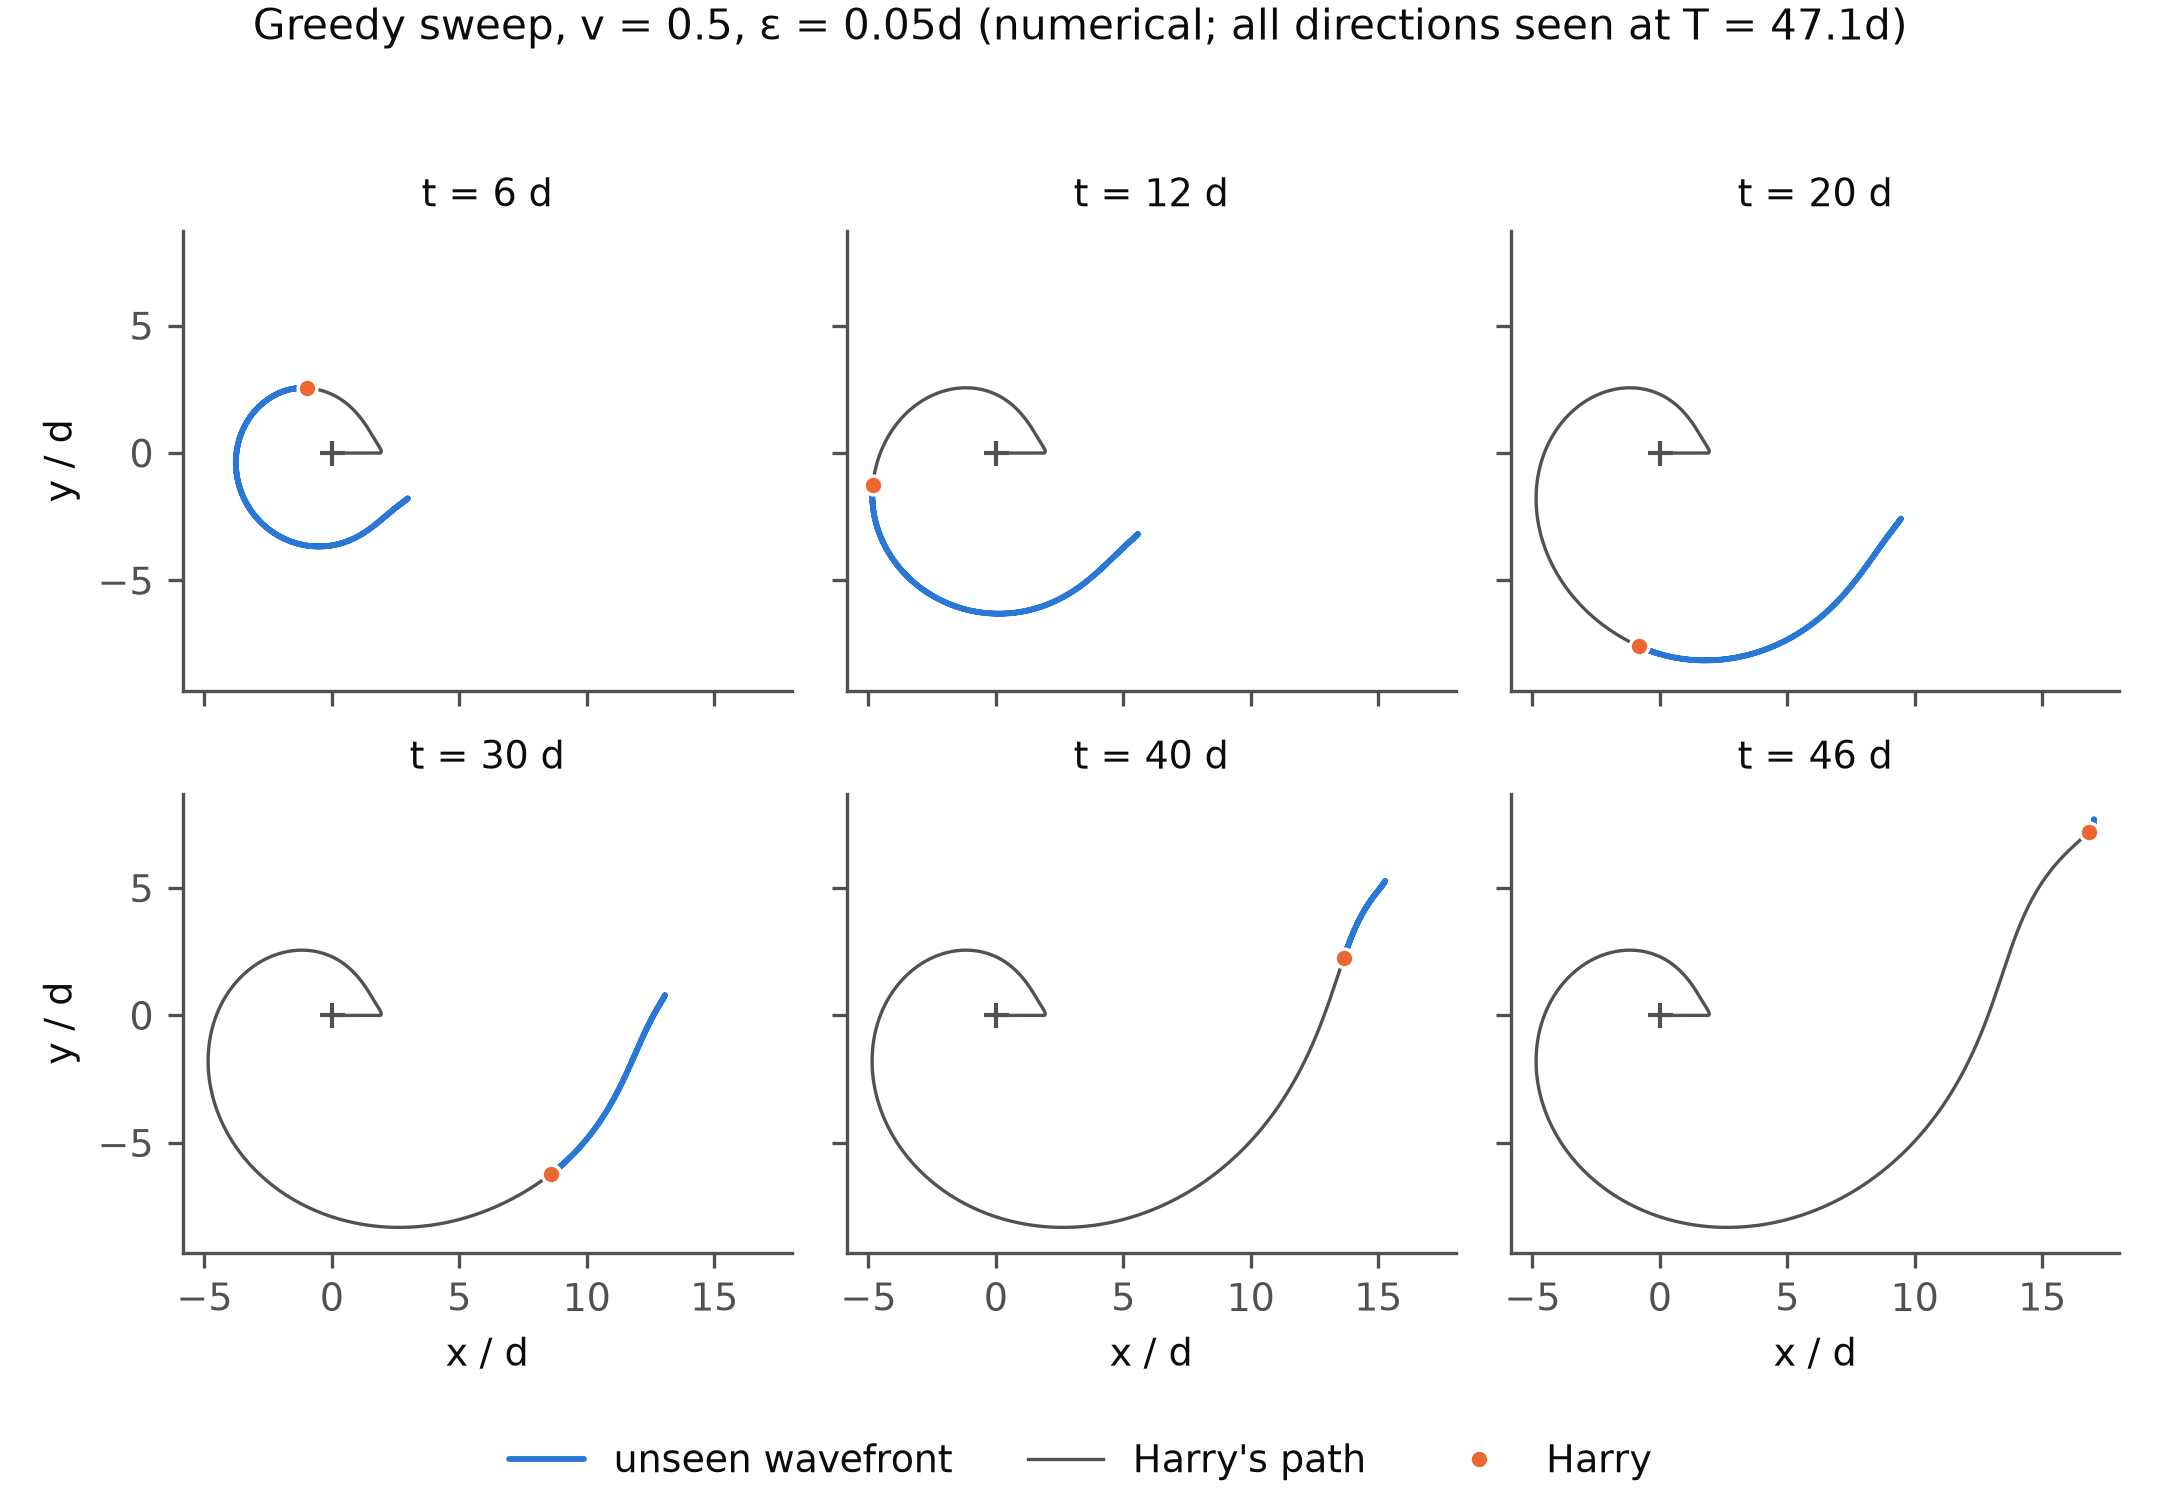
\includegraphics[width=\textwidth]{fig_paths.png}}{}
\caption{Greedy sweep at $v=0.5$, $\varepsilon=0.05d$ (numerical): the unseen part of the wavefront, Harry's path and Harry's position.}
\label{fig:paths}
\end{figure}
\begin{figure}[ht]\centering
\IfFileExists{fig_T.png}{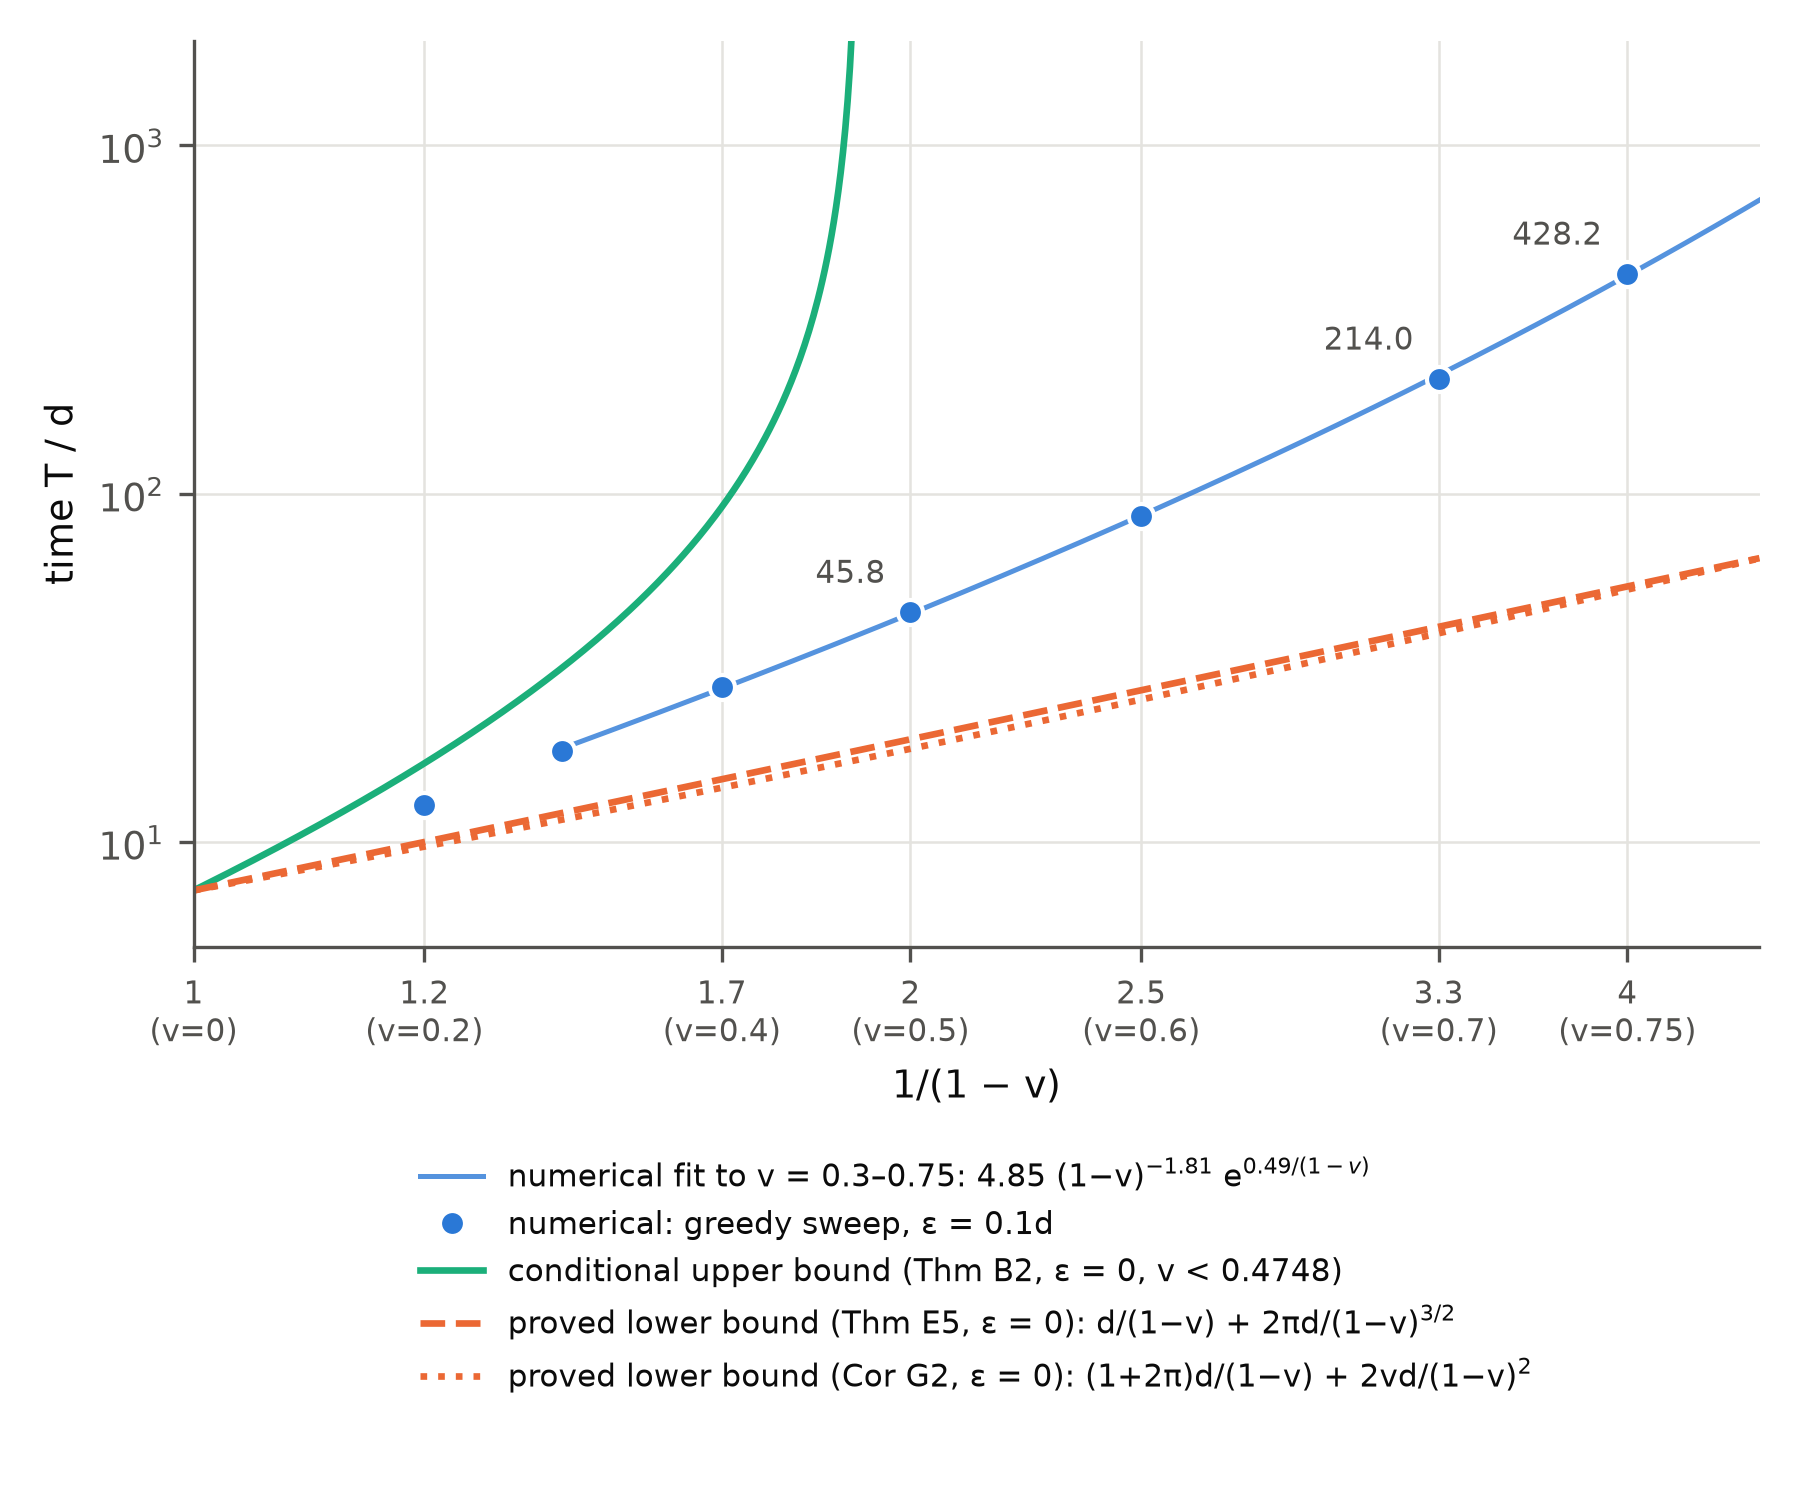
\includegraphics[width=0.8\textwidth]{fig_T.png}}{}
\caption{Sweep time against $1/(1-v)$: numerical greedy sweeps ($\varepsilon=0.1d$) and fit; the proved lower bounds of
Theorem~\ref{thm:E5} and Section~\ref{sec:G}; and the conditional upper bound of Theorem~\ref{thm:B2}. The bounds are for $\varepsilon=0$, so
the comparison is of orders of magnitude.}
\label{fig:T}
\end{figure}
\begin{figure}[ht]\centering
\IfFileExists{fig_v08.png}{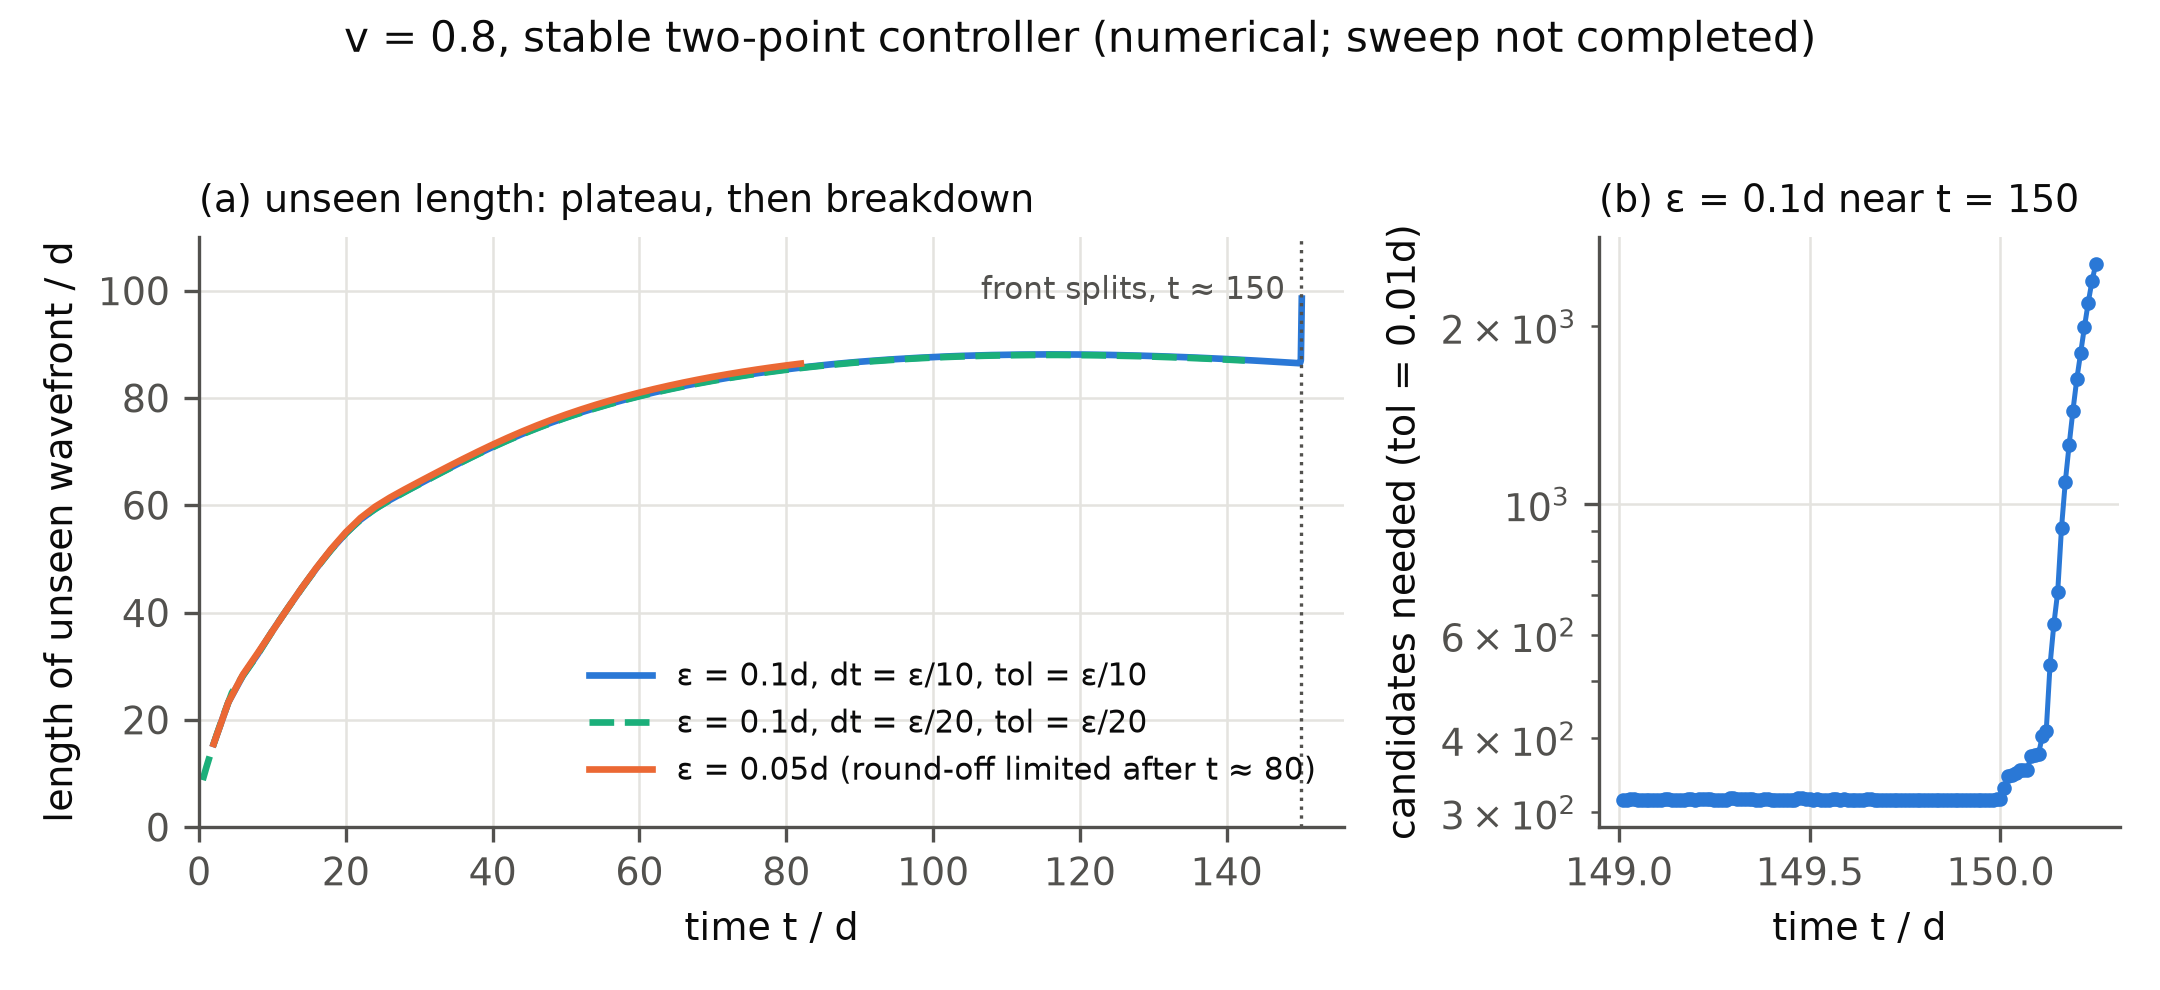
\includegraphics[width=\textwidth]{fig_v08.png}}{}
\caption{$v=0.8$ with a linearly stable two-point controller (numerical): unseen length against time, and the apparent breakdown at $t\approx150$, which extended-precision reruns show to be a double-precision artefact (report F2-1).}
\label{fig:v08}
\end{figure}
\end{document}
